\part{The /kə/ <\armenian{կը}> branch}
\begin{adjarianpage}\label{page:103}\end{adjarianpage}% should be 103

The /kə/ <\armenian{կը}> branch has 21 dialects:

\begin{enumerate}
	\item Dialect of Karin (\S\ref{chapter:Karin})
	\item Dialect of Mush (\S\ref{chapter:Mush})
	\item Dialect of Van (\S\ref{chapter:Van})
	\item Dialect of Tigranakert (\S\ref{chapter:Tigranakert})
	\item Dialect of Kharberd and Yerznka (\S\ref{chapter:Kharberd-Yerznka})
	\item Dialect of Şebinkarahisar (\S\ref{chapter:Şebinkarahisar})
	\item Dialect of Trabzon (\S\ref{chapter:Trabzon}) 
	\item Dialect of Hamshen (\S\ref{chapter:Hamshen})
	\item Dialect of Malatya (\S\ref{chapter:Malatya})
	\item Dialect of Cilicia (\S\ref{chapter:Cilicia})
	\item Dialect of Syria (\S\ref{chapter:Syria})
	\item Dialect of Arapgir (\S\ref{chapter:Arapgir})
	\item Dialect of Akn (\S\ref{chapter:Akn})
	\item Dialect of Sebastia (\S\ref{chapter:Sebastia})
	\item Dialect of Evdokia (\S\ref{chapter:Evdokia})
	\item Dialect of Smyrna (\S\ref{chapter:Smyrna})
	\item Dialect of Nicomedia (\S\ref{chapter:Nicomedia})
	\item Dialect of Istanbul (\S\ref{chapter:istanbul})
	\item Dialect of Rodosto (\S\ref{chapter:Rodosto})
	\item Dialect of Crimea (\S\ref{chapter:Crimea})
	\item Dialect of Austro-Hungary (\S\ref{chapter:Austro-Hungary})
	
	
\end{enumerate}

\chapter{Karin}\label{chapter:Karin}
\section{Background}
\begin{adjarianpage}\label{page:104}\end{adjarianpage}% should be 104


The center of this widely-spread dialect is Karin (Turkish: Erzurum). From the south, it spreads until near Hınıs, but without entering this small town (\armenian{աւան}). From the west, it reaches until Yerznka and Gümüşhane. During the last two Russo-Turkish wars, large migrant communities spread from the eastern and northern borders of this dialect to very far places, until Yerevan and Tbilisi. Four cities of the Caucasus (Kars, Alexandropol, Akhalkalak, and Akhaltskha) were filled with these same migrants, and now the entire Armenian population of those cities speaks the same dialect as the Armenians of Karin. 

\section{Phonology}

\subsection{Segment inventory}

\subsubsection{Vowels}
When we compare the phonetic system of this dialect against Old Armenian, we see that the vowels have been preserved almost unchanged. This dialect knows how to distinguish the sounds /i̯e/ <\armenian{ե}> vs. /e/ <\armenian{է}>, and /u̯o/ <\armenian{ո}> vs. /o/ <\armenian{օ}>. The vowel /æ/ <\armenian{ա̈} > is included. The vowels /œ, ʏ/ <\armenian{էօ, իւ}> are found in those words that are taken from Turkish; they do not exist at all in native Armenian words. Meanwhile in other dialects, such as Karabakh, Agulis, and even Istanbul, these vowels are found even in native words because of natural sound changes.

\paragraph{Vowel /æ/ <\armenian{ա̈} >}
The sound /æ/ <\armenian{ա̈} > in Karin is also foreign, and it is found primarily in loanwords from Turkish. But there are also some Armenian words where this sound has entered, whether because of Turkish influence or because of independent sound changes (Table \ref{tab:Karin:phono:segment:vowel:ae}).

\begin{table}[H]
	\centering
	\caption{Presence of the vowel /æ/ <\armenian{ա̈} > in the Karin dialect}
	\label{tab:Karin:phono:segment:vowel:ae}
	\resizebox{\textwidth}{!}{%
	\begin{tabular}{|l| ll|ll| ll|}
		\hline & \multicolumn{2}{l|}{Classical Armenian} &\multicolumn{2}{l|}{> Karin} & \multicolumn{2}{l|}{cf. SEA} \\ 
		`sugar' & ʃɑkʰɑɾ & \armenian{շաքար}& ʃækʰæɾ & \armenian{շա̈քա̈ր} & ʃɑkʰɑɾ & \armenian{շաքար} \\ 
		`beam' & mɑɾdɑk & \armenian{մարդակ}& mæɾtʰæk & \armenian{մա̈րթա̈կ} & mɑɾtʰɑkn & \armenian{մարդակ} \\ 
		`marble' & mɑɾmɑɾ & \armenian{մարմար}& mæɾmæɾ & \armenian{մա̈րմա̈ր} & mɑɾmɑɾ & \armenian{մարմար} \\ 
		`to bleat' & mɑjel & \armenian{մայել}& mæjel & \armenian{մա̈յէլ} & mɑjel & \armenian{մայել} \\ 
		`Sunday' & kiɾɑkē & \armenian{կիրակէ}& kiɾæki & \armenian{կիրա̈կի} & kiɾɑki & \armenian{կիրակի} \\ 
		\hline 
	\end{tabular}
}
\end{table}


The first three... 




\begin{adjarianpage}\label{page:105}\end{adjarianpage}% should be 105


... are also used in Turkish, and the influence of Turkish is probable. But the latter three words are native Armenian words.

\paragraph{Diphthongs /u̯o, i̯e/ <\armenian{ո, ե}>}

The sounds <\armenian{ո, ե}> have a diphthongal pronunciation /u̯o, i̯e/ <\armenian{ուօ, իէ}>, and they originate from the Classical Armenian mid vowels /o, e/ <\armenian{ո, ե}>; they are found only in the language of villagers. Urban speakers do not have these sounds. As for migrants of the Caucasus, those people who have a rural origin likewise pronounce the reflexes of Classical /o, ō/ <\armenian{ո, օ}> with a certain pronunciation; while those who are urban folk do not use these sounds. 

\subsubsection{Consonants}

\paragraph{Origin of the fricative /f/ <\armenian{ֆ}>}
For the consonants, let us first talk about the sound /f/ <\armenian{ֆ}>. 

The sound /f/ <\armenian{ֆ}> has two origins. First, it is found in foreign words that are borrowed from Turkish. Second, it developed in Armenian via natural sound changes. This latter origin also has two routes. 

\subparagraph{First route of origin for /f/}

Word-initially, the Classical sound /h/ <\armenian{հ}> becomes /f/ <\armenian{ֆ}> before Classical /o/ <\armenian{ո}> (\translatorHD{which became /uo̯/}) (Table \ref{tab:Karin:phono:segment:cons:f:1}).\footnote{\translatorHD{For the word `here', Adjarian provides an ancestor form <\armenian{հոս}>, but this form is not clearly attested in Classical Armenian. I treat it as a reconstruction. For `article', Adjarian provides an ancestor <\armenian{հոդ}>, but such a form does not exist but is instead <\armenian{յոդ}>. }}


\begin{table}[H]
	\centering
	\caption{Origin of /f/ <\armenian{ֆ}> from word-initial /h/ <\armenian{հ}> in the Karin dialect}
	\label{tab:Karin:phono:segment:cons:f:1}
	\begin{tabular}{|l| ll|ll| ll|}
		\hline & \multicolumn{2}{l|}{Classical Armenian} &\multicolumn{2}{l|}{> Karin} & \multicolumn{2}{l|}{cf. SEA} \\ 
		`earth' &hoɫ & \armenian{հող} & fu̯oʁ & \armenian{ֆող} & hoʁ & \armenian{հող} \\
		`smell' & hot & \armenian{հոտ} & fu̯ot & \armenian{ֆոտ} & hot & \armenian{հոտ} \\ 
		`hole (CA); pit (SEA)' &hoɾ & \armenian{հոր} & foɾ & \armenian{ֆոր} & hoɾ & \armenian{հոր} \\ 
		`here' &*hos & *\armenian{հոս} & fu̯os & \armenian{ֆոս} & hos & \armenian{հոս} \\
		`article' & jɑu̯d & \armenian{յաւդ} & fu̯od & \armenian{ֆոդ} & hod & \armenian{հոդ} \\ 
		`there' & hon & \armenian{հոն} & fu̯on & \armenian{ֆոն} & hon & \armenian{հոն} \\
		\hline 
	\end{tabular}
\end{table}

However, next to Classical /ɑu̯/ <\armenian{աւ}> (\translatorHD{which became /ō/ <\armenian{օ}>}), this change does not happen (Table \ref{tab:Karin:phono:segment:cons:f:1h}). 


\begin{table}[H]
	\centering
	\caption{Words with word-initial /h/ <\armenian{հ}> in the Karin dialect}
	\label{tab:Karin:phono:segment:cons:f:1h}
	\begin{tabular}{|l| ll|ll| ll|}
		\hline & \multicolumn{2}{l|}{Classical Armenian} &\multicolumn{2}{l|}{> Karin} & \multicolumn{2}{l|}{cf. SEA} \\ 
		`father.{\gen}' &hɑu̯ɾ & \armenian{հաւր} & hoɾ & \armenian{հօր} & hoɾ & \armenian{հոր} \\ \hline 
	\end{tabular}
\end{table}


It is notable that this sound change is specific to the rural language. The urban sound /h/ <\armenian{հ}> sound stays unchanged, and the reason for this is as follows. As can be seen above, the origin of the sound /f/ <\armenian{ֆ}> is the diphthongal pronunciation /u̯o/ <\armenian{ուօ}> of the reflex of Classical /o/ <\armenian{ո}>, because no such change occurs next to the reflex of Classical /ɑu̯/ <\armenian{աւ}> (\translatorHD{also written as /ō/ <\armenian{օ}>}). Now, because urban folk don't have the sound /u̯o/ <\armenian{ո}> and pronounce it as just /o/ <\armenian{օ}>, then naturally they do not have this type of /f/ <\armenian{ֆ}>.

\subparagraph{Second route of origin for /f/}

The second route for the origin of the sound /f/ <\armenian{ֆ}> is the sound /v/ <\armenian{վ}>, which gets devoiced to /f/ <\armenian{ֆ}> (Table \ref{tab:Karin:phono:segment:cons:f:2}).



\begin{table}[H]
	\centering
	\caption{Origin of /f/ <\armenian{ֆ}> from devoiced /v/ <\armenian{վ}> in the Karin dialect}
	\label{tab:Karin:phono:segment:cons:f:2}
	\resizebox{\textwidth}{!}{%
	\begin{tabular}{|l| ll|ll| ll|}
		\hline & \multicolumn{2}{l|}{Classical Armenian} &\multicolumn{2}{l|}{> Karin} & \multicolumn{2}{l|}{cf. SEA} \\ 
		`equal' &hɑ{wɑ}sɑɾ & \armenian{հաւասար} & hɑfsɑɾ & \armenian{հաֆսար} & hɑvɑsɑɾ & \armenian{հավասար} \\
		`to be gathered' & hɑ{wɑ}kʰil & \armenian{հաւաքիլ} & hɑfkʰil & \armenian{հաֆքիլ} & hɑvɑkʰvel & \armenian{հավաքվել} \\
		`to be able to (CA);  & bovel & \armenian{բովել} & bʰoɾfel & \armenian{բՙօրֆէլ} & bovel & \armenian{բովել} \\
  to roast (SEA)' & & & & & &  \\
		`south' & hɑɾɑu̯ & \armenian{հարաւ} & hɑɾɑf & \armenian{հարաֆ} & hɑɾɑv & \armenian{հարավ} \\
		`to mew' & nu̯ɑl & \armenian{նուալ} & nfɑl & \armenian{նֆալ} & nəvɑl & \armenian{նվալ} \\
		\hline 
	\end{tabular}
}
\end{table}

\paragraph{Consonant voicing}

In the consonant series, the Karin dialect has undergone a huge innovation, just as the Mush dialect has. 

We know that Old Armenian distinguished three groups of consonants. The Karin dialect has added a fourth series, entirely different from the others, which we called the voiced aspirates (Armenian: \textit{\armenian{թրթռուն շնշաւոր}}, French: \textit{sonore aspiree}). We represent them as /bʰ, ɡʰ, dʰ, d͡zʰ, d͡ʒʰ/ <\armenian{բՙ, գՙ, դՙ, ձՙ, ջՙ}>. Among the European phoneticians, Sievers was the first to notice the existence of voiced aspirates... 



\begin{adjarianpage}\label{page:106}\end{adjarianpage}% should be 106

... in the pronunciation of Ashtarak (a Yerevan dialect),\footnote{\translatorHD{The prose is unclear, but I suspect he means \citet{sievers-1901-grundzuge}[436, 442], based on a similar citation by \citet[438]{Schirru-2012-LaryngealFeatureArmenianDialect}. I couldn't verify this however. }} but no person focused in depth on these sounds. And the existence of four degrees of consonants in Armenia is a novelty. For the first time, I had the opportunity to use an experimental method to study these same sounds in Paris, using the phonetic machines (\armenian{ձայնագիտական մեքենաներ}) of Abbé Rousselot (Jean-Pierre Rousselot, Armenian: \armenian{Աբբա Ռուսլօ}), with young people from Mush, Sebastia, and others. The results of this study were published in a small work, where they present the four degrees of plosive letters in Armenian according to the pronunciation of six vernaculars (Istanbul, Aslanbeg, Nukha, Shushi, Sebastia, and Mush), summarized in four phototype images (\armenian{լուսատիպ պատկերներ}). See \citet{Adjarian-1899-ArmenianExplosives}. 

I ascertained the existence of four degrees of consonants a year later in my study of the Suceava dialect (see \citetitle{Bazmaveb}, 1899, page 219-220). Because we consider it excessive to further talk about this matter, we refer readers to the study. In passing, we only state that the pronunciation of the voiced aspirate consonants is close to the sounds /bh, ɡh, dh, d͡zh, d͡ʒh/ <\armenian{բհ, գհ, դհ, ձհ, ջհ}>, and these sounds are similar in manner to the Sanskrit consonants <bh, gh, dh, jh>. 

And thus we see a general picture of the plosive consonants of the Karin dialect (Table \ref{tab:Karin:phono:segment:cons:voice:voiceaspriate}).

\begin{table}[H]
	\caption{Voiced aspirates in the Karin dialect}\label{tab:Karin:phono:segment:cons:voice:voiceaspriate}\centering 
\resizebox{\textwidth}{!}{%
	\begin{tabular}{|l|ll|ll|ll|ll|}
		\hline & \multicolumn{2}{l|}{Voiced} & \multicolumn{2}{l|}{Voiced aspirate} & \multicolumn{2}{l|}{Voiceless} & \multicolumn{2}{l|}{Voiceless aspirate} \\
		Armenian name & \multicolumn{2}{l|}{\armenian{թրթռուն}} & \multicolumn{2}{l|}{\armenian{թրթռուն շնչաւոր}} & \multicolumn{2}{l|}{\armenian{խուլ}} & \multicolumn{2}{l|}{\armenian{խուլ շնչաւոր}} \\
		French name &\multicolumn{2}{l|}{sonore} & \multicolumn{2}{l|}{sonore asp.} & \multicolumn{2}{l|}{sourde} & \multicolumn{2}{l|}{sourde asp.} \\
		\hline & b &\armenian{բ} & bʰ& \armenian{բՙ} & p & \armenian{պ} & pʰ& \armenian{փ} \\
		& ɡ &\armenian{գ} & ɡʰ & \armenian{գՙ} & k & \armenian{կ} & kʰ & \armenian{ք} \\
		&d& \armenian{դ} & dʰ & \armenian{դՙ} & t & \armenian{տ} & tʰ & \armenian{թ} \\
		&d͡z& \armenian{ձ} & d͡zʰ& \armenian{ձՙ} & t͡s & \armenian{ծ} & t͡sʰ & \armenian{ց} \\
		& d͡ʒ &\armenian{ջ} & d͡ʒʰ & \armenian{ջՙ} & t͡ʃ & \armenian{ճ} & t͡ʃʰ & \armenian{չ} 
		\\ \hline 
	\end{tabular}
}
\end{table}

\paragraph{Voiced glottal fricative /ɦ/ <\armenian{յ̵}> }

In the Karin dialect, the reflex of the Classical sound /j/ <\armenian{յ}> has a pronunciation similar to the voiced aspirates; this sound is also found in the Mush dialect, and we represent it as /ɦ/ <\armenian{յ̵}>. This sound is found against the Old Armenian sound /j/ <\armenian{յ}> (Table \ref{tab:Karin:phono:segment:cons:hh}).




\begin{table}[H]
	\centering
	\caption{Voiced glottal fricative /ɦ/ <\armenian{յ̵}> in the Karin dialect}
	\label{tab:Karin:phono:segment:cons:hh}
\resizebox{\textwidth}{!}{%
	\begin{tabular}{|l| ll|ll| ll|}
		\hline & \multicolumn{2}{l|}{Classical Armenian} &\multicolumn{2}{l|}{> Karin} & \multicolumn{2}{l|}{cf. SEA} \\ 
		given name &jɑɾutʰiu̯n & \armenian{Յարութիւն} & ɦɑɾutʰ & \armenian{յ̵արութ} & hɑɾutʰjun & \armenian{Հարություն} \\
		given name &jɑkob & \armenian{Յակոբ} & ɦɑko & \armenian{յ̵ակօ} & hɑkopʰ & \armenian{Հակոբ} \\
		\hline 
	\end{tabular}
}
\end{table}


With this, the dialect has two types of glottal (\armenian{հագագային}) sounds: /ɦ, h/ <\armenian{յ̵}, \armenian{հ}>. 


\begin{adjarianpage}\label{page:107}\end{adjarianpage}% should be 107

\subsection{Sound changes}

The Karin dialect is not very rich in sound changes; and after indicating the above cases, few things remain. 

\subsubsection{Monophthongal vowel changes}
\paragraph{Vowel syncope of Classical Armenian /ɑ/ <\armenian{ա}>}
As general rule for all dialects in the /kə/ <\armenian{կը}> branch, in polysyllabic words, the reflex of the Classical vowel /ɑ/ <\armenian{ա}> of a word-medial syllable is deleted or changes to /ə/ <\armenian{ը}> (Table \ref{tab:Karin:phono:segment:cons:f:2}). We don't return to this general rule elsewhere. 



\begin{table}[H]
	\centering
	\caption{Medial vowel syncope in various Western dialects (Karin, Istanbul)}
	\label{tab:Karin:phono:change:vowel:syncope}
\resizebox{\textwidth}{!}{%
	\begin{tabular}{|l|ll ll ll|}
	\hline	&\multicolumn{2}{l}{`to recognize' }&\multicolumn{2}{l}{`sickly'} &\multicolumn{2}{l|}{`mouth-{\gen} } \\	\hline
		Classical Armenian & t͡ʃɑnɑt͡ʃʰel & \armenian{ճանաչել}
		& hi{wɑ}ndot & \armenian{հիւանդոտ} & beɾɑn-i & \armenian{բերանի}
		\\
		> Karin& t͡ʃɑnt͡ʃʰel & \armenian{ճանչել}
		& hivəndu̯ot& \armenian{հիվընդոտ} 
		& bʰeɾn-i &\armenian{բՙէրնի} 
		\\
		cf. Istanbul &t͡ʃɑʃnɑl & \armenian{ճաշնալ}
		& hivɑndod, & \armenian{հիվանդօդ},
		& beɾn-i& \armenian{բէրնի} 
		\\
		& & & hivəndod & \armenian{հիվընդօդ} & & 
		\\
		cf. SWA & d͡ʒɑnt͡ʃʰnɑl & \armenian{ճանչնալ} 
		& hivɑntʰod & \armenian{հիւանդոտ}
		&pʰeɾn-i & \armenian{բերնի}
		\\
		cf. SEA & t͡ʃɑnɑt͡ʃʰel & \armenian{ճանաչել}
		& hivɑndot & \armenian{հիվանդոտ} 
		&beɾɑn-i & \armenian{բերանի}
		\\	\hline
 	\end{tabular}
}
\end{table}


\paragraph{Classical Armenian /e/ <\armenian{ե}>}


At the beginning of monosyllabic words (Table \ref{tab:Karin:phono:change:vowel:e}a), the Classical sound /e/ <\armenian{ե}> has turned to /je/ <\armenian{յէ}> or /ji̯e/ <\armenian{յե}> (the latter for villagers). At the beginning of polysyllabic words, the sound is /e/ <\armenian{է}> (Table \ref{tab:Karin:phono:change:vowel:e}b). And word-medially, it is /e/ <\armenian{է}> or /i̯e/ <\armenian{ե}> (Table \ref{tab:Karin:phono:change:vowel:e}c). 




\begin{table}[H]
	\centering
	\caption{Change from Classical Armenian /e/ <\armenian{ե}> to /je, ji̯e, e, i̯e/ <\armenian{յէ, յե, է, ե}> in the Karin dialect}
	\label{tab:Karin:phono:change:vowel:e}
	\resizebox{\textwidth}{!}{%
		\begin{tabular}{|ll| ll|ll| ll|}
		\hline & & \multicolumn{2}{l|}{Classical Armenian} &\multicolumn{2}{l|}{> Karin} & \multicolumn{2}{l|}{cf. SEA} \\ 
		a. & `ox' & ezən & \armenian{եզն} & jez & \armenian{յէզ} & jez & \armenian{եզ} \\
		& `boiling (CA);  & er-kʰ (-{\pl}) & \armenian{եռք} & jerkʰ & \armenian{յէռք} & jer-kʰ & \armenian{եռք} \\
		&  tingling (SEA)' && & & & & \\
		&`I' & es & \armenian{ես} & jes & \armenian{յէս} &jes & \armenian{ես} \\
		& `when' & eɾb & \armenian{երբ} & jepʰ & \armenian{յէփ} & jeɾpʰ & \armenian{երբ} \\
		& `cooking' & epʰ & \armenian{եփ} & jepʰ & \armenian{յէփ} & jepʰ & \armenian{եփ} \\
				b. & `to cook' & epʰel & \armenian{եփել} & epʰel & \armenian{էփէլ} & jepʰel & \armenian{եփել} \\
		& `dream' & eɾɑz & \armenian{երազ} & eɾɑz & \armenian{էրազ} & jeɾɑz & \armenian{երազ} \\
		c. & `to bring' & beɾel & \armenian{բերել} & bʰeɾel & \armenian{բՙէրէլ} & beɾel & \armenian{բերել} \\
		& `big' &met͡s & \armenian{մեծ} & met͡s (urban) & \armenian{մէծ} &met͡s & \armenian{մեծ} \\
		& & & & mi̯et͡s (villager) & \armenian{մեծ} & & \\
		\hline 
	\end{tabular}
}
\end{table}


\paragraph{Classical Armenian /o/ <\armenian{ո}>}


At the beginning of monosyllabic words, the Classical sound /o/ <\armenian{ո}> (Table \ref{tab:Karin:phono:change:vowel:o}) has changed to /vo/ <\armenian{վօ}>, /o/ <\armenian{օ}>, or /vu̯o/ <\armenian{վո}>; at the beginning of polysyllabic words to /o/ <\armenian{օ}>; and word-medially to /o/ <\armenian{օ}> or /u̯o/ <\armenian{ո}> (the forms /vu̯o, u̯o/ <\armenian{վո, ո}> are rural). The word for `who' has a typical form /vev/ <\armenian{վէվ}>. 




\begin{table}[H]
	\centering
	\caption{Change from Classical Armenian /o/ <\armenian{ո}> to /vo, o, vu̯o, u̯o, ve/ <\armenian{վօ, օ, վո, ո, վէ}> in the Karin dialect}
	\label{tab:Karin:phono:change:vowel:o}
	\resizebox{\textwidth}{!}{%
	\begin{tabular}{| l| ll|ll| ll|}
		\hline & \multicolumn{2}{l|}{Classical Armenian} &\multicolumn{2}{l|}{> Karin} & \multicolumn{2}{l|}{cf. SEA} \\ 
		`that' & oɾ & \armenian{որ} & voɾ & \armenian{վօր} & voɾtʰi & \armenian{որ} \\
		`to take pity on' & oɫoɾmil & \armenian{ողորմիլ} & oʁoɾmil & \armenian{օղօրմիլ} & voʁoɾmel & \armenian{ողորմել} \\
		`to ruminate' & oɾot͡ʃɑl & \armenian{որոճալ} & oɾot͡ʃɑl & \armenian{օրօճալ} & voɾot͡ʃɑl & \armenian{որոճալ} \\
		`who' & ov & \armenian{ով} & vev & \armenian{վէվ} & ov & \armenian{ով} \\ 
		\hline 
	\end{tabular}
}
\end{table}

\subsubsection{Diphthong changes}

\paragraph{Classical Armenian /ɑi̯/ <\armenian{այ}>}



The Classical Armenian diphthong /ɑi̯/ <\armenian{այ}> has changed to /ɑ/ <\armenian{ա}> for city people, and /e/ <\armenian{է}> for villagers. For settlements in the Caucasus, Akhaltskha has the form /ɑ/ <\armenian{ա}>, while Alexandropol has the form /e/ <\armenian{է}> (Table \ref{tab:Karin:phono:change:diphth:aj}). 



\begin{table}[H]
	\centering
	\caption{Change from Classical Armenian /ɑi̯/ <\armenian{այ}> to /ɑ, e/ <\armenian{ա, է}> in the Karin dialect}
	\label{tab:Karin:phono:change:diphth:aj}
	\begin{tabular}{| l| ll|ll| ll|}
		\hline & \multicolumn{2}{l|}{Classical Armenian} &\multicolumn{2}{l|}{> Karin} & \multicolumn{2}{l|}{cf. SEA} \\ 
		`father' & hɑi̯ɾ & \armenian{հայր} & hɑɾ, heɾ & \armenian{հար, հէր} & hɑjɾ & \armenian{հայր} \\ 
		`wood' & pʰɑi̯t & \armenian{փայտ} & pʰɑt, pʰet & \armenian{փատ, փէտ} &pʰɑjt & \armenian{փայտ} \\
		`mother' & mɑi̯ɾ & \armenian{մայր} & mɑɾ, meɾ & \armenian{մար, մէր} & mɑjɾ & \armenian{մայր} \\
		`goat' & ɑi̯t͡s & \armenian{այծ} & ɑt͡s, et͡s & \armenian{ած, էծ} & ɑjt͡s & \armenian{այծ} \\ 
		\hline 
	\end{tabular}
\end{table}


\paragraph{Classical Armenian /oi̯/ <\armenian{ոյ}>}


The Classical Armenian diphthong /oi̯/ <\armenian{ոյ}> changed to /u/ <\armenian{ու}> (Table \ref{tab:Karin:phono:change:diphth:oj}). 




\begin{table}[H]
	\centering
	\caption{Change from Classical Armenian /oi̯/ <\armenian{ոյ}> to /u/ <\armenian{ու}> in the Karin dialect}
	\label{tab:Karin:phono:change:diphth:oj}
	\begin{tabular}{| l| ll|ll| ll|}
		\hline & \multicolumn{2}{l|}{Classical Armenian} &\multicolumn{2}{l|}{> Karin} & \multicolumn{2}{l|}{cf. SEA} \\ 
		`weak' & tʰoi̯l & \armenian{թոյլ} & tʰul & \armenian{թուլ} & tʰujl & \armenian{թույլ} \\ 
		`blue' & kɑpoi̯t & \armenian{կապոյտ} & kɑput & \armenian{կապուտ} & kɑpujt & \armenian{կապույտ} \\ 
		`light' & loi̯s & \armenian{լոյս}& lus & \armenian{լուս} & lujs & \armenian{լույս} \\
		\hline 
	\end{tabular}
\end{table}


\paragraph{Classical Armenian /iu̯/ <\armenian{իւ}>}


The Classical Armenian diphthong /iu̯/ <\armenian{իւ}> changed to /u/ <\armenian{ու}> (Table \ref{tab:Karin:phono:change:diphth:iu̯}). 




\begin{table}[H]
	\centering
	\caption{Change from Classical Armenian /iu̯/ <\armenian{իւ}> to /u/ <\armenian{ու}> in the Karin dialect}
	\label{tab:Karin:phono:change:diphth:iu̯}
	\begin{tabular}{| l| ll|ll| ll|}
		\hline & \multicolumn{2}{l|}{Classical Armenian} &\multicolumn{2}{l|}{> Karin} & \multicolumn{2}{l|}{cf. SEA} \\ 
 
		`flour' & ɑliu̯ɾ & \armenian{ալիւր} & ɑluɾ & \armenian{ալուր} & ɑljuɾ & \armenian{ալյուր} \\ 
		`fountain' & ɑɫbiu̯ɾ & \armenian{աղբիւր} & ɑχbʰuɾ & \armenian{ախբՙուր} & ɑχpjuɾ & \armenian{աղբյուր} \\ 
		`snow' & d͡ziu̯n & \armenian{ձիւն}& d͡zʰun & \armenian{ձՙուն} & d͡zjun & \armenian{ձյուն} \\
		\hline 
	\end{tabular}
\end{table}

\subsubsection{Consonant changes}

\paragraph{Voicing changes}
For the consonants, the Old Armenian voiceless unaspirates and voiceless aspirates remain unchanged. The voiced sound have become voiced aspirates in general; but after nasals, they remain voiced unaspirated (Table \ref{tab:Karin:phono:change:cons:voice}). 




\begin{table}[H]
	\centering
	\caption{Voicing changes for stops and affricates in the Karin dialect}
	\label{tab:Karin:phono:change:cons:voice}
	\resizebox{\textwidth}{!}{%
	\begin{tabular}{| l| ll|ll| ll|}
		\hline & \multicolumn{2}{l|}{Classical Armenian} &\multicolumn{2}{l|}{> Karin} & \multicolumn{2}{l|}{cf. SEA} \\ 
		`thing' &bɑn & \armenian{բան} & bʰɑn & \armenian{բՙան} & bɑn & \armenian{բան} \\
		`mouth' & beɾɑn & \armenian{բերան} & bʰeɾɑn &\armenian{բՙէրան} & beɾɑn & \armenian{բերան} \\
		`hand' &d͡zer-kʰ (plural) & \armenian{ձեռք} & d͡zʰerkʰ & \armenian{ձՙէռք} &d͡zerkʰ & \armenian{ձեռք} \\
		`I.{\dat}' &ind͡z& \armenian{ինձ} & ind͡zi & \armenian{ինձի} &ind͡z & \armenian{ինձ} \\
		`apple' & χənd͡zoɾ & \armenian{խնձոր} & χənd͡zoɾ & \armenian{խընձօր} & χənd͡zoɾ & \armenian{խնձոր} \\ 
		`cat' &kɑtu & \armenian{կատու} & kɑtu & \armenian{կատու} & kɑtu & \armenian{կատու} \\ 
		`wool' & buɾd & \armenian{բուրդ} & bʰuɾdʰ & \armenian{բՙուրդՙ} & buɾtʰ & \armenian{բուրդ} \\ 
		`sour' &tʰətʰu & \armenian{թթու} & tʰətʰu & \armenian{թըթու} & tʰətʰu & \armenian{թթու} \\ 
		\hline 
	\end{tabular}
}
\end{table}

\paragraph{Assimilation of /t/ <\armenian{տ}> to a /r, t͡ʃ/ <\armenian{ր, ճ}>}

When the Classical sound /t/ <\armenian{տ}> is before the sounds /ɾ, r, t͡ʃ, ʒ/ <\armenian{ր, ռ, ճ, ժ}>, it assimilates to those sounds. Only in this situation does the Classical sound /ɾ/ <\armenian{ր}> become /r/ <\armenian{ռ}>, and the sound /ʒ/ <\armenian{ժ}> becomes /t͡ʃ/ <\armenian{ճ}> (Table \ref{tab:Karin:phono:change:cons:d}). 




\begin{table}[H]
	\centering
	\caption{Change from Classical Armenian /t/ <\armenian{տ}> to a /r, t͡ʃ/ <\armenian{ր, ճ}> in the Karin dialect}
	\label{tab:Karin:phono:change:cons:d}
	\resizebox{\textwidth}{!}{%
	\begin{tabular}{| l| ll|ll| ll|}
		\hline & \multicolumn{2}{l|}{Classical Armenian} &\multicolumn{2}{l|}{> Karin} & \multicolumn{2}{l|}{cf. SEA} \\ 
		`to tear' &pɑtɑrel & \armenian{պատառել} & pɑrrel & \armenian{պառռէլ} & pɑtɑrel, pɑtrel & \armenian{պատառել, պատռել} \\
		`to divide' &kətɾel & \armenian{կտրել} & krrel & \armenian{կռռէլ} & kətɾel & \armenian{կտրել} \\
		`to break' &kotoɾel & \armenian{կոտորել} & korrel & \armenian{կօռռէլ} & kotoɾel, kotɾel & \armenian{կոտորել, կոտրել} \\
		`ready' &pɑtɾɑst & \armenian{պատրաստ} & pɑrrɑst & \armenian{պառռաստ} & pɑtɾɑst & \armenian{պատրաստ} \\
		name `Peter' &petɾos & \armenian{Պետրոս} & perros & \armenian{Պէռռօս} & petɾos & \armenian{Պետրոս} \\
		`to punish' &pɑtʒel & \armenian{պատժել} & pɑt͡ʃt͡ʃel & \armenian{պաճճէլ} & pɑtʒel & \armenian{պատժել} \\
		`reason' &pɑtʒɑr & \armenian{պատճառ} & pɑt͡ʃt͡ʃɑr & \armenian{պաճճառ} & pɑtʒɑr & \armenian{պատճառ} \\
		\hline 
	\end{tabular}
}
\end{table}

\begin{adjarianpage}\label{page:108}\end{adjarianpage}% should be 108

\subsection{Lexical change}

The Classical verb /ɑrnel/ <\armenian{առնել}> `to do' becomes /enel/ <\armenian{էնէլ}>, whereas that word is /ɑnel/ <\armenian{անել}> or /ənel/ <\armenian{ընել}> in other places. \translatorHD{To clarify, the reflex of this verb is /ɑnel/ in SEA, and /ənel/ in SWA. }

\subsection{Stress}

In the Karin dialect, as in all the other dialects of the /kə/ <\armenian{կը}> branch, stress is on the last syllable. However, stress in Karin is an especially peculiar accent (\armenian{առագոնութիւն}) that it leaves a very pleasant impression. It is difficult for me to give a scientific explanation for this, but the following things are apparent. Stress in Karin is higher than the stress in other dialects; thus the difference in degree between unstressed and stressed syllables is very big. At the same time, because the pronunciation is more relaxed and elongated, during the descent, the sound goes through many musical notes, and it almost forms a song. 

\section{Morphology}
\subsection{Noun inflection or declension}

\subsubsection{Inflection for singular nouns}

Like all the dialects of the /kə/ <\armenian{կը}> branch, the Karin dialect has 6 cases, which are normative, genitive-dative, accusative, ablative, and instrumental. The locative is missing. 

However, the Karin dialect differ from the other dialects of the /kə/ <\armenian{կը}> branch; in the accusative, it distinguishes between animate and inanimate objects, similar to the /um/ <\armenian{ում}> branch. The accusative of inanimates is the same as the nominative, while the animates use the dative (\ref{sent:Karin:morpho:noun:DOM}). 


\begin{exe}
	\ex Karin \label{sent:Karin:morpho:noun:DOM}
	\begin{xlist}
		\ex \gll kɑtu-i-n səpɑn-e-t͡sʰ-i-$\emptyset$ \\ 
		cat-{\dat}-{\defgloss} kill-{\thgloss}-{\aor}-{\pst}-1{\sg} \\
		\trans `I killed the cat.'\\
		\armenian{կատուին սըպանէցի}
		\ex \gll kov-i-n moɾtʰ-e-t͡sʰ-i-$\emptyset$ \\ 
		cow-{\dat}-{\defgloss} slaughter-{\thgloss}-{\aor}-{\pst}-1{\sg} \\
		\trans `I slaughtered the cow.'\\
		\armenian{կօվին մօրթէցի}. 
	\end{xlist}
\end{exe}

As is the norm, the ablative uses the formative /-en/ <\armenian{էն}>, while the instrumental uses the formative /ov/ <\armenian{օվ}>. 

\subsubsection{Inflection for plural nouns}

In accordance with the general rule, the plural is formed with the formatives /-eɾ/ <\armenian{էր}> or /-neɾ/ <\armenian{նէր}>. But in this dialect, we also find the formative /estɑn/ <\armenian{Էստան}>. This formative is a reflex of the Old Armenian formative /-stɑn/ <\armenian{ստան}>, which is a location formative; the formative forms collective nouns and it can also receive the formative /neɾ/ <\armenian{նէր}> (Table \ref{tab:Karin:morpho:noun:pl}). 




\begin{table}[H]
	\centering
	\caption{Plural suffixes in the Karin dialect}
	\label{tab:Karin:morpho:noun:pl}
	\resizebox{\textwidth}{!}{%
	\begin{tabular}{| l|ll| ll|}
		\hline & \multicolumn{2}{l|}{Karin} & \multicolumn{2}{l|}{cf. SEA} \\ 
		`key-{\pl}' &bʰɑnl-estɑn & \armenian{բՙանլէստան} & bɑnɑli-neɾ & \armenian{բանալիներ} \\
		~ ~ \textit{or} &bʰɑnl-estən-neɾ & \armenian{բՙանլէստըննէր} & & \\
		`bathroom-{\pl}' &bʰɑʁn-estɑn & \armenian{բՙաղնէստան} & bɑʁnikʰ-neɾ & \armenian{բաղնիքներ} \\
		~ ~ \textit{or} &bʰɑʁn-estən-neɾ & \armenian{բՙաղնէստըննէր} & & \\
		`ring-{\pl}' &mɑtn-estɑn & \armenian{մատնէստան} & mɑtɑni-neɾ & \armenian{մատանիներ} \\
		`dormer.window-{\pl}' &eɾdʰ-estɑn & \armenian{էրդՙէստան} & jeɾtikʰ-neɾ & \armenian{երդիքներ} \\
		`intestine-{\pl}' &ɑʁ-estɑn & \armenian{աղէստան} & ɑʁikʰ-neɾ & \armenian{աղիքներ} \\
		`bride-{\pl}' &hɑɾsn-estɑn & \armenian{հարսնէստան} & hɑɾs-neɾ & \armenian{հարներ} \\
		`underpants-{\pl}' &vɑɾt-estɑn & \armenian{վարտէստան} & vɑɾtikʰ-neɾ & \armenian{վարտիքներ} \\
		`year-{\pl}' &tɑɾ-estɑn & \armenian{տարէստան} & tɑɾi-neɾ & \armenian{տարիներ} \\
		\hline 
	\end{tabular}
}
\end{table}



As we can see from the examples, this formative is placed only after words that end in /-ikʰ/ <\armenian{իք}>. \translatorHD{I don't understand this generalization because it seems falsified by Adjarian's data. }

The other case markers of the plural are like the those of the singular, except for the genitive-dative which, in all the /kə/ <\armenian{կը}> branch dialects, uses the form /-u/ <\armenian{ու}> (Table \ref{tab:Karin:morpho:noun:plGen}). 


\begin{table}[H]
	\centering
	\caption{Genitive-dative of the plural in the Karin dialect}
	\label{tab:Karin:morpho:noun:plGen}
	\resizebox{\textwidth}{!}{%
	\begin{tabular}{| l|ll| ll|}
		\hline & \multicolumn{2}{l|}{Karin} & \multicolumn{2}{l|}{cf. SEA} \\ 
		`city-{\pl}-{\gen}/{\dat}' &kʰɑʁɑkʰ-neɾ-u & \armenian{քաղաքներու} & kʰɑʁɑkʰ-neɾ-i & \armenian{քաղաքների} \\
		\hline 
	\end{tabular}
}
\end{table}



\begin{adjarianpage}\label{page:109}\end{adjarianpage}% should be 109

\subsection{Pronoun inflection or declension}

For pronouns, we note the following (Table \ref{tab:Karin:morphology:pronoun:sample}). 

\begin{table}[H]
	\centering
	\caption{Sample of pronouns in the Karin dialect}
	\label{tab:Karin:morphology:pronoun:sample}
	\begin{tabular}{|l ll| }
		\hline 
		personal 1SG {\nom} `I' &jes & \armenian{յէս} \\
		personal 2SG {\nom} `you' &dʰu & \armenian{դՙու} \\
		personal 1PL {\nom} `we' &menkʰ & \armenian{մէնք} \\
		personal 2PL {\nom} `you' &dʰukʰ & \armenian{դՙուք} \\
		demonstrative proximal {\sg} `this' & ɑs & \armenian{աս} \\
		demonstrative medial {\sg} `that' & ɑdʰ & \armenian{ադՙ} \\
		demonstrative distal {\sg} `that yonder' & ɑn & \armenian{ան} \\
		demonstrative proximal {\pl} `these' & ɑsonkʰ & \armenian{ասօնք} \\
		demonstrative medial {\pl} `those' & ɑtonkʰ & \armenian{ատօնք} \\
		demonstrative distal {\pl} `those yonder' & ɑnonkʰ & \armenian{անօնք} \\
		demonstrative proximal {\sg} `that' & isi & \armenian{իսի} \\
		demonstrative medial {\sg} `that' & iti & \armenian{իտի} \\
		demonstrative distal {\sg} `that yonder' & ini & \armenian{ինի} \\
		demonstrative proximal {\sg} `that' & isik & \armenian{իսիկ} \\
		demonstrative medial {\sg} `that' & itik & \armenian{իտիկ} \\
		demonstrative distal {\sg} `that yonder' & inik & \armenian{ինիկ} \\
		demonstrative proximal {\pl} `these' & isonkʰ & \armenian{իսօնք} \\
		demonstrative medial {\pl} `those' & itonkʰ & \armenian{իտօնք} \\
		demonstrative distal {\pl} `those yonder' & inonkʰ & \armenian{ինօնք} \\
		
		\hline 
	\end{tabular}
\end{table}

In accordance with the norm, the first ones are not a unique innovation. The latter words /isik, inik, inin/ <\armenian{իսիկ, իտիկ, ինիկ}> are un-declinable; the others are declined in the following way (Table \ref{tab:Karin:morpho:pronoun}). 


\begin{table}[H]
	\centering
	\caption{Demonstrative pronouns in the Karin dialect} \label{tab:Karin:morpho:pronoun}
	
		\resizebox{\textwidth}{!}{%
		\begin{tabular}{|l|lll|lll|}
		\hline & \multicolumn{3}{c|}{Singular} & \multicolumn{3}{c|}{Plural} \\
		& proximal & medial & distal & proximal & medial & distal \\
		& `this' & `that' & `yonder' & `these' & `those' & `those yonder' \\
		\hline {\nom} & isi & iti & ini & isonkʰ & itonkʰ & inonkʰ \\
		& \armenian{իսի} & \armenian{իտի} & \armenian{ինի} & \armenian{իսօնք} & \armenian{իտօնք} & \armenian{ինօնք} \\
	\hline	{\gen},{\dat} & isoɾ & itoɾ & inoɾ & isont͡sʰ & itont͡sʰ & inont͡sʰ \\
		& \armenian{իսօր} & \armenian{իտօր} & \armenian{ինօր} & \armenian{իսօնց} & \armenian{իտօնց} & \armenian{ինօնց} \\
		\hline {\abl} & isoɾ-en & itoɾ-en & inoɾ-en & isont͡sʰ-en & itont͡sʰ-en & inont͡sʰ-en \\
		& isoɾ-m-en & itoɾ-m-en & inoɾ-m-en & isont͡sʰ-m-en & itont͡sʰ-m-en & inont͡sʰ-m-en \\
		& \armenian{իսօրէն} & \armenian{իտօրէն} & \armenian{ինօրէն} & \armenian{իսօնցէն} & \armenian{իտօնցէն} & \armenian{ինօնցէն} \\
		& \armenian{իսօրմէն} & \armenian{իտօրմէն} & \armenian{ինօրմէն} & \armenian{իսօնցմէն} & \armenian{իտօնցմէն} & \armenian{ինօնցմէն} \\
		\hline {\ins} & isoɾ-ov & itoɾ-ov & inoɾ-ov & isont͡sʰ-ov & itont͡sʰ-ov & inont͡sʰ-ov \\
		& isoɾ-m-ov & itoɾ-m-ov & inoɾ-m-ov & isont͡sʰ-m-ov & itont͡sʰ-m-ov & inont͡sʰ-m-ov \\
		& \armenian{իսօրօվ} & \armenian{իտօրօվ} & \armenian{ինօրօվ} & \armenian{իսօնցօվ} & \armenian{իտօնցօվ} & \armenian{ինօնցօվ} \\
		& \armenian{իսօրմօվ} & \armenian{իտօրմօվ} & \armenian{ինօրմօվ} & \armenian{իսօնցմօվ} & \armenian{իտօնցմօվ} & \armenian{ինօնցմօվ} 
		\\ \hline
	\end{tabular}
}
\end{table}

\subsection{Verb inflection or conjugation}

\subsubsection{Indicative present and past imperfective: allomorphy of the indicative morpheme}

The formation of verbs is very similar. There are no tenses that are constructed with /-um/ <\armenian{ում}>, as in all the /kə/ <\armenian{կը}> dialects. The indicative present and imperfective are formed similar to Old Armenian, but here we add the formative /kə/ <\armenian{կը}>, which is placed at the end of the verb in the Karin dialect. 

Verbs that start with a vowel also receive the formative /k-/ <\armenian{կ}> at the beginning; the verbs /əllil/ <\armenian{ըլլիլ}> `to be', /əjnil/ <\armenian{ըյնիլ}> `to fall', /uzel/ <\armenian{ուզէլ}> `to want', etc. take the form /ɡʰ-/ <\armenian{գՙ}>. Monosyllabic verbs take /ku-/ <\armenian{կու}>; only the verb /ɡʰɑm/ <\armenian{գՙամ}> `I come' takes /ɡʰu/ <\armenian{գՙու}> (in assimilation with the verb's initial sound /ɡʰ/ <\armenian{գՙ}>). Thus are all the forms of these verbs:

\paragraph{Suffix or enclitic /kə/ for consonant-initial verbs}

\translatorHD{I clarify what he means. In Eastern dialects like SEA, the indicative present and past imperfective are formed periphrastically with a non-finite converb plus a finite auxiliary. But in Western dialects like SWA and Karin, these forms are created synthetically. Tense and inflection is on the finite verb, while the indicative mood is marked by adding a morpheme that looks like /kə/. In SWA, this morpheme is /ɡu-/ before monosyllabic roots, /ɡ-/ before vowels, and /ɡə-/ elsewhere before consonants. Karin uses cognates of these affix shapes with essentially the same distribution.}

\translatorHD{First consider a typical consonant-initial verb like /siɾ-e-l/ `to like'. In SWA, the indicative present is formed by adding agreement markers after the theme vowel (Table \ref{tab:Karin:morpho:verb:paradigm:presentPastIndc}). The indicative past imperfective includes a past marker /-i-/ between the theme and agreement. For both the present and the past, the 3SG is missing either a past marker or an agreement marker. For both tenses, this verb takes the indicative prefix /ɡə-/. Karin uses essentially the same strategy, but the indicative marker is an enclitic or suffix /kə/. }


\begin{table}[H]
	\centering
	\caption{Indicative present <\armenian{ներկայ}> and indicative past imperfective <\armenian{անկատար}> of the verb `to like' in the Karin dialect}
	\label{tab:Karin:morpho:verb:paradigm:presentPastIndc}
	\begin{tabular}{|l|ll|ll|}
		\hline & \multicolumn{4}{l|}{Indicative present <\armenian{ներկայ}>} \\
		& \multicolumn{2}{l|}{Karin} & \multicolumn{2}{l|}{cf. SWA} \\ \hline 
		1SG & siɾ-e-m kə & \armenian{սիրէմ կը} & ɡə siɾ-e-m & \armenian{կը սիրեմ} \\
		2SG & siɾ-e-s kə & \armenian{սիրէս կը} & ɡə siɾ-e-s & \armenian{կը սիրես} \\
		3SG & siɾ-e-$\emptyset$ kə & \armenian{սիրէ կը} & ɡə siɾ-e-$\emptyset$ & \armenian{կը սիրէ} \\
		1PL & siɾ-e-nkʰ kə & \armenian{սիրէնք կը} & ɡə siɾ-e-ŋkʰ & \armenian{կը սիրենք} \\
		2PL & siɾ-e-kʰ kə & \armenian{սիրէք կը} & ɡə siɾ-e-kʰ & \armenian{կը սիրէք} \\
		3PL & siɾ-e-n kə & \armenian{սիրէն կը} & ɡə siɾ-e-n & \armenian{կը սիրեն} \\
		& \multicolumn{2}{l|}{$\sqrt{}$-{\thgloss}-{\agr} {\ind}} & \multicolumn{2}{l|}{{\ind} $\sqrt{}$-{\thgloss}-{\agr}}
		\\ \hline 
		\hline & \multicolumn{4}{l|}{Indicative past imperfective <\armenian{անկատար}> }\\
		& \multicolumn{2}{l|}{Karin} & \multicolumn{2}{l|}{cf. SWA} \\
		1SG & siɾ-e-i-$\emptyset$ kə & \armenian{սիրէի կը} & ɡə siɾ-ej-i-$\emptyset$ & \armenian{կը սիրէի} \\
		2SG & siɾ-e-i-ɾ kə & \armenian{սիրէիր կը} & ɡə siɾ-ej-i-ɾ & \armenian{կը սիրէիր} \\
		3SG & siɾ-e-$\emptyset$-ɾ kə & \armenian{սիրէր կը} & ɡə siɾ-e-$\emptyset$-ɾ & \armenian{կը սիրէր} \\
		1PL & siɾ-e-i-nkʰ kə & \armenian{սիրէինք կը} & ɡə siɾ-ej-i-ŋkʰ & \armenian{կը սիրէինք} \\
		2PL & siɾ-e-i-kʰ kə & \armenian{սիրէիք կը} & ɡə siɾ-ej-i-kʰ & \armenian{կը սիրէիք} \\
		3PL & siɾ-e-i-n kə & \armenian{սիրէին կը} & ɡə siɾ-ej-i-n & \armenian{կը սիրէին} \\
		& \multicolumn{2}{l|}{$\sqrt{}$-{\thgloss}-{\pst}-{\agr} {\ind}}& \multicolumn{2}{l|}{{\ind} $\sqrt{}$-{\thgloss}-{\pst}-{\agr} } \\
		\hline 
	\end{tabular}
\end{table}

\begin{adjarianpage}\label{page:110}\end{adjarianpage}% should be 110

\paragraph{Prefix and suffix/enclitic /k-...-kə/ or /ɡʰ-...-kə/ for vowel-initial verbs}



\translatorHD{For a vowel-initial verb like /ən-e-l/ `to do' (Table \ref{tab:Karin:morpho:verb:paradigm:presentPastIndcDo}), SWA uses an indicative prefix /ɡ-/ instead of /ɡə-/. In Karin, this verb uses both an indicative prefix /k-/ and an indicative suffix/enclitic /kə/. }


\begin{table}[H]
	\centering
	\caption{Indicative present <\armenian{ներկայ}> and indicative past imperfective <\armenian{անկատար}> of the verb `to do' in the Karin dialect}
	\label{tab:Karin:morpho:verb:paradigm:presentPastIndcDo}
	\begin{tabular}{|l|ll|ll|}
		\hline & \multicolumn{4}{l|}{Indicative present <\armenian{ներկայ}>} \\
		& \multicolumn{2}{l|}{Karin} & \multicolumn{2}{l|}{cf. SWA} \\ \hline 
		1SG & k-ən-e-m kə & \armenian{կընէմ կը} & ɡ-ən-e-m & \armenian{կ՚ընեմ} \\
		2SG & k-ən-e-s kə & \armenian{կընէս կը} & ɡ-ən-e-s & \armenian{կ՚ընես} \\
		3SG & k-ən-e-$\emptyset$ kə & \armenian{կընէ կը} & ɡ-ən-e-$\emptyset$ & \armenian{կ՚ընէ} \\
		1PL & k-ən-e-nkʰ kə & \armenian{կընէնք կը} & ɡ-ən-e-ŋkʰ & \armenian{կ՚ընենք} \\
		2PL & k-ən-e-kʰ kə & \armenian{կընէք կը} & ɡ-ən-e-kʰ & \armenian{կ՚ընէք} \\
		3PL & k-ən-e-n kə & \armenian{կընէն կը} & ɡ-ən-e-n & \armenian{կ՚ընեն} \\
		& \multicolumn{2}{l|}{{\ind}-$\sqrt{}$-{\thgloss}-{\agr} {\ind}} & \multicolumn{2}{l|}{{\ind}-$\sqrt{}$-{\thgloss}-{\agr}}
		\\ \hline 
		\hline & \multicolumn{4}{l|}{Indicative past imperfective <\armenian{անկատար}> }\\
		& \multicolumn{2}{l|}{Karin} & \multicolumn{2}{l|}{cf. SWA} \\
		1SG & k-ən-e-i-$\emptyset$ kə & \armenian{կընէի կը} & ɡ-ən-ej-i-$\emptyset$ & \armenian{կ՚ընէի} \\
		2SG & k-ən-e-i-ɾ kə & \armenian{կընէիր կը} & ɡ-ən-ej-i-ɾ & \armenian{կ՚ընէիր} \\
		3SG & k-ən-e-$\emptyset$-ɾ kə & \armenian{կընէր կը} & ɡ-ən-e-$\emptyset$-ɾ & \armenian{կ՚ընէր} \\
		1PL & k-ən-e-i-nkʰ kə & \armenian{կընէինք կը} & ɡ-ən-ej-i-ŋkʰ & \armenian{կ՚ընէինք} \\
		2PL & k-ən-e-i-kʰ kə & \armenian{կընէիք կը} & ɡ-ən-ej-i-kʰ & \armenian{կ՚ընէիք} \\
		3PL & k-ən-e-i-n kə & \armenian{կընէին կը} & ɡ-ən-ej-i-n & \armenian{կ՚ընէին} \\
		& \multicolumn{2}{l|}{{\ind}-$\sqrt{}$-{\thgloss}-{\pst}-{\agr} {\ind}}& \multicolumn{2}{l|}{{\ind}-$\sqrt{}$-{\thgloss}-{\pst}-{\agr} } \\
		\hline 
	\end{tabular}
\end{table}


\translatorHD{In Karin, for some exceptional vowel-initial verbs like `to fall', the indicative prefix is a voiced aspirate /ɡʰ/ (Table \ref{tab:Karin:morpho:verb:paradigm:presentPastIndcFall}). The indicative suffix/enclitic is still just /kə/. No such exceptionality is found in SWA.} 


\begin{table}[H]
	\centering
	\caption{Indicative present <\armenian{ներկայ}> and indicative past imperfective <\armenian{անկատար}> of the verb `to fall' in the Karin dialect}
	\label{tab:Karin:morpho:verb:paradigm:presentPastIndcFall}
	\begin{tabular}{|l|ll|ll|}
		\hline & \multicolumn{4}{l|}{Indicative present <\armenian{ներկայ}>} \\
		& \multicolumn{2}{l|}{Karin} & \multicolumn{2}{l|}{cf. SWA} \\ \hline 
		1SG & ɡʰ-əjn-i-m kə & \armenian{գՙըյնիմ կը} & ɡ-ijn-ɑ-m & \armenian{կ՚իյնամ} \\
		2SG & ɡʰ-əjn-i-s kə & \armenian{գՙըյնիս կը} & ɡ-ijn-ɑ-s & \armenian{կ՚իյնաս} \\
		3SG & ɡʰ-əjn-i-$\emptyset$ kə & \armenian{գՙըյնի կը} & ɡ-ijn-ɑ-$\emptyset$ & \armenian{կ՚իյնայ} \\
		1PL & ɡʰ-əjn-i-nkʰ kə & \armenian{գՙըյնինք կը} & ɡ-ijn-ɑ-ŋkʰ & \armenian{կ՚իյնանք} \\
		2PL & ɡʰ-əjn-i-kʰ kə & \armenian{գՙըյնիք կը} & ɡ-ijn-ɑ-kʰ & \armenian{կ՚իյնաք} \\
		3PL & ɡʰ-əjn-i-n kə & \armenian{գՙըյնին կը} & ɡ-ijn-ɑ-n & \armenian{կ՚իյնան} \\
		& \multicolumn{2}{l|}{{\ind}-$\sqrt{}$-{\thgloss}-{\agr} {\ind}} & \multicolumn{2}{l|}{{\ind}-$\sqrt{}$-{\thgloss}-{\agr}}
		\\ \hline 
		\hline & \multicolumn{4}{l|}{Indicative past imperfective <\armenian{անկատար}> }\\
		& \multicolumn{2}{l|}{Karin} & \multicolumn{2}{l|}{cf. SWA} \\
		1SG & ɡʰ-əjn-e-i-$\emptyset$ kə & \armenian{գՙըյնէի կը} & ɡ-ijn-ɑj-i-$\emptyset$ & \armenian{կ՚իյնայի} \\
		2SG & ɡʰ-əjn-e-i-ɾ kə & \armenian{գՙըյնէիր կը} & ɡ-ijn-ɑj-i-ɾ & \armenian{կ՚իյնայիր} \\
		3SG & ɡʰ-əjn-e-$\emptyset$-ɾ kə & \armenian{գՙըյնէր կը} & ɡ-ijn-ɑ-$\emptyset$-ɾ & \armenian{կ՚իյնար} \\
		1PL & ɡʰ-əjn-e-i-nkʰ kə & \armenian{գՙըյնէինք կը} & ɡ-ijn-ɑj-i-ŋkʰ & \armenian{կ՚իյնայինք} \\
		2PL & ɡʰ-əjn-e-i-kʰ kə & \armenian{գՙըյնէիք կը} & ɡ-ijn-ɑj-i-kʰ & \armenian{կ՚իյնայիք} \\
		3PL & ɡʰ-əjn-e-i-n kə & \armenian{գՙըյնէին կը} & ɡ-ijn-ɑj-i-n & \armenian{կ՚իյնային} \\
		& \multicolumn{2}{l|}{{\ind}-$\sqrt{}$-{\thgloss}-{\pst}-{\agr} {\ind}}& \multicolumn{2}{l|}{{\ind}-$\sqrt{}$-{\thgloss}-{\pst}-{\agr} } \\
		\hline 
	\end{tabular}
\end{table}

\paragraph{Prefix and suffix/enclitic /ku-...-kə/ or /ɡʰu-...-kə/ for monosyllabic verbs}

\translatorHD{For monosyllabic verbs, SWA uses the indicative prefix /ɡu-/. In Karin, this prefix is /ku-/ or /ɡʰu-/. Note that in SWA and apparently in Karin, there are only three monosyllabic verbs that can take indicative morphology: `cry' (Table \ref{tab:Karin:morpho:verb:paradigm:presentPastIndcCry}), `to give' (Table \ref{tab:Karin:morpho:verb:paradigm:presentPastIndcGive}), and `to come' (Table \ref{tab:Karin:morpho:verb:paradigm:presentPastIndcCome}). The verb `to come' takes the voiced prefix /ɡʰu-/.}


\begin{table}[H]
	\centering
	\caption{Indicative present <\armenian{ներկայ}> and indicative past imperfective <\armenian{անկատար}> of the verb `to cry' in the Karin dialect}
	\label{tab:Karin:morpho:verb:paradigm:presentPastIndcCry}
	\begin{tabular}{|l|ll|ll|}
		\hline & \multicolumn{4}{l|}{Indicative present <\armenian{ներկայ}>} \\
		& \multicolumn{2}{l|}{Karin} & \multicolumn{2}{l|}{cf. SWA} \\ \hline 
		1SG & ku-l-ɑ-m kə & \armenian{կուլամ կը} & ɡu-l-ɑ-m & \armenian{կու լամ} \\
		2SG & ku-l-ɑ-s kə & \armenian{կուլաս կը} & ɡu-l-ɑ-s & \armenian{կու լաս} \\
		3SG & ku-l-ɑ-$\emptyset$ kə & \armenian{կուլա կը} & ɡu-l-ɑ-$\emptyset$ & \armenian{կու լայ} \\
		1PL & ku-l-ɑ-nkʰ kə & \armenian{կուլանք կը} & ɡu-l-ɑ-ŋkʰ & \armenian{կու լանք} \\
		2PL & ku-l-ɑ-kʰ kə & \armenian{կուլաք կը} & ɡu-l-ɑ-kʰ & \armenian{կու լաք} \\
		3PL & ku-l-ɑ-n kə & \armenian{կուլան կը} & ɡu-l-ɑ-n & \armenian{կու լան} \\
		& \multicolumn{2}{l|}{{\ind}-$\sqrt{}$-{\thgloss}-{\agr} {\ind}} & \multicolumn{2}{l|}{{\ind}-$\sqrt{}$-{\thgloss}-{\agr}}
		\\ \hline 
		\hline & \multicolumn{4}{l|}{Indicative past imperfective <\armenian{անկատար}> }\\
		& \multicolumn{2}{l|}{Karin} & \multicolumn{2}{l|}{cf. SWA} \\
		1SG & ku-l-ɑj-i-$\emptyset$ kə & \armenian{կուլայի կը} & ɡu-l-ɑj-i-$\emptyset$ & \armenian{կու լայի} \\
		2SG & ku-l-ɑj-i-ɾ kə & \armenian{կուլայիր կը} & ɡu-l-ɑj-i-ɾ & \armenian{կու լայիր} \\
		3SG & ku-l-ɑ-$\emptyset$-ɾ kə & \armenian{կուլար կը} & ɡu-l-ɑ-$\emptyset$-ɾ & \armenian{կու լար} \\
		1PL & ku-l-ɑj-i-nkʰ kə & \armenian{կուլայինք կը} & ɡu-l-ɑj-i-ŋkʰ & \armenian{կու լայինք} \\
		2PL & ku-l-ɑj-i-kʰ kə & \armenian{կուլայիք կը} & ɡu-l-ɑj-i-kʰ & \armenian{կու լայիք} \\
		3PL & ku-l-ɑj-i-n kə & \armenian{կուլային կը} & ɡu-l-ɑj-i-n & \armenian{կու լային} \\
		& \multicolumn{2}{l|}{{\ind}-$\sqrt{}$-{\thgloss}-{\pst}-{\agr} {\ind}}& \multicolumn{2}{l|}{{\ind}-$\sqrt{}$-{\thgloss}-{\pst}-{\agr} } \\
		\hline 
	\end{tabular}
\end{table}


\begin{table}[H]
	\centering
	\caption{Indicative present <\armenian{ներկայ}> and indicative past imperfective <\armenian{անկատար}> of the verb `to give' in the Karin dialect}
	\label{tab:Karin:morpho:verb:paradigm:presentPastIndcGive}
	\begin{tabular}{|l|ll|ll|}
		\hline & \multicolumn{4}{l|}{Indicative present <\armenian{ներկայ}>} \\
		& \multicolumn{2}{l|}{Karin} & \multicolumn{2}{l|}{cf. SWA} \\ \hline 
		1SG & ku-t-ɑ-m kə & \armenian{կուտամ կը} & ɡu-d-ɑ-m & \armenian{կու տամ} \\
		2SG & ku-t-ɑ-s kə & \armenian{կուտաս կը} & ɡu-d-ɑ-s & \armenian{կու տաս} \\
		3SG & ku-t-ɑ-$\emptyset$ kə & \armenian{կուտա կը} & ɡu-d-ɑ-$\emptyset$ & \armenian{կու տայ} \\
		1PL & ku-t-ɑ-nkʰ kə & \armenian{կուտանք կը} & ɡu-d-ɑ-ŋkʰ & \armenian{կու տանք} \\
		2PL & ku-t-ɑ-kʰ kə & \armenian{կուտաք կը} & ɡu-d-ɑ-kʰ & \armenian{կու տաք} \\
		3PL & ku-t-ɑ-n kə & \armenian{կուտան կը} & ɡu-d-ɑ-n & \armenian{կու տան} \\
		& \multicolumn{2}{l|}{{\ind}-$\sqrt{}$-{\thgloss}-{\agr} {\ind}} & \multicolumn{2}{l|}{{\ind}-$\sqrt{}$-{\thgloss}-{\agr}}
		\\ \hline 
		\hline & \multicolumn{4}{l|}{Indicative past imperfective <\armenian{անկատար}> }\\
		& \multicolumn{2}{l|}{Karin} & \multicolumn{2}{l|}{cf. SWA} \\
		1SG & ku-t-ɑj-i-$\emptyset$ kə & \armenian{կուտայի կը} & ɡu-d-ɑj-i-$\emptyset$ & \armenian{կու տայի} \\
		2SG & ku-t-ɑj-i-ɾ kə & \armenian{կուտայիր կը} & ɡu-d-ɑj-i-ɾ & \armenian{կու տայիր} \\
		3SG & ku-t-ɑ-$\emptyset$-ɾ kə & \armenian{կուտար կը} & ɡu-d-ɑ-$\emptyset$-ɾ & \armenian{կու տար} \\
		1PL & ku-t-ɑj-i-nkʰ kə & \armenian{կուտայինք կը} & ɡu-d-ɑj-i-ŋkʰ & \armenian{կու տայինք} \\
		2PL & ku-t-ɑj-i-kʰ kə & \armenian{կուտայիք կը} & ɡu-d-ɑj-i-kʰ & \armenian{կու տայիք} \\
		3PL & ku-t-ɑj-i-n kə & \armenian{կուտային կը} & ɡu-d-ɑj-i-n & \armenian{կու տային} \\
		& \multicolumn{2}{l|}{{\ind}-$\sqrt{}$-{\thgloss}-{\pst}-{\agr} {\ind}}& \multicolumn{2}{l|}{{\ind}-$\sqrt{}$-{\thgloss}-{\pst}-{\agr} } \\
		\hline 
	\end{tabular}
\end{table}


\begin{table}[H]
	\centering
	\caption{Indicative present <\armenian{ներկայ}> and indicative past imperfective <\armenian{անկատար}> of the verb `to come' in the Karin dialect}
	\label{tab:Karin:morpho:verb:paradigm:presentPastIndcCome}
	\begin{tabular}{|l|ll|ll|}
		\hline & \multicolumn{4}{l|}{Indicative present <\armenian{ներկայ}>} \\
		& \multicolumn{2}{l|}{Karin} & \multicolumn{2}{l|}{cf. SWA} \\ \hline 
		1SG & ɡʰu-ɡʰ-ɑ-m kə & \armenian{գՙուգՙամ կը} & ɡu-kʰ-ɑ-m & \armenian{կու գամ} \\
		2SG & ɡʰu-ɡʰ-ɑ-s kə & \armenian{գՙուգՙաս կը} & ɡu-kʰ-ɑ-s & \armenian{կու գաս} \\
		3SG & ɡʰu-ɡʰ-ɑ-$\emptyset$ kə & \armenian{գՙուգՙա կը} & ɡu-kʰ-ɑ-$\emptyset$ & \armenian{կու գայ} \\
		1PL & ɡʰu-ɡʰ-ɑ-nkʰ kə & \armenian{գՙուգՙանք կը} & ɡu-kʰ-ɑ-ŋkʰ & \armenian{կու գանք} \\
		2PL & ɡʰu-ɡʰ-ɑ-kʰ kə & \armenian{գՙուգՙաք կը} & ɡu-kʰ-ɑ-kʰ & \armenian{կու գաք} \\
		3PL & ɡʰu-ɡʰ-ɑ-n kə & \armenian{գՙուգՙան կը} & ɡu-kʰ-ɑ-n & \armenian{կու գան} \\
		& \multicolumn{2}{l|}{{\ind}-$\sqrt{}$-{\thgloss}-{\agr} {\ind}} & \multicolumn{2}{l|}{{\ind}-$\sqrt{}$-{\thgloss}-{\agr}}
		\\ \hline 
		\hline & \multicolumn{4}{l|}{Indicative past imperfective <\armenian{անկատար}> }\\
		& \multicolumn{2}{l|}{Karin} & \multicolumn{2}{l|}{cf. SWA} \\
		1SG & ɡʰu-ɡʰ-ɑj-i-$\emptyset$ kə & \armenian{գՙուգՙայի կը} & ɡu-kʰ-ɑj-i-$\emptyset$ & \armenian{կու գայի} \\
		2SG & ɡʰu-ɡʰ-ɑj-i-ɾ kə & \armenian{գՙուգՙայիր կը} & ɡu-kʰ-ɑj-i-ɾ & \armenian{կու գայիր} \\
		3SG & ɡʰu-ɡʰ-ɑ-$\emptyset$-ɾ kə & \armenian{գՙուգՙար կը} & ɡu-kʰ-ɑ-$\emptyset$-ɾ & \armenian{կու գար} \\
		1PL & ɡʰu-ɡʰ-ɑj-i-nkʰ kə & \armenian{գՙուգՙայինք կը} & ɡu-kʰ-ɑj-i-ŋkʰ & \armenian{կու գայինք} \\
		2PL & ɡʰu-ɡʰ-ɑj-i-kʰ kə & \armenian{գՙուգՙայիք կը} & ɡu-kʰ-ɑj-i-kʰ & \armenian{կու գայիք} \\
		3PL & ɡʰu-ɡʰ-ɑj-i-n kə & \armenian{գՙուգՙային կը} & ɡu-kʰ-ɑj-i-n & \armenian{կու գային} \\
		& \multicolumn{2}{l|}{{\ind}-$\sqrt{}$-{\thgloss}-{\pst}-{\agr} {\ind}}& \multicolumn{2}{l|}{{\ind}-$\sqrt{}$-{\thgloss}-{\pst}-{\agr} } \\
		\hline 
	\end{tabular}
\end{table}

\paragraph{Omission or reduction of the indicative morpheme}

When a few present forms succeed each other, the formative /kə/ <\armenian{կը}> is placed only after the last one (\ref{sent:Karin:morpho:verb:indcOmissionKe}).

\begin{exe}
	\ex Karin \label{sent:Karin:morpho:verb:indcOmissionKe}
	\begin{xlist}
		\ex \gll t͡ʃɑmpʰɑ-n kʰun-ə tɑn-i-$\emptyset$ ɡ-əjn-i-$\emptyset$ kə\\
		road-{\defgloss} sleep-{\defgloss} take-{\thgloss}-3{\sg} {\ind}-fall?-{\thgloss}-3{\sg} {\ind}
		\\
		\trans \translatorHD{I'm not completely sure but I think this is loosely translated as `While on the road, he gets sleepy and falls.' Note that in modern Armenian, the idomatic phrase `to take sleep' means `to get sleepy'. I'm not sure if I correctly analyzed the second verb.} \\
		\armenian{ճամփան քունը տանի գըյնի կը}
		\ex \gll zɑɾm-ɑ-n-ɑ-n mn-ɑ-n kə\\
		surprise-{\lvgloss}-{\inch}-{\thgloss}-3{\pl} stay-{\thgloss}-3{\pl} {\ind}
		\\
		\trans `They get surprised, they stay \\
		\armenian{զարմանան մնան կը} 
	\end{xlist}
\end{exe}


This is strengthened until the verb is separated from various other words (\ref{sent:Karin:morpho:verb:indcOmissionKeStrong}). \translatorHD{I don't understand what this example shows. }

\begin{exe}
	\ex Karin\label{sent:Karin:morpho:verb:indcOmissionKeStrong}
	\begin{xlist}
		\ex \gll ɑɾun kʰɾtinkʰ mtn-i-n kə\\
		blood sweat enter?-{\thgloss}-3{\pl} {\ind}\\
		\trans \translatorHD{I'm not sure but I think this means `they enter blood and sweat.' I'm not sure what the verb means. }\\
		\armenian{արուն քրտինք մտնին կը}.
	\end{xlist}
\end{exe}


When this formative is immediately before the forms /oɾ/ <\armenian{օր}> `that', ... 

\begin{adjarianpage}\label{page:111}\end{adjarianpage}% should be 111

... or /u/ <\armenian{ու}> `and', the formative /kə/ <\armenian{կը}> is reduced and merges with those words to form /koɾ, ku/ <\armenian{կօր, կու}>.\footnote{\translatorHD{Adjarian includes a parenthetical <(\armenian{իմա կ՚օր, կ՚ու})>. But I don't understand the parenthetical. I suspect he means that these fused forms are written as <\armenian{կ՚օր, կ՚ու}>. }} 

\begin{exe}
	\ex Karin\label{sent:Karin:morpho:verb:korku}
	\begin{xlist}
		\ex \gll kɑʃ-e-n k-oɾ\\ 
		see-{\thgloss}-3{\pl} {\ind}-that\\ 
		\trans `they see that...'\\
		\armenian{կաշէն կօր}
		\ex \gll bʰeɾ-e-$\emptyset$ k-u tɑn-i-$\emptyset$ kə\\ 
		bring-{\thgloss}-3{\sg} {\ind}-and take-{\thgloss}-3{\sg}\\ 
		\trans `He brings and he takes.'\\ 
		\armenian{բՙէրէ կու տանի կը}
	\end{xlist}
\end{exe}

\paragraph{Theme vowel change in the past imperfective 3SG}

Many times in the 3SG of the imperfective, the sound /e/ <\armenian{է}> becomes /i/ <\armenian{ի}>, such as in Table \ref{tab:Karin:morpho:verb:presentPastIndc:themeChange}. 


\begin{table}[H]
	\centering
	\caption{Theme vowel change in the 3SG past imperfective in the Karin dialect}
	\label{tab:Karin:morpho:verb:presentPastIndc:themeChange}
	\begin{tabular}{|l|ll|ll|}
	\hline 	& \multicolumn{2}{l|}{Karin} & \multicolumn{2}{l|}{cf. SWA} \\ \hline 
		3SG `to have' & un-i-$\emptyset$-ɾ & \armenian{ունիր} & un-e-$\emptyset$-ɾ & \armenian{ունէր} \\
		3SG `to fall' & ɡ-əjn-i-$\emptyset$-ɾ & \armenian{գըյնիր} & ɡ--ijn-ɑ-$\emptyset$-ɾ & \armenian{կ՚իյնար} \\
		& \multicolumn{2}{l|}{({\ind})-$\sqrt{}$-{\thgloss}-{\pst}-3{\sg} {\ind}}& \multicolumn{2}{l|}{({\ind})-$\sqrt{}$-{\thgloss}-{\pst}-3{\sg} } \\
		\hline 
	\end{tabular}
\end{table}

\subsubsection{Future and past future}

The future and past future (\armenian{ապառնիին ներկան եւ անցեալը}) are formed with the formative /piti/ <\armenian{պիտի}>, which can be placed before or after the verb. 

\translatorHD{To clarify, in SWA, the future is formed by replacing the indicative morpheme of the indicative present with the future proclitic /bidi/ (\ref{sent:Karin:morpho:verb:fut}). The same tense and agreement markers are used. The past future is similarly formed in contrast to the indicative past imperfect. Karin seems to use the same strategies, though the future morpheme has variable positions. }


\begin{exe}
	\ex Karin \label{sent:Karin:morpho:verb:fut}
	\begin{xlist}
		\ex \gll piti siɾ-e-m, piti siɾ-e-i-$\emptyset$ \\
		{\fut} like-{\thgloss}-1{\sg}, {\fut} like-{\thgloss}-{\pst}-1{\sg} \\
		\trans `I will like, I was going to like.' \\
		\armenian{պիտի սիրէմ, պիտի սիրէի} 
		\ex \gll siɾ-e-m piti, siɾ-e-i-$\emptyset$ piti\\
		like-{\thgloss}-1{\sg} {\fut}, like-{\thgloss}-{\pst}-1{\sg} {\fut} \\
		\trans `I will like, I was going to like.' \\
		\armenian{սիրէմ պիտի, սիրէի պիտի}
	\end{xlist}
\end{exe}


\subsubsection{Perfective converb or past participle with /-eɾ, -e/ <\armenian{էր, է}>}

The past participle takes the formative /-eɾ/ <\armenian{էր}>. But when the verb is after the auxiliary, the final /ɾ/ <\armenian{ր}> is deleted (\ref{sent:Karin:morpho:verb:pastPart}). 

\begin{exe}
	\ex Karin \label{sent:Karin:morpho:verb:pastPart}
	\begin{xlist}
		\ex \gll siɾ-eɾ e \\
		like-{\perfcvb} {\aux} \\
		\trans `He has liked.'\\
		\armenian{սիրէր է}
		\ex \gll t͡ʃʰ-e-m siɾ-e \\
		{\neggloss}-{\aux}-1{\sg} like-{\perfcvb} \\
		\trans `I have not liked.'\\
		\armenian{չէմ սիրէ}
		\ex \gll dʰu e-s bʰeɾ-e \\
		you {\aux}-2{\sg} bring-{\perfcvb} \\
		\trans `YOU have brought.' (with focus on `you')\\
		\armenian{դՙու էս բՙէրէ}
		\ex \gll inik e-s bʰeɾ-e \\
		that {\aux}-2{\sg} bring-{\perfcvb} \\
		\trans `You have brought THAT.' (with focus on `that')\\
		\armenian{ինիկ էս բՙէրէ}
	\end{xlist}
\end{exe}

\section{Subdialects}

Despite its widespread distribution, the Karin dialect does not have many subdialects. The same dialect is spoken in Karin, Akhaltskha, Kars, Akhalkalak, Alexandropol, and in their villages. 

Exceptions are made only for the sounds /i̯e, e, u̯o, o/ <\armenian{ե է ո օ}>, and the change from the Classical diphthong /ɑi̯/ <\armenian{այ}> to /ɑ/ <\armenian{ա}> or /e/ <\armenian{է}>. 

The people of Akhaltskha and Karin use the form /ɡʰ-əll-i/ <\armenian{գՙըլլի}> `it is', while the people of Alexandropol use /k-eʁn-i/ <\armenian{կէղնի}> `it is'.\footnote{\translatorHD{These are glossed as `{\ind}-be-{\thgloss}' with a covert 3SG suffix.}} But these forms are even found in the villages that are next to Karin, and they don't form their own decisive gaps (\armenian{առանձին որոշողական անջրպետ}). 

\translatorHD{For some reason, Adjarian talks about subdialects here, but then switches topics to talk about pre-existing literatures. And then returns to talking about dialects. }

\section{Literature}

For the Karin dialect, there is only a small study in Russian \citep{Thomson-1887-Karin}.\footnote{\translatorHD{Adjarian's original citation uses the pre-revolution Russian spelling: Томсонъ, Лингвистическія изслҍдованія: Краткій очеркъ фонетики и морфологіи ахалцыхскаго говора. \armenian{Բեդրսպուրկ} 1887.}} 

The following are works that are written in this dialect. 


{\litoverview}

\begin{itemize}
	\item Literature with the Karin dialect
	\begin{itemize}
		\item \armenian{Ե. Լալայեանց – Ջաւախքի բուրմուն. Թիֆլիս} 1892
		\item \armenian{Ջաւախեցի – Ջաւախքի աղէտը. Թիֆլիս} 1900
		\item \armenian{Արամ Չարուգ – Բասենի ժողովրդ. երգերը. Ազգ. Հանդ. Զ. էջ} 383-390
		\item \armenian{Ե. Լալայեան – Ջաւախք. նոյն Ա. էջ} 327, 364, and so on. 
		\item \armenian{Դպիր – Նարմանցիին երգերը. Բիւրակն}, 1899, \armenian{էջ} 524-5
		\item \armenian{Խօջայեանց Յովհ}. – \armenian{Ասածներ Ալէքսանդրապօլից. Արրտ}. 1870-1, \armenian{էջ} 249-250, 283-4, 309-312
		\item \armenian{Եւ}. – \armenian{Վաչեան. Նոր-Դար} 1887, \armenian{էջ} 174-5
		\item \armenian{Գեղամեանց Յ. Իմ մանկական յիշողբւթիւններից. Փորձ, Բ. թիւ} 2, \armenian{էջ} 269-296 (\armenian{Ախալքալաքի}). 
		
	\end{itemize}
\end{itemize}

\section{Subdialects (continued)}

The subdivisions of the Karin dialect are the subdialects of Baberd and Khodorchur. 


\begin{adjarianpage}\label{page:112}\end{adjarianpage}% should be 112

\subsection{Baberd}
There is no separate study on the Baberd dialect. There has likewise not been a simple manuscript published. In the periodical \citetitle{Byurakn} (1899, page 567), there is a small collection of proverbs from Baberd; but because this bears the literary culture, then it unfortunately cannot fulfill our needs. H. Darbinian (\armenian{Յ. Դարբինեան}; \translatorHD{SEA: /dɑɾpʰinjɑn/, SWA: /tʰɑɾpʰinjɑn/}) in the periodical Arevelk (\armenian{Արեւելք}, number 6693, 6695, 6697, and 6699) has an article about Baberd with the title `Provincial dialect treasures, \armenian{Գաւառաբարբառին գանձերը}); but this an ordinary list of provincial words.\footnote{\translatorHD{Unfortunately, because of limited resources, I couldn't track down the publication venue because there were multiple journals with the name Arevelk (\armenian{Արեւելք}), and I couldn't track down this manuscript or author.}} As a consequence, I am forced to be satisfied with my little familiarity with the dialect, which I gathered in 1894 by visiting Baberd for a day, and also with information that H. Darbinian (\armenian{Յ. Դարբինեան}) gave me in the summer of 1910 during my travel to Istanbul. 

 

\begin{itemize}
	\item The Baberd subdialect knows how to distinguish the three degrees of consonants: voiced aspirated, voiced, and voiceless aspirated. 
	\item To form the indicative present and imperfective, it uses the postposed formative /kə/ <\armenian{կը}> formative. 
	\item The sounds /u̯o, i̯e/ <\armenian{ո, ե}> are confused with the sounds /o, e/ <\armenian{օ, է}>.
	\item The sound change of Classical /h/ <\armenian{հ}> to /f/ <\armenian{ֆ}> does not exist.
	\item The accusative is always the same as the nominative, and there is no dative case for animate objects. 
	\item A separate innovation in Baberd is the progressive (\armenian{շարունակական}) form of the present and imperfective, which is formed with the formatives /ɡe, eɾ, ənɡe/ <\armenian{գէ, էր, ընգէ}>. 
\end{itemize}

These latter characteristics, especially the use of the formative /eɾ/ <\armenian{էր}>, show to us that the Baberd subdialect forms a middle ring between the Karin and Trabzon dialects. The villages of Baberd are more faithful to the mother dialect, and they are almost the same as the city of Karin. 
\subsection{Khodorchur}
Khodorchur also forms its own separate subdiaelct. 

\translatorHD{Note that although Adjarian 1911t treats this variety as a subdialect of Karin, it seems that subsequent work is unsure of the exact status of Khodorchur. See \citet[190-191]{osyan-2019-ArmenianDialectsBigVersionRussianJournal} for discussion on how some work has treated Khodorchur as a separate dialect.}

As for its position between the Hamshen and Karin dialects, this is still not sufficiently clear to me. Recently, two significantly great volumes were published with the Khodorchur dialect, under the editorship of H. M Hadjian (\armenian{Հ. Մ. Հաճեան}; \translatorHD{SEA: /hɑt͡ʃjɑn/, SWA: /hɑd͡ʒjɑn/}). These are \textit{\armenian{Երգեր, առակներ, հանելուկներ}… \armenian{Խոտրջուր, Տփխիս}, 1904}, and \textit{\armenian{Հին աւանդական հէքիաթներ Խոտրջրոյ, Վիեննա} 1907}.\footnote{\translatorHD{Unfortunately, I haven't been able to track down these manuscripts, so that I could verify their bibliographic metadata. Though I believe I found the author that Adjarian mentions on \href{https://hyw.wikipedia.org/wiki/\%D5\%84\%D5\%A1\%D5\%BF\%D5\%A9\%D5\%A7\%D5\%B8\%D5\%BD_\%D5\%8E\%D6\%80\%D5\%A4._\%D5\%80\%D5\%A1\%D5\%B3\%D5\%A5\%D5\%A1\%D5\%B6}{Wikipedia}. }} Because the first is written in essentially the literary language, ... 


\begin{adjarianpage}\label{page:113}\end{adjarianpage}% should be 113

... it cannot offer any benefits for studying the dialect; and I still don't have a copy of the second one. Only one well-known characteristic of Khodorchur is known, and that is how the sound /ɾ/ <\armenian{ր}> changes to /j/ <\armenian{յ}> (Table \ref{tab:Karin:subdialect:Khodorchur:r}). 

\begin{table}[H]
	\centering
	\caption{Change from Classical Armenian /ɾ/ <\armenian{ր}> to /j/ <\armenian{յ}> in the Khodorchur subdialect of the Karin dialect}
	\label{tab:Karin:subdialect:Khodorchur:r}
		\resizebox{\textwidth}{!}{%
		\begin{tabular}{|l| ll|ll| ll|}
		\hline & \multicolumn{2}{l|}{Classical Armenian} &\multicolumn{2}{l|}{> Karin} & \multicolumn{2}{l|}{cf. SEA} \\ 
		`this belly (CA); & pʰoɾ-əs & \armenian{փորս}& pʰoj-əs & \armenian{փօյըս} & pʰoɾ-əs & \armenian{փորս} \\
		 my belly (SEA)' & & & & & & \\
		`person from Khodorchur' & & & χotujd͡ʒʰujt͡sʰi & \armenian{խօտույջՙույցի} & χotəɾd͡ʒuɾt͡sʰi & \armenian{խոտրջուրցի} \\
		\hline 
	\end{tabular}
}
\end{table}


\section{Text samples}

{\sampleoverview}

\subsection{From Akhalkalak}
Adjarian's sample: Taken from \armenian{Ե. Լալայեանի Ջաւախքի բուրմունքէն}, page 44-45



\armenian{Սօղօմօն իմաստունին կնիկը սուտ հիվանդ գՙըլլի հէքիմին սիրէ կը։ Իրէն մարթուն յախան ա կըպչի կը թը հաֆքէրու օսկըռնէրէն ինձի մէ ղօնախանա մ՚ պիտի շինէս, թէպուլնէրէն ա յօրղան դՙօշակ մ՚ սարքէս։}

\armenian{Սօղօմօն իմաստունը կանչէ կը հաֆքէրուն, մօրթէ կ՚ւո օսկըռտանքն ու թէպուլնէրը թօփ կէնէ, օր կնգանը ուզածը հազըրէ։ Աշխարք ինչքան հաֆք կա գՙուգՙա կը, սալթ քօռ բՙուֆը չի գՙա։ Սօղօմօնը անղայ զմրութին ղրկէ կ՚օր գՙըտնի բՙէրէ։ Անղայ զմրութը ա̈զ մ՚ ման գՙուգՙա, անջաղ անջաղ գՙըտնի կը բՙընի մ՚ մէչ, ինչքան կանչէ ճըվա կը՝ չի դՙուս գՙա. ահ կուտա՝ չի ըլլի, խօստում կ՚էնէ ՝ չի ըլլի։ Խիւլասա բՙընին առաջը կայնի սիրուն քարօղ մ՚ խօսի կը, ասիկ գՙէլլէ դՙուս։ Ախըր անդէր քարօզը քար կը ծակէ։ Բՙուֆն օր գՙուս կ՚էլլէ՝ ասիկ քարօղը ծալէ՝ գՙըրկէ կ՚ու տանի կը Սօղօմօն իմաստունին։}

\armenian{Սօղօմօն իմաստունը հէրսօտի կը թը կանչէի կը ինչի՞ չէիր գՙա։ Բՙուբՙբՙուն կ՚եսէ կը. «Զոթք ցքէի կը թը աշխըրքիս մէչ տղամարթն է շատ, թէ կնիկ մարթը։ անդի ուշացա»։}

– \armenian{Է՜, կըսէ Սօղօմօն իմաստունը, իմացա՞ր, վէ՞րն է շատ։ Թը «կնիկ մարթը շատ է»։}

– \armenian{Ի՜նչըղ, կըսէ Սօղօմօն իմաստունը, տղամարթը շատ պիտի ըլլի։}

– \armenian{Ղօրթ է, կըսէ բՙուբՙբՙուն, հըմը, յէս, կընգանը խօսքը անգաջ էնօդին ա կնիկմարթ ցքի. կնիկմաթ չէ՞ անիկ օր կնգանը ձՙէռքը խաղալիք է գՙառէ. կնիկը մինդրին տակը յուխա (չոր խմորեղէն մը) լզէր սուտ հիվանդ է ձՙէվացէ ու հէքիմին սիրէ} ... 

\begin{adjarianpage}\label{page:114}\end{adjarianpage}% should be 114

... \armenian{կը, մարթուն ա չարչըրէլու հըմար հաֆքէրուն օսկըռտանքէն ղօնախանա գՙուզէ։ Ի՜նչքան հաֆք պիտի գՙընտէս ջՙարդՙէս օր անօնց օսկըռտանքէն ղօնախանա կտյնէցընէս։}

– \armenian{Խէլացի ըսաց, կըսէ Սօղօմօն խմաստունը ինքնիրէն, յէս ա կնիկմարթ էմ օր կընգանս խօսքօվը աշխըրքի հաֆքէրուն արունքը մտա։ Արթղ բՙիտտուն հաֆքէրուն բՙաց թօղնէ կը, օրը իրէք ղուշ ա բՙուբՙբՙուին կապէ կը։ Տէյ մ՚օր հիմի ա օրը իրէք ղուշ իրէնք իրէնք գՙուգՙան բՙուբՙբՙուին առաչը կայնին կը։ Բՙուբՙբՙուն էրկուսը կուտէ, մէկը Աստըծու սիրուն ազատէ կը։}

\subsection{From Basean}

Adjarian's source: See \citetitle{AzgagrakanHandes}, volume 6 (\armenian{Զ}.), page 383, and so on


\armenian{Կաղաչեմ ինձի լսէ},

\armenian{Արի յ̵արտըսունքըս սրբՙէ}.

\armenian{Դՙանակըմ դՙու ինձի տու},

\armenian{յ̵էտեվ ըսէ մի՛ մօրթէ։}

~ 

\armenian{Սարեր, ձՙօրեր ու ջՙըրեր},

\armenian{Մարմանդ վազօղ ախբՙուրներ},

\armenian{Մէկ վեր կէցէք ու յ̵իմացէք}

\armenian{Տէսէք թէ վէ՞վ է էկեր։}

~ 



\armenian{Գՙէլը օչխըրին էկավ},

\armenian{Զարկեց գՙեր դՙառին տարավ}.

\armenian{Հայի տղէն ինչղ չը լա։}

\armenian{Յարը դիւշմանը տարավ։}


\armenian{Կօկոմս թօռմած մնաց},

\armenian{Սիրտըս կրակած մնաց},

\armenian{Ի՜նչ էնիմ յես ապրելը՝}

\armenian{յ̵աչքերըս լուս չմնաց։}


~ 


\armenian{Սեվ է յ̵աչքերըդՙ, կռունգ},

\armenian{Ճէրմակ է սիրտըդՙ, կռունգ},


\armenian{Ջՙուխտ գՙացիր մէնակ գՙուգՙոաս}, 

\armenian{Ո՞ւր է յ̵ընգերըդՙ, կռունգ։}

\begin{adjarianpage}\label{page:115}\end{adjarianpage}% should be 115

\armenian{Բաղի մէչը վարթ գՙըլլի},

\armenian{Բաղի շունը սարթ գՙըլլի},

\armenian{Շան ախճիկ, ուսուլ խօսէ},

\armenian{Տալտա տեղ է, մարթ գՙըլլի։}


\armenian{Մէրըս ինձի բՙէրեր է},

\armenian{Նխշուն բՙալուլ էրէր է},

\armenian{Նխշուն բՙալուլ մէռնէի},

\armenian{Մօրըս մտքէն յ̵էլլէի։}

~ 


\armenian{Ախճի, դՙու յես մէղավոր},

\armenian{Քէզի գՙուգՙան ուզավոր},

\armenian{Չէղնի էրթաս հէռու տեղ},

\armenian{Պագՙվիս կէղնիս յ̵ըռազիլ։}





\chapter{Mush}\label{chapter:Mush}
\section{Background}

\begin{adjarianpage}\label{page:116}\end{adjarianpage}% should be 116

The Mush dialect is spread over the west side of the Van sea. Its center is the city of Mush. From the north, it spreads until Hınıs and Alashkert, from the south to Paghesh, from the east it reaches Moks from one side and Diyadin from the other side, from the west are Lice, Chapaghjur, and so on. Thus the Mush dialect is spoken in Mush, Sason, Paghesh, Hizan, Khlat, Arjesh, Bulanık, Manazkert, Hınıs, and Alashkert. During the last two Russo-Turkish wars, two large migrations happened from Mush and Alashkert, establishing settlements in the Yerevan province, at Aparan (near Alexandropol (Gyumri)) and the south sides of New Bayazet, on the shores of Lake Sevan. In the latter region, there are today 21 Armenian villages which speak the Mush or Alashkert dialect. These villages in order are Yeranos, Adamxan, Dzoragegh, Tsakkar, Gölköy, Tazakend, Lower and Upper Adyaman, Upper and Lower Karanlug, Avdalaghalu, Alikrykh, Zolakhach, Upper and Lower Gyuzeldara, Upper and Lower Kyolaghran, Lower Aluchalu, Gedakbulag, Zaghalu and Tüskülü. A group of migrants from Hınıs also went to Akhalkalak, and they established the villages of Toria, Ujmana and Eshtia around the area. These also speak the dialect to this day.


\translatorHD{Note that more data is provided in \S\ref{section:Mush:text:migrationNote}.}

\translatorHD{\citet[212]{Martirosyan-2019-ArmenianDialectsBigVersionRussianJournal} reports that Sason is also analyzable as a separate dialect. }
\section{Phonology}
\subsection{Vowel inventory and sound changes}

The Mush dialect does not have a rich phonetic system with respect to vowels. The vowels /æ, œ, ʏ/ <\armenian{ա̈}, \armenian{էօ, իւ}> are absent; and in this way we can form a characteristic border to distinguish the Mush dialect from the Van dialect, which has these vowels. 

The sounds <\armenian{ե,ո}> in Mush have a certain rich diphthongal pronunciation,\footnote{\translatorHD{The prose is vague, but I think he means that this dialect has the diphthongs /i̯e, u̯o/ <\armenian{ե, ո}>. }} and they originate from the Classical Armenian stressed sounds /e, o/ <\armenian{ե,ո}>. Without stress, these sounds became /e,o/ <\armenian{է,օ}>. ... 


\begin{adjarianpage}\label{page:117}\end{adjarianpage}% should be 117

... Word-initially in monosyllabic words, they turn to /je, vo/ <\armenian{յէ, վօ}>. At the beginning of polysyllabic words, they turn to /e,o/ <\armenian{է,օ}>. The Classical Armenian sounds /u/ <\armenian{ու}> and diphthongs /ɑi̯, oi̯. iu̯/ <\armenian{այ, ոյ, իւ}> are rendered as simple vowels:

\begin{itemize}
	\item /u/ > /u/ (\armenian{ու} > \armenian{ու}) 
	\item /ɑi̯/ > /e/ (\armenian{այ} > \armenian{է})
	\item /oi̯/ > /u/ (\armenian{ոյ} > \armenian{ու})
	\item /iu̯/ > /u/ (\armenian{իւ} > \armenian{ու}). 
\end{itemize}


\subsection{Consonant inventory and sound changes}

\subsubsection{Voicing changes and voiced aspirates}

In contrast, the Mush dialect is rich in consonants. Like the Karin dialect, here we find a group of voiced aspirated consonants, with which the dialect has four series of plosive consonants (Table \ref{tab:Mush:phono:segment:cons:voice}). 


\begin{table}[H]
	\caption{Voicing contrasts in the Mush dialect}\label{tab:Mush:phono:segment:cons:voice}\centering 
	\begin{tabular}{|ll|ll|ll|ll|}
		\hline \multicolumn{2}{|l|}{Voiced} & \multicolumn{2}{l|}{Voiced aspirated} & \multicolumn{2}{l|}{Voiceless unaspirated} & \multicolumn{2}{l|}{Voiceless aspirate} \\
		\hline 
		b &\armenian{բ} & bʰ& \armenian{բՙ} & p & \armenian{պ} & pʰ& \armenian{փ} \\
		ɡ &\armenian{գ} & ɡʰ & \armenian{գՙ} & k & \armenian{կ} & kʰ & \armenian{ք} \\
		d& \armenian{դ} & dʰ & \armenian{դՙ} & t & \armenian{տ} & tʰ & \armenian{թ} \\
		d͡z& \armenian{ձ} & d͡zʰ& \armenian{ձՙ} & t͡s & \armenian{ծ} & t͡sʰ & \armenian{ց} \\
		d͡ʒ &\armenian{ջ} & d͡ʒʰ & \armenian{ջՙ} & t͡ʃ & \armenian{ճ} & t͡ʃʰ & \armenian{չ} 
		\\ \hline 
	\end{tabular}
\end{table}

Word-initially, the voiced sounds of Old Armenian become voiced aspirates. Word-medially, they becaome voiceless or stay voiced. After the nasal /n/ <\armenian{ն}>, it is always the voiced sounds that are found. The voiceless unaspirated and voiceless aspirated groups are generally unchanged. But there are exceptions where the voiceless aspirates became voiceless unaspirated (Table \ref{tab:Mush:phono:cons:voice:deasp}). Discussing such forms requires a detailed study. 

\begin{table}[H]
	\centering
	\caption{Deaspiration from Classical Armenian voiced aspirates in the Mush dialect}
	\label{tab:Mush:phono:cons:voice:deasp}
		\resizebox{\textwidth}{!}{%
		\begin{tabular}{|l| ll|ll| ll|}
		\hline & \multicolumn{2}{l|}{Classical Armenian} &\multicolumn{2}{l|}{> Mush} & \multicolumn{2}{l|}{cf. SEA} \\ 
		`eye' & ɑt͡ʃʰ-(ə?)kʰ (-{\pl}) & \armenian{աչք} & ɑt͡ʃk & \armenian{աճկ} & ɑt͡ʃʰkʰ & \armenian{աչք} \\
		`Armenianness' & hɑ{ju}tʰiu̯n & \armenian{հայութիւն} & hɑjuten & \armenian{հայուտեն} & hɑjutʰjun & \armenian{հայություն} \\
		\hline 
	\end{tabular}
}
\end{table}

\subsubsection{Glottal fricatives /h, ɦ/ <\armenian{հ, յ̵}>}


Like the Karin dialect, the Mush dialect also has two types of glottal sounds (\armenian{հագագ}), which are /ɦ/ <\armenian{յ̵}> and /h/ <\armenian{հ}>. The use of these sounds is the same as in Karin. But the Mush dialect has the habit of adding the sound /ɦ/ <\armenian{յ̵}> to many vowel-initial words (Table \ref{tab:Mush:phono:cons:voice:initialH}). 


\begin{table}[H]
	\centering
	\caption{Insertion of word-initial voiced glottal fricative /ɦ/ <\armenian{յ̵}> in the Mush dialect}
	\label{tab:Mush:phono:cons:voice:initialH}
	\resizebox{\textwidth}{!}{%
	\begin{tabular}{|l| ll|ll| ll|}
		\hline & \multicolumn{2}{l|}{Classical Armenian} &\multicolumn{2}{l|}{> Mush} & \multicolumn{2}{l|}{cf. SEA} \\ 
		`cheap' & ɑʒɑn & \armenian{աժան} & ɦeʒɑn & \armenian{յ̵էժան} & ɑʒɑn & \armenian{աժան} \\
		`stall' &ɑχor & \armenian{ախոռ} & ɦɑχor & \armenian{յ̵ախոռ} &ɑχor & \armenian{ախոռ} \\ 
		`fountain' & ɑɫbiu̯ɾ & \armenian{աղբիւր} & ɦɑχbuɾ & \armenian{յ̵ախբուր} & ɑχpjuɾ & \armenian{աղբյուր} \\ 
		`all' & ɑmenɑi̯n & \armenian{ամենայն} & ɦəmen & \armenian{յ̵ըմէն} & ɑmenɑjn & \armenian{ամենայն} \\ 
		`durable' & ɑmuɾ & \armenian{ամուր} & ɦɑmbuɾ & \armenian{յ̵ամբուր} & ɑmuɾ & \armenian{ամուր} \\ 
		`late' & ɑnɑɡɑn & \armenian{անագան} & ɦɑnɡɑn & \armenian{յ̵անգան} & ɑnɑɡɑn & \armenian{անագան} \\ 
		\hline 
	\end{tabular}
}
\end{table}

\subsubsection{Subdialects and distinguishing Mush from Van}

Because the Van dialect does not have voiced aspirates or the glottal sound /ɦ/ <\armenian{յ̵} >, we are provided with a second significant method to distinguish these two dialects. 

The Classical Armenian sound /h/ <\armenian{հ}>, has two types of forms in the Mush dialect. We find the sound /h/ <\armenian{հ}> in Mush, Sason, Bulanık, Alashkert, Aparan and six villages on the shores of Lake Sevan; while in the other areas (Paghesh, Khlat, Arjesh and Artske), the sound has changed to /χ/ <\armenian{խ}>, as in the Van dialect. The last group ... 

\begin{adjarianpage}\label{page:118}\end{adjarianpage}% should be 118

... is distinguished from the Mush dialect in a few points. For example, the copular form has the form /ɑ/ <\armenian{ա}> (\ref{sent:Mush:phono:cons:participle:a}, \ref{sent:Mush:phono:cons:participle:b}), and there exists the sound /ɡʲ/ <\armenian{գյ}> (\ref{sent:Mush:phono:cons:voicepal}), with which it gets closer to the Van dialect. 

\begin{exe}
	\ex Mush (implied to be the Paghesh subdialect) 
	\begin{xlist}
		\ex \gll t͡ʃʰ-e ɡɑt͡sʰ-eɾ ɑ \\
		{\neggloss}-{\aux} go-{\perfcvb} {\aux} \\
		\trans `He has not gone.'\label{sent:Mush:phono:cons:participle:a} \\
		\armenian{չէ գացեր ա}
		\ex \gll t͡ʃʰ-e beɾ-eɾ ɑ \\
		{\neggloss}-{\aux} bring-{\perfcvb} {\aux} \\
		\trans `He has not brought.' \label{sent:Mush:phono:cons:participle:b}\\
		\ex \gll ku-ɡʲ-ɑ-$\emptyset$ \\
		{\ind}-come-{\thgloss}-3{\sg}\\
		\trans `He comes.' \label{sent:Mush:phono:cons:voicepal}\\
		\armenian{կուգյա}
	\end{xlist}
\end{exe}

It follows from here that the Mush dialect contains the subdialect of Paghesh, which contains also Khlat, Arjesh, and Artske. Unfortunately, for the materials or excerpts that we have at our disposal, these materials don't have the required scientific accuracy that we need in order to establish the characteristics of this subdialect. From the neighboring villages of the New Bayazet region, the most that we got was only the difference in the sound /χ/ <\armenian{խ}>; while for all the remaining points, the two branches are in agreement with each other. In the region of New Bayazet, the villages that belong to the Mush branch and that have the /h/ <\armenian{հ}> sound are Yeranos, Adamxan, Dzoragegh, Gölköy, Lower and Upper Adyaman; while the villages that have /χ/ <\armenian{խ}> are Tsakkar, Upper Karanlug, Avdalaghalu, Alikrykh, Zolakhach, Lower Gyuzeldara, Upper Gyuzeldara, Upper and Lower Kyolaghran, Lower Aluchalu, Gedakbulag and Zaghalu. We talk about the others much later. 

\section{Morphology}
\subsection{Noun inflection or declension}
The grammar of the Mush dialect has some interesting archaisms.

\subsubsection{Classical accusative prefix /z/ <\armenian{զ}>}
The accusative is formed similarly to Old Armenian, by using the prefix /z/ <\armenian{զ}> (\ref{sent:Mush:morpho:noun:accz}). 

\begin{exe}
	\ex \label{sent:Mush:morpho:noun:accz} \begin{xlist}
		\ex Mush  \\
		\gll əz hɑt͡sʰ, əz məɾ tun \\ 
		{\acc} bread, {\acc} our house \\
		\trans `bread ({\acc}), our house ({\acc})'\\
		\armenian{ըզ հաց, ըզ մըր տուն} 
		\ex cf. Classical Armenian  \\
		\gll əz-hɑt͡sʰ, əz-meɾ tun \\ 
		{\acc} bread, {\acc}-our house \\
		\trans `bread ({\acc}), our house ({\acc})' \\
		\armenian{զհաց, զմեր տուն} 
	\end{xlist}
	
\end{exe}
\subsubsection{Classical accusative prefix /i,j/ <\armenian{ի,յ}>}
The Classical accusative prefixal formatives /i,j/ <\armenian{ի,յ}> are still in use (\ref{sent:Mush:morpho:noun:accij}). 

\begin{exe}
	\ex Mush \label{sent:Mush:morpho:noun:accij}
	\begin{xlist}
		\ex \gll t͡ʃʰuɾ oɾik-n i mɑh-u-n \\ 
		water? day?-{\defgloss} {\acc} death-{\dat}-{\defgloss} \\
		\trans \translatorHD{I don't understand this sentence, and I had the guess most of the words without surety.}\\
		\armenian{չուր օրիկն ի մահուն}
		\ex \gll k-eɾtʰ-ɑ-m ɦ-ɑɾt \\ 
		{\ind}-go-{\thgloss}-1{\sg} {\acc}-? \\
		\trans \translatorHD{I don't understand this sentence, and I had the guess most of the words without surety.}\\
		\armenian{կէրթամ յ̵արտ}
	\end{xlist}
\end{exe} 

\subsubsection{Genitive possession without definite marking} 

After possessive adjectives, the noun does not have an article. This is like in Classical Armenian and in all the European languages, except for Italian. Modern Civil Armenian uses the definite article (\ref{sent:Mush:morpho:noun:possDef:sea}),\footnote{\translatorHD{Adjarian originally used <\armenian{քու}> /kʰu/ instead of <\armenian{քո}> /kʰo/ for the SEA 2PL possessor, but the form /kʰu/ is for SWA, not SEA. }} cf. Italian (\ref{sent:Mush:morpho:noun:possDef:it}),\footnote{\translatorHD{Adjarian used the word <pano> for Italian `bread', but this seems to be a typo for <pane>. }} but French (\ref{sent:Mush:morpho:noun:possDef:fr}). The Mush dialect also says (\ref{sent:Mush:morpho:noun:possDef:mush}), like Classical (\ref{sent:Mush:morpho:noun:possDef:ca}). 

\begin{exe}
	\ex \begin{xlist}
		\ex SEA \label{sent:Mush:morpho:noun:possDef:sea} \\ \gll
		meɾ hɑt͡sʰ-ə, d͡zeɾ tun-ə, im bɑɾekɑm-ə, kʰo ʒoʁovuɾtʰ-ə \\
		our bread-{\defgloss}, your.{\pl} house-{\defgloss}, my friend-{\defgloss}, your.{\sg} people-{\defgloss} \\
		\trans `our bread, your house, my friend, your people' \\ 
		\armenian{մեր հացը, ձեր տունը, իմ բարեկամը, քու ժողովուրդը}
		\ex Italian\label{sent:Mush:morpho:noun:possDef:it} \\  \gll
		il nostro pane, la vostra casa, il mio amico, il tuo popolo
		\\ the our bread, the your house, the my friend, the your people \\
		\trans `our bread, your house, my friend, your people'
		\ex French\label{sent:Mush:morpho:noun:possDef:fr}\\  \gll 
		notre pain, votre maison, mon ami, ton peuple \\
		our bread, your house, my friend, your people\\
		\trans `our bread, our house' \\
		\armenian{հաց մեր, տուն մեր} 
		\ex Mush \label{sent:Mush:morpho:noun:possDef:mush} \\ \gll
		məɾ hɑt͡sʰ, məɾ tun \\
		our bread, our house \\
		\trans `our bread, our house' \\
		\armenian{մըր հաց, մըր տուն} 
		\ex Classical Armenian \label{sent:Mush:morpho:noun:possDef:ca} \\ \gll
		hɑt͡sʰ meɾ, tun meɾ \\
		bread our, house our\\
			\trans `our bread, our house' \\
		\armenian{հաց մեր, տուն մեր} 
	\end{xlist}
\end{exe}

\translatorHD{To clarify, Classical Armenian and most Western European langauges do not use a definite article for possessed nouns. However, Italian and SEA do use a definite article for possessed nouns. Mush violates this Modern Armenian tendency, and it does not use an article for possessed nouns. }

\subsubsection{Post-nominal possesors} 

Possessive adjectives can be placed after the noun. This is not found in any dialect. But like in Classical Armenian, the people of Mush say the sentences in (\ref{sent:Mush:morpho:noun:postnomPoss}).

\begin{exe}
	\ex Mush \label{sent:Mush:morpho:noun:postnomPoss}
	\begin{xlist}
		\ex \gll d͡zʰern-e mzi \\
		hand-{\abl} our \\
		\trans `from our hand' \\
		\armenian{ձՙէռնէ մզի} 
		\ex \gll bʰern-e kʰzi \\
		mouth-{\abl} your.{\sg} \\
		\trans `from your.{\sg} mouth' \\
		\armenian{բՙէրնէ քզի}
		\ex \gll siɾt d͡zʰəzi uɾɑɾ t͡ʃʰ-uz-ɑ-$\emptyset$ \\
		heart your.{\pl} each.other {\neggloss}-want-{\thgloss}-3{\sg} \\
		\trans `your hearts don't love/want each other' \\
		\armenian{սիրտ ձՙըզի ուրար չուզա}
		\ex \gll d͡zʰern-e ənd͡zi \\
		hand-{\abl} my \\
		\trans `from my hand' \\
		\armenian{ձՙէռնէ ընձի} 
		\ex \gll d͡zʰern-e d͡zʰzi \\
		hand-{\abl} your.{\pl} \\
		\trans `from your.{\pl} hand' \\
		\armenian{ձՙէրնէ ձՙզի} 
		\ex \gll lez uɾɑnt͡sʰ, buk uɾɑnt͡sʰ \\
		language their, throat their \\ 
		\trans `their language, their throat' \\
		\armenian{լէզ ուրանց, բուկ ուրանց} 
		
	\end{xlist}
\end{exe}

\begin{adjarianpage}\label{page:119}\end{adjarianpage}% should be 119


\subsubsection{Retention of prepositions} 

For many prepositions that have become postpositions in other dialects, here they have kept their original position, sometimes as a formative (\ref{sent:Mush:morpho:noun:prepositionsNotPost}). 

\begin{exe}
	\ex\label{sent:Mush:morpho:noun:prepositionsNotPost} \begin{xlist}
		\ex `on our house' 
		\begin{xlist}
			\ex Mush  \\ \gll 
			vəɾ məɾ tɑn \\
			on our house.{\gen} \\
			\armenian{վըր մըր տան}
			\ex Classical Armenian \\ \gll 
			i veɾɑi̯ meɾoi̯ tɑn \\
			to on our house.{\gen} \\
			\armenian{ի վերայ մերոյ տան}
			\ex SEA \\ \gll 
			meɾ tɑn vəɾɑ \\
			our house.{\gen} on \\
			\armenian{մեր տան վրա}
		\end{xlist}
		\ex `in our house' 
		\begin{xlist}
			\ex Mush \\ \gll 
			mət͡ʃʰ məɾ tɑn \\
			in our house.{\gen} \\
			\armenian{մըչ մըր տան}
			\ex Classical Armenian \\ \gll 
			i mid͡ʒi meɾ tɑn \\
			to in our house.{\gen} \\
			\armenian{ի միջի մեր տան}
			\ex SEA \\ \gll 
			meɾ tɑn met͡ʃʰ \\
			our house.{\gen} on \\
			\armenian{մեր տան մեջ}
		\end{xlist}
		\ex `near me' \footnote{\translatorHD{In Adjarian's original prose, it's not clear if he also proposes that Classical Armenian had the Mush-like order <\armenian{մաւտ ինձ}> /mɑu̯t ind͡z/. }}
		\begin{xlist}
			\ex Mush \\ \gll 
			mət ənd͡zi \\
			near me.{\dat} \\
			\armenian{մըտ ընձի}
			
			\armenian{ի միջի մեր տան}
			\ex SEA \\ \gll 
			ind͡z mot \\
			me.{\dat} near\\ 
			\armenian{ինձ մոտ}
		\end{xlist}
		\ex `how many years before you?'
		\begin{xlist}
			\ex Mush  \\ \gll 
			kʰɑn\'i tɑri ɑrɑt͡ʃʰ kʰzne \\
			how.many year before you.{\sg}.{\abl} \\
			\armenian{քանի՞ տարի առաչ քզնէ}
			\ex SWA \\ \gll 
			kʰezme kʰɑn\'i dɑɾi ɑrɑt͡ʃʰ \\
			you.{\sg}.{\abl} how.many year before \\ 
			\armenian{քեզմէ քանի՞ տարի առաջ}
		\end{xlist}
	\end{xlist}
\end{exe}

\subsubsection{Vocative case}

What is especially interesting is the vocative case; the vocative case is the ending /o/ <\armenian{օ}>, and the people of Mush use it especially for proper names.


\begin{table}[H]
	\centering
	\caption{Vocative forms in the Mush dialect}
	\label{tab:Mush:morpho:noun:vocative}
	\begin{tabular}{|l|ll|ll|}
		\hline & \multicolumn{2}{l|}{Mush }& \multicolumn{2}{l|}{cf. SEA }
		\\
		`Oh Harutyun!' & ɦ\'ɑɾo & \armenian{յ̵ա՛րօ} & ov hɑɾutʰjun &\armenian{ո՜վ Հարություն} \\
		`Oh Hakop!' & ɦɑko & \armenian{յ̵ակօ} & ov hɑkopʰ &\armenian{ո՜վ Հակոբ} \\ 
		`Oh Mariam!' & mɑɾo & \armenian{Մարօ} & ov mɑɾjɑm &\armenian{ո՜վ Մարիամ} \\ 
		`Oh boy!' & l\'ɑo & \armenian{լա՛օ} & ov lɑt͡ʃ &\armenian{ո՜վ լաճ} \\ 
		`Oh mom!' & m\'ɑmo & \armenian{մա՛մօ} & ov mɑm &\armenian{ո՜վ մամ} \\ 
		`Oh sister!' & kʰuɾo & \armenian{քուրօ} & ov kʰujɾ &\armenian{ո՜վ քույր} \\ 
		\hline
	\end{tabular}
	
\end{table}

\subsection{Pronoun inflection or declension}

Among pronouns, the following forms are worth noting (Table \ref{tab:Mush:morphology:pronoun:sample}).

\begin{table}[H]
	\centering
	\caption{Sample of pronouns in the Mush dialect}
	\label{tab:Mush:morphology:pronoun:sample}
	\resizebox{\textwidth}{!}{%
	\begin{tabular}{|l ll| }
		\hline 
		personal 2SG {\dat} `to you' &kʰəzi & \armenian{քըզի} \\
		personal 1PL {\acc} `us' & əzməzi, əzmi & \armenian{ըզմըզի, ըզմի} \\
		personal 1PL {\gen} `our' &məɾ & \armenian{մըր} \\
		personal 1PL {\dat} `to us' &məzi & \armenian{մըզի} \\
		personal 1PL {\abl} `from us' & məzne & \armenian{մըզնէ} \\
		personal 2PL {\acc} `you' & əzkʰəzi, əzkʰi & \armenian{ըզքըզի, ըզքի} \\
		personal 2PL {\gen} `your' &d͡zʰəɾ & \armenian{ձՙըր} \\
		personal 2PL {\dat} `to you' &d͡zʰəzi & \armenian{ձՙըզի} \\
		personal 2PL {\abl} `from you' & d͡zʰəzne & \armenian{ձՙըզնէ} \\
		demonstrative proximal {\sg} {\nom} `this' & isɑ & \armenian{իսա} \\
		demonstrative proximal {\sg} {\ins} `with this' & estu̯ov & \armenian{էստով} \\
		demonstrative medial {\sg} {\nom} `that' & idɑ & \armenian{իդա} \\
		demonstrative distal {\sg} {\nom} `that yonder' & inɑ & \armenian{ինա} \\
		demonstrative distal {\sg} {\ins} `with that yonder' & endu̯ov & \armenian{էնդով} \\
		\hline 
	\end{tabular}
}
\end{table}


Finally, there are some very common forms (Table \ref{tab:Mush:morphology:pronoun:other}).

\begin{table}[H]
	\centering
	\caption{Sample of other pronouns in the Mush dialect}
	\label{tab:Mush:morphology:pronoun:other}
	\begin{tabular}{|l ll| }
		\hline 
		`why' &ɦoɾi & \armenian{յ̵օրի՞} \\
		`other' &le & \armenian{լէ} \\
		`now' &mkɑ & \armenian{մկա} \\
		\hline 
	\end{tabular}
\end{table}



After the possessive suffixes, the formative /i/ <\armenian{ի}> is added very often (\ref{sent:Mush:morpho:pron:repI}).

\begin{exe}
	\ex Mush \label{sent:Mush:morpho:pron:repI} \\ \gll 
	d͡zʰi-\'eɾ-d-i lɑv i-n, vɾ\'e-s-i k-iɡʰ-ɑ-s
	\\
	horse-{\pl}-{\possSsg}-? good {\aux}-3{\pl}, on?-{\possFsg}-? {\ind}-come-{\thgloss}-2{\sg}\\
	\trans \translatorHD{Adjarian did not provide a SEA translation, so the segmentation and glosses are entirely my (unsure) guesses:}\\ `Your horses are good, you come onto me.'\\
	\armenian{ձՙիէ՛րդի լավ ին, վրէ՛սի կիգՙաս}
\end{exe}

\subsection{Verb inflection or conjugation}

\subsubsection{Changes in theme vowels and tense-agreement marking}
In the conjugation of verbs, the Classical Armenian sounds /e, ē/ <\armenian{ե, է}> have changed to /i/ <\armenian{ի}>, in the present, subjunctive present, future, and present perfect (Table \ref{tab:Mush:morpho:verb:themeI}). 


\begin{table}[H]
	\centering
	\caption{Theme vowel change from Classical /e/ <\armenian{ե}> to /i/ <\armenian{ի}> in the Mush dialect}
	\label{tab:Mush:morpho:verb:themeI}
	\resizebox{\textwidth}{!}{%
	\begin{tabular}{|l| ll| ll|}
		\hline & \multicolumn{2}{l|}{Mush} & \multicolumn{2}{l|}{cf. SWA} \\ \hline
		indc. present 1SG `I like' & kə siɾ-i-m & \armenian{կը սիրիմ} & ɡə siɾ-e-m & \armenian{կը սիրեմ} \\
		indc. present 1SG `he likes' & kə siɾ-i-$\emptyset$ & \armenian{կը սիրի} & ɡə siɾ-e-$\emptyset$ & \armenian{կը սիրէ} \\
		indc. present 3PL `they like' & kə siɾ-i-n & \armenian{կը սիրին} & ɡə siɾ-e-n & \armenian{կը սիրեն} \\
		& \multicolumn{2}{l|}{{\ind} $\sqrt{}$-{\thgloss}-{\agr}} & \multicolumn{2}{l|}{{\ind} $\sqrt{}$-{\thgloss}-{\agr}} \\
		\hline indc. present 1SG `I see' & kə tes-n-i-m & \armenian{կը տէսնիմ} & ɡə des-n-e-m & \armenian{կը տեսնեմ} \\
		& \multicolumn{2}{l|}{{\ind} $\sqrt{}$-{\vx}-{\thgloss}-{\agr}} & \multicolumn{2}{l|}{{\ind} $\sqrt{}$-{\vx}-{\thgloss}-{\agr}} \\
		\hline subj. present 1SG `I say' & ɑs-i-m & \armenian{ասիմ} & əs-e-m & \armenian{ըսեմ} \\
		subj. present 1SG `I eat' & ut-i-m & \armenian{ուտիմ} & ud-e-m & \armenian{ուտեմ} \\
		& \multicolumn{2}{l|}{$\sqrt{}$-{\thgloss}-{\agr}} & \multicolumn{2}{l|}{$\sqrt{}$-{\thgloss}-{\agr}} \\
		\hline future 1SG `I will like' & piti siɾ-i-m & \armenian{պիտի սիրիմ} & bidi siɾ-e-m & \armenian{պիտի սիրեմ} \\
		future 1SG `I will bring' & piti bʰeɾ-i-m & \armenian{պիտի բՙէրիմ} & bidi pʰeɾ-e-m & \armenian{պիտի բերեմ} \\
		& \multicolumn{2}{l|}{{\fut} $\sqrt{}$-{\thgloss}-{\agr}} & \multicolumn{2}{l|}{{\fut} $\sqrt{}$-{\thgloss}-{\agr}} \\
		\hline present perfect 1SG `I have seen' & tes-i̯eɾ i-m & \armenian{տէսեր իմ} & des-ɑd͡z e-m & \armenian{տեսած եմ} \\
		present perfect 1PL `we have seen' & tes-i̯eɾ i-nkʰ & \armenian{տէսեր ինք} & des-ɑd͡z e-ŋkʰ & \armenian{տեսած ենք} \\
		present perfect 2PL `you have seen' & tes-i̯eɾ i-kʰ & \armenian{տէսեր իք} & des-ɑd͡z e-kʰ & \armenian{տեսած եք} \\
		& \multicolumn{2}{l|}{$\sqrt{}$-{\perfcvb} {\aux}-{\agr}} & \multicolumn{2}{l|}{$\sqrt{}$-{\rptcp} {\aux}-{\agr}} \\
		\hline 
	\end{tabular}
}
\end{table}



In the imperfective, the Classical sound /ē/ <\armenian{է}>, and in some places the sound /i/ <\armenian{ի}>, has been lost (Table \ref{tab:Mush:morpho:verb:pastI}).\footnote{\translatorHD{For the Mush form /kə ɡʰ-i-nkʰ/ <\armenian{կը գՙինք}> `wee were coming', Adjarian reconstructs this from a hypothetical form */kə ɡ-e-i-nkʰ/ *<\armenian{կը գէինք}>.}}


\begin{table}[H]
	\centering
	\caption{Merger of theme vowel /e/ and past marker /i/ the indicative past imperfective in the Mush dialect}
	\label{tab:Mush:morpho:verb:pastI}
	\resizebox{\textwidth}{!}{%
	\begin{tabular}{|l| ll| ll|}
		\hline & \multicolumn{2}{l|}{Mush} & \multicolumn{2}{l|}{cf. SWA} \\ \hline
		1SG `I was wanting' & k-uz-i-$\emptyset$ & \armenian{կուզի} & ɡ-uz-ej-i-$\emptyset$ & \armenian{կ՚ուզէի} \\
		1PL `We were coming' & kə ɡʰ-i-nkʰ & \armenian{կը գՙինք} & ɡu kʰ-ɑj-i-ŋkʰ & \armenian{կու գայինք} \\
		& \multicolumn{2}{l|}{{\ind}-$\sqrt{}$-{\thgloss}.{\pst}-{\agr}} & \multicolumn{2}{l|}{{\ind}-$\sqrt{}$-{\thgloss}-{\pst}-{\agr}} \\
		\hline 
	\end{tabular}
}
\end{table}


But because of this change, the present 3SG and imperfective 1SG would have been identical; so to not confuse these words, the plural is used instead of the singular (Table \ref{tab:Mush:morpho:verb:1pl}). \translatorHD{In other words, whereas the suffix /-nkʰ/ is used to mark the only the 1PL in SEA/SWA, this marker is instead used for the both the 1PL and 1SG. }


\begin{table}[H]
	\centering
	\caption{Use of 1PL markers for the past imperfective 1SG in the Mush dialect}
	\label{tab:Mush:morpho:verb:1pl}
	\resizebox{\textwidth}{!}{%
	\begin{tabular}{|l| ll| ll|}
		\hline & \multicolumn{2}{l|}{Mush} & \multicolumn{2}{l|}{cf. SWA} \\ \hline
		`I was wanting' & ji̯es k-uz-e-nkʰ & \armenian{յես կուզէնք} & jes ɡ-uz-ej-i-$\emptyset$ & \armenian{ես կ՚ուզէի} \\
		& \multicolumn{2}{l|}{I {\ind}-want-{\thgloss}.{\pst}-1{\sg}} & \multicolumn{2}{l|}{I {\ind}-want-{\thgloss}-{\pst}-1{\sg}} \\
		\hline 
		`we were wanting' & mənkʰ k-uz-e-nkʰ & \armenian{մընք կուզէնք} & meŋkʰ ɡ-uz-ej-i-ŋkʰ & \armenian{մենք կ՚ուզէինք} \\
		& \multicolumn{2}{l|}{we {\ind}-want-{\thgloss}.{\pst}-1{\pl}} & \multicolumn{2}{l|}{we {\ind}-want-{\thgloss}-{\pst}-1{\pl}} \\
		\hline 
	\end{tabular}
}
\end{table}


In the others, there is a simple distinction between how the vowel of the present is /i/ <\armenian{ի}>, while the vowel of the imperfective is /e/ <\armenian{է}> (Table \ref{tab:Mush:morpho:verb:pastpresEI}). \translatorHD{I would interpret these facts as stating that the theme vowel is /i/ in the present, while the theme vowel and the past marker are fused as /e/ in the past imperfective. Similarly, the auxiliary is /i/ in the present, while /e/ in the past. }


\begin{table}[H]
	\centering
	\caption{Contrast between the present theme vowel /i/ and the past theme vowel /e/ in the Mush dialect}
	\label{tab:Mush:morpho:verb:pastpresEI}
	\resizebox{\textwidth}{!}{%
	\begin{tabular}{|l| ll| ll|}
		\hline & \multicolumn{2}{l|}{Mush} & \multicolumn{2}{l|}{cf. SWA} \\ \hline
		`(we) are' & i-nkʰ & \armenian{ինք} & e-ŋkʰ & \armenian{ենք} \\
		& \multicolumn{2}{l|}{{\aux}-1{\pl}} & \multicolumn{2}{l|}{{\aux}-1{\pl}} \\
		\hline 
		`(we) were' & e-nkʰ & \armenian{էնք} & ej-i-ŋkʰ & \armenian{էինք} \\
		& \multicolumn{2}{l|}{{\aux}.{\pst}-1{\pl}} & \multicolumn{2}{l|}{{\aux}-{\pst}-1{\pl}} \\
		\hline 
		`they strike' & kə t͡set͡s-i-n & \armenian{կը ծէծին} & ɡə d͡zed͡z-e-n & \armenian{կը ծեծեն} \\
		& \multicolumn{2}{l|}{{\ind} strike-{\thgloss}-3{\pl}} & \multicolumn{2}{l|}{{\ind} strike-{\thgloss}-3{\pl}} \\
		\hline 
		`they were striking' & kə t͡set͡s-e-n & \armenian{կը ծէծէն} & ɡə d͡zed͡z-ej-i-n & \armenian{կը ծեծէին} \\
		& \multicolumn{2}{l|}{{\ind} strike-{\thgloss}.{\pst}-3{\pl}} & \multicolumn{2}{l|}{{\ind} strike-{\thgloss}-{\pst}-3{\pl}} \\
		\hline 
		`they massacre' & kə d͡ʒʰɑɾdʰ-i-n & \armenian{կը ջՙարդՙին} & ɡə t͡ʃʰɑɾtʰ-e-n & \armenian{կը ջարդեն} \\
		& \multicolumn{2}{l|}{{\ind} massacre-{\thgloss}-3{\pl}} & \multicolumn{2}{l|}{{\ind} massacre-{\thgloss}-3{\pl}} \\
		\hline 
		`they were striking' & kə d͡ʒʰɑɾdʰ-e-n & \armenian{կը ջՙարդՙէն} & ɡə t͡ʃʰɑɾtʰ-ej-i-n & \armenian{կը ջարդէին} \\
		& \multicolumn{2}{l|}{{\ind} massacre-{\thgloss}.{\pst}-3{\pl}} & \multicolumn{2}{l|}{{\ind} massacre-{\thgloss}-{\pst}-3{\pl}} \\
		\hline \end{tabular}
}
\end{table}

\subsubsection{Repetition of the auxiliary in the present perfect}
Oftentimes in the present perfect, the copular verb is repeated (\ref{sent:Mush:morpho:verb:auxRep}).

\begin{exe}
	\ex Mush \label{sent:Mush:morpho:verb:auxRep}
	\begin{xlist}
		\ex \gll ɦoɾi i-s dɾ-i̯eɾ i-s \\
		why {\aux}-2{\sg} put?-{\perfcvb} {\aux}-2{\sg} \\
		\trans \translatorHD{Adjarian didn't provide a translation, but my guess is:} `Why have you put?' \\
		\armenian{յ̵օրի՞ իս դրեր իս}
		\ex \gll j\'eɾpʰ i-s ek-i̯eɾ i-s \\
		why {\aux}-2{\sg} come-{\perfcvb} {\aux}-2{\sg} \\
		\trans `Why have you come?' \\
		\armenian{յէ՞րփ իս էկեր իս}
	\end{xlist}
\end{exe}

This is the same as the followings forms in the Bayazit subdialect (\ref{sent:Mush:morpho:verb:repAuxBayazit}). \translatorHD{Note that Adjarian doesn't transcribe these Bayazit sentences. I instead transcribe them with an SEA accent}. 

\begin{exe}
	\ex Bayazit dialect with SEA pronunciation \label{sent:Mush:morpho:verb:repAuxBayazit}
	\begin{xlist}
		\ex \gll t͡ʃʰ-\'e-s ɡ-ɑ-l-um e-s \\
		{\neggloss}-{\aux}-2{\sg} come-{\thgloss}-{\infgloss}-{\impfcvb} {\aux}-2{\sg} \\
	\trans `You are not coming?' \\
		\armenian{չե՞ս գալում ես}
		\ex \'uɾ e-s ɡən-um e-s \\
		where {\aux}-2{\sg} go-{\impfcvb} {\aux}-2{\sg} \\
	\trans `Where are you going?'\\
		\armenian{ու՞ր ես գնում ես}
	\end{xlist}
\end{exe}

\begin{adjarianpage}\label{page:120}\end{adjarianpage}% should be 120

\subsubsection{Hortative or imperative marker}

The imperative form of Classical /tʰoɫ/ <\armenian{թող}> `leave/let' (\translatorHD{SEA: /tʰoʁ/}) has shortened to /tʰəχ/ <\armenian{թըխ}>, and sometimes simply as /tʰ/ <\armenian{թ}> (\ref{sent:Mush:morpho:verb:togh}). 

\begin{exe}
	\ex Mush \label{sent:Mush:morpho:verb:togh}
	\begin{xlist}
		\ex \gll tʰχ mn-ɑ-$\emptyset$ \\
		let stay-{\thgloss}-3{\sg} \\
		\trans `let him stay!' \\
		\armenian{թխ մնա}
		\ex \gll tʰχ ɑs-\'ɑ-$\emptyset$ \\
		let say-{\thgloss}-3{\sg} \\
		\trans `let him say!' \\
		\armenian{թխ ասա՛}
		\ex \gll tʰχ ɑr-n-\'e-$\emptyset$ \\
		let take-{\vx}-{\thgloss}-3{\sg} \\
		\trans `let him take!' \\
		\armenian{թխ առնէ}
		\ex \gll tʰ-ɑr-n-\'e-$\emptyset$ \\
		let-take-{\vx}-{\thgloss}-3{\sg} \\
		\trans `let him take!' \\
		\armenian{թառնէ՛}
		\ex \gll tʰ-eɾtʰ-\'ɑ-$\emptyset$ \\
		let-go-{\thgloss}-3{\sg} \\
		\trans `let him go!' \\
		\armenian{թէրթա՛}
	\end{xlist}
\end{exe}

\subsubsection{Monosyllabic verbs}

The Classical monosyllabic verbs /ɡɑl, tɑl, lɑl/ <\armenian{գալ, տալ, լալ}> have changed (Table \ref{tab:Mush:morpho:verb:monoverb}). 


\begin{table}[H]
	\centering
	\caption{Monosyllabic verbs in the Mush dialect}
	\label{tab:Mush:morpho:verb:monoverb}
	\begin{tabular}{|l| ll| ll|}
		\hline & \multicolumn{2}{l|}{Mush} & \multicolumn{2}{l|}{cf. SWA} \\ \hline
		`to come' & iɡʰ-ɑ-l & \armenian{իգՙալ} & kʰ-ɑ-l & \armenian{գալ} \\
		`to give' & it-ɑ-l & \armenian{իտալ} & d-ɑ-l & \armenian{տալ} \\
		`to cry' & il-ɑ-l & \armenian{իլալ} & l-ɑ-l & \armenian{լալ} \\
		& \multicolumn{2}{l|}{$\sqrt{}$-{\thgloss}-{\infgloss}} & \multicolumn{2}{l|}{$\sqrt{}$-{\thgloss}-{\infgloss}} \\
		\hline 
		`I come' & k-iɡʰ-ɑ-m & \armenian{կիգՙամ} & ɡu-kʰ-ɑ-m & \armenian{կու գամ} \\
		`I give' & k-iɡʰ-ɑ-m & \armenian{կիտամ} & ɡu-d-ɑ-m & \armenian{կու տամ} \\
		`I cry' & k-iɡʰ-ɑ-m & \armenian{կիլամ} & ɡu-l-ɑ-m & \armenian{կու լամ} \\
		& \multicolumn{2}{l|}{{\ind}-$\sqrt{}$-{\thgloss}-1{\sg}} & \multicolumn{2}{l|}{{\ind}-$\sqrt{}$-{\thgloss}-1{\sg}} \\
		\hline 
	\end{tabular}
\end{table}

\subsubsection{Causative suffix}


The Classical causative (\armenian{անցողական}) formative /-et͡sʰut͡sʰɑnel/ <-\armenian{եցուցանել}> form has been shortened to /-t͡sʰu/ <\armenian{ցու}> or /-u/ <\armenian{ու}> (Table \ref{tab:Mush:morpho:verb:caus}, sentences \ref{sent:Mush:morpho:verb:caus}). It is conjugated as the fourth conjugation class. \translatorHD{To clarify, this causative suffix is /-t͡sʰən/ in SEA/SWA, and it takes the theme vowel /e/. But in Mush, this suffix is /-(t͡sʰ)u/ and is conjugated with a theme vowel /u/.}

\begin{table}[H]
	\centering
	\caption{Causative suffix in the Mush dialect}
	\label{tab:Mush:morpho:verb:caus}
	\resizebox{\textwidth}{!}{%
	\begin{tabular}{|l| ll| ll|}
		\hline & \multicolumn{2}{l|}{Mush} & \multicolumn{2}{l|}{cf. SWA} \\ \hline
		`I ask' & kə hɑɾ-t͡sʰ-u-sm& \armenian{կը հարցում} & ɡə hɑɾ-t͡sʰən-e-m & \armenian{կը հարցնեմ} \\
		`you.{\sg} ask' & kə hɑɾ-t͡sʰ-u-s & \armenian{կը հարցուս} & ɡə hɑɾ-t͡sʰən-e-s & \armenian{կը հարցնես} \\
		`he asks' & kə hɑɾ-t͡sʰ-u-$\emptyset$ & \armenian{կը հարցու} & ɡə hɑɾ-t͡sʰən-e-$\emptyset$ & \armenian{կը հարցնէ} \\
		`we ask' & kə hɑɾ-t͡sʰ-u-nkʰ & \armenian{կը հարցունք} & ɡə hɑɾ-t͡sʰən-e-ŋkʰ & \armenian{կը հարցնենք} \\
		`you.{\pl} ask' & kə hɑɾ-t͡sʰ-u-kʰ & \armenian{կը հարցուք} & ɡə hɑɾ-t͡sʰən-e-kʰ & \armenian{կը հարցնէք} \\
		`we ask' & kə hɑɾ-t͡sʰ-u-n & \armenian{կը հարցուն} & ɡə hɑɾ-t͡sʰən-e-n & \armenian{կը հարցնեն} \\
		& \multicolumn{2}{l|}{{\ind} ask-{\caus}-{\thgloss}-{\agr}} & \multicolumn{2}{l|}{{\ind} ask-{\caus}-{\thgloss}-{\agr}} \\
		\hline `I make swear' & kə heɾtʰəv-t͡sʰ-u-m & \armenian{կը հէրթըվցում} & ɡ-eɾtʰv-e-t͡sʰən-e-m & \armenian{կը երդուեցնեմ} \\
		& \multicolumn{2}{l|}{{\ind} swear-{\caus}-{\thgloss}-{\agr}} & \multicolumn{2}{l|}{{\ind}-swear-{\thgloss}-{\caus}-{\thgloss}-{\agr}} \\
		\hline 
		`I remove' & kə veɾ-u-m & \armenian{կը վէրում} & ɡə veɾ-t͡sʰən-e-m & \armenian{կը վերցնեմ} \\
		`you.{\sg} remove' & kə veɾ-u-s & \armenian{կը վէրուս} & ɡə veɾ-t͡sʰən-e-s & \armenian{կը վերցնես} \\
		`he removes' & kə veɾ-u-$\emptyset$ & \armenian{կը վէրու} & ɡə veɾ-t͡sʰən-e-$\emptyset$ & \armenian{կը վերցնէ} \\
		& \multicolumn{2}{l|}{{\ind} remove-{\caus}.{\thgloss}-{\agr}} & \multicolumn{2}{l|}{{\ind}-remove-{\caus}-{\thgloss}-{\agr}} \\
		\hline 
	\end{tabular}
}
\end{table}

\begin{exe}
	\ex Mush \label{sent:Mush:morpho:verb:caus}
	\begin{xlist}
		\ex \gll t͡ʃʰ-ə-n h\'ɑs-u \\
		{\neggloss}-{\aux}?-3{\pl} bring-{\caus}.{\thgloss}\\
		\trans `They won't deliver'\\
		\armenian{չըն հա՛սու}
		\ex \gll pti mi̯eɾ mɑl pʰit-t͡sʰ-u-n, eɾtʰ-ɑ-n pʰit-t͡sʰ-u-n \\
		{\fut} our ox kill-{\caus}-{\thgloss}-3{\pl}, go-{\thgloss}-{3\pl} kill-{\caus}-{\thgloss}-3{\pl} \\
		\trans `They will kill our ox, let them kill.'\\
		\armenian{պտի մեր մալ փիտցուն, էրթան փիտցուն}
	\end{xlist}
\end{exe}

\subsubsection{Past participle}

The past participle is formed with the formative /-eɾ/ <\armenian{եր}>. But for passive (\armenian{կրաւորակերպ}) verbs, the formative /-uk/ <\armenian{ուկ}> is also used. \translatorHD{I think he means that intransitives in general use /-uk/, not just verbs with passive voice.}\footnote{\translatorHD{Note that based on Adjarian's translations to SWA, these past participles seem to function like resultative participles (/-ɑd͡z/ in SWA), and not perfective converbs (/-el/ in SEA). But we can't be sure because he doesn't provide complete paradigms or sentences.} }



\begin{table}[H]
	\centering
	\caption{Past participle suffix /-eɾ, -uk/ in the Mush dialect}
	\label{tab:Mush:morpho:verb:pastPart}
	\begin{tabular}{|l| ll| ll|}
		\hline & \multicolumn{2}{l|}{Mush} & \multicolumn{2}{l|}{cf. SWA} \\ \hline
		`died' & mer-uk & \armenian{մէռուկ} & mer-ɑd͡z & \armenian{մեռած} \\
		`died' & pʰit͡sʰ-uk & \armenian{փիցուկ} & satk-ɑd͡z & \armenian{սատկած} \\
		& \multicolumn{2}{l|}{$\sqrt{}$-{\perfcvb}} & \multicolumn{2}{l|}{$\sqrt{}$-{\rptcp}} \\
		\hline 
		`broken' & kotɾ-uk & \armenian{կոտրուկ} & kodəɾ-v-ɑd͡z & \armenian{կոտրուած} \\
		`written' & ɡʰɾ-uk & \armenian{գՙրուկ} & kʰəɾ-v-ɑd͡z & \armenian{գրուած} \\
		& \multicolumn{2}{l|}{$\sqrt{}$-{\perfcvb}} & \multicolumn{2}{l|}{$\sqrt{}$-{\pass}-{\rptcp}} \\
		\hline 
	\end{tabular}
\end{table}

\section{Literature}

For the Mush dialect, there is an extensive study by Mseriants (Мсеріанцъ; \translatorHD{modern Russian: Мсеріанцъ}) \citep{Mseriants-1897-Part1,Mseriants-1901-Part2}\footnote{\translatorHD{The original title that Adjarian gives is in the pre-revolution Russian alphabet: Этюды по армянской діалектологіи.}} A summary of the same work is published in French by the same author \citep{Mserianz-1899-Mush}, and a second in German by L. Patrubàny in his periodical \textit{Sprachwissenschaftliche Abhandlungen}, volume 1, page 271-288

It is surprising that in these works, the two types of groups for voiced consonants is not considered. This is something that a very common ear would have been able to distinguish with little intention.

There are various works that are published in the Mush dialect: 

{\litoverview}


\begin{itemize}
	\item Literature with the Mush dialect
	\begin{itemize}
		\item General Mush dialect 
		\begin{itemize}
			\item \citet{Patkanian-1875-RussianDialects}, volume 2, Mush dialect. The same was published in European transcriptions by L. Patrubàny in his periodical \textit{Sprachwissenschaftliche Abhandlungen}, 1.241-271
			\item \armenian{Գ. վ. Սրուանձտեանց} 
			\begin{itemize}
				\item – \armenian{Գրոց ու բրոց. Պօլիս} 1874
				\item – \armenian{Մանանայ. Պօլիս} 1876
				
				\begin{adjarianpage}\label{page:121}\end{adjarianpage}% should be 121
				
				\item – \armenian{Համով հոտով. Պօլիս}
				\item – \armenian{Հանդէս թռչնոց. Արեւ. Մամուլ} 1884, page 389-392
			\end{itemize}
			\item \armenian{Արիստ. վ. Սեդրակեան – Քնար Մշեցոց եւ Վանեցոց. Վղրշպտ}. 1874
			\item \armenian{Յ. Ամրիկեանց – Մշու թռչուն օտար երկրում. Կռունկ} 1862, page 386-390
			\item \armenian{Մ. Դանիէլեան} 
			\begin{itemize}
				\item – \armenian{Պարերգ, խաղ, պառաւներու աղօթք. Բիւրակն}, 1898, page 313-4
				\item – \armenian{Յակօի վախենակ կարելը. անդ}, 1899, page 329-330
			\end{itemize}
			\item \armenian{Վ. Արտակ – Պարերգ. անդ}, 1900, page 122-3
			\item \armenian{Գ. Տ. Զ}. – \armenian{Կաղ եզը, անդ}, page 618
			
		\end{itemize}
		\item Bulanık vernacular
		\begin{itemize}
			\item \armenian{Բենսէ – Բուլանըխ կամ Հարք գաւառ. Ազգ. հանդ. Ե. }page 9-184, \armenian{Զ} page 7-108
			\item \armenian{Ս. Հայկունի} 
			\begin{itemize}
				\item – \armenian{Ժողովրդական գրականութ. բեկորն. Արրտ}. 1896, 556-7
				\item – \armenian{Սօյլամազ խանըմ, Արրա}. 1896, 557-560
			\end{itemize}
			
		\end{itemize}
		\item Alashkert vernacular
		\begin{itemize}
			\item \armenian{Ս. Հայկունի – Ալաշկերտի հայոց առածները. Արրտ}. 1894, page 200, 263-4
			\item \armenian{Գ. քհ. Նժդեհեանց – Ալաշկերտի բանաւոր գրականութիւնից. Ազգ. Հանդ. Ե}. 185-199, \armenian{Է} 437-505
			
		\end{itemize}
		\item Aparan vernacular
		\begin{itemize}
			\item \armenian{Գարեգին Սարկաւագ – Սասմայ ծռեր. Թիֆլիս} 1892
			\item \armenian{Բ. Խալաթեանց – Իրանի հերոսները հայ ժողովրդի մէջ. Բարիզ} 1901, page 24-44, 74-76
			
		\end{itemize}
		\item Vernacular of New Bayazet villages
		\begin{itemize}
			\item \armenian{Սէնէքէրիմ Արծրունի – Նոր Պայազիտու գաղթական Մշեցւոց նշանդրէքն ու հարսանիքը. Կռունկ} 1863, page 385-400
			
		\end{itemize}
		\item Sason vernacular
		\begin{itemize}
			\item \armenian{Մ. Մուրատեան} 
			\begin{itemize}
				\item – \armenian{Սասնցոց պարերգ. Բիւրակն} 1900, page 121-2
				\item – \armenian{Հանելուկներ եւ պարերգ. անդ}, page 470-1
			\end{itemize}
			
		\end{itemize}
		\item Paghesh subdialect
		\begin{itemize}
			\item \armenian{Թուխ-Կռպօ}
			\begin{itemize}
				\item – \armenian{Պարերգ եւն. Բիւրակն}, 1898, page 300-301
				\item – \armenian{Սիրաբանութիւն. անդ}, page 651-2
			\end{itemize}
			
		\end{itemize}
		\item Khouyt vernacular
		\begin{itemize}
			\item \armenian{Զ. Կէնճեան – Հարսանեկան պարերգ. Բիւրակն} 1898, page 739-741
			
		\end{itemize}
	\end{itemize}
\end{itemize}

Besides these, Sarkis Haykuni (\armenian{Ս. Հայկունի}) has published 34 fables in the vernaculars of Arjesh, Artske, Bulanık, Aparan, Bitlis, Alashkert, Khlat, Hınıs, in the \citetitle{Eminian}, volumes 2, 4, 5 (\armenian{Բ. Դ. Ե}.; 1901-4), a folk song from Hınıs (ibid., volume 6, \armenian{Զ}., page 101), Manazkert (volume 6, \armenian{Զ}., page 139). Unfortunately, these don't use scientific orthography. 

\begin{adjarianpage}\label{page:122}\end{adjarianpage}% should be 122


\section{Text samples}

{\sampleoverview}

\subsection{Mush dialect}
\subsubsection{City of Mush}

Adjarian's source: See \citet[6-7]{Patkanian-1875-RussianDialects}.




\armenian{Սանասուր նստոկ էր Սասուն, ուր պապու կըռքեր չըն թօղի օր ըդի սըթրէր ու յէլավ խըստ էրէց ուր պապուն ու մամուն ու գՙնաց Բաղդադ։ Ուր պապ նըստուկ էր փանջարէն, տէսավ օր ուր տղէն Սանասար կիգՙէր. ու ճանչցավ ու ասեց։}

– \armenian{Է՜յ, մէռնիմ քզի մեծ կուռք. ի՛մալ զքո մատաղ քաշիր բՙէրիր. յ̵ար յ̵էբՙ է մանցը՝ զմըկէլ լէ կը քաշես բՙերես։}

\armenian{Մամ, չընքի խաչապաշտ էր, նստավ ուր տղէկներն ապով արսունք թափեց։}

\armenian{Պապ առեց թուր ու սուր ու գՙնաց, կանչեց ու ասեց}.

– \armenian{Արի յէրթանք, վորթի, յէրկըրպաքութեն արա մեծ կըռքին, օր զքըզի մատղեմ։}
\armenian{Ասեց տղէն}.

– \armenian{Աբՙօ՛, քո ճոչ կուռք շատ զօրավոր կուռք է. գՙիշեր լէ չըր թողնե, օր մենք ընտեղ սըթըրվենք. յ̵ար յ̵ե՞բՙ է մանցե՝ չուր մէկէլ մատաղ լէ կը քաշէ ու կը բՙէրէ։}

\armenian{Առավ զտղէն ու մտան կռքատուն։}

\armenian{Տղէն պապուն ասեց}.

– \armenian{Աբՙօ՛, չէ՞ դՙու գՙինաս օր մենք գՙացինք՝ մենք պստիկ էինք. մենք զքո կռքի զօրութեն չընք գՙինե. դէ՛, դՙու կզի քո կըռքին յէրկրպաքութեն տուր, իշեմ իմալ կիտաս, ուսնեմ։}

\armenian{Պապն ասեց}. – \armenian{Հմլա, լա՛օ, ու կզավ յէրկրպաքութեն տըվեց։ Տղէն ասեց}.

– \armenian{Աբՙօ, քո կուռք ի՜նչ զօրավոր կուռք էր. օր դՙու յ̵եբՙոր կզար, իմ աչքեր մթնեց, թտէսա իՙմալ էրէցիր։ (Զընքի չհասավ օր առչի դրբին զարկէր. մալա̈թի կօճկըներ չարձՙըկվավ)։ Ասեց. Ա՛բՙօ, աբՙօ, իդա հաղ լէ յէրկրպաքուլեն էրէ, տէսնենք ի՞մալ կէնես, օր յես լէ էնեմ։}

\armenian{Ու հեղմ՚ լէ յ̵եբՙոր կճաւ պապ, տղէն ասեց. «Յա՛ հացն ու գՙինի. տէրն կէնթանի». ու գուրզ մի իջՙավ, ու զուր պապ խալիֆէն յօթն գՙապ գՙէտին վե իջՙուց։ Առեց զգուրզն ու ինգավ մէջ}... 



\begin{adjarianpage}\label{page:123}\end{adjarianpage}% should be 123

... \armenian{կըռքէրուն, զեմէն լէ ջՙարդՙեց, ու առավ զարծըթներ լցեց ուր մալա̈թթի փէշ ու բերեց տըվեց ուր մամուն ոււ ասեց}.

– \armenian{Մա՛մօ, իդոնք էրէ քըզի զէնաթ։}

\armenian{Մամ լէ կզաւ վըր քիթ ու բՙէրնին, յէրկրպաքութեն էրեց, ու ասեց}.

– \armenian{Գՙօհանամ քէնէ յէրկնի ու յէրկրի ստէղծօծ. գՙա օր զմը զի ազզատ էրէցիր էն զալըմի ձՙէռնէն։}

\armenian{Բՙէրեց զՍանասար փսակեց, ու պապու տեղ դՙրեց վըր թախթին։ Ընի ընդեղ մնաց. դՙառնանք Աբՙամէլիքի վրէն։}

\subsubsection{Village of Karnen in Mush}

Adjarian's source: This story was told by my friend Tigran Dimaksian (\armenian{Տիգրան Դիմաքսեան}; \translatorHD{SEA: /tiɡɾɑn dimɑkʰsjɑn/, SWA: /dikʰɾɑn tʰimɑkʰsjɑn/}) when I was in Paris, and I wrote it down. He is from the village of Karnen, which is half an hour away from Mush. He was a previous student at the Istanbul Getronagan Armenian High School (\armenian{Կեդրոնական վարժարան}). He escaped to Paris from the massacres. The dialect is very close, and the narrator is aware of the scientific method; thus he presents the story with a very exact scientific orthography. However when I was in Etchmiadzin, I learned from many people from Mush that the people of Karnen differ from the city for the pronunciation of the sounds /b ɡ d/ <\armenian{բ գ դ}> and so on. Because of this, perhaps we have the sounds /b ɡ d/ <\armenian{բ գ դ}> against some cases of /p t k/ <\armenian{պ կ տ}>. 

– \armenian{Բՙարի լո՛ւս քի, ախպէր Թօ՛րօ։}

– \armenian{Վոյ Ասսու խէրն ու բՙարին, Ըռքօ ջան։}

– \armenian{Ի՞մալ իս, ի՞նչ խէր հարցում (հարցուցանեմ) վրէտ, վըր ճժէրուտ։}

– \armenian{Սախ (ողջ) մնաս. Ասվաձ բՙաշխէ ըզքու զավկըներ. ըմմէն լէ սախ ին. ըզքու ձՙեռք կը պագՙին. նստի, ա՛խպէր, նստի. քիչ մը ժըղլիք (խօսիլ}), \armenian{բՙան մ՚ըսէ մժուլինք (մտիկ ընել}), \armenian{Ասվաձըտ սիրիս. ըզքու էն մէգ գՙըլխու գՙալիք նախլ էրէ։}

– \armenian{Հա տօ աղէկ միտկըս բՙէրիր. նստի ըսիմ։}

– \armenian{Արաբ ասկրի տարին էր. իշօվ քարվընօվ զախիրա (պարէն) տարեր էնք ասկրին. էն դՙիէն օր էգանք, իմ յ̵ընկէրներ Բուլանըխցի էն. ուրանց տուն գՙացին. ես մինադ յօլ ու ռէվան (ճանապարհուել) էզա ի Մուշ. յ̵իրգուն էր հասա Սրէ-Սիփանա տագ. էփէյի քէլէցի. լուսնյակ թամամ էլաձ էր. աստղըներ լէ գը փէլգըդէն. հազ մ՚ լէ տէսնամ օր քուրթ մը յ̵առջՙեվս յ̵էլավ ու ջղարէ (սիկառ) մ՚ յ̵ուզէեց. ես լէ, դՙու գինաս օր ջղարա չըմ}... 

\begin{adjarianpage}\label{page:124}\end{adjarianpage}% should be 124

... \armenian{քա՛շի. ըսի օր չըկա. քուրթ քաշլեց զօր ընել ու ձՙեռք թալլեց ջէրս օր ջղարա իշէ. ես լէ ակցի մը սրդին զրգի, էրսի վրա գՙէդին յ̵ընգավ, ու հըմալ ճըվոցըմ հանեց օր սար ու ձՙոր ձՙէն ավեց։ Հեղմ՚ լէ ի՞նչ՝ տէսնամ օր հինգ հօկի սիլալըխօվ քրու տըգէն (քարի տակէն) դ՚ուրս յ̵էլան ու վրէս վզէցին։ Էլ գիցա օր մէռնէլու յա աբրէլու սըհաթն է։ Աստըձու զօրուտէնօվ ժանգռոդ խանջալըմ կէր վրէս, զթեվս քշթեցի ու միջ՚վընին յ̵ընգա, մէգ էրգու գՙէդին շըռճեցի, հըմա ղօղորան ըսիմ, ես լէ քնիմ տէղօվ յարալու էղա. հմա ախըր ի՛նչ էնիմ. մէգ մարտ հինգ մարտու ինչ կըռնա էնէ. վօր հասըլ (վերջապէս) զիս բՙռնէցին, ձՙէռներս յ̵էտեվս կապէցին, ու սար տարան։ Էլ ինչ օր իմ վրէն էգավ, քու վրէն յ̵իկա Ասսու խէրն ու բՙարին։ Հըրի լուց չարչըրգէցին ու յ̵ըմնուց սօրա յ̵ուզէցին օր զիս սպանին։ Հմա Սատըձուց էր, դըհա մէռնէլուս վախտ չըր է՛գի։ Զիս կանգըցին ուրընցնէ իրեք շեք (քայլ) հէռուն ու զխանջըլներ հանէցին ու ուրանց նստաձ տէղէն սըրըթմանի (շեշտակի) իմ ճըռնէրուն բաշլէցին զըրկել. ու ես ուրանց զօրօվ մսիս միճէն խանջալ հանէլօվ ուրանց կիդէնք} (<\armenian{կուտային, իմա՛ կուտայի)։ Էն սօնը մէգ լէ զթուր քաշեց ու վրէս էկավ օր ըզգՙլուխս կըդրէ. հըմա Աստըձուց էր, դՙիմացէն քընի մ՚ հօկի քըրթէրէն բօռացին. «Տօ՛, դՙուք վօ՞րն իք յ̵օդ. ի՞նչ կէնիք»։ Քըրթեր չէ «Տօ՛, էդէք նէճիր է ընգի ձՙէռվըներս». ու մըր դՙին էգան։ յ̵իրարու հետ խօսաձ վախտ մէգն գ՚ըլուխս լուսնյակին դՙառցուց ու քըրթէրէն հարցուց. «Կո՛ւռօ տու ֆլա՞ ի կուրմանջի (Տղա՛յ, դու հա՞յ ես թէ քուրդ)»։}

– \armenian{Էզ ֆլա մէ (ես հայ եմ)։}

– \armenian{Տօ ախպէր դՙու հա՞յ իս։}

– \armenian{Հա՛յ իմ խուրբան։}

– \armenian{Տօ գիդի բՙըռնէք ըտոնք ըզհայ (կամ արագ խօսած ժամանակ՝ սայ) գը չարչըրին։}

\armenian{Հրաման տըվեց յ̵ընկէրնէրուն ու ըզքըրթեր մէզիգ մէգիգ կարէցիպ, զթըվընքներ առան, ու ծէձէլօվ չարչըրկէլօվ ուրանց գՙէղ տարան, մուդուռին թասլիմ էրին։ յ̵էտկէն ընձի պատմէցին օր ուրանց կօվեր կօրեր էն, փընդըռնէլու յ̵էլաձ էն, ու ուրանց ռաստ էգաձ։}

\begin{adjarianpage}\label{page:125}\end{adjarianpage}% should be 125

\subsubsection{Bulanık}

Adjarian's source: See \citetitle{AzgagrakanHandes}, volume 6 (\armenian{Զ}.), page 12.


\armenian{Ջՙախցպան Աղէկ աղլապ (միշտ) խսա կէնէր (պատմել}), \armenian{կըսէր յէս ջՙաղացն էնք, էն մէկ օր իսկի մարթ չը մնաց մօտսի. հարքէս (ամէն ոք) զաղուն թողեց իմ ումուդով (յուսով}), \armenian{գՙնաց ուր տուն։ յ̵անգՙան գահ էր (ուշ ատեն էր}). \armenian{մէնակ նըստուկ էնք, յէս տէսա դՙօլ ու զուռնի ձՙէն էկավ, դՙառնամ աչքիմ օր} 10-20 \armenian{կնիկ, հաքուկ-խփուկ պար բՙռնած էն ու կը խաղան։ Յէս տէսա կնիկ մ՚էկավ մըտ ընձի, ըսեց. «Աղէկ, յ̵օրի՞ն իս նստի, յ̵էլի խախցի»։ Զարէց կտրավ, յ̵էլա բՙռնի պար ու խախցա. աչքիմ աչքիմ՝ տօ յա, իգա կնկա վրէն իմ քավօրքուր Ա-ի դալմէն է (զգեստ}). \armenian{յ̵ուշիկ մէ զչախուն հանէցի ջէբէս ու զդալմի մէկ փէշ կտրէցի. հըտ իմ կտրէլուն՝ կնկտիք աներեւութ էղան։}

\armenian{Էն լուսուն գՙացի քավօրօչչ տուն. ըսի ըշտէ իդա գՙիշեր հըմլա հըմլա բՙան մէ պատահրավ. մարթ չավտըցավ. ըսի «Ջա՛նըմ, յ̵օրի՞ն չըք ավտընա. բՙէրէք զքավօր քրօչ դալմէն սանք (տեսնանք)». դալմէն օր բՙէրին՝ օղորդ օր մէկ փէշ կտրուկ էր. իմ մօտու կտոր լէ այնի (ճիշտ) էդ դալմի կտօրէն էր։}

\subsubsection{Alashkert}

Adjarian's source: See \citetitle{Eminian}, volume 2 (\armenian{Բ}.), page 337.

\armenian{Քախկի մի մէչ իրեք հատ քօսա կէղնին. էտոնց սօվօրուտեն լէ էն էր օր յ̵ըմնօր գՙիկէն, ճամպնէրու վրէն կը կայնէն օր գՙէղածի – մէղածի ըռաստ յ̵իկէր, խապէն. էտոնք մախսուս յ̵իրարուց հէռու կը կայնէն՝ օր գՙէղածիք գՙինէն թէ ջօկ ջօկ մարթիկ ին։}

\armenian{Ավուր մէկ գՙէղածի մի կօվ մի կիտա ուր տղին ու կըսա}. – \armenian{Լա՛օ, տար իտա կօվ քաղաք՝ ծախա. հըմա իրեք օսկուց պակաս չէղնի տաս. յ̵ընճի օր (ինչու որ) մեր կօվ համ՝ խօրօտ ա ու համ կաթնօվ։}

\armenian{Էտ տղէն էր, լուսուն շուտ առավ կօվն ու գՙնաց. էտոնց իդարէն լէ զատի մած (մնացած) էր էտ կօվ. խէլ մի գՙնաց, ըռուստ էկավ յ̵առճի քօսին, օր քախքից դՙուս կայներ էր։}

– \armenian{Օղուր էղնի, դՙո՞ր կէրտաս. հարծուց քօսէն։}

\begin{adjarianpage}\label{page:126}\end{adjarianpage}% should be 126

– \armenian{Սաղ էղնիս. կէրտամ քաղաք, ըսեց. իմ պապ ընծի ճամպեր ա օր իտա կօվ տանիմ ծախիմ։}

\armenian{Քօսէն կըսա}. – \armenian{Տօ՛, ի՞մալ կօվ. էտի հօրտիկ ա. հա՛յ, մըսի՛ (մի՛ ըսեր) կօվ, խըլղ կը ծիծղան քու վրէն. թէ քզի միտք կա ծախէլու՝ յ̵էռսուն խուռուշ կիտամ։}

– \armenian{Ախպէր, դը՜ գէն գՙնա. չը գՙինամ՝ դ՚ո՞ւ իս ծուռ, չէ յէս իմ ծուռ՝ իմ վրէն կը ծիծղաս, ըսեց ու քէլեց։}

– \armenian{Հա՛, հա՛, ըսեց քօսէն. չուրի դՙու չը տանիս քաղաք, չավտընաս թէ էտի հօրտիկ ա։}



\subsubsection{Aparan}

Adjarian's source: See \armenian{Գարեգին Սարկաւագի Սասմայ ծռեր, էջ} 14-15.


\armenian{Ժամանակօվ մէկ թաքավոր կէղնի, անուն Սէնէքէրիմ։ Սէնէքէրիմին էրկու տղա կէղնի, մէկի անուն Սանասար, մէկին Ասլիմէլիք։ Սէնէքէրիմ ինք կռապաշտ էր, տղէկներ ասվածապաշտ։}

\armenian{Խօշուն էրեց ու գՙնաց Էրուսաղէմա վրէն կռիվ։}

\armenian{Յօթ տարի քախքի բՙօլոր խօշուն չափըռնեց նստավ։}

\armenian{Թանգուտեն ընկավ քախքի մէչ. Թաքավորն ուր վազիր։ դավրէշ խըլըղի էղան ու ընգան քաղքի մէջ. էրկու պառվու ռաստ էկան, տէսան օր իրարու հետ կռիվ կէնին. հարցուցին թէ – յ̵օրի՞ կը կռվիք։}

\armenian{Մէկ պառավ վէրցուց թէ՝ Դավրէշ բաբա, թանգուտեն ընգեր ա էրկիր, հացներսի խըլըսեր ա. ընձի տղէ մ՚ ունէնք (ունէի}), \armenian{բՙէրէցի մօրթինք կէրանք. մկա էնի ուր տղէն չբՙէրա մօրթինք ուտինք։}

\armenian{Վէրցուց թաքավոր ուր վազիրին ըսեց}. – \armenian{Մեր թաքավօրուտեն իսկի մէկ թաքավօրուտենի չէ։}

– \armenian{Ըբա. ըսեց, ի՞նչ էնինք, վա՛զիր։}

– \armenian{Յէտ դՙառնանք. նստինք մեր թախտի վրէն։}

\armenian{Ու սկսէցին խէր ու խէրյաթ էնել ու պատարաք էնել. պատարաքն օր էրէցին պրծան, հրէշտակներ սրօվ, թրօվ իջՙան Սէնէքէրիմի ասքարի մէջ, ու ջՙարթէցին, ու սպանէցի ու կօտօրէցին։}






\begin{adjarianpage}\label{page:127}\end{adjarianpage}% should be 127

\subsubsection{Manazkert}

Adjarian's source: See \citetitle{Eminian}, volume 7 (\armenian{Զ}.), page 139.

\armenian{Հառավել, հառավել, յէշ},

\armenian{Հառավել, Մուսլօ գոշէշ}.

\armenian{Ձեռսի թալեմ Աստծու փէշ}

\armenian{Մզի ցորեն տա փէշքէշ},

\armenian{Ծախենք տանք մեր ռէսի բէշ},

\armenian{Չէղնի ծախին բօզ գոմէշ։}

\armenian{Հէլէլ – մէլէլ շէկ կռտան},

\armenian{Հօտղներ, քշէք զէդ գութան}.

\armenian{Օրթա հասնինք բրէտան},

\armenian{Հա՛ մռնիմ քզի, Շէկօ, Կռտան։}

\armenian{Տղա՛ Մա՛նուկ քշա ղէդ եզ},

\armenian{Գութան բանի քանդի սէզ}.

\armenian{Ցորեն էղնի դէզ դէզ},

\armenian{Հա մէռնիմ Մանուկին ես։}

\armenian{Քշա՛ Լաւանդն ու Խնձօրօն},

\armenian{Հանդա փոխդ բէրեց Կարօն},

\armenian{Մկա լծինք Շապազն ու Խէրօն։}

\armenian{Օր դմանհնա մզի ռէս Միրօն։}

\armenian{Տղէք, ձէն հանէք գութնէն},

\armenian{Տաս տուն ա մեր բնատէն}.

\armenian{Գութնի ակեր ճըռվըռան},

\armenian{Ճըռվըռա, ձէնիդ խուրբան}.

\armenian{Հան, Խաղօն, Զմօն էկան},

\armenian{Բէրին մածնախառ թան},

\armenian{Իդ հաղսի կարձկինք գութան}.

\armenian{Հա բավէ մըն, հաժավել։}

\armenian{Մատաղ ձզի գմըշտան},

\armenian{Կըսեմ հօտղներ էրթան}

\armenian{Պաղպաղ ջրով տղէկ հօվցան},

\armenian{Լվան, ղըվըռցուն, արծան։}

\armenian{Տավար էկավ, քնուց յ̵էլան},

\armenian{Գութան լծին, խառզան առան։}


\begin{adjarianpage}\label{page:128}\end{adjarianpage}% should be 128


\subsubsection{Hınıs}

Adjarian's source: See \citetitle{Eminian}, volume 4 (\armenian{Դ}.), page 93. 

\armenian{Կեղնի չեղնի իրիկմ ու կնիկ մի, ըգրանց լէ կեղնի տղէ մի. էդ տղէն լէ իսկի բան չգինա. նա կարդալ, նա սանաթ։}

\armenian{Էդ տղէն կը ծռի թաքավորի աղջկա վրէն, կըսէ ուր մամուն}.

– \armenian{Նա՛նէ, գնա ընձի թաքավորի աղջիկ յ̵ուզէ։}

– \armenian{Տօ տղա, լա՛օ, քու պապ աղքատ, ավուր հացի կարօտ, մենք յ̵ի՞մալ էրթանք թաքավորի աղջիկ յ̵ուզինք. չէ՛, զմզի կը մօրթէն, դու լէ սանաթ մի չգինաս օր ըսիմ, հան տղէս սանաթ մի գինա։}

– \armenian{Չէ՛ նա՛նէ, իլաի օր պտի էրթաս յ̵ուզիս։}

\armenian{յ̵ըրկուն օր տղի պապ տուն էկավ, տղի մամ ըսեց}. – \armenian{Հմլա բան կա. քու տղէն կըսէ գացէք թաքավորի աղջիկ յ̵ուզէք։}

\armenian{Պապ կըսէ}. – \armenian{Տղա լա՛օ, խե՛լքտի թռուցե՞ր իս։}

– \armenian{Չէ, կեաքէ, կըսէ, պտի էրթաս յ̵ուզիս։}

\armenian{Չեղնիր տղի վրէն, կէրթա տղի պապ թաքավորի մօտ, թաքավոր կըսէ}. – \armenian{Ընչի՞ համար իս էկի։}

– \armenian{Թաքավոր ապրած, քու աղջիկ պտի տաս իմ տղին։}

– \armenian{Իմ աղջիկ ի՞մալ տամ քու տղին. քու տղէն սանաթ գինա՞։}

– \armenian{Չէ՛, վոլա (արաբ. Վալլահ}), \armenian{չգինա։}

– \armenian{Գնա, զքու տղէն բի տսնամ։}

\subsubsection{Sason}
Adjarian's source: See \citetitle{Byurakn}, 1900, page 121-122.


\armenian{Խորոտիկ, օսկի գնտիկ},

\armenian{Դու զաղջիկ իտաս ինծիկ։}

\armenian{Բարձր Մարաթկի սարեր},

\armenian{Ամուր կուլէն իւր քարեր},

\armenian{Խըսմէթ էնէր իւր եարեր։}

\armenian{Հընչի ե՞րբ ըսինք զէտ բան},

\armenian{Ինջնենք պաղչան ու սայրան},

\armenian{Քաղինք զէտ մանտրիկ ռեհան},

\armenian{Տարինք դրինք խորըսթան},

\armenian{Եղաւ սեւ օձի նըման},


\begin{adjarianpage}\label{page:129}\end{adjarianpage}% should be 129


\armenian{Խաբերց զԱդամ եւ զԵւան},

\armenian{Հանեց դրախտէն անարժան։}

\armenian{Ելաւ, ուըր Հըլպու սաբուն},

\armenian{Կուլէր զաշուն ու զգարուն։}

\armenian{Բարձր Մարաթկի խաչեր},

\armenian{Շուրջ ու բոլոր կանաչ էր}.

\armenian{Աշխարհք երկիր կ՚աղաչէր},

\armenian{Խըսմէթ ըներ սեւ աչեր։}

\armenian{Շունշանորդի քօլոսով},

\armenian{Քու բան ի՞նչ էր մեր դռնով}.

\armenian{Կ՚ելեմ ըսեմ մեծօրաց},

\armenian{Ինջնին զարկուն խանջարով։}

\armenian{Զարկին խորոնւկ ու զարկին},

\armenian{Սարէց ելաւ սեւ արուն։}

\armenian{Եարն էր գնաց ջուր մերուն},

\armenian{Լցես մէջ իւր կժերուն},

\armenian{Թալեց ուըր իւր թեւերուն},

\armenian{Թափաւ ուըր իւր փօթերուն},

\armenian{Լցուաւ մէջ իւր սօլերուն},

\armenian{Շարի շամամ ծծերուն։}

\armenian{Երցու աղջիկ մեր դռկից}.

\armenian{Բուռ մը չամիչ կրկմից},

\armenian{Պագ մը խաբեց չտուեց։}

\armenian{Ես գացի Մշու դիմաց},

\armenian{Տեսայ դռներ կիսաբաց}.

\armenian{Մտայ կ՚առնէք թաժէ հաց}.

\armenian{Անտէր շունէն մնացած}

\armenian{Բերան բացեց զիս խածնէր}.

\armenian{Ընծի ի՞նչ խածիլ պիտէր։}

\armenian{Ընծի գիրկ ծոցքը պիտէր։}

\armenian{Դիման Մշու գացեր իմ},

\armenian{Լաշփէտ Մշէն բերեր իմ},

\armenian{Չարկամ վրամ թալեր իմ},

\armenian{Եարի դռնէն ընցեր իմ},

\armenian{Փէշտիմալ գօտէն փրցեր իմ},

\armenian{Սեւ աչուըներ սրբեր իմ։}


\begin{adjarianpage}\label{page:130}\end{adjarianpage}% should be 130

\subsubsection{Khouyt}

Adjarian's source: See \citetitle{Byurakn}, 1898, page 739. 


\armenian{Ամպն էր երկինք հովն անուշ},

\armenian{Սիրականիս քունն անուշ}.

\armenian{Տարին տասներկու ամիս՝}

\armenian{Թօռմաւ խնծորն ի գօտիս}.

\armenian{Խնծորի կէս խածուկ էր},

\armenian{Չորս քէօշէն արծթուկ էր}.

\armenian{Տանիմ իտամ ոսկերիչ},

\armenian{Շինէ մատնիք ապրճան},

\armenian{Տամ եարոջ՝}

\armenian{Իր քրոջ։}

\armenian{Ամպն էր երկինք հովն անուշ՝}

\armenian{Եար խորոտիկ, պաքն անուշ։}

\armenian{Տօ՛, տղա՛յ, տղա՛յ, քօլոսով՝}

\armenian{Մինչ ե՞րբ ընցնիս մեր դրնով}.

\armenian{Զարկինք քեզ խանջար խորուն},

\armenian{Ելնի քու կարմիր արուն}.

\armenian{Ամպն էր երկինք եւ այլն}.

\armenian{Աղջիկ քու անուն ի՞նչ ա}.

\armenian{Աղջիկ քու անուն Շուշան}.

\armenian{Ելիր երթանք Սուրբ Նշան՝}

\armenian{Օսկի մատնի քեզ նշան}.

\armenian{Հարիր ուզես՝ հազար կիտամ}.

\armenian{Ամպն էր երկինք եւ այլն։}

\armenian{Կէս գիշերուն դուրս ելայ}.

\armenian{Մատղաշ ամպիկ մ՚էր ելէր},


\armenian{Դանդաղ ձնիկ մ՚էր թալեր},

\armenian{Բօկիկ հետիկ մ՚է գացէ}.

\armenian{Առա զհետիկն ու գացի},

\armenian{Գացի կայնա գըլխընուն։}

\armenian{Վարդեր փըռուկ էր երըսնուն},

\armenian{Երկու ծծի մէջ նշան կէր},

\armenian{Չոգայ թէ զնչան պաքէք},

\begin{adjarianpage}\label{page:131}\end{adjarianpage}% should be 131

\armenian{Գլորա զընտան ինկայ},

\armenian{Կանչի Սուրբ ու Սրբօրէք},

\armenian{Մէկիկ չեկաւ երեւան},

\armenian{Սուրբ Սարգիսն էր Խորուսան։}


\subsection{Paghesh subdialect}
\subsubsection{Paghesh}

Adjarian's source: See \citetitle{Eminian}, volume 4 (\armenian{Դ}.), page 93. 


– \armenian{Այ տղա, ես քե, դու ձի։}

\armenian{Աղջիկն ու տղէն սիրեցին իրուր։ Աղջկա աչք ճամբախն է օր ուր ախբէր իգա, չտէսնա խավշիկ. իշկեց օր ախբէր զատենց էկավ, ախջիկ յ̵իմցուց խավշկա։ Դողուն առաւ աղվըզու ջան, էլավ, գնաց, էլման մտավ ջաղչի քարի տակ։ Աղջիկէ ախբէրն էկավ, զատ էփէցին, կէրան, քնան չուր ի լուս։ Ախբէր կու կէլլի, էլի գնաց նէջիր. աղվէզ էլման էկաւ աղջիկէ մօտ. ուտեն, խմեն, քէյֆ էրէցին ուրանց։ Մէ ամիս, էրկու իրեք ընցավ մէջտեղ, աղբէր իշկեց օր քրոջ փոր օր զօր ՝ օր զօր կուռի, օր պը զօր միզար կու բանձրնա։}

– \armenian{Քո՛ւրօ, ասաց տղէն. էս տեղ մարդ չկա. էդ յ̵ը՞մալ բան ա. կիշկիմ քո մէզար օր պը զօր կու բանձրնա. թէ մարդ ունիս, գաղտուտ կու պէհիս, բե՛ր էս տեղ, աշկարա պսակիմ քու վէրէն. հալալ իրիկ կնիկ էղէք, իսան օր կա՝ մէղաց վորդի ա։}

– \armenian{Հավա՛ր, աղբէր, դու էդա խօսք յ̵ի՞նչ խօսք ա ձի ասէցիր. ես իմ խօր անվան մօտէն չե՞մ ամչնար օր դու ձի էդ խօսք կասիս. ես էդ բան էրո՞ղն իմ։}

– \armenian{Հըպա, քո՛ւրօ, էդ քո միզար յ̵օրի՞ն կը բանձրնա։}

– \armenian{Տախտ կավիլի, նռան խատ մի գտա, թալէցի բէրանսի. էն տէղացէն փորս ուռաւ։}

\subsubsection{Arjesh}

Adjarian's source: See \citetitle{Eminian}, volume 2 (\armenian{Բ}.), page 323. 

\armenian{Ժամանակաց մէկին Հարճէշու մէջ Զիլանաձոր մէ մարդ մ՚կեղի։} 

\armenian{Էտ մարդ յ̵էլավ առավ ուր բեռ, գնաց սարի միջու ջաղաջ աղալու. հալա ջաղջի մօտ չը խասեր էր, ջաղջըպան դուս յ̵էլավ, չուան եզնից պրծուց, բեռն խուրճու պէս թալեց ուր շալակ, տարավ ներս։}


\begin{adjarianpage}\label{page:132}\end{adjarianpage}% should be 132


\armenian{Էդ մարդ օր էդ բան տեսավ, շատ վախէցավ, ասեց}.

– \armenian{Վալա, էսիկ ինձ էլ կսպանա, բեռն էլ կուտա, եզն էլ խետ. ապա ի՛նչ էնիմ, Աստված, օր էնպէս ա, ես պտի փախիմ։}

\armenian{Ջաղջպան բեռան բերանը քակեց, ցօրեն լցեց օղունի մէջ, իրիշկեց տէսավ օր բեռան տէր չէկավ, յ̵էլավ դուս, տէսավ օր էն մարդ կը փախի, բօռաց}.

– \armenian{Տօ՛ աղբէր, մի՛ փախի, արի՛ արի՛։}

\armenian{Էն մարդն էլ ասաց}. – \armenian{Տօ վալլա, ես քո ղուվաթ տէսա, քեզնէ վախէցա, դու քու Աստված. բեռն էլ քեզի, եզն էլ քեզի, ինձի բան մ՚ ասեր, ես թօղեմ էրթամ։} 

\subsubsection{Village of Arinjkus in Artske}

Adjarian's source: See \citetitle{Eminian}, volume 4 (\armenian{Դ}.), page 201. 

\armenian{Դավրիշ ձուկ մ՚ կը բերա՛ կուտա պառվուն պախ։}

\armenian{Պառավին էլ իրեք խատ աղջիկ կեզի։}

– \armenian{Պա՛ռավ, կասա, առ զիմ ձուկ, ամանաթ պախա։}

\armenian{Պառավ կասա}. – \armenian{Խա, կը պախիմ, ամանաթ օր կա՝ ղրյամաթ ա։}

– \armenian{Պա՛ռավ, ասաց. յան էրկու, յան իրեք օրէն կուգյամ։}

– \armenian{Շուտ արի, օր անգյան գյաս, կը նեխի։}

\armenian{Դախրիշ տուեց ձուկ մըտ պառավ պախ, գնաց։}

\armenian{Պառավ ասաց}. – \armenian{Վէրցէք ձուկ, պախէք, չէղի զայ էնէք։}

\armenian{Էդա աղջիկներն ա, վէրցին էդ ձուկ պախէցին։}

\armenian{Աղջիկներ իշկէցին օր մ՚ էրկու օր դավրիշ չէկավ։}

\armenian{Քշեց չանք ամիս մ՚ էդ դավրիշ չէկավ։}

\armenian{Պառվու ջոջ աղջիկն ա, վէրցրուց ուր քուրվըտոց}.

– \armenian{Ա՛ղչի, յ̵էլի ձուկ բեր, ուտենք, պաս-ցամաք մէռանք։}

– \armenian{Ա՛ղջի, էսի ամանաթ ա, ամանաթ օր կա՝ ղըյամաթ ա։}

– \armenian{Էլի՛, բե՛ր, ուտենք, էնի մօռցեր ա։}

\armenian{Էլան ձուկ բէրին, իրեքով էլ կէրան։}

\armenian{Պառավ խաբար չէ աղջիկներ ձուկ կէրած էն։}

– \armenian{Մա՛րէ, քու աղջիկ դարվիշի ձուկ կէրավ, ասաց պզտի աղջիկ։}

– \armenian{Աղջի, ասաց, դու յ̵օրի՞ն կէրար, մենք ի՛նչ ջուղաբ պտի տանք։}



\begin{adjarianpage}\label{page:133}\end{adjarianpage}% should be 133

\subsubsection{Village of Dapavank in Khlat}

Adjarian's source: See \citetitle{Eminian}, volume 2 (\armenian{Բ}.), page 376. 

\armenian{Թաքյավոր մ՚ կեղի, խետ մէկ լալէ մ՚. գէլին կէրթան կը պտօտեն. էդա թաքյավոր լէ ըսկի ավլադ ու թավլադ (որդիք) չունէր։ Կէրթան մէկ դավրէշի մ՚ ըռաստ կիւգյան։ Դավրէշ կասա}.

– \armenian{Թաքյավոր ապրած. ես գիտեմ դու ինչի շուռ կիւգյաս. տղէ մ՚ ապօվ շուռ կիւգյաս. արի քը մի խնձոր կուտամ, կէս դու կեր, կէս սուլթան թ՚ուտա. Աստված քը էրկու տղա կուտա. մէկ տղէն լէ խավլ էրա օր տաս ձի։}

\armenian{Թաքյավոր խավլ էրաց, էլավ գնաց ուր տուն. ինչ որ կէս ինք կէրավ, կէսն էտուր Սուլթանին։ Ին ամիս, ին դան, ին դագըգա մնաց, թաքյավորի կնիկ պարկյավ, էբեր ջուխթ մ՚ տղա։ Տղէք ջօջցան, էղան տաս տարէկան։ Աւուր մէկ դավրէշն էկավ, տէսավ օր էրկու տղէն հոլ կը խաին. ասաց}.

– \armenian{Կա ու չկա, էսոնք իմ խնձորի տղէկներն են։}

\armenian{Կանչեց զէն էրկու տղին. պստիկն չէկավ. ջոջն էբեր, ասաց}.

– \armenian{Արի, էրթանք, քյօ խօր տուն տո՛ւր ձի շանց։}

\armenian{Տղէն ընգյավ առջէվ, տարավ, ասաց}. – \armenian{Էսա իմ խօր տուն ա։} 

\armenian{Դավրէշ մտավ ինե, տղի խօր տուն սալամլըղ կապէցին առէչ, ասաց}. – \armenian{Թաքյավոր ապրած կէնա. դու քյօ խօսաց տէ՞րն ես։}

\armenian{Ասաց}. – \armenian{Խա, ես իմ խօսաց տէրն եմ։ Բէրեց զէրկու տղէն կայնէցուց դարվէշի առէջ, ասաց}. – \armenian{Վօ՛ր մէկ կը վէրուս, վէրցու։}

\subsubsection{Villages of New Bayazet}
Adjarian's source: I personally wrote down the samples from the New Bayazet villages during my summer travels in 1907. 

\paragraph{Yeranos village}

Adjarian's source: Migrated from the village of Khastur in Alashkert. 

\armenian{Արի էթանք մեր արա ջՙրինք. Խա՛չօ, գՙնա ջՙուր բՙի, արտ ջՙըրինք, արտն ըռթընա՛։ Էթանք չայիր, տէսնանք քաղէլու չէ՞։ Գՙացինք տէսանք քաղէլու չէր։ Անձրեվ գՙա, թըխ էրկընցու չայիր, էն վախտ կը քաղինք։ Լա՛օ, դՙո՞ւ իս գՙացէր իս կէրցուցէ չայիր։ Հա, յէս իմ գՙացէր իմ կէրցուցէ։ Օչխար քում, չայիր}... 


\begin{adjarianpage}\label{page:134}\end{adjarianpage}% should be 134

... \armenian{քում. տո՛ւրի, տանիմ մէկ լէ կէրցում։ Օր դու չկէրցուս, օ՞վ կէրցու։ Հէրու շատ անձրեվ էկավ, արտերն շատ էրկընցան, դա̈ն լէ չբՙըռնից, հաց լէ չէղավ, շախտէն տարավ}

\begin{center}
	* *
\end{center}


\armenian{Նիկօլա թաքավոր, Ճավճավաց յէրանալ առավ էլլըկ էկավ Գյօքջէն, հազար ութը հա̈րիր քսանը ութ թվնին. մզի բՙէրեց էստեղ. Ալաշկէրտու Խաստուրու բՙէրեց. իցա գՙեղ լէ տրվից մզի. օխտ տարի թարխնութեն տըվից. ձՙզի ասիմ՝ օխտ տարով յէտ կապեց մզի խարջ ու խարաջ։ Տալիզա մօվրօվ կար. էկավ էլլըք պահից. էտ խարջ կապեց մզիկ, յ̵ավալ կապեց մէ մանէթ, էրկու էրեց, իրեք, էտեվ չորս, էտեվ հինգ, էլավ չանքի հիմի տան գՙլօխ տարէկան տըսնըչորս մանէթ վացցուն կապէկ. էս սահաթէս մընք արքունական խարջ կիտանք։ Դՙառնանք մէշէք. մէշէքն էրից պօշլի (ռուս. մաքս}), \armenian{առավ միննէ (կամ նաեւ մզնէ՝ ի մէնջ) առաբին հիցցուն. հիմի դՙարձՙավ փէտին, էրից մի մանէթ. ծովէրէն լէ պօշլի կառնէ հիմի մզնէ։}

\paragraph{Adamxan} 


– \armenian{Քզի օր հօքի կէր՝ մկա դՙոպ շուտ էր մէռէ։}

– \armenian{Օր քօ հօքի էղնի՝ ընչի՞ մզի կը չարչըրես էդ ղդար. մզի ջՙուր չս ի՛տա, մեր արտեր ջՙրինք։}

– \armenian{Մէռնիմ Ասծու դիվնին. օր ախպէր լավ ըլնէր՝ մէկ լէ ուրին կըստէղծէր. մկա դՙու քու ախպօր քանդող իս։}

– \armenian{Դՙու փիս մարթ իս. քօ հօրօխբՙըրտիք զըկեր իս, կօղորդեր իս. կայներ իս կօրշնըվիս՝ գՙէղօվ էլ խաբուլ չինք։}

– \armenian{Օր դՙու լավ էղնէր քու ավպօրտոց հետ՝ քու բՙէրան կերյարա չէր ընգէ։}

– \armenian{Իմ չընգեր ա, քօն կ՚ընգնի։}

– \armenian{Իսա գեղ, ինա գեղ, հմէն լէ ընձմէ հա̈զ կէնին. քի պէս դՙէվ մարթ հա̈զ չէնա։}

\paragraph{Dzoragegh} 

\armenian{Յէրկրէն օր էկանք առաչ քառսունուչորս տուն էնք. հիմի դաֆթրին հարուր քսանը ութ տուն ինք. էտ հօղով չինք գյառնա կառավօրվինքյ. էղէր ինք մկա էրկու հարուր իծծուն}... 


\begin{adjarianpage}\label{page:135}\end{adjarianpage}% should be 135

... \armenian{տուն. ապրուստ մի չէղնի. խարջ շատըցե, խարաջ լէ շատըցե. թաքավոր լէ ծով խլեր ա ձՙէրնէ մզի. մզի փայ չկա. հարուր սէլ խոտ լէ կը կէրցու ձՙուկ առնող մուշտարի. բիրադի (բոլոր) Յէրէվանու, Քյավառա կիգ՚ան, յօթն ավուր ճամբախ կիգՙան, խոտ կը կէրցուն, էն հօղի խարջ լէ մենք կիտանք. մացեր ինք հէսիր։ Մէկ մէկ մարթ լէ թուրքեր կը գՙօղնան տանին սպանին։ Մկլօրսի սպանին մէ մարթ, էլ մի՛ հարցու։ Թաքավոր զմմէն լէ քրթէրուն, հայէրուն փարա տըվեր է, մզի չի՛ իտա։ Հէրու անուն մեր գեղ հաց չէ էկե. տեղ սար է. մրսեր, ցուրտ տարեր է. ժանգ լէ զարկեր է. սկի պտուղ չինք ստացե՛ր ի։}

\paragraph{Tsakkar} 

\armenian{Մզի Ճավճավ յէրանալը բէրեց էս գեղը. օխտը տարի խարջը չառավ. յէտօ դՙարձՙավ առավ տարին մէ մանէթ էրկու մանէթ, իրեք, չորս, խինքգ մանէթ. մկա լէ կառնի} 14 \armenian{մանէթ տնական։ Ծօվէրէն մզի զրկիր ի. ջՙախջՙընէրէն լէ կառնի փող, էրկու անգՙամ, համ գըլդին, համ դախօդ։ Էլման մէշէնէրէն մզի զրկիր ի. մէկ փէտ մզի վրա էրիր ի խինգ մանէթ. խաց լէ չէկավ. քամին քաշեց. հիմի չինք կա̈ռնա մըր աղէկներ պահինք. անձրեվ չի գՙա. չօրութեն տվիր ի մր վրէն։ Արազա ափնէրու թուրքեր էկած ին մր չայիրներ, մըր արտեր կէրցուցած ին. մզի նէղութեն կիտան. կիգՙան մզի վրա, մըր չայիր կը կէրցուն, մզի զիւլլօվ կը զանին։}

\paragraph{Gölköy} 

\armenian{Ահմէտ աղի գՙեղ մեր քյաֆշնի կից, Աթաշ՝ էլման քուրթի գՙեղ ա. մեր սար կը կէրցուն, մեր մալ կը գՙօղնան տանին։ Հո՜ւ կը վախէնանք. թվանք չունինք օր էրթանք կռիվ էնին, զընդոնց սպանինք, հո՜ւ հո՜ւ։ Թուրքն օխտ ավուր ճամբախ կիգՙա մեր մալի արօտ կը կէրցու. մեր պապական մուլք՝ օր Ալաշկէրտու էկէր ինք, մեր ձՙէրնէն ղլած ա. մկա մեր մալ կը փիտնա. մեր մալի խաթեր գՙացեր ինք, առեր ինք. յ̵օրէն հինգ կռիվ կէնինք. չընք իշխընա մօտէնանք։ Թվանք օր էղնի՝ մենք ընդոնց սկի չընք հաշվի մարթ. հմա օր չկա}… \armenian{կը վախէնանք կը փախնինք։ Տարէկան մզնէ տասը մալ ղլին տանին. քսան հատ լէ օչխար}... 


\begin{adjarianpage}\label{page:136}\end{adjarianpage}% should be 136

... \armenian{կը տանին։ Հաց օր չունինք. ճժեր լէ անօթնէ է օր մէկ կը մէռնին. լայլաջ ինք։ Մեր ծով լէ մեր ձՙէռնէն առած ա. մզի լէ փարա չկա օր գՙանգատ էնինք։ Գՙանգատ լէ էրեր ինք, չըն հա՛սու (ոչ հասուցանեն)։ յ̵էրէվընցին կիգՙա մեր արտեր կը կէրցու. օր էրթանք ընդոնց տավրին լէ մօտէնանք՝ մզի կը զարկին կսպանին. ծովը մերն ա կըսին. էրկու վէրստ տեղ ծօվու բՙէրնէն չուր էլնի վեր՝ մզի կը հասնի։}

\paragraph{Upper Adyaman} 

\armenian{Յէս իդա տէղաց ախջՙիկն իմ. իդա տէղաց լէ հարսն իմ. իդա տեղ լէ կարքըվեր իմ. իմ անուն լէ Սանամ. օր էղեր իմ՝ Չաչանա տարվա ճիժն իմ. ս՞կտ լէ ծէրացեր իմ. էլ մկա չմ կառնա բՙանի գՙօրծի էղնի. մարթ պտի օր ընձի պահա. էլ ի՛մալ ապրիմ օր ինձ ապրուստ չէղնի՝ չուր օրիկն ի մահուն։ Մեր լէզուն էդմալ ա։ Իմ մարթ վըր ընձի տըսնըհինգ տարի կէղնի օր մեծ ա։ Դէ, յէս ի՛նչ գՙինամ օր գՙալու ժամանակն չուրի Չաչանա կռիվ՝ ինչ խդար կը քաշա. չմ գՙինա։ Իմալ օր ռուսն էկե Ալաշկերտ, հօնգուց օր բՙարձՙած էկած իդա տեղ, յէս ի՛նչ գՙինամ ի՛նչ խդար ժամանակ կը քաշա օր Չաչանա կռիվ էղնի. մըտ (մօտ) ընձի յ̵ատնի չէ։ Խօ իմ գՙլօխ լէ չմ կա՛պի էդա սուն. բէլքի լուսուն լէ մէռա։ թըխ իմ անուն լէ մնա ախշըրքի էրես, թէ լավ թէ վատ իմ անուն լէ թըխ մնա մըչ ախշըրքին։}

\begin{center}
	* *
\end{center}


– \armenian{Դՙո՞ր կէրթաս։}

– \armenian{Կէրթամ յ̵արտ։}

– \armenian{Էն մարթ էն տղին կը խանչա. յ̵օրի՞ կը խանչա. ի՜նչ կըսա՝ ընձի թըխ ասա. էստէղէն յէս կը լսիմ։}

\paragraph{Lower Karanlug} 

Adjarian's source: Migrated from the village of Mangasar of Nahen. 



– \armenian{Օ՛նօ, յ̵ո՞ւստ գՙուգՙաս, դՙո՞ր կէրթաս։}

– \armenian{Տնէն կիգՙամ։}

– \armenian{Օ՛նօ, դՙու կյա̈ռնա՞ս մեր խին խօսքէրօվ ասես. թօխ էս պարօն գՙրի։}

\begin{adjarianpage}\label{page:137}\end{adjarianpage}% should be 137

– \armenian{Գօ յէս խալիվօրսեր իմ. էլ չեմ կյա̈ռնա բՙան ասեմ։}

– \armenian{Ընչի՞ չես կյա̈ռնա. հալա դՙու շատ կապրիս։}

– \armenian{Խօսքըս չընցնի. խարսի կուշտ խօսքըս չընցի. աղի կուշտ չընցի. ժամանակս անց կէցեր ա. գօ խօսքս օր տուն չը}X\armenian{ցավ՝ գՙէղի մէչ էլ սկի չընցի։ Մէ վախտ օր կէլնինք տանիս կը բօռինք «տղա՛, արի դՙաս», մէկի տեղ սաաղ գՙեղ ժօղնըվին կը գՙին։ Մկա իմ տղին էլ կանչեմ, կ՚ասեմ մէ թաս ջՙուր տու, էլ չի ուզա գՙալ մըտ ընձի։}

\paragraph{Avdalaghalu} 

Adjarian's source: Migrated from the village of Küpkıran that is near Mangasar. 

\armenian{Մենք Քօփղռանա էկեր էնք էստեղ. նէղութէնի խամար էնք էկը. գօ էստեղ շէնլըք էնք շիքե։ Մընք էկանք՝ Ավդալ աղան էր էս գՙէղացի. քուրթ էր ինք. էնի քօչեց գՙնաց. մենք իկանք նստանք էստեղ, առու խանէցինք։ Իմալ օր Մանկասարցու լէզուն ա, էդմալ էլ գօ մեր լէզուն ա։ Մենք ու Մանկասարցիք խնութ դՙըրկից էնք։ Գօ ինոնք էմալ օր էնդեղ ին նստած, մենք էլ էնդոնց կշտի խետ էստեղն էնք նստած։}

\paragraph{Alikrykh} 

\armenian{Մեր գՙէղացիք գՙնացինք նաչալնիկի մօտ. ասաց. դիվան կուզեմ։ Էլավ էկավ թալեց ճպօտի տակ, էտոր լավ ջՙարդՙեց. խօնջան կըտրավ. օր կտրավ՝ խելքը գՙնաց. քթէն խէղէղի պէս արուն պրծավ, լէզես. տէսանք օր խելքը գՙացեր ա, խօղաթըթախ ուր առանք գՙացինք յ̵ախբՙուր. էդ յ̵ախբՙրի դՙէմ ջՙուր թալինք վրէն. ջՙուր գՙնաց գՙնաց, աչքեր բՙացեց, սեվ սիվտակը դՙէղնավ։ Նոր վէրցինք դՙրէցինք ձՙիյանքնէրու վրէն, առանք էկանք գօ մեր տուն։ Տէր Մարգՙարն օրէնքեց, մնաց յօթն օր՝ ութն օր, գՙէրընդՙին դՙըրեց վըր թէվին, գՙնաց բիար (քաղելու}). \armenian{խզլարմամասի քաղեց, էրկու օր քաշեց, մըչ բիարին մէռավ։ Մկա քէզնէ ու ձՙէզնէ կը խարցում. սուչ վի՞ր կէղի։}


\begin{center}
	* *
\end{center}


– \armenian{Է՜, դՙաս արի, դՙո՞ր կէթաս. կայնէ յէս էլ գՙամ։}

– \armenian{Վռազցեր իմ. յէս գօ բՙան ունիմ, կը վազիմ կէթամ. էն տղէյներ գՙնացին. անգաջ չեն էնէ. էտոնց պիտի խասնիմ, գՙինա՞ս։}

\begin{adjarianpage}\label{page:138}\end{adjarianpage}% should be 138

\paragraph{Zolakhach} 

Adjarian's source: Migrated lagely from the village of Ziro and from Hamur. 


– \armenian{Մէլքոն, խին բՙանէրուց զրուցա, վարժապետ թօղ գՙրա։}

– \armenian{Տօ չմ գՙինա ինչ պատմեմ. մեր պապեր էկած ին էստեղ. թուրք էր նստուկ. թուրքէրուն խանէցին տարան Մազրի մահալ, մենք մացինք էստեղ։}

– \armenian{յ̵ո՞ւստ գՙաս։}

– \armenian{Տնէն։}

– \armenian{Էդ օծլուշաղի խետ ի՛նչ կը զրուցիր։}

– \armenian{Սկի. կասի քի մէ փարչ Քոլաղռանա բՙէրած Մարգՙարի տուն. մկա կուզեմ՝ չի իտան. կասեմ յ̵օրի՞ չս իտա. կասեն ձՙէզի պէտք ա, մէզի էլ պէտք ա։ Դէ, էստոք գՙրա. էսքան բօ՞լ ա։ Կուզես ուրիշ բՙան էլ ասեմ։ Մեր կանամփ խամող (անջուր) ա. ջՙուր կուզեմ, չն ի տա. Խաչօի մօտէն գՙնացի ուզէցի՝ չտվեց, քֆրեց, ասաց չմ ի տա. յ̵օրի՞ էս էկե վըր իմ ջՙրին։}

\paragraph{Lower Gyuzeldara} 

Adjarian's source: Migrated from Nahen, Gulasor, Ulikend, Kumlubucak, and Leter. 


– \armenian{Տղա՛, դՙո՞ր կէրթաս. դՙնա ղանչա խսամի Ավօյին գՙա̈։}

– \armenian{Բՙարիրիկուն, խէր ա. ընչի՞ էս ղանչէ, խնամի։}

– \armenian{Էրթանք մեր տղին ախջՙիկ ուզենք։}

– \armenian{Ասված աջՙօղա։}

\armenian{Էլան գՙնացին հարէվանի տուն։}

– \armenian{Բՙարի յ̵իրիկուն. բՙարօվ էկաք. նստէք. խէր ա էս վախտ ձՙեր գՙալ։}

– \armenian{Խէր ա, փառք Աստուծու. դՙու ընձնից խարցու. էկեր էնք բՙարէկամութեն կը խնդՙրենք. ախջՙիկդ տու մեր տղին։ Քէզնէ լավ մարդՙ չենք կառնա դՙըտնի։}

– \armenian{Դէ վօր էդմալ ա, ձՙեռդ բՙե պաչեմ։}

– \armenian{Տղա՛, բուտուլկէք դՙրէք, քէֆ անենք։}


\paragraph{Upper Gyuzeldara} 

Adjarian's source: Migrated from the village of Iritsu, from the village of Vanki, from Korun, from Musun, and from Ardzap. 

\armenian{Ժօղվեր ինք, ըսէցինք. արէք էրթանք զօզան. կէս մ՚ըսին չենք իգՙա, կէս մ՚ըսին կիգՙանք. յէս լէ ինադ էրէցի, ըսի կէրթամ։} ... 


\begin{adjarianpage}\label{page:139}\end{adjarianpage}% should be 139

\armenian{Մկա կըսեմ թէ չէրթամ. մեր կընկըտիք լէ խայիլ չեն. կըսին մենք չկրնանք էրթանք, չընք է՛րթա սար բէր. չընք կառնա, հէռուն ա ճամբախ. օխչար կթինք ու բՙէրինք հա էդա տե՞ղ։ Մկա կըսեն. բՙարձՙենք մեր տներ՝ էրթանք մեր զօզանատեղ. էն վախտ մզիկ ըռահաթ կէղնի. մէ ամիս էրկու կը մնանք էնդեխ, էրկու ամսով յէտօ կիջՙնենք կիգՙանք մեր գՙեղ։}


\paragraph{Zaghalu} 

Adjarian's source: Migrated from the village of Yoncalı in Mush. 

\armenian{Յէս ըսէցի. տէրտէր, արի էրթանք սար, քօլիկըմ ծածկա, մանինք մէչ։ Վո՞ր տեղ էրթանք. խէրու գՙացինք Նէրքի-Խարանլուղի սար. էս տարի՞ դՙո՛ր էրթանք։ Տէրտէրն ասաց. արի, ըս տարի լէ էրթանք Վէրի-Գօզալդարա. մէզի կըսեն էնտեղ խօվ ա. էն տէղաց մարթ լավ ա, աղէկ ա. մեր յէրկրի մարթ ա. էնդոք լէ մեր յէրկրէն էլ էկե. ինչքան չէղի մեր պատիվ կը պախեն. մէզի լավ աչքօվ կիշկեն։ Խոտ լէ ատնօվ ա. կըսեն յէղ լէ շատ կէղնի։ Մկա տէրտէր ընձի բՙէրեր ա էստեղ, ինք լէ թօրկէ գՙացե։}

\subsection{Note on migration}\label{section:Mush:text:migrationNote}

Note: Of the remaining villages of New Bayazet, the Mush dialect also contains Upper and Lower Kyolaghran, Lower Aluchalu and Gedakbulag. Kyolaghran migrated from Nahen, Yoncalı and Krakom; Aluchalu migrated from the Bayazit village of Çakırbey, from Van and Maku; while the people of Gedakbulag from Leter, Mush and Khlat.


The three have the sound /χ/ <\armenian{խ}> instead of /h/ <\armenian{հ}>, and the conjunction /le/ <\armenian{լէ}> instead of /ɑl/ <\armenian{ալ}> `also'. They use the present forms like in Table \ref{tab:Mush:sampleNote:mono}. 


\begin{table}[H]
	\centering
	\caption{Monosyllabic verbs in villages of the Mush dialect}
	\label{tab:Mush:sampleNote:mono}
	\begin{tabular}{|l| ll| ll|}
		\hline & \multicolumn{2}{l|}{Mush villages} & \multicolumn{2}{l|}{cf. SWA} \\ 
		`I come' & k-iɡʰ-ɑ-m & \armenian{կիգՙամ} & ɡu-kʰ-ɑ-m & \armenian{կու գամ} \\
		`you.{\sg} come' & k-iɡʰ-ɑ-s & \armenian{կիգՙաս} & ɡu-d-ɑ-s & \armenian{կու գաս} \\
		`he comes' & k-iɡʰ-ɑ-n & \armenian{կիգՙան} & ɡu-l-ɑ-n & \armenian{կու գան} \\
		`I give' & k-it-ɑ-m & \armenian{կիտամ} & ɡu-d-ɑ-m & \armenian{կու տամ} \\
		& \multicolumn{2}{l|}{{\ind}-$\sqrt{}$-{\thgloss}-{\agr}} & \multicolumn{2}{l|}{{\ind}-$\sqrt{}$-{\thgloss}-{\agr}} \\
		\hline 
	\end{tabular}
\end{table} 


The copular verb in the present 3SG is /ɑ/ <\armenian{ա}> `is'.

 The first conjugation class ends in /il/ <\armenian{իլ}> (Table \ref{tab:Mush:sampleNote:il}).


\begin{table}[H]
	\centering
	\caption{Verbs with /-il/ in villages of the Mush dialect}
	\label{tab:Mush:sampleNote:il}
	\begin{tabular}{|l| ll| ll|}
		\hline & \multicolumn{2}{l|}{Mush villages} & \multicolumn{2}{l|}{cf. SWA} \\ 
		`they drink' & kə χm-i-n & \armenian{կը խմին} & ɡə χəm-e-n & \armenian{կը խմեն} \\
		& \multicolumn{2}{l|}{{\ind} $\sqrt{}$-{\thgloss}-3{\pl}} & \multicolumn{2}{l|}{{\ind} $\sqrt{}$-{\thgloss}-3{\pl}} \\
		\hline 
	\end{tabular}
\end{table} 



The ablative case uses the formative /-en/ <\armenian{էն}>, but the formative /-it͡sʰ/ <\armenian{ից}> is also used.

The village of Tüskülü migrated from the Arjesh villages of Gandzak, Zirekli, and the Mush villages of Hadgon, Erentepe, Mollakent; it sufficiently differs from the others because, like Julfa, it uses the copular verb with the vowel /ɑ/ <\armenian{ա}>.

\begin{exe}
	\ex Mush villages \label{sent:Mush:textSample:village:Aux}
	\begin{xlist}
		\ex \gll bʰeɾ-i̯eɾ ɑ \\
		bring-{\perfcvb} {\aux} \\
		\trans `He has brought.'\\
		\armenian{բՙէրեր ա}
		\ex \gll ɡʰɑt͡sʰ-ɑt͡s ɑ-n \\
		go-{\rptcp} {\aux}-3{\pl} \\
		\trans `They have gone.'\\
		\armenian{գՙացած ան}
		\ex \gll ɑɾtʰ-ɑ-nkʰ \\
		go-{\thgloss}-1{\pl} \\
		\trans `We go (subjunctive).'\\
		\armenian{արթանք}
		
	\end{xlist}
\end{exe}


Besides these, it has the sound /h/ <\armenian{հ}> instead of /χ/ <\armenian{խ}>; while its ablative is /-en/ <\armenian{էն}> and /-it͡sʰ/ <\armenian{ից}>. For the remaining points, they are the same as the last branch of Mush. 




\chapter{Van}\label{chapter:Van}

\section{Background}

\begin{adjarianpage}\label{page:140}\end{adjarianpage}% should be 140

The dialect of Van is spoken on the entire eastern shore of the Van sea.\footnote{\translatorHD{Adjarian tends to call Lake Van and Lake Sevan as seas <\armenian{ծով}> instead of lakes <\armenian{լիճ}>. }} Its center is the great city of Van and its multiple surrounding Armenian villages. It spreads from the north until Diyadin, the western side of Bayazit, from the south to Moks, Vozim, Shatakh and Aghbak or Başkale, from the east until the border of Persia, and from the west it scratches the borders of the Mush dialect. As of now, the dialect of Van (especially the Moks subdialect) is the southern border-line of the Armenian language, beyond which the Armenians are Kurdish-speaking or Arabic-speaking. During the time of the last Russo-Turkish war, a large number of Armenians from Diyadin migrated to the Caucasus, where they built the village of Basargechar on the south-eastern banks of the Sevan sea. Now, in that same region, it is a great and rich town (\armenian{աւան}), and has essentially taken the image of a city. 

\section{Phonology}

\subsection{Segment inventory}\label{sec:Van:phono:segment}
The sound system of the Van dialect contains 46 sounds, which are divided as follows.

There are 12 vowels (Table \ref{tab:Van:phono:segment:vowels}). 


\begin{table}[H]
	\centering
	\caption{Vowels of the Van dialect}
	\label{tab:Van:phono:segment:vowels}
	\begin{tabular}{|ll l l|}
		\hline 
		/i/ <\armenian{ի}> & /ʏ/ <\armenian{իւ}>& & /u/ <\armenian{ու}> 
		\\
		/i̯e/ <\armenian{ե}> & /œə̯/ <\armenian{է\`օ}> & & /u̯o/ <\armenian{ո}>
		\\
		/e/ <\armenian{է}> & /œ/ <\armenian{էօ}> & /ə/ <\armenian{ը}> & /o/ <\armenian{օ}>
		\\
		/æ/ <\armenian{ա̈}> & & & /ɑ/ <\armenian{ա}> 
		\\ \hline 
	\end{tabular}
\end{table}


It has 34 consonants (Table \ref{tab:Van:phono:segment:cons}). 


\begin{table}[H]
	\centering
	\caption{Consonants of the Van dialect}
	\label{tab:Van:phono:segment:cons}
	\resizebox{\textwidth}{!}{%
	\begin{tabular}{|l|lll|llll|lll|}
		\hline 
		& \multicolumn{3}{l|}{Labial}& \multicolumn{4}{l|}{Coronal}& \multicolumn{3}{l|}{Dorsal/Back}\\
		Stops& /b/ & /p/ & /pʰ/ & /d/ & /t/ & /tʰ/& & /ɡ/ & /k/ & /kʰ/ 
		\\
		& <\armenian{բ}> &<\armenian{պ}>& <\armenian{փ}> &<\armenian{դ}>& <\armenian{տ}> &<\armenian{թ}>&& <\armenian{գ}>& <\armenian{կ}>& <\armenian{ք}>\\
		& & & & & & && /ɡʲ/ & /kʲ/ & /kʰʲ/ \\
		& & & && & && <\armenian{գյ}>& <\armenian{կյ}>& <\armenian{քյ}>\\
		\hline 
		Affricates & && & /d͡z/ & /t͡s/ & /t͡sʰ/ & && & \\
		& && &<\armenian{ձ}>& <\armenian{ծ}>& <\armenian{ց}> & & & & \\
		& && & /d͡ʒ/ & /t͡ʃ/ & / t͡ʃʰ/ && & & \\
		& & & &<\armenian{ջ}>& <\armenian{ճ}>& <\armenian{չ}> & & && \\
		\hline 
		Fricatives& /f/&/v/& &/s/& /z/& /ʃ/& /ʒ/& /χ/ & /ʁ/ & /h/ \\
		& <\armenian{ֆ}>&<\armenian{վ}>& & <\armenian{ս}>& <\armenian{զ}>& <\armenian{շ}>& <\armenian{ժ}>& <\armenian{խ}> & <\armenian{ղ}> & <\armenian{հ}> \\
		&& & & & & & & & & /hʲ/ \\
		&& & & & & & & & & <\armenian{հյ}>
		\\ \hline 
		Sonorants & /m/ & /n/& & /ɾ/ & /r/& /l/ & /j/ && & \\
		& <\armenian{մ}> & <\armenian{ն}> && <\armenian{ր}>& <\armenian{ռ}>& <\armenian{լ}>& <\armenian{յ}> && & 
		\\ \hline 
	\end{tabular}
}
\end{table}

Among vowels, the sounds /i̯e, u̯o, œə̯/ <\armenian{ե, ո, է\`օ}> are notable. The first two are same as the sounds /i̯e, u̯o/ <\armenian{ե,ո}> for the people of Mush or rural Karin; but they are not as heavy and slow as them, but are pronounced faster. The sound <\armenian{է\`օ}> is pronounced also like the sequence <\armenian{էօը}> (Adjarian: <öə>, IPA: /œə̯/), but faster and it can be considered a diphthong. 

\subsection{Sound changes}
For sound changes, the following are the most significant conditions. 


\begin{adjarianpage}\label{page:141}\end{adjarianpage}% should be 141

\subsubsection{Monophthong vowels}
\paragraph{Classical Armenian /ɑ/ <\armenian{ա}> }\label{sec:Van:phono:soundchange:monovowel:a}


Classical Armenian /ɑ/ <\armenian{ա}> has changed to /ɑ/ <\armenian{ա}>. In the Van dialect, especially under stress, this vowel is pronounced closed, almost like the <a> vowel of the English word <all>.\footnote{\translatorHD{The prose is unclear, but I think he means that that this vowel is rounded.}} 


In many places it is changed to /æ/ <\armenian{ա̈}>, but there is no general rule for this. What's clear is only that after the sound /v/ <\armenian{վ}>, it always changes to /æ/ <\armenian{ա̈}>, and even the name of the city `Van' (Table \ref{tab:Van:phono:change:vowel:a:ae}).

\begin{table}[H]
	\centering
	\caption{Change from Classical Armenian /ɑ/ <\armenian{ա}> to /æ/ <\armenian{ա̈}> in the Van dialect}
	\label{tab:Van:phono:change:vowel:a:ae}
	\resizebox{\textwidth}{!}{%
	\begin{tabular}{|l|ll|ll|ll|}
		\hline & \multicolumn{2}{l|}{Classical Armenian}& \multicolumn{2}{l|}{> Van }& \multicolumn{2}{l|}{cf. SEA }
		\\
		`fear' & vɑχ& \armenian{վախ} & væχ & \armenian{վա̈խ} & vɑχ & \armenian{վախ} \\
		`to wash' & lu̯ɑnɑl& \armenian{լուանալ} & lvæl, vlæl & \armenian{լվա̈լ, վլա̈լ} & ləvɑnɑl, ləvɑl & \armenian{լվանալ, լվալ} \\
		`wheat-meal' & d͡zɑ{wɑ}ɾ& \armenian{ձաւար} & t͡sævæɾ & \armenian{ծա̈վա̈ր} & d͡zɑvɑɾ & \armenian{ձավար} \\
		`to run' & vɑzel& \armenian{վազել} & væzi̯el & \armenian{վա̈զել} & vɑzel & \armenian{վազել} \\
		`tomorrow' & vɑɫ& \armenian{վաղ} & væʁ & \armenian{վա̈ղ} & vɑʁ-ə (-{\defgloss}) & \armenian{վաղը} \\
		`curtain' & vɑɾɑɡoi̯ɾ& \armenian{վարագոյր} & væɾækʲur & \armenian{վա̈րա̈կյուռ} & vɑɾɑkʰujɾ & \armenian{վարագույր} \\
		`vardapet ' & vɑɾdɑpet& \armenian{վարդապետ} & væɾtæpi̯et & \armenian{վա̈րտա̈պետ} & vɑɾtʰɑpet & \armenian{վարդապետ} \\
		`fee' & vɑɾd͡z-(ə?)kʰ (-{\pl})& \armenian{վարձք} & vært͡sʰkʰ & \armenian{վա̈ռցք} & vɑɾt͡sʰkʰ & \armenian{վարձք} \\
		`Van' & vɑn & \armenian{Վան} & væn & \armenian{Վա̈ն} & vɑn & \armenian{Վան} \\
		\hline
	\end{tabular}
}	
\end{table}

In very few cases, the Classical vowel /ɑ/ <\armenian{ա}> also changes to /e, i̯e, je, i, œ, ʏ, o, ə/ <\armenian{է, ե, յէ, ի, էօ, իւ, օ, ը}>. Such words are one or a handful; they are the result of exceptional phonetic rules. 

\paragraph{Classical Armenian /e/ <\armenian{ե}> }


In Van, Classical Armenian /e/ <\armenian{ե}> has changed to /ji̯e/ <\armenian{յե}> in the beginning of monosyllabic words. At the beginning of polysyllabic words, it can turn to /ji̯e/ <\armenian{յե}> or /e/ <\armenian{է}> (Table \ref{tab:Van:phono:change:vowel:e:alot}).

\begin{table}[H]
	\centering
	\caption{Change from Classical Armenian /e/ <\armenian{ե}> to /ji̯e, e/ <\armenian{յե, է}> in the Van dialect}
	\label{tab:Van:phono:change:vowel:e:alot}
	\begin{tabular}{|l|ll|ll|ll|}
		\hline & \multicolumn{2}{l|}{Classical Armenian}& \multicolumn{2}{l|}{> Van }& \multicolumn{2}{l|}{cf. SEA }
		\\
		`thirty' &eɾesun& \armenian{երեսուն} & ji̯ersun &\armenian{յեռսուն} & jeɾesun& \armenian{երեսուն} \\
		`iron' & eɾkɑtʰ & \armenian{երկաթ} & eɾkɑtʰ & \armenian{էրկաթ} & jeɾkɑtʰ & \armenian{երկաթ} \\
		\hline
	\end{tabular}
	
\end{table} 


For words with a repeated Classical /e/ <\armenian{ե}>, some of changed them to /i/ <\armenian{ի}> (Table \ref{tab:Van:phono:change:vowel:e:rep}).

\begin{table}[H]
	\centering
	\caption{Change from repeated Classical Armenian /e/ <\armenian{ե}> to /i/ <\armenian{ի}> in the Van dialect}
	\label{tab:Van:phono:change:vowel:e:rep}
	\begin{tabular}{|l|ll|ll|ll|}
		\hline & \multicolumn{2}{l|}{Classical Armenian}& \multicolumn{2}{l|}{> Van }& \multicolumn{2}{l|}{cf. SEA }
		\\
		`three' &eɾekʰ & \armenian{երեք} & iɾi̯ekʰʲ & \armenian{իրեքյ} &jeɾekʰ & \armenian{երեք} \\
		`to cook' & epʰel & \armenian{եփել} & ipʰi̯el & \armenian{իփել} & jepʰel & \armenian{եփել} \\
		`face' & eɾes & \armenian{երես} & iɾi̯es & \armenian{իրես}& jeɾes & \armenian{երես} \\
		`evening'& eɾekoi̯ & \armenian{երեկոյ} & iɾikun & \armenian{իրիկուն} & jeɾeko & \armenian{երեկո} \\
		\hline
	\end{tabular}
	
\end{table} 

In the final syllable, the Classical sound /e/ <\armenian{ե}> becomes /i̯e/ <\armenian{ե}> (Table \ref{tab:Van:phono:change:vowel:e:ie}).

\begin{table}[H]
	\centering
	\caption{Change from final Classical Armenian /e/ <\armenian{ե}> to /i̯e/ <\armenian{ե}> in the Van dialect}
	\label{tab:Van:phono:change:vowel:e:ie}
	\begin{tabular}{|l|ll|ll|ll|}
		\hline & \multicolumn{2}{l|}{Classical Armenian}& \multicolumn{2}{l|}{> Van }& \multicolumn{2}{l|}{cf. SEA }
		\\
		`friend' & ənkeɾ & \armenian{ընկեր} & inɡʲi̯eɾ & \armenian{ինգյեր} & əŋkeɾ & \armenian{ընկեր} \\ 
		\hline
	\end{tabular}
	
\end{table} 

Word-medial /e/ <\armenian{ե}> changes to /e/ <\armenian{է}> or /i̯e/ <\armenian{ե}> (Table \ref{tab:Van:phono:change:vowel:e:mid}).

\begin{table}[H]
	\centering
	\caption{Change from word-medial Classical Armenian /e/ <\armenian{ե}> to /e, i̯e/ <\armenian{է, ե}> in the Van dialect}
	\label{tab:Van:phono:change:vowel:e:mid}
	\begin{tabular}{|l|ll|ll|ll|}
		\hline & \multicolumn{2}{l|}{Classical Armenian}& \multicolumn{2}{l|}{> Van }& \multicolumn{2}{l|}{cf. SEA }
		\\
		`mouth' &beɾɑn & \armenian{բերան} & peɾɑn & \armenian{պէրան} &beɾɑn & \armenian{բերան} \\
		`ground' & ɡetin & \armenian{գետին}& kʲi̯etin &\armenian{կյետին} & ɡetin& \armenian{գետին} \\
		\hline
	\end{tabular}
	
\end{table} 

The latter sound change in specific is the opposite from the Mush dialect, where the sounds /i̯e/ <\armenian{ե}> or /u̯o/ <\armenian{ո}> can exist only in the final syllable according to Mserian (\armenian{Մսերեան}). 

\paragraph{Classical Armenian /ē/ <\armenian{է}>} 

The Classical sound /ē/ <\armenian{է}> always changes to /e/ <\armenian{է}>. It changes to /i/ <\armenian{ի}> only in the words in Table \ref{tab:Van:phono:change:vowel:ee:i}.

\begin{table}[H]
	\centering
	\caption{Change from Classical Armenian /ē/ <\armenian{է}> to /e/ <\armenian{է}> in the Van dialect}
	\label{tab:Van:phono:change:vowel:ee:i}
	\resizebox{\textwidth}{!}{%
	\begin{tabular}{|l|ll|ll|ll|}
		\hline & \multicolumn{2}{l|}{Classical Armenian}& \multicolumn{2}{l|}{> Van }& \multicolumn{2}{l|}{cf. SEA }
		\\
		`gum' &χēʒ & \armenian{խէժ} & χiʒ & \armenian{խիժ} &χeʒ & \armenian{խեժ} \\
		`Sunday' & kiɾɑkē, kiu̯ɾɑkē & \armenian{կիրակէ, կիւրակէ}& kiɾɑki & \armenian{կիրակի} & kiɾɑki & \armenian{կիրակի} \\ 
		\hline
	\end{tabular}
}
\end{table} 


\paragraph{Classical Armenian /i/ <\armenian{ի}>} 

The Classical sound /i/ <\armenian{ի}> is usually preserved, but it has become /e/ <\armenian{է}> in a few words, as well as /i̯e/ <\armenian{ե}> or /ʏ/ <\armenian{իւ}> (Table \ref{tab:Van:phono:change:vowel:i:stuff}).

\begin{table}[H]
	\centering
	\caption{Change from Classical Armenian /i/ <\armenian{ի}> to /i, e, i̯e, ʏ/ <\armenian{ի, է, ե, իւ}> in the Van dialect}
	\label{tab:Van:phono:change:vowel:i:stuff}
	\resizebox{\textwidth}{!}{%
	\begin{tabular}{|l|ll|ll|ll|}
		\hline & \multicolumn{2}{l|}{Classical Armenian}& \multicolumn{2}{l|}{> Van }& \multicolumn{2}{l|}{cf. SEA }
		\\
		`nine' & inən & \armenian{ինն} & in & \armenian{ին} & inən & \armenian{ինն} \\
		`fifty' & jisun & \armenian{յիսուն} & isun & \armenian{իսուն} & hisun & \armenian{հիսուն} \\
		`bed' & ɑnkoɫin & \armenian{անկողին} & ɡʲoʁvenkʰʲ & \armenian{գյօղվէնքյ} & ɑŋkoʁin & \armenian{անկողին} \\
		`poop' & t͡siɾt & \armenian{ծիրտ} & t͡si̯ert & \armenian{ծեռտ} & t͡siɾt, t͡sert & \armenian{ծիրտ, ծեռտ} \\
		`balance' & kəʃir-kʰ (-{\pl}) & \armenian{կշիռք} & kəʃi̯erkʰʲ & \armenian{կըշեռքյ} & kəʃirkʰ & \armenian{կշիռք} \\
		`other' & uɾiʃ & \armenian{ուրիշ} & ʏɾʏʃ & \armenian{իւրիւշ} & uɾiʃ & \armenian{ուրիշ} \\ 
		\hline
	\end{tabular}
}
\end{table} 

\paragraph{Classical Armenian /o/ <\armenian{ո}>} 

The Classical sound /o/ <\armenian{ո}> changes to /vu̯o/ <\armenian{վո}> in the beginning of monosyllabic words, to /vu̯o/ <\armenian{վո}> in the beginning of a large number of polysyllabic words, and in some places to /o/ <\armenian{օ}> (Table \ref{tab:Van:phono:change:vowel:o:stuff}).\footnote{\translatorHD{The reconstructed ancestor for `widow' is my own.}}

\begin{table}[H]
	\centering
	\caption{Change from Classical Armenian /o/ <\armenian{ո}> to /vu̯o, o/ <\armenian{վո, օ}> in the Van dialect}
	\label{tab:Van:phono:change:vowel:o:stuff}
		\resizebox{\textwidth}{!}{%
		\begin{tabular}{|l|ll|ll|ll|}
		\hline & \multicolumn{2}{l|}{Classical Armenian}& \multicolumn{2}{l|}{> Van }& \multicolumn{2}{l|}{cf. SEA }
		\\
		`resentment' & oχ & \armenian{ոխ} & vu̯oχ & \armenian{վոխ} & voχ & \armenian{ոխ} \\
		`who' & ov & \armenian{ով} & vu̯ov & \armenian{վով} & ov & \armenian{ով} \\ 
		`male' &oɾd͡z & \armenian{որձ} & vu̯ort͡s & \armenian{վոռց} &voɾt͡sʰ & \armenian{որձ} \\
		`gold' & oski & \armenian{ոսկի} & vu̯oski & \armenian{վոսկի} & voski& \armenian{ոսկի} \\
		`widow' & *oɾbe{wɑ}i̯ɾi & *\armenian{որբեւայրի} & vu̯orpœveɾi & \armenian{վոռպէօվէրի} & voɾpʰevɑjɾi& \armenian{որբեւայրի} \\
 
		`to inundate' & oɫoɫel& \armenian{օղօղել} & oʁoʁi̯el & \armenian{օղօղել} & voʁoʁel& \armenian{ողողել} \\
		`to take pity on' & oɫoɾmil & \armenian{ողորմիլ} & oʁoɾmi̯el & \armenian{օղօրմել} & voʁoɾmel & \armenian{ողորմել} \\
		\hline
	\end{tabular}
}
\end{table} 

We have individual examples of changes to /u, œ/ <\armenian{ու, էօ}> (Table \ref{tab:Van:phono:change:vowel:o:other}). 

\begin{table}[H]
	\centering
	\caption{Change from Classical Armenian /o/ <\armenian{ո}> to /u, œ/ <\armenian{ու, էօ}> in the Van dialect}
	\label{tab:Van:phono:change:vowel:o:other}
	\begin{tabular}{|l|ll|ll|ll|}
		\hline & \multicolumn{2}{l|}{Classical Armenian}& \multicolumn{2}{l|}{> Van }& \multicolumn{2}{l|}{cf. SEA }
		\\
		`bone' &oskəɾ & \armenian{ոսկր} & usku̯or & \armenian{ուսկոռ} & voskoɾ & \armenian{ոսկոր} \\
		`to twist' &oloɾel & \armenian{ոլորել} & œlœɾi̯el & \armenian{էօլէօրել} & voloɾel& \armenian{ոլորել} \\
		\hline
	\end{tabular}
	
\end{table} 

Word-medially, most of the time, the Classical sound /o/ <\armenian{ո}> becomes /u̯o/ <\armenian{ո}>, in both the final and pre-final syllables. But there are many examples where it has also changed to /o, œə̯, œ, u/ <\armenian{օ, է\`օ, էօ, ու}> (Table \ref{tab:Van:phono:change:vowel:o:eo}). The sound /œə̯/ <\armenian{է\`օ}> exists only in the final syllable. 



\begin{adjarianpage}\label{page:142}\end{adjarianpage}% should be 142


\begin{table}[H]
	\centering
	\caption{Change from Classical Armenian /o/ <\armenian{ո}> to /o, œ, œə̯, u/ <\armenian{օ, է\`օ, էօ, ու}> in the Van dialect}
	\label{tab:Van:phono:change:vowel:o:eo}
		\resizebox{\textwidth}{!}{%
		\begin{tabular}{|l|ll|ll|ll|}
		\hline & \multicolumn{2}{l|}{Classical Armenian}& \multicolumn{2}{l|}{> Van }& \multicolumn{2}{l|}{cf. SEA }
		\\
		`gray-haired' & ɑle{wo}ɾ & \armenian{ալեւոր} & χɑlivu̯oɾ & \armenian{խալիվոր} & ɑlevoɾ & \armenian{ալևոր} \\ 
		`leaven (CA); & χəmoɾ & \armenian{խմոր} & χəmu̯oɾ & \armenian{խըմոր} & χəmoɾ & \armenian{խմոր} \\
		dough (SEA)' & & & & & & \\ 
		`earth' &hoɫ & \armenian{հող} & χu̯oʁ & \armenian{խող} & hoʁ & \armenian{հող} \\
		`wheat' &t͡sʰoɾe̯ɑn & \armenian{ցորեան} & t͡sʰu̯oɾen & \armenian{ցորէն} & t͡sʰoɾen& \armenian{ցորեն} \\
		`flour of parched corn' &pʰoχind & \armenian{փոխինդ} & pʰu̯oχind & \armenian{փոխինդ} & pʰoχind& \armenian{փոխինդ} \\
		`prostitute' &boz & \armenian{բոզ} & pœə̯z & \armenian{պէ\`օզ} & boz& \armenian{բոզ} \\
		`work' & ɡoɾt͡s & \armenian{գործ}& kʲœə̯rt͡s & \armenian{կյէ\`օռծ} & ɡoɾt͡s & \armenian{գործ} \\
		`frog' &ɡoɾt & \armenian{գորտ} & kʲœə̯rt & \armenian{կյէ\`օռտ} & ɡoɾt& \armenian{գորտ} \\
				`to assemble' &ʒoɫovel & \armenian{ժողովել} & ʒoʁvi̯el & \armenian{ժօղվել} & ʒoʁovel, & \armenian{ժողովել, } \\
				 & & & & & ʒoʁvel& \armenian{ժողվել} \\
		`to bathe' &loɡɑnɑl & \armenian{լոգանալ} & loχknɑl & \armenian{լօխկնալ} & loɡɑnɑl& \armenian{լոգանալ} \\
		`shepherd' &hoviu̯ & \armenian{հովիւ} & χoviv & \armenian{խօվիվ} & hoviv& \armenian{հովիվ} \\
		`rooster' &ɑkʰɑɫɑɫ & \armenian{աքաղաղ} & ɑhlœɾ & \armenian{ահլէօր} & ɑkʰloɾ& \armenian{աքլոր} \\
		`buffalo' &ɡomēʃ & \armenian{գոմէշ} & ɡʲœmeʃ & \armenian{գյէօմէշ} & ɡomeʃ& \armenian{գոմեշ} \\
		`madder' &toɾ\'on & \armenian{տորոն} & tuɾun & \armenian{տուրուն} & toɾ\'on & \armenian{տորոն} \\
		\hline
	\end{tabular}
}
\end{table} 

\paragraph{Classical Armenian /u/ <\armenian{ու}> }


Before a consonant, the Classical sound /u/ <\armenian{ու}> changed to /u/ <\armenian{ու}> at the beginning of words, to /u/ <\armenian{ու}> or /ʏ/ <\armenian{իւ}> in the middle or end of words. While before a vowel, it is always /v/ <\armenian{վ}> (Table \ref{tab:Van:phono:change:vowel:u:stuff}).



\begin{table}[H]
	\centering
	\caption{Change from Classical Armenian /u/ <\armenian{ու}> to /u, ʏ, v/ <\armenian{ու, իւ, վ}> in the Van dialect}
	\label{tab:Van:phono:change:vowel:u:stuff}
	\resizebox{\textwidth}{!}{%
	\begin{tabular}{|l|ll|ll|ll|}
		\hline & \multicolumn{2}{l|}{Classical Armenian}& \multicolumn{2}{l|}{> Van }& \multicolumn{2}{l|}{cf. SEA }
		\\
		`camel' & uɫt & \armenian{ուղտ} & uχt & \armenian{ուղտ} & uχt & \armenian{ուղտ} \\ 
		`cold' & t͡sʰuɾt & \armenian{ցուրտ} & t͡sʰurt & \armenian{ցուռտ} & t͡sʰuɾt & \armenian{ցուրտ} \\ 
		`snow-storm' & bukʰ & \armenian{բուք} & pʏkʰʲ & \armenian{պիւքյ} & bukʰ & \armenian{բուք} \\ 
		`spring' &ɡɑɾun & \armenian{գարուն} & kʲæɾʏn & \armenian{կյա̈րիւն} & ɡɑɾun & \armenian{գարուն} \\
		`you.{\sg}.{\nom}' &du & \armenian{դու} & tʏ & \armenian{տիւ} & du & \armenian{դու} \\
		`mulberry' &tʰutʰ & \armenian{թութ} & tʰʏtʰ & \armenian{թիւթ} & tʰutʰ & \armenian{թութ} \\ 
		`tongue' & lezu & \armenian{լեզու} & lezʏ & \armenian{լէզիւ} & lezu & \armenian{լեզու} \\ 
		`flea' &lu & \armenian{լու} & lʏ & \armenian{լիւ} & lu & \armenian{լու} \\ 
		`to wash' & lu̯ɑnɑl& \armenian{լուանալ} & ləvæl, vəlæl & \armenian{լըվա̈լ, վըլա̈լ} & ləvɑnɑl, ləvɑl & \armenian{լվանալ, լվալ} \\
		\hline
	\end{tabular}
}
\end{table}

\subsubsection{Diphthong changes}
In diphthongs, we note the following sound changes. 

\paragraph{Classical Armenian /ɑi̯/ <\armenian{այ}>}


The Classical sound /ɑi̯/ <\armenian{այ}> changes to /e/ <\armenian{է}> next to a consonant; but when the next syllable has the vowel /i/ <\armenian{ի}>, the diphthong */ɑi̯/ <\armenian{այ}> also becomes /i/ <\armenian{ի}>. Before vowels, /ɑi̯/ <\armenian{այ}> stays /ɑj/ <\armenian{այ}>. At the end of words, it becomes /ɑ/ <\armenian{ա}>; it is deleted when declined (Table \ref{tab:Van:phono:change:vowel:aj:stuff}).



\begin{table}[H]
	\centering
	\caption{Change from Classical Armenian /ɑi̯/ <\armenian{այ}> to /e, i, ɑj, ɑ/ <\armenian{է, ի, այ, ա}> in the Van dialect}
	\label{tab:Van:phono:change:vowel:aj:stuff}
	\resizebox{\textwidth}{!}{%
	\begin{tabular}{|l|ll|ll|ll|}
		\hline & \multicolumn{2}{l|}{Classical Armenian}& \multicolumn{2}{l|}{> Van }& \multicolumn{2}{l|}{cf. SEA }
		\\
		`father' & hɑi̯ɾ & \armenian{հայր} & χeɾ & \armenian{խէր} & hɑjɾ & \armenian{հայր} \\ 
		`shine' & pʰɑi̯l & \armenian{փայլ} & pʰelkʰ & \armenian{փէլք} & pʰɑjl & \armenian{փայլ} \\ 
		`to walk' & kʰɑi̯lel & \armenian{քայլել} & kʰʲeli̯el & \armenian{քյէլել} & kʰɑjlel & \armenian{քայլել} \\ 
		`wide' & lɑi̯n & \armenian{լայն} & len & \armenian{լէն} & lɑjn & \armenian{լայն} \\ 
		`vineyard' &ɑi̯ɡi& \armenian{այգի} & ikʲi & \armenian{իկյի} &ɑjɡi& \armenian{այգի} \\
		`man' &ɑi̯ɾ& \armenian{այր} & iɾik & \armenian{իրիկ}&ɑjɾ, eɾik& \armenian{այր, էրիկ} \\
		`to burn' & ɑi̯ɾel & \armenian{այրել} & iɾit͡sʰi̯el & \armenian{իրիցել} & ɑjɾel & \armenian{այրել} \\ 
		`mirror' & hɑ{je}li & \armenian{հայելի} & χɑjlik & \armenian{խայլիկ} & hɑjeli & \armenian{հայելի} \\ 
		`tin' & kəlɑ{je}k & \armenian{կլայեկ} & kəlɑji̯ek & \armenian{կըլայեկ} & kəlɑjek & \armenian{կլայեկ} \\ 
		`trivet' & kɑskɑɾɑi̯ & \armenian{կասկարայ} & kɑskɑɾɑ & \armenian{կասկարա} & kɑskɑɾɑ & \armenian{կասկարա} \\ 
		\hline
	\end{tabular}
}
\end{table}

\paragraph{Classical Armenian /iu̯/ <\armenian{իւ}>}



The Classical sound /iu̯/ <\armenian{իւ}> became /iv/ <\armenian{իվ}> before vowels or at the end of words (Table \ref{tab:Van:phono:change:vowel:iu:stuff}a). Before consonants, we find the sounds /ʏ, u/ <\armenian{իւ, ու}>, and in some places /i, i̯e, o/ <\armenian{ի, ե, օ}> (Table \ref{tab:Van:phono:change:vowel:iu:stuff}b).



\begin{table}[H]
	\centering
	\caption{Change from Classical Armenian /iu̯/ <\armenian{իւ}> to /iv, ʏ, u, i, i̯e, o/ <\armenian{իվ, իւ, ու, ի, ե, օ}> in the Van dialect}
	\label{tab:Van:phono:change:vowel:iu:stuff}
	\resizebox{\textwidth}{!}{%
	\begin{tabular}{|ll|ll|ll|ll|}
		\hline && \multicolumn{2}{l|}{Classical Armenian}& \multicolumn{2}{l|}{> Van }& \multicolumn{2}{l|}{cf. SEA }
		\\
		a. & `sick' & hi{wɑ}nd & \armenian{հիւանդ} & χivɑnd & \armenian{խիվանդ} & hivɑnd & \armenian{հիվանդ} \\ 
		& `shepherd' &hoviu̯ & \armenian{հովիւ} & χoviv & \armenian{խօվիվ} & hoviv& \armenian{հովիվ} \\
		b& `flour' & ɑliu̯ɾ & \armenian{ալիւր} & ælʏɾ & \armenian{ա̈լիւր} & ɑljuɾ & \armenian{ալյուր} \\ 
		& `fountain' & ɑɫbiu̯ɾ & \armenian{աղբիւր} & æχpʏɾ & \armenian{ա̈խպիւր} & ɑχpjuɾ & \armenian{աղբյուր} \\ 
		& `self' & iu̯ɾ & \armenian{իւր} & uɾ & \armenian{ուր} & juɾ & \armenian{յուր} \\ 
		& `bodkin' & heɾiu̯n & \armenian{հերիւն} & χiɾun & \armenian{խիրուն} & heɾjun & \armenian{հերյուն} \\ 
		& `carpenter' & hiu̯sən & \armenian{հիւսն} & χus & \armenian{խուս} & hjusən & \armenian{հյուսն} \\ 
		& `branch' & t͡ʃiu̯ɫ & \armenian{ճիւղ}& t͡ʃoʁ & \armenian{ճօղ} & t͡ʃjuʁ & \armenian{ճյուղ} \\
		& `village' & ɡiu̯ɫ & \armenian{գիւղ}& kʲi̯eʁ & \armenian{կյեղ} & ɡjuʁ & \armenian{գյուղ} \\
		& `brick' & ɑɫiu̯s & \armenian{աղիւս}& oʁis & \armenian{օղիս} & ɑʁjus & \armenian{աղյուս} \\
		\hline
	\end{tabular}
}
\end{table}


\paragraph{Classical Armenian /oi̯/ <\armenian{ոյ}>}



The Classical sound /oi̯/ <\armenian{ոյ}> changed to /u̯o, œə̯, u/ <\armenian{ո, է\`օ, ու}>, and sometimes to /o, vi, vu̯o/ <\armenian{օ, վի, վո}>. There are only individual examples of the latter group (Table \ref{tab:Van:phono:change:vowel:iu:stuff}).\footnote{\translatorHD{For `alfalfa', Adjarian provides an ancestor form <\armenian{առւոյտ}>, but I couldn't find it elsewhere. }}



\begin{table}[H]
	\centering
	\caption{Change from Classical Armenian /oi̯/ <\armenian{ոյ}> to /u̯o, œə̯, u, o, vi, vu̯o/ <\armenian{ո, է\`օ, ու, օ, վի, վո}> in the Van dialect}
	\label{tab:Van:phono:change:vowel:oi:stuff}
	\resizebox{\textwidth}{!}{%
	\begin{tabular}{|l|ll|ll|ll|}
		\hline & \multicolumn{2}{l|}{Classical Armenian}& \multicolumn{2}{l|}{> Van }& \multicolumn{2}{l|}{cf. SEA }
		\\
		`blue' & kɑpoi̯t & \armenian{կապոյտ} & kɑpu̯ot & \armenian{կապոտ} & kɑpujt & \armenian{կապույտ} \\ 
		`pinky' & t͡ʃəkoi̯tʰ & \armenian{ճկոյթ} & t͡ʃku̯otʰ & \armenian{ճկոթ} & t͡ʃəkujtʰ & \armenian{ճկույթ} \\ 
		`nest' & boi̯n & \armenian{բոյն} &pœə̯n & \armenian{պէ\`օն} & bujn & \armenian{բույն} \\ 
		`alfalfa' & ɑru.oi̯t & \armenian{առուոյտ} &ɑrvœə̯t & \armenian{առվէ\`օտ} & ɑrvujt & \armenian{առվույտ} \\ 
		`color' & ɡoi̯n & \armenian{գոյնք}& kʲœə̯n & \armenian{կյէ\`օն} & ɡujn & \armenian{գույն} \\
		`light' & loi̯s & \armenian{լոյս} & lœə̯s & \armenian{լէ\`օս} & lujs & \armenian{լույս} \\ 
		`wick' & pɑtɾoi̯ɡ & \armenian{պատրոյգ} & pɑtɾukʰʲ & \armenian{պատրուքյ}& pɑtɾujkʰ & \armenian{պատրույգ} \\ 
		`curtain' & vɑɾɑɡoi̯ɾ& \armenian{վարագոյր} & væɾækʲur & \armenian{վա̈րա̈կյուռ} & vɑɾɑkʰujɾ & \armenian{վարագույր} \\
		`knot' & hɑnɡoi̯t͡sʰ& \armenian{հանգոյց} & χɑnɡʲort͡sʰ & \armenian{խանգյօռց} & hɑŋɡujt͡sʰ & \armenian{հանգույց} \\
		`who.{\gen}.{\sg}' & oi̯ɾ & \armenian{ոյր} & viɾ & \armenian{վիր} & voɾi &\armenian{որի} \\ 
		`strength' & oi̯ʒ & \armenian{ոյժ} & vu̯oʒ & \armenian{վոժ} & uʒ &\armenian{ուժ} \\ 
		\hline
	\end{tabular}
}
\end{table}


\subsubsection{Consonant changes}

Consonant sound changes in the Van dialect are the same as in the Karabakh dialect. Here as well, the voiced sounds of Old Armenian have changed to voiceless unaspirates. The voiceless unaspirates stay the same; the voiceless aspirates stay the same. After nasals, voiced sounds and voiceless unaspirated sounds become voiced. After the Classical sound /ɾ/ <\armenian{ր}>, voiced consonants become voiceless aspirates. 

Besides these, the Van dialect changes the sound /h/ <\armenian{հ}> to /χ/ <\armenian{խ}>. The Classical sound /ɾ/ <\armenian{ր}> sound becomes /r/ <\armenian{ռ}> next to the consonants Classical sound /t͡s, d͡z, t͡sʰ, t͡ʃ, d͡ʒ, t͡ʃʰ, t, tʰ, v/ <\armenian{ծ, ձ, ց, ճ, ջ, չ, տ, թ, վ}>. The Classical sound /kʰ/ <\armenian{ք}> becomes /hʲ/ <\armenian{հյ}> before other consonants. We saw examples of these changes in the above data. 


\begin{adjarianpage}\label{page:143}\end{adjarianpage}% should be 143

As we know, voiced aspirated consonants do not exist in the Van dialect. 

\section{Morphology}
\subsection{Noun inflection or declension}

\subsubsection{Case markers}
The declension system of the Van dialect is similar to to that of /um/ <\armenian{ում}> branch. The ablative is built with the formative /-it͡sʰ/ <\armenian{ից}>. The accusative is the same as the dative if the object is animate; while it is the same as the nominative if the object is inanimate. There is no locative. 

\subsubsection{Plural markers and plural declension}

The plural has three different forms. Monosyllabic words take the formative /-i̯eɾ/ <\armenian{եր}>. Consonant-final polysyllabic words take the formative /-ni̯eɾ/ <\armenian{ներ}>, while vowel-final or /n/-final <\armenian{ն}> polysyllabic words take the formative /-hʲti̯eɾ/ <\armenian{հյտեր}>; based on phonetic laws, this formative originates from the previous form /kʰti̯eɾ/ <\armenian{քտեր}> (Table \ref{tab:Van:morpho:noun:pl}).\footnote{\translatorHD{I'm not sure why Adjarian's examples use a form <\armenian{յհտեր}> /jhti̯eɾ/ with a glide in the wrong location of what Adjarian's prose says: <\armenian{հյտեր}> /hʲti̯eɾ/. }}

\begin{table}[H]
	\centering
	\caption{Plural suffixes /-i̯eɾ, -ni̯eɾ, hʲti̯eɾ/ <\armenian{եր, ներ, հյտեր}> in the Van dialect}
	\label{tab:Van:morpho:noun:pl}
	\resizebox{\textwidth}{!}{%
	\begin{tabular}{|l|ll|ll|ll|}
		\hline & \multicolumn{2}{l|}{Classical Armenian} & \multicolumn{2}{l|}{> Van }& \multicolumn{2}{l|}{cf. SEA }
		\\
		`bread' & hɑt͡sʰ & \armenian{հաց} & χɑt͡sʰ & \armenian{խաց} & hɑt͡sʰ & \armenian{հաց} \\
		`bread-{\pl}' & & & χɑt͡sʰ-i̯eɾ & \armenian{խացեր} & hɑt͡sʰ-eɾ & \armenian{հացեր} \\
		`bow' & ɑɫeɫən & \armenian{աղեղն} & ɑni̯eʁ & \armenian{անեղ} & ɑʁeʁ & \armenian{աղեղ} \\
		`bow-{\pl}' & & & ɑnəʁ-ni̯eɾ & \armenian{անըղներ} & ɑʁeʁ-neɾ & \armenian{աղեղներ} \\
		`wine' &ɡini & \armenian{գինի} & kʲini &\armenian{կյինի} &ɡini & \armenian{գինի} \\
		`wine-{\pl}' & & & kʲini-jhti̯eɾ &\armenian{կյինիյհտեր} &ɡini-neɾ & \armenian{գինիներ} \\
		`pantry' &mɑrɑn & \armenian{մառան} & mɑrɑn & \armenian{մառան} & mɑrɑn & \armenian{մառան} \\
		`pantry-{\pl}' & & & mɑrɑn-jhti̯eɾ & \armenian{մառանյհտեր} & mɑrɑn-neɾ & \armenian{մառաններ} \\
		\hline
	\end{tabular}
}
\end{table}

The cases of the plural are formed in the following way (Table \ref{tab:Van:morpho:noun:plDecl}). 

\begin{table}[H]
	\caption{Declension of plural nouns in the Van dialect}
	\label{tab:Van:morpho:noun:plDecl} \centering
	\begin{tabular}{|l|lll|}
		\hline & `breads' & `pantries' & `wines'\\
		\hline 
		{\nom} & χɑt͡sʰ-i̯eɾ & ɑnəʁ-ni̯eɾ & kʲini-jhti̯eɾ \\
		& \armenian{խացեր} & \armenian{անըղներ} & \armenian{կյինիյհտեր} \\\hline 
		{\gen}, {\dat}, {\abl} & χɑt͡sʰ-i̯eɾ-ɑt͡sʰ & ɑnəʁ-ni̯eɾ-ɑt͡sʰ & kʲini-jhti̯eɾ-ɑt͡sʰ \\
		& \armenian{խացեր-աց} & \armenian{անըղներ-աց} & \armenian{կյինիյհտեր-աց} \\\hline 
		{\ins} & χɑt͡sʰ-i̯eɾ-ov & ɑnəʁ-ni̯eɾ-ov & kʲini-jhti̯eɾ-ov \\
		& \armenian{խացեր-օվ} & \armenian{անըղներ-օվ} & \armenian{կյինիյհտեր-օվ} 
		\\ \hline 
	\end{tabular}
\end{table}

\subsubsection{Absence of the definite suffix /-ə/ and word-initial/final schwas}

The Van dialect is famous for the absence of the definite article /-ə/ <\armenian{ը}>. Many times we see that even the most educated Van speakers cannot get used to using the Armenian article /-ə/ <\armenian{ը} >. For example, the speaker would say (\ref{sent:Van:morpho:noun:def:swaMush}) or in the native dialect (\ref{sent:Van:morpho:noun:def:Mush}). 

\begin{exe}
	\ex \label{sent:Van:morpho:noun:def:swaMush}
	\begin{xlist}
		\ex Van speaker producing an SWA sentence without the definite suffix /-ə/
		\begin{xlist}
			\ex \gll 
			ɑjs mɑɾtʰ u ɑjn ɡin ɡər-v-e-t͡sʰ-ɑ-n iɾɑɾ hed \\
			this man and that woman fight-{\pass}-{\thgloss}-{\aor}-{\pst}-3{\pl} each.other with \\
			\trans `This man and this woman fought with each other.' \\
			\armenian{այս մարդ ու այն կին կռուեցան իրար հետ}
			\ex \gll 
			meɾ dun met͡sʰ e \\
			our house big is \\
			\trans `Our house is big.' \\
			\armenian{մեր տուն մեծ է}
			\ex \gll 
			vɑnɑ kʰɑʁɑkʰ kʰeʁet͡sʰiɡ e \\
			Van city beautiful is \\
			\trans `The city of Van is beautiful.' \\
			\armenian{Վանայ քաղաք գեղեցիկ է} 
		\end{xlist}
		\ex cf. SWA sentence with the expected definite suffix /-ə/
		\begin{xlist}
			\ex \gll 
			ɑjs mɑɾtʰ-ə u ɑjn ɡin-ə ɡər-v-e-t͡sʰ-ɑ-n iɾɑɾ hed \\
			this man-{\defgloss} and that woman-{\defgloss} fight-{\pass}-{\thgloss}-{\aor}-{\pst}-3{\pl} each.other with \\
			\trans `This man and this woman fought with each other.' \\
			\armenian{այս մարդը ու այնը կին կռուեցան իրար հետ}
			\ex \gll 
			meɾ dun-ə met͡sʰ e \\
			our house-{\defgloss} big is \\
			\trans `Our house is big.' \\
			\armenian{մեր տունը մեծ է}
			\ex \gll 
			vɑnɑ kʰɑʁɑkʰ-ə kʰeʁet͡sʰiɡ e \\
			Van city-{\defgloss} beautiful is \\
			\trans `The city of Van is beautiful.' \\
			\armenian{Վանայ քաղաքը գեղեցիկ է} 
		\end{xlist}
		
		
	\end{xlist}
	\ex \label{sent:Van:morpho:noun:def:Mush}
	\begin{xlist}
		\ex Van sentence without the definite suffix /-ə/ \\ \gll 
		t͡ʃʏɾ χɑmi̯eʁ i \\
		water delicious is \\
		\trans `(The) water is delicious.' \\
		\armenian{ճիւր խամեղ ի}
		\ex cf. SWA sentence with the definite suffix /-ə/ \\ \gll 
		t͡ʃuɾ-ə hɑmeʁ e \\
		water delicious is \\
		\trans `The water is delicious.'\\
		\armenian{ջուրը համեղ է}
	\end{xlist}
	
\end{exe}




Because of this, the word /t͡ʃʏɾ/ <\armenian{ճիւր}> can mean either `water' or `the water'. This characteristic of Van speakers is explained only by their incapability of pronouncing the word-final /-ə/ <\armenian{ը}>, which was also the case in Classical Armenian which did not have word-final /ə/ <\armenian{ը}>. Otherwise, Van speakers are aware of the use of the article, because when they need to be exact, they can add the article /-n/ <\armenian{ն}>. 

It appears that the Van dialect also cannot pronounce a word-initial sound /ə/ <\armenian{ը}> (Table \ref{tab:Van:morpho:noun:schwa}).\footnote{\translatorHD{For `baptized', Adjarian postulates a reconstructed intermediate form /ənkʰɑvoɾ/ <\armenian{ընքավոր}> between the Classical and Van forms. }}


\begin{table}[H]
	\centering
	\caption{Absence of word-initial schwa in the Van dialect}
	\label{tab:Van:morpho:noun:schwa}
	\resizebox{\textwidth}{!}{%
	\begin{tabular}{|l|ll|ll|ll|}
		\hline & \multicolumn{2}{l|}{Classical Armenian} & \multicolumn{2}{l|}{> Van }& \multicolumn{2}{l|}{cf. SEA }
		\\
		`walnut' & ənkoi̯z & \armenian{ընկոյզ} & ɡœə̯z & \armenian{գէ\`օզ} & əŋkujz & \armenian{ընկույզ} \\
		`bed' & ɑnkoɫin, & \armenian{անկողին,} & ɡʲoʁvenkʰʲ & \armenian{գյօղվէնքյ} & ɑŋkoʁin & \armenian{անկողին} \\
 & ənkoɫin & \armenian{ընկողին} & & & & \\
				`by' & ənd oɾ & \armenian{ընդ որ} & dœə̯ɾ & \armenian{դէ\`օր} & ənd voɾ & \armenian{ընդ որ} \\
		`baptized' & kənkʰɑ{wo}ɾ & \armenian{կնքաւոր} & kʰɑvoɾ & \armenian{քավոր} & kəŋkʰɑvu̯oɾ & \armenian{կնքավոր} \\ 
		`friend' & ənkeɾ & \armenian{ընկեր}& inɡʲi̯eɾ, ɡi̯eɾ & \armenian{ինգյեր, գեր} & əŋkeɾ & \armenian{ընկեր} \\
		\hline
	\end{tabular}
}
\end{table}

\subsection{Pronoun inflection or declension}
\subsubsection{Personal pronouns}
\begin{adjarianpage}\label{page:144}\end{adjarianpage}% should be 144



\translatorHD{Table \ref{tab:Van:morpho:pronoun:personal} lists the personal pronouns. }

\begin{table}[H]
	\caption{Inflection paradigm for personal pronouns in the Van dialect }\label{tab:Van:morpho:pronoun:personal}
	\centering 
	\resizebox{\textwidth}{!}{%
	\begin{tabular}{| l| lll|lll| }
		\hline & 1SG & 2SG &3SG & 1PL & 2PL& 3SG \\
		& `I' & `you' & `he' & `we'& `you' & `they' \\\hline 
		{\nom} & ji̯es & tʏ & zinkʰʲ & mi̯enkʰʲ & tʏkʰʲ & uɾɑnkʰʲ \\
		& \armenian{յես} & \armenian{տիւ} & \armenian{զինքյ} & \armenian{մենքյ} & \armenian{տիւքյ} & \armenian{ուրանքյ} \\ \hline
		{\gen} & im & kʰʲu̯o & uɾ & mi̯eɾ & t͡si̯eɾ & uɾɑnt͡sʰ \\
		& \armenian{իմ} & \armenian{քյո} & \armenian{ուր} & \armenian{մեր} & \armenian{ծեր} & \armenian{ուրանց} \\\hline
		{\dat}, {\acc} & d͡zi, d͡zik & kʰʲi̯e & uɾ & mi̯e & t͡si̯e & uɾɑnt͡sʰ \\
		& \armenian{ձի, ձիկ} & \armenian{քյե} & \armenian{ուր} & \armenian{մե} & \armenian{ծե} & \armenian{ուրանց} \\\hline
		{\abl} & d͡ziz-n-it͡sʰ & kʰʲi̯ez-n-it͡sʰ & uɾ-m-it͡sʰ & mi̯ez-n-it͡sʰ & t͡si̯ez-n-it͡sʰ & uɾɑnt͡sʰ-it͡sʰ \\
		& \armenian{ձիզնից} & \armenian{քյեզնից} & \armenian{ուրմից} & \armenian{մեզնից} & \armenian{ծեզնից} & \armenian{ուրանցից} \\\hline
		{\ins} & d͡ziz-n-ov & kʰʲi̯ez-n-ov & uɾ-m-ov & mi̯ez-n-ov & t͡si̯ez-n-ov & uɾɑnt͡sʰ-ov \\
		& \armenian{ձիզնօվ} & \armenian{քյեզնօվ} & \armenian{ուրմօվ} & \armenian{մեզնօվ} & \armenian{ծեզնօվ} & \armenian{ուրանցմօվ} \\ \hline
	\end{tabular}
}
\end{table}


\subsubsection{Interrogative pronouns}
\translatorHD{Table \ref{tab:Van:morpho:pronoun:inter} lists interrogative pronouns. }

\begin{table}[H]
	\caption{Inflection paradigm for interrogative pronouns in the Van dialect }\label{tab:Van:morpho:pronoun:inter}
	\centering 
		\resizebox{\textwidth}{!}{%
		\begin{tabular}{|l| lll|}
		\hline & `who' & `what/that' (singular) & `who/what/that' (plural) \\ \hline 
		{\nom} 
		& vu̯ov & vu̯oɾ & vuɾu̯onkʰʲ \\
		& \armenian{վով} & \armenian{վոր} & \armenian{վուրոնքյ} \\\hline 
		{\gen} & viɾ & vuɾu & vuɾu̯ont͡sʰ \\
		& \armenian{վիր} & \armenian{վուրու} & \armenian{վուրոնց} \\ \hline 
		{\dat}, {\acc} & viɾ & vu̯oɾ & vuɾu̯onkʰʲ \\
		& \armenian{վիր} & \armenian{վոր} & \armenian{վուրոնքյ} \\ \hline 
		{\abl} & viɾ-n-it͡sʰ, viɾ-m-it͡sʰ & vuɾ-ut͡sʰ & vuɾu̯ont͡sʰ-it͡sʰ \\
		& \armenian{վիրնից, վիրմից} & \armenian{վուրուց} & \armenian{վուրոնցից} \\
		\hline {\ins} & viɾ-n-ov, viɾ-m-ov & vuɾ-n-ov & vuɾu̯ont͡sʰ-m-ov \\
		& \armenian{վիրնօվ, վիրմօվ} & \armenian{վուրնօվ} & \armenian{վուրոնցմօվ} 
		\\\hline 
	\end{tabular}
}
\end{table}

\subsubsection{Demonstrative pronouns}
\translatorHD{Table \ref{tab:Van:morpho:pronoun:dem} lists demonstrative pronouns. Demonstratives can be proximal, medial, or distal. }

\begin{table}[H]
	\caption{Inflection paradigm for demonstrative pronouns in the Van dialect }\label{tab:Van:morpho:pronoun:dem}
	\centering 
	\resizebox{\textwidth}{!}{%
	\begin{tabular}{|l| lll|lll|}
	\hline & \multicolumn{3}{c|}{Singular} & \multicolumn{3}{c|}{Plural} \\
	& proximal & medial & distal & proximal & medial & distal \\
	& `this' & `that' & `yonder' & `these' & `those' & `those yonder' \\ \hline
	{\nom}, {\acc} & es, esɑ, esik & et, etɑ, etik & en, enɑ, enik & isu̯onkʰ & itu̯onkʰ & inu̯onkʰ \\
	& \armenian{էս, էսա, էսիկ} & \armenian{էտ, էտա, էտիկ} & \armenian{էն, էնա, էնիկ} & \armenian{իսոնք} & \armenian{իտոնք} & \armenian{ինոնք} \\ \hline
	{\gen}, {\dat} & isu̯oɾ & itu̯oɾ & inu̯oɾ & isu̯ont͡sʰ & itu̯ont͡sʰ & inu̯ont͡sʰ \\
	& \armenian{իսոր} & \armenian{իտոր} & \armenian{ինոր} & \armenian{իսոնց} & \armenian{իտոնց} & \armenian{ինոնց} \\ \hline
	{\abl} & isu̯oɾ-m-it͡sʰ & itu̯oɾ-m-it͡sʰ & inu̯oɾ-m-it͡sʰ & isu̯ont͡sʰ-it͡sʰ & itu̯ont͡sʰ-it͡sʰ & inu̯ont͡sʰ-it͡sʰ \\
	& \armenian{իսորմից} & \armenian{իտորմից} & \armenian{ինորմից} & \armenian{իսոնցից} & \armenian{իտոնցից} & \armenian{ինոնցից} \\ \hline
	{\ins} & isu̯oɾ-m-ov & itu̯oɾ-m-ov & inu̯oɾ-m-ov & isu̯ont͡sʰ-m-ov & itu̯ont͡sʰ-m-ov & inu̯ont͡sʰ-m-ov \\
	& \armenian{իսորմօվ} & \armenian{իտորմօվ} & \armenian{ինորմօվ} & \armenian{իսոնցմօվ} & \armenian{իտոնցմօվ} & \armenian{ինոնցմօվ} \\ \hline
\end{tabular}
}
\end{table}

\subsection{Verbal inflection or conjugation}

\subsubsection{Theme vowel changes}
Verbal conjugation does not present major form changes. The only ones are phonetic changes. In the present tenses, the Classical sound /e/ <\armenian{ե}> remains; it changes to /i/ <\armenian{ի}> only in the 3SG in the first conjugation class. In the past tenses, whenever the Classical sounds /ē, ɑi̯/ <\armenian{է, այ}> become vowels, they are deleted (Table \ref{tab:Van:morpho:verb:theme}).


\begin{table}[H]
	\centering
	\caption{Changes to theme vowels in the Van dialect}
	\label{tab:Van:morpho:verb:theme}
	\begin{tabular}{|l|ll|ll|}
		\hline & \multicolumn{2}{l|}{Van }& \multicolumn{2}{l|}{cf. SWA }
		\\
		`I would want' & k-uz-$\emptyset$-i-$\emptyset$ & \armenian{կուզի} & ɡ-uz-ej-i-$\emptyset$ & \armenian{կ՚ուզէի} 
		\\
		`I would sneeze' & kə χɑz-$\emptyset$-i-$\emptyset$ & \armenian{կը խազի} & ɡə hɑz-ɑj-i-$\emptyset$ & \armenian{կը հազայի} \\
		& \multicolumn{2}{l|}{{\ind}-want-{\thgloss}-{\pst}-1{\sg}}& \multicolumn{2}{l|}{{\ind}-want-{\thgloss}-{\pst}-1{\sg}}
		\\
		\hline
	\end{tabular}
	
\end{table}

\translatorHD{To clarify, Adjarian is discussing how the theme vowel manifests in different morphological contexts. Before the past tense suffix /-i-/, SWA and SEA keep the theme vowels /e,ɑ/ and they add a glide. In contrast in Van, the theme vowel is deleted before this past suffix /-i-/.}



\begin{adjarianpage}\label{page:145}\end{adjarianpage}% should be 145

\subsubsection{General paradigms for the reflex of the E-Class}

As an example, we show the conjugation of the Classical verb /uz-e-m/ <\armenian{ուզեմ}> `I want'. 


{\paradigmExplanation}

\paragraph{Subjunctive present and past}

\translatorHD{In SWA, the subjunctive present is formed by adding agreement markers after the theme vowel. For a verb like /uz-e-l/ `to want', the theme vowel is an invariant /e/. In Van, essentially the same strategy is used with slightly different agreement markers. However in Van, the theme vowel can alternate between /i/ in the 3SG and between /e, i̯e/ in the other cells.}

\begin{table}[H]
	\centering
	\caption{Subjunctive present <\armenian{ստորադասական ներկայ}> of the verb `to want' in the Van dialect}
	\label{tab:Van:morpho:verb:paradigm:subjPresent}
	\begin{tabular}{|l|ll|ll|}
		\hline & \multicolumn{2}{l|}{Van} & \multicolumn{2}{l|}{cf. SWA} \\
		1SG & uz-i̯e-m & \armenian{ուզեմ} & uz-e-m & \armenian{ուզեմ} \\
		2SG & uz-i̯e-s & \armenian{ուզես} & uz-e-s & \armenian{ուզես} \\
		3SG & uz-i-$\emptyset$ & \armenian{ուզի} & uz-e-$\emptyset$ & \armenian{ուզէ} \\
		1PL & uz-i̯e-nkʰʲ & \armenian{ուզենքյ} & uz-e-ŋkʰ & \armenian{ուզենք} \\
		2PL & uz-e-kʰʲ & \armenian{ուզէքյ} & uz-e-kʰ & \armenian{ուզէք} \\
		3PL & uz-i̯e-n & \armenian{ուզեն} & uz-e-n & \armenian{ուզեն} \\
		& \multicolumn{2}{l|}{$\sqrt{}$-{\thgloss}-{\agr}}& \multicolumn{2}{l|}{$\sqrt{}$-{\thgloss}-{\agr}}\\ 
		
		\hline 
	\end{tabular}
\end{table}

\translatorHD{In SWA, the subjunctive past (Table \ref{tab:Van:morpho:verb:paradigm:subjPast}) is formed by adding the past suffix /i/ and agreement suffixes after the theme vowel. In Van, the theme vowel /e/ is deleted before the past suffix /i/. }



\begin{table}[H]
	\centering
	\caption{Subjunctive past <\armenian{ստորադասական անցեալ}> of the verb `to want' in the Van dialect}
	\label{tab:Van:morpho:verb:paradigm:subjPast}
	\begin{tabular}{|l|ll|ll|}
		\hline & \multicolumn{2}{l|}{Van} & \multicolumn{2}{l|}{cf. SWA} \\
		1SG & uz-$\emptyset$-i-$\emptyset$ & \armenian{ուզի} & uz-ej-i-$\emptyset$ & \armenian{ուզէի} \\
		2SG & uz-$\emptyset$-i-ɾ & \armenian{ուզիր} & uz-ej-i-ɾ & \armenian{ուզէիր} \\
		3SG & uz-e-$\emptyset$-ɾ & \armenian{ուզէր} & uz-e-$\emptyset$-ɾ & \armenian{ուզէր} \\
		1PL & uz-$\emptyset$-i-nkʰʲ & \armenian{ուզինքյ} & uz-ej-i-ŋkʰ & \armenian{ուզէինք} \\
		2PL & uz-$\emptyset$-i-kʰʲ & \armenian{ուզիքյ} & uz-ej-i-kʰ & \armenian{ուզէիք} \\
		3PL & uz-$\emptyset$-i-n & \armenian{ուզին} & uz-ej-i-n & \armenian{ուզէին} \\
		& \multicolumn{2}{l|}{$\sqrt{}$-{\thgloss}-{\pst}-{\agr}}& \multicolumn{2}{l|}{$\sqrt{}$-{\thgloss}-{\pst}-{\agr}}\\ 
		
		\hline 
	\end{tabular}
\end{table}


\paragraph{Tenses built from the subjunctive: Indicative and future }

\translatorHD{In Van, many other tenses seem to be built off of the subjunctive (Table \ref{tab:Van:morpho:verb:paradigm:complexSubjunctive}). The indicative present and past imperfective are built by adding the prefix /k-/ before the subjunctive present and subjunctive past. The future and past future are formed also by adding the proclitic /piti/ before the appropriate subjunctive form. SWA behaves essentially the same and I don't provide its paradigm. }

\begin{table}[H]
	\centering
	\caption{Forms that are built from the subjunctive forms for the verb `to want' in the Van dialect}
	\label{tab:Van:morpho:verb:paradigm:complexSubjunctive}
		\resizebox{\textwidth}{!}{%
		\begin{tabular}{|l|ll|ll|}
		\hline & 
		\multicolumn{2}{l|}{Indicative present <\armenian{ներկայ}> } & \multicolumn{2}{l|}{Indicative past imperfective <\armenian{անկատար}>} \\
		1SG & k-uz-i̯e-m & \armenian{կուզեմ} & k-uz-$\emptyset$-i-$\emptyset$ & \armenian{կուզի} \\
		2SG & k-uz-i̯e-s & \armenian{կուզես} & k-uz-$\emptyset$-i-ɾ & \armenian{կուզիր} \\
		3SG & k-uz-i-$\emptyset$ & \armenian{կուզի} & k-uz-e-$\emptyset$-ɾ & \armenian{կուզէր} \\
		1PL & k-uz-i̯e-nkʰʲ & \armenian{կուզենքյ} & k-uz-$\emptyset$-i-nkʰʲ & \armenian{կուզինքյ} \\
		2PL & k-uz-e-kʰʲ & \armenian{կուզէքյ} & k-uz-$\emptyset$-i-kʰʲ & \armenian{կուզիքյ} \\
		3PL & k-uz-i̯e-n & \armenian{կուզեն} & k-uz-$\emptyset$-i-n & \armenian{կուզին} 
		\\
		& \multicolumn{2}{l|}{{\ind}-$\sqrt{}$-{\thgloss}-{\agr}}& \multicolumn{2}{l|}{{\ind}-$\sqrt{}$-{\thgloss}-{\pst}-{\agr}}
		\\ \hline 
		& \multicolumn{2}{l|}{Future <\armenian{ապառնի}>} & \multicolumn{2}{l|}{Past future <\armenian{անցեալ ապառնի}> } \\
		1SG & piti uz-i̯e-m & \armenian{պիտի ուզեմ} & piti uz-$\emptyset$-i-$\emptyset$ & \armenian{պիտի ուզի} \\
		2SG & piti uz-i̯e-s & \armenian{պիտի ուզես} & piti uz-$\emptyset$-i-ɾ & \armenian{պիտի ուզիր} \\
		3SG & piti uz-i-$\emptyset$ & \armenian{պիտի ուզի} & piti uz-e-$\emptyset$-ɾ & \armenian{պիտի ուզէր} \\
		1PL & piti uz-i̯e-nkʰʲ & \armenian{պիտի ուզենքյ} & piti uz-$\emptyset$-i-nkʰʲ & \armenian{պիտի ուզինքյ} \\
		2PL & piti uz-e-kʰʲ & \armenian{պիտի ուզէքյ} & piti uz-$\emptyset$-i-kʰʲ & \armenian{պիտի ուզիքյ} \\
		3PL & piti uz-i̯e-n & \armenian{պիտի ուզեն} & piti uz-$\emptyset$-i-n & \armenian{պիտի ուզին} 
		\\
		& \multicolumn{2}{l|}{{\fut} $\sqrt{}$-{\thgloss}-{\agr}}& \multicolumn{2}{l|}{{\fut} $\sqrt{}$-{\thgloss}-{\pst}-{\agr}}
		\\\hline \end{tabular}
}
\end{table}

\paragraph{Present perfect and past perfect}

\translatorHD{In SWA, the present perfect (Table \ref{tab:Van:morpho:verb:paradigm:presentPerfect}) and past perfect (Table \ref{tab:Van:morpho:verb:paradigm:pastPerfect}) are formed by combining a special non-finite form with the present/past auxiliary. For SWA, this non-finite verb can be either the resultative participle (verb with suffix /-ɑd͡z/) or the evidential participle (verb with suffix /-eɾ/). Van uses a similar system. The non-finite form is labeled as just a `past participle' by Adjarian (which I suspect is a perfective converb), and this form uses /-i̯eɾ/ <\armenian{եր}> for the present perfect 3SG, and /-iɾ/ elsewhere. }

\begin{table}[H]
	\centering
	\caption{Present perfect <\armenian{յարակատար}> of the verb `to want' in the Van dialect}
	\label{tab:Van:morpho:verb:paradigm:presentPerfect}
	\begin{tabular}{|l|ll|ll|}
		\hline & \multicolumn{2}{l|}{Van} & \multicolumn{2}{l|}{cf. SWA} \\
		1SG & uz-iɾ i̯e-m & \armenian{ուզիր եմ} & uz-eɾ e-m & \armenian{ուզեր եմ} \\
		2SG & uz-iɾ i̯e-s & \armenian{ուզիր ես} & uz-eɾ e-s & \armenian{ուզեր ես} \\
		3SG & uz-i̯eɾ i & \armenian{ուզեր ի} & uz-eɾ e & \armenian{ուզեր է} \\
		1PL & uz-iɾ i̯e-nkʰʲ & \armenian{ուզիր ինքյ} & uz-eɾ e-ŋkʰ & \armenian{ուզեր ենք} \\
		2PL & uz-iɾ i̯e-kʰʲ & \armenian{ուզիր էքյ} & uz-eɾ e-kʰ & \armenian{ուզեր էք} \\
		3PL & uz-iɾ i̯e-n & \armenian{ուզիր են} & uz-eɾ e-n & \armenian{ուզեր են} \\
		& \multicolumn{2}{l|}{$\sqrt{}$-{\perfcvb} {\aux}-{\agr}}& \multicolumn{2}{l|}{$\sqrt{}$-{\eptcp} {\aux}-{\agr}}\\ 
		
		\hline 
	\end{tabular}
\end{table}


\begin{table}[H]
	\centering
	\caption{Past perfect <\armenian{գերակատար}> of the verb `to want' in the Van dialect}
	\label{tab:Van:morpho:verb:paradigm:pastPerfect}
	\begin{tabular}{|l|ll|ll| }
		\hline & \multicolumn{2}{l|}{Van} & \multicolumn{2}{l|}{cf. SWA} \\
		1SG & uz-iɾ $\emptyset$-i-$\emptyset$ & \armenian{ուզիր ի} & uz-eɾ ej-i-$\emptyset$ & \armenian{ուզեր էի} \\
		2SG & uz-iɾ $\emptyset$-i-ɾ & \armenian{ուզիր իր} & uz-eɾ ej-i-ɾ & \armenian{ուզեր էիր} \\
		3SG & uz-iɾ e-$\emptyset$-ɾ & \armenian{ուզիր էր} & uz-eɾ e-$\emptyset$-ɾ & \armenian{ուզեր էր} \\
		1PL & uz-iɾ $\emptyset$-i-nkʰʲ & \armenian{ուզիր ինքյ} & uz-eɾ ej-i-ŋkʰ & \armenian{ուզեր էինք} \\
		2PL & uz-iɾ $\emptyset$-i-kʰʲ & \armenian{ուզիր իքյ} & uz-eɾ ej-i-kʰ & \armenian{ուզեր էիք} \\
		3PL & uz-iɾ i̯e-$\emptyset$-n & \armenian{ուզիր են} & uz-eɾ ej-i-n & \armenian{ուզեր էին} \\
		& \multicolumn{2}{l|}{$\sqrt{}$-{\perfcvb} {\aux}-{\pst}-{\agr}}& \multicolumn{2}{l|}{$\sqrt{}$-{\eptcp} {\aux}-{\pst}-{\agr}}\\ 
		
		\hline 
	\end{tabular}
\end{table}

\translatorHD{For the 3PL past auxiliary, Adjarian lists /i̯en/ <\armenian{են}> but I would have expected /in/ <\armenian{ին}> based on the rest of the paradigms. This may have been an error. Otherwise, if this is not an error, then the present and past 3PL auxiliaries are homophonous /i̯en/ <\armenian{են}>. }

\paragraph{Past perfective or aorist}

\translatorHD{The past perfective (Table \ref{tab:Van:morpho:verb:paradigm:pastperfectiveAorist}) is also called the aorist. In SWA for /uz-e-l/ `to want', the past perfective is formed by taking the root and theme vowel, adding the aorist or perfective suffix /-t͡sʰ-/, and then adding the past suffix /-i/ and the appropriate agreement suffixes. The 3SG uses covert tense and agreement suffixes. The Van dialect behaves the same, though the theme vowel is /i/ in all but the 3SG. }


\begin{table}[H]
	\centering
	\caption{Past perfective or aorist <\armenian{կատարեալ}> of the verb `to want' in the Van dialect}
	\label{tab:Van:morpho:verb:paradigm:pastperfectiveAorist}
	\begin{tabular}{|l|ll|ll|}
		\hline & \multicolumn{2}{l|}{Van} & \multicolumn{2}{l|}{cf. SWA} \\
		1SG & uz-i-t͡sʰ-i-$\emptyset$ & \armenian{ուզիցի} & uz-e-t͡sʰ-i-$\emptyset$ & \armenian{ուզեցի} \\
		2SG & uz-i-t͡sʰ-i-ɾ & \armenian{ուզիցիր} & uz-e-t͡sʰ-i-ɾ & \armenian{ուզեցիր} \\
		3SG & uz-i̯e-t͡sʰ-$\emptyset$-$\emptyset$ & \armenian{ուզեց} & uz-e-t͡sʰ-$\emptyset$-$\emptyset$ & \armenian{ուզեց} \\
		1PL & uz-i-t͡sʰ-i-ŋkʰʲ & \armenian{ուզիցինքյ} & uz-e-t͡sʰ-i-ŋkʰ & \armenian{ուզեցինք} \\
		2PL & uz-i-t͡sʰ-i-kʰʲ & \armenian{ուզիցիքյ} & uz-e-t͡sʰ-i-kʰ & \armenian{ուզեցիք} \\
		3PL & uz-i-t͡sʰ-i-n & \armenian{ուզիցին} & uz-e-t͡sʰ-i-n & \armenian{ուզեցին} \\
		& \multicolumn{2}{l|}{$\sqrt{}$-{\thgloss}-{\aor}-{\pst}-{\agr}}& \multicolumn{2}{l|}{$\sqrt{}$-{\thgloss}-{\aor}-{\pst}-{\agr}}\\ 
		
		\hline 
	\end{tabular}
\end{table}
\paragraph{Imperative and prohibitive}

\translatorHD{For the imperative 2SG, SWA adds a zero morph /-$\emptyset$/ after the theme vowel /e/ for a verb like `to want' (Table \ref{tab:Van:morpho:verb:paradigm:Imp}). For the 2PL, SWA adds the sequence /-e-t͡sʰ-ekʰ/ after the root such that /-e-t͡sʰ/ forms the aorist stem, while /-ekʰ/ is the agreement marker. Van instead adds a vowel /i/ for the 2SG; it's unclear if this /i/ is the theme vowel or an added suffix. For the 2PL, a suffix /ekʰʲ/ is added. }


\begin{table}[H]
	\centering
	\caption{Imperative forms <\armenian{հրամայական}> for the verb `to want' in the Van dialect}
	\label{tab:Van:morpho:verb:paradigm:Imp}
	\resizebox{\textwidth}{!}{%
	\begin{tabular}{|l|lll|ll l|}
		\hline & \multicolumn{3}{l|}{Van} & \multicolumn{3}{l|}{cf. SWA} \\
		2SG & uz-i & \armenian{ուզի} & $\sqrt{}$-?& uz-e-$\emptyset$ & \armenian{ուզէ} & $\sqrt{}$-{\thgloss}-{\imp}.2{\sg}
		\\
		2PL& uz-ekʰʲ& \armenian{ուզէքյ} & $\sqrt{}$-{\imp}.2{\pl}& uz-e-t͡sʰ-ekʰ& \armenian{ուզեցէք} & $\sqrt{}$-{\thgloss}-{\aor}-{\imp}.2{\pl}
		\\\hline \end{tabular}
}
\end{table}

\translatorHD{For the prohibitive or negative imperative (Table \ref{tab:Van:morpho:verb:paradigm:Proh}), SWA adds the prohibitive formative /mi/ before the verb. The verb takes a suffix /-ɾ/ in the 2SG, and /-kʰ/ in the 2PL. In Van, the verb is a non-finite form with a suffix /-i̯e/. For the 2SG, the prefix /m-/ is added. For the 2PL, the agreement marker /-ekʰʲ/ is added between the prohibitive marker and the verb, thus agreement morphology is mobile. } 


\begin{table}[H]
	\centering
	\caption{Negative imperative or prohibitive forms for the verb `to want' in the Van dialect}
	\label{tab:Van:morpho:verb:paradigm:Proh}
	\resizebox{\textwidth}{!}{%

	\begin{tabular}{|l|lll|lll|}
		\hline & \multicolumn{3}{l|}{Van} & \multicolumn{3}{l|}{cf. SWA} \\
		2SG & m-uz-i̯e & \armenian{մուզե} & {\proh}-$\sqrt{}$-? & mi uz-e-ɾ & \armenian{մի ուզեր} & {\proh} $\sqrt{}$-{\thgloss}-2{\sg} \\
		2PL & m-ekʰʲ uz-i̯e & \armenian{մէքյ ուզե} & {\proh}-{\imp}.2{\pl} $\sqrt{}$-? & mi uz-ekʰ& \armenian{մի ուզէք} & {\proh} $\sqrt{}$-{\thgloss}-2{\pl} \\
		\hline \end{tabular}
}
\end{table}

\paragraph{Non-finite forms}

\translatorHD{Finally, Adjarian lists the following non-finite forms of this verb (participles or converbs) in Table \ref{tab:Van:morpho:verb:paradigm:participle}. I give SWA forms for just some of them because it's unclear to me what these Van participles mean. Note that Adjarian uses the term `past participle' to mean multiple different types of non-finite forms: resultative participle with /-ɑd͡z/ in SWA, evidential participle /-eɾ/ in SWA. I suspect the Van /-iɾ/ is a perfective converb. } 

\begin{table}[H]
	\centering
	\caption{Participles or converbs <\armenian{դերբայներ}> for the verb `to want' in the Van dialect}
	\label{tab:Van:morpho:verb:paradigm:participle}
	\resizebox{\textwidth}{!}{%
	\begin{tabular}{|ll|lll|lll|}
		\hline & & \multicolumn{3}{l|}{Van} & \multicolumn{3}{l|}{cf. SWA} \\
		Infinitive & \armenian{անորոշ} & uz-i̯e-l & \armenian{ուզել} & $\sqrt{}$-{\thgloss}-{\infgloss} & uz-e-l & \armenian{ուզել} & $\sqrt{}$-{\thgloss}-{\infgloss} \\
		Past & \armenian{անցեալ} & uz-ɑt͡s & \armenian{ուզած} & $\sqrt{}$-{\rptcp} & uz-ɑd͡z & \armenian{ուզած} & $\sqrt{}$-{\rptcp} \\
		& & uz-iɾ & \armenian{ուզիր}& $\sqrt{}$-{\perfcvb} & uz-eɾ & \armenian{ուզեր}& $\sqrt{}$-{\eptcp} \\
		& & uz-i̯eɾ & \armenian{ուզեր}& $\sqrt{}$-{\perfcvb} & & & \\
		& & uz-i̯e & \armenian{ուզե}& $\sqrt{}$-{\perfcvb} & & & \\
		Future & \armenian{ապառնի} & uz-i̯e-l-ʏ & \armenian{ուզելիւ} & $\sqrt{}$-{\thgloss}-{\infgloss}-{\futcvb} & uz-e-l-u & \armenian{ուզելու} & $\sqrt{}$-{\thgloss}-{\infgloss}-{\futcvb} \\
		\hline \end{tabular}
}
\end{table}
\section{Subdialects}
The Van dialect has three subdialects. These are Diyadin, Moks, and Vozim. 

\subsection{Diyadin}
The subdialect of Diyadin is familiar to me from the village of Basargechar in the province of New Bayazet, and this village is a migrant community from Diyadin, and its... 



\begin{adjarianpage}\label{page:146}\end{adjarianpage}% should be 146

... language remains unchanged until now. 

\translatorHD{\citet[220]{Martirosyan-2019-ArmenianDialectsBigVersionRussianJournal} reports that most work treats Diyadin as a separate dialect. } 

\subsubsection{Similarities to the Van dialect}
This subdialect is the same as the Van dialect in the following points. 



\paragraph{Palatalization of velar stops}



The Classical sounds /ɡ k kʰ/ <\armenian{գ կ ք}> changed to /ɡʲ kʲ kʰʲ/ <\armenian{գյ կյ քյ}> (Table \ref{tab:Van:subdialect:diyadin:same:velarPal}). 

\begin{table}[H]
	\centering
	\caption{Palatalization of velar stops in the Diyadin subdialect of the Van dialect}
	\label{tab:Van:subdialect:diyadin:same:velarPal}
	\resizebox{\textwidth}{!}{%
	\begin{tabular}{|l|ll|ll|ll|}
		\hline & \multicolumn{2}{l|}{Classical Armenian}& \multicolumn{2}{l|}{> Diyadin (Van) }& \multicolumn{2}{l|}{cf. SEA }
		\\
		`your.{\sg}' & kʰo& \armenian{քո} & kʰʲo & \armenian{քյօ} & kʰo & \armenian{քո} \\
		`he went' & ɡənɑt͡sʰ & \armenian{գնաց} & kʰʲənɑt͡sʰ & \armenian{քյընաց} & ɡənɑt͡sʰ & \armenian{գնաց} \\
		`we ({\nom})' & mekʰ & \armenian{մեք} & mi̯enkʰʲ & \armenian{մենքյ} & meŋkʰ & \armenian{մենք} \\
		`they fell' & ɑnkɑn & \armenian{անկան} & ənkʲɑn & \armenian{ընկյան} & əŋkɑn & \armenian{ընկան} \\
		`we take' & arnumkʰ & \armenian{առնումք} & ɑrni̯enkʰʲ & \armenian{առնենքյ} & ɑrneŋkʰ & \armenian{առնենք} \\
		`you.{\sg}.{\dat}' & kʰez& \armenian{քեզ} & kʰʲi̯ezi & \armenian{քյեզի} & kʰez & \armenian{քեզ} \\
		`cattle-shed' & ɡom & \armenian{գոմ} & ɡʲu̯om & \armenian{գյոմ} & ɡom & \armenian{գոմ} \\
		`sweet' & kʰɑɫt͡sʰəɾ& \armenian{քաղցր} & kʰʲɑχt͡sʰɾ & \armenian{քյախցր} & kʰɑχt͡sʰəɾ & \armenian{քաղցր} \\
		`we discuss' & zəɾut͡sʰemkʰ & \armenian{զրուցեմք} & zɾut͡sʰinkʰʲ & \armenian{զրուցինքյ} & zəɾut͡sʰeŋkʰ & \armenian{զրուցենք} \\
		`back of body' & kʰɑmɑk& \armenian{քամակ} & kʰʲɑmɑk & \armenian{քյամակ} & kʰɑmɑk & \armenian{քամակ} \\
		`female' & ēɡ & \armenian{էգ} & ekʰʲ & \armenian{էքյ} & eɡ & \armenian{էգ} \\
		`I come (Van); & & & kuɡʲɑs & \armenian{կուգյաս} & kəɡɑs & \armenian{կգաս} \\
		I will come (SEA)' & & & & & & \\
		`complaint' & ɡɑnɡɑt & \armenian{գանգատ} & ɡʲɑnɡʲɑt & \armenian{գյանգյատ} & ɡɑŋɡɑt & \armenian{գանգատ} \\
		`we took' & & & ɑrɑnkʰʲ & \armenian{առանքյ} & ɑrɑŋkʰ & \armenian{առանք} \\
		`we go' & eɾtʰɑmkʰ & \armenian{երթամք} & etʰɑnkʰʲ & \armenian{էթանքյ} & jeɾtʰɑŋkʰ & \armenian{երթանք} \\
		`we put ({\pst})' & & & dɾinkʰʲ & \armenian{դրինքյ} & dəɾet͡sʰiŋkʰ & \armenian{դրեցինք} \\
		`we gave ({\pst}, {\impf})' & & & tinkʰʲ & \armenian{տինքյ} &tɑjiŋkʰ & \armenian{տայինք} \\
		`wind' & kʰɑmi & \armenian{քամի} & kʰʲɑmi & \armenian{քյամի} &kʰɑmi & \armenian{քամի} \\
		\hline
	\end{tabular}
}
\end{table}

\paragraph{Change from Classical Armenian /h/ <\armenian{հ}> to /χ/ <\armenian{խ}>} 

The Classical sound /h/ <\armenian{հ}> has changed to /χ/ <\armenian{խ}> (Table \ref{tab:Van:subdialect:diyadin:same:hkh}). 

\begin{table}[H]
	\centering
	\caption{Change from Classical /h/ <\armenian{հ}> to /χ/ <\armenian{խ}> in the Diyadin subdialect of the Van dialect}
	\label{tab:Van:subdialect:diyadin:same:hkh}
	\resizebox{\textwidth}{!}{%
\begin{tabular}{|l|ll|ll|ll|}
		\hline & \multicolumn{2}{l|}{Classical Armenian}& \multicolumn{2}{l|}{> Diyadin (Van) }& \multicolumn{2}{l|}{cf. SEA }
		\\
		`to preserve' & pɑhel & \armenian{պահել} & & & pɑhel & \armenian{պահել} \\
		`they preserve (SWA); & & & kə pɑχi̯en & \armenian{կը պախեն}& kəpɑhen & \armenian{կպահեն} \\
		they will preserve (SEA)' & & & & & & \\
		`road' & t͡ʃɑnɑpɑɾh & \armenian{ճանապարհ} & t͡ʃɑmbɑχ & \armenian{ճամբախ} & t͡ʃɑnɑpɑɾ,  & \armenian{ճանապարհ, } \\
		  &   & &  &  &    t͡ʃɑmpʰɑ & \armenian{ճամփա} \\
				`he reached' & hɑsɑu̯ & 	\armenian{հասաւ} & χɑsɑv & \armenian{խասավ} & hɑsɑv & \armenian{հասավ} \\ 
		`with' & het & \armenian{հետ}& χi̯et & \armenian{խետ} & het& \armenian{հետ} \\
		`cool' & hov & \armenian{հով}& χu̯ov & \armenian{խով} & hov& \armenian{հով} \\
		\hline
	\end{tabular}
}
\end{table}

\paragraph{Diphthongization of Classical Armenian /e, o/ <\armenian{ե, ո}>} 

The Classical sounds /i̯e, u̯o/ <\armenian{ե, ո}> have a diphthongal pronunciation (Table \ref{tab:Van:subdialect:diyadin:same:diph}). 

\begin{table}[H]
	\centering
	\caption{Change from Classical /e, o/ <\armenian{ե, ո}> to /i̯e, u̯o/ <\armenian{ե, ո}> in the Diyadin subdialect of the Van dialect}
	\label{tab:Van:subdialect:diyadin:same:diph}
	\begin{tabular}{|l|ll|ll|ll|}
		\hline & \multicolumn{2}{l|}{Classical Armenian}& \multicolumn{2}{l|}{> Diyadin (Van) }& \multicolumn{2}{l|}{cf. SEA }
		\\
		`our' & meɾ & \armenian{մեր}& mi̯eɾ & \armenian{մեր} & meɾ& \armenian{մեր} \\
		`cow' & kov & \armenian{կով} & ku̯ov &\armenian{կով} & kov & \armenian{կով} \\ 
		\hline
	\end{tabular}
	
\end{table} 


\paragraph{Change in theme vowels} 

The Classical sound /ɑi̯/ <\armenian{այ}> becomes /e/ <\armenian{Է}>. The past forms of the second conjugation use the formative /e/ <\armenian{է}> (Table \ref{tab:Van:subdialect:diyadin:same:theme}). 

\begin{table}[H]
	\centering
	\caption{Changes in theme vowels in the Diyadin subdialect of the Van dialect}
	\label{tab:Van:subdialect:diyadin:same:theme}
	\resizebox{\textwidth}{!}{%
	\begin{tabular}{|l|ll|ll|ll|}
		\hline & \multicolumn{2}{l|}{Classical Armenian}& \multicolumn{2}{l|}{> Diyadin (Van) }& \multicolumn{2}{l|}{cf. SWA }
		\\
		`he was coming' & ɡɑi̯ɾ & \armenian{գայր}& kuɡeɾ & \armenian{կուգէր} & ɡukʰɑɾ& \armenian{կու գար} \\
		`he was going' & eɾtʰɑi̯ɾ & \armenian{երթայր}& ketʰeɾ & \armenian{կէթէր} & ɡeɾtʰɑɾ& \armenian{կ՚երթար} \\
		`he was going to come' & & & pti ɡʲeɾ & \armenian{պտի գյէր} & bidi kʰɑɾ& \armenian{պիտի գար} \\
		\hline
	\end{tabular}
}
\end{table} 

\paragraph{Theme vowel deletion before the past suffix} 

In the past, the Classical vowel /ē/ <\armenian{է}> is deleted next to /i/ <\armenian{ի}> (Table \ref{tab:Van:subdialect:diyadin:same:pst}). 
\translatorHD{The examples   also show that the theme vowel /ɑ/ is deleted before the past /i/. The Classical forms aren't easy to contrast against the modern forms; instead I contrast against SWA, as did Adjarian.} 

\begin{table}[H]
	\centering
	\caption{Deletion of theme vowels before the past suffix in the Diyadin subdialect of the Van dialect}
	\label{tab:Van:subdialect:diyadin:same:pst}
	\resizebox{\textwidth}{!}{%
	\begin{tabular}{|l|ll|ll|l|}
		\hline & \multicolumn{2}{l|}{Diyadin (Van) }& \multicolumn{2}{l|}{cf. SWA } & 
		\\
		`we gave ({\pst}, {\impf}, {\sbjv})' & t-$\emptyset$-i-nkʰʲ & \armenian{տինքյ} & d-ɑj-i-ŋkʰ& \armenian{տայինք} & give-{\thgloss}-{\pst}-1{\pl}\\
		`I would come ({\pst}, {\impf}, {\ind})' & ku-ɡ-$\emptyset$-i-$\emptyset$ & \armenian{կուգի} & ɡu-kʰ-ɑj-i-$\emptyset$& \armenian{կու գայի} & {\ind}-come-{\thgloss}-{\pst}-1{\sg} \\
		`they were' & $\emptyset$-i-n & \armenian{ին} & ej-i-n& \armenian{էին} & {\aux}-{\pst}-3{\pl} \\
		`they would go ({\pst}, {\impf}, {\ind})' & k-etʰ-$\emptyset$-i-n & \armenian{կէթին} & ɡ-eɾtʰ-ɑj-i-n& \armenian{կ՚երթային} & {\ind}-go-{\thgloss}-{\pst}-3{\pl} \\
		
		\hline
	\end{tabular}
}
\end{table} 


\paragraph{Ablative suffix /-e, -it͡sʰ/ <\armenian{է, ից}>} 

The ablative uses the form /-it͡sʰ/ <\armenian{ից}>, but the form /-e/ <\armenian{է}> is also used (Table \ref{tab:Van:subdialect:diyadin:same:abl}, sentence \ref{sent:Van:subdialect:diyadin:same:abl}). 


\begin{table}[H]
	\centering
	\caption{Ablative suffixs in the Diyadin subdialect of the Van dialect}
	\label{tab:Van:subdialect:diyadin:same:abl}
	\resizebox{\textwidth}{!}{%
	\begin{tabular}{|l|ll|ll|ll|}
		\hline & \multicolumn{2}{l|}{Diyadin (Van) }& \multicolumn{2}{l|}{cf. SEA } & \multicolumn{2}{l|}{cf. SWA } 
		\\
		`on-{\abl}(-{\defgloss})' &vɾi̯ev-e-n& \armenian{վրեվէն} &vəɾɑj-it͡sʰ & \armenian{վրայից} & vəɾɑj-e-n& \armenian{վրայէն} \\
		`three-{\abl}(-{\defgloss})' &iɾi̯ekʰ-it͡sʰ& \armenian{իրեքից} &jeɾekʰ-it͡sʰ & \armenian{երեքից} & jeɾekʰ-e-n& \armenian{երեքէն} \\
		`thing-{\abl}(-{\defgloss})' &bæn-it͡sʰ& \armenian{բա̈նից} &bɑn-it͡sʰ & \armenian{բանից} & pʰɑn-e-n& \armenian{բանէն} \\
		`city-{\abl}(-{\defgloss})' &kʰʲɑχkʰ-e-n& \armenian{քյախքէն} &kʰɑʁɑkʰ-it͡sʰ & \armenian{քաղաքից} & kʰɑʁɑkʰ-e-n& \armenian{քաղաքէն} \\
		\hline
	\end{tabular}
}
\end{table} 

\begin{exe}
	\ex `It has gone from my mind' (= idiomatic for `I forgot about it') \label{sent:Van:subdialect:diyadin:same:abl}
	\begin{xlist}
		\ex Diyadin (Van) dialect \\ \gll mt-e-s kʰʲɑt͡sʰ-i̯eɾ ɑ \\
		mind-{\abl}-{\possFsg} go-{\perfcvb} {\aux} \\
		\trans \armenian{մտէս քյացեր ա} 
		\ex cf. SWA  \\ \gll mətk-e-s kʰɑt͡sʰ-eɾ e \\
		mind-{\abl}-{\possFsg} go-{\eptcp} {\aux} \\
		\trans \armenian{մտքէս գացեր է}
	\end{xlist}
\end{exe}

\subsubsection{Differences from the Van dialect}
This subdialect has the following differences from the Van dialect. 


\paragraph{Retention of Classical Armenian /u/ <\armenian{ու}> } 



The Classical vowel /u/ <\armenian{ու}> is preserved, while it changes to /ʏ/ <\armenian{իւ}> in Van (Table \ref{tab:Van:subdialect:diyadin:diff:u}). 

\begin{table}[H]
	\centering
	\caption{Lack of the change from Classical Armenian /u/ <\armenian{ու}> to /ʏ/ <\armenian{իւ}> the Diyadin subdialect of the Van dialect}
	\label{tab:Van:subdialect:diyadin:diff:u}
	\begin{tabular}{|l|ll|ll|ll|}
		\hline & \multicolumn{2}{l|}{Classical Armenian}& \multicolumn{2}{l|}{> Diyadin (Van) }& \multicolumn{2}{l|}{cf. SEA }
		\\
		`flea' &lu & \armenian{լու} & lu & \armenian{լու} & lu & \armenian{լու} \\ 
		`you.{\sg}.{\nom}' &du & \armenian{դու} & du & \armenian{դու} & du & \armenian{դու} \\
		`pomegranate' &nurən & \armenian{նուռն} & nur & \armenian{նուռ} & nur & \armenian{նուռ} \\ 
		`egg' & d͡zu& \armenian{ձու} &d͡zu& \armenian{ձու}& d͡zu& \armenian{ձու} \\
		\hline
	\end{tabular}
	
\end{table} 

\paragraph{Change from Classical Armenian /oi̯/ <\armenian{ոյ}> } 



The Classical diphthong /oi̯/ <\armenian{ոյ}> becomes /u/ <\armenian{ու}>, and not /ʏ/ <\armenian{իւ}> as in Van (Table \ref{tab:Van:subdialect:diyadin:diff:u}). 


\begin{table}[H]
	\centering
	\caption{Lack of the change from Classical Armenian /oi̯/ <\armenian{ոյ}> to /ʏ/ <\armenian{իւ}> the Diyadin subdialect of the Van dialect}
	\label{tab:Van:subdialect:diyadin:diff:oj}
	\begin{tabular}{|l|ll|ll|ll|}
		\hline & \multicolumn{2}{l|}{Classical Armenian}& \multicolumn{2}{l|}{> Diyadin (Van) }& \multicolumn{2}{l|}{cf. SEA }
		\\
		`weak' & tʰoi̯l & \armenian{թոյլ} & tʰul & \armenian{թուլ} & tʰujl & \armenian{թույլ} \\ 
		`light' & loi̯s & \armenian{լոյս}& lus & \armenian{լուս} & lujs & \armenian{լույս} \\
		`until' & & & t͡ʃʰuɾ & \armenian{չուր} & & \\ 
		\hline
	\end{tabular}
	
\end{table} 

\paragraph{Voicing changes } 
The voiced consonants are preserved, while they are changed to voiceless unaspirates in Van.

\paragraph{3SG copula as /ɑ/ <\armenian{ա}> changes } 

The present 3SG of the copular verb is /ɑ/ <\armenian{ա}>, while it is /i/ <\armenian{ի}> in the Van dialect. With this form, the present perfect (\armenian{յարակատար}) and complex tenses are formed (\ref{sent:Van:subdialect:diyadin:diff:aux}). 

\begin{exe}
	\ex Diyadin (Van) dialect \label{sent:Van:subdialect:diyadin:diff:aux}
	\begin{xlist}
		\ex \gll \'int͡ʃʰ ɑ \\
		what {\aux}.{\prs}.3{\sg} \\
		\trans `What is it?' \\
		\armenian{ի՞նչ ա}
		\ex \gll en ɑ \\
		that {\aux}.{\prs}.3{\sg} \\
		\trans `It is that.'\\
		\armenian{էն ա}
		\ex \gll edɑ ti̯eʁ-n ɑ \\
		that place-{\defgloss} {\aux}.{\prs}.3{\sg} \\
		\trans `It is that place.'\\
		\armenian{էդա տեղն ա}
		\ex \gll ti̯eʁ ɑ ʃin-i̯e\\
		place {\aux}.{\prs}.3{\sg} build-{\perfcvb} \\
		\trans `He has built a place.' \\
		\armenian{տեղ ա շինե}
		\ex \gll pʰis ɑ ənk-i̯e\\
		? {\aux}.{\prs}.3{\sg} fall-{\perfcvb} \\
		\trans \translatorHD{I don't know what the first word is, but the sentence would mean `He has fallen into a X.' The unknown word might be a cognate of SEA /pʰos/ <\armenian{փոս}> `hole}' \\
		\armenian{փիս ա ընկե}
		\ex \gll tun ɑ kʰɑnd-i̯e\\
		house {\aux}.{\prs}.3{\sg} demolish-{\perfcvb} \\
		\trans `He has demolished a house.'\\ 
		\armenian{տուն ա քանդե}
		\ex \gll kʰʲəɾtn-i̯eɾ ɑ \\
		sweat?-{\perfcvb} {\aux}.{\prs}.3{\sg} \\
		\trans I suspect this is `He has sweated (= he is sweaty).'\\ 
		\ex \gll kʰʲɑt͡sʰ-i̯eɾ ɑ \\
		go-{\perfcvb} {\aux}.{\prs}.3{\sg} \\
		\trans `He has gone.'\\ 
		\armenian{քյացեր ա}
	\end{xlist}
\end{exe}

\subsection{Moks}

The subdialect of Moks is familiar in the literature with various text samples, which are unfortunately not written with scientific exactness. 


\begin{adjarianpage}\label{page:147}\end{adjarianpage}% should be 147

\subsubsection{Existence of the schwa /ə/}
The primary characteristic of this subdialect is the sound /ə/ <\armenian{ը}>, which is in contrast quite rare in the Van dialect. Classical word-final /i/ <\armenian{ի}> and word-medial /e/ <\armenian{ե}> are indiscriminately changed to /ə/ <\armenian{ը}>. Because of this, the schwa /ə/ <\armenian{ը}> is used in the genitive-dative case suffix and in the present tense of verbs (Table \ref{tab:Van:subdialect:Moks:schwa}, sentence \ref{sent:Van:subdialect:Moks:schwa}).

\begin{table}[H]
	\centering
	\caption{Change from Classical Armenian /i, e/ <\armenian{ի, ե}> to /ə/ <\armenian{ը}> in the Moks subdialect of the Van dialect}
	\label{tab:Van:subdialect:Moks:schwa}
		\resizebox{\textwidth}{!}{%
		\begin{tabular}{|l|ll|ll|ll|}
		\hline & \multicolumn{2}{l|}{Classical Armenian}& \multicolumn{2}{l|}{> Moks (Van) }& \multicolumn{2}{l|}{cf. SEA }
		\\
		`rose-{\gen}' & vɑɾd-\'i& \armenian{վարդի} & vɑɾd-\'ə & \armenian{վարդը՛} & vɑɾtʰ-\'i & \armenian{վարդի} \\
		`year' &tɑɾ\'i & \armenian{տարի} &tɑɾ\'ə & \armenian{տարը՛} &tɑɾ\'i & \armenian{տարի} \\
		`(male?) child' & təɫɑ{j}-\'i & \armenian{տղայի} & təʁ\'ə & \armenian{տըղը՛} & təʁɑj-\'i & \armenian{տղայի} \\ 
		`I want (Van);  & & & kuzəm & \armenian{կուզըմ} & kuzem & \armenian{կուզեմ} \\ 
		  I will want (SEA)' & & & &  &   &   \\ 
				`I said' & ɑsɑt͡sʰ\'i & \armenian{ասացի} & əsət͡sʰ\'ə & \armenian{ըսըցը՛} & ɑsɑt͡sʰ\'i & \armenian{ասացի} \\ 
		`they caught' & bərnet͡sʰ\'in & \armenian{բռնեցին} & brnət͡sʰən & \armenian{բռնըցըն} & bərnet͡sʰ\'in & \armenian{բռնեցին} \\ 
		\hline
	\end{tabular}
}
\end{table} 

\begin{exe}
	\ex \label{sent:Van:subdialect:Moks:schwa}\begin{xlist}
		\ex Moks (Van) dialect  \\
		\gll
		χənɡ χɑɾəɾ tɑɾə \\
		five hundred year \\
		\trans `five hundred years' \\
		\armenian{խընգ խարըր տարը}
	\ex cf. SEA \\
\gll
hiŋɡ hɑɾjuɾ tɑɾi \\
five hundred year \\
\trans `five hundred years' \\
\armenian{հինգ հարյուր տարի}

	\end{xlist}
\end{exe}


Analogous to this, in the future tense, the formative /piti/ <\armenian{պիտի}> is shortened and changed to /tə, t/ <\armenian{տը, տ}>, the latter next to a vowel (\ref{sent:Van:subdialect:Moks:piti}). \translatorHD{Note that in all these examples, the SWA cognates would use /bidi/.} 


\begin{exe}
	\ex Moks (Van) dialect \label{sent:Van:subdialect:Moks:piti}
	\begin{xlist}
		\ex\gll tə brn-ə-m \\
		{\fut} catch-{\thgloss}-1{\sg} \\
		\trans `I will catch.'\\
		\armenian{տը բռնըմ}
		\ex\gll t-ɑs-ə-m \\
		{\fut}-say-{\thgloss}-1{\sg} \\
		\trans `I will say.'\\
		\armenian{տասըմ}
		\ex\gll tə t-e-kʰ d͡zə \\
		{\fut} give-{\thgloss}-2{\pl} me.{\dat}\\
		\trans `You.{\pl} will give to me.'\\
		\armenian{տը տէք ձը}
	\end{xlist}
\end{exe}

It is self-explanatory that all these /ə/ <\armenian{ը}> sounds can be stressed. 

\subsubsection{Lack of diphthong /u̯o/ <\armenian{ո}> }

Similarly, the Classical sound /o/ <\armenian{ո}> (or /ɑu̯/ <\armenian{օ}>) is /u/ <\armenian{ու}> here, similar to the Tbilisi dialect, while it is generally /u̯o/ <\armenian{ո}> (or /o, œə̯/ <\armenian{օ, է\'օ}>) in the Van dialect (Table \ref{tab:Van:subdialect:Moks:uo}).

\begin{table}[H]
	\centering
	\caption{Change from Classical Armenian /o, ɑu̯/ <\armenian{ո, աւ}> to /u/ <\armenian{ու}> in the Moks subdialect of the Van dialect}
	\label{tab:Van:subdialect:Moks:uo}
	\begin{tabular}{|l|ll|ll|ll|}
		\hline & \multicolumn{2}{l|}{Classical Armenian}& \multicolumn{2}{l|}{> Moks (Van) }& \multicolumn{2}{l|}{cf. SEA }
		\\
		`apple' & χənd͡zoɾ & \armenian{խնձոր} & χənd͡zuɾ & \armenian{խնձուր} & χənd͡zoɾ & \armenian{խնձոր} \\ 
		`speech' &χɑu̯skʰ & \armenian{խաւսք} & χuskʰ &\armenian{խուսք} & χoskʰ & \armenian{խոսք} \\
		`small' &pʰokʰəɾ & \armenian{փոքր} & pʰukʰɾ &\armenian{փուքր} & pʰokʰəɾ & \armenian{փոքր} \\
		\hline
	\end{tabular}
	
\end{table} 

\subsection{Vozim}


The subdialect of Vozim is spoken in the villages of Vozim or Ozum, Ovs, Havındank, Pas, Past, and Makni, which have around 10,000 Armenian residents. Vozim is the largest town (\armenian{աւան}) among this group of villages. 

\subsubsection{Phonology}

The subdialect of Vozim is distinguished from the Van dialect by four new sounds which are the diphthongs /ĕi̯, ou̯, œu̯/ <\armenian{էʲ}, \armenian{օւ, էօւ}>\footnote{\translatorHD{Adjarian used a subscripted <\armenian{յ}>, to create <\armenian{է}\textsubscript{\armenian{յ}}>. Unfortunately, I don't have a font that allows creating such a subscript in a way that it can be read in simple text files. So I use a superscripted <j> instead. }} and the uvular sound (\armenian{կոկորդային}) /q/ <\armenian{ղՙ}>. 

\paragraph{Segment inventory}
\subparagraph{Diphthong /ĕi̯/ <\armenian{էʲ}>}\label{sec:Van:subdialect:Vozim:seg:diphej}

The first is found also in the Karabakh dialect, but it is pronounced much shorter here and it originates from the Classical sound /i/ <\armenian{ի}> (Table \ref{tab:Van:subdialect:Vozim:i}). 

\begin{table}[H]
	\centering
	\caption{Change from Classical Armenian /i/ <\armenian{ի}> to /ĕi̯/ <\armenian{էʲ}> in the Vozim subdialect of the Van dialect}
	\label{tab:Van:subdialect:Vozim:i}
		\resizebox{\textwidth}{!}{%
		\begin{tabular}{|l|ll|ll|ll|}
		\hline & \multicolumn{2}{l|}{Classical Armenian}& \multicolumn{2}{l|}{> Vozim (Van) }& \multicolumn{2}{l|}{cf. SEA }
		\\
		`span of hand' &tʰiz & \armenian{թիզ} & tʰĕi̯z &\armenian{թէʲզ} & tʰiz & \armenian{թիզ} \\
		`saw' &χizɑɾ & \armenian{խիզար} & χĕi̯zɑɾ & \armenian{խէʲզար} & χizɑɾ & \armenian{խիզար} \\
		`in-law' &χənɑmi & \armenian{խնամի} & χnɑmĕi̯ & \armenian{խնամէʲ} & χənɑmi & \armenian{խնամի} \\
		`fight' & kəriu̯& \armenian{կռիւ} & krĕi̯v & \armenian{կռէʲվ} & kəriv & \armenian{կռիվ} \\ 
		`account' & hɑʃiu̯ & \armenian{հաշիւ} & hɑʃĕi̯v & \armenian{հաշէʲվ} & hɑʃiv & \armenian{հաշիվ} \\ 
		`mirror' & hɑ{je}li & \armenian{հայելի} & χejlĕi̯ & \armenian{խէյլէʲ} & hɑjeli & \armenian{հայելի} \\ 
		\hline
	\end{tabular}
}
\end{table} 

\subparagraph{Diphthong /ou̯/ <\armenian{օւ}> }
The sound /ou̯/ <\armenian{օւ}> is pronounced as /\'ou/ <\armenian{օ՛ու}> and it originates from Classical /u/ <\armenian{ու}> (Table \ref{tab:Van:subdialect:Vozim:o}).

\begin{table}[H]
	\centering
	\caption{Change from Classical Armenian /u/ <\armenian{ու}> to /ou̯/ <\armenian{օւ}> in the Vozim subdialect of the Van dialect}
	\label{tab:Van:subdialect:Vozim:o}
	\begin{tabular}{|l|ll|ll|ll|}
		\hline & \multicolumn{2}{l|}{Classical Armenian}& \multicolumn{2}{l|}{> Vozim (Van) }& \multicolumn{2}{l|}{cf. SEA }
		\\
		`egg' & d͡zu& \armenian{ձու} &d͡zʰo̯u & \armenian{ձՙօւ}& d͡zu& \armenian{ձու} \\
		`dark' & mutʰ& \armenian{մութ} &mou̯tʰ & \armenian{մօւթ}& mutʰ& \armenian{մութ} \\
		`mouse' &mukən & \armenian{մուկն} & mou̯k & \armenian{մօւկ}& muk & \armenian{մուկ} \\ 
		`raw' &hum & \armenian{հում} & χou̯m & \armenian{խօւմ}& hum & \armenian{հում} \\ 
		\hline
	\end{tabular}
	
\end{table} 

\subparagraph{Uvular stop /q/ <\armenian{ղՙ}> }

The sound /q/ <\armenian{ղՙ}> is a Georgian sound\footnote{\translatorHD{Adjarian provides a Georgian letter 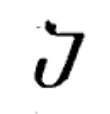
\includegraphics[scale=0.15]{images/georgianLetter.png}. See footnote \ref{footnote:georgian letter}. }} and it is found in the words in Table \ref{tab:Van:subdialect:Vozim:q}. I have not found this sound in other places.









\begin{table}[H]
	\centering
	\caption{Uvular stop /q/ <\armenian{ղՙ}> in the Vozim subdialect of the Van dialect}
	\label{tab:Van:subdialect:Vozim:q}
	\resizebox{\textwidth}{!}{%
	\begin{tabular}{|l|ll|ll|ll|}
		\hline & \multicolumn{2}{l|}{Classical Armenian}& \multicolumn{2}{l|}{> Vozim (Van) }& \multicolumn{2}{l|}{cf. SEA }
		\\
		`to bathe' &loɡɑnɑl & \armenian{լոգանալ} & loqɑnɑl & \armenian{լօղՙանալ} & loɡɑnɑl, loʁɑnɑl& \armenian{լոգանալ, լողանալ} \\
		`horse-radish' & boɫk & \armenian{բողկ} & bʰʏq & \armenian{բՙիւղ} & boχk & \armenian{բողկ} \\ 
		\hline
	\end{tabular}
}
\end{table} 

\subparagraph{Diphthong /œu̯/ <\armenian{էօւ}> }

The diphthong /œu̯/ <\armenian{էօւ}> is pronounced as a fast /œu/ <\armenian{էօու}>. I have found this word only in the word in Table \ref{tab:Van:subdialect:Vozim:œ}.


\begin{table}[H]
	\centering
	\caption{Words with the sound /œu̯/ <\armenian{էօւ}> in the Vozim subdialect of the Van dialect}
	\label{tab:Van:subdialect:Vozim:œ}
	\begin{tabular}{|l|ll|ll|ll|}
		\hline & \multicolumn{2}{l|}{Classical Armenian}& \multicolumn{2}{l|}{> Vozim (Van) }& \multicolumn{2}{l|}{cf. SEA }
		\\
		`fish' &d͡zukən & \armenian{ձուկն} & d͡zʰœu̯k & \armenian{ձՙէօւկ} & d͡zuk & \armenian{ձուկ} \\ 
		\hline
	\end{tabular}
	
\end{table} 

\subparagraph{Voiced aspirates}

Besides these, the subdialect of Vozim has the voiced aspirates /bʰ ɡʰ dʰ d͡zʰ d͡ʒʰ/ <\armenian{բՙ գՙ դՙ ձՙ ջՙ}>, which come from the Armenian voiced consonants. 

\begin{adjarianpage}\label{page:148}\end{adjarianpage}% should be 148

\paragraph{Sound changes}

There are many differences in sound changes. 

\subparagraph{Classical Armenian /o/ <\armenian{ո}>}

The Classical Armenian sound /o/ <\armenian{ո}> changes to /u/ <\armenian{ու}>, similar to the Moks subdialect (Table \ref{tab:Van:subdialect:Vozim:change:o:u}).


\begin{table}[H]
	\centering
	\caption{Change from Classical Armenian /o/ <\armenian{ո}> to /u/ <\armenian{ու}> in the Vozim subdialect of the Van dialect}
	\label{tab:Van:subdialect:Vozim:change:o:u}
	\resizebox{\textwidth}{!}{%
	\begin{tabular}{|l|ll|ll|ll|}
		\hline & \multicolumn{2}{l|}{Classical Armenian}& \multicolumn{2}{l|}{> Vozim (Van) }& \multicolumn{2}{l|}{cf. SEA }
		\\
		`ploughshare' &χopʰ & \armenian{խոփ} & χupʰ & \armenian{խուփ} & χopʰ & \armenian{խոփ} \\ 
		`leaven (CA);   & χəmoɾ & \armenian{խմոր} & χmuɾ & \armenian{խմուր} & χəmoɾ & \armenian{խմոր} \\ 
 dough (SEA)' & & & & & &  \\ 
		`bosom' & t͡sot͡sʰ & \armenian{ծոց}& t͡sut͡sʰ & \armenian{ծուց} & t͡sot͡sʰ & \armenian{ծոց} \\
		`hell' & dəʒoχkʰ & \armenian{դժոխք}& dʰʒuχkʰʲ & \armenian{դՙժուխքյ} & dəʒoχkʰ & \armenian{դժոխք} \\
		`frog' & ɡoɾt & \armenian{գորտ}& ɡʲoɾt & \armenian{գյուրտ} & ɡoɾt & \armenian{գորտ} \\
		`work' & ɡoɾt͡s & \armenian{գործ}& ɡʲuɾt͡s & \armenian{գյուրծ} & ɡoɾt͡s & \armenian{գործ} \\
		\hline
	\end{tabular}
}
\end{table} 



But this sound can also take the forms /ou̯, œ, ʏ, o/ <\armenian{օւ, էօ, իւ, օ}> (Table \ref{tab:Van:subdialect:Vozim:change:o:other}).


\begin{table}[H]
	\centering
	\caption{Change from Classical Armenian /o/ <\armenian{ո}> to /ou̯, œ, ʏ, o/ <\armenian{օւ, էօ, իւ, օ}> in the Vozim subdialect of the Van dialect}
	\label{tab:Van:subdialect:Vozim:change:o:other}
	\begin{tabular}{|l|ll|ll|ll|}
		\hline & \multicolumn{2}{l|}{Classical Armenian}& \multicolumn{2}{l|}{> Vozim (Van) }& \multicolumn{2}{l|}{cf. SEA }
		\\
		`mold' & boɾbos & \armenian{բորբոս}& bʰœɾbœs & \armenian{բՙէօրբէօս} & boɾbos & \armenian{բորբոս} \\
		`barefoot' & bokik & \armenian{բոկիկ}& bʰʏpek & \armenian{բՙիւպէկ} & bopik & \armenian{բոպիկ} \\
		`all' & boloɾ & \armenian{բոլոր}& bʰœlov & \armenian{բՙէօլօվ} & boloɾ & \armenian{բոլոր} \\
		`garlic' & səχtoɾ & \armenian{սխտոր}& səʁtou̯ɾ & \armenian{սըղտօւր} & səχtoɾ & \armenian{սխտոր} \\
		\hline
	\end{tabular}
	
\end{table} 

\subparagraph{Classical Armenian /iu̯/ <\armenian{իւ}>}

The Classical Armenian sound /iu̯/ <\armenian{իւ}> changes to /o, ou̯, e/ <\armenian{օ, օւ, է}> (Table \ref{tab:Van:subdialect:Vozim:change:iu}).


\begin{table}[H]
	\centering
	\caption{Change from Classical Armenian /iu̯/ <\armenian{իւ}> to /o, ou̯, e/ <\armenian{օ, օւ, է}> in the Vozim subdialect of the Van dialect}
	\label{tab:Van:subdialect:Vozim:change:iu}
	\begin{tabular}{|l|ll|ll|ll|}
		\hline & \multicolumn{2}{l|}{Classical Armenian}& \multicolumn{2}{l|}{> Vozim (Van) }& \multicolumn{2}{l|}{cf. SEA }
		\\
 
		`carpenter' & hiu̯sən & \armenian{հիւսն} & χou̯s & \armenian{խօւս} & hjusən & \armenian{հյուսն} \\ 
		`avalanche' & hiu̯s & \armenian{հիւս} & ou̯sĕi̯ & \armenian{օւսէʲ} & hjus & \armenian{հյուս} \\ 
		`bodkin' & heɾiu̯n & \armenian{հերիւն} & χĕi̯ɾon & \armenian{խէʲրօն} & heɾjun & \armenian{հերյուն} \\ 
		`hundred' & hɑɾiu̯ɾ & \armenian{հարիւր} & χɑɾeɾ & \armenian{խարէր} & hɑɾjuɾ & \armenian{հարյուր} \\
		`brick' & ɑɫiu̯s & \armenian{աղիւս}& oʁes & \armenian{օղէս} & ɑʁjus & \armenian{աղյուս} \\
		`flour' & ɑliu̯ɾ & \armenian{ալիւր} & jeloɾ & \armenian{յէլօր} & ɑljuɾ & \armenian{ալյուր} \\ 
		\hline
	\end{tabular}
	
\end{table}

\subparagraph{Classical Armenian /ɑi̯/ <\armenian{այ}>}

The Classical Armenian sound /ɑi̯/ <\armenian{այ}> changes not only to /e/ <\armenian{է}>, but also to /i̯e/ <\armenian{ե}> (Table \ref{tab:Van:subdialect:Vozim:change:e}).

\begin{table}[H]
	\centering
	\caption{Change from Classical Armenian /ɑi̯/ <\armenian{այ}> to /e, i̯e/ <\armenian{է, ե}> in the Vozim subdialect of the Van dialect}
	\label{tab:Van:subdialect:Vozim:change:e}
	\begin{tabular}{|l|ll|ll|ll|}
		\hline & \multicolumn{2}{l|}{Classical Armenian}& \multicolumn{2}{l|}{> Vozim (Van) }& \multicolumn{2}{l|}{cf. SEA }
		\\
		`vineyard' &ɑi̯ɡi& \armenian{այգի} & heɡe & \armenian{հէգէ} &ɑjɡi& \armenian{այգի} \\
		`goat' & ɑi̯t͡s & \armenian{այծ} & jet͡s & \armenian{յէծ} & ɑjt͡s & \armenian{այծ} \\ 
		`cave' &ɑi̯ɾ& \armenian{այր} & heɾ & \armenian{հէր} &ɑjɾ & \armenian{այր} \\
		`wide' & lɑi̯n & \armenian{լայն} & li̯en & \armenian{լեն} & lɑjn & \armenian{լայն} \\ 
		`father' & hɑi̯ɾ & \armenian{հայր} & χi̯eɾ & \armenian{խեր} & hɑjɾ & \armenian{հայր} \\ 
		`mother' & mɑi̯ɾ & \armenian{մայր} & mi̯eɾ & \armenian{մեր} & mɑjɾ & \armenian{մայր} \\ 
		\hline
	\end{tabular}
	
\end{table}

\subparagraph{Word-initial insertion of /h/ <\armenian{հ}> }
Words that start with a vowel often get an /h/ <\armenian{հ}> (Table \ref{tab:Van:subdialect:Vozim:change:h}).

\begin{table}[H]
	\centering
	\caption{Insertion of word-initial /h/ <\armenian{հ}> before Classical Armenian vowels in the Vozim subdialect of the Van dialect}
	\label{tab:Van:subdialect:Vozim:change:h}
	\resizebox{\textwidth}{!}{%
	\begin{tabular}{|l|ll|ll|ll|}
		\hline & \multicolumn{2}{l|}{Classical Armenian}& \multicolumn{2}{l|}{> Vozim (Van) }& \multicolumn{2}{l|}{cf. SEA }
		\\
		`durable' & ɑmuɾ & \armenian{ամուր} &hɑmuɾ & \armenian{համուր} & ɑmuɾ & \armenian{ամուր} \\ 
		`life (CA);    & ɑbɾɑnkʰ & \armenian{ապրանք} &hɑbɾɑnkʰ & \armenian{հաբրանք} & ɑbɾɑŋkʰ & \armenian{ապրանք} \\ 
 goods (SEA)' &  & & &  & &  \\ 
		`more' & ɑu̯eli & \armenian{աւելի} &hɑvil & \armenian{հավիլ} & ɑveli & \armenian{ավելի} \\ 
		`shore' & ɑpʰ & \armenian{ափ} &hɑpʰ & \armenian{հափ} & ɑpʰ & \armenian{ափ} \\ 
		`cheap' & ɑɾʒɑn & \armenian{արժան}& heʒɑn & \armenian{հէժան}& ɑɾʒɑn & \armenian{արժան} \\
		`oath' &eɾdumən & \armenian{երդումն} & heɾtou̯m & \armenian{հէրտօւմ} & jeɾtʰum & \armenian{երդում} \\ 
		`evening'& eɾekoi̯ & \armenian{երեկոյ} & heɾkon & \armenian{հէրկօն} & jeɾeko & \armenian{երեկո} \\
		\hline
	\end{tabular}
}
\end{table} 

\subsubsection{Morphology}

\paragraph{Noun inflection or declension}

In the declension of Vozim, it is noticeable that the genitive-dative uses the formatives /-ə, -ĕi̯/ <\armenian{ը, էʲն}>. The instrumental uses /-ov, -œv/ <\armenian{ով, էօվ}>. The plural uses /-dʰiɾ/ <\armenian{դՙիր}> (Table \ref{tab:Van:subdialect:Vozim:morpho:pl}).

\begin{table}[H]
	\centering
	\caption{Plural suffix /-dʰiɾ/ <\armenian{դՙիր}> in the Vozim subdialect of the Van dialect}
	\label{tab:Van:subdialect:Vozim:morpho:pl}
	\resizebox{\textwidth}{!}{%
	\begin{tabular}{|l|ll|ll|ll|}
		\hline & \multicolumn{2}{l|}{Classical Armenian}& \multicolumn{2}{l|}{> Vozim (Van) }& \multicolumn{2}{l|}{cf. SEA }
		\\
		`(male?) child' & təɫɑi̯ & \armenian{տղայ} & & & təʁɑ  & \armenian{տղա} \\
		`(male?) children' & təɫɑi̯-kʰ & \armenian{տղայք} & tʁejkʰ-dʰiɾ & \armenian{տղէյքդՙիր}& təʁɑ-kʰ & \armenian{տղաք} \\
		\hline
	\end{tabular}
}	
\end{table} 


The following is a small depiction of the case system (Table \ref{tab:Van:subdialect:Vozim:morpho:noun:decl}). 

\begin{table}[H]
	\centering
	\caption{Sample declension paradigm for a noun `bread'}\label{tab:Van:subdialect:Vozim:morpho:noun:decl}
	\begin{tabular}{|l| ll| ll |}
		\hline &\multicolumn{2}{l|}{Singular} &\multicolumn{2}{l|}{Plural} \\
		{\nom} & χɑt͡sʰ & \armenian{խաց} & χɑt͡sʰ-iɾ & \armenian{խացիր} \\
		{\gen}-{\dat} & χɑt͡sʰ-ə, χɑt͡sʰ-ĕi̯n & \armenian{խացը, խացէʲն} & χɑt͡sʰ-iɾ-u & \armenian{խացիրու} \\
		{\abl} & χɑt͡sʰ-en & \armenian{խացէն} & χɑt͡sʰ-iɾ-en & \armenian{խացիրէն} \\
		{\ins} & χɑt͡sʰ-u̯ov & \armenian{խացով} & χɑt͡sʰ-iɾ-u̯ov & \armenian{խացիրով}
		\\ \hline
	\end{tabular}
	
\end{table}

\paragraph{Pronoun inflection or declension}


The pronouns are the following (Tables \ref{tab:Van:subdialect:Vozim:morpho:pronoun:not3}, \ref{tab:Van:subdialect:Vozim:morpho:pronoun:3}). 

\begin{table}[H]
	\caption{Inflection paradigm for some (non-third person) personal pronouns in the Vozim subdialect of the Van dialect }\label{tab:Van:subdialect:Vozim:morpho:pronoun:not3}
	\centering 
		\resizebox{\textwidth}{!}{%
		\begin{tabular}{| l| llll| }
		\hline & 1SG & 2SG & 1PL & 2PL \\
		& `I' & `you' & `we'& `you' \\\hline 
		{\nom} & is & minkʰ & dʰu, dʰœ, dʰʏ & dʰœkʰ \\
		& \armenian{իս} & \armenian{մինք} & \armenian{դՙու, դՙէօ, դՙիւ} & \armenian{դՙէօք} \\\hline 
		{\gen} & im & mi & kʰʲʏ & d͡zʰ, d͡zʰə \\
		& \armenian{իմ} & \armenian{մի} & \armenian{քյիւ} & \armenian{ձՙի, ձՙը} \\\hline 
		{\dat} & d͡zej, ənd͡zej, d͡zi & mi & kʰʲi & d͡zʰi \\
		& \armenian{ձէյ, ընձէյ, ձի} & \armenian{մի} & \armenian{քյի} & \armenian{ձՙի} \\\hline 
		{\acc} & d͡zə, əzd͡zə & mi, zmi & kʰʲi, əzkʰʲi & d͡zʰi, əzd͡zʰi \\
		& \armenian{ձը, ըզձը} & \armenian{մի, զմի} & \armenian{քյի, ըզքյի} & \armenian{ձՙի, ըզձՙի} \\
		\hline {\abl} & ənd͡zne & mizne, mine & kʰʲine, kʰʲizne & d͡zʰine, d͡zʰizne \\
		& \armenian{ընձնէ} & \armenian{միզնէ, մինէ} & \armenian{քյինէ, քյիզնէ} & \armenian{ձՙինէ, ձՙիզնէ} \\
		\hline {\ins} & – & minu̯ov, miznu̯ov & kʰʲinu̯ov, kʰʲiznu̯ov & d͡zʰinu̯ov, d͡zʰiznu̯ov \\
		& – & \armenian{մինով, միզնով} & \armenian{քյինով, քյիզնով} & \armenian{ձՙինով, ձՙիզնով} \\
		& χɑd͡zej & χɑmi & χɑkʰʲi & χɑd͡zʰi \\
		& \armenian{խաձէյ} & \armenian{խամի} & \armenian{խաքյի} & \armenian{խաձՙի} 
		\\ \hline
	\end{tabular}
}
\end{table}


\begin{table}[H]
	\caption{Inflection paradigm for some (third person) personal pronouns in the Vozim subdialect of the Van dialect }\label{tab:Van:subdialect:Vozim:morpho:pronoun:3}
	\centering 
	\resizebox{\textwidth}{!}{%
	\begin{tabular}{| l| ll|ll| }
		\hline & 3SG & & 3PL & \\
		& `he' & & `they'& \\\hline 
		{\nom} & ɑn & \armenian{ան} & ɑnou̯nkʰ, nɑɾonkʰ & \armenian{անօւնք, նարօնք} \\
		{\gen}-{\dat} & ɑnou̯ɾ, nɑnou̯ɾ & \armenian{անօւր, նանօւր} & ɑnou̯nt͡sʰ, nɑnou̯nt͡sʰ & \armenian{անօւնց, նանօւնց} \\
		{\acc} & zɑnek & \armenian{զանէկ} & zɑnou̯nk & \armenian{զանօւնք} \\
		{\abl} & ɑnomne & \armenian{անօմնէ} & ɑnou̯nt͡sʰmne & \armenian{անօւնցմնէ} \\
		{\ins} & ɑnu̯of, ɑnu̯oχejt & \armenian{անոֆ, անոխէյտ} & ɑnou̯nt͡sʰ χejt & \armenian{անօւնց խէյտ} 
		\\ \hline
	\end{tabular}
}
\end{table}

\begin{adjarianpage}\label{page:149}\end{adjarianpage}% should be 149


At the edge of instrumentals, the form /χɑ/ <\armenian{խա}> is derived from the Classical word /het/ <\armenian{հետ}>, as can be guessed. Analogous to this is the Classical word /mɑu̯t/ <\armenian{մօտ}> `near', from which are formed the words in Table \ref{tab:Van:subdialect:Vozim:morpho:pron:ins}. 

\begin{table}[H]
	\centering
	\caption{Sample of instrumental pronouns (`near X') in the Vozim subdialect of the Van dialect}
	\label{tab:Van:subdialect:Vozim:morpho:pron:ins}
	\begin{tabular}{|l ll| }
		\hline 
		personal 1SG `near me' &mɑd͡zĕi̯ & \armenian{մաձէʲ} \\
		personal 1PL `near us' &mɑmi & \armenian{մամի} \\
		personal 2SG `near you' &mɑkʰʲi & \armenian{մաքյի} \\
		personal 2PL `near you' &mɑd͡zʰi & \armenian{մաձՙի} \\
		
		\hline 
	\end{tabular}
\end{table}

\subsubsection{Verb inflection or conjunction}

\paragraph{Overview and morphological changes}
\subparagraph{Theme vowel changes}
In conjugation, various changes occur, which are in accordance with phonetic rules. The present of the first conjugation takes the vowel /i/ <\armenian{ի}> vowel; while it takes /ĕi̯/ <\armenian{էʲ}> in the second conjugation. \translatorHD{He means that the Classical theme vowel /e/ became /i/, while the Classical theme vowel /i/ became /ĕi̯/. The original theme vowels are maintained in SWA (Table \ref{tab:Van:subdialect:Vozim:morpho:verb:themepast}). }

\subparagraph{Vowel hiatus between the theme vowel and the past suffix}

In the imperfective, the Classical sound sequence /ēi, ɑji/ <\armenian{էի, այի}> are changed to /e/ <\armenian{է}> (Table \ref{tab:Van:subdialect:Vozim:morpho:verb:themepast}). \translatorHD{To elaborate, when the theme vowel is before the past suffix, the two are replaced by a vowel /e/. It seems that this vowel /e/ marks the past tense. In contrast in SWA, the two vowel morphemes are separated by a glide /j/. }

\begin{table}[H]
	\centering
	\caption{Change from Classical Armenian theme vowels and past suffix in the Vozim subdialect of the Van dialect}
	\label{tab:Van:subdialect:Vozim:morpho:verb:themepast}
	\resizebox{\textwidth}{!}{%
	\begin{tabular}{|l|ll|ll|ll|}
		\hline & \multicolumn{2}{l|}{Classical Armenian}& \multicolumn{2}{l|}{> Vozim (Van) }& \multicolumn{2}{l|}{cf. SWA }
		\\\hline
		`I bring' & beɾ-e-m & \armenian{բերեմ} & kə bʰiɾ-i-m & \armenian{կը բՙիրիմ} & ɡə pʰeɾ-e-m & \armenian{կը բերեմ} \\ 
		`I speak' & χɑu̯s-i-m & \armenian{խօսիմ} & kə χos-ĕi̯-m & \armenian{կը խօսէʲմ} & ɡə χos-i-m & \armenian{կը խօսիմ} \\ 
		`I take' & tɑn-i-m & \armenian{տանիմ} & kə tɑn-ĕi̯-m & \armenian{կը տանէʲմ} & ɡə tɑn-i-m & \armenian{կը տանիմ} \\ 
		& \multicolumn{2}{l|}{$\sqrt{}$-{\thgloss}-1{\sg}}
		& \multicolumn{2}{l|}{{\ind} $\sqrt{}$-{\thgloss}-1{\sg}}
		& \multicolumn{2}{l|}{{\ind} $\sqrt{}$-{\thgloss}-1{\sg}}
		\\
		\hline 
		`I was crying' & l-ɑj-i-$\emptyset$ & \armenian{լայի} & k-il-$\emptyset$-e-$\emptyset$ & \armenian{կիլէ} & ɡu l-ɑj-i-$\emptyset$ & \armenian{կու լայի} \\ 
		`I was bringing' & beɾ-ē-i-$\emptyset$ & \armenian{բերէի} & kə bʰiɾ-$\emptyset$-e-$\emptyset$ & \armenian{կը բՙիրէ} & ɡə pʰeɾ-ej-i-$\emptyset$ & \armenian{կը բերէի} \\ 
		& \multicolumn{2}{l|}{$\sqrt{}$-{\thgloss}-{\pst}-1{\sg}}
		& \multicolumn{2}{l|}{{\ind} $\sqrt{}$-{\thgloss}-{\pst}-1{\sg}}
		& \multicolumn{2}{l|}{{\ind} $\sqrt{}$-{\thgloss}-{\pst}-1{\sg}}
		\\
		\hline 
		`I was' & jes ē-i-$\emptyset$ & \armenian{ես էի} &   is $\emptyset$-e-$\emptyset$ & \armenian{իս է} & jes ej-i-$\emptyset$ & \armenian{կու բերէի} \\ 
		& \multicolumn{2}{l|}{I {\aux}-{\pst}-1{\sg}}
		& \multicolumn{2}{l|}{I {\aux}-{\pst}-1{\sg}}
		& \multicolumn{2}{l|}{I {\aux}-{\pst}-1{\sg}}
		\\
		\hline
	\end{tabular}
}
\end{table} 



\subparagraph{Past suffix}

The perfective takes the vowel /ĕi̯/ <\armenian{էʲ}> (Table \ref{tab:Van:subdialect:Vozim:morpho:verb:pastperfective}). 

\begin{table}[H]
	\centering
	\caption{Change from Classical Armenian past perfective in the Vozim subdialect of the Van dialect}
	\label{tab:Van:subdialect:Vozim:morpho:verb:pastperfective}
	\begin{tabular}{|l|ll|ll|}
		\hline & \multicolumn{2}{l|}{Vozim (Van) }& \multicolumn{2}{l|}{cf. SWA }
		\\\hline
		`I called' & kɑnt͡ʃʰ-ə-t͡sʰ-ĕi̯-$\emptyset$ & \armenian{կանչըցէʲ} & ɡɑnt͡ʃʰ-e-t͡sʰ-i-$\emptyset$ & \armenian{կանչեցի} \\ 
		`I coughed' & χɑz-ɑ-t͡sʰ-ĕi̯-$\emptyset$ & \armenian{խազացէʲ} & hɑz-ɑ-t͡sʰ-i-$\emptyset$ & \armenian{հազացի} \\ 
		`I discussed' & zɾut͡sʰ-e-t͡sʰ-ĕi̯-$\emptyset$ & \armenian{զրուցէցէʲ} & zəɾut͡sʰ-e-t͡sʰ-i-$\emptyset$ & \armenian{զրուցեցի} \\ 
		& \multicolumn{2}{l|}{$\sqrt{}$-{\thgloss}-{\aor}-{\pst}-1{\sg}}
		& \multicolumn{2}{l|}{$\sqrt{}$-{\thgloss}-{\aor}-{\pst}-1{\sg}}
		\\
		\hline 
	\end{tabular}
	
\end{table} 

\subparagraph{Future marker}


The marker of the future is /tə/ <\armenian{տը}> (Table \ref{tab:Van:subdialect:Vozim:morpho:verb:fut}).

\begin{table}[H]
	\centering
	\caption{Future marker in the Vozim subdialect of the Van dialect}
	\label{tab:Van:subdialect:Vozim:morpho:verb:fut}
		\resizebox{\textwidth}{!}{%
		\begin{tabular}{|l|ll|ll|l|}
		\hline & \multicolumn{2}{l|}{Vozim (Van) }& \multicolumn{2}{l|}{cf. SWA } & 
		\\\hline
		`I will bring' & tə bʰiɾ-i-m & \armenian{տը բՙիրիմ} & bidi pʰeɾ-e-m & \armenian{պիտի բերեմ} & {{\fut} $\sqrt{}$-{\thgloss}-1{\sg}}
		\\ 
		`I was going to bring' & tə bʰiɾ-$\emptyset$-e-m & \armenian{տը բՙիրէ} & bidi pʰeɾ-ej-i-m & \armenian{պիտի բերէի} 
		&  {{\fut} $\sqrt{}$-{\thgloss}-{\pst}-1{\sg}}
		\\
		\hline 
	\end{tabular}
}
\end{table} 


\paragraph{General paradigms for the reflex of the E-Class}

The following is the conjugation of the Classical verb /uz-e-m/ <\armenian{ուզեմ}> `I want'. 



{\paradigmExplanation}

\subparagraph{Subjunctive present and past}

\translatorHD{In SWA, the subjunctive present is formed by adding agreement markers after the theme vowel. For a verb like /uz-e-l/ `to want', the theme vowel is an invariant /e/. In the Vozim subdialect of the Van dialect, essentially the same strategy is used with slightly different agreement markers. The theme for this verb in this context is /i/.}

\begin{table}[H]
	\centering
	\caption{Subjunctive present <\armenian{ստորադասական ներկայ}> of the verb `to want' in the Vozim subdialect of the Van dialect}
	\label{tab:Van:subdialect:Vozim:morpho:verb:paradigm:subjPresent}
	\begin{tabular}{|l|ll|ll|}
		\hline & \multicolumn{2}{l|}{Vozim (Van)} & \multicolumn{2}{l|}{cf. SWA} \\
		1SG & ou̯z-i-m & \armenian{օւզիմ} & uz-e-m & \armenian{ուզեմ} \\
		2SG & ou̯z-i-s & \armenian{օւզիս} & uz-e-s & \armenian{ուզես} \\
		3SG & ou̯z-i-$\emptyset$ & \armenian{ուզի} & uz-e-$\emptyset$ & \armenian{ուզէ} \\
		1PL & ou̯z-i-nkʰ & \armenian{օւզինք} & uz-e-ŋkʰ & \armenian{ուզենք} \\
		2PL & ou̯z-i-kʰ & \armenian{օւզիք} & uz-e-kʰ & \armenian{ուզէք} \\
		3PL & ou̯z-i-n & \armenian{օւզին} & uz-e-n & \armenian{ուզեն} \\
		& \multicolumn{2}{l|}{$\sqrt{}$-{\thgloss}-{\agr}}& \multicolumn{2}{l|}{$\sqrt{}$-{\thgloss}-{\agr}}\\ 
		
		\hline 
	\end{tabular}
\end{table}

\translatorHD{In SWA, the subjunctive past (Table \ref{tab:Van:subdialect:Vozim:morpho:verb:paradigm:subjPast}) is formed by adding the past suffix /i/ and agreement suffixes after the theme vowel. The past suffix is absent in the 3SG. In Vozim, the theme vowel is deleted before the past suffix /e/. Note that the 2SG and 3SG are homophonous with a final [eɾ], but the vowel  belongs to possibly different morphemes. }



\begin{table}[H]
	\centering
	\caption{Subjunctive past <\armenian{ստորադասական անցեալ}> of the verb `to want' in the Vozim subdialect of the Van dialect}
	\label{tab:Van:subdialect:Vozim:morpho:verb:paradigm:subjPast}
	\begin{tabular}{|l|ll|ll|}
		\hline & \multicolumn{2}{l|}{Vozim (Van)} & \multicolumn{2}{l|}{cf. SWA} \\
		1SG & ou̯z-$\emptyset$-e-$\emptyset$ & \armenian{օւզէ} & uz-ej-i-$\emptyset$ & \armenian{ուզէի} \\
		2SG & ou̯z-$\emptyset$-e-ɾ & \armenian{օւզէր} & uz-ej-i-ɾ & \armenian{ուզէիր} \\
		3SG & ou̯z-e-$\emptyset$-ɾ & \armenian{օւզէր} & uz-e-$\emptyset$-ɾ & \armenian{ուզէր} \\
		1PL & ou̯z-$\emptyset$-e-nkʰ & \armenian{օւզէնք} & uz-ej-i-ŋkʰ & \armenian{ուզէինք} \\
		2PL & ou̯z-$\emptyset$-e-kʰ & \armenian{օւզէք} & uz-ej-i-kʰ & \armenian{ուզէիք} \\
		3PL & ou̯z-$\emptyset$-e-n & \armenian{օւզէն} & uz-ej-i-n & \armenian{ուզէին} \\
		& \multicolumn{2}{l|}{$\sqrt{}$-{\thgloss}-{\pst}-{\agr}}& \multicolumn{2}{l|}{$\sqrt{}$-{\thgloss}-{\pst}-{\agr}}\\ 
		
		\hline 
	\end{tabular}
\end{table}


\subparagraph{Tenses built from the subjunctive: Indicative and future }

\translatorHD{In Vozim, many other tenses seem to be built off of the subjunctive (Table \ref{tab:Van:subdialect:Vozim:morpho:verb:paradigm:complexSubjunctive}). The indicative present and past imperfective are built by adding the prefix /k-/ before the subjunctive present and subjunctive past. The future and past future are formed also by adding the proclitic /piti/ before the appropriate subjunctive form. SWA behaves essentially the same and I don't provide its paradigm. }

\begin{table}[H]
	\centering
	\caption{Forms that are built from the subjunctive forms for the verb `to want' in the Vozim subdialect of the Van dialect}
	\label{tab:Van:subdialect:Vozim:morpho:verb:paradigm:complexSubjunctive}
	\resizebox{\textwidth}{!}{%
	\begin{tabular}{|l|ll|ll|}
		\hline & 
		\multicolumn{2}{l|}{Indicative present <\armenian{ներկայ}> } & \multicolumn{2}{l|}{Indicative past imperfective <\armenian{անկատար}>} \\
		1SG & k-ou̯z-i-m & \armenian{կօւզիմ} & k-ou̯z-$\emptyset$-e-$\emptyset$ & \armenian{կօւզէ} \\
		2SG & k-ou̯z-i-s & \armenian{կօւզիս} & k-ou̯z-$\emptyset$-e-ɾ & \armenian{կօւզէր} \\
		3SG & k-ou̯z-i-$\emptyset$ & \armenian{կօւզի} & k-ou̯z-e-$\emptyset$-ɾ & \armenian{կօւզէր} \\
		1PL & k-ou̯z-i-nkʰ & \armenian{կօւզինք} & k-ou̯z-$\emptyset$-e-nkʰ & \armenian{կօւզէնք} \\
		2PL & k-ou̯z-i-kʰ & \armenian{կօւզիք} & k-ou̯z-$\emptyset$-e-kʰ & \armenian{կօւզէք} \\
		3PL & k-ou̯z-i-n & \armenian{կօւզին} & k-ou̯z-$\emptyset$-e-n & \armenian{կօւզէն} 
		\\
		& \multicolumn{2}{l|}{{\ind}-$\sqrt{}$-{\thgloss}-{\agr}}& \multicolumn{2}{l|}{{\ind}-$\sqrt{}$-{\thgloss}-{\pst}-{\agr}}
		\\ \hline 
		& \multicolumn{2}{l|}{Future <\armenian{ապառնի}>} & \multicolumn{2}{l|}{Past future <\armenian{անցեալ ապառնի}> } \\
		1SG & t-ou̯z-i-m & \armenian{տօւզիմ} & t-ou̯z-$\emptyset$-e-$\emptyset$ & \armenian{տօւզէ} \\
		2SG & t-ou̯z-i-s & \armenian{տօւզիս} &t-ou̯z-$\emptyset$-e-ɾ & \armenian{տօւզէր} \\
		3SG &t-ou̯z-i-$\emptyset$ & \armenian{տօւզի} & t-ou̯z-e-$\emptyset$-ɾ & \armenian{տօւզէ} \\
		1PL & t-ou̯z-i-nkʰ & \armenian{տօւզինք} & t-ou̯z-$\emptyset$-e-nkʰ & \armenian{տօւզէնք} \\
		2PL & t-ou̯z-ikʰ & \armenian{տօւզիք} & t-ou̯z-$\emptyset$-e-kʰ & \armenian{տօւզէք} \\
		3PL & t-ou̯z-i-n &\armenian{տօւզին} & t-ou̯z-$\emptyset$-e-n & \armenian{տօւզէն} 
		\\
		& \multicolumn{2}{l|}{{\fut} $\sqrt{}$-{\thgloss}-{\agr}}& \multicolumn{2}{l|}{{\fut} $\sqrt{}$-{\thgloss}-{\pst}-{\agr}}
		\\\hline \end{tabular}
}
\end{table}

\subparagraph{Present perfect and past perfect}

\translatorHD{In SWA, the present perfect (Table \ref{tab:Van:subdialect:Vozim:morpho:verb:paradigm:presentPerfect}) and past perfect (Table \ref{tab:Van:subdialect:Vozim:morpho:verb:paradigm:pastPerfect}) are formed by combining a special non-finite form with the present/past auxiliary. For SWA, this non-finite verb can be either the resultative participle (verb with suffix /-ɑd͡z/) or the evidential participle (verb with suffix /-eɾ/). Vozim uses a similar system. The non-finite form is labeled as just a `past participle' by Adjarian (which I suspect is a perfective converb), and this form uses /-iɾ/ <\armenian{իր}>. }

\begin{table}[H]
	\centering
	\caption{Present perfect <\armenian{յարակատար}> of the verb `to want' in the Vozim subdialect of the Van dialect}
	\label{tab:Van:subdialect:Vozim:morpho:verb:paradigm:presentPerfect}
	\begin{tabular}{|l|ll|ll|}
		\hline & \multicolumn{2}{l|}{Vozim (Van)} & \multicolumn{2}{l|}{cf. SWA} \\
		1SG & ou̯z-iɾ i-m & \armenian{օւզիր իմ} & uz-eɾ e-m & \armenian{ուզեր եմ} \\
		2SG & ou̯z-iɾ i-s & \armenian{օւզիր իս} & uz-eɾ e-s & \armenian{ուզեր ես} \\
		3SG & ou̯z-iɾ i & \armenian{օւզիր ի} & uz-eɾ e & \armenian{ուզեր է} \\
		1PL & ou̯z-iɾ i-nkʰ & \armenian{օւզիր ինք} & uz-eɾ e-ŋkʰ & \armenian{ուզեր ենք} \\
		2PL & ou̯z-iɾ i-kʰ & \armenian{օւզիր իք} & uz-eɾ e-kʰ & \armenian{ուզեր էք} \\
		3PL & ou̯z-iɾ i-n & \armenian{օւզիր ին} & uz-eɾ e-n & \armenian{ուզեր են} \\
		& \multicolumn{2}{l|}{$\sqrt{}$-{\perfcvb} {\aux}-{\agr}}& \multicolumn{2}{l|}{$\sqrt{}$-{\eptcp} {\aux}-{\agr}}\\ 
		
		\hline 
	\end{tabular}
\end{table}


\begin{table}[H]
	\centering
	\caption{Past perfect <\armenian{գերակատար}> of the verb `to want' in the Vozim subdialect of the Van dialect}
	\label{tab:Van:subdialect:Vozim:morpho:verb:paradigm:pastPerfect}
	\begin{tabular}{|l|ll|ll| }
		\hline & \multicolumn{2}{l|}{Vozim (Van)} & \multicolumn{2}{l|}{cf. SWA} \\
		1SG & ou̯z-iɾ $\emptyset$-e-$\emptyset$ & \armenian{ուզիր է} & uz-eɾ ej-i-$\emptyset$ & \armenian{ուզեր էի} \\
		2SG & ou̯z-iɾ $\emptyset$-e-ɾ & \armenian{ուզիր էր} & uz-eɾ ej-i-ɾ & \armenian{ուզեր էիր} \\
		3SG & ou̯z-iɾ e-$\emptyset$-ɾ & \armenian{ուզիր էր} & uz-eɾ e-$\emptyset$-ɾ & \armenian{ուզեր էր} \\
		1PL & ou̯z-iɾ $\emptyset$-e-nkʰ & \armenian{ուզիր էնք} & uz-eɾ ej-i-ŋkʰ & \armenian{ուզեր էինք} \\
		2PL & ou̯z-iɾ $\emptyset$-e-kʰ & \armenian{ուզիր էք} & uz-eɾ ej-i-kʰ & \armenian{ուզեր էիք} \\
		3PL & ou̯z-iɾ $\emptyset$-e-n & \armenian{ուզիր էն} & uz-eɾ ej-i-n & \armenian{ուզեր էին} \\
		& \multicolumn{2}{l|}{$\sqrt{}$-{\perfcvb} {\aux}-{\pst}-{\agr}}& \multicolumn{2}{l|}{$\sqrt{}$-{\eptcp} {\aux}-{\pst}-{\agr}}\\ 
		
		\hline 
	\end{tabular}
\end{table}


\subparagraph{Past perfective or aorist}\label{sec:Van:subdialect:vozim:verb:paradigm:pastperf}

\translatorHD{The past perfective (Table \ref{tab:Van:subdialect:Vozim:morpho:verb:paradigm:pastperfectiveAorist}) is also called the aorist. In SWA for /uz-e-l/ `to want', the past perfective is formed by taking the root and theme vowel, adding the aorist or perfective suffix /-t͡sʰ-/, and then adding the past suffix /-i/ and the appropriate agreement suffixes. The 3SG uses covert tense and agreement suffixes. The Vozim subdialect behaves the same, though the past suffix is /-ej/ and the theme vowel is /e/ in all but the 3SG. Note that in Adjarian's earlier transcriptions, he said the past suffix is /ĕi̯/ <\armenian{էʲ}> but his paradigm uses /ej/ <\armenian{էյ}>. }


\begin{table}[H]
	\centering
	\caption{Past perfective or aorist <\armenian{կատարեալ}> of the verb `to want' in the Vozim subdialect of the Van dialect}
	\label{tab:Van:subdialect:Vozim:morpho:verb:paradigm:pastperfectiveAorist}
	\begin{tabular}{|l|ll|ll|}
		\hline & \multicolumn{2}{l|}{Vozim (Van)} & \multicolumn{2}{l|}{cf. SWA} \\
		1SG & ou̯z-e-t͡sʰ-ej-$\emptyset$ & \armenian{օւզէցէյ} & uz-e-t͡sʰ-i-$\emptyset$ & \armenian{ուզեցի} \\
		2SG & ou̯z-e-t͡sʰ-ej-ɾ & \armenian{օւզէցէյր} & uz-e-t͡sʰ-i-ɾ & \armenian{ուզեցիր} \\
		3SG & ou̯z-i-t͡sʰ-$\emptyset$-$\emptyset$ & \armenian{օւզից} & uz-e-t͡sʰ-$\emptyset$-$\emptyset$ & \armenian{ուզեց} \\
		1PL & ou̯z-e-t͡sʰ-ej-ŋkʰ & \armenian{օւզէցէյնք} & uz-e-t͡sʰ-i-ŋkʰ & \armenian{ուզեցինք} \\
		2PL & ou̯z-e-t͡sʰ-ej-kʰ & \armenian{օւզէցէյք} & uz-e-t͡sʰ-i-kʰ & \armenian{ուզեցիք} \\
		3PL & ou̯z-e-t͡sʰ-ej-n & \armenian{օւզէցէյն} & uz-e-t͡sʰ-i-n & \armenian{ուզեցին} \\
		& \multicolumn{2}{l|}{$\sqrt{}$-{\thgloss}-{\aor}-{\pst}-{\agr}}& \multicolumn{2}{l|}{$\sqrt{}$-{\thgloss}-{\aor}-{\pst}-{\agr}}\\ 
		
		\hline 
	\end{tabular}
\end{table}
\subparagraph{Imperative and prohibitive}\label{sec:Van:morphology:verb:paradigm:imp}

\translatorHD{For the imperative 2SG, SWA adds a zero morph /-$\emptyset$/ after the theme vowel /e/ for a verb like `to want' (Table \ref{tab:Van:subdialect:Vozim:morpho:verb:paradigm:Imp}). For the 2PL, SWA adds the sequence /-e-t͡sʰ-ekʰ/ after the root such that /-e-t͡sʰ/ forms the aorist stem, while /-ekʰ/ is the agreement marker. Vozim instead adds a vowel /i/ for the 2SG; it's unclear if this /i/ is the theme vowel or an added suffix. For the 2PL, the suffix /ekʰ/ is added after the aorist stem. }


\begin{table}[H]
	\centering
	\caption{Imperative forms <\armenian{հրամայական}> for the verb `to want' in the Vozim subdialect of the Van dialect}
	\label{tab:Van:subdialect:Vozim:morpho:verb:paradigm:Imp}
	\resizebox{\textwidth}{!}{%
	\begin{tabular}{|l|lll|ll l|}
		\hline & \multicolumn{3}{l|}{Vozim (Van)} & \multicolumn{3}{l|}{cf. SWA} \\
		2SG & ou̯z-\'i & \armenian{օւզի՛} & $\sqrt{}$-?& uz-e-$\emptyset$ & \armenian{ուզէ՛} & $\sqrt{}$-{\thgloss}-{\imp}.2{\sg}
		\\
		2PL& ou̯z-e-t͡sʰ-ekʰ& \armenian{օւզէցէք} & $\sqrt{}$-{\thgloss}-{\aor}-{\imp}.2{\pl}& uz-e-t͡sʰ-ekʰ& \armenian{ուզեցէք} & $\sqrt{}$-{\thgloss}-{\aor}-{\imp}.2{\pl}
		\\\hline \end{tabular}
}
\end{table}

\translatorHD{For the prohibitive or negative imperative (Table \ref{tab:Van:subdialect:Vozim:morpho:verb:paradigm:Proh}), SWA adds the prohibitive formative /mi/ before the verb. The verb takes a suffix /-ɾ/ in the 2SG, and /-kʰ/ in the 2PL. In Vozim, the prohibitive is made up of the prefix /m-/ plus the imperative verb. } 


\begin{table}[H]
	\centering
	\caption{Negative imperative or prohibitive forms for the verb `to want' in the Vozim subdialect of the Van dialect}
	\label{tab:Van:subdialect:Vozim:morpho:verb:paradigm:Proh}
	\resizebox{\textwidth}{!}{%
	\begin{tabular}{|l|lll|lll|}
		\hline & \multicolumn{3}{l|}{Vozim (Van)} & \multicolumn{3}{l|}{cf. SWA} \\
		2SG & m-\'ou̯z-i̯ & \armenian{մօ՛ւզի} & {\proh}-$\sqrt{}$-? & m\'i uz-e-ɾ & \armenian{մի ուզեր} & {\proh} $\sqrt{}$-{\thgloss}-2{\sg} \\
		2PL & m-\'ou̯z-e-t͡sʰ-ekʰ & \armenian{մօ՛ւզէցէք} & {\proh}-$\sqrt{}$-{\thgloss}-{\aor}-{\imp}.2{\pl} & m\'i uz-ekʰ& \armenian{մի ուզէք} & {\proh} $\sqrt{}$-{\thgloss}-2{\pl} \\
		\hline \end{tabular}
}
\end{table}

\translatorHD{On page \ref{page:157}, Adjarian left a footnote with examples of imperatives and prohibitives from Vozim (Table \ref{tab:Van:lit:Vozim:imp}), sentence}. 

\begin{table}[H]
	\centering
	\caption{Imperatives and prohibitives in the Vozim subdialect of the Van dialect}
	\label{tab:Van:lit:Vozim:imp}
	\begin{tabular}{|l|ll|ll|}
		\hline & \multicolumn{2}{l|}{Vozim (Van)}& \multicolumn{2}{l|}{cf. SWA }
		\\
		`bring! ({\sg})' & bʰi & \armenian{բՙի} & pʰeɾ& \armenian{բեր} \\
		`put! ({\sg})' & dʰi & \armenian{դՙի} & tʰiɾ& \armenian{դիր} \\
		`eat! ({\sg})' & ki & \armenian{կի} & ɡeɾ& \armenian{կեր} \\
		`don't eat! ({\sg})' & mou̯ti & \armenian{մ՚օւտի} & mi uteɾ& \armenian{մի՛ ուտեր} \\
		\hline
	\end{tabular}
	
\end{table}

\begin{exe} 
	\ex Vozim (Van) dialect \\
	\gll bʰi dʰi mɑ d͡zi, ki χɑ d͡zi \\
	bring.{\imp}.2{\sg} put.{\imp}.2{\sg} near me.{\dat}, eat.{\imp}.2{\sg} with me.{\dat}\\
	\trans `Come bring it near me, eat with me.' \\
	\armenian{բՙի դՙի մա ձի, կի խա ձի}
\end{exe}

\subparagraph{Non-finite forms}

\translatorHD{Finally, Adjarian lists the following non-finite forms of this verb (participles or converbs) in Table \ref{tab:Van:subdialect:Vozim:morpho:verb:paradigm:participle}. I give SWA forms for just some of them because it's unclear to me what these Vozim participles mean. Note that Adjarian uses the term `past participle' to mean multiple different types of non-finite forms: resultative participle with /-ɑd͡z/ in SWA, evidential participle /-eɾ/ in SWA. I suspect the Vozim /-iɾ/ is a perfective converb. } 

\begin{table}[H]
	\centering
	\caption{Participles or converbs <\armenian{դերբայներ}> for the verb `to want' in the Vozim subdialect of the Van dialect}
	\label{tab:Van:subdialect:Vozim:morpho:verb:paradigm:participle}
		\resizebox{\textwidth}{!}{%
		\begin{tabular}{|ll|lll|lll|}
		\hline & & \multicolumn{3}{l|}{Vozim (Van)} & \multicolumn{3}{l|}{cf. SWA} \\
		Infinitive & \armenian{անորոշ} & ou̯z-i-l & \armenian{օւզիլ} & $\sqrt{}$-{\thgloss}-{\infgloss} & uz-e-l & \armenian{ուզել} & $\sqrt{}$-{\thgloss}-{\infgloss} \\
		Past & \armenian{անցեալ} & ou̯z-ɑt͡s & \armenian{օւզած} & $\sqrt{}$-{\rptcp} & uz-ɑd͡z & \armenian{ուզած} & $\sqrt{}$-{\rptcp} \\
		& & o̯uz-iɾ & \armenian{օւզիր}& $\sqrt{}$-{\perfcvb} & uz-eɾ & \armenian{ուզեր}& $\sqrt{}$-{\eptcp} \\
		Future & \armenian{ապառնի} & o̯uz-i-l-ʏ & \armenian{օւզիլիւ} & $\sqrt{}$-{\thgloss}-{\infgloss}-{\futcvb} & uz-e-l-u & \armenian{ուզելու} & $\sqrt{}$-{\thgloss}-{\infgloss}-{\futcvb} \\
		\hline \end{tabular}
}
\end{table}

\begin{adjarianpage}\label{page:150}\end{adjarianpage}% should be 150

\section{Literature}

The first study on the Van dialect was done by someone named \armenian{Գրիչ} (see \armenian{Փորձ. Ա}. number 2, page 339-358)\footnote{\translatorHD{I couldn't track down this reference. The word \armenian{Գրիչ} (SEA: /ɡəɾit͡ʃʰ/) is the Armenian word for `pen', which makes me think this was an anonymous entry.}} during a study of `Manna' \citep{manana} by Garegin Srvandztiants (\armenian{Գ. Վ. Սրուանձտեան}; \translatorHD{SEA: /səɾvɑnd͡ztjɑn/, SWA: /səɾvɑnt͡sʰtjɑn/}). The second and last work was my work in German \citep{adjarian-1901-lautlehreVan}. This contains a detailed phonology of the Van dialect, done with European scientific transliteration. 

{\litoverview}

\begin{itemize}
	\item Literature with the Van dialect
	\begin{itemize}
		\item General Van dialect:
		\begin{itemize}
			\item \armenian{Արիստ. Վ. Տէր-Սարգսեան – Պանդուխտ Վանցին. Պօլիս}, 1875
			\item \armenian{Արիստ. Վ. Սեդրակեան – Քնար Մշեցոց եւ Վանեցոց. Վղրշպտ}. 1874
			\item \armenian{Գէորգ Շէրենց – Վանայ Սազ. Թիֆլիս, Ա}. 1886, \armenian{Բ}. 1899
			\item \armenian{Գ. Վ. Սրուանձտեանց} 
			\begin{itemize}
				\item 
				– \armenian{Գրոց ու բրոց. Պօլիս}. 1874
				\item – \armenian{Մանանայ. Պօլիս}. 1876
				\item – \armenian{Համով հոտով. Պօլիս}.
			\end{itemize}
			\item \armenian{Տիգրան Տէրոյեան – Երգարան. Պոսթոն}. 1901, page 549-592
			\item \armenian{Գրիչ – Պանդուխտ Վանցին}. (\armenian{Մատենախ}). \armenian{Փորձ. Ա. թ}. 3, \armenian{էջ} 113-135
			
		\end{itemize}
		\item Moks subdialect
		\begin{itemize}
			\item \armenian{Գարեգին Սարկաւագ – Սասմայ ծռեր. Թիֆլիս}. 1892, page 61-151
			\item \armenian{Գ. Վ. Յովսէփեան – Ռոստամ Զալ. Ազգ. Հանդ. Է. էջ} 205-254
			
			\begin{adjarianpage}\label{page:151}\end{adjarianpage}% should be 151
			
			\item \armenian{Բ. Խալաթեանց – Իրանի հերոսները. Պարիզ}, 1901, \armenian{էջ} 45-56
			\item \armenian{Ա. Աբեղեան – Թլուատ Դաւիթ. Թիֆլիս} 1902
			\item \armenian{Մ. Աբեղեան – Դաւիթ եւ Մհեր. Շուշի} 1889
			\item \armenian{Հայ-Արմէն – Մոկաց երգեր. Արեւել. մամուլ}. 1890, \armenian{էջ} 177-179
			
			
		\end{itemize}
		\item Besides these, Sarkis Haykuni (\armenian{Ս. Հայկունի}) has published 34 fables from Van, Moks, Norduz, Shatakh, and Vozim. See \citetitle{Eminian}, \armenian{Վղրշպտ}. volume 2 and 4-6 (\armenian{Բ, Դ-Զ}). 
		\item There are a number of small manuscripts in the \citetitle{Byurakn} periodical. 
		\begin{itemize}
			\item From Van – 1898, \armenian{էջ} 183, 459, 558, 583, 1899, \armenian{էջ} 15, 151
			\item Shatakh – 1898, \armenian{էջ} 558, 569
			\item from Vozim – 1899, \armenian{էջ} 20, 119, 298
			
		\end{itemize}
		
	\end{itemize}
\end{itemize}


\section{Text samples}

{\sampleoverview}

\subsection{Van dialect }

Adjarian's source: I have taken from \armenian{Տէր-Սարգսեանցի Պանդուխտ Վանցի}, page 52-55, changing it to my orthography. 

\armenian{Էս քյանի տարի ի կուկյա̈ ու կընցնի. էս քյանի տարի ի մեր աչք քյո ճա̈մխի վէրէն կը խալի. էս քյանի տարի ի մեր սիռտ քյե խամար կը մաշվի. էս քյանի տարի ի քյո սիրուց կը մյանքյ կարօտ. է՜հ, վո՞վ իմ յարալու սիռտ պիրէր չիւմ քյո մօտ, վոր պա̈նիր տիսնիր ինոր ցավեր ու վէրքեր։ Ա՜հ, չանձ հըմէն կսկծավոր յես եմ վիրավոր, չանձ հըմէն խռօված յես եմ տրօրված, իրիցած ու մրկած։}

\armenian{Թօղ կյա̈րիւն կյա̈}. \armenian{էրկիր, սարերն ու տա̈ղտեր կանաչ, կարմիր ու նարընջի զա̈րտըրի. ա՜խ, յես ի՞նչ անեմ ինոնքյ. յես մնացի ատնէր ու կյերի. յես մնացի վոռպէօվէրի։}

\armenian{Թօղ ամըռվան պտուղներ խասնեն, միլաղներաց պէս շարվին ու կաթիւկ անեն վեր կանաչ խոտին, լղմոր լղմոր լըղպորվին, յես ի՜նչ անեմ ինոնքյ, կարօտ մնացինքյ. տիւ պէտք ես խամ տաս ինոնց ու խոտ տաս, հա̈մ ինոնց, հա̈մ ձիկ։}

\armenian{Թօղ խօջան ժօղվէ առծաթն ու վոսկին, ակն պավական, միւջաֆարներ անգյին, չանձ Վա̈նա̈ ծով լիցուցի, չանձ աշխըրքիս սարեր բա̈րդի, թեղի ու սեխչի, ինոնքյ հըմէն առանց սիրու, առանց սռտի ինչի՞ս խամար ի. ա՜հ, առանց քյե աստըվորիս մալն յես ի՞նչ անեմ։ Ա՜խ, թէ յես քյե խամար մեռած եմ, էլմ՚ կասեմ, աշխերքիս մալն յես ի՞նչ անեմ։}


\begin{adjarianpage}\label{page:152}\end{adjarianpage}% should be 152

\armenian{Մենքյ ծեռքյ տվինքյ ծեռաց, ուխտ արինքյ խտրաց, վոր խտրաց ապրին, խտրաց մեռնինքյ. քյո սէր տվիր, իմ սիռտն առիր ու մեր սիրու խօսք լսեց էրկինքյ, լսեց էրկիր. մենքյ ուխտ արինքյ, ու մէմէկու վէրէն խոկյի կու տինքյ. ա՜հ, ճղակտոր էլա̈վ մեր յէղունիկ սէր. ու քյէօքյախան էլա̈վ մեր սիռտ. տիւ կարիբ կնա̈ցիր ու ինգյա̈ր օտար էրկիր ու զատ մնացիր. տիւ քյըռտինքյ կը թա̈փես, յես առտսունքյ. տիւ մէօլրած ես, յես բէզըրած, օրս աստըվորս կնա̈ց, էլ զադ չմնաց։ Էնչա̈նք կանչեմ, սարեր լացուցեմ, յես առանց քյե սէրն ի՞նչ անեմ, սիռտն ի՞նչ անեմ, ուխտն ի՞նչ անեմ, կյանքն ի՞նչ անեմ։}

\armenian{Քյո ջուխտակ այվընիկ ծա̈քյեր կուց կուց առտսունքյ կը թա̈փեն, կուլա̈ն ու կասեն. «Մեր խէրն ինչի՞ չիրե, դէդէ մարէ, ապա յեփ պիտի կյա̈»։ Ձի կը խառցուցեն, սիռտս կը դաղեն. էլ ինոնց խապելու մա̈ֆա̈ր չմնաց. ասքն ու պարիկամ տիւր տրացին, ձի խառցմունք կ՚անեն ծեր մարթուց ի՞նչ խա̈բա̈ր կա. յե՞փ պիտի կյա̈}. \armenian{էլ խէրիքյ չէլա̈վ կարիբութան մէջ մնա. էլ խոկյիս էլա̈վ շատերաց սուտ խապելուց. յես ծեռքյից կնա̈ցի։ Տիւրր տրացին, ասքն ու խնամին յես ի՞նչ անեմ առանց իմ ծէտկիկ ծա̈քյերու աղին. յես ի՞նչ անեմ վորտին, առանց իմ նաղէլի կարիբին. աշխար ձի մութ ի, վո՞վ կիրիշկի վեր լաճերաց, կարիբիս մեռնեմ ուր ճամխըներաց։}

\armenian{Մեր տուն տեղ մեր ծեռքյից էլա̈վ. օտար խաֆքյու պէս մնացինք վեր չոր խըլի. վո՞վ պիտի մեր նեղութեն տիսնա, մեզ օղօրմի. խեխճ ու անտէր մնացինքյ. քյեղնից տվել մարթ չունինքյ. ի՞նչ կասես, սաղ սաղ մեռնե՞նքյ։}

\armenian{Խէրտ ու մէրտ խալիվորցիր են. յես ինոնց դարդն չեմ կանա քյաշե. յես քյե քիչ կյըրիցի, տիւ շատ իմացի. շոտ թօղ արե, էլ խէրիքյ ի. խէրիքյ ի տա̈ռն տա̈տէք, տա̈ռտակ նստէքյ. իսկի չէ տարին քյանի մ՚ կուռուշ փարա ճամխէքյ. մենքյ էրթա̈նքյ մուրանքյ, պիրենքյ քյո տղէյնե՞ր պախենքյ. էլ չենքյ կանա անել, ինչ վոր արինքյ՝ էն էլ խէրիքյ ի։}

\subsection{Diyadin subdialect}

Adjarian's source: From the village of Basargechar of New Bayazet. 

\armenian{Իմ խէր իմ ախպօր խէտ մէ օր առանց սէլ քյնացին (կամ քյացին) վոր քիւլա̈շ բերեն. քյամին կայնավ. շատ էլ քյամի էր}... 



\begin{adjarianpage}\label{page:153}\end{adjarianpage}% should be 153

... \armenian{ինչքյան սէլ բա̈րցին, քյամին խըրցներ վէր տըվեց, քըցեց քյետին. չուր էնի կառնի կը դնի, քյամին վէր կուտա։ Խէրս յերսօտ էր. քյամու վրէն յէրսօտավ, խըրցներ վէր տըվեց ասեց. էս էլ քյեզ, էս էլ քյեզ։ Փափախն էլ կը խանա կը ղլօդկա կը քըցա գյեսին. շորերն էլ վրէվէն խանեց քցեց. էս էլ քյեզ. խօ չէս ի քյա էս էլ պրծուս տանես։}


\begin{center}
	* *
\end{center}

\armenian{Զատկի խլուսուն էր. էկան իմ ախչկէն ուզելու. խէրն էլ ասաց իմ ախչիկ կուտամ քյօ տղին։ ուրանք լավ ին. ուրանց բնուեն լավ էր, ամա քյասիբ ին. է՛հ, ուր կընկյան կը պախա ասինքյ տըվեցինք. ամա ախչկա սրտօվ չէր։ Մնաց վոր իմ տղէք գիտին (գիտցած ին) թէ իմ մարթ թռանա (հանաք, կատակ) էրեր ա ուրանց խետ, թէ իմ ախչիկ կուտամ քյօ տղին. չին գիտցե վոր սրտանց էր ասեր էր. վոր յետօ իմացան թէ էս բա̈ն օղորթ ա, ուզեցան քրոչ թէ առի (արի) յետ դա̈ռի, մի՛ առնի։ Ախչիկ լէ վէրցրեց թէ յես հարուստ մարթու ախչիկ ըլնեմ, իմ բիւլոր ախբՙրներու անուն ափեմ գյետի՞ն։ Յետօ յեխբՙարներ կայնան թէ արի քյեզի յետ դարցուցենքյ, էլ չենքյ իտա էն տղին, լավ տղի կուտանքյ։ Իւր քիւր վէրցրեց թէ յեխբՙար ջանէ, չե՛ղի դառնալ. իմ խօր անվանի ամօթ ա։ Ուր անուն լէ Սօֆյան ա։}

\armenian{Մէ ամըսվա խարս էլավ. լավ խարսնիս էրէցինքյ. խարսնըսէն մէ ամիս յետօ մախացավ. խինգյ օր խիվընդցավ մէռավ։ Յէս կանիծի կասի. բօխչէդ կապոկ մնա. խինէդ քյամին տանա. սկի արժան չըլնես վոր դու ընէնց խօնար չես էղե. կ՚ասէր. մա՛յրիկ ջանէ, ա՛դէ ջանէ, յես մկա մեռնիմ վոր քի՞չ լա̈ս, էն վախտ կը մեռնիմ վոր օխտը ձեռքի շոր էլնի, վոր դնես հառէչդ իմ խամար լա̈ս։}

\armenian{Մկա իմ տան էրէխէք վրէն խաղ ա կապած}.

\armenian{Յէս Սօփին եմ ծամավոր},

\armenian{Դու Մանուկն իր խամավոր}.

* * 


\armenian{Ղօրթմա (ճիշտ որ) խամավոր տղա էր. ամա քյասիբ էր. քյասիբին գինաս ի՛նչ ղդար պատվելի էլնի, ինչքյան լավ զրուցա, պատիվ չկա. քյասբի բա̈ն մերժուկ ա։}

\armenian{Մկա կիւլա̈մ. օր իրեքյ խետ կիւլա̈մ. բա չե՞մ իլա̈}. \armenian{էն շորեր վոր կարի, վոչ խաքյավ. ինչ վոր կարի՝ կապուկ մնաց. մկա}... 


\begin{adjarianpage}\label{page:154}\end{adjarianpage}% should be 154

... \armenian{կանիծե՞մ. էն վախտ կանիծի. իմ լիզուն չորնէր. մկա չեմ անիծե, յ̵ախու չեմ անիծե։}

\armenian{Քյօ դախին է՞տ էր. կըսա արթանքյ արթանքյ. մկա պրծա՞ր։}

Adjarian's source: This is narrated by the unfortunate mother of Sopia (\armenian{Սոփիա}), Aslik (\armenian{Ասլիկ}). I transcribed it during my summer travels of 1907 in Basargechar. 

\subsection{Moks subdialect}
Adjarian's source: See \citetitle{Eminian}, 4, page 57. 

\armenian{Թաքյավուր մ՚ կէր, իրիք տղա ուներ, իրիք ախչըկ. էսաց}. – \armenian{Իս կը միռնիմ, խաֆք գյա, գէլ գյա, առչ գյա, ախչկըտիր կըտէք (կուտաք}), \armenian{էսաց. իս ինչ կը միռնիմ, իմ իտիվէն չգէք՝ էսաց. ինչ կը պսակվէք՝ մա ձի կընկտիք չը քընէք՝ էսաց. ծառ մը կա մի (մենք ծառ մը ունինք}), \armenian{իրիք խնձուր կը բռնը. Հուլիսի տասնըխնգին կը գյան, կը տանը՛ն. չըն թուղնը տըսնանք ինչ խնձուր ի (անմահական խնձուր ի}). \armenian{ան ցածրի խնձուր մինծ տղըն, ան միչի խնձուր միչնիկ տղըն, ան վէրի խնձուրն էլ պզտը տղըն։ Էսաց. յօթ օր իմ գիրիզման կը պախէք. գըշիր ճրաքն էլ չըք թուղնը ընցնը։}

\armenian{Խէր միռավ. տը տանին վիրուցին. էրկու միծ տղէք ասըցըն}. – \armenian{Խիտ էրթանք։}

\armenian{Փուքր էսաց}. – \armenian{Չընք էրթա։}

– \armenian{Ի՞նչըխ, մի խէր մէռնը, ասըցըն, մինք չէրթա՞նք խիտ՝}

\armenian{Պզտիկ ախբէրն էլ առըն. զիւրովէն գնացըն խիտ։}

\armenian{Մինչիվ զխէր պախըցըն, էկան, խրօխբէր նստավ թախտ, թաքյավուրութեն առըց։}

\armenian{Փուքր ախբէր էսաց}. – \armenian{Չէ՞ իս ձի ասըցը «չինք էրթա իտիվ»։}

\armenian{Առչ իրի. նստավ խնամաթոռ}. – \armenian{Ձի մինծ քիւր տը տէք ձը, էսաց։}

\armenian{Էրկու մինծ ախբէր ասըցըն}. – \armenian{Մինք մի քիւր ի՞նչըխ տը տանք առչին. չընք իտա. տանը տ՚ուտէ։}

\armenian{Պզտիկ ախբէրն էսաց}. – \armenian{Իմ խօր խուսք չէրի, կուշտ կիրա. ա՛ս էլ չէնըմ, տը տամ տանը՛ (պիտի տամ տանի)։}

\armenian{Մինջ քիւր առչ առըց տարախ։}

\begin{adjarianpage}\label{page:155}\end{adjarianpage}% should be 155

\subsection{Norduz}


Adjarian's source: See \citetitle{Eminian}, 4, page 97. 

\armenian{Մէկ լավ տղէ-մ կէր. զինքն էր, ուր մէր. էլավ գնաց մէկ գեղ. ասաց}. – \armenian{Տ՚էհամ մօ ռէս, ըլնեմ վօրթկարած։}

\armenian{Գնաց, խնդրվավ, ասաց}. – \armenian{Ձի անես վօրթկարած, շախվեմ։}

\armenian{Ասաց}. – \armenian{Ա՛յ տղա, դիւ կանա՞ս վօրթիկներ շախես։ Ասաց}. – \armenian{Կանամ։}

\armenian{Ասաց. Դէ՛, գնա՛ յ̵էռչէվ վօրթկներաց. կիրակնեց կիրակի քիւ խաց-մաց ժօղվի յ̵ըմէն վօրթկի մէկ դիտր ցօրեն տամքիւ հախ։}

\armenian{Էլավ, գնաց յ̵էռչէվ վօրթկներաց։ Էն վօրթիկ իշ կը դըռչըկէր, պառաի կէհէր, էն կըհէր. տղէն կըհէր կը տփէր, բիրէր մըչ վօրթկներաց. իշ կը մնէր դումահիք (ետեւէն}), \armenian{կը տփէր, չում կը խասցնէր վօրթկներաց։}

\armenian{Էդա լավնով մէկ շարթվան մէչ խինք, վեց վօրթիկ սպանեց։} 

\armenian{Գէղական էլան, գնացին ռէսին ասին}.

– \armenian{Մենք էն վօրթկարած կապուլ չընք անի. մե վօրթկներ յ̵ըմէն սպանեց։}

\armenian{յ̵էլան մլուցին դիւս, գեղից խանին։}


\subsection{Shatakh}

Adjarian's source: See \citetitle{Eminian}, 4, page 369-370. 

\armenian{Մհեր Սասուն կը նստէր թաքյավոր},

\armenian{Մըսրա Մէլիք Մըսըր կը նստէր թաքյավոր}.

\armenian{Մըսրա մէլիքի կնիկ ճիժ չունէր։}

\armenian{Մըսրա մէլիքի կնիկ իրան մէչ կը մտածի}.

\armenian{Մէլիքից իրավունք կառնի, կըսի}.

– \armenian{Ձի ճիժ չունեմ, վոր Մըսըր թաքյավոր ըլնը։}

\armenian{Սերմս փոխեմ, տղէմ ըլնը, ըլնը Մըսրա Մէլիք}.

\armenian{Մըսըրա թաքյավորութուն կանգնի։}

\armenian{Ուր գյօդիկ, լաչիկ կօղօրկի Մհեր թաքյաւորի խամար}.

\armenian{Մհեր կը տիսնա գյօդիկ, լաչիկ օղօրկիր ի ուր խամար},

\armenian{Ըսիր ի}. – \armenian{«Վոր յէս գյոդիկ, լաչիկ օղօրդկիր էմ}.

\armenian{Էն չգյա, քըն զիս շատ կնիկ ի»։}

\armenian{Էն տեղ Մհեր ի՛լ կըսի}.




\begin{adjarianpage}\label{page:156}\end{adjarianpage}% should be 156

– \armenian{Վոր նա խաբար էն տվիր ի, յէս տըհամ։}

\armenian{Կնիկ կըսի}. – \armenian{Մա՛րթ, մէ՛հա. տղիկ բան չի քի խամար։}

\armenian{Կըսի}. – \armenian{Կնիկ, յէս տըհամ. յէս չըհամ՝ յէս էլ ինու ցեղ կնիկ էմ}.

\armenian{Ճարն ի՛նչ ի. տհամ. չըհամ՝ չըլնը։ Իլավ գնաց},

\armenian{Էրկու գիշեր, յան իրեք գիշեր մօտը քնախ։}

\armenian{Դարձավ էրի տուն։}

\armenian{Մըսրա-Մէլիք զինք մեռավ։}

\armenian{Ինը ամիս, ինը օր վոր թըմմավ, Աստված ինու տղէմ իտու։}

\subsection{Vozim subdialect}

Adjarian's source: I personally transcribed this in Paris 1897, with a recent migrant from Vozim. 

\armenian{Կըլնին չուրս մարթ, կիան լպուտութեն. կիան (կամ կիհան) սարըմ գՙյըլօխ կը տէսնին վոր գՙյիւղ կը գՙյա. խէյնգյ խատ չարջար գՙյըլօվ կը տէսնին վոր գՙյիւղ կը գՙյա. խէյնգյյ խատ չարջար կը գՙյան. մու ջիւջ ընկիր ուր շլաքը գՙէտին կը դՙընի, մօւ կըսի. «Յէրի յէկէք ժօղվէք իսի բՙամ տ՚ըսիմ (բան մը պիտի ըսեմ}). \armenian{ըշկի (նայէ՛) ձՙիւրէն (կարդալ ձՙիուրէն) խէյնգյ չարջաք քէօրթ գՙյիւղեր կը գՙյան. մօւ մինք էլնինք ասօւնցմնէ թալնըվինք, ալ մի շաշխանէք վորէ՞ ինք դՙրիր վեր մի թիվէյն։ Մօւ քյանի վոր իմ սիրտ կը տրախկա՝ շաշխանէն իս անօւնց ձՙեռ չմէ՛յտա (չեմ ի տար}). \armenian{մօւ զա̈րկըցէք, վոր փախնէ՝ ուր կընկյան քյաֆէք վար ուր գՙըլխուն յէղնէ»։}


\begin{center}
	* *
\end{center}

\armenian{Օ՛րըմ ղօլմիւդիւր կկանչի}. – \armenian{Պօ՛զօ, յարի, քյի բՙամ տըսիմ։}

\armenian{Պօզօն կէլնի կիա (կերթայ}), \armenian{կըսի}.

– \armenian{Բՙառկօն (բարի երեկոյ}), \armenian{Կարապիտ աղա. ի՞նչ կը խրամայիս։}

\armenian{Կըսի}. – \armenian{Հասօր քյիւ ջՙուրէյն տըտաս, վորը բինբաշէյն խեծնի իա Կծվակ (գիւղ մ՚է)։}

\armenian{Կըսի}. – \armenian{Չի, Կարապիտ աղա, իմ ջՙուրէյն մարթիւ չմէ՛յտա։} 

– \armenian{Չի, տտաս։}

– \armenian{Չմէ՛յտա. վալլահ, Կարապիտ աղա, մկա իմ վէյզ կտրիս ու իմ ջՙուրէյն չմէյտա։}

– \armenian{Վորէ՞ չսէ՛յտա (չես ի տար}), \armenian{մահռուզ (անիծած) պապ, ի՞նչ անօւն կը դՙնիս օր չսէ՛յտա. տղէյքդՙիր, գՙյացէք անօւր ջՙուրէյն բՙիրէք։}


\begin{adjarianpage}\label{page:157}\end{adjarianpage}% should be 157

\armenian{Տղէք կիան, ջՙուրէյն մըսրը վըրվէն կը հարցըկին, կօւրդՙէյն (կորդին «թամբ») կը դՙնին վրէն, կառնին կը բՙիրին, կկապին վա̈ր դՙռան. կիան կըսին}. – \armenian{Կարապի՛տ աղա, ջՙուրէյն բՙիրիցէյնք։}

\armenian{Պօզօն կըսի}. – \armenian{Կարապի՛տ աղա, ջՙուրէյն տարա՞ր։}

– \armenian{Կը տանէյմ ու քյիւ աչքն էլ կխանիմ։}

– \armenian{Է՛հ, աղէկ, Կարապիտ աղա, թխ քյիւ խաբար յէղնի։}

\armenian{Պօզօն կելնի կիա ցա՛ծր, կընկնի դՙէօս (դուրս}), \armenian{կիա կը կանչի}.

– \armenian{Պո՛ւղուս, յար՚ ըսիմ. գՙյըտի՞ս, Կարապիտ տղէն զէօրէօվ մի (մեր) ջՙուրէյն տարավ յարի մի ճակիր (զէնքեր) կապինք։} 

(\armenian{Շարունակութիւնը Պօզօն կը պատմէ)։}

\armenian{Ճակիրը կապըցէյնք, գՙյացէյնք վա̈ր քէօշքը՛ դՙռան կանգնանք. կանչըցէի. «Կարապի՛տ աղա, քյիւ գՙյըլօխ հէտըսէն բՙի}\footnote{\translatorHD{Adjarian left a lengthy footnote here that is I moved to \S\ref{sec:Van:morphology:verb:paradigm:imp}. }} \armenian{դ՚էօս։ Կարապի՛տ աղա, ջՙուրէյն տը տանէյս. մօւ ասացէլ, թը դՙիւ չտանէյս, քյիւ մէր անըծիմ, քիւ յօթ պորտ անըծիմ՝ թը դՙիւ չտանէյս. դի յէ՛րի տար։ Իս իմ ջՙիւրիւն հաֆսար (սանձ) բՙըռնըցէյ ու տարա կապըցէյ վը մսրէյն։ Կարպիտ աղա, մկա կտրէյճ իս, յէ՛րի տար. ջՙուրէյնս տարա։ Քյիւ բինբաշէյն վո՞րն ի, ասի անօւր, թխ գՙյա՝ ան տանէ։ Քյիւ բինբաշէյն վո՞րն ի, ասի անօւր, թխ գՙյա ՝ ան տանէ։ Դՙէօ՛ չէ, քյիւ բինբաշէյն չէ, ձՙի յօթ խէր գՙյա՝ չկա՛նէ տանէ։ Վալլահ իս մկա փոսուն (փորոտիք) քյիւ փուրէն տխանիմ։ Դՙիւ գՙյըտի՞ս իս վո՞րն իմ. մօւ իս Հզմա Պօզօ տղէն իմ, գՙյըտի՞ս»։}

\armenian{Մօւ իս տարտ իմ ջՙուրէյն, ալ մարթ հիմ յէրէվան չէկավ. չկյախշցան (չհամարձակեցան)։ Մօւ Կարապիտ աղէն էլավ գՙնաց հիքմէթ, ասից. «Անա մարթ չմօ՛ւզի մանչ (մէջ) իմ գՙյեղէյն. նա մարթէյք մարթասպան ին. յա նա մարթէյկ տը մլիս դՙէօս, յա մինք տիանք»։}

\armenian{Մօւ իս էլա, ի՛նչ կէր ձէյ, էլա կէր ձէյ թազէյս մ ու լօփ մ՚ (կապերտ}). \armenian{բՙա̈րցը վր իմ ջՙիւրիւն, ու խեծա իմ ջՙուրէյն, ու շաշխանէն դՙրի վր իմ թիվէյն, ըսի. «Կարապիտ աղա, իս կիամ. թը դՙիւ խարէր խոկյով չգՙաս իմ հէռչիկ սա (թրք. իսէ՝ եթէ}), \armenian{իս քյիւ մեռել անըծիմ. թը դՙիւ վորցը մարթ իս՝ մըչ}... 


\begin{adjarianpage}\label{page:158}\end{adjarianpage}% should be 158

... \armenian{գՙյեղէյն բաբագէթուիւն չվէ՛լի (չի՛ վայելեր}). \armenian{արի իմ հէռչիվ ու քի նշանց տամ»։}

\armenian{Մօւ էլա գՙընացէյ մանչ իմ նայարնէրիւն. մօւ իմ նայարնիր ըսէյն ձէյ. վորէ՞ էկար։ Մօւ իս էլա գՙացէյ Խլաթու յէրկէյր։ Խլաթցէյք ուրանց կնէյկ հա̈լէօվ՝ կօւզէն վր ձէյ զօրբըթեն էնէն։ Մօւ իս Հըզմըցէյ յէղնէյմ ու տառան Խլաթցօց էվալլահ էնի՜մ. մօւ իմ խէրէյն ղաբուլ չէ ըրած. ասը՛ իամ ասլանիր թղ զանըն, ըզձը սպանըն աղէկ ի՝ քա̈նց Խլացէյք վոր վր ձը զօրբըթեն տէնին։}



\chapter{Tigranakert} \label{chapter:Tigranakert}

\section{Background and literature}

\begin{adjarianpage}\label{page:159}\end{adjarianpage}% should be 159

The central city of this dialect is Tigranakert (Turkish: Diyarbakır). Similar to the Moks subdialect, this is the southern border of Armenian, south of which Kurdish or Arabic are spoken. It spreads from the southwest until Urfa or Edessa; and starting close to that, the Euphrates river takes the dialect's western borders until Arghni, and then with a straight line until Lice. The northern and eastern border forms the Mush dialect. Based on this, the locations where Tigranakert is spoken are the city of Tigranakert, Hazro, Hazzo, Khian, Siverek, Edessa, and Lice. The latter is originally Kurdish-speaking, but there are many migrants from Tigranakert who have revived the Armenian dialect. 

\translatorHD{\citet[207]{Martirosyan-2019-ArmenianDialectsBigVersionRussianJournal} seems to treat Edessa/Urfa as a separate dialect.  }


The dialect of Tigranakert is still not studied at all. Published manuscripts that use this dialect or its other branches are very insignificant pieces. These are small collections of proverbs, riddles, and popular blessings, in the Istanbul \citetitle{Byurakn} periodical. For example:
\begin{itemize}
	\item from Tigranakert: 
	\begin{itemize}
		\item year 1898, page 332, 337, 413, 445, 470, 569, 654, and 700 
		\item year 1899, page 545, and 731 
		\item year 1900, page 330, 450, and 677 
	\end{itemize}
	\item from Khian: 
	\begin{itemize}
		\item year 1898, page 301, 493, and 701 
		\item year 1899, page 650 
	\end{itemize}
	\item from Hazzo: 
	\begin{itemize}
		\item year 1898, page 538 
		\item year 1899, page 37, 75, and 641 
	\end{itemize}
	\item from Hazro: 
	\begin{itemize}
		\item year 1899, page 805 
		\item year 1900, page 263 
	\end{itemize}
	\item from Urfa 
	\begin{itemize}
		\item year 1900, page 331 
	\end{itemize}
	\item from Siverek 
	\begin{itemize}
		\item year 1900, page 331 
	\end{itemize}
	
\end{itemize}

There is a sample of the Tigranakert dialect in \citetitle{ArevelyanMamul} 1884, page 470-472, but it is not `\armenian{հարազատ}'.\footnote{\translatorHD{I'm not sure if the word \armenian{հարազատ} here is meant to say that the text is a secondary source, a translated source, or just not familiar to Adjarian.}}

During my summer travels in 1910, I got acquainted in Istanbul with two newcomers from Tigranakert; one was a teacher, and the other a medical student. With their help, I started... 

\begin{adjarianpage}\label{page:160}\end{adjarianpage}% should be 160

... to organize a study of the Tigranakert dialect, from which I take the following concise outlines. 

\section{Phonology}

\subsection{Segment inventory}

\subsubsection{Vowel inventory}

The Tigranakert dialect occupies a middle ground between the Mush and Malatya dialects. Among the vowels, the vowel /æ/ <\armenian{ա̈}> is extremely common, while the vowels /oe, ʏ/ <\armenian{էօ, իւ}> are rarely sometimes found in foreign words. 

\subsubsection{Consonant inventory}

\paragraph{Laryngeal changes}
In its consonants, the Tigranakert dialect presents a system that is entirely different from all the other dialects that we have seen up till now. From the three degrees of consonants in Old Armenian, only two remain: voiced and voiceless aspirated. The Armenian voiced plosives become voiceless aspirates, the voiceless unaspirated become voiced, while the voiceless aspirated stay the same (Table \ref{tab:Tigranakert:phonology:inventory:cons:larygenal}). 


\begin{table}[H]
	\centering 
	\caption{Laryngeal changes from Classical Armenian to the Tigranakert dialect}
	\label{tab:Tigranakert:phonology:inventory:cons:larygenal}
	\begin{tabular}{|l| ll|ll| ll|}
		\hline & \multicolumn{2}{l|}{Classical Armenian} &\multicolumn{2}{l|}{> Tigranakert} & \multicolumn{2}{l|}{cf. SEA} \\ 
		
		`mouth' &beɾɑn & \armenian{բերան} & pʰeɾæn & \armenian{փէրա̈ն} &beɾɑn & \armenian{բերան} \\ 
		`barefoot' & bokik & \armenian{բոկիկ}& pʰobiɡ & \armenian{փօբիգ} & bopik & \armenian{բոպիկ} \\ 
		`knife' & dɑnɑk & \armenian{դանակ}& tʰænæɡ & \armenian{թա̈նա̈գ} & dɑnɑk & \armenian{դանակ} \\ 
		\hline 
	\end{tabular}
\end{table}


(In the Hazzo subdialect, we find the voiced aspirates group, similar to the Mush dialect. But here the phonetic rules have taken a step further; the voiceless unaspirated sounds also turned to voiced aspirates (Table \ref{tab:Tigranakert:phonology:inventory:cons:voiceasp})). 


\begin{table}[H]
	\centering 
	\caption{Voiced aspirates in the Hazzo subdialect of the Tigranakert dialect}
	\label{tab:Tigranakert:phonology:inventory:cons:voiceasp}
	\resizebox{\textwidth}{!}{%
	\begin{tabular}{|l| ll|ll| ll|}
		\hline & \multicolumn{2}{l|}{Classical Armenian} &\multicolumn{2}{l|}{> Hazzo (Tigranakert)} & \multicolumn{2}{l|}{cf. SEA} \\ 
		



		`he got up' & kɑnɡnet͡sʰɑu̯ & \armenian{կանգնեցաւ}& ɡʰɑnnɑv & \armenian{գՙաննավ} & kɑŋɡnet͡sʰ & \armenian{կանգնեց} \\ 	 
		`woman' & & & ɡʰnik & \armenian{գՙնիկ} & kənik & \armenian{կնիկ} \\ 
		`place' & teɫ & \armenian{տեղ}& dʰi̯eχ & \armenian{դՙեխ} & teʁ & \armenian{տեղ} \\ 	 
		`he would want' & & & ɡʰuzeɾ & \armenian{գՙուզէր} & kuzeɾ & \armenian{կուզեր} \\ 	 
		\hline 
	\end{tabular}
}
\end{table}


\paragraph{Arabic consonants /ʕ, ħ, q/ / <\armenian{ՙ, հՙ, ղՙ}/ and /lʲ/ <\armenian{լՙ}> }


Among the consonants, the following are added: /ʕ, ħ, q, lʲ/ <\armenian{ՙ, հՙ, ղՙ, լՙ}>. The first three are borrowed from Arabic, and they are found only in Arabic words. The <\armenian{ՙ}> signifies the Arabic sound /ʕɑjn/ <\armenian{ՙայն}> ({<\textarab{ع}> /ʕ/}), the <\armenian{ղՙ}> signifies the Arabic sound </kʰɑf/> \armenian{քաֆ} ({<\textarab{ق}> /q/}), and the <\armenian{հՙ}> signifies Arabic <\armenian{հա}> /hɑ/ ({<\textarab{ح}> /ħ/}). For example, Table \ref{tab:Tigranakert:phonology:inventory:cons:arabic}. 


\begin{table}[H]
	\centering 
	\caption{New consonants /ʕ, ħ, q/ <\armenian{ՙ, հՙ, ղՙ}> from Arabic in the Tigranakert dialect}
	\label{tab:Tigranakert:phonology:inventory:cons:arabic}
	\begin{tabular}{|l|ll|ll| }
	\hline & \multicolumn{2}{l|}{Arabic} &\multicolumn{2}{l|}{> Tigranakert } \\ 
	
	`scorpion' & <ʿaqrab> & \textarab{عقرب}& ʕɑqɾɑb & \armenian{ՙաղՙրաբ} \\ 
	`life' & <ʿumr> & \textarab{عمر} & ʕœmɾ & \armenian{ՙէօմր} \\ 
	`zaatar' & <zaʿtar> & \textarab{زعتر} & zɑʕtʰɑɾ & \armenian{զաՙթար} \\ 
	`heart (Arabic), false (Tigranakert)' & <qalb> & \textarab{قلب} & qælb & \armenian{ղՙա̈լբ} \\ 
	false (Tigranakert)' &   & &   &   \\ 
	`halva' & <ḥalwā> & \textarab{حلوى} & ħælvæ & \armenian{հՙա̈լվա̈} \\ 
	`jujube' & <ʿunnāb> & \textarab{عناب} & ʕunnɑb & \armenian{ՙուննաբ} \\ 
	\hline & \multicolumn{2}{l|}{Classical Armenian} &\multicolumn{2}{l|}{> Tigranakert } \\ 
	
	`cuckoo' &  kəku & \armenian{կկու}& quqqu & \armenian{ղՙուղՙղՙու} \\ 
	
	\hline 
\end{tabular}
\end{table}



The sound <\armenian{լՙ}> is /l/ <\armenian{լ}> with a soft pronunciation (\translatorHD{/lʲ/}), similar to Russian /lʲ/ <ль> and it is found in native Armenian words (Table \ref{tab:Tigranakert:phonology:inventory:cons:lj}). 


\begin{table}[H]
	\centering 
	\caption{Sound /lʲ/ <\armenian{լՙ}> in the Tigranakert dialect}
	\label{tab:Tigranakert:phonology:inventory:cons:lj}
	\begin{tabular}{|l| ll|ll| ll|}
		\hline & \multicolumn{2}{l|}{Classical Armenian} &\multicolumn{2}{l|}{> Tigranakert} & \multicolumn{2}{l|}{cf. SEA} \\ 
		
		`fawn' & ul & \armenian{ուլ} & ulʲ & \armenian{ուլՙ} & ul & \armenian{ուլ} \\ 
		`head' & ɡəluχ& \armenian{գլուխ} & kʰlʲuχ & \armenian{քլՙուխ} & ɡəluχ & \armenian{գլուխ}\\ 
		`Pleiades' & boi̯lkʰ& \armenian{բոյլք} & pʰulʲkʰ & \armenian{փուլՙք} & bujlkʰ & \armenian{բույլք}\\ 
		`to wash' & lu̯ɑnɑl& \armenian{լուանալ} & lʲvænæl & \armenian{լՙվա̈նա̈լ} & ləvɑnɑl & \armenian{լվանալ} \\ 
		`to bathe' &loɡɑnɑl & \armenian{լոգանալ} & lʲoɡnæl & \armenian{լՙօգնա̈լ} & loɡɑnɑl& \armenian{լոգանալ} \\ 
		\hline 
	\end{tabular}
\end{table}

\paragraph{Patalalized stops /kʲ, kʰʲ, /dʲ/ <\armenian{կյ, քյ, դյ}>} 

Similar to the Van dialect, here we also find the sounds /kʲ, kʰʲ, <\armenian{կյ, քյ}> and also the sound /dʲ/ <\armenian{դյ}> (Table \ref{tab:Tigranakert:phonology:inventory:cons:kj}). 


\begin{table}[H]
	\centering 
	\caption{Palatalized sounds /kʲ, kʰʲ, dʲ/ <\armenian{կյ, քյ, դյ}> in the Tigranakert dialect}
	\label{tab:Tigranakert:phonology:inventory:cons:kj}
	\resizebox{\textwidth}{!}{%
	\begin{tabular}{|l| ll|ll| ll|}
		\hline & \multicolumn{2}{l|}{Classical Armenian} &\multicolumn{2}{l|}{> Tigranakert} & \multicolumn{2}{l|}{cf. SEA} \\ 
		
		`I wore' & hɑɡɑi̯ & \armenian{հագայ} & hækʰʲæ & \armenian{հա̈քյա̈} & hɑɡɑ & \armenian{հագա} \\ 
		`to come' & ɡɑl & \armenian{գալ} & ikʰʲælʲ & \armenian{իքյա̈լՙ} & hɑɡɑ & ɡɑl \\ 
		`godfather' & kənkʰɑhɑi̯ɾ & \armenian{կնքահայր} & inkʰʲævuɾ & \armenian{ինքյա̈վուր} & kəŋkʰɑhɑjɾ & \armenian{կնքահայր} \\ 
		`pot' & putuk & \armenian{պուտուկ} & budʲuɡ & \armenian{բուդյուգ} & putuk & \armenian{պուտուկ} \\ 
		\hline 
	\end{tabular}
}
\end{table}

\paragraph{Glide /w/ <\armenian{ւ}> } 
The subdialect of Hazzo has created a new half-sound, which except for Maragha, is not found in other dialect. This is the English sound /w/, whose exact correspondent in Old Armenian is the form <\armenian{ւ}> /w/, just as how we transliterate. It is likewise found in words borrowed from foreign languages (Table \ref{tab:Tigranakert:phonology:inventory:cons:w}). 


\begin{table}[H]
	\centering 
	\caption{Glide /w/ <\armenian{ւ}> in the Tigranakert dialect}
	\label{tab:Tigranakert:phonology:inventory:cons:w}
	\begin{tabular}{|l| ll|ll| ll|}
		\hline & \multicolumn{2}{l|}{Classical Armenian} &\multicolumn{2}{l|}{> Tigranakert} & \multicolumn{2}{l|}{cf. SEA} \\ 
		
		`on' & i veɾɑi̯ & \armenian{ի վերայ} & wəɾen & \armenian{ւըրէն} & vəɾɑ & \armenian{վրա} \\ 
		`that' & oɾ & \armenian{որ} & wəɾ & \armenian{ւըր} & voɾ & \armenian{որ} \\ 
		\hline 
		\hline & \multicolumn{2}{l|}{Arabic} &\multicolumn{2}{l|}{> Tigranakert} & & \\ 
		`time' & <waqt> & \textarab{وقت} & wɑχt & \armenian{ւախտ} & & \\ 
		\hline 
	\end{tabular}
\end{table}


\subsection{Sound changes}


Among sound changes, it is worth mentioning the following.

\begin{adjarianpage}\label{page:161}\end{adjarianpage}% should be 161

\subsubsection{Monophthong vowel changes}
\paragraph{Classical Armenian /ɑ/ <\armenian{ա}>}
The Classical sound /ɑ/ <\armenian{ա}> has for the most part changed to /æ/ <\armenian{ա̈}>, such that the dialect is filled with this sound. For a person from Tigranakert, it is difficult to pronounce the sound /ɑ/ <\armenian{ա}>; that sound is preserved only next to the sound /r/ <\armenian{ռ}> and in few other circumstances (Table \ref{tab:Tigranakert:phonology:changes:vowel:a}). 


\begin{table}[H]
	\centering 
	\caption{Change from Classical Armenian /ɑ/ <\armenian{ա}> to usually /æ/ <\armenian{ա̈}> but sometimes /ɑ/ <\armenian{ա}> in the Tigranakert dialect}
	\label{tab:Tigranakert:phonology:changes:vowel:a}
	\resizebox{\textwidth}{!}{%
	\begin{tabular}{|l| ll|ll| ll|}
		\hline & \multicolumn{2}{l|}{Classical Armenian} &\multicolumn{2}{l|}{> Tigranakert} & \multicolumn{2}{l|}{cf. SEA} \\ 
		
		`pompous' & ɑmbɑɾtɑ{wɑ}n & \armenian{ամբարտաւան} & æmpʰæɾdævæn & \armenian{ա̈մփա̈րդա̈վա̈ն} & ɑmbɑɾtɑvɑn & \armenian{ամբարտավան} \\ 
		`cane' & ɡɑ{wɑ}zɑn & \armenian{գաւազան} & kʰævæzæn & \armenian{քա̈վա̈զա̈ն} & ɡɑvɑzɑn & \armenian{գավազան} \\ 
		`deacon' & sɑɾkɑ{wɑ}ɡ & \armenian{սարկաւագ}& sæɾɡævækʰ & \armenian{սա̈րգա̈վա̈ք} & sɑɾkɑvɑɡ & \armenian{սարկավագ} \\ 
		`water-mill' &d͡ʒəɾɑɫɑt͡sʰ& \armenian{ջրաղաց} & t͡ʃʰæʁæɾt͡sʰ &\armenian{չա̈ղա̈րց} & d͡ʒəɾɑʁɑt͡sʰ& \armenian{ջրաղաց} \\ 
		\hline 
		`stall' &ɑχor & \armenian{ախոռ} & ɑχor &\armenian{ախօռ} &ɑχor & \armenian{ախոռ} \\ 
		`granary' &ɑmbɑɾ? & \armenian{ամբար}? & ɑmbɑr &\armenian{ամբառ} &ɑmbɑɾ & \armenian{ամբար} \\ 
		`male cat' & & & ɑrt͡ʃʰ &\armenian{առչ} & & \\ 
		`censer' &buɾvɑr& \armenian{բուրվառ} & pʰulvɑr &\armenian{փուլվառ} & buɾvɑr& \armenian{բուրվառ} \\ 
		`to life' & bɑrnɑl & \armenian{բառնալ} & pʰɑrnɑl &\armenian{փառնալ} & bɑrnɑl& \armenian{բառնալ} \\ 
		\hline 
	\end{tabular}
}
\end{table}




\paragraph{Classical Armenian /o/ <\armenian{ո}>}
The Classical sound /o/ <\armenian{ո}> has changed to /u/ <\armenian{ու}> (Table \ref{tab:Tigranakert:phonology:changes:vowel:o}a). But in case declension, we find as in Table \ref{tab:Tigranakert:phonology:changes:vowel:o}b. 




\begin{table}[H]
	\centering 
	\caption{Change from Classical Armenian /o/ <\armenian{ո}> to /u/ <\armenian{ու}> in the Tigranakert dialect}
	\label{tab:Tigranakert:phonology:changes:vowel:o}
	\begin{tabular}{|ll| ll|ll| ll|}
		\hline && \multicolumn{2}{l|}{Classical Armenian} &\multicolumn{2}{l|}{> Tigranakert} & \multicolumn{2}{l|}{cf. SEA} \\ 
		a.  
 
		& `new' & noɾ & \armenian{նոր}& nuɾ & \armenian{նուր} & noɾ & \armenian{նոր} \\ 
		& `belly' & pʰoɾ & \armenian{փոր}& pʰuɾ & \armenian{փուր} & pʰoɾ & \armenian{փոր} \\ 
		&`pit' & pʰos & \armenian{փոս}& pʰus & \armenian{փուս} & pʰos & \armenian{փոս} \\ 
		& 	 `earth' & hoɫ & \armenian{հող} & χuʁ & \armenian{խուղ} & hoʁ & \armenian{հող} \\ 
		& 	 `onion' & soχ & \armenian{սոխ} & suχ & \armenian{սուխ} & soχ & \armenian{սոխ} \\ 
		& 	 `dry' & t͡ʃʰoɾ & \armenian{չոր} & t͡ʃʰuɾ & \armenian{չուր} & t͡ʃʰoɾ & \armenian{չոր} \\ 
		& 	 `four' & t͡ʃʰoɾs & \armenian{չորս}& t͡ʃʰuɾs & \armenian{չուրս} & t͡ʃʰoɾs & \armenian{չորս} \\ 
		b. & `belly-{\gen}' & pʰoɾ-i & \armenian{փորոյ}& pʰoɾ-i & \armenian{փօրի} & pʰoɾ-i & \armenian{փորի} \\ 
		&`pit-{\gen}' & pʰos-i & \armenian{փոսի}& pʰos-i & \armenian{փօսի} & pʰos & \armenian{փոսի} \\ 
		& 	 `earth-{\gen}' & hoɫ-oi̯ & \armenian{հողոյ} & χoʁ-u & \armenian{խօղու} & hoʁ-i & \armenian{հողի} \\ 
		
		\hline 
	\end{tabular}
\end{table}



The same sound at the beginning of monosyllabic words becomes /vo, və/ <\armenian{վօ. վը}>; it becomes /o/ <\armenian{օ}> at the beginning of polysyllabic words (Table \ref{tab:Tigranakert:phonology:changes:vowel:o:other}.\footnote{\translatorHD{For the word `calf', Adjarian provides an Classical ancestor /hoɾtʰ/ <\armenian{հորթ}>. But the most prescriptive Classical form is /oɾtʰ/ <\armenian{որթ}>. I changed his example for accuracy. }}




\begin{table}[H]
	\centering 
	\caption{Change from Classical Armenian /o/ <\armenian{ո}> to /vo, və, o/ <\armenian{վօ. վը, օ}> in the Tigranakert dialect}
	\label{tab:Tigranakert:phonology:changes:vowel:o:other}
	\resizebox{\textwidth}{!}{%
	\begin{tabular}{|l| ll|ll| ll|}
		\hline & \multicolumn{2}{l|}{Classical Armenian} &\multicolumn{2}{l|}{> Tigranakert} & \multicolumn{2}{l|}{cf. SEA} \\ 
 
		`who' & ov & \armenian{ով} & vov & \armenian{վօվ} & ov & \armenian{ով} \\ 
		`buttocks' & or &\armenian{ոռ} & vər & \armenian{վըռ} & vor & \armenian{ոռ} \\ 
		`lentil' & ospən & \armenian{ոսպն} & vəsp & \armenian{վըսպ} & vosp & \armenian{ոսպ} \\ 
		`orphan' & oɾb & \armenian{որբ} & vəɾpʰ & \armenian{վըրփ} & voɾpʰ & \armenian{որբ} \\ 
		`smell' & oɾtʰ & \armenian{որթ} & vəɾtʰ & \armenian{վըրթ} & hoɾt & \armenian{հորթ} \\ 
		`smell' & ozni & \armenian{ոզնի} & ozniɡ & \armenian{օզնիգ} & vozni & \armenian{ոզնի} \\ 
		`to twist' &oloɾel & \armenian{ոլորել} & olɾil & \armenian{օլրիլ} & voloɾel& \armenian{ոլորել} \\ 
		`gold' & oski & \armenian{ոսկի} & ozɡi & \armenian{օզգի} & voski& \armenian{ոսկի} \\ 
		`alive' & oɫd͡ʒ & \armenian{ողջ} & voχt͡ʃʰ & \armenian{վօխչ} & voχt͡ʃʰ& \armenian{ողջ} \\ 
		`to be cured' & oɫd͡ʒɑnɑl & \armenian{ողջանալ} & oχt͡ʃʰənnæl & \armenian{օխչըննա̈լ} & voχt͡ʃʰɑnɑl& \armenian{ողջանալ} \\ 
		`bone' & oskəɾ & \armenian{ոսկր} & oskʰur & \armenian{օսքուռ} & voskoɾ & \armenian{ոսկոր} \\ 
		\hline 
	\end{tabular}
}
\end{table}





\paragraph{Classical Armenian /u/ <\armenian{ու}>}
The Classical sound /u/ <\armenian{ու}> usually stays /u/ <\armenian{ու}> (Table \ref{tab:Tigranakert:phonology:changes:vowel:u}a). \footnote{\translatorHD{For the Tigranakert word /uχd/ <\armenian{ուխդ}>, it's unclear if this word is a reflex of the Classical word for `vow' /uχt/ <\armenian{ուխտ}> or for `camel' /uɫt/ <\armenian{ուղտ}> (SEA: /uχt/). }} But it becomes /o/ <\armenian{օ}> in the word in Table \ref{tab:Tigranakert:phonology:changes:vowel:u}b.




\begin{table}[H]
	\centering 
	\caption{Change from Classical Armenian /u/ <\armenian{ու}> to /u/ <\armenian{ու}> in the Tigranakert dialect}
	\label{tab:Tigranakert:phonology:changes:vowel:u}
	\begin{tabular}{| ll| ll|ll| ll|}
		\hline & & \multicolumn{2}{l|}{Classical Armenian} &\multicolumn{2}{l|}{> Tigranakert} & \multicolumn{2}{l|}{cf. SEA} \\ 
		a. & `dog' &ʃun & \armenian{շուն} & ʃun & \armenian{շուն} & ʃun & \armenian{շուն} \\ 
		&	`deaf' &χul & \armenian{խուլ} & χul & \armenian{խուլ} & χul & \armenian{խուլ} \\ 
		& `pomegranate' &nurən & \armenian{նուռն} & nur & \armenian{նուռ} & nur & \armenian{նուռ} \\ 
		& `camel? vow?' & & & uχd & \armenian{ուխդ} & & \\ 
		& 	`fawn' & ul & \armenian{ուլ} & ulʲ & \armenian{ուլՙ} & ul & \armenian{ուլ} \\ 
		& 			`incense' & χunk & \armenian{խունկ} & χunɡ & \armenian{խունգ} & χuŋk & \armenian{խունկ} \\ 
		b. & `door' & durən & \armenian{դուռն} & tʰor & \armenian{թօռ} & dur & \armenian{դուռ} \\ 
		\hline 
	\end{tabular}
\end{table}



\paragraph{Classical Armenian /e/ <\armenian{ե}>}
The Classical sound /e/ <\armenian{ե}> becomes /i/ <\armenian{ի}> in the final syllable (Table \ref{tab:Tigranakert:phonology:changes:vowel:e}a). But it becomes /e/ <\armenian{է}> during case declension (Table \ref{tab:Tigranakert:phonology:changes:vowel:e}b).





\begin{table}[H]
	\centering 
	\caption{Change from Classical Armenian /e/ <\armenian{ե}> to /i/ <\armenian{ի}> in the Tigranakert dialect}
	\label{tab:Tigranakert:phonology:changes:vowel:e}
	\begin{tabular}{| ll| ll|ll| ll|}
		\hline & & \multicolumn{2}{l|}{Classical Armenian} &\multicolumn{2}{l|}{> Tigranakert} & \multicolumn{2}{l|}{cf. SEA} \\ 
		a. & `face' & eɾes & \armenian{երես} & eɾis & \armenian{էրիս}& jeɾes & \armenian{երես} \\ 
		& 		`place' & teɫ & \armenian{տեղ}& diʁ & \armenian{դիղ} & teʁ & \armenian{տեղ} \\ 	 
		& 		`medicine' & deɫ & \armenian{դեղ}& tʰiʁ & \armenian{թիղ} & deʁ & \armenian{դեղ} \\ 	 
		& 	`sun' & ɑɾeu̯& \armenian{արեւ} & æɾiv & \armenian{ա̈րիվ} & ɑɾev & \armenian{արև} \\ 
		& `needle' & ɑseɫən & \armenian{ասեղն} & æsiʁ & \armenian{ա̈սիղ} &ɑseʁ & \armenian{ասեղ} \\ 
		b. & `face-{\gen}' & eɾes-i & \armenian{երեսի} & eɾes-i & \armenian{էրէսի}& jeɾes-i & \armenian{երեսի} \\ 
		& 		`medicine-{\gen}' & deɫ-i & \armenian{դեղի}& tʰeʁ-i & \armenian{թէղի} & deʁ-i & \armenian{դեղի} \\ 	 
		\hline 
	\end{tabular}
\end{table}



At the beginning of words, this sound becomes /je/ <\armenian{յէ}> for monosyllables, while /e/ <\armenian{է}> for polysyllables (Table \ref{tab:Tigranakert:phonology:changes:vowel:esize}). 



\begin{table}[H]
	\centering 
	\caption{Change from Classical Armenian /e/ <\armenian{ե}> to /je, e/ <\armenian{յէ, է}> in the Tigranakert dialect}
	\label{tab:Tigranakert:phonology:changes:vowel:esize}
	\begin{tabular}{| l | ll|ll| ll|}
		\hline & \multicolumn{2}{l|}{Classical Armenian} &\multicolumn{2}{l|}{> Tigranakert} & \multicolumn{2}{l|}{cf. SEA} \\ 
		`ox' &ezən & \armenian{եզն} & jez & \armenian{յէզ} &jez & \armenian{եզ} \\ 
		`I' &es & \armenian{ես} & jes & \armenian{յէս} &jes & \armenian{ես} \\ 
		`when' & eɾb & \armenian{երբ} & jepʰ & \armenian{յէփ} & jeɾpʰ & \armenian{երբ} \\ 
		`yesterday' & eɾēk & \armenian{երէկ} & eɾeɡ & \armenian{էրէգ} & jeɾek & \armenian{երեկ} \\ 
		`iron' & eɾkɑtʰ & \armenian{երկաթ} & eɾɡætʰ & \armenian{էրգա̈թ} & jeɾkɑtʰ & \armenian{երկաթ} \\ 
		\hline 
	\end{tabular}
\end{table}

\subsubsection{Diphthong changes}
\paragraph{Classical Armenian /ɑi̯/ <\armenian{այ}>}

The Classical diphthong /ɑi̯/ <\armenian{այ}> becomes /e/ <\armenian{է}> (Table \ref{tab:Tigranakert:phonology:changes:vowel:aj}). 



\begin{table}[H]
	\centering 
	\caption{Change from Classical Armenian /ɑi̯/ <\armenian{այ}> to /e/ <\armenian{է}> in the Tigranakert dialect}
	\label{tab:Tigranakert:phonology:changes:vowel:aj}
	\resizebox{\textwidth}{!}{%
	\begin{tabular}{| l | ll|ll| ll|}
		\hline & \multicolumn{2}{l|}{Classical Armenian} &\multicolumn{2}{l|}{> Tigranakert} & \multicolumn{2}{l|}{cf. SEA} \\ 
		distal `that yonder' & ɑi̯n &\armenian{այն}& en& \armenian{էն}& ɑjn& \armenian{այն} \\ 
		proximal `this' & ɑi̯s &\armenian{այս}& es& \armenian{էս}& ɑjs& \armenian{այս} \\ 
		`wood' & pʰɑi̯t & \armenian{փայտ} & pʰed & \armenian{փէդ} &pʰɑjt & \armenian{փայտ} \\ 
		`vineyard' &ɑi̯ɡi& \armenian{այգի} & ekʰi & \armenian{էքի} &ɑjɡi& \armenian{այգի} \\ 
		`to burn' & ɑi̯ɾel & \armenian{այրել} & eɾvil & \armenian{էրվիլ} & ɑjɾel & \armenian{այրել} \\ 
		`lightning' &kɑi̯t͡sɑkən & \armenian{կայծակն} & ɡed͡zækʰ & \armenian{գէձա̈ք} & kɑjt͡sɑk & \armenian{կայծակ} \\ 
		\hline 
	\end{tabular}
}
\end{table}

\paragraph{Classical Armenian /iu̯/ <\armenian{իւ}>}

The Classical diphthong /iu̯/ <\armenian{իւ}> becomes /i,u/ <\armenian{ի, ու}> (Table \ref{tab:Tigranakert:phonology:changes:vowel:iu}). 



\begin{table}[H]
	\centering 
	\caption{Change from Classical Armenian /iu̯/ <\armenian{իւ}> to /i,u/ <\armenian{ի, ու}> in the Tigranakert dialect}
	\label{tab:Tigranakert:phonology:changes:vowel:iu}
	\begin{tabular}{| l | ll|ll| ll|}
		\hline & \multicolumn{2}{l|}{Classical Armenian} &\multicolumn{2}{l|}{> Tigranakert} & \multicolumn{2}{l|}{cf. SEA} \\ 
		`blood' & ɑɾiu̯n & \armenian{արիւն}& æɾin & \armenian{ա̈րին} & ɑɾjun & \armenian{արյուն} \\ 
		`hundred' & hɑɾiu̯ɾ & \armenian{հարիւր}& hæɾiɾ & \armenian{հա̈րիր} & hɑɾjuɾ & \armenian{հարյուր} \\ 
		`flour' & ɑliu̯ɾ & \armenian{ալիւր} &æliɾ & \armenian{ա̈լիր} & ɑljuɾ & \armenian{ալյուր} \\ 
		`column' & siu̯n & \armenian{սիւն} & sun & \armenian{սուն} & sjun & \armenian{սյուն} \\ 
		`snow' & d͡ziu̯n & \armenian{ձիւն}& t͡sʰun & \armenian{ցուն} & d͡zjun & \armenian{ձյուն} \\ 
		\hline 
	\end{tabular}
\end{table}


\paragraph{Classical Armenian /oi̯/ <\armenian{ոյ}>}

The Classical diphthong /oi̯/ <\armenian{ոյ}> becomes /u/ <\armenian{ու}> (Table \ref{tab:Tigranakert:phonology:changes:vowel:oi}). 




\begin{table}[H]
	\centering 
	\caption{Change from Classical Armenian /oi̯/ <\armenian{ոյ}> to /u/ <\armenian{ու}> in the Tigranakert dialect}
	\label{tab:Tigranakert:phonology:changes:vowel:oi}
	\begin{tabular}{| l | ll|ll| ll|}
		\hline & \multicolumn{2}{l|}{Classical Armenian} &\multicolumn{2}{l|}{> Tigranakert} & \multicolumn{2}{l|}{cf. SEA} \\ 
		`light' & loi̯s & \armenian{լոյս} & lus & \armenian{լուս} & lujs & \armenian{լույս} \\ 
		`Pleiades' & boi̯lkʰ& \armenian{բոյլք} & pʰulʲkʰ & \armenian{փուլՙք} & bujlkʰ & \armenian{բույլք}\\ 
		`nest' & boi̯n & \armenian{բոյն} &pʰun & \armenian{փուն} & bujn & \armenian{բույն} \\ 
		\hline 
	\end{tabular}
\end{table}

\subsubsection{Consonant changes}

\paragraph{Classical Armenian /h/ <\armenian{հ}>}

The Classical consonant /h/ <\armenian{հ}> generally stays /h/ <\armenian{հ}>, just as in the Mush dialect; but it changes to /χ/ <\armenian{խ}> in the words in Table \ref{tab:Tigranakert:phonology:changes:cons:h}. 



\begin{table}[H]
	\centering 
	\caption{Change from Classical Armenian /h/ <\armenian{հ}> to /χ/ <\armenian{խ}> in the Tigranakert dialect}
	\label{tab:Tigranakert:phonology:changes:cons:h}
	\begin{tabular}{| l | ll|ll| ll|}
		\hline & \multicolumn{2}{l|}{Classical Armenian} &\multicolumn{2}{l|}{> Tigranakert} & \multicolumn{2}{l|}{cf. SEA} \\ 
		`earth' & hoɫ & \armenian{հող} & χuʁ & \armenian{խուղ} & hoʁ & \armenian{հող} \\ 
		`far' & heroi̯ & \armenian{հեռոյ} & χoru & \armenian{խօռու} & heru & \armenian{հեռու} \\ 
		`time' & heɫ & \armenian{հեղ} & χiʁ & \armenian{խիղ} & heʁ & \armenian{հեղ} \\ 
		\hline 
	\end{tabular}
\end{table}

\paragraph{Word-medial gemination}

In many places, it is notable that word-medial consonants are repeated (Table \ref{tab:Tigranakert:phonology:changes:cons:gem}). 



\begin{table}[H]
	\centering 
	\caption{Gemination from Classical Armenian to the Tigranakert dialect}
	\label{tab:Tigranakert:phonology:changes:cons:gem}
	\resizebox{\textwidth}{!}{%
	\begin{tabular}{| l | ll|ll| ll|}
		\hline & \multicolumn{2}{l|}{Classical Armenian} &\multicolumn{2}{l|}{> Tigranakert} & \multicolumn{2}{l|}{cf. SEA} \\ 
		`cheap' & ɑɾʒɑn & \armenian{արժան}& eʒʒæn & \armenian{էժժա̈ն}& ɑɾʒɑn & \armenian{արժան} \\ 
		`tail of sheep' & dəmɑk & \armenian{դմակ}& tʰəmmæɡ & \armenian{թըմմա̈գ}& dəmɑk & \armenian{դմակ} \\ 
		`seven' & e̯\'ɑu̯tʰən & \armenian{եաւթն}& j\'otʰtʰe & \armenian{յօ՛թթէ}& j\'otʰə & \armenian{յոթը} \\ 
		`to cleanse' & zətel & \armenian{զտել}& zəddel & \armenian{զըդդէլ}& zətel & \armenian{զտել} \\ 
		`sour' &tʰətʰu & \armenian{թթու} & tʰotʰtʰu & \armenian{թօթթու} & tʰətʰu & \armenian{թթու} \\ 
		`manure' & tʰəɾikʰ & \armenian{թրիք} & tʰəɾɾikʰ & \armenian{թըրրիք} & tʰəɾikʰ& \armenian{թրիք} \\ 
		`nine' & \'inən & \armenian{ինն} & \'innə & \armenian{ի՛ննէ} &\'inə & \armenian{ինը} \\ 
		`to hear' & ləsel & \armenian{լսել} & ləssel & \armenian{լըսսէլ} & ləsel& \armenian{լսել} \\ 
		`to smoke' & t͡səχel & \armenian{ծխել} & d͡zəχχæl & \armenian{ձըխխա̈լ} & t͡səχel& \armenian{ծխել} \\ 
		`to suck' & t͡sət͡sel & \armenian{ծծել} & d͡zəd͡zd͡zi̯el & \armenian{ձըձձել} & t͡sət͡sel& \armenian{ծծել} \\ 
		`early' & kɑnuχ & \armenian{կանուխ} & ɡənnuχ & \armenian{գըննուխ} & kɑnuχ& \armenian{կանուխ} \\ 
		`pungent' & kət͡su & \armenian{կծու} & ɡəd͡zd͡zu & \armenian{գըձձու} & kət͡su& \armenian{կծու} \\ 
		`soul' & hoɡi & \armenian{հոգի} & hokʰkʰi & \armenian{հօքքի} & hokʰi & \armenian{հոգի} \\ 
		`farmer' & məʃɑk & \armenian{մշակ} & mʃʃæɡ & \armenian{մշշա̈գ} & məʃɑk & \armenian{մշակ} \\ 
		\hline 
	\end{tabular}
}
\end{table} 


Sometimes, the simple form of the word uses one consonant, but the consonant is repeated during case declension. (Table \ref{tab:Tigranakert:phonology:changes:cons:gemderive}).\footnote{\translatorHD{Adjarian doesn't provide a translation or ancestor for the word /vit͡sʰ/ <\armenian{վից}>; I speculate that this word is derived from the Classical word for `six'. }}



\begin{table}[H]
	\centering 
	\caption{Gemination in derived forms in the Tigranakert dialect}
	\label{tab:Tigranakert:phonology:changes:cons:gemderive}
	\begin{tabular}{| l | ll|ll| ll|}
		\hline & \multicolumn{2}{l|}{Classical Armenian} &\multicolumn{2}{l|}{> Tigranakert} & \multicolumn{2}{l|}{cf. SEA} \\ 
		`bread' & hɑt͡sʰ & \armenian{հաց} & hɑt͡sʰ & \armenian{հաց} & hɑt͡sʰ & \armenian{հաց} \\ 
		`bread-{\pl}' & & & hɑt͡sʰt͡sʰ-iɾ & \armenian{հացցիր} & hɑt͡sʰ-eɾ & \armenian{հացեր} \\ 
		`six?' & vet͡sʰ & \armenian{վեց} & vit͡sʰ & \armenian{վից} & vet͡sʰ & \armenian{վեց} \\ 
		`six?-{\gen}' & vet͡sʰ-i & \armenian{վեցի} & vit͡sʰt͡sʰ-i & \armenian{վիցցի} & vet͡sʰ-i & \armenian{վեցի} \\ 
		\hline 
	\end{tabular}
\end{table} 


\section{Morphology}
\subsection{Noun inflection or declension}
\subsubsection{Definite article /-e/ <\armenian{է}> }

In the grammar, it is notable that the article /-ə/ <\armenian{ը}> of Civil Armenian has the form /e/ <\armenian{է}> here, and it is of course unstressed (Table \ref{tab:Tigranakert:morpho:noun:def}). 



\begin{table}[H]
	\centering 
	\caption{Gemination from Classical Armenian to the Tigranakert dialect}
	\label{tab:Tigranakert:morpho:noun:def}
	\begin{tabular}{| l | ll| ll|}
		\hline & \multicolumn{2}{l|}{Tigranakert} & \multicolumn{2}{l|}{cf. SEA} \\ 
		`mouth-{\defgloss}' & pʰeɾ\'æn-e & \armenian{փէրա̈՛նէ} &beɾ\'ɑn-ə & \armenian{բերանը} \\ 
		`dog' & ʃ\'un-e & \armenian{շո՛ւնէ} & ʃ\'un-ə & \armenian{շունը} \\ 
		`column' & s\'un-e & \armenian{սո՛ւնէ} & sj\'un-ə & \armenian{սյունը} \\ 
		\hline 
	\end{tabular}
\end{table} 



\subsubsection{Accusative prefix /z-/ <\armenian{զ}> }
The accusative case... 

\begin{adjarianpage}\label{page:162}\end{adjarianpage}% should be 162

... is formed with the prefix /z/   <\armenian{զ}>, as in the Mush dialect, or with>o<ut the prefix. 

\subsubsection{Ablative suffix /-e, -ut͡sʰ/ <\armenian{է, ուց}> }
The ablative is the formative /-e/ <\armenian{է}> , but infinitives take the formative /-ut͡sʰ/ <\armenian{ուց}> (Table \ref{tab:Tigranakert:morpho:noun:abl}). 



\begin{table}[H]
	\centering 
	\caption{Ablatives in the Tigranakert dialect}
	\label{tab:Tigranakert:morpho:noun:abl}
	\begin{tabular}{| l | ll| ll|}
		\hline & \multicolumn{2}{l|}{Tigranakert} & \multicolumn{2}{l|}{cf. SEA} \\ 
		`from loving' & siɾ-e-l-ut͡sʰ & \armenian{սիրէլուց} &siɾ-e-l-ut͡sʰ & \armenian{սիրելուց} \\ 
		`from speaking' & χos-e-l-ut͡sʰ & \armenian{խօսէլուց} &χos-e-l-ut͡sʰ & \armenian{խոսելուց} \\ 
		& \multicolumn{2}{l|}{$\sqrt{}$-{\thgloss}-{\infgloss}-{\abl}}& \multicolumn{2}{l|}{$\sqrt{}$-{\thgloss}-{\infgloss}-{\abl}} \\
		\hline 
	\end{tabular}
\end{table} 

\subsubsection{Plural markers /-iɾ, -niɾ, -ni/ <\armenian{իր, նիր, նի}> }


The plural marker is /iɾ, -niɾ, -ni/ <\armenian{իր, նիր, նի}> (Table \ref{tab:Tigranakert:morpho:noun:pl}). 



\begin{table}[H]
	\centering 
	\caption{Plurals in the Tigranakert dialect}
	\label{tab:Tigranakert:morpho:noun:pl}
	\begin{tabular}{| l | ll| ll|}
		\hline & \multicolumn{2}{l|}{Tigranakert} & \multicolumn{2}{l|}{cf. SEA} \\ 
		`bread-{\pl}' & hæt͡sʰt͡sʰ-iɾ & \armenian{հա̈ցցիր} &hɑt͡sʰ-eɾ & \armenian{հացեր} \\ 
		`angel-{\pl}' & hɾəʃdæɡ-ni & \armenian{հրէշդա̈գնի} &həɾeʃtɑk-neɾ & \armenian{հրեշտակներ} \\ 
		\hline 
	\end{tabular}
\end{table} 

\subsection{Pronoun inflection or declension}

For pronouns, there are some noteworthy points. The first among them is /jesi/ <\armenian{յէսի}>, the accusative form of the 1SG pronoun <\armenian{ես}> (\translatorHD{CA: /es/, SEA: /jes/}). The second is the absence of the medial demonstrative <\armenian{այդ}> (\translatorHD{CA: /ɑi̯d/, SEA: /ɑjd/}). The Tigranakert dialect distinguishes only two demonstratives: proximial `this' <\armenian{այս}> and distal `that' <\armenian{այն}> (\translatorHD{CA: /ɑi̯s, ɑi̯n/, SEA: /ɑjs, ɑjn/}). While the <\armenian{այդ}> is explained with the forms <\armenian{այս}> or <\armenian{այն}>. 

These are declined as follows.

\translatorHD{Table \ref{tab:Tigranakert:morpho:pronoun:personal} is for personal pronouns. }

\begin{table}[H]
	\caption{Inflection paradigm for personal pronouns in the Tigranakert dialect }\label{tab:Tigranakert:morpho:pronoun:personal}
	\centering 
	\begin{tabular}{|l|ll|ll|}
		\hline & 1SG & 2SG & 1PL & 2PL \\ 
		& `I' & `you' & `we'& `you' \\\hline 
		{\nom} & jes & tʰun & minkʰ & tʰukʰ \\ 
		& \armenian{յէս} & \armenian{թուն} & \armenian{մինք} & \armenian{թուք} \\ 
		{\gen} & im & kʰu & miɾ & t͡sʰeɾ \\ 
		& \armenian{իմ} & \armenian{քու} & \armenian{միր} & \armenian{ցէր} \\ 
		{\dat} & ənd͡zi & kʰez(i) & mez(i) & t͡sʰez(i) \\ 
		& \armenian{ընձի} & \armenian{քէզ(ի}) & \armenian{մէզ(ի}) & \armenian{ցէզ(ի}) \\ 
		{\acc} & jesi & kʰezi, zkʰi & mezi, zmi & t͡sʰez(i) \\ 
		& \armenian{յէսի} & \armenian{քէզի, զքի} & \armenian{մէզի, զմի} & \armenian{ցէզ(ի}) \\ 
		{\abl} & ənd͡zme & kʰezme & mezme & t͡sʰezme \\ 
		& \armenian{ընձմէ} & \armenian{քէզմէ} & \armenian{մէզմէ} & \armenian{ցէզմէ} \\ 
		{\ins} & ənd͡zmov & kʰezmov & mezmov & t͡sʰezmov \\ 
		& \armenian{ընձմօվ} & \armenian{քէզմօվ} & \armenian{մէզմօվ} & \armenian{ցէզմօվ} 
		\\ \hline 
	\end{tabular}
\end{table}

\translatorHD{Table \ref{tab:Tigranakert:morpho:pronoun:dem} is for demonstrative pronouns. }

\begin{table}[H]
	\caption{Inflection paradigm for demonstrative pronouns in the Tigranakert dialect }\label{tab:Tigranakert:morpho:pronoun:dem}
	\centering 
		\resizebox{\textwidth}{!}{%
		\begin{tabular}{|l|ll|ll|}
		\hline & \multicolumn{2}{c|}{Singular}& \multicolumn{2}{c|}{Plural}
		\\ 
		& proximal & distal & proximal & distal \\ 
		& `this' & `that' & `these' & `those' \\ \hline 
		{\nom} & æs, əsi, əsiɡi & æn, əni, əniɡi & əsunkʰ & ənunkʰ \\ 
		& \armenian{ա̈ս, ըսի, ըսիգի} & \armenian{ա̈ն, ընի, ընիգի} & \armenian{ըսունք} & \armenian{ընունք} \\ 
		{\gen} & əsuɾ & ənuɾ & əsunt͡sʰ & ənunt͡sʰ \\ 
		& \armenian{ըսուր} & \armenian{ընուր} & \armenian{ըսունց} & \armenian{ընունց} \\ 
		{\dat} & əsuɾ & ənuɾ & əsunt͡sʰ & ənunt͡sʰ \\ 
		& \armenian{ըսուր} & \armenian{ընուր} & \armenian{ըսունց} & \armenian{ընունց} \\ 
		{\acc} & əsuɾ, əsi, əsiɡi & ənuɾ, əni, əniɡi & əsunt͡sʰ & ənunt͡sʰ \\ 
		& \armenian{ըսուր, ըսի, ըսիգի} & \armenian{ընուր, ընի, ընիգի} & \armenian{ըսունց} & \armenian{ընունց} \\ 
		{\abl} & əsuɾme, əsuɾmene & ənuɾme, ənuɾmene & əsunt͡sʰme & ənunt͡sʰme \\ 
		& \armenian{ըսուրմէ, ըսուրմէնէ} & \armenian{ընուրմէ, ընուրմէնէ} & \armenian{ըսունցմէ} & \armenian{ընունցմէ} \\ 
		{\ins} & əsuɾmov & ənuɾmov & əsunt͡sʰmov & ənunt͡sʰmov \\ 
		& \armenian{ըսուրմօվ} & \armenian{ընուրմօվ} & \armenian{ըսունցմօվ} & \armenian{ընունցմօվ} 
		\\ \hline 
	\end{tabular}
}
\end{table}

\translatorHD{Table \ref{tab:Tigranakert:morpho:pronoun:who} is for the interrogative pronoun `who'. } 

\begin{table}[H]
	\centering 
	\caption{Paradigm of the interrogative pronoun `who' in the Tigranakert dialect}
	\label{tab:Tigranakert:morpho:pronoun:who}
	\begin{tabular}{|l| l l|}
		\hline & Singular& Plural \\ 
		{\nom} & vov & voviɾ \\ 
		& \armenian{վօվ} & \armenian{վօվիր} \\ 
		{\gen}-{\dat} & voɾu & voɾeɾun \\ 
		& \armenian{վօրու} & \armenian{վօրէրուն} \\ 
		{\abl} & vorme, voɾmene & voɾont͡sʰmene \\ 
		& \armenian{վօրմէ, վօրմէնէ} & \armenian{վօրօնցմէնէ} \\ 
		\hline 
	\end{tabular}
\end{table}


\subsection{Noun inflection or declension (continued)}

\subsubsection{Possessive articles and the extra suffix /-i/ <\armenian{ի}>}

The possessive articles are directly attached to nouns in the Armenian language; here, just as sometimes in the Mush dialect, they receive the unstressed ending /-i/ <\armenian{ի}> (Table \ref{tab:Tigranakert:morpho:noun:poss}). 



\begin{table}[H]
	\centering 
	\caption{Possessives in the Tigranakert dialect}
	\label{tab:Tigranakert:morpho:noun:poss}
	\resizebox{\textwidth}{!}{%
	\begin{tabular}{| l | ll| ll|}
		\hline & \multicolumn{2}{l|}{Tigranakert} & \multicolumn{2}{l|}{cf. SEA} \\ 
		`mouth-{\possFsg}' & pʰeɾ\'æn-si & \armenian{փէրա̈՛նսի} &beɾ\'ɑn-əs & \armenian{բերանս} \\ 
		`head-{\possFsg}' & kʰlʲ\'uχ-si & \armenian{քլՙո՛ւխսի} &ɡəl\'uχ-əs & \armenian{գլուխս} \\ 
		`face-{\possSsg}' & eɾ\'is-tʰi & \armenian{էրի՛սթի} &jeɾ\'es-ət & \armenian{երեսդ} \\ 
		`heart-{\possFsg}' & s\'iɾd-is & \armenian{սի՛րդիս} &s\'iɾt-əs & \armenian{սիրտս} \\ 	 
		`neck-{\possSsg}' & v\'iz-itʰ & \armenian{վի՛զիթ} &v\'iz-ət & \armenian{վիզդ} \\ 
		`heart-{\gen}-{\possFsg}' & sɾd-\'i-si & \armenian{սրդի՛սի} &səɾt-\'i-s & \armenian{սրտիս} \\ 	 
		`heart-{\pl}-{\plposs}-{\gen}-{\possFsg}' & sɾd-eɾ-n-\'u-si & \armenian{սրդէրնո՛ւսի} &səɾd-eɾ-n-\'u-s & \armenian{սրտերնուս} (SWA) \\ 	 
		`soul-{\gen}-{\possSsg}' & hokʰkʰ-\'u-tʰi & \armenian{հօքքո՛ւթի} & hokʰ-u-t & \armenian{հոգուդ} \\ 
		`sin.{\gen}-{\possSsg}' & meʁ\'ɑt͡sʰ-is & \armenian{մէղա՛ցիս} & & \\ 
		`heart-{\ins}-{\possFsg}' & sɾd-\'ov-si & \armenian{սրդօ՛վսի} &səɾt-\'ov-əs & \armenian{սրտովս} \\ 	 
		`face-{\ins}-{\possSsg}' & eɾes-\'ov-tʰi & \armenian{էրէսօ՛վթի} &jeɾes-\'ov-ət & \armenian{երեսովդ} \\ 
		\hline 
	\end{tabular}
}
\end{table} 


The addition of unstressed /i/ <\armenian{ի}> has combined with the article  /e/ <\armenian{է}>, giving the dialect a soft Italian harmony,... 




\begin{adjarianpage}\label{page:163}\end{adjarianpage}% should be 163

... especially when they are sequentially placed after another in a row (\ref{sent:Tigranakert:morpho:noun:i}).

\begin{exe}
	\ex Tigranakert dialect\label{sent:Tigranakert:morpho:noun:i}
	\begin{xlist}
		\ex \gll sɾd-\'i-si s\'un-e \\ 
		heart-{\gen}-{\possFsg} column-{\defgloss} \\ 
		\trans `the column of my heart' \\ 
		\armenian{սրդի՛սի սո՛ւնէ} 
		\ex \gll hokʰkʰ-\'u-si d\'un-e \\ 
		soul-{\gen}-{\possFsg} house-{\defgloss} \\ 
		\trans `the house of my soul' \\ 
		\armenian{հօքքո՛ւսի դո՛ւնէ} 
	\end{xlist}
\end{exe}


\subsection{Verb inflection or conjugation}

\subsubsection{Theme vowel changes}
In verbs, the Classical present vowel /e/ <\armenian{ե}> becomes /i/ <\armenian{ի}> when next to nasals and /s/ <\armenian{ս}> (Table \ref{tab:Tigranakert:morpho:verb:paradigm:presentIndc}). 


\begin{table}[H]
	\centering 
	\caption{Indicative present <\armenian{ներկայ}> of the verb `to want' in the Tigranakert dialect}
	\label{tab:Tigranakert:morpho:verb:paradigm:presentIndc}
	\begin{tabular}{|l|ll|ll|}
		\hline & \multicolumn{2}{l|}{Tigranakert} & \multicolumn{2}{l|}{cf. SWA} \\ 
		1SG & ɡ-uz-i-m & \armenian{գուզիմ} & ɡ-uz-e-m &\armenian{կ՚ուզեմ} \\ 
		2SG & ɡ-uz-i-s & \armenian{գուզիս} & ɡ-uz-e-s &\armenian{կ՚ուզես} \\ 
		3SG & ɡ-uz-e-$\emptyset$ & \armenian{գուզէ} & ɡ-uz-e-$\emptyset$ &\armenian{կ՚ուզէ} \\ 
		1PL & ɡ-uz-i-nkʰ & \armenian{գուզինք} & ɡ-uz-e-ŋkʰ &\armenian{կ՚ուզենք} \\ 
		2PL & ɡ-uz-e-kʰ & \armenian{գուզէք} & ɡ-uz-e-m &\armenian{կ՚ուզէք} \\ 
		3PL& ɡ-uz-i-n & \armenian{գուզին} & ɡ-uz-e-n &\armenian{կ՚ուզեն} \\ 
		& \multicolumn{2}{l|}{{\ind}-$\sqrt{}$-{\thgloss}-{\agr}} & \multicolumn{2}{l|}{{\ind}-$\sqrt{}$-{\thgloss}-{\agr}} \\
		\hline 
	\end{tabular}
\end{table}

The imperfective loses its vowel /i/ <\armenian{ի}>, but it also stays unchanged (Table \ref{tab:Tigranakert:morpho:verb:paradigm:pastImpfIndc}). \translatorHD{The data is too limited to know if the surface vowel /e/ is synchronically the theme vowel or the past suffix or both. }




\begin{table}[H]
	\centering 
	\caption{Indicative past imperfective <\armenian{անկատար}> of the verb `to want' in the Tigranakert dialect}
	\label{tab:Tigranakert:morpho:verb:paradigm:pastImpfIndc}
	\begin{tabular}{|l|ll|ll|}
		\hline & \multicolumn{2}{l|}{Tigranakert} & \multicolumn{2}{l|}{cf. SWA} \\ 
		1PL & ɡ-uz-e-$\emptyset$-nkʰ & \armenian{գուզէնք} & ɡ-uz-ej-i-ŋkʰ &\armenian{կ՚ուզէինք} \\ 
		& \multicolumn{2}{l|}{{\ind}-$\sqrt{}$-{\thgloss}-{\pst}-{\agr}} & \multicolumn{2}{l|}{{\ind}-$\sqrt{}$-{\thgloss}-{\pst}-{\agr}} \\ 
		\hline 
	\end{tabular}
\end{table}

\subsubsection{Monosyllabic verbs} 

In the monosyllabic verbs, the formative /i/ <\armenian{ի}> is added (Table \ref{tab:Tigranakert:morpho:verb:paradigm:mono}). But this added sound likewise stays when the verb is conjugated or declined

\begin{table}[H]
	\centering 
	\caption{Paradigm of monosyllabic verbs past in the Tigranakert dialect}
	\label{tab:Tigranakert:morpho:verb:paradigm:mono}
	\resizebox{\textwidth}{!}{%
	\begin{tabular}{|l|ll|ll|l|}
		\hline & \multicolumn{2}{l|}{Tigranakert} & \multicolumn{2}{l|}{cf. Classical Armenian} & \\ 
		`to cry' & il-æ-l & \armenian{իլա̈լ} & l-ɑ-l &\armenian{լալ} & $\sqrt{}$-{\thgloss}-{\infgloss}\\ 
		`to come' & ikʰʲ-æ-l & \armenian{իքյա̈լ} & ɡ-ɑ-l &\armenian{գալ}& \\ 
		`to give' & id-æ-l & \armenian{իդա̈լ} & t-ɑ-l &\armenian{տալ} &\\
		`to exist' & iɡ-æ-l & \armenian{իգա̈լ} &k-ɑ-l &\armenian{կալ} &\\
		
		\hline & \multicolumn{2}{l|}{Tigranakert} & \multicolumn{2}{l|}{cf. SWA } & \\ 
		`to cry ({\ins})' & il-æ-l-ov & \armenian{իլա̈լօվ} & l-ɑ-l-ov &\armenian{լալով} & $\sqrt{}$-{\thgloss}-{\infgloss}-{\ins}\\ 
		`I cried' & il-æ-t͡sʰ-i-$\emptyset$ & \armenian{իլա̈ցի} & l-ɑ-t͡sʰ-i-$\emptyset$ &\armenian{լացի}& $\sqrt{}$-{\thgloss}-{\aor}-{\pst}-1{\sg} \\
		`there exists' & iɡ-æ-$\emptyset$ & \armenian{իգա̈} &k-ɑ-l &\armenian{կայ} & $\sqrt{}$-{\thgloss}-3{\sg}\\
		\hline 
	\end{tabular}
}
\end{table}

\subsubsection{Future formative /mən/ <\armenian{մըն}> } 

The formation of the future is surprising, because it uses the unfamiliar formative /mən/ <\armenian{մըն}> (\ref{sent:Tigranakert:morpho:verb:future}). 

\begin{exe}
	\ex Tigranakert dialect \label{sent:Tigranakert:morpho:verb:future}
	\begin{xlist}
		\ex \gll mən uz-i-m \\ 
		{\fut} want-{\thgloss}-1{\sg} \\ 
		\trans `I will want.' \\ 
		\armenian{մըն ուզիմ} 
		\ex \gll mən pʰeɾ-i-m \\ 
		{\fut} bring-{\thgloss}-1{\sg} \\ 
		\trans `I will bring.' \\ 
		\armenian{մըն փէրիմ} 
		\ex \gll mən uz-e-i-$\emptyset$ \\ 
		{\fut} want-{\thgloss}-{\pst}-1{\sg} \\ 
		\trans `I was going to want.' \\ 
		\armenian{մըն ուզէի} 
		\ex \gll t͡ʃʰ\'ə-mən uz-i-m \\ 
		{\neggloss}-{\fut} want-{\thgloss}-1{\sg} \\ 
		\trans `I will not want.' \\ 
		\armenian{չը՛մըն ուզիմ} 
		\ex \gll t͡ʃʰ\'ə-mən uz-e-i-$\emptyset$ \\ 
		{\neggloss}-{\fut} want-{\thgloss}-{\pst}-1{\sg} \\ 
		\trans `I was not going to want.' \\ 
		\armenian{չը՛մըն ուզէի} 
	\end{xlist}
\end{exe}

\subsubsection{Conjunction `also'} 

The Classical conjunction /ɑi̯l/ <\armenian{այլ}> `also' has the form /le/ <\armenian{լէ}>, like the Mush dialect. But the forms /æl, lə/ <\armenian{ա̈լ, լը}> are also used. 



\section{Text samples}

{\sampleoverview}

\subsection{Tigranakert}
Adjarian's source: \citetitle{Byurakn} 1898, page 470, 654, 700, and 1899, page 545. 

\begin{enumerate}
	\item \armenian{Գլո՛խսի դնեմ բարձին}, 
	
	\armenian{Հոգիս իտամ Աստըծուն}. 
	
	\armenian{Բարի՛ հըրըշտակ, դուն պըհէ}, 
	
	\armenian{Չար սատանան չխարէ։} 
	\item 	\armenian{Էվան կթթեց, Մարիամ մակրդեց}, 
	
	\armenian{Քրիստոս էկավ խաչակնքեց}, 
	
	\armenian{Կաթն էղավ մակարդ, մակարդ լէ կաթ։} 
	
	
	\item \armenian{Ըմմէն մարթ կի տսնա, Աստված չտսնա (երազ)։} 
	\item \armenian{Սպըտակ չադըր, դօռ չունի (հաւկիթ)։} 
	\item \armenian{Բուրմա մը խուտ ՝ ցած տէնե՛րէ դրուկ է (յօնք)։} 
	\item \armenian{Ցորեն չըմ կերի, արտի քովէն անցիր ըմ։} 
	\item \armenian{Քարիր փէտիր չհիյան (չտեսնեն)։} 
	\item \armenian{Զքու ցա՞նկն իմ կոտրի, քու էգի՞ն իմ մտի։} 
	\item \armenian{Անկուշտն է պատի զքի։} 
	\item \armenian{Դուն Չմնաս ՝ տնունդի մնայ։} 
	\item \armenian{Սիվ իգա քզի։} 
	
	\begin{adjarianpage}\label{page:164}\end{adjarianpage}% should be 164 
	
	
	\item \armenian{Ա՛չքիդ էլլա, լո՛ւսիդ փճի։} 
	\item \armenian{Քոռ էղնաս՝ դէմիս ընկնիս։} 
	\item \armenian{Խունկ (եղունգ) չեղնա ՝ լաշիդ քերիս։} 
	\item \armenian{Հոգո՛ւդի տո՛ւնէ փլի, սրտի՛դի սո՛ւնէ կոտրի։} 
	\item \armenian{Դուն չիգաս ՝ խաբա՛րդի գա։} 
	\item \armenian{Լաշփէ՛տիդ դօ՛ռէ իգա (դագաղդ դուռը գայ)։} 
	\item \armenian{Հուղ չըգնաս մէ՛ջէ պառկիս։} 
	
	
\end{enumerate}

\subsection{Khian}
Adjarian's source: See \citetitle{Byurakn}, 1898, page 301, 701, and 1899, page 560. 


\begin{enumerate}
	
	\item \armenian{Լապստակ, փէտի վաստակ, վազէ վազէ փուրը դարտակ (կկոց)։}
	\item \armenian{Գում մը ՝ մէջն ըլի (լի) սպիտակ մաքի (բերան)։}
	\item \armenian{Տակը հուղ, մէչը շաղ, վրէն օսկի (ցորեն)։}
	\item \armenian{Կը կապըն կը քէլա, կարցըկըն կը կէնա (տրեխ)։}
	\item \armenian{Էրիկ կնիկ կռվան, աշվար գիցավ բաժնվան։}
	\item \armenian{Հավկթէն է էլի, զհավկիթ չհավնի։}
	\item \armenian{Գնա էնոր քով որ քեզ կի լացընէ, մի՛ էրթա էնոր որ կի խնդացընէ։}
	\item \armenian{Կրակ որ ընկնի տաՙաշ (անտառ)՝ չուր ու դալար մէկտեղ կէրի։}
	\item \armenian{Ինչ գար (չափ) իջխեր կա, էնգար ալ իլվեր կեղնի։}
	\item \armenian{Սար ու ձուր ՝ տէրտըրու փուր։}
	\item \armenian{Նա (ոչ) սուխ է կերի, նա հուտ իգա։}
	\item \armenian{Աստված տեսեր է զսար, դրեր է զձուն։}
	\item \armenian{թէ տէրտէրը մէկը կը գինա, երիցկին զերկուք կը քինա։}
	\item \armenian{Ո՞ր աչք ո՞ր համար կիլա։}
	
\end{enumerate}

\subsection{Hazzo}

Adjarian's source: Ibid., 1898, \armenian{էջ} 538. The orthography is from \citetitle{Byurakn}, such that the letter <\armenian{գ}> should be read as /ɡʰ/ <\armenian{գՙ}> , and /p-b/ <\armenian{պ-բ}> and so on. 

\armenian{Ւախթըմ ըգէր մարթըմ՝ ւոր գէց (քան զ) ուր հոգին կը սիրէր զուր գնիկ. ւոչ-պարէգէն (դժբախտաբար) թէրզով մէ կը գորցու զինք։ Տարտով բոլրկած դուշրմիշ կեղնէր զուր գտնելու ջա̈ր. ու բաշին (յետոյ) թողեց զուր երկիր, ընկավ քաղքէ քաղաք, օլըրտավ ուր գնկա յ̵էտեվ։ Շատ ջամբա քալեցուց թաշկած}... 


\begin{adjarianpage}\label{page:165}\end{adjarianpage}% should be 165

... \armenian{ու քրտնքով թրջուկ քաղաքըմ գոնըխեց (իջեւանիլ}). \armenian{էն գիշեր դեղըմ (տեղ մը) քնավ ու լուսմութ աղկեցու (եկեղեցւոյ) դուռ գաննավ ւոր ըրան փարսէ (մուրալ)։ Բարի մարդըմ հեցավ (հայեցաւ) ուր խեղճութին, մեղքունք էկավ ւըրէն ու զի՛նքի դարավ ուր տուն։ Փարսըք մարդ (մուրացկանը) յեփ մօտ խրակին (խարոյկին) կը ռըհաթնէր, նժճըվա (յանկարծ) հիցավ դռա մէչ դնիկըմ ւոր շիտակ ուրէն կը մեզէր (նայիլ}). \armenian{ա՛ձփփա՛ց (իսկոյն ցատկեց) ուր դեխէն (տեղէն) ու փաթվավ գնկա վզին ու շատ գուրգուրացին իլացին։ Բարի մարթն յեփ հիցավ զէտ անշըգ (զարմանալի) բան, շիվրավ գաննավ, պէլի (սակայն) գուզէր էտ պըմրատնու (անբախտ) սէրին բաշին հինէր։ Բաշին հարցուց. «Դօ լա՛վօ, էն ի՞նչ դավա է»։ Փարսըք մարթ իլալօվ պատմեց. «Էտ գնիկ իմուն է. թէրզովըմ գորուկ էր, էլիր ըմ ուր վրէն օլրտըմ ու հա օտան (հոդ) գտա զինք»։ Էտ բարի մարթ զգնիկ լը աղկեցու դուռ դեսեր ուր դուն բերեր էր բղելու (պահելու)։ Յեփ իմցավ, զուր հոգին շատ ուրըխցավ ու զէրիկ գնի հատիայով ջամբեց ուրաց էրկիր։}


\subsection{Hazro}

Adjarian's source: See \citetitle{Byurakn} 1900, page 263. 

\armenian{Միր տան էտին ծառ սալոր էր},

\armenian{Ձիր տան էտին ծառ սալոր էր},,

\armenian{Ուր (իւր) հատիկը հինց կլոր էր},

\armenian{Ով վըր (որ) ուտէր չը հալվորէր։}

~ 

\armenian{Միր տան էտին քառսուն կարաս},

\armenian{Ձիր տան էտին քառսուն կարաս},

\armenian{Կարսու միչու գինին էր խաս},

\armenian{Օսգիէ դդում արծթէ թաս},

\armenian{Ըմըն թասին ընձի պագ մ՚ իտաս։}

~

\armenian{Միր տան էտին առուն հանած},

\armenian{Ձիր տան էտին առուն հանած},

\armenian{Բոլուր բոլուր բիհան ցանած},

\armenian{Էկավ անցավ նուր նշանած։}


\begin{adjarianpage}\label{page:166}\end{adjarianpage}% should be 166

\armenian{Միր հավշի հավուղը բուզ է},

\armenian{Ձիր հավշի հովուղը բուզ է},

\armenian{Վզի շարան յալտուզ է}.

\armenian{Աչքիս տեսավ սի՛րտիս կուզէ։}


\subsection{Edessa}

Adjarian's source: For this and the following see \citetitle{Byurakn} 1900, page 331. 

\armenian{Մութ խարաբա. գրողը տանիս. գիտինը մտնաս. էրկու աչքտ կուրնա. պատին տակը մնաս. սի՛ւ Յուդա, լէշիդ ձգեմ. ադ օրը չտիսնաս. կարմիր արիւն շրջիս. ալյեշիլ դարձնես. օր արեւ չտիսնաս. մուրնը գլխուդ. ժառա՛նգիդ կարճ ըլլա. ժամուն դուռը մուրաս. ջիվան էրթաս. գօլող գանատող մնաս. Աստուծօ սրին գաս լաշդ լվան. էրթաս չի գաս. գարա գարա (սեւ սեւ) երրին (երկրին) տակը գնա, յօխ ըննաս։}

\subsection{Siverek}

\armenian{Քէօռ ըլլիս. տունդ ավրի. յօխ բէմուրազ ըլլի՛ս. խողը դըրվիս. փոշին գլխուդ. մուրը գլխուդ. օր արեւ չտեսնես. բօ՛յիդ բէդէ՛նիդ գէտին անցնի. խակ դրուիս. դուման իգա գլխուդ. գետնին յ̵ատակը էջնաս. պթխիս հըլլըսիս թափիս. ֆրանկ զահմաթի հանիս. գանջ ջիվան էրթաս. Աստծէն գտնաս. իշու հրեշտակ}.



\chapter{Kharberd-Yerznka} \label{chapter:Kharberd-Yerznka}

\section{Background and literature}
\begin{adjarianpage}\label{page:167}\end{adjarianpage}% should be 167

The two main centers of the dialect are Kharberd and Yerznka (Turkish: Erzincan). The first is the southern edge of the region, while the second is the northern edge. The other primary places where this dialect is spoken are the following: Palu, Chapaghjur, Çemişgezek, Çarsancak, Kiğı, Dersim, and Kamakh. The western borderline of this dialect forms the current of the Euphrates river, in its entire length. From the north, one line of the Pontic mountains, while the other borders are determined by the borderlines of the Karin, Mush, and Tigranakert dialects. 

The language of the southern part of the region is quite well-studied. But for the northern part, there is very little known. For example, there is no information at all about the Kamakh province, and I presumably placed it in the aforementioned region. There is some information on the Yerznka dialect, in the periodical \citetitle{Byurakn} (1898, page 563), and there is a quite extensive manuscript (see ibid. place, 1899, page 386-388). For the Dersim dialect, we can provide \citet{Antranik-1900-Dersim}, which is a volume of travel memoirs, but in some places he gives dialogues from this dialect. More extensive is article by Sarkis Haykuni (\armenian{Ս. Հայկունի}) called \armenian{Դերսիմ} (see \armenian{Արարատ}, 1896, page 183-5).\footnote{\translatorHD{The name of this supposed periodical is <\armenian{Արարատ}> `Ararat'. But such a name is quite common so I haven't been able to track down the exact source. }} 

{\litoverview}

There are manuscripts written in the Kiğı dialect in \citetitle{Byurakn} (1898, page 201, 314, 315, 345, 472, 809, and 1899, page 554). There are many more manuscripts written in the Çarsancak dialect, such as:


\begin{itemize}
	\item \armenian{Ս. Հայկունի}
	\begin{itemize}
		\item – \armenian{Հութութիկ եւ Սամէլ Հովիկ. Էջմիածին}, 1895
		\item – \armenian{Մռքոս. Էջմիածին}, 1896
		\item – 11 \armenian{ժողովրդական հեքիաթնըր՝ հրատարակուած Էմինեան Ազգ. Ժող. Բ}. 1901
	\end{itemize}
\end{itemize}

\begin{adjarianpage}\label{page:168}\end{adjarianpage}% should be 168

There is nothing published with the vernaculars of Palu, Çemişgezek, and Chapaghjur. But there are many manuscripts in the mother dialect of Kharberd. In the \citetitle{Byurakn} periodical: 
\begin{itemize}
	\item year 1898, page 331, 473, 583-4, 623, 671, 776
	\item year 1899, page 18
	\item year 1900, page 233, 316, 331, 491, 519, 730
	
\end{itemize}

There is also a small study on formation of this dialect (see \citetitle{Byurakn}, 1899, page 777). 

I also have a separate study that I have formed with Dr. Andranik Hakobian (\armenian{բժ. Անդրանիկ Յակոբեան}; \translatorHD{SEA: /ɑndɾɑnik hɑkopjɑn/, SWA: /ɑntʰɾɑniɡ hɑɡopʰjɑn/}), which is still unpublished.\footnote{\translatorHD{For `unpublished', the original word is \armenian{անտիպ} which means `atypical'. I suspect this was a typo for \armenian{անտպուած} `unpublished'.}} 

It appears that a migrant Armenian community from Kharberd has settled in the upper district of Manisa, near Smyrna, who until now have kept their native dialect, with little changes and which is different from the dialect of lower district of Manisa. To establish this idea of mine, I have worked on an article in \citetitle{Byurakn} (see 1899, page 402-405); on the occasion of this article, a response from Shahinian (\armenian{Շահինեան}; \translatorHD{SEA/SWA: /ʃɑhinjɑn/}) was published and a small study on this district's dialect (see 1899, page 291, 402, 503, 528, 575)

\section{Phonology}

\subsection{Vowels}
\subsubsection{Segment inventory}




The sound system of the dialect of Kharberd and Yerznka is much simpler than the dialects of Karin and Mush. The dialect of Kharberd-Yerznka recognizes the vowels  in Table \ref{tab:Kharberd-Yerznka:vowels}. But it lacks the vowels /œ, ʏ, i̯e, u̯o/ <\armenian{էօ, իւ, ե, ո}>. 

\begin{table}[H]
	\centering
	\caption{Vowels of the Kharberd-Yerznka dialect}
	\label{tab:Kharberd-Yerznka:vowels}
	\begin{tabular}{|lll|}
		\hline 
		/i/ <\armenian{ի}> &  &   /u/ <\armenian{ու}> \\
		/e/ <\armenian{է}> &  /ə/ <\armenian{ը}>    & /o/ <\armenian{օ}> \\ 
		/æ/ <\armenian{ա̈}> &   &/ɑ/ <\armenian{ա}>
		\\
		\hline 

	\end{tabular}
\end{table}
 


\subsubsection{Sound changes}

The following are notable sound changes among vowels and diphthongs

\paragraph{Classical Armenian /oi̯/ <\armenian{ոյ}>}

The Classical sound /oi̯/ <\armenian{ոյ}> changed to /o/ <\armenian{օ}> (Table \ref{tab:KharberdYerznka:phonology:changes:vowel:oj}). 


\begin{table}[H]
	\centering 
	\caption{Change from Classical Armenian /oi̯/ <\armenian{ոյ}> to /o/ <\armenian{օ}> in the Kharberd-Yerznka dialect}
	\label{tab:KharberdYerznka:phonology:changes:vowel:oj}
	\begin{tabular}{|l| ll|ll| ll|}
		\hline & \multicolumn{2}{l|}{Classical Armenian} &\multicolumn{2}{l|}{> Kharberd-Yerznka} & \multicolumn{2}{l|}{cf. SEA} \\ 
		`light' & loi̯s & \armenian{լոյս} & los & \armenian{լօս} & lujs & \armenian{լույս} \\ 
		`sister' & kʰoi̯ɾ & \armenian{քոյր} & kʰoɾ & \armenian{քօր} & kʰujɾ & \armenian{քույր} \\ 
		`walnut' & ənkoi̯z & \armenian{ընկոյզ} & ənɡoz & \armenian{ընգօզ} & əŋkujz & \armenian{ընկույզ} \\ 
		\hline 
	\end{tabular}
\end{table}


\paragraph{Classical Armenian /iu̯/ <\armenian{իւ}>}

The Classical sound /iu̯/ <\armenian{իւ}> changed to /i/ <\armenian{ի}> (Table \ref{tab:KharberdYerznka:phonology:changes:vowel:iu}). 

\begin{table}[H]
	\centering 
	\caption{Change from Classical Armenian /iu̯/ <\armenian{իւ}> to /i/ <\armenian{ի}> in the Kharberd-Yerznka dialect}
	\label{tab:KharberdYerznka:phonology:changes:vowel:iu}
	\begin{tabular}{|l| ll|ll| ll|}
		\hline & \multicolumn{2}{l|}{Classical Armenian} &\multicolumn{2}{l|}{> Kharberd-Yerznka} & \multicolumn{2}{l|}{cf. SEA} \\ 
		`blood' & ɑɾiu̯n & \armenian{արիւն}& ɑɾin & \armenian{արին} & ɑɾjun & \armenian{արյուն} \\ 
		`fountain' & ɑɫbiu̯ɾ & \armenian{աղբիւր} & ɑχbʰiɾ & \armenian{ախբՙիր} & ɑχpjuɾ & \armenian{աղբյուր} \\ 
  `flour' & ɑliu̯ɾ & \armenian{ալիւր} & ɑliɾ & \armenian{ալիր} & ɑljuɾ & \armenian{ալյուր} \\ 
				`fountain' & eɫd͡ʒiu̯ɾ & \armenian{եղջիւր} & ɑχd͡ʒʰiɾ & \armenian{ախջՙիր} & jeʁd͡ʒjuɾ & \armenian{եղջյուր} \\ 
		\hline 
	\end{tabular}
\end{table}
\paragraph{Classical Armenian /e̯/ <\armenian{ե}>}

The Classical sound /e/ <\armenian{ե}> becomes /je/ <\armenian{յէ}> at the beginning of monosyllabic words, and it becomes /e/ <\armenian{է}> in all other circumstances (Table \ref{tab:KharberdYerznka:phonology:changes:vowel:e}). 


\begin{table}[H]
	\centering 
	\caption{Change from Classical Armenian /e/ <\armenian{ե}> to /je, e/ <\armenian{յէ, է}> in the Kharberd-Yerznka dialect}
	\label{tab:KharberdYerznka:phonology:changes:vowel:e}
	\begin{tabular}{|l| ll|ll| ll|}
		\hline & \multicolumn{2}{l|}{Classical Armenian} &\multicolumn{2}{l|}{> Kharberd-Yerznka} & \multicolumn{2}{l|}{cf. SEA} \\ 
		`ox' &ezən & \armenian{եզն} & jez & \armenian{յէզ} &jez & \armenian{եզ} \\
		`when' & eɾb & \armenian{երբ} & jeb & \armenian{յէբ} & jeɾpʰ & \armenian{երբ} \\
		`to sway' &eɾeɾɑl & \armenian{երերալ} & eɾeɾɑl & \armenian{էրէրալ} &jeɾeɾɑl & \armenian{երերալ} \\
		`to appear' &eɾe{we}l & \armenian{երեւել} & eɾvɑl & \armenian{էրվալ} &jeɾevel & \armenian{երեւալ} \\
		\hline 
	\end{tabular}
\end{table}


\paragraph{Classical Armenian /o/ <\armenian{ո}>}

The Classical sound /o/ <\armenian{ո}> becomes /o/ <\armenian{օ}> everywhere (Table \ref{tab:KharberdYerznka:phonology:changes:vowel:o}). 


\begin{table}[H]
	\centering 
	\caption{Change from Classical Armenian /o/ <\armenian{ո}> to /o/ <\armenian{օ}> in the Kharberd-Yerznka dialect}
	\label{tab:KharberdYerznka:phonology:changes:vowel:o}
	\resizebox{\textwidth}{!}{%
	\begin{tabular}{|l| ll|ll| ll|}
		\hline & \multicolumn{2}{l|}{Classical Armenian} &\multicolumn{2}{l|}{> Kharberd-Yerznka} & \multicolumn{2}{l|}{cf. SEA} \\ 
		`alive' & oɫd͡ʒ & \armenian{ողջ} & oχt͡ʃʰ & \armenian{օխչ} & voχt͡ʃʰ& \armenian{ողջ} \\
		`lentil' & ospən & \armenian{ոսպն} & osb & \armenian{օսբ} & vosp & \armenian{ոսպ} \\
		`foot' & ot-(ə?)kʰ (-{\pl}) & \armenian{ոտք} & odʰkʰ & \armenian{օդՙք} & votkʰ & \armenian{ոտք} \\
		`orphan' & oɾb & \armenian{որբ} & oɾbʰ & \armenian{օրբՙ} & voɾpʰ & \armenian{որբ} \\
		`ryegrass' & oɾomən & \armenian{որոմն} & oɾom & \armenian{օրօմ} & voɾom & \armenian{որոմ} \\
		`to thunder' & oɾotɑl & \armenian{որոտալ} & oɾotɑl & \armenian{օրօտալ} & voɾotɑl & \armenian{որոտալ} \\
		`to take pity on' & oɫoɾmil & \armenian{ողորմիլ} & oʁoɾmil & \armenian{օղօրմիլ} & voʁoɾmel & \armenian{ողորմել} \\
		\hline 
	\end{tabular}
}
\end{table}


\paragraph{Classical Armenian /ɑi̯/ <\armenian{այ}>}


The Classical diphthong /ɑi̯/ <\armenian{այ}> becomes /æ/ <\armenian{ա̈}> (Table \ref{tab:KharberdYerznka:phonology:changes:vowel:aj}). With this sound, the dialect presents a type of middle point for the sound changes of /e/ <\armenian{է}> and /ɑ/ <\armenian{ա}>.

\begin{table}[H]
	\centering 
	\caption{Change from Classical Armenian /ɑi̯/ <\armenian{այ}> to /æ/ <\armenian{ա̈}> in the Kharberd-Yerznka dialect}
	\label{tab:KharberdYerznka:phonology:changes:vowel:aj}
	\begin{tabular}{|l| ll|ll| ll|}
		\hline & \multicolumn{2}{l|}{Classical Armenian} &\multicolumn{2}{l|}{> Kharberd-Yerznka} & \multicolumn{2}{l|}{cf. SEA} \\ 
		`mother' & mɑi̯ɾ & \armenian{մայր} & mæɾ & \armenian{մա̈ր} & mɑjɾ & \armenian{մայր} \\
		`wood' & pʰɑi̯t & \armenian{փայտ} & pʰæd & \armenian{փա̈դ} &pʰɑjt & \armenian{փայտ} \\ 
		`mirror' & hɑ{je}li & \armenian{հայելի} & hælli & \armenian{հա̈լլի} & hɑjeli & \armenian{հայելի} \\ 
		\hline 
	\end{tabular}
\end{table}

\subsection{Consonants}
\subsubsection{Segment inventory}
The consonants have three degrees in the dialect: voiced, voiced aspirated, and voiceless aspirated. The voiceless unaspirated series... 

\begin{adjarianpage}\label{page:169}\end{adjarianpage}% should be 169

... does not exist. The voiced sounds of Old Armenian are changed to voiced aspirates, the voiceless unaspirates are changed to voiced, while the voiceless aspirates stay voiceless aspirated. Besides these, the palatalized consonants /ɡʲ,  kʰʲ/ <\armenian{գյ, քյ}> are created. Whenever the sounds /ɡ, kʰ/ <\armenian{գ, ք}> follow /e, i/   <\armenian{է, ի}>, they become /ɡʲ, kʰʲ/ <\armenian{գյ, քյ}>. 

\subsubsection{Sound changes}

Among consonant changes, the most famous ones are the following.

\paragraph{Stop-nasal assimilation}


The Classical sound /t/ <\armenian{տ}> before /n/ <\armenian{ն}> assimilates to become /n/ <\armenian{ն}> (Table \ref{tab:KharberdYerznka:phonology:changes:cons:tn}). 


\begin{table}[H]
	\centering 
	\caption{Change of /tn/ <\armenian{տն}> to /nn/ <\armenian{նն}> in the Kharberd-Yerznka dialect}
	\label{tab:KharberdYerznka:phonology:changes:cons:tn}
	\begin{tabular}{|l| ll|ll| ll|}
		\hline & \multicolumn{2}{l|}{Classical Armenian} &\multicolumn{2}{l|}{> Kharberd-Yerznka} & \multicolumn{2}{l|}{cf. SEA} \\ 
		`to enter' &mətɑnel & \armenian{մտանել} & mənnel & \armenian{մըննէլ} & mətnel& \armenian{մտնել} \\ 
		`to find' & ɡətɑnel & \armenian{գտանել}& ɡʰənnel & \armenian{գՙըննէլ} & ɡətnel & \armenian{գտնել} \\
		
		\hline 
	\end{tabular}
\end{table}

\paragraph{Fricative deletion in word-inital /s/-stop clusters } 


The sound /s/ <\armenian{ս}> at the beginning of words is deleted before the sounds /p, t/ <\armenian{պ, տ}> (Table \ref{tab:KharberdYerznka:phonology:changes:cons:tn}). 


\begin{table}[H]
	\centering 
	\caption{Deletion of initial /s/ <\armenian{ս}> in /sp, st/ <\armenian{սպ, ստ}> clusters in the Kharberd-Yerznka dialect}
	\label{tab:KharberdYerznka:phonology:changes:cons:st}
	\resizebox{\textwidth}{!}{%
	\begin{tabular}{|l| ll|ll| ll|}
		\hline & \multicolumn{2}{l|}{Classical Armenian} &\multicolumn{2}{l|}{> Kharberd-Yerznka} & \multicolumn{2}{l|}{cf. SEA} \\ 
		`to kill' &əspɑnɑnel & \armenian{սպանանել} & bɑnnel & \armenian{բաննէլ} & spɑnel& \armenian{սպանել} \\ 
		`white' &əspitɑk & \armenian{սպիտակ} & bidɑɡ & \armenian{բիդագ} & spitɑk& \armenian{սպիտակ} \\ 
		`to create' &əsteɫt͡sɑnel & \armenian{ստեղծանել} & deʁd͡zel & \armenian{դէղձէլ} & steχt͡sel & \armenian{ստեղծել}\\ 
		`carrot' &əstepɫin & \armenian{ստեպղին} & dɑbʁin & \armenian{դաբղին} & stepʁin& \armenian{ստեպղին} \\ 
		`sterile' &əsteɾd͡ʒ & \armenian{ստերջ} & deɾt͡ʃʰ & \armenian{դէրչ} & steɾd͡ʒ& \armenian{ստերջ} \\ 
		
		\hline 
	\end{tabular}
}
\end{table}


\paragraph{Consonant cluster reduction for obstruent-rhotics}

In both Yerznka and Kharberd, the words in Table \ref{tab:KharberdYerznka:phonology:changes:cons:cccr} changed.\footnote{\translatorHD{For the words `high' and `thick', I suspect that Adjarian incorrectly switched the Kharberd forms. But unfortunately, I cannot be sure. }}



\begin{table}[H]
	\centering 
	\caption{Reduction of consonant clusters with for obstruent-rhotics in the Kharberd-Yerznka dialect}
	\label{tab:KharberdYerznka:phonology:changes:cons:cccr}
	\begin{tabular}{|l| ll|ll| ll|}
		\hline & \multicolumn{2}{l|}{Classical Armenian} &\multicolumn{2}{l|}{> Kharberd-Yerznka} & \multicolumn{2}{l|}{cf. SEA} \\ 
		`sparse' & nɑu̯səɾ & \armenian{նաւսր} & nosɾ & \armenian{նօսր} & nosəɾ & \armenian{նոսր} \\ 
		`high' &bɑɾd͡zəɾ & \armenian{բարձր} & tʰɑɾz & \armenian{թարզ} & bɑɾt͡sʰəɾ & \armenian{բարձր} \\ 
		`thick' & tʰɑnd͡zəɾ & \armenian{թանձր} & bʰɑɾs & \armenian{բՙարս}& tʰɑnd͡zəɾ & \armenian{թանձր} \\ 
		`sweet' & kʰɑɫt͡sʰəɾ& \armenian{քաղցր} & kʰɑrs & \armenian{քառս} & kʰɑχt͡sʰəɾ & \armenian{քաղցր} \\ 
		\hline 
	\end{tabular}
\end{table}

\paragraph{Consonant cluster reduction for nasal-rhotics}

The words in Table \ref{tab:KharberdYerznka:phonology:changes:cons:cccnr} changed.


\begin{table}[H]
	\centering 
	\caption{Reduction of consonant clusters with for obstruent-rhotics in the Kharberd-Yerznka dialect}
	\label{tab:KharberdYerznka:phonology:changes:cons:cccnr}
	\begin{tabular}{|l| ll|ll| ll|}
		\hline & \multicolumn{2}{l|}{Classical Armenian} &\multicolumn{2}{l|}{> Kharberd-Yerznka} & \multicolumn{2}{l|}{cf. SEA} \\ 
		`heavy' & t͡sɑnəɾ & \armenian{ծանր} & t͡sɑjɾ & \armenian{ծայր} & t͡sɑnəɾ & \armenian{ծանր} \\ 
		`small' & mɑnəɾ & \armenian{մանր} & mɑjɾ & \armenian{մայր} & mɑnəɾ & \armenian{մանր} \\ 
		`comb' & sɑntəɾ & \armenian{սանտր} & sɑjɾ & \armenian{սայր} & sɑnəɾ & \armenian{սանր} \\ 
		\hline 
	\end{tabular}
\end{table}

\paragraph{Fronting of post-alveolar obstruents}

The Dersim province also has a surprising innovation. The Classical sounds /t͡ʃ, d͡ʒ, t͡ʃʰ/ <\armenian{ճ, ջ, չ}> become /d͡z, d͡zʰ, t͡sʰ/ <\armenian{ձ, ձՙ, ց}> (after passing through the forms /t͡s, d͡z, t͡sʰ/ <\armenian{ծ, ձ, ց}>. While the sound /ʃ/ <\armenian{շ}> becomes /s/ <\armenian{ս}> (Table \ref{tab:KharberdYerznka:phonology:changes:cons:fronting}, sentence \ref{sent:KharberdYerznka:phonology:changes:cons:fronting}).



\begin{table}[H]
	\centering 
	\caption{Fronting of post-alveolar obstruents in the Kharberd-Yerznka dialect}
	\label{tab:KharberdYerznka:phonology:changes:cons:fronting}
	\begin{tabular}{|l| ll|ll| ll|}
		\hline & \multicolumn{2}{l|}{Classical Armenian} &\multicolumn{2}{l|}{> Kharberd-Yerznka} & \multicolumn{2}{l|}{cf. SEA} \\ 
		`white' & t͡ʃeɾmɑk & \armenian{ճերմակ} & d͡zeɾmɑɡ & \armenian{ձէրմագ} & t͡ʃeɾmɑk & \armenian{ճերմակ} \\ 
		`water' &d͡ʒuɾ & \armenian{ջուր} & d͡zʰuɾ & \armenian{ձՙուր} & d͡ʒuɾ & \armenian{ջուր} \\ 
		`raisin' & t͡ʃʰɑmit͡ʃʰ & \armenian{չամիչ} & t͡sʰɑmit͡sʰ & \armenian{ցամից} & t͡ʃʰɑmit͡ʃʰ & \armenian{չամիչ} \\ 
		`I pulled' & kʰɑʃet͡sʰi & \armenian{քաշեցի} & kʰɑset͡sʰi & \armenian{քասէցի} & kʰɑʃet͡sʰi & \armenian{քաշեցի} \\ 
		\hline 
	\end{tabular}
\end{table}

\begin{exe}
	\ex Kharberd-Yerznka dialect \label{sent:KharberdYerznka:phonology:changes:cons:fronting}\footnote{\translatorHD{The vowel /i/ in [t͡sʰiɡɑ] could belong to the negation prefix.}} \\
	\gll met͡sʰ-ə d͡zʰuɾ t͡sʰ-iɡ-ɑ-$\emptyset$ \\ 
	in-{\defgloss} water {\neggloss}-exist-{\thgloss}-3{\sg} \\ 
	\trans `There is no water in it.' \\ 
	\armenian{մէցը ձՙուր ցիգա} 
\end{exe}

\section{Morphology}

\subsection{Noun inflection or declension}

In the grammar, there are no individual innovations. As in all other typical dialects of its type, the Kharberd-Yerznka dialect has 6 cases: nominative, genitive, dative, accusative, ablative, and instrumental. The dative is always the same as the genitive, while the accusative is the same as the nominative, without a difference between animate and inanimate objects. The ablative formative is /-e/ <\armenian{է}>. The plural markers are /-eɾ, -neɾ/ <\armenian{էր, նէր}>. 

\subsection{Pronoun inflection or declension}
For the pronouns, we cite the following (Table \ref{tab:KharberdYerznka:morphology:pronoun:sample}).\footnote{\translatorHD{For the plural nouns, I mark them as synthetic for accusative and dative, but it's possible that Adjarian meant that they are strictly accusative. The prose isn't clear. }}



\begin{table}[H]
	\centering 
	\caption{Sample of pronouns in the Kharberd-Yerznka dialect}
	\label{tab:KharberdYerznka:morphology:pronoun:sample}
	\begin{tabular}{|l ll|}
		\hline 
		personal 1SG {\acc} `me' &ind͡zis, ənd͡zis & \armenian{ինձիս, ընձիս} \\ 
		personal 1SG {\abl} `from me' &imməne & \armenian{իմմընէ}\\ 
		personal 1PL {\acc}-{\dat} `to us' &mizi, mzi & \armenian{միզի, մզի}\\ 
		personal 2PL {\acc}-{\dat} `to you' &d͡zʰizi, d͡zʰzi & \armenian{ձՙիզի, ձՙզի}\\ 
		personal 2SG {\acc}-{\dat} `to you' &kʰizi, kʰzi & \armenian{քիզի, քզի}\\ 
		personal 1PL {\abl} `from us' &meɾməne & \armenian{մէրմընէ}\\ 
		personal 2SG {\abl} `from you' &kʰuməne & \armenian{քումընէ}\\ 
		personal 2PL {\abl} `from you' &d͡zʰeɾməne & \armenian{ձՙէրմընէ}\\ 
		\hline 
	\end{tabular}
\end{table}



\subsection{Verb inflection or conjugation}

 

The verb is very simple. The rule of changing the Classical vowel /e/ <\armenian{ե}> to /i/ <\armenian{ի}> takes places only the in 1SG and 1PL persons. In the third person, it changes to /æ/ <\armenian{ա̈}> (in the first conjugation class).

 

\translatorHD{For the indicative present, SWA combines the indicative prefix /ɡ(ə)/ <\armenian{կը}> with a finite verb. This finite verb is the subjunctive form. For an E-Class verb like `to like' /siɾ-e-l/, the theme vowel is a constant /e/, and the 3SG marker is covert. In Kharberd-Yerznka, the theme vowel varies between /æ, i, e/ (Table \ref{tab:KharberdYerznka:morpho:verb:paradigm:presentPastIndc}). }


\begin{table}[H]
	\centering 
	\caption{Indicative present <\armenian{ներկայ}> of the verb `to like' in the Kharberd-Yerznka dialect}
	\label{tab:KharberdYerznka:morpho:verb:paradigm:presentPastIndc}
	\begin{tabular}{|l| ll| ll|}
		\hline & \multicolumn{2}{l|}{Kharberd-Yerznka} & \multicolumn{2}{l|}{cf. SWA} \\ \hline 
		1SG & ɡə siɾ-i-m & \armenian{գը սիրիմ} & ɡə siɾ-e-m & \armenian{կը սիրեմ} \\
		2SG & ɡə siɾ-e-s &\armenian{գը սիրէս} & ɡə siɾ-e-s & \armenian{կը սիրես} \\
		3SG & ɡə siɾ-æ-$\emptyset$ & \armenian{գը սիրա̈} & ɡə siɾ-e-$\emptyset$ & \armenian{կը սիրէ} \\
		1PL & ɡə siɾ-i-nkʰʲ & \armenian{գը սիրինքյ} & ɡə siɾ-e-ŋkʰ & \armenian{կը սիրենք} \\
		2PL & ɡə siɾ-e-kʰʲ & \armenian{գը սիրէքյ} & ɡə siɾ-e-kʰ & \armenian{կը սիրէք} \\
		3PL & ɡə siɾ-e-n& \armenian{գը սիրէն} & ɡə siɾ-e-n & \armenian{կը սիրեն} \\
		& \multicolumn{2}{l|}{{\ind} $\sqrt{}$-{\thgloss}-{\agr}} & \multicolumn{2}{l|}{{\ind} $\sqrt{}$-{\thgloss}-{\agr}} \\ 
		\hline 
		
	\end{tabular}
\end{table}

\begin{adjarianpage}\label{page:170}\end{adjarianpage}% should be 170

The imperfective and the perfective are the same as in the old forms. 

 

The future is formed with the formative /də/ <\armenian{դը}> (/tə/ <\armenian{տը}>), which is a shortened from of /piti/ <\armenian{պիտի}>. In the negative future, this sound /p/ <\armenian{պ}> changes to /v/ <\armenian{վ}> (\ref{sent:KharberdYerznka:morpho:fut}). Forms like in (\ref{sent:KharberdYerznka:morpho:fut:Not}) don't exist. 

\begin{exe}
	\ex Kharberd-Yerznka dialect \label{sent:KharberdYerznka:morpho:fut}
	\begin{xlist}
		\ex \gll t͡ʃʰə-vdi siɾ-i-m \\ 
		{\neggloss}-{\fut} like-{\thgloss}-1{\sg} \\ 
		\trans `I will not like.' \\ 
		\armenian{չըվդի սիրիմ} 
		\ex \gll t͡ʃʰə-vdi siɾ-e-i-$\emptyset$ \\ 
		{\neggloss}-{\fut} like-{\pst}-{\thgloss}-1{\sg} \\ 
		\trans `I was not going to like.' \\ 
		\armenian{չըվդի սիրէի} 
	\end{xlist}
	\ex Absent in the Kharberd-Yerznka dialect \label{sent:KharberdYerznka:morpho:fut:Not}
	\begin{xlist}
		\ex \gll *t͡ʃʰ-piti siɾ-i-m \\ 
		{\neggloss}-{\fut} like-{\thgloss}-1{\sg} \\ 
		\trans Hypothetical but unattested: `I will not like.' \\ 
		\armenian{չպիտի սիրիմ} 
		\ex \gll *piti t͡ʃʰ-siɾ-i-m \\ 
		{\fut} {\neggloss}-like-{\thgloss}-1{\sg} \\
		\trans Hypothetical but unattested: `I will not like.' \\
		\armenian{պիտի չսիրիմ}
		
	\end{xlist}
\end{exe}

\section{Text samples}



{\sampleoverview}

\subsection{City of Kharberd }

Adjarian's source: Taken from \citetitle{Byurakn}, 1900, page 730. The orthography was verified by me. 

\armenian{Գըլլի չըլլի խօռօզ մը գըլլի։ ա̈ս խօռօզին օդքը փուշ մը գը մըննա. ի՛նչ գէնէ չէնէր՝ չի գըրնըր ա̈դ փուշը հանէր։ Գէլլա գէրթա մամիգի մը զըստ քի ա̈ս փուշը հանա̈։ Մամիգն ըլ գը հանա̈ ու թօնիրը գը ցըքա̈։ Մէգ-էրգու օր ասնէլուն բէս՝ ըս խօռօզը գէրթա մամիգին գըստ քի փուշս դուր։ Մամիգն ըլ զըստ քի փուշը վառավ ա̈լ ո՛ւսգաց դամ։ Խօռօզը հըմըն հաց մի գառնա̈ ու գը փախի։ Գէրթա օր չօբան մի նսդէր է գաթին մէչ բդուր (սպտուր) գը բՙրդՙա̈ գուդա̈։ Գըստ քի ըս հացը առ գէր, ըն ըլ գառնա̈։ Քանի մը օր գասնի, գէրթա չօբանին գըստ քի հացս դուր, ըն ըլ չունի օր դա, ըս հէղուն ըլ խօռօզը ըդգից մաքի մի գառնա̈ ու գը փախի։ Խօռօզը գէրթա օր դէղ մի շուն մի մօրթէր էն ու քէշգէգ բիդի (դը) էթէն. ըդօնց գըստ քի ըս մաքին առէք։ Քանի մի օր սօղը գՙուգՙա քի մաքիս դըվէք։ Ընօնք ըլ մդիգ չէն էնէր, ինք ըլ ըդօնց հարս գառնա̈ ու գը փախի։ Շադ գէրթա ՝ քիչ գէրթա, գը տէսնա՝ օր մէգ մարթ մի նսդէր ջըզդըրիգ (ջութակ) կը զէնա̈}. \armenian{ըդօր գըստ քի ջըզդըրիզդ դուր օր ըս հարսը դամ։ Հարսը գուդա՝ ջըզդըրիզը գառնա։ Խօռօզը գը նսդի ձառի մը դագ}\footnote{\translatorHD{The original page had <\armenian{դակ}>. But on page 306, Adjarian provides an erratum that the form is <\armenian{դագ}>; I fixed it.}} \armenian{ու կը բըլըշվի (թրք. բաշլամաք ՝ «սկսիլ») ջըզդըրիգը ջըզդըրցընէլ ու խաղ գանչէլ. «Ջըզդըր, ջըզդըր, ջըզդըրիգ, փուշ մի դվի՝ հաց մի առի, հացը դըվի՝ մաքի մի առի, մաքին դըվի՝ հարս մի առի, հարսը դվի ՝ ջըզդըռրիգ մի առի, ջըզդըր, ջըզդըր ջըզդըրիգ»։}


\begin{adjarianpage}\label{page:171}\end{adjarianpage}% should be 171

\subsection{From one village from Yerznka}

Adjarian's source: Taken from \citetitle{Byurakn}, 1899, page 386.The orthography of the manuscript was preserved, even if inaccurate. 

\armenian{Վախտովը էրիկ մ՚ու կնիկ մը կան ա̈ղեր։ Էրիկը թէնպէլ, կնիկը էտէպսիզ։ ա̈նմէն օր առտու լուսծածին պէս կնիկը էրկանը առջեւը երկու հաց կը նետէ, «դուս էլ, աշքիս մ՚երեւար» կըսէ ա̈ղեր։ Էրիկը կիթա ծովուն քէնարը կը նստի, մէկ հաց ինք կուտէ, մէկալն ա ծովուն ձկներուն կը նետէ, կէսը առտուն, կէսն ա ճաշուն։ Պզտի ձկները հացը տանելու չապալամիշ կ՚ըլլան ըմա, ա̈նմէն օր մեծ ձուկ մը կուգա ընոնց ձեռքէն կառնէ կը տանի ա̈ղեր. ըսանկ կանէ տարի մը ա̈նմէն օր։ Անիսէ ձուկը ըս հացերը իրենց մեծաւորին կը տանի ա̈ղեր. մեծաւորնին ընանկ հիւընտութիւն մը կունենա օ բոլոր հէքիմները չին կանա բռըտցըներ. էն ետքը կըսեն քի, էկէր տարի մը հաց ուտէ նը կըռընանա ըս ձուկն ա ըս հացերը մեծաւորին կը տանի ա̈ղեր։ Տարիէն ետքը մեծաւորը կըռըտնա. իրեն հաց բերող ձուկը ա̈ռջեւը կը կանչէ, կը հարցնէ քի ըս հացերը տարի մըն է ո՞ւսկէ կը բերէ. ան ա կըսէ քի «ծովուն քէնարը մարդ մը նստեր ա̈՝ ա̈նմէն օր ըտ հացերը ծովը կը նետէ, ես ա կառնեմ քեզի կը բերիմ»։ Ըն սրային մեծաւորը հրաման կանէ օ իթա ըն մարդը բերէ օ մուրատ տա իրին արած լավութան տեղը։}

\subsection{Kiğı}

Adjarian's source: See \citetitle{Byurakn}, 1898, taken from various places.

\armenian{Ածան հաւը կարգճան կ՚ըլլի։}

\armenian{Ասղին ծակով Հինտիստան կը հայնա։}

\armenian{Էրէցն օր թքան, կըսէ «ամպ գՙուգՙա»։}

\armenian{Խեւը գնաց հարսնետունը, ըսաց հոս լաւ է քընծ մեր տունը։}

\armenian{Կուշտն անօթուն մայր (մանր) կը փշէ (կը փշրէ)։}

\armenian{Հարիր մազէ ալիր է կերեր։}

\armenian{Հաւն օր հաւ է, ջուր խմած ատենը Աստված ի վեր կը հայնա։}

\armenian{Շունը կը զինին՝ տիրունմինէ կամըչնան։}

\armenian{Ընի իմ արծած խոզն է։}

\begin{adjarianpage}\label{page:172}\end{adjarianpage}% should be 172

\armenian{Օրը հարիր սիրտ կրնաս կօյրեր, ըմը հարիր օր էկէր դատիս ՝ սիրտ մը չես կրնար շինիր։}

\armenian{Վով չուսթ, փորը կուշտ։}

\armenian{Տունը չգա տան տիկին՝ հորթուն կըսեն լոս տիկին։}

\subsection{Çarsancak}

Adjarian's source: See \citetitle{Eminian}, volume 2 (\armenian{Բ}), page 152. 

\armenian{Կըլլի թաքավօր մի. իրէք հատ աղա կունէնա. կըսը մենծ աղին}. – \armenian{Տղա՛ս, ես ա̈լ ծեր եմ, տասնըհինգ տարի սայմանիս գլօխը չայիրը չիմ գցեր։}

– \armenian{Արքա՛յ հայրիկ, կըսը աղան, միշտ սայմանիդ գլխու չայիրը շատ մէթ կինիս (կը գովես)։ – ա̈ն սայմանի չայիրին հավան է օր էօմիւրս էրկընցաւ. ա̈ս տասնըհինգ տարի օր չիմ գըցեր, էօմիւրս փճացաւ. գնա օ տեսնըս. չայիրին գլօխը աղբիր մը կա. չայիրին տկուն տէ՜ (մինչեւ) աղբիրը սահաթ մի կը քաշէ. աղբիրն ա̈լ լեռան տակ է աղբրէն տէ՜ լեռան գլօխը տասվերկու սահաթ կը քաշէ։}

\armenian{Էլավ մենծ տղան հարիր հատ ձիով առըց. գըցին հասան չայիրը. տեսան օ մէ արաբ մի նստեր է աղբրին վրա։ Մի սեւ անպ էլավ, էրկինքը գօռաց, արզեւն ու կարկուտը առըց։}

\armenian{Թագաւորին տղան ըսըց}. – \armenian{Քշեցէք, ըյնինք աղբիդը։}

\armenian{Չայիրը կէս ըրին-չըրին՝ ջրին ու մլին մէջ մնացին. չկըրցին օ հասնէին։}

\armenian{Արաբը թուրը քաշեց, ընկաւ ա̈ս հարիր հատի մէջ. հարիր հատին ալ գլօխը կըյրեց, ձիանն ա̈լ մորթեց, յէղմիշ ըրըց (դիզեց) չայիրին օրթըլըխը, էջաւ սըրթն ի վա̈ր գնըց։}

\armenian{Մի ամիս թաքաւորին խապար չգնըց։}

\armenian{Թաքաւորը կանչեց օրթանճա տղին։}

– \armenian{Այ ա̈ղա՛, աղբա̈րդ ճանփէցի սայմանի գլօխը. յա (կամ) բռնվան, յա ծեծ (պատերազմ) կինին. յա քէֆի տեղ է՝ իրանց քէֆը կը հային. գնա խապար մի ա՛ռ էկօ՛։}

\subsection{Dersim}

Adjarian's source: See <\armenian{Արրտ}>. 1896, page 183. \translatorHD{It's not clear to me what this <\armenian{Արրտ}> source is; it's likely a periodical called `Ararat' <\armenian{Արարատ}>, but there are many such periodicals. }

\armenian{Անքան դէսա օր Գիրօն ասգրին մէց է. ցօրս դՙին բադի բէս բարաձ է}. – \armenian{Օվա՛նէս, ըսըց- ի՛նց գինէս, ինձի բարութ գիւլլէ հասուր։}


\begin{adjarianpage}\label{page:173}\end{adjarianpage}% should be 173

\armenian{Օվանէսը գՙնըց օ մէր աղան ձՙինը հէձէր, փախէր է. դէսա օր Գիրօն թուրը ցըլբըղցօց, թուրը փառլամիս էղավ, յէս ա̈լ ըս դՙիուն քասէցի, թուրը փառլաթմիս էրի – օ, Գիրօ, մի՛ վախիր։ Ընխդըր (այնչափ) հայա (տեսայ) օ, ցօրս սվարօվ դալիս հէձաձ, ամէքուն թուր մի նէդէցի, ցօրս ձՙին ա̈լ բառգէցուցի. մէգ մարթուն ա̈լ գՙլօխը գըյրէցի, դէսա օր փասան գըցէ}. – \armenian{Հա՛ բաբամ օլասըզ հա։ Ցի գՙիդէր օ յէս իմ, ընի գՙիդէ թէ թուրքէր Ղամբէրն է բՙռնած. ցըսէր թէ հինգ հոքի թրէս ընցուցէր իմ. անքան դէսա օ Օվանէսը գիւլլէն հասօց, ըսըց}. – \armenian{Մի վախէխ, ախբՙրդանք. դՙու մըսէր, թաբուր մի ասգրին գէսն է մնացէր. մէր աղան ա̈լ էլէր թամասա գինէր. իրգուն գՙցիք քառցուն օսգի տվէց, ի՞նց ինիմ։}


\chapter{Şebinkarahisar} \label{chapter:Şebinkarahisar}


\begin{adjarianpage}\label{page:174}\end{adjarianpage}% should be 174

\section{Background}
At the north side of Kharberd-Yerznka, the city of Şebinkarahisar and the province of Adzbder together form a separate dialect; the dialect is occupies a middle ground between the dialects of Kharberd-Yerznka, Sebastia, and Evdokia. 

\section{Phonology}
\subsection{Consonants}
Like the first two dialects (\translatorHD{Kharberd-Yerznka and Sebastia}), the dialect has three groups of consonants that are missing from Evdokia: voiced, voiced aspirated, and voiceless aspirated. There is also here the glottal /ɦ/ <\armenian{հագագ յ̵}>. 

\subsection{Vowels}
\subsubsection{Segment inventory}

The vowel system is like the Evdokia dialect, which we will later see below. The sound /æ/ <\armenian{ա̈}> is added (Table \ref{tab:Şebinkarahisar:phonology:a}). 


\begin{table}[H]
	\centering 
	\caption{Emergence of /æ/ <\armenian{օ}> in the Şebinkarahisar dialect}
	\label{tab:Şebinkarahisar:phonology:a}
	\begin{tabular}{|l| ll|ll| ll|}
		\hline & \multicolumn{2}{l|}{Classical Armenian} &\multicolumn{2}{l|}{> Şebinkarahisar} & \multicolumn{2}{l|}{cf. SEA} \\ 
		`before' & ɑrɑd͡ʒe̯ɑu̯ & \armenian{առաջեաւ} & ært͡ʃʰev & \armenian{ա̈ռչէվ} & ɑrt͡ʃʰev & \armenian{առջեւ} \\ 
		\hline 
	\end{tabular}
\end{table}


\subsubsection{Sound changes}
\paragraph{Classical Armenian /o/ <\armenian{ո}> }
Like the Sebastia and Evdokia dialects, the sound /o/ <\armenian{ո}> has changed to /œ/ <\armenian{էօ}> (Table \ref{tab:Şebinkarahisar:phonology:changes:o}). 


\begin{table}[H]
	\centering 
	\caption{Change from Classical Armenian /o/ <\armenian{ո}> to /œ/ <\armenian{էօ}> in the Şebinkarahisar dialect}
	\label{tab:Şebinkarahisar:phonology:changes:o}
	\begin{tabular}{|l| ll|ll| ll|}
		\hline & \multicolumn{2}{l|}{Classical Armenian} &\multicolumn{2}{l|}{> Şebinkarahisar} & \multicolumn{2}{l|}{cf. SEA} \\ 
		`work' & ɡoɾt͡s & \armenian{գործ}& ɡʰœɾd͡z & \armenian{գՙէօրձ} & ɡoɾt͡s & \armenian{գործ} \\
		name `Peter' &petɾos & \armenian{Պետրոս} & bœrœs & \armenian{Բէօռէօս} & petɾos & \armenian{Պետրոս} \\
		\hline 
	\end{tabular}
\end{table}

\paragraph{Classical Armenian /e/ <\armenian{ե}> }

There is an innovation that is absent in the Kharberd-Yerznka and Evdokia dialect: the sound /e/ <\armenian{ե}> changes to /i/ <\armenian{ի}> when stressed (Table \ref{tab:Şebinkarahisar:phonology:changes:e}). 


\begin{table}[H]
	\centering 
	\caption{Change from Classical Armenian /e/ <\armenian{ե}> changes to /i/ <\armenian{ի}> in the Şebinkarahisar dialect}
	\label{tab:Şebinkarahisar:phonology:changes:e}
	\begin{tabular}{|l| ll|ll| ll|}
		\hline & \multicolumn{2}{l|}{Classical Armenian} &\multicolumn{2}{l|}{> Şebinkarahisar} & \multicolumn{2}{l|}{cf. SEA} \\ 
		`place' & teɫ & \armenian{տեղ}& diʁ & \armenian{դիղ} & teʁ & \armenian{տեղ} \\ 	 
		`with' & het & \armenian{հետ}& hid & \armenian{հիդ} & het& \armenian{հետ} \\
		`you.{\sg}.{\dat}' & kʰez& \armenian{քեզ} & kʰiz & \armenian{քիզ} & kʰez & \armenian{քեզ} \\
		\hline 
	\end{tabular}
\end{table}

With this sound change, the dialect of Şebinkarahisar approaches the dialect of Hamshen, where this same sound change exists (Table \ref{tab:Şebinkarahisar:morpho:verb:theme}). 


\begin{table}[H]
	\centering 
	\caption{Change from Classical Armenian /e/ <\armenian{ե}> changes to /i/ <\armenian{ի}> in the Hamshen dialect}
	\label{tab:Şebinkarahisar:morpho:verb:theme}
	\begin{tabular}{|l| ll|ll| ll|}
		\hline & \multicolumn{2}{l|}{Classical Armenian} &\multicolumn{2}{l|}{> Şebinkarahisar} & \multicolumn{2}{l|}{cf. SEA} \\ 
		`big' &met͡s & \armenian{մեծ} & mid͡z& \armenian{միձ} &met͡s & \armenian{մեծ} \\ 
		`with' & het & \armenian{հետ}& hid & \armenian{հիդ} & het& \armenian{հետ} \\
		\hline 
	\end{tabular}
\end{table}


\section{Morphology}
\subsection{Verb inflection or conjugation}
\subsubsection{Theme vowel changes}
In verbs, the 1SG and 1PL of present tense and of the tenses that are formed from the present have changed the vowel /e/ <\armenian{ե}> to /i/ <\armenian{ի}> (Table \ref{tab:Şebinkarahisar:phonology:eHamshen}).\footnote{\translatorHD{The Classical forms are quite different from the modern forms because of different inflectional suffixes. For illustration, I approximate the change by referencing SWA, which is retains the Classical theme vowels. } }


\begin{table}[H]
	\centering 
	\caption{Change from theme vowel /e/ <\armenian{ե}> to /i/ <\armenian{ի}> in the Şebinkarahisar dialect}
	\label{tab:Şebinkarahisar:phonology:eHamshen}
	\resizebox{\textwidth}{!}{%
	\begin{tabular}{|l|ll| ll|l|}
		\hline & \multicolumn{2}{l|}{Şebinkarahisar} & \multicolumn{2}{l|}{cf. SWA} &\\ 
		`I want' &ɡʰ-uz-i-m & \armenian{գՙուզիմ} & ɡ-uz-e-m& \armenian{կ՚ուզեմ} & {\ind}-want-{\thgloss}-1{\sg}\\
		`I will say' &bidi əs-i-m & \armenian{բիդի ըսիմ} & bidi əs-e-m& \armenian{պիտի ըսեմ} & {\fut} say-{\thgloss}-1{\sg}\\
		`I would write letter' &ɡʰiɾ ɡʰɾ-i-m & \armenian{գՙիր գՙրիմ} & kʰiɾ kʰəɾ-e-m& \armenian{գիր գրեմ} & letter write-{\thgloss}-1{\sg}\\
		\hline 
	\end{tabular}
}
\end{table}

\subsubsection{Present/past tenses and the progressive}

The indicative present tense has two forms, as is found westward in all the Asia Minor dialects until Rodosto. This is the basic present (\armenian{բուն ներկայ}) and the progressive present (\armenian{շարունական ներկայ}). The first is the usual form of the present, which can also be used for the future: `I say', `I bring'.


The second is used when the action is being done at this exact time and it cannot at all have a future meaning: `I am liking'. The progressive present is found only in very few languages. For example, it is found in Ottoman Turkish /ɑl-əjoɾ-əm/ > `I am taking' (\armenian{ալըյօրըմ}) and /veɾ-ijoɾ-um/ `I am giving' (\armenian{վէրիյօրում}) (\translatorHD{Modern Turkish: <alıyorum>, <veriyorum>; the progressive marker is this suffix <iyor> which Adjarian transcribed as /ijoɾ/}),

\begin{adjarianpage}\label{page:175}\end{adjarianpage}% should be 175


... and also in English `I am living'.\footnote{\translatorHD{Adjarian incorrectly translated the English as `I am liking'.}} Persian also has a progressive present: <bé-xâham> `I want' \textarab{بخواهم} (\armenian{բը խահէմ) ՝ կուզեմ, ՝ կուզեմ կոր}. <mi-xâham> `I am wanting' \textarab{می‌خواهم} (\armenian{մի խահեմ}).\footnote{\translatorHD{The Persian terms are respectively subjunctive and indicative. It seems Adjarian interpreted the distinction in terms of progressiveness. }}


The indicative past imperfective also has simple and progressive forms (\ref{sent:Şebinkarahisar:morpho:verb:pastprog}). Compared with Ottoman Turkish /veɾiɾidim/ `I gave' (\armenian{վէրիրիտիմ}) vs. /veɾijorədəm/ `I was giving' (\armenian{վէրիյօրըտըմ}) (\translatorHD{Modern Turkish: <ver-di-m> and <ver-iyor-du-m>}).



\begin{exe}
	\ex SWA  \label{sent:Şebinkarahisar:morpho:verb:pastprog}
	\begin{xlist}
		\ex\gll ɡ-ud-ej-i-$\emptyset$\\
		{\ind}-eat-{\thgloss}-1{\sg} \\
		\trans `I would eat.' \\
		\armenian{կ՚ուտէի}
		\ex\gll ɡ-ud-ej-i-$\emptyset$ ɡoɾ \\
		{\ind}-eat-{\thgloss}-1{\sg} {\prog} \\
		\trans `I was eating.' \\
		\armenian{կ՚ուտէի կոր}
	\end{xlist}
\end{exe}


However, the progressive present and past imperfective aren't formed in the same way across all the dialects; instead, each dialect uses a different formative. For example, the Istanbul dialect uses /ɡoɾ/ <\armenian{կոր}>, the Aslanbeg subdialect uses /h\'ɑje/ <\armenian{հա՛յէ}>, the Trabzon dialect uses /eɾ/ <\armenian{էր}>. The Şebinkarahisar dialect constructs its progressive forms with the formative /dɑɾ/ <\armenian{դար}> (i.e., /tɑɾ/ <\armenian{տար}> which has an unclear origin) (\ref{sent:Şebinkarahisar:morpho:verb:progReal}). 


\begin{exe}
	\ex Şebinkarahisar dialect\label{sent:Şebinkarahisar:morpho:verb:progReal}
	\begin{xlist}
		\ex\gll ɡ-əs-i-m dɑɾ \\
		{\ind}-say-{\thgloss}-1{\sg} {\prog} \\
		\trans `I am saying.' \\
		\armenian{գըսիմ դար}
		\ex\gll ɡ-əs-i-s dɑɾ \\
		{\ind}-say-{\thgloss}-2{\sg} {\prog} \\
		\trans `You are saying.' \\
		\armenian{գըսիս դար}
		\ex\gll ɡ-əs-e-i-$\emptyset$ dɑɾ \\
		{\ind}-say-{\thgloss}-{\pst}-2{\sg} {\prog} \\
		\trans `I was saying.' \\
		\armenian{գըսէի դար}
	\end{xlist}
\end{exe}

\section{Literature}

There is no other information on the Şebinkarahisar dialect, and there is no published manuscript. In Ani in the summer of 1907 (July 7-8), I got acquainted with an architect who was a native of Şebinkarahisar, Mr. T. Toromanian (\armenian{պր. Թ. Թորոմանեան}; \translatorHD{SEA/SWA: /tʰoɾɑmɑnjɑn/}). I requested from him that he accurately write a sample of this dialect. He gladly undertook my request and he wrote to me the following heartbreaking letter, which was rendered in my orthography, and which I present here completely.

\section{Text samples}

{\sampleoverview}

\subsection{Şebinkarahisar}

\armenian{Սէր իմ աղա ախբարս},

\armenian{Միխգիս դէրն էմ. խօսգիս հասդադ չի դՙըդվա. գՙիրըս շադ յ̵ուշացավ. իմմա̈՝ շիդագը օր բիդի ըսիմ նը ՝ շադ մըն ալ ղա̈բիյա̈թս (թրք}. qabahat \armenian{յանցանք) ձառը (ծանր) չէ. բՙանի գՙէօրձի մարթ էմ. յ̵իրինգուն-յ̵առավօդ դիղ մը դիդիգ արած չունիմ օր մէյ մը ղա̈լա̈մ-դիվիթ ա̈ռչէվս առնիմ հու էրգու սրա գՙիր գՙրիմ. չէ նը ինքիրէնս ամըն օր կըսէի քի՝ արաձըս աֆէգ է, խա̈թէր գօռէլը (կոտրելը) աղէգ բՙան չէ. խօշ դՙուն ան չեշիդը մարթիգնէրէն չէս. միխգս էրէսս չէս դար։ Իշդէ ասօր հըմար ալ է քի յէս ալ քիս հոգՙուս բէս գՙուզիմ. քիզ դիսաձ օրէս սիրդըս բՙացին՝ մէչը դՙրին։ Գՙիդի՞ս ինչու։ Է՜յ գիդի դղայութին}… \armenian{Յէս մէգ}... 



\begin{adjarianpage}\label{page:176}\end{adjarianpage}% should be 176


... \armenian{ընգէր մը ունէի մէր քաղաքը ըղաձ վախդըս. Փուռչուլին Բէօռէօս (Պետրոս) գըսէին. իմ շադ շադ յա̈րա̈նս էր. գՙիշէր ցօրէգ իրար հիդ էինք, չա̈լիգ-չօրթու բարաբար գը խաղայինք. շադ հիղ ալ էրգուսս վարբիդէն գը փախչէին գիրթայինք էքէսդանը թութ ու խնձոր ուդէլու։ Ասանգ աոխադաշէ (ընկեր) մը զադվէր էի քսան դարի է։ Քիզ օր դիսա ՝ ան սահաթը միդքըս ինգավ Բէօռէօսը, սիրդըս դիղէն թռավ. ինքիրէնս ըսի քի Ասվաձ Բէօռէօսըս գՙինա̈ ինձի դըվավ։ Յէս քու վրա ա̈սղըդար սէր դըվի իլլա̈}, \armenian{ըջըբ (արդեօք) դՙուն ալ իմ Բէօռէօսիս դիղը բիդի բՙռնէ՞ս. քանի քի զադվէր էմ՝ աշգիս արցունքը չի գըռրէցավ. միդքըս օր գՙուգՙա զադվաձ օրէրնիս՝ ձուխ ու մուխ գը գռիմ։ Հէչ միդքէս չիլլէր. օր մը, շափաթ էր դէք գիրա̈գի, յ̵առօդուն գանուխ էլէր դՙուռը նսդէր էր. գՙնացի քօվը, նայէցա օր դՙիդա̈արը վրա արէր՝ հիդըս խօրաթէլ բիլա̈ չուզէր դար. ըսի քի «Բէօ՛ռէօս, քալ՚ էրթանք քիշ մը խաղանք»։}

– \armenian{Չիմ իգՙար – ըսաց։}

– \armenian{Ինչո՞ւ, ի՞շ գա քի։}

– \armenian{Հէչ բՙան մ՚ալ չիգա։}

– \armenian{Հըբը ինչո՞ւ ադանգ դՙիդա̈րըդՙ գախէր էս ու հիդս ալ չէս խօրաթէր։}

– \armenian{Ի՞շ բիդի խօրաթիմ. զաթը քանի մը օր յէդքը ա̈միս զիս բիդի ղրգէ Սդամբօլ. ալ յա գը դէսնինք զիրար՝ յա չինք դէսնէր։}

– \armenian{Օղօրթմ՞ն գըսէս դար։}

– \armenian{Հըբը սուդմէ՞ն։}

– \armenian{Չիմ ավդար։}

– \armenian{Օր աշգօվըդՙ դէսնէս ՝ անվախդը գաւդաս։}

– \armenian{Ի՞նչ ըղավ օր ադանգ արավ քիզի ա̈միդՙ. մինչէվ հիմի հէչ ադանգ ձՙան մը չիգար։}

– \armenian{Ի՞նչ բիդի ըլլա. յ̵էրէգ յ̵իրինգուն վաժաբէդը մինդա̈արս ղօթլուխս դվավ, գՙնա վաժադան փարա բՙէր, չէ նը ա՛լ մի՛ գՙար ըսաց. ա̈միս ալ փարա չունէր օր դար, զաթը քանի մը հիղ ալ մարս գուլագէն օսգը գռից դվավ՝ դարի վաժադան փարա դվի. հիմի մարս ալ չունի. հարս ալ ըսաց քի շադ գՙարթա դէրա վարթաբէդ չի՛բդի ըլլա. ղրգիմ Սդամբօլ թօղ էրթա ախբօրը քօվը փարա վասդըդի։}


\begin{adjarianpage}\label{page:177}\end{adjarianpage}% should be 177


– \armenian{Է դՙո՞ւն ինչ ըսիր. գՙուղէ՞ս քի էրթաս։}

– \armenian{Ի՜նչ անիմ չէրթամ. ղաթրջին վաղը գՙուգՙա. ա̈միս աս գՙիշէր թա̈մբա̈լիթս (պայուսակ) բիդի գաբէ. վաղը ջին-զաբախդան ջՙամփա բիդի էլլինք։}

\armenian{Սուդ չէր Բէօռէօսը. յէս ալ գանուխ էլա. սիրդէս չէգավ օր էրթայի դէսնէի. հէռուն գայնէցա հու նա̈յէցա. օրն ալ ըսէս նը շադ գՙէշ օր էր. թաթավը վէրէն գՙուգՙա սիջիմի բէս. ջըխանք-ջըխջըխանք}… \armenian{բաղ բաղ փօրյազը գը փչէր։ Ջՙօրիին վրա բՙառցան թա̈մբա̈լիթը. զինքն ալ վրան նսդէցուցին ու դարին. մարը յ̵էդէվէն լացավ. «Յա՛վրում, ֆէղ բՙռնէս օսգի գըռի» ըսաց, հու նօրշըբա մը ջՙուր նէդէց յ̵էդէվէն։ Հարն ալ ջՙօրին հէդը գՙնաց ջՙամփէլու. յէս ալ գՙնացի նէրս, մութ դիղ մը մդա՝ լացի։ Ան է աս է՝ ա՛լ չի դէսա։ Ալ չի գիդիմ դէք սա՞ղ է դէ մէռաձ է. Ասվաձ անօր ալ բՙանին գէօրձին աջՙօղութին դա, իր սիլային հասցընէ. ձՙիզի ալ էրգան օրէր դա։}



\chapter{Trabzon} \label{chapter:Trabzon}
\section{Background}
\begin{adjarianpage}\label{page:178}\end{adjarianpage}% should be 178

The dialect of Trabzon is spread across a small region, which contains only the cities of Trabzon, Gümüşhane, and Giresun. The last one is a migrant settlement from Trabzon. The surrounding villages of Trabzon don't speak this dialect, but instead speak the Hamshem dialect. In recent times, a sizable number of Armenians from Trabzon have migrated to the Caucasus and to the shores of the Black Sea. They primarily live in the cities of Batumi, Poti, Kerch, Sevastopol, Yalta. Because these aforementioned cities do not have a native Armenian population, and because the migrants from Trabzon form a sizable number, we have thus included them in the map as part of the region of the Trabzon dialect. 

\section{Literature}

There is no written study on the Trabzon dialect. There are likewise no manuscripts. In the summer of 1910, I stayed two weeks in Trabzon, and I determined that the Trabzon dialect is quite close to the Istanbul dialect, especially the Crimea dialect. 

\section{Phonology}
\subsection{Vowels}
The vowel system lacks the sounds /æ, i̯e, u̯o/ <\armenian{ա̈}, \armenian{ե, ո}>. Sometimes we find the sounds /œ, ʏ/ <\armenian{էօ, իւ}> (Table \ref{tab:Trabzon:phonology:ʏ}). 


\begin{table}[H]
	\centering 
	\caption{Emergence of /\armenian{իւ}/ <ʏ> in the Trabzon dialect}
	\label{tab:Trabzon:phonology:ʏ}
	\begin{tabular}{|l| ll|ll| ll|}
		\hline & \multicolumn{2}{l|}{Classical Armenian} &\multicolumn{2}{l|}{> Trabzon} & \multicolumn{2}{l|}{cf. SEA} \\ 
		`before' & mɑu̯ɾukʰ & \armenian{մաւրուք} & miɾʏkʰ & \armenian{միրիւք} & moɾukʰ & \armenian{մորուք} \\ 
		\hline 
	\end{tabular}
\end{table}

\subsection{Consonants}

The consonant system has greatly changed. The three degrees of Old Armenian have become two; the voiced and voiceless unaspirated have been confused together and have equally changed to voiced sounds. The voiceless aspirates stayed unchanged. This is the state of all other dialects of Asia Minor, starting from Evdokia until Crimea. In the Trabzon dialect, as well as in the Hamshen dialect, there is however a voiceless unaspirated sound  /k/ <\armenian{կ}>, which is used instead of the <qaf> sound ({\textarab{ق} /q/})   for loanwords from Turkish. 

\subsection{Other sound changes}

We can say that there are no other sound changes in Trabzon, without of course taking into consideration the following sound changes:

\begin{itemize}
	\item  /ɑi̯/ to /ɑ/ (\armenian{այ}>\armenian{ա})
	\item /oi̯/ to /u/ (\armenian{ոյ}>\armenian{ու})
	\item  /iu̯/ to /u/ (\armenian{իւ}>\armenian{ու}) 
\end{itemize}

In this way, the Trabzon dialect is one of the purest Armenian dialects. 


\begin{adjarianpage}\label{page:179}\end{adjarianpage}% should be 179

\section{Morphology}


In the grammar, there are the following notable points. 

\subsection{Noun or pronoun inflection or declension}
The case declensions and pronouns are the same as in the Istanbul dialect. For the latter, it is worth mentioning the words in Table \ref{tab:Trabzon:morphology:pronoun:sample}.

\begin{table}[H]
	\centering 
	\caption{Sample of pronouns in the Trabzon dialect}
	\label{tab:Trabzon:morphology:pronoun:sample}
	\begin{tabular}{|l ll|}
		\hline 
		proximal {\nom} {\sg} `this' &ɑsiviɡ, ɑsiɡ & \armenian{ասիվիգ, ասիգ} \\ 
		medial {\nom} {\sg} `that' &ɑdiviɡ, ɑdiɡ & \armenian{ադիվիգ, ադիգ} \\ 
		distal {\nom} {\sg} `that yonder' &ɑniviɡ, ɑniɡ & \armenian{անիվիգ, անիգ} \\ 
		\hline 
	\end{tabular}
\end{table}



\subsection{Verb inflection or conjugation}

 


\subsubsection{Indicative present and past imperfective}
For verb conjugation, the Classical theme vowels /e,ē/ <\armenian{ե,է}> become /i/ <\armenian{ի}> under stress (Table \ref{tab:Trabzon:morpho:verb:paradigm:presentIndc}).\footnote{\translatorHD{The Classical forms are quite different from the modern forms because of different inflectional suffixes. For illustration, I approximate the change by referencing SWA, which is retains the Classical theme vowels. } }

\translatorHD{Adjarian illustrates this change with the indicative present paradigm (Table \ref{tab:Trabzon:morpho:verb:paradigm:presentIndc}). Morphologically for an E-Class verb like /uz-e-l/ `to want', SWA forms this paradigm by adding the indicative prefix /ɡ(ə)-/ to the finite verb. The finite verb consists of the stem plus agreement suffixes after the theme vowel /e/. In Trabzon, the theme vowel is /e/ for the 3SG, but /i/ elsewhere. }


\begin{table}[H]
	\centering 
	\caption{Indicative present <\armenian{ներկայ}> of the verb `to want' in the Trabzon dialect}
	\label{tab:Trabzon:morpho:verb:paradigm:presentIndc}
	\begin{tabular}{|l|ll| ll| }
		\hline & \multicolumn{2}{l|}{Trabzon} & \multicolumn{2}{l|}{cf. SWA} \\ \hline 
		1SG &ɡ-uz-i-m & \armenian{գուզիմ} & ɡ-uz-e-m& \armenian{կ՚ուզեմ} \\
		2SG &ɡ-uz-i-s & \armenian{գուզիս} & ɡ-uz-e-s& \armenian{կ՚ուզես} \\
		3SG &ɡ-uz-e-$\emptyset$ & \armenian{գուզէ} & ɡ-uz-e-$\emptyset$& \armenian{կ՚ուզէ} \\
		1PL &ɡ-uz-i-nkʰ & \armenian{գուզինք} & ɡ-uz-e-ŋkʰ& \armenian{կ՚ուզենք} \\
		2PL &ɡ-uz-i-kʰ & \armenian{գուզիք} & ɡ-uz-e-kʰ& \armenian{կ՚ուզէք} \\
		3PL &ɡ-uz-i-n & \armenian{գուզին} & ɡ-uz-e-n& \armenian{կ՚ուզեն} \\
		& \multicolumn{2}{l|}{{\ind}-$\sqrt{}$-{\thgloss}-{\agr}}& \multicolumn{2}{l|}{{\ind}-$\sqrt{}$-{\thgloss}-{\agr}}\\
		\hline 
	\end{tabular}
\end{table}

\translatorHD{In the past imperfective (Table \ref{tab:Trabzon:morpho:verb:paradigm:pastImpfIndc}), SWA adds the past suffix between the theme vowel and the agreement suffix. The past suffix is covert for the 3SG, but /-i-/ elsewhere. The theme vowel is /e/. In Trabzon, the theme vowel is /-i-/ in the 3SG, and /-e-/ elsewhere. The past suffix is covert in the 3SG, and /-i-/ elsewhere. However, the data is rather limited, so it is possible that the 3SG /-i-/ is actually the past suffix, and that the theme vowel is exceptionally covert.}


\begin{table}[H]
	\centering 
	\caption{Indicative past imperfective <\armenian{անկատար}> of the verb `to want' in the Trabzon dialect}\label{tab:Trabzon:morpho:verb:paradigm:pastImpfIndc}
	\begin{tabular}{|l|ll| ll| }
		\hline & \multicolumn{2}{l|}{Trabzon} & \multicolumn{2}{l|}{cf. SWA} \\ \hline 
		1SG&ɡ-uz-e-i-$\emptyset$ & \armenian{գուզէի} & ɡ-uz-ej-i-$\emptyset$& \armenian{կ՚ուզէի} \\
		2SG&ɡ-uz-e-i-ɾ & \armenian{գուզէիր} & ɡ-uz-ej-i-ɾ& \armenian{կ՚ուզէիր} \\
		3SG&ɡ-uz-i-$\emptyset$-ɾ & \armenian{գուզիր} & ɡ-uz-e-$\emptyset$-ɾ& \armenian{կ՚ուզէր}\\
		& \multicolumn{2}{l|}{{\ind}-$\sqrt{}$-{\thgloss}-{\pst}-{\agr}}& \multicolumn{2}{l|}{{\ind}-$\sqrt{}$-{\thgloss}-{\pst}-{\agr}}\\
		\hline 
	\end{tabular}
\end{table}

\subsubsection{Past perfective or aorist}

\translatorHD{The past perfective (Table \ref{tab:Trabzon:morpho:verb:paradigm:pastperfectiveAorist}) is also called the aorist. In SWA for /jepʰ-e-l/ `to cook', the past perfective is formed by taking the root and theme vowel, adding the aorist or perfective suffix /-t͡sʰ-/, and then adding the past suffix /-i/ and the appropriate agreement suffixes. The 3SG uses covert tense and agreement suffixes. The Trabzon subdialect behaves the same. However, whereas the theme vowel is a constant /-e-/ in SWA, the theme vowel in Trabzon is /-i-/ for the 3SG, and /-e-/ elsewhere. }


\begin{table}[H]
	\centering
	\caption{Past perfective or aorist <\armenian{կատարեալ}> of the verb `to cook' in the Vozim subdialect of the Van dialect}
	\label{tab:Trabzon:morpho:verb:paradigm:pastperfectiveAorist}
	\begin{tabular}{|l|ll|ll|}
		\hline & \multicolumn{2}{l|}{Trabzon} & \multicolumn{2}{l|}{cf. SWA} \\\hline
		1SG&epʰ-e-t͡sʰ-i-$\emptyset$ & \armenian{էփէցի} & jepʰ-e-t͡sʰ-i-$\emptyset$& \armenian{եփեցի} \\
		2SG&epʰ-e-t͡sʰ-i-ɾ & \armenian{էփէցիր} & jepʰ-e-t͡sʰ-i-ɾ& \armenian{եփեցիր} \\
		3SG &epʰ-i-t͡sʰ-$\emptyset$-$\emptyset$ & \armenian{էփից} & jepʰ-e-t͡sʰ-$\emptyset$-$\emptyset$ & \armenian{եփեց} \\
		& \multicolumn{2}{l|}{$\sqrt{}$-{\thgloss}-{\aor}-{\pst}-{\agr}}& \multicolumn{2}{l|}{$\sqrt{}$-{\thgloss}-{\aor}-{\pst}-{\agr}}\\ 
		
		\hline 
	\end{tabular}
\end{table}

\subsubsection{Present perfect and past perfect}

\translatorHD{In SWA, the present perfect (Table \ref{tab:Trabzon:morpho:verb:paradigm:presentPerfect}) and past perfect (Table \ref{tab:Trabzon:morpho:verb:paradigm:pastPerfect}) are formed by combining a special non-finite form with the present/past auxiliary. For SWA, this non-finite verb can be either the resultative participle (verb with suffix /-ɑd͡z/) or the evidential participle (verb with suffix /-eɾ/). Trabzon uses a similar system. The non-finite form is labeled as just a `past participle' by Adjarian (which I suspect is a perfective converb), and this form uses /-iɾ/ <\armenian{իր}>. }

\begin{table}[H]
	\centering
	\caption{Present perfect <\armenian{յարակատար}> of the verb `to like' in the Trabzon dialect}
	\label{tab:Trabzon:morpho:verb:paradigm:presentPerfect}
	\begin{tabular}{|l|ll|ll|}
		\hline & \multicolumn{2}{l|}{Trabzon} & \multicolumn{2}{l|}{cf. SWA} \\\hline 
		1SG & siɾ-iɾ i-m & \armenian{սիրիր իմ} & siɾ-eɾ e-m & \armenian{սիրեր եմ} \\
		& \multicolumn{2}{l|}{$\sqrt{}$-{\perfcvb} {\aux}-{\agr}}& \multicolumn{2}{l|}{$\sqrt{}$-{\eptcp} {\aux}-{\agr}}\\ 
		
		\hline 
	\end{tabular}
\end{table}


\begin{table}[H]
	\centering
	\caption{Past perfect <\armenian{գերակատար}> of the verb `to bring' in the Trabzon dialect}
	\label{tab:Trabzon:morpho:verb:paradigm:pastPerfect}
	\begin{tabular}{|l|ll|ll| }
		\hline & \multicolumn{2}{l|}{Trabzon} & \multicolumn{2}{l|}{cf. SWA} \\\hline 
		1SG & beɾ-iɾ e-i-$\emptyset$ & \armenian{բէրիր էի}& pʰeɾ-eɾ e-i-$\emptyset$ & \armenian{բերեր էի} \\
		& \multicolumn{2}{l|}{$\sqrt{}$-{\perfcvb} {\aux}-{\pst}-{\agr}}& \multicolumn{2}{l|}{$\sqrt{}$-{\eptcp} {\aux}-{\pst}-{\agr}}\\ 
		
		\hline 
	\end{tabular}
\end{table}

\translatorHD{Based on this small paradigm, it seems that the auxiliary is /i/ in the present, but /e/ in the past. }



\subsubsection{Indicative morpheme as a mobile morpheme}

The present formative is /ɡ/ <\armenian{գ}> for vowel-initial verbs, while a postposed formative /ɡu/ <\armenian{գու}> for consonant-initial verbs. \translatorHD{To clarify, he means that whereas the indicative morpheme is a prefix /ɡ(ə)-/ in SWA, this morpheme is a mobile morpheme in Trabzon (Table \ref{tab:Trabzon:morpho:verb:mobileIndc}).}


\begin{table}[H]
	\centering 
	\caption{Mobile indicative morpheme in the Trabzon dialect}
	\label{tab:Trabzon:morpho:verb:mobileIndc}
	\resizebox{\textwidth}{!}{%
	\begin{tabular}{|l|ll| ll|l| }
		\hline & \multicolumn{2}{l|}{Trabzon} & \multicolumn{2}{l|}{cf. SWA} \\ \hline 
		`I want' &ɡ-uz-i-m & \armenian{գուզիմ} & ɡ-uz-e-m& \armenian{կ՚ուզեմ} \\
		& \multicolumn{2}{l|}{{\ind}-$\sqrt{}$-{\thgloss}-{\agr}}& \multicolumn{2}{l|}{{\ind}-$\sqrt{}$-{\thgloss}-{\agr}}\\
		\hline 
		`I like' &siɾ-i-m ɡu & \armenian{սիրիմ գու} & ɡə-siɾ-e-m& \armenian{կը սիրեմ} \\
		`you.2{\sg} like' &siɾ-i-s ɡu & \armenian{սիրիս գու} & ɡə-siɾ-e-s& \armenian{կը սիրես} \\
				`he likes' &siɾ-e-$\emptyset$ ɡu & \armenian{սիրէ գու} & ɡə-siɾ-e-$\emptyset$& \armenian{կը սիրէ} \\
		& \multicolumn{2}{l|}{$\sqrt{}$-{\thgloss}-{\agr} {\ind}}& \multicolumn{2}{l|}{{\ind}-$\sqrt{}$-{\thgloss}-{\agr}}\\
		\hline 
		`we would look' &nɑj-e-i-nkʰ ɡu & \armenian{նայէինք գու} & ɡə-nɑj-e-i-ŋkʰ& \armenian{կը նայէինք} \\
		& \multicolumn{2}{l|}{$\sqrt{}$-{\thgloss}-{\pst}-{\agr} {\ind}}& \multicolumn{2}{l|}{{\ind}-$\sqrt{}$-{\thgloss}-{\pst}-{\agr}}\\
		\hline 
	\end{tabular}
}
\end{table}



\subsubsection{Progressive tenses}

The progressive is built with the postposed formatives /eɾ/ <\armenian{էր}> or /uni/ <\armenian{ունի}>. The present takes /eɾ/ <\armenian{էր}>, the imperfect takes /uni/ <\armenian{ունի}>. Vowel–initial verbs also take the prefix /ɡ/ <\armenian{գ}>. 

\translatorHD{To clarify, whereas spoken SWA uses a progressive marker /ɡoɾ/, Trabzon uses either /eɾ/ or /uni/ based on tense. The indicative morpheme is a fixed prefix in SWA, but this prefix is only used for vowel-initial verbs in Trabzon. }

\translatorHD{For the present progressive, SWA uses both an indicative prefix /ɡ(ə)-/ and a progressive marker /ɡoɾ/. Compared across the paradigms, the present progressive is just the indicative present plus this progressive marker. But for Trabzon, the present progressive is the indicative present plus the progressive marker /eɾ/. The indicative prefix /ɡ/ is retained before vowel-initial verbs (Table \ref{tab:Trabzon:morpho:verb:paradigm:presProgV}), but the indicative suffix /ɡu/ (for consonant-initial verbs) is absent (Table \ref{tab:Trabzon:morpho:verb:paradigm:presProgC}). }


\begin{table}[H]
	\centering 
	\caption{Present progressive <\armenian{ներկայ շարունական}> of the verb `to take' in the Trabzon dialect}
	\label{tab:Trabzon:morpho:verb:paradigm:presProgV}
	\begin{tabular}{|l|ll| ll| }
		\hline & \multicolumn{2}{l|}{Trabzon} & \multicolumn{2}{l|}{cf. SWA} \\ \hline 
		1SG &ɡ-ɑr-n-i-m & \armenian{գառնիմ էր} & ɡ-ɑr-n-e-m ɡoɾ& \armenian{կ՚առնեմ կոր} \\
		2SG &ɡ-ɑr-n-i-s & \armenian{գառնիս էր} & ɡ-ɑr-n-e-s ɡoɾ& \armenian{կ՚առնես կոր} \\
		3SG &ɡ-ɑr-n-e-$\emptyset$ & \armenian{գառնէ էր} & ɡ-ɑr-n-e-$\emptyset$ ɡoɾ& \armenian{կ՚առնէ կոր} \\
		1PL &ɡ-ɑr-n-i-nkʰ & \armenian{գառնինք էր} & ɡ-ɑr-n-e-ŋkʰ ɡoɾ& \armenian{կ՚առնենք կոր} \\
		2PL &ɡ-ɑr-n-i-kʰ & \armenian{գառնիք էր} & ɡ-ɑr-n-e-kʰ ɡoɾ& \armenian{կ՚առնէք կոր} \\
		3PL &ɡ-ɑr-n-i-n & \armenian{գառնին էր} & ɡ-ɑr-n-e-n ɡoɾ& \armenian{կ՚առնեն կոր} \\
		& \multicolumn{2}{l|}{{\ind}-$\sqrt{}$-{\vx}-{\thgloss}-{\agr} {\prog}} & \multicolumn{2}{l|}{{\ind}-$\sqrt{}$-{\vx}-{\thgloss}-{\agr} {\prog}}\\
		\hline 
	\end{tabular}
\end{table}


\begin{table}[H]
	\centering 
	\caption{Present progressive <\armenian{ներկայ շարունական}> of the verb `to like' in the Trabzon dialect}
	\label{tab:Trabzon:morpho:verb:paradigm:presProgC}
	\begin{tabular}{|l|ll| ll| }
		\hline & \multicolumn{2}{l|}{Trabzon} & \multicolumn{2}{l|}{cf. SWA} \\ \hline 
		1SG &siɾ-i-m & \armenian{սիրիմ էր} & ɡə siɾ-e-m ɡoɾ& \armenian{կը սիրեմ կոր} \\
		2SG &siɾ-i-s & \armenian{սիրիս էր} & ɡə siɾ-e-s ɡoɾ& \armenian{կը սիրես կոր} \\
		3SG &siɾ-e-$\emptyset$ & \armenian{սիրէ էր} & ɡə siɾ-e-$\emptyset$ ɡoɾ& \armenian{կը սիրէ կոր} \\
		1PL &siɾ-i-nkʰ & \armenian{սիրինք էր} & ɡə siɾ-e-ŋkʰ ɡoɾ& \armenian{կը սիրենք կոր} \\
		2PL &siɾ-i-kʰ & \armenian{սիրիք էր} & ɡə siɾ-e-kʰ ɡoɾ& \armenian{կը սիրէք կոր} \\
		3PL &siɾ-i-n & \armenian{սիրին էր} &ɡə siɾ-e-n ɡoɾ& \armenian{կը սիրեն կոր} \\
		& \multicolumn{2}{l|}{$\sqrt{}$-{\thgloss}-{\agr} {\prog}} & \multicolumn{2}{l|}{{\ind}-$\sqrt{}$-{\thgloss}-{\agr} {\prog}}\\
		\hline 
	\end{tabular}
\end{table}

\translatorHD{For the past progressive, SWA adds the progressive marker /ɡoɾ/ to the indicative present. The indicative prefix /ɡ(ə)-/ stays. For Trabzon, the progressive marker is instead /uni/. The indicative morpheme is retained as a prefix for vowel-initial verbs (Table \ref{tab:Trabzon:morpho:verb:paradigm:pastProgV}), but absent for consonant-initial verbs (Table \ref{tab:Trabzon:morpho:verb:paradigm:pastProgC}). }



\begin{table}[H]
	\centering 
	\caption{Past progressive <\armenian{անկատար շարունական}> of the verb `to cook' in the Trabzon dialect}
	\label{tab:Trabzon:morpho:verb:paradigm:pastProgV}
	\resizebox{\textwidth}{!}{%
	\begin{tabular}{|l|ll| ll| }
		\hline & \multicolumn{2}{l|}{Trabzon} & \multicolumn{2}{l|}{cf. SWA} \\ \hline 
		1SG &ɡ-epʰ-e-i-$\emptyset$ uni & \armenian{գէփէի ունի} & ɡ-epʰ-ej-i-$\emptyset$ ɡoɾ& \armenian{կ՚եփէի կոր} \\
		2SG &ɡ-epʰ-e-i-ɾ uni& \armenian{գէփէիր ունի} & ɡ-epʰ-ej-i-ɾ ɡoɾ& \armenian{կ՚եփէիր կոր} \\
		3SG &ɡ-epʰ-i-$\emptyset$-ɾ uni & \armenian{գէփիր ունի}&ɡ-epʰ-e-$\emptyset$-ɾ ɡoɾ& \armenian{կ՚եփէր կոր} \\
		1PL &ɡ-epʰ-e-i-nkʰ uni & \armenian{գէփէինք ունի} & ɡ-epʰ-ej-i-ŋkʰ ɡoɾ& \armenian{կ՚եփէինք կոր} \\
		2PL &ɡ-epʰ-e-i-kʰ uni & \armenian{գէփէիք ունի} & ɡ-epʰ-ej-i-kʰ ɡoɾ& \armenian{կ՚եփէիք կոր} \\
		3PL &ɡ-epʰ-e-i-n uni & \armenian{գէփէին ունի} & ɡ-epʰ-ej-i-n ɡoɾ& \armenian{կ՚եփէին կոր} \\
		& \multicolumn{2}{l|}{{\ind}-$\sqrt{}$-{\thgloss}-{\pst}-{\agr} {\prog}} & \multicolumn{2}{l|}{{\ind}-$\sqrt{}$-{\thgloss}-{\pst}-{\agr} {\prog}}\\
		\hline 
	\end{tabular}
}
\end{table}


\begin{table}[H]
	\centering 
	\caption{Past progressive <\armenian{անկատար շարունական}> of the verb `to cook' in the Trabzon dialect}
	\label{tab:Trabzon:morpho:verb:paradigm:pastProgC}
	\resizebox{\textwidth}{!}{%
	\begin{tabular}{|l|ll| ll| }
		\hline & \multicolumn{2}{l|}{Trabzon} & \multicolumn{2}{l|}{cf. SWA} \\ \hline 
		1SG &nɑj-e-i-$\emptyset$ uni & \armenian{նայէի ունի} & ɡə nɑj-ej-i-$\emptyset$ ɡoɾ& \armenian{կը նայէի կոր} \\
		2SG &nɑj-e-i-ɾ uni& \armenian{նայէիր ունի} & ɡə nɑj-ej-i-ɾ ɡoɾ& \armenian{կը նայէիր կոր} \\
		3SG &nɑj-i-$\emptyset$-ɾ uni & \armenian{նայիր ունի}&ɡə nɑj-e-$\emptyset$-ɾ ɡoɾ& \armenian{կը նայէր կոր} \\
		1PL &nɑj-e-i-nkʰ uni & \armenian{նայէինք ունի} & ɡə nɑj-ej-i-ŋkʰ ɡoɾ& \armenian{կը նայէինք կոր} \\
		2PL &nɑj-e-i-kʰ uni & \armenian{նայէիք ունի} &ɡə nɑj-ej-i-kʰ ɡoɾ& \armenian{կը նայէիք կոր} \\
		3PL &nɑj-e-i-n uni & \armenian{նայէին ունի} &ɡə nɑj-ej-i-n ɡoɾ& \armenian{կը նայէին կոր} \\
		& \multicolumn{2}{l|}{$\sqrt{}$-{\thgloss}-{\pst}-{\agr} {\prog}} & \multicolumn{2}{l|}{{\ind}-$\sqrt{}$-{\thgloss}-{\pst}-{\agr} {\prog}}\\
		\hline 
	\end{tabular}
}
\end{table}


\subsubsection{Other mobile morphemes}

As can be seen, the verbal formatives ({\ind} /ɡu/ <\armenian{գու}>, {\prog} /eɾ, uni/ <\armenian{էր, ունի}>) are generally postposed. This postponement can also be done in the future and the negative.

\translatorHD{For the future, SWA simply combines the future morpheme /bidi/ with the finite verb. This future morpheme is a proclitic. In Trabzon, the future morpheme can go on either side of the verb (\ref{sent:Trabzon:morpho:verb:fut}). }

\begin{exe}
	\ex \begin{xlist}
		\ex Trabzon dialect \label{sent:Trabzon:morpho:verb:fut}
		\begin{xlist}
			\ex \gll bidi uz-i-m \\
			{\fut} want-{\thgloss}-1{\sg}\\
			\trans `I will want.' \\
			\armenian{բիդի ուզիմ} 
			\ex \gll uz-im bidi \\
			want-{\thgloss}-1{\sg} {\fut} \\
			\trans `I will want.' \\
			\armenian{ուզիմ բիդի}
		\end{xlist}
		\ex cf. SWA  \\ \gll bidi uz-e-m \\
		{\fut} want-{\thgloss}-1{\sg}\\
		\trans `I will want.' \\
		\armenian{պիտի ուզեմ} 
	\end{xlist}
\end{exe}

\translatorHD{For negated verbs, a negated present verb uses a periphrastic construction of the negative auxiliary plus a non-finite verb. The auxiliary carries tense-agreement. The auxiliary is before the verb. The non-finite verb has a suffix /-ɾ/ (the connegative) after the theme vowel. For Trabzon, the auxiliary can go before or after the verb 
	(\ref{sent:Trabzon:morpho:verb:neg}). }

\begin{exe}
	\ex \begin{xlist}
		\ex Trabzon dialect \label{sent:Trabzon:morpho:verb:neg}
		\begin{xlist}
			\ex \gll t͡ʃʰ-i-s ɡɾ-i-ɾ \\
			{\neggloss}-{\aux}-2{\sg} write-{\thgloss}-{\cn}\\
			\trans `You don't write.'\\
			\armenian{չիս գրիր} 
			\ex \gll ɡɾ-i-ɾ t͡ʃʰ-i-s \\
			write-{\thgloss}-{\cn} {\neggloss}-{\aux}-2{\sg} \\
			\trans `You don't write.'\\
			\armenian{գրիր չիս}
		\end{xlist}
		\ex cf. SWA  \\
		\gll t͡ʃʰ-e-s kʰəɾ-e-ɾ \\
		{\neggloss}-{\aux}-2{\sg} write-{\thgloss}-{\cn}\\
		\trans `You don't write.'\\
		\armenian{չես գրեր} 
	\end{xlist}
\end{exe}

\subsubsection{Repetition of agreement in negation}

When forming the negative, the conjugation of the participle is also interesting. \translatorHD{In SWA, negated present verbs are made up of a finite negative auxiliary plus a non-finite verb. Agremeent is strictly on the auxiliary. But in Trabzon, it seems that agreement can be on both the negative auxiliary and the verb 
	(\ref{sent:Trabzon:morpho:verb:negRepet}). }

\begin{exe}
	\ex \label{sent:Trabzon:morpho:verb:negRepet}
	\begin{xlist}
		\ex `I don't come' 
		\begin{xlist}
			\ex Trabzon dialect  \\
			\gll t͡ʃʰ-i-m kʰ-ɑ-m \\
			{\neggloss}-{\aux}-1{\sg} come-{\thgloss}-1{\sg} \\
			\trans \armenian{չիմ քամ}
			\ex cf. SWA \\
			\gll t͡ʃʰ-e-m kʰ-ɑ-ɾ \\
			{\neggloss}-{\aux}-1{\sg} come-{\thgloss}-{\cn} \\
			\trans \armenian{չեմ գար}
		\end{xlist}
		\ex `I don't want' 
		\begin{xlist}
			\ex Trabzon dialect  \\
			\gll t͡ʃʰ-i-m uz-i-m \\
			{\neggloss}-{\aux}-1{\sg} want-{\thgloss}-1{\sg} \\
			\trans \armenian{չիմ ուզիմ}
			\ex cf. SWA \\
			\gll t͡ʃʰ-e-m uz-e-ɾ \\
			{\neggloss}-{\aux}-1{\sg} want-{\thgloss}-{\cn} \\
			\trans \armenian{չեմ ուզեր}
		\end{xlist} 
		\ex `We don't employ' 
		\begin{xlist}
			\ex Trabzon dialect  \\
			\gll t͡ʃʰ-i-nkʰ pʰɑne-t͡sʰun-i-nkʰ \\
			{\neggloss}-{\aux}-1{\pl} work-{\caus}-{\thgloss}-1{\pl} \\
			\trans \armenian{չինք բանէցունինք} 
			\ex cf. SWA \\
			\gll t͡ʃʰ-e-nkʰ pʰɑne-t͡sʰən-e-ɾ \\
			{\neggloss}-{\aux}-1{\sg} work-{\caus}-{\thgloss}-{\cn} \\
			\trans \armenian{չենք բանեցներ} 
		\end{xlist} 
	\end{xlist}
\end{exe}

Or the repetition of the copula as in the Bayazit subdialect. \translatorHD{He means that another option is that the verb stays non-finite. The verb is preceded by a finite negative auxiliary, and followed by a finite positive auxiliary (\ref{sent:Trabzon:morpho:verb:negRepetCop}).}


\begin{exe}
	
	\ex `We don't know' \label{sent:Trabzon:morpho:verb:negRepetCop}
	\begin{xlist}
		\ex Trabzon dialect  \\
		\gll t͡ʃʰ-i-nkʰ im-ɑ-t͡sʰ-iɾ i-nkʰ\\
		{\neggloss}-{\aux}-1{\pl} know-{\lvgloss}-{\aor}-{\perfcvb} {\aux}-1{\pl} \\
		\trans \armenian{չինք իմացիր ինք}
		\ex cf. SEA \\
		\gll t͡ʃʰ-e-ŋkʰ im-ɑ-t͡sʰ-el \\
		{\neggloss}-{\aux}-1{\pl} know-{\lvgloss}-{\aor}-{\perfcvb} \\
		\trans \armenian{չենք իմացել}
	\end{xlist}
	
\end{exe}

\section{Subdialects}
Gümüşhane and Giresun also have the formative /eɾ/ <\armenian{էր}> for forming the progressive. Gümüşhane forms the simple present by using a postposed /ɡə/ <\armenian{գը}> (\ref{sent:Trabzon:morpho:verb:Gümüşhane:prog}), with which it forms a middle zone between Karin and Trabzon. 


\begin{exe}
	
	\ex `He cleans' \label{sent:Trabzon:morpho:verb:Gümüşhane:prog}
	\begin{xlist}
		\ex Gümüşhane subdialect of the Trabzon dialect  \\
		\gll mɑkʰɾ-e-$\emptyset$ ɡə\\
		clean-{\thgloss}-3{\sg} {\ind} \\
		\trans \armenian{մաքրէ գը}
		\ex cf. SWA 
		\\
		ɡə-mɑkʰɾ-e-$\emptyset$ \\
		{\ind}-clean-{\thgloss}-3{\sg}\\
		\armenian{կը մաքրէ}
	\end{xlist}
\end{exe}


\begin{adjarianpage}\label{page:180}\end{adjarianpage}% should be 180


\section{Text samples}

{\sampleoverview}



Adjarian's source: Written by my philologist friend, a teacher from Trabzon, Mr. Nshan Khetshian (\armenian{պր. Նշան Խտշեան}; \translatorHD{SEA/SWA: /nəʃɑn χətʃjɑn/}). I have rendered the orthography into the scientific one. 


– \armenian{Բար իրիգուն։}

– \armenian{Ասձու բարին, Լուսիա հանում, բարօվ էգաք. հրամմէցէք։}

– \armenian{Քա՛ Համաս, Օննիզիդ մէնձ օրը շնավօր ըլլա, աբրի մնա, խէրե դէսնիս, Ասվաձ օջախիդ բաշխէ։}

– \armenian{Շինօրագալ իմ, օխջ ըլլաս. Ասվաձ քուգիննէրըդ ալ քէզի բաշխէ. հրամմէցէք վէր։ Ագ թաքու, էգէ Լուսիա հանումին չարսաֆը վա՛ռ առ գուլխէն։}

– \armenian{Քա՛ Համաս, շիդագը գուզիս նա, յէս ասօր դէղէս ժաժվէլու վախըթ չունէի. գիդի՞ս յա, էրդուշաբդի օրը էլա վըլացք էրի, իրէքշաբդի բուղաթայէն հանէցի, չօրէքշաբդի գարէցի զարգըդէցի, ասօր ալ էլա բաղնիգ քնացի քի՝ օսքօռնէրըս քիչ մէ դաքնան. լաքին քու անուշիգ խաթէրըդ համար չի գրցա համփէրիր էի. ըսի լի ի՛նչ գըլլա նա՝ թօ՛ղ ըլլա. մէռնէլըս ալ գիդնամ՝ յէս ասօր Համաս հանումին օրթուն դօնին բիդի էրթամ. չունքի դուն աղէգ գիդիս օր յէս Օննիգը իմ զավգիս բէս սիրիմ գու։}

– \armenian{Օխջ ըլլաս, անիվիգ ալ քէզի մօր բէս սիրէ գու. դունը ձէրն է. հէլբէդ բիդի քայիր. զաթի աչգըս չօրս բացաձ ջանփադ նայէի ունի. ամմա էղէր չի քայիր յա՝ խա՛չ օր իմ ձէռքէս ինդօ՞ր բիդի խալըսէիր։}

– \armenian{Օ՛ֆ, նէֆէսս դդրէցավ. ձունգվընէրուս քօվ հիչ հօքի մնացաձ չէ. դիյ օր հօս էգա նա՝ հօքիս բէրանըս էգավ. քրդինքնէրու մէչ մնացի։ Է՛հ, դահա ի՞նդօր իք նայիմ. աղի՞գ իք։}

– \armenian{Ինդօր բիդի ըլլանք. մէխգօվնիս դանչըվինք էր։}

– \armenian{Սէրքիս աղայէն ի՞նչ խաբար. նամակ՝ բան մը գառնի՞ք էր մի։}

– \armenian{Սէբէ քի ամմէն շարդու գառնինք էր. հարցունօղնէրուն ամմէնքին ալ բարէվ գրած է։}

– \armenian{Բարին ղրգօղ բէրօզին արէվըն ըլլա. դուն ալ նամագ}... 


\begin{adjarianpage}\label{page:181}\end{adjarianpage}% should be 181

... \armenian{գրէլու ըլլաս նա՝ ինձմէն շադ շադ բարէվ գրէ. օրթուն խէրը դէսնէ. Ասվաձ օջախին բաշխէ։}

– \armenian{Գուլխուս վրա. մէղէր ըսէլօվըդ գրէի բիդի։}

– \armenian{Գլօխըդ բարցին վրա}. – \armenian{է՛հ, դահա ի՞նչ գա, ի՞նչ չիգա. դուսէն նէսէն խաբար՝ բան մը գառնի՞ք էր։ Քէզի նօր խաբար մը դամ բիդի ամմա՝ չուքդիմ քի իմացա՞ձ իք մի։}

– \armenian{Ի՞նչ է, քա՜. ըսէ նայիմ. մէնք բանէ մը խաբար չունինք. դունէն դուս էլաձ չունիմ քի բան մալ իմանամ։}

– \armenian{Անցաձն օրդանքը Հաջի Ղասիմէն դէրվէր գէրթայի ունի, նիրօչս մէնձ հարսը դէմըս էլավ. անգից իմացա քի՝ ղազանջի Արութէնին մանչուն Նիշանը յէդ էրիր ին։}

– \armenian{Քա՛, հիմագ խէլքիս քուքամ. յէ՞փ էղավ ադիգ. զահէր մէնք աս քաղքէն չէինք. հիչ բան մալ չինք իմացիր ինք. սէբէբը ի՞նչ է աջաբա. Նիշանը ախջիգան Թարաֆէ՞ն յէդ էրիր ին մի՝ չէ նա մանչուն։}

– \armenian{Ախջիգան թարաֆէն յէդ էրիր ին. սէբէբը գէօյա մանչը խում շադ խմէ գու էղիր. ամմէն իրինդուն քէօռ-գինօվ դուն գէրթա էղիր. վասդըգաձը, դադաձը բիւթիւն խումի գուդա էղիր. ամմէն իրինգուն դանը մէչ ձէձ-փէդ գըլլա էղիր. դահա թախում մը դէդիմ-դէդի խօսգէր. վօ՞ր մէգը ըսիմ։ Ամա խօսգը մէչէրնիս, քէզի բան մը զուրցի՞մ, քա Հա՛մաս. Նիշանը յէդ էնէլնին շադ խաս էղավ. անանգ գինօվի մը դալու իսա՝ ջիդը չուվան մը թօղ ցքին դէն՝ դանին ձօվը նէդին։}

– \armenian{Խօսգըդ մէրղօվ գդրէցի. առաչ խէլքէրնին վո՞ւր դէղն էր. անօր ինչ ձաղիգ ըլլալը չուքդէի՞ն մի. քառսուն դուռ զարգավ. քառսուն գէղէ ախջիգ ուզից, լաքին հիչ մէգն ալ վրան չի թուքավ։ Հէր նէ իսա, յէս խօշլանմիշ էղա աս բանէն. ախջիգը խաս դղա է. գօդէսբանա (յն. տանտիկին}), \armenian{գարօղ գարգըդօղ. դանը մէչ դիյօր ինինգուն ֆըռըլ-ֆըռըլ դառնա գու։ Ասվաձ հէլբէթդէ բաշխա խսմէթ մը հանէ գու դէմը։ Տէլիք բօնջուխ յէրդէ կալմազ։}

– \armenian{Հա՛յ, հա՛յ, դուն ջէնջ ունէցիր, ջանչը Բաղդադէն քուքա։}

– \armenian{Հրամմէ՛, անուշ, կօնյաք առ, Լուսիա հանում։}

– \armenian{Էհ, Օննիգիդ մէնձ օրը շնավօր ըլլա. աբրի մնա. խէրը դէսնիս. ամմէն դարի աս օրէրուն հասնի. թաքն ու բսագը դէսնիմ. մազը-միրիւքը ջէրմըգի։}

\begin{adjarianpage}\label{page:182}\end{adjarianpage}% should be 182


– \armenian{Անո՛ւշ հրամմէցիր։}

– \armenian{Անուշօվ մնաս։ Քա՛, աս ի՞նչ համօվ բան էր. դունէ՞ն մի էրիր իք աս անուշը, չէնա մի գուսէն ձախու առիր իք։}

– \armenian{Քա՛ մէղա, դուսէն ալ ի՞նչէն բիդի առնէի. Թաքուհիձաս էփից։}

– \armenian{Ո՛ւյ, մադվընէրը սիրիմ յէս անօր. էրնէգ քէզի օր ասանգ անգին զավագ ունիս։ Քա, քանի՞ դարու էղավ։}

– \armenian{Սուրբ Սէրքիսին բահօց շարդուն դասնըօխդը բիդի թամնէ՝ դասնըվութը բիդի մդնի։ Անօր աշղարք էգաձ օրը մէր դրացի հաջի Ուսգուն իր օրթին զարքիր ունի. ասօրվան բէս դահա միդգս է. մէզի ալ հարսնիգ գանչիր էր, լաքին ան իրիգունը իմ ցավըս բռնէլուն սէբէբօվը չիգրցի էրթալ։ Ա՛խ, Լուսիա հանում, ինչէ՜ր քաշէցի ան վախթը. թէմամ էռսունխիրէք օր լօխուսա բառգէցա. շադէրը ըսին քի Համասին հալը հալ չէ. հա՛ մէռնի էր, հա՛ մէռնի բիդի. է՜հ, մէռնի՛մ Ասձու աչիչը. դահա խմէլիք ջուրէրնիս չէ հադիր։}

– \armenian{Ի՛նչ ղօլայ է մէռնէլը, հէլէ գէցիր նայիմ. մէյ մը Թաքուհիձադ ամնէ, Օննիգըդ ալ օդգը գլօխ էրէ դէն, անգից յէդգը ի՛նչ գուզիս նա էղիր։ Օղօրմաձ հօքի գէսուրըս գըսէր քի՝ «Մարթուն ըսաձը չըլլար, Ասձու ըսաձը գըլլա»։}

– \armenian{Անանգ է. ջագադնիս ի՛նչ գրվաձ է նա՝ ան գըլլա. հրամմէ, ղայֆէդ ա՛ռ։}

– \armenian{Շինօրագալ իմ. բարէ իդգէց թիւթիւնին ղավանօզը ինձի դուր՝ ձիգար մը փաթթիմ. յէս քիչ մը թիյրաքի ին. ղայֆէյին հէդը մութլախա ձիգառ մը բիդի խմիմ։ Քա՛, աս ի՛նչ սէրթ թիւթիւն է. փաքէ՞թ է մի՝ չէ նա ղաչախ։}

– \armenian{Մէնք ղաչախ չինք բանէցունինք. իձձունօց փաքէթ է. մէր Սէրքիս աղան փաքէթէն զադ բաշխա թիւթիւն չի բանէցունիր։}

– \armenian{Է՛հ, մնագ բարօվ. օր մը դուք ալ ամմէնքօվ մէզի հրամմէցէք. բէդ գէնիմ (կ՚սպասեմ)։}

– \armenian{Էրթաք բարօվ. նօրէն հրամմէցէք. ասիգ չիմ սէբիմ. ախջիգնէրուն բարէվ էրէ։}

* * 

\armenian{Իմ սիրագան էրգու աչգիս լուս զավագըս}.

\armenian{Հէն առաչ անուշիգ խաթրըդ հարցընիմ գու. իշալլահ օխջ}... 


\begin{adjarianpage}\label{page:183}\end{adjarianpage}% should be 183

... \armenian{առօխջ բանիդ-դօրձիդ էդէվէն իս։ Մէզի ալ հարցունէլու ըլլաս նա՝ փառք Ասձու, ամմէնքօվ աղիգ ինք։ Մինագ, անցաձ օրդանքը մարըդ քիչ մը քէյֆը ավըրից, սթմայի բէս էրավ. էրգու իրէք օր ալ բառգէցավ. համա հէքիմէն առաձ դէղէրուս վրա՝ հիմիգ աղիգ է. ասօր հինգ օր է օր օդքի էլիր է։ Ախբարնէրըդ ու քուրվըդիքըդ ամմէնքօվ աղիգ ին. իլլէ բըզդըլիգ ախբարըդ Արութջանը. գուդէ էր, խմէ էրր, դռդիգ գուդա էր. Ասվաձ չար աչգէ բահէ. ասանգ մնալու ըլլա նա՝ շադ աղիգ է։}

\armenian{Քալօվ հիմիջագ, քիչ մ՚ալ քու վրայօքըդ խօրաթինք։}

\armenian{Զավագըս, էրգու դարիէն բէրի ղարիբ-ղուրբէթ Ուռուսսիային չօլէրը քնացիր ընգիր իս. դիյօր հիմա, իրարու վրա հաշիֆ էնիմ նա՝ էռսունըօխդը մանէթէն էվէլի չէ ղրգաձըդ։ Ի՞նչ գէնիս էր. վօրի՞ն քօվը գէնաս էր. ի՞նչ է դադաձըդ, ի՞նչ է վասդըգաձըդ. ի՞նչ է խարջաձըդ. շիդգէ շիդագ բան մը գրիր չիս ինձի։ Օ՛ղուլ, դուն մէր ասդէզի հալը խօշ աղիգ գիդիս. յէս առաչվան բէս վաձձումը անցավ։ Ասդէղի գօրձէրը հարցունէլու ըլլաս նա՝ հիչ բան չիգա. բէրաննիս քամիին բացիր գէսիր ինք։ Հիչ չէ նա, յա՛վրիս, ամիսէ ամիս քսանագան մանէթ խաշլուխ ղրգիս մէզի. յէս քէզի ադ բօյէրը բէրի քի՝ ինձի յարդում էնիս, թէվընգէր ըլլաս. քէզմէն զադ ուրիշ գիւվէնէչէխ մը չունիմ. վէրը Ասվաձ, վարը քէզի գիւվէնմիշ էղիր իմ. էհմալութան չի դաս. գիրըս առնիս չառնիս՝ ինձի փարա ժըմընցընիս. դուն խընդացուր մէզի քի Ասվաձ ալ քէզի խնդացունէ։ Ամէնանփրգիչը բանիդ գօրձիդ աչօղութէն դա ու օխջ առօխջ նօրէն իրար դէսնէլու արժանի էնէ։}

\armenian{Մարըդ իր միդգը փօխիր է. գըսէ էր քի՝ Քիրքօրըս աս անքամ քալու ըլլա նա՝ օդգը գլօխ բիդի էնիմ։ Դէսնի՛մ քէզի, զավագըս, մդահան չէնիս մէզի. նամագիս դարցին բէդ գէնիմ։}

\armenian{Յէս ու մարըդ էրգու աչվընէրըդ բաքնինք գու քուրէրըդ ու ախբարնէրըդ ալ սիրօվ ու գարօդօվ բարէվնէր գէնին քէզի։}




\chapter{Hamshen} \label{chapter:Hamshen}
\section{Background and literature}
\begin{adjarianpage}\label{page:184}\end{adjarianpage}% should be 184

This dialect is scattered and spread across many diverse regions. Its principle area and place of origin is east of Trabzon, in the province of Hamshen, in the same-named village-city. A few centuries ago, this province was entirely filled with Armenian residents, but the barbaric and fanatical Muslims have almost entirely erased the Armenians there. Tens of thousands of Armenians were martyred during the invasions of the bandit-preacher \armenian{Ղուռուֆ օղլի Մէհմէտ} (\translatorHD{SEA: /ʁuruf oʁli mehmet/}),\footnote{\translatorHD{I couldn't track down this person, or easily determine a romanization. The name sounds Turkish. I asked a Turkish linguist who works on Hamshen (Neşe Kaya) on a possible romanization. Adjarian's phonetic transcription suggests <Ğuruf Oğli Mehmet>. But the name <Ğuruf> doesn't clearly mean anything in Turkish. This name might have been mis-heard from <Yusuf Oğlu Mehmet>, meaning `Yusuf, son of Mehmet'. Despite these possible romanizations, I still couldn't track down this person. Neither Kaya nor other dialectologists (Hratch Martirosyan) recognized this name. }} tens of thousands were forced to convert to Islam, and until now are considered as Turkish (\armenian{տաճիկ}), even though they have preserved their old Armenian customs and native Armenian dialect. The remaining Armenians who were freed from the sword and apostasy were able to escape and save themselves, and they took refuge in the villages near Trabzon: Ünye, Fatsa, Terme, Çarşamba, and even much farther around Samsun, Sinop, and Nicomedia. Near İzmit, above Başiskele, they built a village called Manishag. In recent times, before the latest massacres and after, new large migrant communities of Hamshen Armenians passed through the Caucasus, where they established many small Armenian settlements on the shores of the Black Sea. For example, Sokhumi, Sochi, Mtsara, Tsebelda, Adler, Shapsugskaya, and so on. 


The Hamshen dialect is still not studied, but many extensive manuscripts have been published. Among these, the principle one is the publication in Ararat (\armenian{Արարատ}) 1892, \armenian{էջ} 428-447, which although it is not signed, is by the known folklorist Sarkis Haykuni (\armenian{Ս. Հայկունի}). When I was in Etchmiadzin, I had the opportunity of converting this same manuscript into the scientific orthography through this person; I provide   this manuscript later below. Other smaller manuscripts and... 



\begin{adjarianpage}\label{page:185}\end{adjarianpage}% should be 185

... collections of words have been published in various periodicals, for example:

\begin{itemize}
	\item \citetitle{Byurakn}
	\begin{itemize}
		\item 1899: page 508, 558, 603, 654, 699, 752, 779
		\item1900: page 14, 29, 42, 59, 82, 120
	\end{itemize}
	\item \citetitle{HandesAmsorya}
	\begin{itemize}
		\item 1891: page 116, 300
		\item 1892: page 24, 183-4, 382-3
		\item 1895: page 13, 183-6
		
	\end{itemize}
	\item Ararat (\armenian{Արարատ})
	\begin{itemize}
		\item 1895: page 54, 83-84, 239-243, 293-297, 396-400
	\end{itemize}
\end{itemize}

In the summer of 1910, with the goal of studying this dialect, I crossed Trabzon, where I stayed for two weeks. I was surrounded by many villagers and teachers who were from Malya, Abgion, Küçük Şana, and Çoşara; they wholeheartedly offered their help to me. I was able to make a dictionary and grammar of the dialect, to collect manuscripts, and so on. 

Across various villages, the dialect has small differences. The effect of the city is obvious. The villages that are far from Trabzon and hidden in the mountains present the most original form, while the villages that are close to the city have changed. The first group includes the village of Malya, which preserves the purest form of the Hamshen dialect. The second group includes Zefanos which is a village that is almost half an hour away from the city, and it has a very simplified dialect. 

\section{Phonology}

\subsection{Vowels}
\subsubsection{Segment inventory}

The original Hamshen dialect has the vowels  in Table \ref{tab:Hamshen:vowels}. The villages close to Trabzon do not have the vowels /æ, i̯e, u̯o/ <\armenian{ա̈}, \armenian{ե, ո}>. 



\begin{table}[H]
	\centering
	\caption{Vowels of the Hamshen dialect}
	\label{tab:Hamshen:vowels}
	\begin{tabular}{|llll|}
		\hline 
		/i/ <\armenian{ի}> &  /ʏ/ <\armenian{իւ}> &  &  /u/ <\armenian{ու}> \\
		/i̯e/ <\armenian{ե}> &  & &   /u̘o/ <\armenian{ո}> \\
				/e/ <\armenian{է}> &  /œ/ <\armenian{էօ}> &  /ə/ <\armenian{ը}>    & /o/ <\armenian{օ}> \\ 
		/æ/ <\armenian{ա̈}> &&    &/ɑ/ <\armenian{ա}>
		\\
		\hline 

	\end{tabular}
\end{table}

\subsubsection{Sound changes}
\paragraph{Classical Armenian /ɑ/ <\armenian{ա}> }


By a general rule, the Classical Armenian sound /ɑ/ <\armenian{ա}> has changed to /o/ <\armenian{օ}> next to nasals (Table \ref{tab:Hamshen:phono:vowel:a}).



\begin{table}[H]
	\centering
	\caption{Change from Classical Armenian /ɑ/ <\armenian{ա}> to /o/ <\armenian{օ}> in the Hamshen dialect}
	\label{tab:Hamshen:phono:vowel:a}
		\resizebox{\textwidth}{!}{%
		\begin{tabular}{|l| ll|ll| ll|}
		\hline & \multicolumn{2}{l|}{Classical Armenian} &\multicolumn{2}{l|}{> Hamshen} & \multicolumn{2}{l|}{cf. SEA} \\ 
		`skull' & ɡɑnk, ɡɑnɡ & \armenian{գանկ, գանգ} & ɡʰɑnɡ & \armenian{գՙօնգ} &ɡɑŋk, ɡɑŋɡ & \armenian{գանկ, գանգ} \\
		`to complain' & ɡɑnɡɑtil & \armenian{գանգատիլ} & ɡʰonɡdil & \armenian{գՙօնգդիլ} & ɡɑŋɡɑtel & \armenian{գանգատել} \\
		`soup (CA);   & tʰɑn & \armenian{թան} & tʰon & \armenian{թօն} &tʰɑn & \armenian{թան} \\
		 tan drink (SEA)' &   &  &   &   &  &  \\
				`month' & ɑmis & \armenian{ամիս} & omis & \armenian{օմիս} &ɑmis & \armenian{ամիս} \\ 
		`durable' & ɑmuɾ & \armenian{ամուր} & omuɾ & \armenian{օմուր} & ɑmuɾ & \armenian{ամուր} \\ 
		`mint' & ɑnɑnuχ & \armenian{անանուխ} & onluχkʰ & \armenian{օնլուխք} & ɑnɑnuχ & \armenian{անանուխ} \\ 
		\hline 
	\end{tabular}
}
\end{table}


\paragraph{Classical Armenian /e/ <e> }


The Classical sound /e/ <\armenian{ե}> becomes /ji/ <\armenian{յի}> at the beginning of monosyllabic words, while it becomes /e/ <\armenian{է}> at the beginning of polysyllabic words (Table \ref{tab:Hamshen:phono:vowel:e}).\footnote{\translatorHD{
	For the inflected words for `ox', the final /n/ in Hamshen may be a definite suffix /-n/. }}



\begin{table}[H]
	\centering
	\caption{Change from word-initial Classical Armenian /e/ <\armenian{ե}> to /ji, e/ <\armenian{յի, է}> in the Hamshen dialect}
	\label{tab:Hamshen:phono:vowel:e}
	\resizebox{\textwidth}{!}{%
	\begin{tabular}{|l| ll|ll| ll|}
		\hline & \multicolumn{2}{l|}{Classical Armenian} &\multicolumn{2}{l|}{> Hamshen} & \multicolumn{2}{l|}{cf. SEA} \\ 
		`ox' & ezən & \armenian{եզն} & jiz & \armenian{յիզ} & jez & \armenian{եզ} \\
		`ox ({\gen})' & ezin & \armenian{եզին} & ez-onə & \armenian{էզօնը} & jez-ɑn & \armenian{եզան} \\
		`ox ({\pl})' & ezinkʰ & \armenian{եզինք} & ez-nin & \armenian{էզնին} & jez-neɾ & \armenian{եզներ} \\
		`I' & es & \armenian{ես} & jis & \armenian{յիս} & jes & \armenian{ես} \\
		`when' & eɾb & \armenian{երբ} & jipʰ & \armenian{յիփ} & jeɾpʰ & \armenian{երբ} \\
		`oath' &eɾdumən & \armenian{երդումն} & eʃtʰvunkʰ & \armenian{էշթվունք} & jeɾtʰum & \armenian{երդում} \\ 
		`thirty' &eɾesun& \armenian{երեսուն} & ersun &\armenian{էռսուն} & jeɾesun& \armenian{երեսուն} \\
		`nail (finger/toe)' &eɫunɡ & \armenian{եղունգ} & eʁunkʰ & \armenian{էղունք} &jeʁuŋɡ& \armenian{եղունգ} \\
		\hline 
	\end{tabular}
}
\end{table}

Inside the word, it becomes /i̯e, i, e/ <\armenian{ե, ի, է}> (Table \ref{tab:Hamshen:phono:vowel:eMid}). (The /i̯e/ <\armenian{ե}> is found especially in Malya.) 


\begin{table}[H]
	\centering
	\caption{Change from word-medial Classical Armenian /e/ <\armenian{ե}> to /i̯e, i, e/ <\armenian{ե, ի, է}> in the Hamshen dialect}
	\label{tab:Hamshen:phono:vowel:eMid}
	\begin{tabular}{|l| ll|ll| ll|}
		\hline & \multicolumn{2}{l|}{Classical Armenian} &\multicolumn{2}{l|}{> Hamshen} & \multicolumn{2}{l|}{cf. SEA} \\ 
 
		`night' & ɡiʃeɾ & \armenian{գիշեր} & ɡʰiʃi̯eɾ & \armenian{գՙիշեր} & ɡiʃeɾ & \armenian{գիշեր} \\
		`we ({\nom})' & mekʰ & \armenian{մեք} & mi̯ekʰ & \armenian{մեք} & meŋkʰ & \armenian{մենք} \\
		`our ({\gen})' & meɾ & \armenian{մեր} & miɾ& \armenian{միր} & meɾ & \armenian{մեր} \\
		`big' &met͡s & \armenian{մեծ} & mid͡z& \armenian{միձ} &met͡s & \armenian{մեծ} \\ 
		`place' & teɫ & \armenian{տեղ}& deʁ & \armenian{դէղ}&teʁ & \armenian{տեղ} \\
		\hline 
	\end{tabular}
\end{table}
\paragraph{Classical Armenian /o/ <\armenian{ո}>}


The sound /o/ <\armenian{ո}> changes everywhere to /u̯o, o, œ, ʏ/ <\armenian{ո, օ, էօ, իւ}> (Table \ref{tab:Hamshen:phono:vowel:o}a) except for the words in Table \ref{tab:Hamshen:phono:vowel:o}b. 


\begin{table}[H]
	\centering
	\caption{Change from word-medial Classical Armenian /o/ <\armenian{ո}> to /u̯o, o, œ, ʏ/ <\armenian{ո, օ, էօ, իւ}> with exceptions in the Hamshen dialect}
	\label{tab:Hamshen:phono:vowel:o}
	\resizebox{\textwidth}{!}{%
	\begin{tabular}{|ll| ll|ll| ll|}
		\hline & & \multicolumn{2}{l|}{Classical Armenian} &\multicolumn{2}{l|}{> Hamshen} & \multicolumn{2}{l|}{cf. SEA} \\ 
		a. &`villager' & & &&& ɡjuʁɑt͡sʰi & \armenian{գյուղացի} \\
		& `villager ({\dat},{\pl})' & & &ɡʰeʁɑt͡sʰ-u̯ot͡sʰ&\armenian{գՙէղացոց}& ɡjuʁɑt͡sʰ-ot͡sʰ & \armenian{գյուղացոց} \\
		& `louse' &od͡ʒil & \armenian{ոջիլ} & ot͡ʃʰil & \armenian{օչիլ} &vot͡ʃʰil& \armenian{ոջիլ} \\
		& `apple' & χənd͡zoɾ & \armenian{խնձոր} & χənd͡zʏɾ, χənd͡zœj & \armenian{խընձիւր, խընձէօյ} & χənd͡zoɾ & \armenian{խնձոր} \\ 
		& `valley' &d͡zoɾ & \armenian{ձոր} & d͡zʰœɾ, d͡zʏɾ & \armenian{ձՙէօր, ձիւր} & d͡zoɾ & \armenian{ձոր} \\
		& `four' &t͡ʃʰoɾs & \armenian{չորս} &t͡ʃʰœjs &\armenian{չէօյս} & t͡ʃʰoɾs & \armenian{չորս} \\
		b. & `who' &ov &\armenian{ով} & vov, vœv & \armenian{վօվ, վէօվ} & ov & \armenian{ով} \\
		&`which' &oɾ &\armenian{որ} & vœɾ & \armenian{վէ՞օր} & voɾ & \armenian{որ} \\
		\hline 
	\end{tabular}
}
\end{table}

\paragraph{Classical Armenian /ɑi̯/ <\armenian{այ}>}

Among the diphthongs, Classical /ɑi̯/ <\armenian{այ}> changes usually to /e/ <\armenian{է}>, ... 

\begin{adjarianpage}\label{page:186}\end{adjarianpage}% should be 186

... to /æ/ <\armenian{ա̈}> in Malya (Table \ref{tab:Hamshen:phono:vowel:aj}). 


\begin{table}[H]
	\centering
	\caption{Change from Classical Armenian /ɑi̯/ <\armenian{այ}> to /e, æ/ <\armenian{է, ա̈}> in the Hamshen dialect}
	\label{tab:Hamshen:phono:vowel:aj}
	\begin{tabular}{|l| ll|ll| ll|}
		\hline & \multicolumn{2}{l|}{Classical Armenian} &\multicolumn{2}{l|}{> Hamshen} & \multicolumn{2}{l|}{cf. SEA} \\ 
		`goat' & ɑi̯t͡s & \armenian{այծ} & æd͡z, ed͡z & \armenian{ա̈ձ, էձ} & ɑjt͡s & \armenian{այծ} \\ 
		`this' & ɑi̯s & \armenian{այս} & æs, es & \armenian{ա̈ս, էս} & ɑjs & \armenian{այս} \\ 
		`other' &ɑi̯l& \armenian{այլ} & æl, el & \armenian{ա̈լ, էլ} &ɑjl& \armenian{այլ} \\
		\hline 
	\end{tabular}
\end{table}

\paragraph{Classical Armenian /oi̯, iu̯/ <\armenian{ոյ, իւ}> }

For the others, Classical /oi̯, iu̯/ <\armenian{ոյ, իւ}> become /u/ <\armenian{ու}> (Table \ref{tab:Hamshen:phono:vowel:aj}). 


\begin{table}[H]
	\centering
	\caption{Change from Classical Armenian /oi̯, iu̯/ <\armenian{ոյ, իւ}> to /u/ <\armenian{ու}> in the Hamshen dialect}
	\label{tab:Hamshen:phono:vowel:otherDiph}
	\begin{tabular}{|l| ll|ll| ll|}
		\hline & \multicolumn{2}{l|}{Classical Armenian} &\multicolumn{2}{l|}{> Hamshen} & \multicolumn{2}{l|}{cf. SEA} \\ 
		`light' & loi̯s & \armenian{լոյս} & lus & \armenian{լուս} & lujs & \armenian{լույս} \\ 
		`snow' & d͡ziu̯n & \armenian{ձիւն}& d͡zun & \armenian{ձուն} & d͡zjun & \armenian{ձյուն} \\
		\hline 
	\end{tabular}
\end{table}

\subsection{Consonants}

\subsubsection{Voice quality or laryngeal changes}
The consonant group has three degrees: voiced, voiced aspirated, and voiceless unaspirated. It must be noted however that the voiced sounds are also not fully voiced here, but are very close to the voiceless unaspirated. The villages that are close to the city have only two degrees, missing the voiced aspirates. The Old Armenian voiced consonants are usually changed to voiced aspirates, and the voiceless unaspirates are changed to voiced, while the voiceless aspirates stay the same.\footnote{\translatorHD{This contradicts the first sentence; he might just mean that the dialect only has voiceless consonants, without being sure of aspiration.}}

\subsubsection{Reflexes of Classical /ɾ/ <\armenian{ր}>} 

What is interesting is the changes for the Classical sound /ɾ/ <\armenian{ր}>. Next to dentals, it becomes /ʃ/ <\armenian{շ}>, it becomes /j/ <\armenian{յ}> next to other consonants, while it stays the same next to vowels (Table \ref{tab:Hamshen:phono:cons:r}). 


\begin{table}[H]
	\centering
	\caption{Change from Classical Armenian /ɾ/ <\armenian{ր}> to /ʃ, j, ɾ/ <\armenian{շ, յ, ր}> in the Hamshen dialect}
	\label{tab:Hamshen:phono:cons:r}
	\begin{tabular}{|l| ll|ll| ll|}
		\hline & \multicolumn{2}{l|}{Classical Armenian} &\multicolumn{2}{l|}{> Hamshen} & \multicolumn{2}{l|}{cf. SEA} \\ 
		`man' &mɑɾd & \armenian{մարդ} & mɑʃd & \armenian{մաշդ} &mɑɾtʰ & \armenian{մարդ} \\
		`empty' &dɑtɑɾk& \armenian{դատարկ} & dɑjdɑɡ &\armenian{դայդագ} & dɑtɑɾk & \armenian{դատարկ} \\
		`four' &t͡ʃʰoɾs & \armenian{չորս} &t͡ʃʰʏjs & \armenian{չիւյս} & t͡ʃʰoɾs & \armenian{չորս} \\
		`dream' & eɾɑz & \armenian{երազ} & neɾɑz & \armenian{նէրազ} & jeɾɑz & \armenian{երազ} \\
		`face' & eɾes & \armenian{երես} & eɾis & \armenian{էրիս} & jeɾes & \armenian{երես} \\
		`face-{\gen}' & eɾes-i & \armenian{երեսի} & ejs-i & \armenian{էյսի} & jeɾes-i & \armenian{երեսի} \\
		\hline 
	\end{tabular}
\end{table}

\section{Morphology}

\subsection{Noun inflection or declension}
\subsubsection{Plural suffixes}

For declensions, what is noteworthy are the plural formatives /-iɾ, -niɾ, -nin/ <\armenian{իր նիր նին}> \ref{tab:hamshen:morpho:noun:pl}.\footnote{\translatorHD{Adjarian's paradigms have quite ambiguous segmentations. Table \ref{tab:hamshen:morpho:noun:pl} is just my speculation on one possible morpheme segmentation. }} 

\begin{table}[H]
	\centering
	\caption{Plural suffixes in the Hamshen dialect}
	\label{tab:hamshen:morpho:noun:pl}
	
		\resizebox{\textwidth}{!}{%
		\begin{tabular}{|l|ll|ll|}
		\hline & `bread' & & `apple' &\\
		\hline {\nom}& hɑt͡sʰ-iɾ & \armenian{հացիր} & χnd͡zʰoj-niɾ & \armenian{խնձՙօյնիր} \\
		& & & χnd͡zʰoj-nin & \armenian{խնձՙօյնին} \\
		{\gen}-{\dat} & hɑt͡sʰ-eɾ-u & \armenian{հացէրու} & χnd͡zʰoj-nun & \armenian{խնձՙօյնուն} \\
		{\abl}& hɑt͡sʰ-eɾ-un & \armenian{հացէրուն} & χnd͡zʰoj-neɾ-en & \armenian{խնձՙօյնէրէն}\\
		& hɑt͡sʰ-eɾ-un-menen & \armenian{հացէրունմէնէն} & χnd͡zʰoj-nun & \armenian{խնձՙօյնուն} \\
		& & & χnd͡zʰoj-nun-mene & \armenian{խնձՙօյնունմէնէ} \\
		{\ins}& hɑt͡sʰ-eɾ-ov& \armenian{հացէրօվ} & χnd͡zʰoj-neɾ-ov & \armenian{խնձՙօյնէրօվ}\\ \hline 
	\end{tabular}
}
\end{table}
\subsubsection{Case marking}

The accusative is sometimes the same as the nominative, and sometimes the same as the dative. The singular ablative takes /-en/ <\armenian{էն}>or /-\'ən/ <\armenian{ը՚ն}>. 
\subsection{Pronoun inflection or declension}
\subsubsection{Personal pronouns}
\translatorHD{Table \ref{tab:Hamshen:morpho:pronoun:personal} is for personal pronouns. }

\begin{table}[H]
	\caption{Inflection paradigm for personal pronouns in the Hamshen dialect }\label{tab:Hamshen:morpho:pronoun:personal}
	\centering
	\resizebox{\textwidth}{!}{%
	\begin{tabular}{|l|lll|lll|}
		\hline& 1SG & 2SG& 3SG & 1PL& 2PL & 3PL\\
		& `I' & `you' & `he/she' & `we'& `you' & `they'\\\hline 
		{\nom} & jes & dʰun & en, inɑ & mekʰ & dʰunkʰ & eniɾ, iniɾ \\
		& \armenian{յէս} & \armenian{դՙուն} & \armenian{էն, ինա} & \armenian{մէք} & \armenian{դՙունք} & \armenian{էնիր, ինիր} \\\hline 
		{\gen} & im & kʰu& enu, inu & miɾ, mij & d͡zʰuɾ, d͡zʰij & enut͡sʰ, inut͡sʰ\\
		& \armenian{իմ} & \armenian{քու}& \armenian{էնու, ինու}& \armenian{միր, միյ} & \armenian{ձՙիր, ձՙիյ} & \armenian{էնուց, ինուց}\\\hline 
		{\dat} & ind͡z-i, ind͡z-iɡi & kʰez-i, kʰez-iɡi & enu & mez-i, mez-iɡi & d͡zʰez-i, d͡zʰez-iɡi & enut͡sʰ, inut͡sʰ\\
		& \armenian{ինձի, ինձիգի} & \armenian{քէզի, քէզիգի} & \armenian{էնու} & \armenian{մէզի, մէզիգի} & \armenian{ձՙէզի, ձՙէզիգի} & \armenian{էնուց, ինուց}\\\hline 
		{\acc} & ind͡z-i, ind͡z-iɡi & kʰez-i, kʰez-iɡi & en, enu, zən & mez-i, mez-iɡi & d͡zʰez-i, d͡zʰez-iɡi & enut͡sʰ, inut͡sʰ, zeniɾ \\
		& \armenian{ինձի, ինձիգի} & \armenian{քէզի, քէզիգի} & \armenian{էն, էնու, զըն} & \armenian{մէզի, մէզիգի} & \armenian{ձՙէզի, ձՙէզիգի} & \armenian{էնուց, ինուց, զէնիր} \\\hline 
		{\abl} & ind͡z-men & kʰez-men& endi, indi& mez-men & d͡zʰez-men & enut͡sʰ-men, inut͡sʰ-men \\
		& \armenian{ինձմէն} & \armenian{քէզմէն} & \armenian{էնդի, ինդի}& \armenian{մէզմէն} & \armenian{ձՙէզմէն}& \armenian{էնուցմէն, ինուցմէն} \\\hline 
		{\ins} & ind͡z-mov & kʰez-mov& enu hid & mez-mov & d͡zʰez-mov & enut͡sʰ-mov \\
		& \armenian{ինձմօվ} & \armenian{քէզմօվ} & \armenian{էնու հիդ} & \armenian{մէզմօվ} & \armenian{ձՙէզմօվ}& \armenian{էնուցմօվ} 
		\\ \hline 
	\end{tabular}
}
\end{table}


\begin{adjarianpage}\label{page:187}\end{adjarianpage}% should be 187

The plural instrumental is very diverse (Table \ref{tab:Hamshen:morphology:pronoun:sampleInst}). But the word /inut͡sʰ-mov/ <\armenian{ինուցմօվ}> is not said.



\begin{table}[H]
	\centering
	\caption{Sample of plural instrumental pronouns in the Hamshen dialect}
	\label{tab:Hamshen:morphology:pronoun:sampleInst}
	\begin{tabular}{|l l| ll|}
		\hline 
		\multicolumn{2}{| l|}{3PL `with those'} & \multicolumn{2}{l|}{Other pronouns, maybe `with these/those'?} \\\hline 
		enut͡sʰ-mov & \armenian{էնուցմօվ} & esiɾ & \armenian{էսիր}\\
		ənut͡sʰ-mov & \armenian{ընուցմօվ} &isiɾ & \armenian{իսիր}\\
		enut͡sʰ-meɾ-ov & \armenian{էնուցմէրօվ} &esut͡sʰ-meɾ-ov &\armenian{էսուցմէրօվ} \\
		ənut͡sʰ-meɾ-ov & \armenian{ընուցմէրօվ} & esdut͡sʰ-mov & \armenian{էսդուցմօվ}\\
		enit͡sʰ-meɾ-ov & \armenian{էնիցմէրօվ} &esit͡sʰ-meɾ-ov & \armenian{էսիցմէրօվ}\\
		ənit͡sʰ-meɾ-ov&  \armenian{ընիցմէրօվ} & edit͡sʰ-meɾ-ov&\armenian{էդիցմէրօվ} \\
		& & edut͡sʰ-meɾ-ov & \armenian{էդուցմէրօվ} \\
		\hline 
	\end{tabular}
\end{table}

\translatorHD{Adjarian likewise lists a paradigm (Table \ref{tab:Hamshen:morpho:pronoun:person:logo}) which seems to be for the reflex of the logophoric third person pronoun. }

\begin{table}[H]
	\caption{Inflection paradigm for the logophoric 3SG/3PL pronoun in the Hamshen dialect }\label{tab:Hamshen:morpho:pronoun:person:logo}
	\centering
	\begin{tabular}{|l|l| l|}
		\hline 
		& Singular & Plural \\ \hline 
		{\nom} & inkʰ-ə & uɾinkʰ \\
		& \armenian{ինքը} & \armenian{ուրինք} \\\hline 
		{\gen} & uɾ, uj, uɾin & uɾint͡sʰ \\
		& \armenian{ուր, ույ, ուրին} & \armenian{ուրինց} \\\hline 
		{\dat}-{\acc} & uɾin-ə & uɾint͡sʰ \\
		& \armenian{ուրինը} & \armenian{ուրինց} \\\hline 
		{\abl} & uɾ-men, uɾ-mən, uɾin-men & uɾint͡sʰ-men \\
		& \armenian{ուրմէն, ուրմըն, ուրինմէն} & \armenian{ուրինցմէն} \\\hline 
		{\ins} & uɾ hid, uɾin-ə hid & uɾint͡sʰ hid \\
		& \armenian{ուր հիդ, ուրինը հիդ} & \armenian{ուրինց հիդ} 
		\\ \hline 
	\end{tabular}
\end{table}

\subsubsection{Interrogative pronouns}


\translatorHD{Table \ref{tab:Hamshen:morpho:pronoun:inter:who} is for the interrogative pronoun `who' }

\begin{table}[H]
	\caption{Inflection paradigm for interrogatives pronouns `who' in the Hamshen dialect }\label{tab:Hamshen:morpho:pronoun:inter:who}
	\centering
	\begin{tabular}{|l|l| l|}
		\hline 
		& Singular & Plural \\ \hline 
		{\nom} & vœv & voɾokʰ \\
		& \armenian{վէօվ}& \armenian{վօրօք}\\ \hline 
		{\gen}-{\dat}-{\acc} & vum & umint͡sʰ, vumint͡sʰ, voɾint͡sʰ, voɾœt͡sʰ \\
		& \armenian{վում}& \armenian{ումինց, վումինց, վօրինց, վօրէօց} \\\hline 
		{\abl} & vum-men& umint͡sʰ-men, voɾot͡sʰ-men\\
		& \armenian{վումմէն} & \armenian{ումինցմէն, վօրօցմէն} \\ 
		& um-men & voɾʏnt͡sʰ-men, vumet͡sʰ-men, umot͡sʰ-men \\
		& \armenian{ումմէն} & \armenian{վօրիւնցմէն, վումէցմէն, ումօցմէն} \\ 
		\hline 
		{\ins} & vum hid & umint͡sʰ-mov, vumint͡sʰ-mov, voɾot͡sʰ-mov\\
		& \armenian{վում հիդ}& \armenian{ումինցմօվ, վումինցմօվ, վօրօցմօվ} 
		\\ \hline 
	\end{tabular}
\end{table}

\translatorHD{Table \ref{tab:Hamshen:morpho:pronoun:inter:what} is for the interrogative pronoun `what/which' }

\begin{table}[H]
	\caption{Inflection paradigm for interrogatives pronouns `what/which' in the Hamshen dialect }\label{tab:Hamshen:morpho:pronoun:inter:what}
	\centering
	\begin{tabular}{|l|l| l|}
		\hline 
		& Singular & Plural \\ \hline 
		{\nom} & vœɾ & vuɾokʰ-ə, vuɾonkʰ-ə \\
		& \armenian{վէօր} & \armenian{վուրօքը, վուրօնքը} \\ \hline 
		{\gen}-{\dat}-{\acc} & voɾ-in & vuɾot͡sʰ-ə, vuɾont͡sʰ-ə \\
		& \armenian{վօրին} & \armenian{վուրօցը, վուրօնցը} \\\hline 
		{\abl} & voɾ-men & vuɾot͡sʰ-men, vuɾont͡sʰ-men \\
		& \armenian{վօրմէն} & \armenian{վուրօցմէն, վուրօնցմէն} \\\hline 
		{\ins} & voɾ-ov & vuɾot͡sʰ-mov, vuɾont͡sʰ-mov \\
		& \armenian{վօրօվ} & \armenian{վուրօցմօվ, վուրօնցմօվ} 
		\\ \hline 
	\end{tabular}
\end{table}

\subsection{Verb inflection or conjugation}


\subsubsection{Indicative present and past imperfective}\label{sec:Hamshen:morphology:verb:indcprespst}



\translatorHD{In SWA, the indicative present tense is made up of the indicative prefix /ɡ(ə)-/ and the finite verb. The finite verb is made up of the stem, the theme vowel, and agreement suffixes. For a verb like `to eat' and `to bring', the theme vowel is an invariant /e/. For Hamshen, we find the following differences (Table \ref{tab:Hamshen:morpho:verb:paradigm:presentIndc}) from Adjarian. }

In verbs, there are many interesting innovations. In the first conjugation class, the Classical vowel /e/ <\armenian{ե}> has become /i/ <\armenian{ի}> in the 1SG, 2SG, 1PL, and 3PL persons. In the second conjugation class, the vowel /ɑ/ <\armenian{ա}> has become /o/ <\armenian{օ}> in the 1SG, 1PL, and 3PL. The indicative present and imperfective are formed with the formatives /ɡ/ <\armenian{գ}> or /ɡu/ <\armenian{գու}>. The first is placed at the beginning of vowel-initial verbs, the second is placed after consonant-initial verbs. The progressive is formed with the formative /uni/ <\armenian{ունի}> (and sometimes also /ɡuni/ <\armenian{գունի}>).




\begin{table}[H]
	\centering 
	\caption{Indicative present <\armenian{ներկայ}> of the verb `to eat' and `to bring' in the Hamshen dialect}
	\label{tab:Hamshen:morpho:verb:paradigm:presentIndc}
	\begin{tabular}{|l|ll| ll| }
		\hline & \multicolumn{2}{l|}{Hamshen `to eat'} & \multicolumn{2}{l|}{cf. SWA} \\ \hline 
		1SG &ɡ-ud-i-m & \armenian{գուդիմ} & ɡ-ud-e-m& \armenian{կ՚ուտեմ} \\
		2SG &ɡ-ud-i-s & \armenian{գուդիս} & ɡ-ud-e-s& \armenian{կ՚ուտես} \\
		3SG &ɡ-ud-e-$\emptyset$ & \armenian{գուդէ} & ɡ-ud-e-$\emptyset$& \armenian{կ՚ուտէ} \\
		1PL &ɡ-ud-i-kʰ & \armenian{գուդիք} & ɡ-ud-e-ŋkʰ& \armenian{կ՚ուտենք} \\
		2PL &ɡ-ud-e-kʰ & \armenian{գուդէք} & ɡ-ud-e-kʰ& \armenian{կ՚ուտէք} \\
		3PL &ɡ-ud-i-n & \armenian{գուդին} & ɡ-ud-e-n& \armenian{կ՚ուտեն} \\
		& \multicolumn{2}{l|}{{\ind}-$\sqrt{}$-{\thgloss}-{\agr}}& \multicolumn{2}{l|}{{\ind}-$\sqrt{}$-{\thgloss}-{\agr}}\\
		\hline & \multicolumn{2}{l|}{Hamshen `to bring'} & \multicolumn{2}{l|}{cf. SWA} \\ \hline
		1SG &bʰeɾ-i-m ɡu& \armenian{բՙէրիմ գու} & ɡə-pʰeɾ-e-m& \armenian{կը բերեմ} \\
		2SG &bʰeɾ-i-s ɡu& \armenian{բՙէրիս գու} & ɡə-pʰeɾ-e-s& \armenian{կը բերես} \\
		3SG &bʰeɾ-e-$\emptyset$ ɡu& \armenian{բՙէրէ գու} & ɡə-pʰeɾ-e-$\emptyset$& \armenian{կը բերէ} \\
		1PL &bʰeɾ-i-kʰ ɡu& \armenian{բՙէրիք գու} & ɡə-pʰeɾ-e-ŋkʰ& \armenian{կը բերենք} \\
		2PL &bʰeɾ-e-kʰ ɡu& \armenian{բՙէրէք գու} & ɡə-pʰeɾ-e-kʰ& \armenian{կը բերէք} \\
		3PL &bʰeɾ-i-n ɡu & \armenian{բՙէրին գու} & ɡə-pʰeɾ-e-n& \armenian{կը բերեն} \\
		& \multicolumn{2}{l|}{$\sqrt{}$-{\thgloss}-{\agr} {\ind}}& \multicolumn{2}{l|}{{\ind}-$\sqrt{}$-{\thgloss}-{\agr}}\\
		\hline 
	\end{tabular}
\end{table}


\translatorHD{Note how the 1PL and 2PL are homophonous suffixes /-kʰ/ that take different theme vowels.}
\begin{adjarianpage}\label{page:188}\end{adjarianpage}% should be 188

\translatorHD{In SWA, the past imperfective is similar to the present (Table \ref{tab:Hamshen:morpho:verb:paradigm:pastImpfInd}). The main difference is that SWA adds the past suffix /-i-/ between the theme vowel and agreement. The past suffix is zero for the 3SG. For Hamshen, we see many differences against the SWA forms. The past suffix is /-i-/ for 1SG and 2SG but seems covert in all other person-numbers. The past agreement suffixes in Hamshen are different than those of SWA. The theme vowel can vary between /e/, /\'ɑ/, and /\'e/ with non-final stress. }


\begin{table}[H]
	\centering 
	\caption{Indicative past imperfective <\armenian{անկատար}> of the verb `to eat' and `to bring' in the Hamshen dialect}
	\label{tab:Hamshen:morpho:verb:paradigm:pastImpfInd}
	\begin{tabular}{|l|ll| ll| }
		\hline & \multicolumn{2}{l|}{Hamshen `to eat'} & \multicolumn{2}{l|}{cf. SWA} \\ \hline 
		1SG &ɡ-ud-ej-i-$\emptyset$ & \armenian{գուդէյի} & ɡ-ud-ej-i-$\emptyset$& \armenian{կ՚ուտէի} \\
		2SG &ɡ-ud-ej-i-ɾ & \armenian{գուդէյիր} & ɡ-ud-ej-i-ɾ& \armenian{կ՚ուտէիր} \\
		& ɡ-ud-\'e-$\emptyset$-jdə & \armenian{գուդէ՛յդը} & & \\
		3SG &ɡ-ud-e-$\emptyset$-ɾ & \armenian{գուդէր} & ɡ-ud-e-$\emptyset$-ɾ& \armenian{կ՚ուտէր} \\
		1PL &ɡ-ud-\'ɑ-$\emptyset$-kʰə & \armenian{գուդա՛քը} & ɡ-ud-ej-\'i-ŋkʰ& \armenian{կ՚ուտէինք} \\
		2PL &ɡ-ud-\'e-$\emptyset$-kʰə & \armenian{գուդէ՛քը} & ɡ-ud-ej-\'i-kʰ& \armenian{կ՚ուտէիք} \\
		3PL &ɡ-ud-\'e-$\emptyset$-jnə & \armenian{գուդէ՛յնը} & ɡ-ud-ej-\'i-n& \armenian{կ՚ուտէին} \\
		& \multicolumn{2}{l|}{{\ind}-$\sqrt{}$-{\thgloss}-{\pst}-{\agr}}& \multicolumn{2}{l|}{{\ind}-$\sqrt{}$-{\thgloss}-{\pst}-{\agr}}\\
		\hline & \multicolumn{2}{l|}{Hamshen `to bring'} & \multicolumn{2}{l|}{cf. SWA} \\ \hline
		1SG &bʰeɾ-ej-i-$\emptyset$ ɡu& \armenian{բՙէրէյի գու} & ɡə-pʰeɾ-ej-i-$\emptyset$& \armenian{կը բերէի} \\
		2SG &bʰeɾ-ej-i-ɾ ɡu & \armenian{բՙէրէյիր գու} & ɡə-pʰeɾ-ej-i-ɾ& \armenian{կը բերէիր} \\
		&bʰeɾ-\'e-$\emptyset$-jdə ɡu& \armenian{բՙէրէյ՛դը գու}& & \\
		3SG &bʰeɾ-e-$\emptyset$-ɾ ɡu& \armenian{բՙէրէր գու} & ɡə-pʰeɾ-e-$\emptyset$-ɾ& \armenian{կը բերէր} \\
		1PL &bʰeɾ-\'ɑ-$\emptyset$-kʰə ɡu& \armenian{բՙէրա՛քը գու} & ɡə-pʰeɾ-ej-\'i-ŋkʰ& \armenian{կը բերէինք} \\
		2PL &bʰeɾ-\'e-$\emptyset$-kʰə ɡu& \armenian{բՙէրէ՛քը գու} & ɡə-pʰeɾ-ej-\'i-kʰ& \armenian{կը բերէիք} \\
		3PL &bʰeɾ-\'e-$\emptyset$-jnə ɡu & \armenian{բՙէրէ՛յնը գու} & ɡə-pʰeɾ-ej\'-i-n& \armenian{կը բերէին} \\
		& \multicolumn{2}{l|}{$\sqrt{}$-{\thgloss}-{\pst}-{\agr} {\ind}}& \multicolumn{2}{l|}{{\ind}-$\sqrt{}$-{\thgloss}-{\pst}-{\agr}}\\
		\hline 
	\end{tabular}
\end{table}

\subsubsection{Past perfective or aorist}

The perfective is formed in the old way. But in the first conjugation, the vowel of the 3SG becomes /i/ <\armenian{ի}>. 

\translatorHD{Adjarian doesn't provide complete paradigms for the past perfective or aorist (Table \ref{tab:Hamshen:morpho:verb:paradigm:pastperfectiveAorist}). But his implicitness suggests that Hamshen follows SWA in forming the past perfective. For a verb like `to broom', the SWA past perfective is made up of the root + theme vowel /e/ + aorist suffix /t͡sʰ/ + past/agreement marking. In the 3SG, past and agreement are covert. For Hamshen, it seems that the main difference is that the theme vowel is /i/ in the 3SG instead of /e/. Note that Adjarian also lists the verb `to bring' which is irregular in SWA. }



\begin{table}[H]
	\centering
	\caption{Past perfective or aorist <\armenian{կատարեալ}> in the Hamshen dialect}
	\label{tab:Hamshen:morpho:verb:paradigm:pastperfectiveAorist}
	\resizebox{\textwidth}{!}{%
	\begin{tabular}{|l|ll|ll|}
		\hline & \multicolumn{2}{l|}{Hamshen} & \multicolumn{2}{l|}{cf. SEA} \\
		3PL `they broomed' & & & ɑvl-e-t͡sʰ-i-n &\armenian{աւլեցին} \\
		3SG `he broomed' & ɑvl-i-t͡sʰ-$\emptyset$-$\emptyset$ & \armenian{ավլից} &ɑvl-e-t͡sʰ-$\emptyset$-$\emptyset$ &\armenian{աւլես} \\
		3SG `?' & ɑʃ-i-t͡sʰ-$\emptyset$-$\emptyset$ & \armenian{աշից} & & \\
		3SG `he threw away' & tʰɑpʰ-i-t͡sʰ-$\emptyset$-$\emptyset$ & \armenian{թափից} & tʰɑpʰ-e-t͡sʰ-$\emptyset$-$\emptyset$ & \armenian{թափեց}\\
		3SG `he brought' & bʰeɾ-i-t͡sʰ-$\emptyset$-$\emptyset$ & \armenian{բՙէրից} & pʰeɾ-$\emptyset$-$\emptyset$-ɑ-v & \armenian{բերաւ} \\
		& \multicolumn{2}{l|}{$\sqrt{}$-{\thgloss}-{\aor}-{\pst}-{\agr}}& \multicolumn{2}{l|}{$\sqrt{}$-{\thgloss}-{\aor}-{\pst}-{\agr}}\\ 
		
		\hline 
	\end{tabular}
}
\end{table}


\translatorHD{He provides a more complete paradigm for the negated past perfective in \S\ref{sec:Hamshen:morphology:verb:neg:pastperfectiveaux}. }


\subsubsection{Future and past future}

The future formative is /bidi/ <\armenian{բիդի}>, which is always placed after the verb. In the 1SG of the present future, the formative loses its sound /b/ <\armenian{բ}> when after the sound /m/ <\armenian{մ}>, and of course by first turning into /m/ <\armenian{մ}> and then shortening. In the other persons, the sound /b/ <\armenian{բ}> stays the same. 

\translatorHD{To clarify, the future (Table \ref{tab:Hamshen:morpho:verb:paradigm:fut}) and past future (Table \ref{tab:Hamshen:morpho:verb:paradigm:futPerf}) are formed by taking the finite verb from respectively the indicative present and past imperfective. In both SWA and Hamshen, the indicative morpheme is replaced by a future morpheme /bidi/. In SWA, this future morpheme is a proclitic, while it is an enclitic in Hamshen. In Hamshen, the sound /b/ of the future morpheme /bidi/ is deleted after the /m/ of the 1SG suffix. }


\begin{table}[H]
	\centering 
	\caption{Future <\armenian{ապառնի}> of the verb `to bring' in the Hamshen dialect}
	\label{tab:Hamshen:morpho:verb:paradigm:fut}
	\begin{tabular}{|l|ll| ll| }
		\hline & \multicolumn{2}{l|}{Hamshen} & \multicolumn{2}{l|}{cf. SWA} \\ \hline 
		1SG &bʰeɾ-i-m idi& \armenian{բՙէրիմ իդի} & bidi pʰeɾ-e-m& \armenian{պիտի բերեմ} \\
		2SG &bʰeɾ-i-s bidi& \armenian{բՙէրիս բիդի} & bidi pʰeɾ-e-s& \armenian{պիտի բերես} \\
		3SG &bʰeɾ-e-$\emptyset$ bidi& \armenian{բՙէրէ բիդի} & bidi pʰeɾ-e-$\emptyset$& \armenian{պիտի բերէ} \\
		1PL &bʰeɾ-i-kʰ bidi& \armenian{բՙէրիք բիդի} & bidi pʰeɾ-e-ŋkʰ& \armenian{պիտի բերենք} \\
		2PL &bʰeɾ-e-kʰ bidi& \armenian{բՙէրէք բիդի} & bidi pʰeɾ-e-kʰ& \armenian{պիտի բերէք} \\
		3PL &bʰeɾ-i-n bidi & \armenian{բՙէրին բիդի} & bidi pʰeɾ-e-n& \armenian{պիտի բերեն} \\
		& \multicolumn{2}{l|}{$\sqrt{}$-{\thgloss}-{\agr} {\fut}}& \multicolumn{2}{l|}{{\fut} $\sqrt{}$-{\thgloss}-{\agr}}\\
		\hline 
	\end{tabular}
\end{table}




\begin{table}[H]
	\centering 
	\caption{Past future <\armenian{անցեալ ապառնի}> of the verb `to bring' in the Hamshen dialect}
	\label{tab:Hamshen:morpho:verb:paradigm:futPerf}
	\resizebox{\textwidth}{!}{%
	\begin{tabular}{|l|ll| ll| }
		\hline & \multicolumn{2}{l|}{Hamshen } & \multicolumn{2}{l|}{cf. SWA} \\ \hline 
		1SG &bʰeɾ-ej-i-$\emptyset$ bidi& \armenian{բՙէրէյի բիդի} & bidi pʰeɾ-ej-i-$\emptyset$& \armenian{պիտի բերէի} \\
		2SG &bʰeɾ-\'e-$\emptyset$-jdə bidi& \armenian{բՙէրէյ՛դը բիդի}&bidi pʰeɾ-ej-\'i-ɾ & \armenian{պիտի բերէիր} \\
		3SG &bʰeɾ-e-$\emptyset$-ɾ bidi& \armenian{բՙէրէր բիդի} & bidi pʰeɾ-e-$\emptyset$-ɾ& \armenian{պիտի բերէր} \\
		1PL &bʰeɾ-\'ɑ-$\emptyset$-kʰə bidi& \armenian{բՙէրա՛քը բիդի} & bidi pʰeɾ-ej-\'i-ŋkʰ& \armenian{պիտի բերէինք} \\
		2PL &bʰeɾ-\'e-$\emptyset$-kʰə bidi& \armenian{բՙէրէ՛քը բիդի} & bidi pʰeɾ-ej-\'i-kʰ& \armenian{պիտի բերէիք} \\
		3PL &bʰeɾ-\'e-$\emptyset$-jnə bidi & \armenian{բՙէրէ՛յնը բիդի} & bidi pʰeɾ-ej-\'i-n& \armenian{պիտի բերէին} \\
		& \multicolumn{2}{l|}{$\sqrt{}$-{\thgloss}-{\pst}-{\agr} {\fut}}& \multicolumn{2}{l|}{{\fut}-$\sqrt{}$-{\thgloss}-{\pst}-{\agr}}\\
		\hline 
	\end{tabular}
}
\end{table}

\subsubsection{Subjunctive present and past with marker /nɑ/ <\armenian{նա}>}

\translatorHD{In SWA, the subjunctive present/past is the finite verb form that is found in the indicative present/past (\ref{sent:SWA:subj:if}). In fact, the indicative is built from the subjunctive by adding the indicative morpheme /ɡ(ə)-/ (\ref{sent:SWA:subj:indc}). The subjunctive can be found in conditional clauses. In colloquial speech, such conditional clauses can be optionally accompanied by a clitic /-ne/ (\ref{sent:SWA:subj:ne}). }


\begin{exe}
	\ex SWA \label{sent:SWA:subj}
	\begin{xlist}
		\ex \gll jetʰe ləs-e-n, jetʰe ləs-ej-i-n\\
		if listen-{\thgloss}-3{\pl}, if listen-{\thgloss}-{\pst}-3{\pl} \\
		\trans `If they listen; if they listened.' \label{sent:SWA:subj:if}\\
		\armenian{Եթէ լսեն, եթէ լսէին։}
		\ex \gll ɡə-ləs-e-n. ɡə-ləs-ej-i-n\\
		listen-{\thgloss}-3{\pl}. listen-{\thgloss}-{\pst}-3{\pl} \\
		\trans `They listen. They were listening'\label{sent:SWA:subj:indc} \\
		\armenian{Կը լսեմ, կը լսեին։}
		\ex \gll jetʰe ləs-e-n ne. jetʰe ləs-ej-i-n ne\\
		if listen-{\thgloss}-1{\sg} {\sbjv}. if listen-{\thgloss}-{\pst}-1{\sg} {\sbjv} \\
		\trans `If they listen; If they listened.'\label{sent:SWA:subj:ne}\\
		\armenian{Եթէ լսեմ նէ, եթէ լսէին նէ։}
		
	\end{xlist}
\end{exe}

\translatorHD{Given this background, we can understand Adjarian's description of Hamshen.}

The subjunctive (\armenian{ստորադասական}) is formed with the formative /nɑ/ <\armenian{նա}> (\ref{sent:Hamshen:morpho:verb:subj}). 

\begin{exe}
	\ex Hamshen \label{sent:Hamshen:morpho:verb:subj}
	\begin{xlist}
		\ex \gll eɡeɾem bʰeɾ-i-m nɑ \\
		if? bring-{\thgloss}-1{\sg} {\sbjv} \\
		\trans `If I bring.'\\
		\armenian{էգէրէմ բՙէրիմ նա}
		\ex \gll eɡeɾem bʰeɾ-\'e-$\emptyset$-jdə nɑ \\
		if? bring-{\thgloss}-{\pst}-2{\sg} {\sbjv} \\
		\trans `If you brought.'\\
		\armenian{էգէրէմ բՙէրէ՛յդը նա} 
	\end{xlist}
\end{exe}

This formative is also used to form a type of hortative or soft imperative (\ref{sent:Hamshen:morpho:verb:subjimp}).

\begin{exe}
	\ex Hamshen \label{sent:Hamshen:morpho:verb:subjimp} \\
	\gll bʰeɾ-i-s nɑ \\
	bring-{\thgloss}-2{\sg} {\sbjv} \\
	\trans `If it's possible, bring it!' \\
	\armenian{բՙէրիս նա}
	
	
\end{exe}

\subsubsection{Present perfect and past perfect}

\translatorHD{In SWA, the present perfect and past perfect are formed periphrastically. In the default case, the verb is in the resultative participle form with the suffix /-ɑd͡z/. This participle is combined with either the present auxiliary (to mark the present perfect) or the past auxiliary (to mark the past perfect). To mark evidentiality, the verb can instead use the evidential participle with suffix /-eɾ/. Given this information, we can now better understand how Hamshen works. }

The present perfect and past perfect (\armenian{յարակատար ու գերակատար}) are formed with either the verb /em/ <\armenian{եմ}> `{\aux}; to be' or /unim/ <\armenian{ունիմ}> `to have', and with the participle suffixes /-ɑd͡z, -eɾ/ <-\armenian{ած}, -\armenian{եր}> (\ref{Hamshen:morpho:verb:presPerfect}). \translatorHD{Note that the morphemes he lists are with SWA pronunciation, not Hamshen. The sentences are Hamshen. Sentence (\ref{Hamshen:morpho:verb:presPerfect:incompelte}) is incompletely suggested by Adjarian} 

\begin{exe}
	\ex \label{Hamshen:morpho:verb:presPerfect}
	\begin{xlist}
		\ex Hamshen 
		\begin{xlist}
			\ex \gll ɡʰn-ɑ-t͡sʰ-iɾ i-m \\
			go-{\thgloss}-{\aor}-{\eptcp} {\aux}-1{\sg} \\
			\trans `I have gone.' \\
			\armenian{գՙնացիր իմ}
			\ex \gll ɡʰn-ɑ-t͡sʰ-ɑd͡z i-m \\
			go-{\thgloss}-{\aor}-{\rptcp} {\aux}-1{\sg} \\
			\trans `I have gone.' \\
			\armenian{գՙնացաձ իմ}
			\ex \gll ɡʰn-ɑ-t͡sʰ-ɑd͡z un-i-m \\
			go-{\thgloss}-{\aor}-{\rptcp} have-{\thgloss}-1{\sg} \\
			\trans `I have gone.' \label{Hamshen:morpho:verb:presPerfect:incompelte}\\
			\armenian{գՙնացաձ ունիմ}
			\ex \gll ɑsd-ɑd͡z un-ej-i-$\emptyset$ \\
			say-{\rptcp} have-{\thgloss}-{\pst}-1{\sg} \\
			\trans `I had said.' \\
			\armenian{ասդաձ ունէյի} 
		\end{xlist}
		\ex cf. SWA 
		\begin{xlist}
			\ex \gll kʰɑt͡sʰ-eɾ e-m \\
			go-{\thgloss}-{\aor}-{\eptcp} {\aux}-1{\sg} \\
			\trans `I have gone.' \\
			\armenian{գացեր իմ}
			\ex \gll kɑt͡sʰ-ɑd͡z e-m \\
			go-{\rptcp} {\aux}-1{\sg} \\
			\trans `I have gone.' \\
			\armenian{գացած եմ}
			\ex \gll əs-ɑd͡z ej-i-$\emptyset$ \\
			say-{\rptcp} {\aux}-{\pst}-1{\sg} \\
			\trans `I had said.' \\
			\armenian{ըսած էի} 
		\end{xlist}
	\end{xlist}
\end{exe}

\subsubsection{Infinitives with /-uʃ/ <\armenian{ուշ}>}

 

For the infinitive, the Classical endings /-e-l, -i-l, -ɑ-l, -u-l/ <\armenian{ել, իլ, ալ, ուլ}> have been lost; in their place, there is a new formative /-uʃ/ <\armenian{ուշ}> that is general for all verbs (Table \ref{tab:Hamshen:morpho:verb:inf}).

\translatorHD{To clarify, in CA and SWA/SEA, the infinitive of a verb is formed by adding the infinitive suffix \textit{-l} after the theme vowel. In Hamshen however, the infinitive uses the suffix /-uʃ/ without a theme vowel.}


\begin{table}[H]
	\centering
	\caption{Replacement of the infinitive suffix with /-uʃ/ <\armenian{ուշ}> in the Hamshen dialect}
	\label{tab:Hamshen:morpho:verb:inf}
	\resizebox{\textwidth}{!}{%
	\begin{tabular}{|l| ll|ll| ll|ll|}
		\hline & \multicolumn{2}{l|}{Classical Armenian} &\multicolumn{2}{l|}{> Hamshen} & \multicolumn{2}{l|}{cf. SEA} & \multicolumn{2}{l|}{cf. SWA} \\ 
		`to speak' &χɑu̯s-i-l & \armenian{խաւսիլ} & χos-uʃ & \armenian{խօսուշ} &χos-e-l & \armenian{խոսել}&χos-i-l & \armenian{խօսիլ} \\
		`to go' & eɾtʰ-ɑ-l & \armenian{երթալ} & eʃd-uʃ & \armenian{էշդուշ} & jeɾtʰ-ɑ-l & \armenian{երթալ}& jeɾtʰ-ɑ-l & \armenian{երթալ} \\
		`to bring' & beɾ-e-l & \armenian{բերել} & bʰeɾ-uʃ &\armenian{բՙէրուշ} & beɾ-e-l & \armenian{բերել} & pʰeɾ-e-l & \armenian{բերել} \\
		& \multicolumn{2}{l|}{$\sqrt{}$-{\thgloss}-{\infgloss}}
		& \multicolumn{2}{l|}{$\sqrt{}$-{\infgloss}}
		& \multicolumn{2}{l|}{$\sqrt{}$-{\thgloss}-{\infgloss}}
		& \multicolumn{2}{l|}{$\sqrt{}$-{\thgloss}-{\infgloss}}
		\\
		\hline 
	\end{tabular}
} 
\end{table}



\begin{adjarianpage}\label{page:189}\end{adjarianpage}% should be 189

In declension, this same formative is used (Table \ref{tab:Hamshen:morpho:verb:infDec}). 


\begin{table}[H]
	\centering
	\caption{Declension of infinitives like `to bring' in the Hamshen dialect}
	\label{tab:Hamshen:morpho:verb:infDec}
	\begin{tabular}{|l| ll|ll| }
		\hline & \multicolumn{2}{l|}{Singular } &\multicolumn{2}{l|}{Plural} \\
		\hline 
		{\nom}-{\acc} & bʰeɾ-uʃ & \armenian{բՙէրուշ} & bʰeɾ-uʃ-nin & \armenian{բՙէրուշնին} \\
		{\gen}-{\dat} & bʰeɾ-uʃ-i & \armenian{բՙէրուշի} & bʰeɾ-uʃ-nun & \armenian{բՙէրուշնուն} \\
		{\abl} & bʰeɾ-uʃ-ən & \armenian{բՙէրուշըն} & bʰeɾ-uʃ-nun & \armenian{բՙէրուշնուն} \\
		{\ins} & bʰeɾ-uʃ-ov & \armenian{բՙէրուշօվ} & bʰeɾ-uʃ-neɾ-ov & \armenian{բՙէրուշնէրօվ}
		\\ 
		
		\hline 
	\end{tabular}
\end{table}

It appears to me that this formative is borrowed from Turkish formatives /-iʃ, -əʃ, -uʃ/ <\armenian{իշ, ըշ, ուշ}> (\translatorHD{deverbal nominal suffix <-iş> in modern Turkish orthography}) and from the Persian formatives /-iʃ/ <\armenian{իշ}> (\translatorHD{deverbal nominal suffix <-eš>, or in modern Persian orthography}:  <\textarab{ـش}>); these likewise form participles. For example Turkish /ɑləʃ-veɾiʃ/ <\armenian{ալըշ-վէրիշ}> (\translatorHD{<alışveriş>}) meaning `trade' (that is `to take and to give'),     Persian /ɑsɑjiʃ/ <\armenian{ասայիշ}> (\translatorHD{<âsâyeš>} <\textarab{اسايش}>) meaning `rest'. 

\subsubsection{Negation or negative forms}

\paragraph{Indicative present and past imperfective}
Negative forms are built by placing the formatives /t͡ʃʰ-, t͡ʃʰi/ <\armenian{չ, չի}> before the verb, or by placing the formative /ut͡ʃʰ/ <\armenian{ուչ}> after the verb.

\translatorHD{To clarify, the first method resembles how SWA does negative forms, while the second method is about using the reflex of CA `no' /ot͡ʃʰ/ <\armenian{ոչ}> as a post-verbal marker.}

\translatorHD{Consider a verb like `to bring' to illustrate the formation of the negative indicative present (Table \ref{tab:Hamshen:morpho:verb:paradigm:negPres}). For the first method, SWA combines the negative present auxiliary with a non-finite form called the connegative. The connegative is formed by adding the suffix /-ɾ/ after the theme vowel. Hamshen also uses a negative present auxiliary, while the verb's non-finite form uses the suffix /-{-il}/. This /{-il}/ seems to be decomposable to a theme vowel /-i/ plus a suffix /-l/; such that this Hamshen /-l/ suffix is a reflex of the CA infinitive suffix /-l/ <\armenian{լ}>. }


\begin{table}[H]
	\centering 
	\caption{Negative <\armenian{բացասական}> of the indicative present <\armenian{ներկայ}> of the verb `to bring' in the Hamshen dialect}
	\label{tab:Hamshen:morpho:verb:paradigm:negPres}
	\begin{tabular}{|l|ll| ll| }
		\hline & \multicolumn{2}{l|}{Hamshen} & \multicolumn{2}{l|}{cf. SWA} \\ \hline 
		1SG &t͡ʃʰ-i-m bʰeɾ-i-l & \armenian{չիմ բՙէրիլ} & t͡ʃʰ-e-m pʰeɾ-e-ɾ& \armenian{չեմ բերեր} \\
		2SG &t͡ʃʰ-i-s bʰeɾ-i-l & \armenian{չիս բՙէրիլ} & t͡ʃʰ-e-s pʰeɾ-e-ɾ& \armenian{չես բերեր}\\
		3SG &t͡ʃʰ-i-$\emptyset$ bʰeɾ-i-l & \armenian{չի բՙէրիլ}& t͡ʃʰ-i-$\emptyset$ pʰeɾ-e-ɾ& \armenian{չի բերեր} \\
		1PL &t͡ʃʰ-i-kʰ bʰeɾ-i-l & \armenian{չիք բՙէրիլ} & t͡ʃʰ-e-ŋkʰ pʰeɾ-e-ɾ& \armenian{չենք բերեր}\\
		2PL &t͡ʃʰ-e-kʰ bʰeɾ-e-l & \armenian{չէք բՙէրիլ} & t͡ʃʰ-e-kʰ pʰeɾ-e-ɾ & \armenian{չէք բերեր} \\
		3PL &t͡ʃʰ-i-n bʰeɾ-i-l & \armenian{չին բՙէրիլ} & t͡ʃʰ-e-n pʰeɾ-e-ɾ& \armenian{չեն բերեր} \\
		& \multicolumn{2}{l|}{{\neggloss}-{\aux}-{\agr} $\sqrt{}$-{\thgloss}-{\cn}}& \multicolumn{2}{l|}{{\neggloss}-{\aux}-{\agr} $\sqrt{}$-{\thgloss}-{\cn}}\\
		\hline 
	\end{tabular}
\end{table}

\translatorHD{Similarly for the negation of the indicative past imperfective (Table \ref{tab:Hamshen:morpho:verb:paradigm:negPastImpf}), SWA combines the negative past auxiliary with the above non-finite form. Hamshen behaves the same. }



\begin{table}[H]
	\centering 
	\caption{Negative <\armenian{բացասական}> of the indicative past imperfective <\armenian{անկատար}> of the verb `to bring' in the Hamshen dialect}
	\label{tab:Hamshen:morpho:verb:paradigm:negPastImpf}
	\begin{tabular}{|l|ll| ll| }
		\hline & \multicolumn{2}{l|}{Hamshen} & \multicolumn{2}{l|}{cf. SWA} \\ \hline 
		1SG &t͡ʃʰ-\'ej-ə-$\emptyset$ bʰeɾ-i-l & \armenian{չէ՛յը բՙէրիլ} & t͡ʃʰ-ej-\'i-$\emptyset$ pʰeɾ-e-ɾ& \armenian{չէի բերեր} \\
		2SG &t͡ʃʰ-\'ej-ə-ɾ bʰeɾ-i-l & \armenian{չէ՛յըր բՙէրիլ} & t͡ʃʰ-ej-\'i-ɾ pʰeɾ-e-ɾ& \armenian{չէիր բերեր}\\
		3SG &t͡ʃʰ-i-$\emptyset$-ɾ bʰeɾ-i-l & \armenian{չիր բՙէրիլ}& t͡ʃʰ-e-$\emptyset$-ɾ pʰeɾ-e-ɾ& \armenian{չէր բերեր} \\
		1PL &t͡ʃʰ-\'ɑ-$\emptyset$-kʰə bʰeɾ-i-l & \armenian{չա՛քը բՙէրիլ} & t͡ʃʰ-ej-\'i-ŋkʰ pʰeɾ-e-ɾ& \armenian{չէինք բերեր}\\
		2PL &t͡ʃʰ-\'e-$\emptyset$-kʰə bʰeɾ-e-l & \armenian{չէ՛քը բՙէրիլ} & t͡ʃʰ-ej-\'i-kʰ pʰeɾ-e-ɾ & \armenian{չէիք բերեր} \\
		3PL &t͡ʃʰ-\'e-$\emptyset$-jnə bʰeɾ-i-l & \armenian{չէ՛յնը բՙէրիլ} & t͡ʃʰ-ej-\'i-n pʰeɾ-e-ɾ& \armenian{չէին բերեր} \\
		& \multicolumn{2}{l|}{{\neggloss}-{\aux}-{\pst}-{\agr} $\sqrt{}$-{\thgloss}-{\cn}}& \multicolumn{2}{l|}{{\neggloss}-{\aux}-{\pst}-{\agr} $\sqrt{}$-{\thgloss}-{\cn}}\\
		\hline 
	\end{tabular}
\end{table}

\translatorHD{Note how the two dialects use different formatives to form the negated auxiliary. The segmentation is difficult to verify; see similar problems for the indicative past imperfective (\S\ref{sec:Hamshen:morphology:verb:indcprespst}). }

\paragraph{Past perfective and auxiliary}\label{sec:Hamshen:morphology:verb:neg:pastperfectiveaux}

The perfective has two forms. 


\translatorHD{To negate the past perfective, SWA places the negation prefix /t͡ʃʰə-/ before the verb. Hamshen in contrast has two methods. To first method (Table \ref{tab:Hamshen:morpho:verb:paradigm:negPastPerf:1}) is like in SWA, but the negation prefix is /t͡ʃʰi-/.\footnote{\translatorHD{Note that in colloquial SWA, the negation prefix /t͡ʃʰə-/ can be pronounced as /t͡ʃʰi-/ as well. }}.}







\begin{table}[H]
	\centering 
	\caption{Negative <\armenian{բացասական}> of the past perfective <\armenian{կատարեալ}> of the verb `to bring' in the Hamshen dialect (Method 1)}
	\label{tab:Hamshen:morpho:verb:paradigm:negPastPerf:1}
	\begin{tabular}{|l|ll| ll| }
		\hline & \multicolumn{2}{l|}{Hamshen} & \multicolumn{2}{l|}{cf. SWA} \\ \hline 
		1SG &t͡ʃʰi bʰeɾ-i-$\emptyset$ & \armenian{չի բՙէրի} & t͡ʃʰə-pʰeɾ-i-$\emptyset$ & \armenian{չբերի}\\
		2SG &t͡ʃʰi bʰeɾ-i-ɾ &\armenian{չի բՙէրիր} &t͡ʃʰə-pʰeɾ-i-ɾ& \armenian{չբերիր}\\
		3SG &t͡ʃʰi bʰeɾ-ɑ-v & \armenian{չի բՙէրավ}& t͡ʃʰə-pʰeɾ-ɑ-v & \armenian{չէր բերաւ} \\
		1PL &t͡ʃʰi bʰeɾ-ɑ-kʰ & \armenian{չի բՙէրաք} & t͡ʃʰə-pʰeɾ-i-i-ŋkʰ & \armenian{չբերինք}\\
		2PL &t͡ʃʰi bʰeɾ-i-kʰ & \armenian{չի բՙէրիք} & t͡ʃʰə-pʰeɾ-i-kʰ & \armenian{չբերիք} \\
		3PL &t͡ʃʰi bʰeɾ-i-n & \armenian{չի բՙէրին} & t͡ʃʰə-pʰeɾ-i-n & \armenian{չբերին} \\
		& \multicolumn{2}{l|}{{\neggloss} $\sqrt{}$-{\pst}-{\agr}}& \multicolumn{2}{l|}{{\neggloss}-$\sqrt{}$-{\pst}-{\agr}}\\
		\hline 
	\end{tabular}
\end{table}










\translatorHD{The second method is to place the reflex of the CA word `no' /ot͡ʃʰ/ <\armenian{ոչ}> after the verb (Table \ref{tab:Hamshen:morpho:verb:paradigm:negPastPerf:2}). }




\begin{table}[H]
	\centering 
	\caption{Negative <\armenian{բացասական}> of the past perfective <\armenian{կատարեալ}> of the verb `to bring' in the Hamshen dialect (Method 2)}
	\label{tab:Hamshen:morpho:verb:paradigm:negPastPerf:2}
	\begin{tabular}{|l|ll| ll| }
		\hline & \multicolumn{2}{l|}{Hamshen} & \multicolumn{2}{l|}{cf. SWA} \\ \hline 
		1SG & bʰeɾ-i-$\emptyset$ ut͡ʃʰ & \armenian{բՙէրի ուչ} & t͡ʃʰə-pʰeɾ-i-$\emptyset$ & \armenian{չբերի}\\
		2SG & bʰeɾ-i-ɾ ut͡ʃʰ& \armenian{բՙէրիր ուչ}&t͡ʃʰə-pʰeɾ-i-ɾ& \armenian{չբերիր}\\
		3SG & bʰeɾ-ɑ-v ut͡ʃʰ& \armenian{բՙէրավ ուչ}& t͡ʃʰə-pʰeɾ-ɑ-v & \armenian{չէր բերաւ} \\
		1PL & bʰeɾ-ɑ-kʰ ut͡ʃʰ& \armenian{բՙէրաք ուչ} & t͡ʃʰə-pʰeɾ-i-i-ŋkʰ & \armenian{չբերինք}\\
		2PL & bʰeɾ-i-kʰ ut͡ʃʰ & \armenian{բՙէրիք ուչ} & t͡ʃʰə-pʰeɾ-i-kʰ & \armenian{չբերիք} \\
		3PL & bʰeɾ-i-n ut͡ʃʰ & \armenian{բՙէրին ուչ} & t͡ʃʰə-pʰeɾ-i-n & \armenian{չբերին} \\
		& \multicolumn{2}{l|}{{\neggloss} $\sqrt{}$-{\pst}-{\agr}}& \multicolumn{2}{l|}{{\neggloss}-$\sqrt{}$-{\pst}-{\agr}}\\
		\hline 
	\end{tabular}
\end{table}
\paragraph{Future}

The future has three forms. 

\translatorHD{In SWA, the future is negated by placing the negation prefix /t͡ʃʰə-/ between the future morpheme /bidi/ and the finite verb (\ref{sent:Hamshen:morpho:verb:negfut:SWA:bidineg}). Colloquial SWA also allows placing the negation prefix before the future morpheme (\ref{sent:Hamshen:morpho:verb:negfut:SWA:negbidi}). }


\begin{exe}
	\ex SWA\label{sent:Hamshen:morpho:verb:negfut:SWA}
	\begin{xlist}
		\ex \gll bidi pʰeɾ-e-m \\
		{\fut} bring-{\thgloss}-1{\sg} \\
		\trans `I will bring.' \\
		\armenian{պիտի բերեմ}
		\ex \gll bidi t͡ʃʰə-pʰeɾ-e-m \\
		{\fut} {\neggloss}-bring-{\thgloss}-1{\sg} \\
		\trans `I will not bring.' \label{sent:Hamshen:morpho:verb:negfut:SWA:bidineg}\\
		\armenian{պիտի չբերեմ}
		\ex \gll t͡ʃʰə-bidi pʰeɾ-e-m \\
		{\neggloss}-{\fut} bring-{\thgloss}-1{\sg} \\
		\trans `I will not bring.'\label{sent:Hamshen:morpho:verb:negfut:SWA:negbidi}\\
		\armenian{չպիտի բերեմ}
	\end{xlist}
\end{exe}

\translatorHD{In contrast, Hamshen seems to have three possible strategies. The first is to place the negation morpheme /t͡ʃʰi/ before the future morpheme, and then add the verb (\ref{sent:Hamshen:morpho:verb:negfut:Hamshen:1}).} 


\begin{exe}
	\ex Hamshen\label{sent:Hamshen:morpho:verb:negfut:Hamshen:1}
	\begin{xlist}
		\ex \gll t͡ʃʰ\'i bidi bʰeɾ-i-m \\
		{\neggloss} {\fut} bring-{\thgloss}-1{\sg} \\
		\trans `I will not bring.' \\
		\armenian{չի՛ բիդի բՙէրիմ}
		\ex \gll t͡ʃʰ\'i bidi bʰeɾ-i-s \\
		{\neggloss} {\fut} bring-{\thgloss}-2{\sg} \\
		\trans `You will not bring.' \\
		\armenian{չի՛ բիդի բՙէրիս}
	\end{xlist}
\end{exe}






\translatorHD{The second is to place the reflex of `no' between the verb and the future morpheme (\ref{sent:Hamshen:morpho:verb:negfut:Hamshen:2}).}


\begin{exe}
	\ex Hamshen\label{sent:Hamshen:morpho:verb:negfut:Hamshen:2}
	\begin{xlist}
		\ex \gll bʰeɾ-i-m \'ut͡ʃʰ bidi\\
		bring-{\thgloss}-1{\sg} {\neggloss} {\fut} \\
		\trans `I will not bring.' \\
		\armenian{բՙէրիմ ո՛ւչ բիդի}
		\ex \gll bʰeɾ-i-s \'ut͡ʃʰ bidi \\
		bring-{\thgloss}-2{\sg} {\neggloss} {\fut} \\
		\trans `You will not bring.' \\
		\armenian{բՙէրիս ո՛ւչ բիդի}
	\end{xlist}
\end{exe}




\translatorHD{The third is to place the reflex of `no' after the verb and future morpheme (\ref{sent:Hamshen:morpho:verb:negfut:Hamshen:3}. }


\begin{exe}
	\ex Hamshen\label{sent:Hamshen:morpho:verb:negfut:Hamshen:3}
	\begin{xlist}
		\ex \gll bʰeɾ-i-m idi \'ut͡ʃʰ \\
		bring-{\thgloss}-1{\sg} {\fut} {\neggloss} \\
		\trans `I will not bring.' \\
		\armenian{բՙէրիմ իդի ո՛ւչ}
		\ex \gll bʰeɾ-i-s bidi \'ut͡ʃʰ \\
		bring-{\thgloss}-2{\sg} {\fut} {\neggloss} \\
		\trans `You will not bring.' \\
		\armenian{բՙէրիս բիդի ո՛ւչ}
	\end{xlist}
\end{exe}


\section{Miscellaneous}

\subsection{Question formation}

The interrogative is built with the formative /tʰe/ <\armenian{թէ}>, which can take various positions. For example, all the sentences in (\ref{sent:Hamshen:miscell:question}) all equally mean `Aren't they coming?'. 

\begin{exe}
	\ex Hamshen \label{sent:Hamshen:miscell:question}
	\begin{xlist}
		\ex \gll t͡ʃʰ-\'i-n tʰe ɡʰ-ɑ-l \\
		{\neggloss}-{\aux}-3{\pl} {\q} come-{\thgloss}-{\cn} \\
		\trans `Aren't they coming?' \\
		\armenian{չի՞ն թէ գՙալ}
		\ex \gll ɡʰ-ɑ-l t͡ʃʰ-\'i-n tʰe \\
		come-{\thgloss}-{\cn} {\neggloss}-{\aux}-3{\pl} {\q} \\
		\trans `Aren't they coming?' \\
		\armenian{գՙալ չի՞ն թէ}
		\ex \gll t͡ʃʰ-\'i-n ɡʰ-ɑ-l tʰe \\
		{\neggloss}-{\aux}-3{\pl} come-{\thgloss}-{\cn} {\q} \\
		\trans `Aren't they coming?' \\
		\armenian{չի՞ն գՙալ թէ} 
	\end{xlist}
\end{exe}



But, if before the verb there is an interrogative pronoun (\armenian{միջակ անուն}) or adverb, then the formative /tʰe/ <\armenian{թէ}>... 


\begin{adjarianpage}\label{page:190}\end{adjarianpage}% should be 190

... is not used (\ref{sent:Hamshen:miscell:whquestion}). 

\begin{exe}
	\ex Hamshen \label{sent:Hamshen:miscell:whquestion}
	\begin{xlist}
		\ex \gll kʰon\'i hokʰi ji-kʰ \\
		how.many person {\aux}-2{\pl} \\
		\trans `How many people are you?' \\
		\armenian{քօնի՞ հօքի յիք} 
		\ex \gll \'int͡ʃʰo eɾ-i-kʰ \\
		how do-{\pst}-2{\pl} \\
		\trans `How did you do?' \\
		\armenian{ի՞նչօ էրիք} 
		\ex \gll v\'œɾ mɑʃd-ə eɡ-ɑ-v \\
		which man-{\defgloss} come-{\pst}-3{\sg} \\
		\trans `Which man came?' \\
		\armenian{վէօ՞ր մաշդը էգավ} 
		\ex \gll h\'obʰoɾ oɾ ɡʰ-ɑ-l t͡ʃʰ-\'e-$\emptyset$-jdə, oɾ\'i χoskʰ ɡu-d-\'e-$\emptyset$-jdə \\
		when that? come-{\thgloss}-{\cn} {\neggloss}-{\aux}-{\pst}-2{\sg}, why speech {\ind}-give-{\thgloss}-{\pst}-2{\sg} \\
		\trans `When you weren't coming, why did you promise it?' \\
		\armenian{հօ՛բՙօր օր գՙալ չէ՛յդը, օրի՞ խօսք գուդէ՛յդը} 
		
	\end{xlist}
\end{exe}





In contrast, what is said is (\ref{sent:Hamshen:miscell:notwhquestion}). 

\begin{exe}
	\ex Hamshen\label{sent:Hamshen:miscell:notwhquestion}
	\begin{xlist}
		\ex \gll es\'ɑ d-o-m tʰe \\
		this give-{\thgloss}-1{\sg} {\q} \\
		\trans Do I give \underline{this}? (as opposed to something else)' \\
		\armenian{էսա՞ դօմ թէ}
		\ex \gll m\'ekʰ tʰe \\
		we {\q} \\
		\trans `Us?' \\
		\armenian{մէ՞ք թէ}
		\ex \gll d\'un ɡʰɑt͡sʰ-i-ɾ tʰə \\
		house go-{\pst}-2{\sg} {\q} \\
		\trans `Did you go \underline{home}? (as opposed to someone else)'\\
		
		
	\end{xlist}
\end{exe}

\subsection{Borrowing Turkish morphology}

The Hamshen dialect also has a strange characteristic which does not exist in any other Armenian dialect, nor do I think in any other language.\footnote{\translatorHD{My debt to Tabita Toparlak for providing the modern Turkish translation (and diachronic sources) for the Hamshen data here. }}


As we know, every language has foreign borrowed words. But these borrowings are taken with such a form, that the borrowing language considers them as roots and can subject them to grammatical rules. If the borrowings are nouns or adjectives, then they are taken in the simplest nominative case-form; if they are verbs, they are taken in the form of participles; if it is any other unchanging form, then they are likewise taken in their simplest root form. All of these can be declined or conjugated. For example, the following sentence is made up of purely Turkish borrowings (\ref{sent:Hamshen:misc:borrowing:sentenceBig}). 

\begin{exe}
	\ex \begin{xlist}
		\ex Hamshen \label{sent:Hamshen:misc:borrowing:sentenceBig} \\
		\gll sɑ jenit͡ʃʰeɾi-i-n χɑlpʰɑχ-i-n tʰekʰme mə jeɾləʃdiɾ-miʃ ən-e-m kʰi tʰekʰeɾ-mekʰeɾ ɡɑ \\ 
		this janissary-{\gen}-{\defgloss} calpack-{\dat}-{\defgloss} kick {\indf} place-? do-{\thgloss}-1{\sg} so wheel-{\echo} come-{\thgloss}-3{\sg}\\ 
		\trans `I kick this janissary's calpack so that it comes all rolling.' \\ 
		\armenian{Սա յէնիչէրիին խալփախին թէքմէ մը յէրլէշդիրմիշ ընէմ քի թէքէր-մէքէր գա} 
		\ex cf. Turkish  (Tabita Toparlak, p.c.) \\
		\gll Şu yeniçeri-nin kalpağ-ın-a bir tekme yerleştir-eyim, ki teker-meker gel-sin \\ 
		this janissary-{\gen} calpack-{\poss}-{\dat} a kick place-{\opt}.1{\sg}, so wheel-{\echo} come-{\imp}.3{\sg} \\ 
		\trans `I kick this janissary's calpack so that it comes all rolling.' 
	\end{xlist}
\end{exe}



Here, the words are Turkish, but they are declined or conjugated as Armenian words. In Hamshen, it often happens that the borrowed words are conjugated according to Turkish grammar, and they are imported in this way into Armenian sentences (\ref{sent:Hamshen:misc:borrowing:sentence}). \translatorHD{I placed the borrowed words in bold.}\footnote{\translatorHD{My debt to Nazila Shafiei for help in deducing the Turkish source words. }}

\begin{exe}
	\ex Hamshen \label{sent:Hamshen:misc:borrowing:sentence}
	
	
	\begin{xlist}
		\ex \gll eniɾ χɑt͡ʃʰo-ɡi-n kʰit͡ʃʰ mə \textbf{jɑɾɑlɑ-di-leɾ} \\
		they Khacho-{\dat}-{\defgloss} little {\indf} injure-{\pst}-3{\pl} \\
		\trans `They injured Khacho a bit'\\
		\translatorHD{The verb is borrowed from Ottoman Turkish. Its Modern Turkish form is <yarala-dı-lar> `they injured'. } \\
		\armenian{Էնիր Խաչօգին քիչ մը յարալադիլէր}
		\ex \gll iɾɑt͡sʰ hed \textbf{uj-ɑlum} \\
		each.other with agree-{\opt}.1{\pl} \\
		\trans `Let's get along with each other.' \\
		\translatorHD{The verb is borrowed from Ottoman Turkish. Its Modern Turkish form is <uy-alım> `(optative) they get along'. } \\
		\armenian{իրաց հէդ ույալում} 
		\ex \gll eʁɑr mezi hed \textbf{koʃ-di} \\
		take? we.{\dat} with combine-{\pst} \\
		\trans `He combined us' (?) \label{sent:Hamshen:misc:borrowing:sentence:kosdi} \\ \translatorHD{I didn't understood Adjarian's translation well <\armenian{առաւ մեզ հետ միացուց}>. One possible translation is `He went and combined us'. } \\
		\translatorHD{The verb is from Ottoman Turkish. Its Modern Turkish form is <koş-tu> `he attached/combined'. } \\
		\armenian{էղառ մէզի հէդ կօշդի} 
		\ex \gll ɡʰi̯eʁ tʰe ɡʰ-ɑ-s, iɾɑt͡sʰ hed \textbf{doʁuʃ-\'uɾ-ukʰ} \\
		village {\q} come-{\thgloss}-2{\sg}, each.other with fight-{\aor}-1{\pl} \\
		\trans `If you come to the village, we will fight each other.'\\
		\translatorHD{The verb is from Ottoman Turkish. Its Modern Turkish form is <dövüş-ür-uz> `we fight' (aorist). } \\
		\armenian{գՙեղ թէ գՙաս, իրաց հէդ դօղուշո՛ւրուք} 
		\ex \gll dʰunkʰ ʃ\'ɑd pʰɑɾɑ \textbf{kɑzon-\'uɾ-sunuz} \\
		you.{\pl} much money earn-{\aor}-2{\pl} \\ 
		\trans `Do you earn much money?'\\
		\translatorHD{The verb is from Ottoman Turkish. Its Modern Turkish form is <kazan-ır-sınız> `you earn' (aorist). The noun `money' is also from Turkish <para> `money'. } \\
		\armenian{դՙունք շա՞դ փարա կազօնո՛ւրսունուզ} 
	\end{xlist}
\end{exe}

In these sayings, the following words are conjugated with purely Turkish rules: 
\begin{itemize}
	\item /jɑɾɑlɑdileɾ/ <\armenian{յարալադիլէր}>   past perfective 3PL
	\item /ujɑlum/ <\armenian{ույալում}> imperative 1PL 
	\item /koʃdi/ <\armenian{կօշդի}> past perfective 3SG 
	\item /doʁuʃ\'uɾukʰ/ <\armenian{դօղուշո՛ւրուք}> present 1PL 
	\item /kɑzon\'uɾsunuz/ <\armenian{կազօնո՛ւրսունուզ}> present 2PL
\end{itemize}

These would become everywhere else as in (\ref{sent:Hamshen:misc:borrow:SWA}). \translatorHD{He means that in other Armenian varieties like SWA, Turkish verbs are borrowed in some participle form ending in /-miʃ/. The suffix corresponds to the Modern Turkish suffix /-mIş/. This suffix is used to mark evidentiality in Turkish. But when used as borrowings in SWA, the suffix has no evidential meaning; the suffix is used to create a generic non-finite form (= essentially an infinitive or meaningless participle -{\ptcp}) that can be used in Armenian sentences, usually alongside a light verb like `to be' or `to do.' }

\begin{exe}
	\ex SWA with Turkish borrowings or codeswitching \label{sent:Hamshen:misc:borrow:SWA}
	\begin{xlist}
		\ex \gll \textbf{jɑɾɑlɑ-miʃ} əɾ-i-n \\ 
		injure-{\ptcp} do-{\pst}-3{\pl} \\ 
		\trans `They injured.' \\
		\translatorHD{The borrowed word is from Ottoman Turkish. The Modern Turkish form is <yarala-mış>.} \\
		\armenian{յարալամիշ ըրին} 
		\ex \gll \textbf{uj-miʃ} əll-ɑ-ŋkʰ \\ 
		agree-{\ptcp} be-{\thgloss}-1{\pl} \\ 
		\trans `Let us agree.' \\
		\translatorHD{The borrowed word is from Ottoman Turkish. The Modern Turkish form is <uy-muş>.} \\
		\armenian{ույմիշ ըլլանք} 
		\ex \gll \textbf{doʁuʃ-miʃ} ɡ-əll-ɑ-ŋkʰ \\ 
		fight-{\ptcp} {\ind}-be-{\thgloss}-1{\pl} \\ 
		\trans `We will fight.' \\
		\translatorHD{The borrowed word is from Ottoman Turkish. The Modern Turkish form is <dövüş-müş>.} \\
		\armenian{դօղուշմիշ կըլլանք} 
		\ex \gll \textbf{koʃmiʃ} əɾ-ɑ-v \\ 
		combine-{\ptcp} do-{\pst}-3{\sg} \\ 
		\trans `He combined/attached.' \\
		\translatorHD{The borrowed word is from Ottoman Turkish. The Modern Turkish form is <koş-müş>.} \\
		\armenian{կօշմիշ ըրաւ} 
		\ex \gll \textbf{kɑzɑnmiʃ} ɡ-əll-ɑ-kʰ \\ 
		earn-{\ptcp} {\ind}-be-{\thgloss}-2{\pl} \\ 
		\trans `We earn.' \\
		\translatorHD{The borrowed word is from Ottoman Turkish. The Modern Turkish form is <kazan-mış>.} \\
		\armenian{կազանմիշ կըլլաք։} 
		
	\end{xlist}
\end{exe}


\subsection{Stress}

In the dialect, another famous phenomenon is stress. Just as in Trabzon, likewise in Hamshen, stress... 


\begin{adjarianpage}\label{page:191}\end{adjarianpage}% should be 191

... is by rule on the final syllable. But in fast speech, it happens many times that in the two dialects, stress has moved to the first syllable of the word. This is due to the influence of the language of the Laz people who are a native Pontic populace. The Laz language places stress on the first syllable. Although in many places the Laz have lost their mother language and speak Turkish, but they stress their Turkish with their previous stress rule. In this way, the stress of the Laz language has passed to Turkish and from this into Armenian. 


\section{Text samples}

{\sampleoverview}

\subsection{Zefanos village}

Adjarian's source: See Ararat (\armenian{Արարատ}), 1892, page 428. 



\armenian{Էքուց կալանդար (կաղանդ) է. էս օր էմէն մաշդիգ վիր-վէր, նէս-նէն գէշդօն գուքօն. էմէն մաշդ իսթուս ինթուս թռչի գու։ Էմօն դադին գու օր՝ քըյդինքի մէչ գօյսըվին գու։}

\armenian{Էմէն մաշդ ժաժվի գու ասդի (ասացի) ՝ օր օնցաձ դարվօնէ ինչիգ մը բագաս թօղուն ուչ. յիս էլ բարաբ դօղնիլ չիմ. նէդվիմ գու նէս նէն, ինձիգի ինչ բօն օր ասդաձ ին՝ զէն ընիմ իդի, օր էշդօմ միր դընվօյնուն (տնւօրներուն) հիդ կալանդար ընիմ։}

\armenian{Կալանդարը բէդքը բօն է. ինցօ՞ սիյդըս ֆըռֆըռա գու թէ յի՞փ հասնիմ իդի իրիգվօն. ինցօ՞ բէդ գընիմ (կ՚սպասեմ) թէ մէգ մը իրիգվօն հասնէի։}

\armenian{Գիդի՞ս ինչ բօնի հօմար գուզիմ կալանդարը. իրիգվօն չէրէզ շադ ուդինք բիդի. կալանդարի ձառ զայթարինք բիդի. խընձիւրի մէչ փարա դընինք բիդի. միր բէդքը (լաւ) յիզը գումէն դուն բէրինք աշինք բիդի սա՞ղ թէ սօլ օդքը նիյս դընէ բիդի. գօդօշվընուն ձէրը լուցաձ մէղրէ մում գըբցընինք բիդի. էրգու գօդօշնուն վրէն էլ սիմիթ օնցընինք բիդի։}

\armenian{Էքվօն կալանդար է ասդաձ ունիմ. հիմիջաք միր բօնն է կալանդար էնուշի հօմար էմէն ինչիգ հազր ընուշ. միր բօնը շադ}... 



\begin{adjarianpage}\label{page:192}\end{adjarianpage}% should be 192

... \armenian{չէթին էր, էնուր հօմար օր միր դընվօյնին քիչվօր էին, ու մէզիգի բօն շադ գէր (կար)։}

\armenian{Միր դօնը շադ մաշդ բի գէր. յիս ունէի ախբէր մը ու մէյըս. հէյըս իմ չիւյս դարէգօն էղաձ վախդըս մէռած էր. մէյս՝ հօյս մէռնուշէն էրգու դարի յիդ ՝ գընաց Վէրանա գարքըվէցավ. մէզիգի Ագօփ հօխբէյըս բէհից, աշից ինչաք միձըցօնք։}

\armenian{Շադ բիջիլիգ էի. միդքըս գուքա օր հօխբէյըս գարքըվէցավ. հօղօփգինց Գուխլա գէղէն հայս բէրաձ ունէին. յիփ ձիէն վէր առին ՝ քօխքը գլխուն նսդավ, ինձիգի գօքը նըսդէցուցին. հօղօփգինս ինձիգի օնթից ու բաքնից։}

\armenian{Հօխբէյս մէզիգի շադ սիրէր գու. գասէր թէ իմ ախբօր դէղն ին. ամմա հօղօփգինս էմէն դարբա մէզիգի քէօթգէր գու. էմէն դարբա միր բօնը լացուշ էր։}

\subsection{Küçük Şana village}

Adjarian's source: This and the following ones were gathered by me from local teachers and villagers.

 
\armenian{Այս եւ յաջորդները իմ հաւաքածներս են տեղացի ուսուցիչներէն եւ գիւղացիներէն։}

– \armenian{Բՙարիվս քէ, Աթօմ, ո՞ւսդի (վո՞ւյ դէղէն) գՙուգՙաս։}

– \armenian{Քախքը՛ն։}

– \armenian{Ի՞նցօ իս, բէ՞դք իս թէ։}

– \armenian{Բէդք իմ, ի՞նչ ընիմ իդի։}

– \armenian{Բՙօնի՞յդ ինցօ ին։}

– \armenian{Գէշ չին. դՙո՞ւնք ինցօ էք. աս դարի ի՞նցօ օնցուցիք։}

– \armenian{Ֆուխարէ մաշդը ի՞նչ գայնա ընիլ. գիդիս օր խէօղ չունիմ. մէգ գդէօր մը խէօզ ունէյի, էն էլ բօրջիս դէղ ձՙէռնէս առին. գՙնացի միր աղայէն մարաբալուղի հումար խաձ (քիչ, կտոր) մը խէօղ առի. էնու վրա էլ ը՛նղըդար էմէղ էրի օր, հիչ հսաբի չի գՙալ. փօրէցի, քօքը փէդէցի, իսդգէցի, թէմիզ մը զիբլէցի, մէկ փարչը՛ն լազուդ ցօնէցի, վէօյն էլ լոբգյէ ցօնէցի}, X\armenian{ըյնէգն էլ դնթում-մնթում սադրէցի. դնթմընին ու լօբգէնին էփէյի էղօն ամա, լազդ հիչ չէղավ. էղաձ իրադն էլ դարի քաղաքը- ձախէցի, անջաք ընիցմէրօվ բօրջիս գէսը դըվի. մէգէլ գէսն էլ բՙաց մնաց։}

– \armenian{Դունդՙ քօ՞նի հօքի յիք։}


\begin{adjarianpage}\label{page:193}\end{adjarianpage}% should be 193

– \armenian{Վից հօքի յինք, յէս, դղօցը մէրը, չիւյս էլ դղաքը։}

– \armenian{Դղաքդՙ մօ՞նչ ին թէ ախչիգ։}

– \armenian{Էրգու մօնչ, էրգու ախչիգ ին. ախչգընիս իրէք էինը ամա, մէգը մէռավ։}

– \armenian{Դղաքդ, գաղդօ՞ն գու թէ։}

– \armenian{Հա, հէլբէթ. մօնչիյն էլ գաշդօն գու, բուլգընին էլ (պուլիկ «աղջիկ»}). \armenian{միձ մօնչըս դասվիրէք դարէգօն է, բզդիգը դասնըմէգ. առաչմէն բուլգընիս գաշդում դվուշի չուզէցի (ուզէցի էօչ գաշդում գալ}). \armenian{«բուլգօն գաշդուշը ի՞նչ բէդք է» գասէյը՛. ամա քաղաքէն էգաձ վարջաբէդը (վարբէդը) շադ ասաց, շադ թէքլիֆ էրավ, աքըր աքբէթ յէս էլ կանմիշ էղա, դահա ինչիգ չա՛սդի։}

\subsection{Malya village}


– \armenian{Գՙիրքէօր, արի, քիչ մը նսդիք, ինչի մը հալլաշալում։}

– \armenian{Ի՞նչ հալլաշաջա՛ղուք, մէք ինչիգ չիյդիք օր. մէզի հէդ ի՞նչ հալլաշաջա՛քսուն։}

– \armenian{Բադմէ աշիք, ի՞նչօ էղավ Դալդաբօնի բՙօնը։}

– \armenian{Մա̈յիսին գիսուն էր՝ գՙնացաք էլաք Դալդաբօնը. մեր ա̈ձէ՛ն ու օխչըյնին օնցընաքը բիդի. Թուրքըրը չի՛ք թօղուլ ասդին. ընդէղէն դՙարձՙուցին յէդ. խէլ մը յէդ էգաք. Քիւրդալօղլի գՙեղը էգաք. ընդէղը զարգին մէզիգի. մէք ա̈լ գբուցաք, էնիր էլ զբուցին։}

– \armenian{Վո՞ւմ շադ քյէօթգէցին։}

– \armenian{Կօքիս ա̈լ քյէօթգէցին. կալդի քի էնիր Խաչօգին քիչ մը յարալադիլէր. մէք ա̈լ էնից քյէօթգէցաք։}

– \armenian{Ընդէղէն նի՞ւր օնցա̈ք։}

– \armenian{Գՙիշերը փախաք օնցաք սարը էլաք խալսէցաք։}

– \armenian{Թուրքերը ինչիգ գայցի՞ն թէ իմօնալ}

– \armenian{Իսգի ինչիգ ա̈լ չիմացին}

– \armenian{Էդեվ ի՞նչօ էրիք։}

– \armenian{Հիւքիւմէթին գՙօնգդաքը բիդի. Թուրքերը մէզի դէսօն, ասդին հըն թէ մե՛ք էշդալ. դՙունք մէզի քյէօթգէցիք, մէք ա̈լ ձՙէզի քյէօքգէցաք, էրաք խալափօթ (ռուս. խառնակութիւն})... 

\begin{adjarianpage}\label{page:194}\end{adjarianpage}% should be 194

... \armenian{մը. իրաց հէդ ույալում հը՛ն ու հիւքիւմէթը չըղնիք (չիյնանք}). \armenian{միյ գՙօղցաձ մալիյն ա̈լ յէդ առէք։ Էնից խօսաձը օնգօջ դՙրաք էօչ. ինչաք Գիւմիւշխանա. հուն Մըգըրդիչ էֆընդի մը գյա̈ր, գՙնացաք գՙդաք զա̈ն. հալիյս էնու հասգընցուցաք. օնցավ այչի դՙիյս էղառ մէզիգի, ու իրաց հէդ գՙնացաք հիւքիւմէթը. ընդեղ մաշնագ} (< \armenian{մարդնակ «լաւ») արզուհալ մը դվաք. արզուհալն ա̈լ Մըզըրդիչ էֆընդին գՙրեց. բէդքը (լաւ) մաշթ էր. քէօլէ՚լիմ էնու միրվացը։ Փօլիս մը, էրգու զաֆթիյա Մըգըրդիչ էֆընդին էղառ մէզի հէդ կօշդի, ինք էլ հէդվընիս, ինչաք Քիւրդալուղուն գՙեղը. դասը հադիգ մալ էնից գՙօղցաձ մալերուն յէդ էղառ, մէզի էրէդ, էբՙեր քախքի գՙլխէն, ջօմփա էդՙիր օնցաք գՙնացաք էյլըն (թրք. արօտատեղի}). \armenian{շադ օյ դէսնու բօլա քի։ Ընդէղ դէղ բՙռնէցաք, դուն շինէցաք. էդէք (կամ ընչաք) հիմի հուն իք։}

\subsection{Abgion village}

\armenian{Յէս Արգյօնցի իմ. մէք ունիք մէգ վարջադուն. խաչ (եկեղեցի) մէլ ունիք. բիթուն գՙէղը չիւյս մահալա է. վարջադունը բՙաց է. ունիք իրէք վարժա՛բեդ. միյ դէղի իրադն է լա՛զուդ, գա՛}X\armenian{ին խօղիրը շադ իրադսուզ ին. էդու հումար էղաձ լա՛զդն էլ չի՛ հէրքիր։ Այդէրուն մէչ դահա գը՛լլի լո՛բգէ, բՙօնջՙար (կաղամբ}), \armenian{ոգրիշ յէ՛շիլլուղ։ Հէն միձ իրադը գաղինն է։ Ձՙմռօն բարաբ մնացաձ վաքըթը գՙէղացուց բազին ցախուդիրը գՙօյձէլի գընէն, խօդիյն էլ քէսադ (քիչ) ըլլուշին սէբաբի։ օմրօն գօվիրը էյլէն դօնին գու։ Էյլըն մինըն էրգու օր հէռու է. գօվիրը չաբուխ չին գարի էշդալ. էդու հումար էրգու գՙիշիր դՙուսը մընօն գու, ուչինջի իրիգունը դեղ հասնին գու. իրէք օմիս գինուշըն (կենալէն) էդիվ՝ էլի վէր գուգՙօն։ Միր գՙէղացիք գօվ շադ բէհին գու. չունքի զիբիլը (աղբ) շադ բիդու է. սադէ գաթէն բաշքա էլ մաշդը ուզէ չուզէ զիբիլին հումար բիդի դիրէ հօշդիր (հորթեր) ու գաթ չընօղ գօվիր։ Միր գՙէղացիք շադ ֆուխարէ ին. էդու հումար շադիրը կուրբէթ գէշդօն, թարա կազօնմիշ ըլլուշի հումար. շադիյն էլ կուրբէթին մէչ զէրուր (թշուառ) ըլլուշէն մէ՛ռնին գու՝ թօղէլով չօլուխ-չօջուխ էրիսի վրա։ Է՜յ գիդէ հէ՜յ, էդմօն քօնի՞ օջախ մէրաձ (մարած) է։}

\armenian{Մէ մէլ օր (մէկ մ՚ալ որ) միր գՙէղացիք շադ ուղուզ (տը}-... 

\begin{adjarianpage}\label{page:195}\end{adjarianpage}% should be 195

...\armenian{գէտ) ին, ինչիգէ (բանէ մը) խաբար չունին. էրգուս մը (մէկ-երկու, մի քան) դարի անջաք գա օր քիչ նէհրաձ ին առաչ էշդալ։ Միր էխդիայնին ուղուզ ըլլուշին սէբաբի շադ ժամասիր ին. քօռ հավու բէս գրօնավօյնուն ասդաձին (ըսածին) հավդօն գու. նօրվէ գՙալիք (նորելուկ) խէլաց մօդիգ բՙօն մը ասիս նա, չին հավդալ. օնդան սօրա էլ դահա բՙարիվդ էլ չին առնուլ դէ (թէ) էս դըղըն մաշթ չըլլի բիդի, յախօդ օնասդվաձ է։ Էդ սէբէբին ըմըն սըրա հինի ու նօրի գռիվ գըլլի։}




\chapter{Malatya} \label{chapter:Malatya}
\section{Background}
\begin{adjarianpage}\label{page:196}\end{adjarianpage}% should be 196


This dialect is spoken in the city of Malatya and in its surrounding villages until Adıyaman or Hisn-Mansur. Its region occupies a middle ground between the dialects of Tigranakert, Kharberd, Arapgir, and Cilicia. This is one of the southern borders (\armenian{սահմանապահ}) of Armenian, because Armenian is no longer spoken south of Hisn-Mansur. Kurdish, Turkish, and Arabic have taken its area or sphere. 

For the Malatya dialect, we have a small sketch of its phonetic system in the periodical \citetitle{Byurakn} (1900, page 118) and in two small insufficient excerpts (\citetitle{Byurakn} 1898, page 620; 1899, page 772). There is a smaller manuscript from Hisn-Mansur (ibid., 1900, page 331).

Based on all of this, we can follow up by saying that the Malatya dialect occupies a middle position between the dialects of Kharberd, Tigranakert, and Cilicia. If we compare with the first two, we see that the Malatya dialect has changed a lot; while if we compare with the Cilicia dialect, especially with the Marash subidialect, then the Malatya dialect has a sufficiently clear picture. 

\section{Phonology}
\subsection{Segment inventory}
\subsubsection{Laryngeal quality}

The consonant system is the same as the Tigranakert dialect. From the three degrees of sounds from Old Armenian, only two remain (voiced and voiceless aspirated). The voiced and voiceless aspirated sounds became voiceless aspirated, while the voiceless unaspirated become voiced (Table \ref{tab:Malatya:phono:cos:voicing}).




\begin{table}[H]
	\centering
	\caption{Laryngeal quality of stops and affricates in the Malatya dialect}
	\label{tab:Malatya:phono:cos:voicing}
	\resizebox{\textwidth}{!}{%
	\begin{tabular}{|l| ll|ll| ll|}
		\hline & \multicolumn{2}{l|}{Classical Armenian} &\multicolumn{2}{l|}{> Malatya} & \multicolumn{2}{l|}{cf. SEA} \\ 
		`good' & bɑɾi & \armenian{բարի} & pʰɑɾi & \armenian{փարի} & bɑɾi & \armenian{բարի} \\ 
		`pillow' &bɑɾd͡z & \armenian{բարձ} & pʰɑɾt͡sʰ & \armenian{փարց} &bɑɾt͡sʰ & \armenian{բարձ} \\
		`to bring' & beɾel & \armenian{բերել} & pʰeɾel & \armenian{փէրէլ} & beɾel & \armenian{բերել} \\
		`high' &bɑɾd͡zəɾ & \armenian{բարձր} & pʰɑnt͡sʰəɾ & \armenian{փանցըր} & bɑɾt͡sʰəɾ & \armenian{բարձր} \\ 
		`book' &ɡiɾ-kʰ (-{\pl}) & \armenian{գիրք} & kʰiɾkʰ & \armenian{քիրք՝} & ɡiɾkʰ & \armenian{գիրք} \\ 
		`door' & durən & \armenian{դուռն} & tʰor & \armenian{թօռ} & dur & \armenian{դուռ} \\ 
		`knife' & dɑnɑk & \armenian{դանակ}& tʰɑnɑɡ & \armenian{թանագ} & dɑnɑk & \armenian{դանակ} \\ 
		\hline 
	\end{tabular}
}
\end{table}

\subsection{Sound changes}

For vowels and consonants, the Malatya dialect provides the following sound changes. 

\begin{adjarianpage}\label{page:197}\end{adjarianpage}% should be 197


\subsubsection{Classical Armenian /e/ <\armenian{ե}>}

The Classical sound /e/ <\armenian{ե}> changed to /ɑ/ <\armenian{ա}> (Table \ref{tab:Malatya:phonology:changes:vowel:e:a}). 


\begin{table}[H]
	\centering 
	\caption{Change from Classical Armenian /e/ <\armenian{ե}> to /ɑ/ <\armenian{ա}> in the Malatya dialect}
	\label{tab:Malatya:phonology:changes:vowel:e:a}
	\begin{tabular}{|l| ll|ll| ll|}
		\hline & \multicolumn{2}{l|}{Classical Armenian} &\multicolumn{2}{l|}{> Malatya} & \multicolumn{2}{l|}{cf. SEA} \\ 
		`big' &met͡s & \armenian{մեծ} & mɑnd͡z& \armenian{մանձ} &met͡s & \armenian{մեծ} \\
		`burden' &berən & \armenian{բեռն} & pʰɑr & \armenian{փառ} &ber & \armenian{բեռ} \\ 
		`chickpea' &siserən & \armenian{սիսեռն} & səsɑr & \armenian{սըսառ}& siser & \armenian{սիսեռ} \\
		`mountain' &le̯ɑrən & \armenian{լեառն} & lɑr & \armenian{լառ}& ler & \armenian{լեռ} \\
		`when' & eɾb & \armenian{երբ} & jɑpʰ & \armenian{յափ} & jeɾpʰ & \armenian{երբ} \\
		\hline 
	\end{tabular}
\end{table}

The Classical sound /e/ <\armenian{ե}> changed to /i/ <\armenian{ի}> (Table \ref{tab:Malatya:phonology:changes:vowel:e:i}). 


\begin{table}[H]
	\centering 
	\caption{Change from Classical Armenian /e/ <\armenian{ե}> to /i/ <\armenian{ի}> in the Malatya dialect}
	\label{tab:Malatya:phonology:changes:vowel:e:i}
	\resizebox{\textwidth}{!}{%
	\begin{tabular}{|l| ll|ll| ll|}
		\hline & \multicolumn{2}{l|}{Classical Armenian} &\multicolumn{2}{l|}{> Malatya} & \multicolumn{2}{l|}{cf. SEA} \\ 
		`wheat' &t͡sʰoɾe̯ɑn & \armenian{ցորեան} & t͡sʰoɾin & \armenian{ցօրին} & t͡sʰoɾen& \armenian{ցորեն} \\
		`brains, mind' &χelkʰ & \armenian{խելք} & χilkʰ & \armenian{խիլք} & χelkʰ& \armenian{խելք} \\
		`gospel'& ɑ{we}tɑɾɑn & \armenian{աւետարան} & ɑvidiɾɑn & \armenian{ավիդիրան} & ɑvetɑɾɑn & \armenian{ավետարան} \\
		`black'& se̯ɑu̯ & \armenian{սեաւ} & siv & \armenian{սիվ} & sev & \armenian{սև} \\
		\hline 
	\end{tabular}
}
\end{table}


\subsubsection{Classical Armenian /u/ <\armenian{ու}>}

The Classical sound /u/ <\armenian{ու}> changed to /o/ <\armenian{օ}> (Table \ref{tab:Malatya:phonology:changes:vowel:u:o}). 

\begin{table}[H]
	\centering 
	\caption{Change from Classical Armenian /u/ <\armenian{ու}> to /o/ <\armenian{օ}> in the Malatya dialect}
	\label{tab:Malatya:phonology:changes:vowel:u:o}
	\begin{tabular}{|l| ll|ll| ll|}
		\hline & \multicolumn{2}{l|}{Classical Armenian} &\multicolumn{2}{l|}{> Malatya} & \multicolumn{2}{l|}{cf. SEA} \\ 
		`door' & durən & \armenian{դուռն} & tʰor & \armenian{թօռ} & dur & \armenian{դուռ} \\ 
		`water' &d͡ʒuɾ & \armenian{ջուր} & t͡ʃʰoɾ & \armenian{չօռ} & d͡ʒuɾ & \armenian{ջուր} \\ 
		`to who' ({\dat}) &um &  \armenian{ո՞ւմ}& hom & \armenian{հօմ} &um & \armenian{ո՞ւմ} \\ 
		\hline 
	\end{tabular}
\end{table}

\subsubsection{Classical Armenian /ɑi̯/ <\armenian{այ}>}

The Classical sound /ɑi̯/ <\armenian{այ}> changed to /e/ <\armenian{է}> (Table \ref{tab:Malatya:phonology:changes:vowel:ɑi:e}). 

\begin{table}[H]
	\centering 
	\caption{Change from Classical Armenian /ɑi̯/ <\armenian{այ}> to /e/ <\armenian{է}> in the Malatya dialect}
	\label{tab:Malatya:phonology:changes:vowel:ɑi:e}
	\begin{tabular}{|l| ll|ll| ll|}
		\hline & \multicolumn{2}{l|}{Classical Armenian} &\multicolumn{2}{l|}{> Malatya} & \multicolumn{2}{l|}{cf. SEA} \\ 
		`mother' & mɑi̯ɾ & \armenian{մայր} & meɾ & \armenian{մէր} & mɑjɾ & \armenian{մայր} \\
		`this' & ɑi̯s & \armenian{այս} & es & \armenian{էս} & ɑjs & \armenian{այս} \\ 
		`wood' & pʰɑi̯t & \armenian{փայտ} & pʰed & \armenian{փէդ} &pʰɑjt & \armenian{փայտ} \\
		`vineyard' &ɑi̯ɡi& \armenian{այգի} & ekʰi & \armenian{էքի} &ɑjɡi& \armenian{այգի} \\
		`to burn' & ɑi̯ɾel & \armenian{այրել} & eɾil & \armenian{էրիլ} & ɑjɾel & \armenian{այրել} \\ 
		\hline 
	\end{tabular}
\end{table}


The Classical sound /ɑi̯/ <\armenian{այ}> changed to /ɑ/ <\armenian{ա}> (Table \ref{tab:Malatya:phonology:changes:vowel:ɑi:ɑ}). 

\begin{table}[H]
	\centering 
	\caption{Change from Classical Armenian /ɑi̯/ <\armenian{այ}> to /ɑ/ <\armenian{ա}> in the Malatya dialect}
	\label{tab:Malatya:phonology:changes:vowel:ɑi:ɑ}
	\begin{tabular}{|l| ll|ll| ll|}
		\hline & \multicolumn{2}{l|}{Classical Armenian} &\multicolumn{2}{l|}{> Malatya} & \multicolumn{2}{l|}{cf. SEA} \\ 
		`sound' & d͡zɑi̯n & \armenian{ձայն} & t͡sʰɑn & \armenian{ցան} & d͡zɑjn & \armenian{ձայն} \\ 
		`wide' & lɑi̯n & \armenian{լայն} & lɑn & \armenian{լան} & lɑjn & \armenian{լայն} \\ 
		\hline 
	\end{tabular}
\end{table}

\subsubsection{Classical Armenian /oi̯/ <\armenian{ոյ}>}

The Classical sound /oi̯/ <\armenian{ոյ}> changed to /o/ <\armenian{օ}> (Table \ref{tab:Malatya:phonology:changes:vowel:oi:o}). 

\begin{table}[H]
	\centering 
	\caption{Change from Classical Armenian /oi̯/ <\armenian{ոյ}> to /o/ <\armenian{օ}> in the Malatya dialect}
	\label{tab:Malatya:phonology:changes:vowel:oi:o}
	\begin{tabular}{|l| ll|ll| ll|}
		\hline & \multicolumn{2}{l|}{Classical Armenian} &\multicolumn{2}{l|}{> Malatya} & \multicolumn{2}{l|}{cf. SEA} \\ 
		`sister' & kʰoi̯ɾ & \armenian{քոյր} & kʰoɾ & \armenian{քօր} & kʰujɾ & \armenian{քույր} \\
		`light' & loi̯s & \armenian{լոյս} & los & \armenian{լօս} & lujs & \armenian{լույս} \\ 
		`nest' & boi̯n & \armenian{բոյն} &pʰon & \armenian{փօն} & bujn & \armenian{բույն} \\ 
		\hline 
	\end{tabular}
\end{table}

\subsubsection{Classical Armenian /iu̯/ <\armenian{իւ}>}

The Classical sound /iu̯/ <\armenian{իւ}> changed to /i/ <\armenian{ի}> (Table \ref{tab:Malatya:phonology:changes:vowel:iu:i}). 

\begin{table}[H]
	\centering 
	\caption{Change from Classical Armenian /iu̯/ <\armenian{իւ}> to /i/ <\armenian{ի}> in the Malatya dialect}
	\label{tab:Malatya:phonology:changes:vowel:iu:i}
	\begin{tabular}{|l| ll|ll| ll|}
		\hline & \multicolumn{2}{l|}{Classical Armenian} &\multicolumn{2}{l|}{> Malatya} & \multicolumn{2}{l|}{cf. SEA} \\ 
		`fountain' & ɑɫbiu̯ɾ & \armenian{աղբիւր} & ɑχpʰiɾ & \armenian{ախփիր} & ɑχpjuɾ & \armenian{աղբյուր} \\ 
		`hundred' & hɑɾiu̯ɾ & \armenian{հարիւր} & heɾiɾ & \armenian{հէրիր} & hɑɾjuɾ & \armenian{հարյուր} \\
		`blood' & ɑɾiu̯n & \armenian{արիւն}& eɾin & \armenian{էրին} & ɑɾjun & \armenian{արյուն} \\
		\hline 
	\end{tabular}
\end{table}

(These two sound changes are characteristic of also the Kharberd-Yerznka dialect, but they do not exist in the Tigranakert dialect.) \translatorHD{It seems Adjarian is referring to the following two sound changes, but I'm not sure.}


The Classical sound /iu̯/ <\armenian{իւ}> changed to /o/ <\armenian{օ}> (Table \ref{tab:Malatya:phonology:changes:vowel:iu:o}). 

\begin{table}[H]
	\centering 
	\caption{Change from Classical Armenian /iu̯/ <\armenian{իւ}> to /o/ <\armenian{օ}> in the Malatya dialect}
	\label{tab:Malatya:phonology:changes:vowel:iu:o}
	\begin{tabular}{|l| ll|ll| ll|}
		\hline & \multicolumn{2}{l|}{Classical Armenian} &\multicolumn{2}{l|}{> Malatya} & \multicolumn{2}{l|}{cf. SEA} \\ 
		`column' & siu̯n & \armenian{սիւն} & son & \armenian{սօն} & sjun & \armenian{սյուն} \\ 
		\hline 
	\end{tabular}
\end{table}

The Classical sound /iu̯/ <\armenian{իւ}> changed to /œ/ <\armenian{էօ}> (Table \ref{tab:Malatya:phonology:changes:vowel:iu:œ}). 

\begin{table}[H]
	\centering 
	\caption{Change from Classical Armenian /iu̯/ <\armenian{իւ}> to /œ/ <\armenian{էօ}> in the Malatya dialect}
	\label{tab:Malatya:phonology:changes:vowel:iu:œ}
	\begin{tabular}{|l| ll|ll| ll|}
		\hline & \multicolumn{2}{l|}{Classical Armenian} &\multicolumn{2}{l|}{> Malatya} & \multicolumn{2}{l|}{cf. SEA} \\ 
		`snow' & d͡ziu̯n & \armenian{ձիւն}& t͡sʰœn & \armenian{ցէօն} & d͡zjun & \armenian{ձյուն} \\ 
		\hline 
	\end{tabular}
\end{table}

\section{Morphology} 
In the grammar, we couldn't find separate characteristic forms; and if the published excerpts are correct, we can say that the grammar of the Malatya dialect does not have separate innovations.\footnote{\translatorHD{The word `separate' here <\armenian{առանձին}> may also be possibly translated as unique.}}


\section{Text samples}

{\sampleoverview}

\subsection{Malatya}

Adjarian's source: See \citetitle{Byurakn} 1899, page 772. 


\armenian{Դէվէէն ինգէր՝ հօփ հօփը ցառքէ թօղ չիդար։}

\armenian{Օչիլօդը կը քէրվի՝ անօթին գիւման գըյնի։}

\armenian{Հարսնէդունը չը քըդէ, շէրէփն առիր գը վազէ։}

\armenian{Յարա չիւնիս նէ ինչո՞ւ գուջունմիշ գըլլիս։}

\armenian{Գադունէրը քացին, մուգէրուն ջանփա փացվէցավ։}

\armenian{Մէղավօրը ժամ չէ գէցիր, գայնիր է նէ մադը աչքն է մդիր։}

\armenian{Չօռը (ջուրը) սանդը թիր՝ ձէձէ ձէձէ՝ գինէ չօռ։}

\armenian{Դանձը քէնց ձառը ձանդր է։}

\armenian{Չէմ ուդիր՝ ջէբս թրէք, չիմ գարքըվիր՝ ձոցս դվէք։}




\begin{adjarianpage}\label{page:198}\end{adjarianpage}% should be 198

\armenian{Չօռը բարդաղը դէսնէս, դէրդէրը խուցը։}

\armenian{Իշուն չի հասնիր, փալանը գը ձէձէ։}

\armenian{Շանը գը զէնէն դէ դիրունմնէ գամչնան։}

\armenian{Իս գուզիմ շալգօղ՝ Ասվաձ գուդա շալգէլիք։}


\subsection{Adıyaman}

Turkish: Hisn-Mansur

Adjarian's source: See \citetitle{Byurakn} 1900, page 331. The orthography is preserved unchanged. 

\armenian{Մուդ դդում. էրին սրջէս. քէօռ ըննաս. խանադ խարապ ըննա. պատին տակը մնաս. էրէսիդ հայող չննա. պէմուրատ էրթաս. պապուդ գանկը կողը չհանգչի. Աստուծոր խշմին էրթաս օղուլ ուշաղի տէր չննաս. կէտնին եօթը յատակը անցնիս. տունիդ պայխուշ խօսա աչվըներդ փաթր փաթր փաթլամիշ ըննա։}



\chapter{Cilicia}\label{chapter:Cilicia}
\section{Background}
\begin{adjarianpage}\label{page:199}\end{adjarianpage}% should be 199

Under this general name we want to include the Armenian spoken in Zeytun, Hadjin, Marash, and further south Kilis, Payas, Alexandretta, Antioch, and Svedia. Although they show sufficient differences among themselves, but because their general characteristics are much larger and more common, then we can consider them as subdialects. 

\section{Literature}
From the aforementioned areas, only the vernaculars of Zeytun and Marash are satisfactorily studied. For the first one, we have the work by Allahverdian \citep{Allahverdian-1884-UlniaZeytun} for Zeytun. This book contains many manuscripts with the Zeytun dialect, and it ends with an succinct dictionary. Some small manuscripts in this dialect have been published in \citetitle{Byurakn} (1898, page 744\footnote{\translatorHD{The original page had 144. But on page 306, Adjarian provides an erratum that the page number is 744; I fixed it.}} ; 1899, page 18, 137, 443, 545; 1900, page 74, 228). In \citetitle{Bazmaveb} (1897, page 467-73), my one published fable is taken from \citeauthor{Allahverdian-1884-UlniaZeytun}'s book.


Beside these, I have a detailed study of the Zeytun dialect which I prepared during my summer travels of 1910 in Istanbul, with help from Zeytun native and student at Istanbul Getronagan Armenian High School (\armenian{Կեդրոնական}): Mr. Onnik Mahtesian (\armenian{պր. Օննիկ Մահտեսեան}; \translatorHD{SEA: /onnik mɑhtesjɑn/, SWA: /onniɡ mɑhdesjɑn/}) and a prince's son H. Yaghoupian (\armenian{Յ. Եաղուպեան}; \translatorHD{SEA: /jɑʁupjɑn/, SWA: /jɑʁubjɑn/}). 




The Marash subdialect was previously succinctly studied by Melik S. Davit-Bek (\armenian{Մէլիք Ս. Դաւիթ բէկ}) in \citetitle{HandesAmsorya} 1896, page 43-45, 113-114, 229-232, and 354-357. This study was prepared over text samples that were published in Araks (\armenian{Արաքս}) 1889, volume 2 (\armenian{Բ}.) page 21-27.\footnote{\translatorHD{There are many periodicals with this name Araks so I haven't been able to track down the right citation yet.}} This study was later published in a shorter form in a French translation in the periodcal \textit{Mélanges de Harlez}.\footnote{\translatorHD{On page 306, Adjarian provides an erratum that I think means that this publication is from 1896, pages 204-211.}} Another more complete study... 

\begin{adjarianpage}\label{page:200}\end{adjarianpage}% should be 200

... and a few manuscripts have been published by a native from Marash, H. Varzhapetian (\armenian{Յ. Վարժապետեան}; \translatorHD{SEA: /vɑɾʒɑpetjɑn/, SWA: /vɑɾʒɑbedjɑn/}), in the periodical \citetitle{Byurakn} (1898, page 179, 360, 387, 425, 452, 465, 481, 535, 570, 585, 597, 693, 860, 888; 1899, page 101, 314, 349, 405, 425; 1900, page 185 and 363). 

For the Hadjin subdialect, we have first a sufficiently extensive article by Hayganoush Boyajian (\armenian{Հայկանուշ Պօյաճեան}; \translatorHD{SEA: /hɑjkɑnuʃ pojɑt͡ʃjɑn/, SWA: /hɑjɡɑnuʃ bojɑd͡ʒjɑn/}) in Araks (\armenian{Արաքս}; 1889, volume 1 (\armenian{Ա}.), page 47-51), and a few small writings in \citetitle{Byurakn} (1898, page 779; 1899, page 41; 1900, page 331). For the language of Kessab and other villages that surround Antioch, see \citetitle{Byurakn} 1899, page 443, and 1900, page 731). There is no information on the language of other places. 

\section{Phonology}

\subsection{Segment inventory}
\subsubsection{Vowels}
The Cilicia dialect, whose most chief representative is Zeytun, has the vowels in Table \ref{tab:Cilicia:vowels}. 

\begin{table}[H]
	\centering
	\caption{Vowels of the Cilicia dialect}
	\label{tab:Cilicia:vowels}
	\begin{tabular}{|lllll|}
		\hline 
		/i/ <\armenian{ի}> & /ʏ/ <\armenian{իւ}> & && /u/ <\armenian{ու}> \\
		/i̯e/ <\armenian{ե}> & & & & /u̯o/ <\armenian{ո}> \\ 
		/e/ <\armenian{է}> & /œ/ <\armenian{էօ}> & /ə/ <\armenian{ը}> & /ə̞/ <\armenian{ը}°> & /o/ <\armenian{օ}> \\ 
		/æ/ <\armenian{ա̈}> & & & &/ɑ/ <\armenian{ա}>
		\\
		\hline 
		% Orthography & \armenian{ա} & \armenian{է} & \armenian{ը}& \armenian{ի}& \armenian{օ}& \armenian{ու} \\
		% IPA transcription & ɑ & e & ə & i & o & u 
		% \\ \hline
	\end{tabular}
\end{table}


Among these, the sound /ə̞/ <\armenian{ը}°> is a new sound which represented a middle degree between between the vowels /ə, ɑ/ <\armenian{ը, ա}>.

\translatorHD{Note that for the sound that I transcribe as /ə̞/, Adjarian uses the upside-down version of the letter <\armenian{ը}>. However, my text processor couldn't type this letter. So for Adjarian's transcriptions, I use the symbol <\armenian{ը}°>.} 

\subsubsection{Consonants}
The consonants have three degrees in the Zeytun dialect and in the Hadjin subidalect (voiced, voiced aspirated, and voiceless aspirated). In the southern regions, meaning in the Marash subidalect, the voiced aspirates are lost. In the Shorvayian (\armenian{Շորվայեան}; \translatorHD{SEA/SWA: /ʃorvɑjɑn/}) district of Zeytun, I also found the voiceless sounds /t͡s, t͡ʃ, p, k, t/ <\armenian{ծ, ճ, պ, կ, տ}>.

\subsubsection{Subdialectal diphthongs}\label{sec:Cilicia:phono:segment:subdialect:diph}
In the villages of Antioch, there are also the diphthongs /oə̯, ei̯, ii̯, ɑi̯/ <\armenian{օը, էյ, ի}ʲ, \armenian{ա}ʲ>,\footnote{\translatorHD{For the sounds that I transcribe as /ii̯, ɑi̯/, Adjarian used the superscript of the Armenian letter <\armenian{յ}> as in <\armenian{ի}\textsuperscript{\armenian{յ}}, \armenian{ա}\textsuperscript{\armenian{յ}}>. But for my text-processor, I cannot render such superscripts easily for <\armenian{յ}> so I instead used a superscript ʲ. }} which do not exist in other places. 


\subsection{Sound changes}

\subsubsection{Vowel changes}

\paragraph{Classical Armenian /ɑ/ <\armenian{ա}> }
Among the sound changes, the most characteristic one that is spread across the entirety of Cilicia is that the Classical sound /ɑ/ <\armenian{ա}> changes to /o/ <\armenian{օ}> under stress (Table \ref{tab:Cilicia:phonology:soundChange:monoph:a:o}). 




\begin{table}[H]
	\centering
	\caption{Change from Classical Armenian /ɑ/ <\armenian{ա}> to /o/ <\armenian{օ}> in the Cilicia dialect}
	\label{tab:Cilicia:phonology:soundChange:monoph:a:o}
	\resizebox{\textwidth}{!}{%
	\begin{tabular}{|l| ll|ll| lll|}
		\hline & \multicolumn{2}{l|}{Classical Armenian} &\multicolumn{2}{l|}{> Cilicia } & \multicolumn{3}{l|}{cf. SEA or SWA} \\ 
		\hline 
		& & & \multicolumn{2}{l|}{Zeytun subdialect}& & & \\
		`star' & ɑstəɫ& \armenian{աստղ} & osʁ & \armenian{օսղ} & ɑstəʁ & \armenian{աստղ} & SEA \\
		`ceiling' & ɑrɑstɑɫ& \armenian{առաստաղ} & ɑjəsdoχ & \armenian{այըսդօխ} & ɑrɑstɑʁ & \armenian{առաստաղ} & SEA \\
		`to open' & bɑnɑl& \armenian{բանալ} & bʰɑnol & \armenian{բՙանօլ} &pʰɑnɑl & \armenian{բանալ} & SWA\\
		`God' & ɑstu̯ɑt͡s & \armenian{Աստուած} & ɑsbʰod͡z & \armenian{Ասբՙօձ} &ɑstvɑt͡s & \armenian{Աստված} & SEA \\
		`late' & ɑnɑɡɑn & \armenian{անագան} & ɑnɡʰon & \armenian{անգՙօն} & ɑnɑɡɑn & \armenian{անագան} & SEA\\ 
		`to descend' & id͡ʒɑnel & \armenian{իջանել} & it͡ʃʰnol & \armenian{իչնօլ} & it͡ʃʰnɑl & \armenian{իջնալ} & SWA \\ 
		\hline 
		& & & \multicolumn{2}{l|}{Marash subdialect}& & & \\
		`idle' & pɑɾɑp & \armenian{պարապ} & bɑɾob & \armenian{բարօբ} & pɑɾɑp & \armenian{պարապ} & SEA\\ 
		`city' & kʰɑɫɑkʰ & \armenian{քաղաք} & kʰɑʁokʰ & \armenian{քաղօք} & kʰɑʁɑkʰ & \armenian{քաղաք} & SEA \\ 
		`it is' & & & ɡənno & \armenian{գըննօ} & ɡəllɑ & \armenian{ըլլայ} & S\armenian{Վ}A \\ 
		`man' &mɑɾd & \armenian{մարդ} & moɾtʰ & \armenian{մօրթ}&mɑɾtʰ & \armenian{մարդ} & SEA \\
		`rock' &kʰɑɾ & \armenian{քար} & kʰoɾ & \armenian{քօր} &kʰɑɾ & \armenian{քար} & SEA\\
		\hline 
		& & & \multicolumn{2}{l|}{Hadjin subdialect}& & & \\
		`I go' & eɾtʰɑm & \armenian{երթամ} & ɡɑʃdom & \armenian{գաշդօմ} & ɡeɾtʰɑm & \armenian{կ՚երթամ} & SWA\\ 
		`I will come' & & & biɡʰɡom & \armenian{բիգՙգօմ} & bidi ɡɑm & \armenian{պիտի գամ} &SWA \\ 
		`thousand' & hɑzɑɾ & \armenian{հազար} & hɑzoɾ & \armenian{հազօր} & hɑzɑɾ & \armenian{հազար} & SEA \\ 
		`piece' & hɑt & \armenian{հատ} & hod & \armenian{հօդ} & hɑt & \armenian{հատ} & SEA \\ 
		`debt' & pɑɾt-(ə?)kʰ (-{\pl}) & \armenian{պարտք} & boɾdkʰ & \armenian{բօրդք} & pɑɾtkʰ & \armenian{պարտք} & SEA \\ 
		\hline 
		& & & \multicolumn{2}{l|}{Antioch subdialect}& & & \\
		`dad (Ant.); & & & dod & \armenian{դօդ} &tɑt & \armenian{տատ} & SEA \\ 
		grandma (SEA)' & & & & &   &  &  \\ 
		`world' & ɑʃχɑɾh & \armenian{աշխարհ} & eχʃoɾ & \armenian{էխշօր} & ɑʃχɑɾ & \armenian{աշխարհ} & SEA\\ 
		`I stand' & kɑjɑnɑm & \armenian{կայանամ} & ɡo ɡinom & \armenian{գօ գինօմ} & ɡə ɡenɑm & \armenian{կը կենամ} & SWA\\ 
		`it be' & lini & \armenian{լինի} & ənno & \armenian{ըննօ} & əllɑ & \armenian{ըլլայ} & SWA \\ 
		interjection & & & əɾo & \armenian{ըրօ՛} & ɑɾɑ & \armenian{արա} & SEA \\ 
		`debt' & pɑɾt-(ə?)kʰ (-{\pl}) & \armenian{պարտք} & boɾdkʰ & \armenian{բօրդք} & pɑɾtkʰ & \armenian{պարտք} & SEA\\ 
		 	\hline 
	\end{tabular}
} 
\end{table}




The Yaghoubian (\armenian{Եաղուբեան}; \translatorHD{SEA: /jɑʁubjɑn, jɑʁupjɑn/, SWA: /jɑʁupʰjɑn/}) district of Zeytun always replaces this /o/ <\armenian{օ}> with /u̯o/ <\armenian{ո}>.

When the Classical /ɑ/ <\armenian{ա}> vowel is not under stress, it stays /ɑ/ <\armenian{ա}> or becomes /æ/ <\armenian{ա̈} >, and also /u, œ/ <\armenian{ու, էօ}>, according to... 



\begin{adjarianpage}\label{page:201}\end{adjarianpage}% should be 201

various phonological conditions (Table \ref{tab:Cilicia:phonology:soundChange:monoph:a:other})




\begin{table}[H]
	\centering
	\caption{Change from Classical Armenian /ɑ/ <\armenian{ա}> to /ɑ, æ, u, œ/ <\armenian{ա, ա̈}, \armenian{ու, էօ}> in   the Cilicia dialect}
	\label{tab:Cilicia:phonology:soundChange:monoph:a:other}
	\resizebox{\textwidth}{!}{%
	\begin{tabular}{|l| ll|ll| ll|}
		\hline & \multicolumn{2}{l|}{Classical Armenian} &\multicolumn{2}{l| }{Cilicia } & \multicolumn{2}{l|}{cf. SEA } \\ 
		\hline 
		& & & \multicolumn{2}{l|}{Zeytun subdialect}& & \\
		`king' & tʰɑɡɑ{wo}ɾ & \armenian{թագաւոր} & tʰækʰævʏɾ & \armenian{թա̈քա̈վիւր} &tʰɑkʰɑvoɾ & \armenian{թագավոր}\\
		`plough' & ɑɾɑu̯ɾ & \armenian{արաւր} & hæjœj & \armenian{հա̈յէօյ} &ɑɾoɾ & \armenian{արօր}\\
		`thin' &bɑɾɑk & \armenian{բարակ} & bʰɑju̯oɡ & \armenian{բՙայոգ} & bɑɾɑk & \armenian{բարակ} \\
		`melody' &ɑ{wɑ}t͡ʃʰ & \armenian{աւաչ} & evæt͡ʃʰkʰ & \armenian{էվա̈չք} & ɑvɑt͡ʃʰ & \armenian{ավաչ} \\
		`student' & ɑʃɑkeɾt & \armenian{աշակերտ} & eʃɡijd & \armenian{էշգիյդ}& ɑʃɑkeɾt & \armenian{աշակերտ} \\ 
		
		\hline 
	\end{tabular}
}
\end{table}





\paragraph{Classical Armenian /e, ē/ <\armenian{ե, է}> }
The Classical sounds /e, ē/ <\armenian{ե, է}> change to /e/ <\armenian{է}> or /i/ <\armenian{ի}> in both monosyllabic and polysyllabic words 
(Table \ref{tab:Cilicia:phonology:soundChange:monoph:e}). 




\begin{table}[H]
	\centering
	\caption{Change from Classical Armenian /e, ē/ <\armenian{ե, է}> to /e, i/ <\armenian{է, ի}> in the Cilicia dialect}
	\label{tab:Cilicia:phonology:soundChange:monoph:e}
	\resizebox{\textwidth}{!}{%
	\begin{tabular}{|l| ll|ll| ll|}
		\hline & \multicolumn{2}{l|}{Classical Armenian} &\multicolumn{2}{l|}{> Cilicia } & \multicolumn{2}{l|}{cf. SEA } \\ 
		\hline 
		& & & \multicolumn{2}{l|}{Zeytun subdialect}& & \\
		`evening'& eɾekoi̯ & \armenian{երեկոյ} & ijɡon & \armenian{իյգօն} & jeɾeko & \armenian{երեկո} \\
		`I'& es & \armenian{ես} & is & \armenian{իս} & jes & \armenian{ես} \\
		`thirty' &eɾesun& \armenian{երեսուն} & ersun &\armenian{էռսուն} & jeɾesun& \armenian{երեսուն} \\
		`face' & eɾes & \armenian{երես} & ijis & \armenian{իյիս} & jeɾes & \armenian{երես} \\
		`kidneys' & eɾikɑmunkʰ & \armenian{երիկամունք} & ijɡom & \armenian{իյգօմ} & jeɾikɑmuŋkʰ & \armenian{երիկամունք} \\
		`millstone' & eɾkɑnɑkʰɑɾ & \armenian{երկանաքար} & ijɡonkʰ-kʰoj & \armenian{իյգօնք-քօյ} & jeɾkɑnɑkʰɑɾ & \armenian{երկանաքար} \\
		`happy! (interjection)' & eɾɑni & \armenian{երանի} & ijɑni & \armenian{իյանի} &jeɾɑni & \armenian{երանի} \\
		`border' & ezəɾ & \armenian{եզր} & izijkʰ & \armenian{իզիյք} & jezəɾ & \armenian{եզր} \\
		\hline 
		& & & \multicolumn{2}{l|}{Hadjin subdialect}& & \\
		`three' &eɾekʰ & \armenian{երեք} & d͡zikʰ & \armenian{ձիք} &jeɾekʰ & \armenian{երեք} \\
		`light (weight)' &tʰetʰeu̯ & \armenian{թեթեւ} & tʰitʰiv & \armenian{թիթիվ} &tʰetʰev & \armenian{թեթև} \\ 
		\hline 
		& & & \multicolumn{2}{l|}{Marash subdialect}& & \\
		`night' & ɡiʃeɾ & \armenian{գիշեր} & ɡiʃiɾ & \armenian{գիշիր} & ɡiʃeɾ & \armenian{գիշեր} \\
		`three' &eɾekʰ & \armenian{երեք} & iɾikʰ & \armenian{իրիք} &jeɾekʰ & \armenian{երեք} \\
		\hline \end{tabular}
}
\end{table}

In Zeytun, it can also stay as /i̯e/ <\armenian{ե}> 
(Table \ref{tab:Cilicia:phonology:soundChange:monoph:ie}). 




\begin{table}[H]
	\centering
	\caption{Change from Classical Armenian /e, ē/ <\armenian{ե, է}> to /i̯e/ <\armenian{ե}> in the Cilicia dialect}
	\label{tab:Cilicia:phonology:soundChange:monoph:ie}
	\begin{tabular}{|l| ll|ll| ll|}
		\hline & \multicolumn{2}{l|}{Classical Armenian} &\multicolumn{2}{l|}{> Cilicia } & \multicolumn{2}{l|}{cf. SEA } \\ 
		\hline 
		& & & \multicolumn{2}{l|}{Zeytun subdialect}& & \\
		`chickpea' &siserən & \armenian{սիսեռն} & sisi̯er & \armenian{սիսեռ}& siser & \armenian{սիսեռ} \\
		`beauty' &ɡeɫ & \armenian{գեղ} & ɡi̯eʁ & \armenian{գեղ}& ɡeʁ & \armenian{գեղ} \\
		\hline \end{tabular}
\end{table}

\paragraph{Classical Armenian /ə/ <\armenian{ը}> }

The Classical sound /ə/ <\armenian{ը}> often becomes /ə̞/ <\armenian{ը}°> in Zeytun.

\paragraph{Classical Armenian /i/ <\armenian{ի}> }

The Classical sound /i/ <\armenian{ի}> usually stays /i/ <\armenian{ի}>, but it has a tendency to get opened. In the Zeytun dialect, it has changed in various places to /e, ə, ə̞, ɑ/ <\armenian{է, ը, ը}°, \armenian{ա}>. In Marash, it became /ɑ/ <\armenian{ա}> 
(Table \ref{tab:Cilicia:phonology:soundChange:monoph:i}). 




\begin{table}[H]
	\centering
	\caption{Change from Classical Armenian /i/ <\armenian{ի}> to /i, e, ə, ə̞, ɑ/ <\armenian{ի, է, ը, ը}°, \armenian{ա}> in the Cilicia dialect}
	\label{tab:Cilicia:phonology:soundChange:monoph:i}
	\begin{tabular}{|l| ll|ll| ll|}
		\hline & \multicolumn{2}{l|}{Classical Armenian} &\multicolumn{2}{l|}{> Cilicia } & \multicolumn{2}{l|}{cf. SEA } \\ 
		\hline 
		& & & \multicolumn{2}{l|}{Zeytun subdialect}& & \\
		`meat' & mis & \armenian{միս} & mə̞s & \armenian{մը°ս} &mis & \armenian{միս} \\ 
		`woman' & & & ɡə̞nɑɡ & \armenian{գը°նագ} & kənik & \armenian{կնիկ} \\
		\hline 
		& & & \multicolumn{2}{l|}{Marash subdialect}& & \\
		`meat' & mis & \armenian{միս} & mɑs & \armenian{մաս} &mis & \armenian{միս} \\ 
		`woman' & & & ɡənɑɡ & \armenian{գընագ} & kənik & \armenian{կնիկ} \\
		\hline \end{tabular}
\end{table}

\paragraph{Other vowels}

The other vowels have the following changes:

\begin{itemize}
	\item CA /o/ > /o, ʏ, œ/ (\armenian{ո} > \armenian{օ, իւ, էօ})
	\item CA /u/ > /o, ʏ/ (\armenian{ու} > \armenian{օ, իւ})
	\item CA /iu̯/ > /i, ə̞, e/ (\armenian{իւ} > \armenian{ի, ը}°, \armenian{է})
	\item CA /oi̯/ > /ʏ, i/ (\armenian{ոյ} > \armenian{իւ, ի})
	\item CA /ɑi̯/ > /æ/ (\armenian{այ} > \armenian{ա̈}) 
\end{itemize}

\subsubsection{Consonant changes}
\paragraph{Laryngeal changes}
In the Zeytun dialect and Hadjin subdialect, the Armenian voiced consonants became voiced aspirates, the voiceless unaspirated became voiced, while the voiceless aspirates stayed the same. In the Marash subdialect, where as we said there are no voiced aspirates, both the voiced and voiceless unaspirated consonants became voiced. 
\paragraph{Classical Armenian rhotic /ɾ/ <\armenian{ր}> }

The Classical Armenian consonant /ɾ/ <\armenian{ր}> became /j/ <\armenian{յ}> in many cases for the area surrounding Zeytun. In the main town (\armenian{աւան}) of Zeytun, this sound change is found in the Shorvoyian (\armenian{Շորվոյեան}) district, which is considered a migrant settlement. The other districts use the sound /ɾ/ <\armenian{ր}>. In Hadjin, this same consonant becomes /ʃ/ <\armenian{շ}> when next to /t/ <\armenian{տ}>, and it in some places it becomes /j/ <\armenian{յ}>. 

\subsubsection{Vowel harmony}

Another general characteristic of the Cilicia dialect is the tendency for all vowels to assimilate in a word (Table \ref{tab:Cilicia:phonology:soundChange:vowelharmony}). 








\begin{table}[H]
	\centering
	\caption{Vowel harmony in the Cilicia dialect}
	\label{tab:Cilicia:phonology:soundChange:vowelharmony}
	\resizebox{\textwidth}{!}{%
	\begin{tabular}{|l| ll|ll| lll|}
		\hline & \multicolumn{2}{l|}{Classical Armenian} &\multicolumn{2}{l|}{> Cilicia } & \multicolumn{3}{l|}{cf. SEA or SWA } \\ 
		\hline 
		& & & \multicolumn{2}{l|}{Zeytun subdialect}& & \\
		`he went' & ɡənɑt͡sʰ & \armenian{գնաց} & ɡʰonot͡sʰ & \armenian{գՙօնօց} &ɡənɑt͡sʰ & \armenian{գնաց}& SEA \\ 
		`twenty' & kʰəsɑn & \armenian{քսան} & kʰoson & \armenian{քօսօն} &kʰəsɑn & \armenian{քսան}& SEA \\ 
		`woman (genitive)' & & & ɡonɡon & \armenian{գօնգօն} & kəŋkɑn & \armenian{կնկան} & SEA \\
		`gold' & oski & \armenian{ոսկի} & isɡi & \armenian{իսգի} & voski& \armenian{ոսկի} & SEA\\
		`bone' &oskəɾ & \armenian{ոսկր} & ʏsɡʏj & \armenian{իւսգիւյ} & voskoɾ & \armenian{ոսկոր} & SEA\\
		`bone-{\gen}' &oskeɾ & \armenian{ոսկեր} & isɡij-i & \armenian{իսգիյի} & voskoɾ-i & \armenian{ոսկորի} & SEA\\
		`I go' & eɾtʰɑm & \armenian{երթամ} & ɡoɾtʰom & \armenian{գօրթօմ} & ɡeɾtʰɑm & \armenian{կ՚երթամ} & SWA\\ 
		\hline 
		& & & \multicolumn{2}{l|}{Marash subdialect}& &&  \\
		`this.{\gen}' & & & ʏsʏɾ & \armenian{իւսիւր} & ɑsoɾ & \armenian{ասոր} & SWA\\ 
		`Jesus Christ' & \multicolumn{2}{l|}{jisus kʰəɾistos}   & \multicolumn{2}{l|}{ʏsʏs kʰʏɾʏsdʏs}& \multicolumn{2}{l}{hisus kʰəɾistos}   & SEA\\ 
&       \multicolumn{2}{|l| }{\armenian{Յիսուս Քրիստոս}} &      \multicolumn{2}{l|}{\armenian{Իւսիւս Քիւրիւսդիւս}} &  \multicolumn{2}{l}{\armenian{Հիսուս Քրիստոս} }&  \\ 
				\hline 
	\end{tabular}
}
\end{table}


Here, we see that the Classical vowels /ə, o, e, ɑ, i/ <\armenian{ը, ո, ե, ա, ի}> left their real forms and became like the vowel of the subsequent syllable. 

\section{Morphology}

\subsection{Noun inflectional or declension}
In the grammar, there are a few innovations; while the phonological rules have brought off many unusual...



\begin{adjarianpage}\label{page:202}\end{adjarianpage}% should be 202

... forms. 

\subsubsection{Vowel harmony in definite and indefinite articles}

For example, in the Marash subdialect, the definite suffix /ə/ <\armenian{ը}> and the indefinite article /mə/ <\armenian{մը}> have changed: the first to /ə, i, u, ʏ/ <\armenian{ը, ի, ու, իւ}>, and the second to /mə, mi, mu, mʏ/ <\armenian{մը, մի, մու, միւ}>, in accordance with the vowel of the word-final syllable (Table \ref{tab:Cilicia:morpoh:noun:defin}).

\translatorHD{Note that the definite and indefinite articles are found in modern SWA as /-ə,-n/ and /-mə/ respectively. The modern definite article descends from the Classical distal suffix /-(ə)n/ <\armenian{ն}>, while the indefinite descends from the Classical numeral /mi/ <\armenian{մի}> `one'. }



\begin{table}[H]
	\centering
	\caption{Vowel harmony in the definite article in the Marash subdialect of the Cilicia dialect}
	\label{tab:Cilicia:morpoh:noun:defin}
	\begin{tabular}{|l| ll| ll|}
		\hline &\multicolumn{2}{l|}{Marash (Cilicia) } & \multicolumn{2}{l|}{cf. SWA } \\ 
		\hline 
		`shirt-{\defgloss}' & ʃɑb\'ɑɡ-ə & \armenian{շաբա՛գը} & ʃɑb\'iɡ-ə & \armenian{շապիկը} \\ 
			`shirt {\indf}' & ʃɑbɑɡ mə & \armenian{շաբագ մը} & ʃɑbiɡ mə & \armenian{շապիկ մը} \\ 
				`wood-{\defgloss}' & pʰ\'ed-i & \armenian{փէ՛դի} & pʰ\'ɑjd-ə & \armenian{փայտը} \\ 
			`wood {\indf}' & pʰed mi & \armenian{փէդ մի} & pʰɑjd mə & \armenian{փայտ մը} \\ 
				`girl-{\defgloss}' & ɑχʃ\'in-i &\armenian{ախշի՛նի} & ɑχt͡ʃʰ\'iɡ-ə & \armenian{աղջիկը} \\ 
			`girl {\indf}' & ɑχʃin mi & \armenian{ախշին մի} & ɑχt͡ʃʰiɡ mə & \armenian{աղջիկ մը} \\ 
				`knife-{\defgloss}' & dɑn\'oɡ-u & \armenian{դանօ՛գու} & tʰɑn\'ɑɡ-ə & \armenian{դանակը} \\ 
			`knife {\indf}' & dɑnoɡ mu & \armenian{դանօգ մու} & tʰɑnɑɡ mə & \armenian{դանակ մը} \\ 
				`mouse-{\defgloss}' & m\'uɡ-u & \armenian{մո՛ւգու} & m\'uɡ-ə & \armenian{մուկը} \\ 
			`mouse {\indf}' & muɡ mu & \armenian{մուգ մու} & muɡ mə & \armenian{մուկ մը} \\ 
				`grass-{\defgloss}' & χ\'ʏd-ʏ & \armenian{խի՛ւդիւ} & χ\'od-ə & \armenian{խոտը} \\ 
		`grass {\indf}' & χʏd mʏ & \armenian{խիւդ միւ} & χod mə & \armenian{խոտ մը} \\ 
		`day {\indf}' & œɾ mʏ & \armenian{էօր միւ} & oɾ mə & \armenian{օր մը} \\ 
		
		\hline 
	\end{tabular}
\end{table}
\subsubsection{Plural formation}


The number of declension is the same as that of Kharberd and with more Western dialects. The plural is formed with the formatives /-iɾ, -niɾ, (-ij, -nij), -nɑ, -nə, -dækʰ/ <\armenian{իր, նիր}, (\armenian{իյ, նիյ}), \armenian{նա, նը, դա̈ք}> (Table \ref{tab:Cilicia:morpoh:noun:pl}). 


\begin{table}[H]
	\centering
	\caption{Plural suffixes in the Cilicia dialect}
	\label{tab:Cilicia:morpoh:noun:pl}
	\begin{tabular}{|l| ll| ll|}
		\hline &\multicolumn{2}{l|}{Cilicia } & \multicolumn{2}{l|}{cf. SEA } \\ 
		\hline 
		`wheat-{\pl}' & t͡sʰijin-niɾ & \armenian{ցիյիննիր} & t͡sʰoɾen-neɾ& \armenian{ցորեններ} \\
		`chickpea-{\pl}' & sə̞sə̞r-nə & \armenian{սը°սը°ռնը} & siser-neɾ& \armenian{սիսեռներ} \\
		`garlic-{\pl}' & sœχdij-nə & \armenian{սէօխդիյնա} & səχtoɾ-neɾ& \armenian{սխտորներ} \\
		`flower-{\pl}' & d͡zɑʁəɡ-nɑ & \armenian{ձաղըգնա}, & t͡sɑʁik-neɾ& \armenian{ծաղիկներ} \\
		& d͡zɑʁəɡ-nij & \armenian{ձաղըգնիյ}, & & \\
		& d͡zɑʁɡə-nij & \armenian{ձաղգընիյ} & & \\
		\hline 
	\end{tabular}
\end{table}

\subsection{Pronoun inflection or declension}

The pronouns are declined in the following way.

\subsubsection{Pronouns in the Zeytun subdialects}


\translatorHD{Table \ref{tab:Cilicia:morpho:pronoun:zeytun:personal} lists the personal pronouns. }

\translatorHD{It's unclear if the instances of <\armenian{էյ}> here should be transcribed as a diphthong /ei̯/ or a vowel-glide sequence /ej/. Adjarian earlier said that the Antioch subdialect uses a diphthong (\ref{sec:Cilicia:phono:segment:subdialect:diph}), but then it's unclear if the following data also use a diphthong. }

\begin{table}[H]
	\caption{Inflection paradigm for personal pronouns in the Zeytun subdialect of the Cilicia dialect }\label{tab:Cilicia:morpho:pronoun:zeytun:personal}
	\centering 
	\resizebox{\textwidth}{!}{%
	\begin{tabular}{| l| llllll| }
		\hline & 1SG & 2SG & 3SG & 1PL & 2PL & 3PL\\
		& `I' & `you' &`he' & `we'& `you' & `they' \\\hline 
		{\nom} & is & dʰon & æn & minkʰ & dʰokʰ & ænij \\
		& \armenian{իս} & \armenian{դՙօն} & \armenian{ա̈ն} & \armenian{մինք} & \armenian{դՙօք} & \armenian{ա̈նիյ} \\
		{\gen} & im & kʰu & œnʏj & mej, mij & d͡zʰij, d͡zʰej & œnʏnt͡sʰ \\
		& \armenian{իմ} & \armenian{քու} & \armenian{էօնիւյ} & \armenian{մէյ, միյ} & \armenian{ձՙիյ, ձՙէյ} & \armenian{էօնիւնց} \\
		{\dat} & ind͡zi̯e & kʰiz & œnʏj & miz & d͡zʰiz & œnʏnt͡sʰ \\
		& \armenian{ինձե} & \armenian{քիզ} & \armenian{էօնիւյ} & \armenian{միզ} & \armenian{ձՙիզ} & \armenian{էօնիւնց} \\
		{\acc} & ə̞sə̞ɡ & ə̞zkʰiz & zæn & ə̞zmiz & ə̞zd͡zʰiz & zenij \\
		& \armenian{ը°սը°գ} & \armenian{ը°զքիզ} & \armenian{զա̈ն} & \armenian{ը°զմիզ} & \armenian{ը°զձՙիզ} & \armenian{զէնիյ} \\
		{\abl} & imni̯et͡s & kʰinni̯et͡sʰ & eniɡet͡sʰ & mijni̯et͡sʰ & d͡zʰijni̯et͡sʰ & œnʏt͡sʰni̯e \\
		& \armenian{իմնեց} & \armenian{քիննեց} & \armenian{էնիգէց} & \armenian{միյնեց} & \armenian{ձՙիյնեց} & \armenian{էօնիւցնե} \\
		{\ins} & imnœv & kʰizmœv & œnʏvœkʰ & mijnœv & d͡zʰizmœv & œnʏnt͡sʰmœv \\
		& \armenian{իմնէօվ} & \armenian{քիզմէօվ} & \armenian{էօնիւվէօք} & \armenian{միյնէօվ} & \armenian{ձՙիզմէօվ} & \armenian{էօնիւնցմէօվ} 
		\\ \hline 
	\end{tabular}
}
\end{table}

\translatorHD{Table \ref{tab:Cilicia:morpho:pronoun:zeytun:inter} lists interrogative pronouns. }

\begin{table}[H]
	\caption{Inflection paradigm for interrogative pronouns `who' and `what' in the Zeytun subdialect of the Cilicia dialect }\label{tab:Cilicia:morpho:pronoun:zeytun:inter}
	\centering 
	\begin{tabular}{|l| ll|}
		\hline & `who' & `what' \\ \hline 
		{\nom} & ʏv & t͡ʃʰijkʰ, ʏnt͡ʃʰ \\
		& \armenian{իւվ} & \armenian{չիյք, իւնչ} \\
		{\gen}-{\dat} & om & t͡ʃʰʏkʰ-u, ʏnt͡ʃʰ-i, int͡ʃʰ-i \\
		& \armenian{օմ} & \armenian{չիյքու, իւնչի, ինչի} \\
		{\acc} & zʏv & t͡ʃʰijkʰ, ʏnt͡ʃʰ \\
		& \armenian{զիւվ} & \armenian{չիյք, իւնչ} \\
		{\abl} & omn-i̯et͡sʰ & t͡ʃʰijkʰ-i̯en, int͡ʃʰ-i̯en \\
		& \armenian{օմնեց} & \armenian{չիյքեն, ինչեն} \\
		{\ins} & om hid & t͡ʃʰʏjkʰ-œv \\
		& \armenian{օմ հիդ} & \armenian{չիւյքէօվ} 
		\\\hline 
	\end{tabular}
\end{table}

We also find /z-əz-kʰiz/ `you.{\sg}.{\acc}' with two prepositions. \translatorHD{He means we see two accusative prepositions /z-/. }

\translatorHD{Adjarian likewise lists the following other pronouns (Table \ref{tab:Cilicia:morpho:pron:zeytun:sample}). }


\begin{table}[H]
	\centering
	\caption{Sample of other pronouns in the Zeytun subdialect of the Cilicia dialect}
	\label{tab:Cilicia:morpho:pron:zeytun:sample}
	\begin{tabular}{|l ll| }
		\hline 
		demonstrative proximal {\nom} {\sg} `this' &oso & \armenian{օսօ}\\
		demonstrative medial {\nom} {\sg} `that' &odo & \armenian{օսօ}\\
		demonstrative distal {\nom} {\sg} `that yonder' &ono & \armenian{օնօ}\\
		demonstrative distal {\gen} {\sg} `of that yonder' &əniɾ & \armenian{ընիր}\\
		logophoric 3PL {\nom} `they' &iɾinkʰ & \armenian{իրինք}\\
		interrogative {\nom} {\sg} `which' &joɾ & \armenian{յօր}\\
		interrogative {\nom} {\sg} `wherever' &j\'oɾəɾ & \armenian{յօ՛րըր}\\
		interrogative {\sg} `was?' &t͡ʃʰuɾ\'u & \armenian{չուրո՞ւ}\\
		
		\hline 
	\end{tabular}
\end{table}

\translatorHD{For the word /t͡ʃʰuɾ\'u/ <\armenian{չուրո՞ւ}>, Adjarian translates this with SWA /eɾ/ <\armenian{է՞ր}>, but it's unclear to me how this is a pronoun. }

\begin{adjarianpage}\label{page:203}\end{adjarianpage}% should be 203

\subsubsection{Pronouns in the Marash subdialects}


\translatorHD{In the Marash subdialect, there are pronouns such as in Table \ref{tab:Cilicia:morpho:pron:marash:sample}.}


\begin{table}[H]
	\centering
	\caption{Sample of pronouns in the Marash subdialect of the Cilicia dialect}
	\label{tab:Cilicia:morpho:pron:marash:sample}
	\resizebox{\textwidth}{!}{%
	\begin{tabular}{|l ll| }
		\hline 
		demonstrative proximal {\nom} {\sg} `this' &es, əso & \armenian{էս, ըսօ} \\
		demonstrative proximal {\gen} {\sg} `of this' &əsʏɾ & \armenian{ըսիւր}\\
		demonstrative proximal {\abl} {\sg} `from this' &əsiɡem & \armenian{ըսիգէմ}\\
		demonstrative proximal {\ins} {\sg} `with this' &əsiɡʏ & \armenian{ըսիգիւ}\\
		demonstrative proximal {\nom} {\pl} `these' &əsinkʰ, ʏsʏnkʰ & \armenian{ըսինք, իւսիւնք}\\
		demonstrative proximal {\gen} {\pl} `of these' &əsʏnt͡sʰ, ʏsʏnt͡sʰ & \armenian{ըսիւնց, իւսիւնց}\\
		demonstrative proximal {\abl} {\pl} `from these' &əsʏnt͡sʰ-me, ʏsʏnt͡sʰ-me & \armenian{ըսիւնցմէ, իւսիւնցմէ}\\
		demonstrative proximal {\ins} {\pl} `with these' &əsʏnt͡sʰ-mʏ, ʏsʏnt͡sʰ-mʏ & \armenian{ըսիւնցմիւ, իւսիւնցմիւ}\\
		demonstrative medial {\nom} {\sg} `that' &ed, ədo & \armenian{էդ, ըդօ}\\
		demonstrative distal {\nom} {\sg} `that yonder' &en, əno & \armenian{էն, ընօ}\\
		
		\hline 
	\end{tabular}
}
\end{table}

The following is the complete declension of the pronouns `I (1{\sg})', `you.{\sg}' and `which' in the Marash dialect (Table \ref{tab:Cilicia:morpho:pronoun:marash:infl}). 


\begin{table}[H]
	\caption{Inflection paradigm for various pronouns in the Marash subdialect of the Cilicia dialect }\label{tab:Cilicia:morpho:pronoun:marash:infl}
	\centering 
	\begin{tabular}{|l| llllll|}
		\hline & 1SG & 2SG & `which' ({\sg})' &1PL & 2PL & `which' ({\pl}) \\ \hline 
		{\nom} & is & don & ʏɾʏ & minkʰ & dekʰ & ʏɾiɾi \\
		& \armenian{իս} & \armenian{դօն} & \armenian{իւրիւ} & \armenian{մինք} & \armenian{դէք} & \armenian{իւրիրի} \\\hline 
		{\gen} & im & kʰin & uɾumɑn & miɾ & d͡ziɾ & ʏɾuɾun \\
		& \armenian{իմ} & \armenian{քին} & \armenian{ուրուման} & \armenian{միր} & \armenian{ձիր} & \armenian{իւրուրուն} \\\hline 
		{\dat} & ies & kʰez & uɾumɑn & miz & d͡ziz & ʏɾuɾun \\
		& \armenian{իէս} & \armenian{քէզ} & \armenian{ուրուման} & \armenian{միզ} & \armenian{ձիզ} & \armenian{իւրուրուն} \\\hline 
		{\acc} & jɑs & əsɡi & ʏɾʏ & mizni & d͡zizni & ʏɾiɾi \\
		& \armenian{յաս} & \armenian{ըսգի} & \armenian{իւրիւ} & \armenian{միզնի} & \armenian{ձիզնի} & \armenian{իւրիրի} \\\hline 
		{\abl} & imne & kʰinne & uɾumen & miɾne & d͡zizne & ʏɾuɾune \\
		& \armenian{իմնէ} & \armenian{քիննէ} & \armenian{ուրումէն} & \armenian{միրնէ} & \armenian{ձիրնէ} & \armenian{իւրուրունէ} \\\hline 
		{\ins} & imʏ & kʰinnʏ & uɾumʏ & miɾnʏ & d͡ziɾnʏ & ʏɾuɾumi \\
		& \armenian{իմիւ} & \armenian{քիննիւ} & \armenian{ուրումիւ} & \armenian{միրնիւ} & \armenian{ձիրնիւ} & \armenian{իւրուրումի}
		\\\hline 
	\end{tabular}
\end{table}

\subsection{Verb inflection or conjugation}

\subsubsection{Indicative present and past imperfective}

\translatorHD{In SWA, the indicative present and past imperfective are formed by adding indicative prefix before the finite verb: /ɡu-/ for monosyllabic verb stems, /ɡ-/ before vowel-initial verbs, and /ɡə-/ elsewhere. And based on Adjarian's following descriptions, Cilicia uses essentially the same strategy but with a) different prefix forms, b) vowel harmony, and c) repeating the indicative prefix in some phonological contexts. }

In verbal conjugation (Table \ref{tab:Cilicia:morpho:verb:Indcpres}), the indicative present and imperfective forms in the Zeytun dialect are formed by using the formative /ɡo/ <\armenian{գօ}>; before vowel-initial verbs and monosyllabic verbs, it is repeated and becomes a progressive marker.\footnote{\translatorHD{The syntax of the original sentence   is quite complicated and I'm not completely sure what it means.}} The Marash subdialect uses the formatives /kə, ki, ku/ <\armenian{կը, կի, կու}>. The first is used when the verb's first vowel is /ɑ, e, o/ <\armenian{ա, է, օ}>. The second is used when that vowel is /i/ <\armenian{ի}>. The third is used when that vowel is /u/ <\armenian{ու}>. In both the Marash and Hadjin subdialects, the indicative formative is not repeated. 


\begin{table}[H]
	\caption{Indicative present verbs in the Cilicia dialect }\label{tab:Cilicia:morpho:verb:Indcpres}
	\centering
	\begin{tabular}{|l| ll| ll|}
		\hline &\multicolumn{2}{l|}{Cilicia } & \multicolumn{2}{l|}{cf. SWA} \\ 
		\hline 
		& \multicolumn{2}{l|}{Zeytun subdialect}& & \\
		`they sell' & ɡo d͡zɑχ-i-n & \armenian{գօ ձախին} & ɡə-d͡zɑχ-e-n & \armenian{կը ծախեն} \\
		& \multicolumn{2}{l|}{{\ind} $\sqrt{}$-{\thgloss}-{\agr}}& \multicolumn{2}{l|}{{\ind} $\sqrt{}$-{\thgloss}-{\agr}}\\
		`I cook' & ɡo ɡ-ipʰ-i-m & \armenian{գօ գիփիմ} & ɡ-epʰ-e-m & \armenian{կ՚եփեմ} \\
		`I cook' & ɡo ɡ-uz-i-m & \armenian{գօ գուզիմ} & ɡ-uz-e-m & \armenian{կ՚ուզեմ} \\
		`you give' & ɡo ɡu-d-o-s & \armenian{գօ գուդօս} & ɡu-d-ɑ-s & \armenian{կու տաս} \\
		& \multicolumn{2}{l|}{{\ind} {\ind}-$\sqrt{}$-{\thgloss}-{\agr}}& \multicolumn{2}{l|}{{\ind} $\sqrt{}$-{\thgloss}-{\agr}}\\
		\hline 
		& \multicolumn{2}{l|}{Marash subdialect}& & \\
		`I read' & ɡə ɡɑɾtʰ-o-m & \armenian{գը գարթօմ} & ɡə-ɡɑɾtʰ-ɑ-m & \armenian{կը կարդամ} \\
		`I hit' & ɡə zen-i-m & \armenian{գը զէնիմ} & ɡə-zɑɾn-e-m & \armenian{կը զարնեմ} \\
		`I like' & ɡə siɾ-i-m & \armenian{գը սիրիմ} & ɡə-siɾ-e-m & \armenian{կը սիրեմ} \\
		`I drink' & ɡu χum-i-m & \armenian{գու խումիմ} & ɡə-χəm-e-m & \armenian{կը խմեմ} \\
		`he rises' & ɡ-ill-e-$\emptyset$ & \armenian{գիլլէ} & ɡ-ell-e-m & \armenian{կ՚ելլէ} \\
		& \multicolumn{2}{l|}{{\ind} $\sqrt{}$-{\thgloss}-{\agr}}& \multicolumn{2}{l|}{{\ind}-$\sqrt{}$-{\thgloss}-{\agr}}\\
		`he takes' & ɡ-ɑr-n-u-$\emptyset$ & \armenian{գառնու} & ɡ-ɑr-n-e-m & \armenian{կ՚առնէ} \\
		& \multicolumn{2}{l|}{{\ind}-$\sqrt{}$-{\vx}-{\thgloss}-{\agr}}& \multicolumn{2}{l|}{{\ind}-$\sqrt{}$-{\vx}-{\thgloss}-{\agr}}\\
		\hline 
		& \multicolumn{2}{l|}{Hadjin subdialect}& & \\
		\hline 
		`I go' & ɡ-ɑʃd-o-m & \armenian{գաշդօմ} & ɡ-eɾtʰ-ɑ-m & \armenian{կ՚երթամ} \\
		`I come' & ɡɑ-ɡʰɡ-o-m & \armenian{գագՙգօմ} & ɡu-kʰ-ɑ-m & \armenian{կու գամ} \\
		& \multicolumn{2}{l|}{{\ind}-$\sqrt{}$-{\thgloss}-{\agr}}& \multicolumn{2}{l|}{{\ind}-$\sqrt{}$-{\thgloss}-{\agr}}\\
		\hline 
	\end{tabular}
	
\end{table}


\begin{adjarianpage}\label{page:204}\end{adjarianpage}% should be 204

\translatorHD{As said for SWA, both the indicative present and past imperfective use a finite verb. In SWA, the finite verb lacks the past suffix in the present, while it has the past suffix /-i-/ in the past imperfective. This past suffix is added after the theme vowel. But for Cilicia, the theme vowel and past suffix seem to not co-occur based on Adjarian's paradigms. I'm not sure how to gloss Adjarian's vowels, but the simplest situation seems to be that the theme vowel and past suffix are fused into one morph, and then there's a separate past proclitic /idi/. }

In the Hadjin subdialect, the imperfective has two forms. The first is a simple form that originates from the Armenian imperfective; while the second is a complex form that is formed by adding the formative /idi/ <\armenian{իդի}> (the Turkish imperfective-forming formative <idi>). As an example, the following are the imperfectives of `to go' and `to come'. 


\translatorHD{It's unclear if the instances of <\armenian{էյ}> here should be transcribed as a diphthong /ei̯/ or a vowel-glide sequence /ej/. Adjarian earlier said that the Antioch subdialect uses a diphthong (\ref{sec:Cilicia:phono:segment:subdialect:diph}), but then it's unclear if the following data also use a diphthong. }



\begin{table}[H]
	\centering
	\caption{Indicative past imperfective <\armenian{անկատար}> of the verbs `to go' and `to come' in the Hadjin subdialect of the Cilicia dialect}
	
	
	
	
	
	
	
	\label{tab:Cilicia:morpho:verb:paradigm:pastImpfIndcA}
	\resizebox{\textwidth}{!}{%
	\begin{tabular}{|l|ll| ll| ll| }
		\hline & \multicolumn{2}{l|}{Form 1 (without /idi/)} & \multicolumn{2}{l|}{Form 2 (with /idi/)} & & \\ \hline 
		& \multicolumn{2}{l|}{Hadjin `to go'} & \multicolumn{2}{l|}{Hadjin `to go'} & \multicolumn{2}{l|}{cf. SWA} \\ \hline
		1SG &ɡ-ɑʃd-$\emptyset$-i-$\emptyset$ & \armenian{գաշդի} &ɡ-ɑʃd--i-$\emptyset$ idi & \armenian{գաշդի իդի} & ɡ-eɾtʰ-ɑj-i-$\emptyset$& \armenian{կ՚երթայի} \\
		2SG &ɡ-ɑʃd--i-j & \armenian{գաշդիյ} &ɡ-ɑʃd-i-j idi & \armenian{գաշդիյ իդի} & ɡ-eɾtʰ-ɑj-i-ɾ& \armenian{կ՚երթէիր} \\
		3SG &ɡ-ɑʃd-e-j & \armenian{գաշդէյ} &ɡ-ɑʃd-e-j idi & \armenian{գաշդէյ իդի} & ɡ-eɾtʰ-ɑ-$\emptyset$-ɾ& \armenian{կ՚երթար} \\
		1PL &ɡ-ɑʃd-i-nkʰ & \armenian{գաշդինք} &ɡ-ɑʃd-i-nkʰ idi & \armenian{գաշդինք իդի} & ɡ-eɾtʰ-ɑj-i-ŋkʰ& \armenian{կ՚երթայինք} \\
		2PL &ɡ-ɑʃd-i-kʰ& \armenian{գաշդիք} &ɡ-ɑʃd-i-kʰ idi & \armenian{գաշդիք իդի} & ɡ-eɾtʰ-ɑj-i-kʰ& \armenian{կ՚երթայիք} \\
		3PL &ɡ-ɑʃd-i-n & \armenian{գաշդին} &ɡ-ɑʃd-i-n idi & \armenian{գաշդին իդի} & ɡ-eɾtʰ-ɑj-i-n& \armenian{կ՚երթային} \\
		\hline 
		& \multicolumn{2}{l|}{Hadjin `to come'} & \multicolumn{2}{l|}{Hadjin `to come'} & \multicolumn{2}{l|}{cf. SWA} \\ \hline
		1SG &ɡɑ-ɡʰɡ-i-$\emptyset$ & \armenian{գագՙգի} &ɡɑ-ɡʰɡ-i-$\emptyset$ idi & \armenian{գագՙգի իդի} & ɡu-kʰ-ɑj-i-$\emptyset$& \armenian{կու գայի} \\
		2SG &ɡɑ-ɡʰɡ-i-j & \armenian{գագՙգիյ} &ɡɑ-ɡʰɡ-i-j idi & \armenian{գագՙգիյ իդի} & ɡu-kʰ-ɑj-i-ɾ& \armenian{կու գայիր} \\
		3SG &ɡɑ-ɡʰɡ-e-j & \armenian{գագՙգէյ} &ɡɑ-ɡʰɡ-e-j idi & \armenian{գագՙգէյ իդի} & ɡu-kʰ-ɑ-$\emptyset$-ɾ& \armenian{կու գար} \\
		1PL &ɡɑ-ɡʰɡ-i-nkʰ & \armenian{գագՙգինք} &ɡɑ-ɡʰɡ-i-nkʰ idi & \armenian{գագՙգինք իդի} & ɡu-kʰ-ɑj-i-ŋkʰ&\armenian{կու գայինք}\\
		2PL &ɡɑ-ɡʰɡ-i-kʰ& \armenian{գագՙգիք} &ɡɑ-ɡʰɡ-i-kʰ idi & \armenian{գագՙգիք իդի} & ɡu-kʰ-ɑj-i-kʰ& \armenian{կու գայիք} \\
		3PL &ɡɑ-ɡʰɡ-i-n & \armenian{գագՙգին} &ɡɑ-ɡʰɡ-i-n idi & \armenian{գագՙգին իդի} & ɡu-kʰ-ɑj-i-n& \armenian{կու գային} \\
		\hline 
		& \multicolumn{2}{l|}{{\ind}-$\sqrt{}$-{\thgloss}.{\pst}-{\agr}}& \multicolumn{2}{l|}{{\ind}-$\sqrt{}$-{\thgloss}.{\pst}-{\agr} {\pst} }& \multicolumn{2}{l|}{{\ind}-$\sqrt{}$-{\thgloss}-{\pst}-{\agr}}\\
		\hline 
\end{tabular}
}
\end{table}

\subsubsection{Progressive forms}

\translatorHD{In SWA, the indicative present and past imperfective are made progressive by adding the progressive enclitic /ɡoɾ/. Though this marker is banned in formal writing. }

The progressive forms are absent in Hadjin. But the Marash subdialect has them, and they're formed with the formative /ɡo/ <\armenian{գօ}>. This formative is not shortened next to vowels (Table \ref{tab:Cilicia:morpho:verb:marash:prog}). 


\begin{table}[H]
	\caption{Progressive forms in the Marash subdialect of the Cilicia dialect }\label{tab:Cilicia:morpho:verb:marash:prog}
	\centering
	\begin{tabular}{|l| l l| ll|}
		\hline &\multicolumn{2}{l|}{Marash (Cilicia) } & \multicolumn{2}{l|}{cf. SWA} \\ 
		\hline 
		`I am liking' & ɡo siɾ-i-m & \armenian{գօ սիրիմ} & ɡə-siɾ-e-m ɡoɾ & \armenian{կը սիրեմ կոր} \\
		`he is rising' & ɡo ill-e-$\emptyset$ & \armenian{գօ իլլէ} & ɡ-ell-e-$\emptyset$ ɡoɾ & \armenian{կ՚ելլէ կոր} \\
		&\multicolumn{2}{l|}{{\ind} $\sqrt{}$-{\thgloss}-{\agr}}&\multicolumn{2}{l|}{{\ind}-$\sqrt{}$-{\thgloss}-{\agr} {\prog}}\\\hline 
		`he is taking' & ɡo ɑr-n-u-$\emptyset$ & \armenian{գօ առնու} & ɡ-ɑr-n-e-$\emptyset$ ɡoɾ & \armenian{կ՚առնէ կոր} \\
		&\multicolumn{2}{l|}{{\ind} $\sqrt{}$-{\vx}-{\thgloss}-{\agr}}&\multicolumn{2}{l|}{{\ind}-$\sqrt{}$-{\vx}-{\thgloss}-{\agr} {\prog}}\\
		\hline 
		`I was liking' & ɡo siɾ-ɑ-$\emptyset$& \armenian{գօ սիրա} & ɡə-siɾ-ej-i-$\emptyset$ ɡoɾ & \armenian{կը սիրէի կոր} \\
		&\multicolumn{2}{l|}{{\ind} $\sqrt{}$-{\thgloss}.{\pst}-{\agr}}&\multicolumn{2}{l|}{{\ind}-$\sqrt{}$-{\thgloss}-{\pst}-{\agr} {\prog}}\\
		\hline 
	\end{tabular}
	
\end{table}

\subsubsection{Future and past future}

\translatorHD{In SWA, the future is formed by taking the finite verb form of the indicative present (= minus the indicative prefix), and then adding the future proclitic /bidi/. The past future is similarly formed by taking the finite verb form of the indicative past imperfective and then adding this future proclitic. Adjarian describes the Cilicia dialect as doing a similar strategy.}

In the Marash subdialect, the future has two forms. The `ordinary future' (\armenian{հասարակ ապառնի}) is formed with the typical formative /bide/ <\armenian{բիդէ}> (related to SWA /bidi/ <\armenian{պիտի}>), and the `immediate future' (\armenian{անմիջական ապառնի}) which is formed with the verb /izil/ `to want' (related to SWA /uzel/ <\armenian{ուզել}> `to want').

\begin{exe}
	\ex\label{sent:Cilicia:morpho:verb:fut:marash} \begin{xlist}
		\ex Marash (Cilicia) 
		\begin{xlist}
			\ex \gll bide biɾ-i-m \\
			{\fut} bring-{\thgloss}-1{\sg} \\
			\trans `I will bring' \\ 
			\armenian{բիդէ բիրիմ}
			\ex \gll ɡ-iz-i-m biɾ-i \\
			{\ind}-want-{\thgloss}-1{\sg} bring-{\thgloss}? \\
			\trans `I will immediately bring' \\ 
			\armenian{գիզիմ բիրի}
			
		\end{xlist}
		\ex cf. SWA \\
		 \gll bidi pʰeɾ-e-m \\
		{\fut} bring-{\thgloss}-1{\sg} \\
		\trans `I will bring' \\ 
		\armenian{պիտի բերեմ} 
	\end{xlist} 
\end{exe}


In Hadjin, the future formative is shortened to /b/ (from CA /p/ <\armenian{պ}>), while the past future (\armenian{անցեալ ապառնի}) is formed with the aforementioned Turkish formative /idi/ <\armenian{իդի}>. The following are the repeated futures of the verbs `to go' and `to come' (Table \ref{tab:Cilicia:morpho:verb:paradigm:fut:Hadjin}, \ref{tab:Cilicia:morpho:verb:paradigm:futPerf:Hadjin}).




\begin{table}[H]
	\centering 
	\caption{Future <\armenian{ապառնի}> of the verbs `to go' and `to come' in the Hadjin subdialect of the Cilicia dialect}
	\label{tab:Cilicia:morpho:verb:paradigm:fut:Hadjin}
	\begin{tabular}{|l|ll| ll| }
		\hline & \multicolumn{2}{l|}{Hadjin `to go'} & \multicolumn{2}{l|}{cf. SWA} \\ \hline 
		1SG &b-iʃd-o-m & \armenian{բիշդօմ} & bidi jeɾtʰ-ɑ-m& \armenian{պիտի երթամ} \\
		2SG &b-iʃd-o-s & \armenian{բիշդօս} & bidi jeɾtʰ-ɑ-s& \armenian{պիտի երթաս} \\
		3SG &b-iʃd-o-$\emptyset$ & \armenian{բիշդօ} & bidi jeɾtʰ-ɑ-$\emptyset$& \armenian{պիտի երթայ} \\
		1PL & b-iʃd-o-nkʰ & \armenian{բիշդօնք} & bidi jeɾtʰ-ɑ-ŋkʰ& \armenian{պիտի երթանք} \\
		2PL &b-iʃd-e-kʰ & \armenian{բիշդէք} & bidi jeɾtʰ-ɑ-kʰ& \armenian{պիտի երթաք} \\
		3PL &b-iʃd-o-n & \armenian{բիշդօն} & bidi jeɾtʰ-ɑ-n& \armenian{պիտի երթան} \\
		\hline & \multicolumn{2}{l|}{Hadjin `to come'} & \multicolumn{2}{l|}{cf. SWA} \\ \hline 
		1SG &b-iɡʰɡ-o-m & \armenian{բիգՙգօմ} & bidi kʰ-ɑ-m& \armenian{պիտի գամ} \\
		2SG &b-iɡʰɡ-o-s & \armenian{բիգՙգօս} & bidi kʰ-ɑ-s& \armenian{պիտի գաս} \\
		3SG &b-iɡʰɡ-o-$\emptyset$ & \armenian{բիգՙգօ} & bidi kʰ-ɑ-$\emptyset$& \armenian{պիտի գայ} \\
		1PL & b-iɡʰɡ-o-nkʰ & \armenian{բիգՙգօնք} & bidi kʰ-ɑ-ŋkʰ& \armenian{պիտի գանք} \\
		2PL &b-iɡʰɡ-e-kʰ & \armenian{բիգՙգէք} & bidi kʰ-ɑ-kʰ& \armenian{պիտի գաք} \\
		3PL &b-iɡʰɡ-o-n & \armenian{բիգՙգօն} & bidi kʰ-ɑ-n& \armenian{պիտի գան} \\
		\hline 
		& \multicolumn{2}{l|}{{\fut}-$\sqrt{}$-{\thgloss}-{\agr}}& \multicolumn{2}{l|}{{\fut} $\sqrt{}$-{\thgloss}-{\agr}}\\
		\hline 
	\end{tabular}
\end{table}


\begin{adjarianpage}\label{page:205}\end{adjarianpage}% should be 205


\begin{table}[H]
	\centering 
	\caption{Past future <\armenian{անցեալ ապառնի}> of the verbs `to go' and `to come' in the Hadjin subdialect of the Cilicia dialect}
	\label{tab:Cilicia:morpho:verb:paradigm:futPerf:Hadjin}
	\resizebox{\textwidth}{!}{%
	\begin{tabular}{|l|ll| ll| }
		\hline & \multicolumn{2}{l|}{Hadjin `to go' } & \multicolumn{2}{l|}{cf. SWA} \\ \hline 
		1SG & b-iʃd-i-$\emptyset$ idi & \armenian{բիշդի իդի} & bidi jeɾtʰ-ɑj-i-$\emptyset$& \armenian{պիտի երթայի} \\
		2SG & b-iʃd-i-j idi&\armenian{բիշդիյ իդի} &bidi jeɾtʰ-ɑj-i-ɾ & \armenian{պիտի երթայիր} \\
		3SG & b-iʃd-e-j idi & \armenian{բիշդէյ իդի} & bidi jeɾtʰ-ɑ-$\emptyset$-ɾ& \armenian{պիտի երթար} \\
		1PL & b-iʃd-o-nkʰ idi& \armenian{բիշդօնք իդի} & bidi jeɾtʰ-ɑj-i-ŋkʰ& \armenian{պիտի երթայինք} \\
		2PL &b-iʃd-e-kʰ idi& \armenian{բիշդէք իդի} & bidi jeɾtʰ-ɑj-i-kʰ& \armenian{պիտի երթայիք} \\
		3PL &b-iʃd-i-n idi& \armenian{բիշդին իդի} & bidi jeɾtʰ-ɑj-i-n& \armenian{պիտի երթային} \\
		\hline & \multicolumn{2}{l|}{Hadjin `to come' } & \multicolumn{2}{l|}{cf. SWA} \\ \hline 
		1SG & b-iɡʰɡ-i-$\emptyset$ idi & \armenian{բիգՙգի իդի} & bidi jeɾtʰ-ɑj-i-$\emptyset$& \armenian{պիտի երթայի} \\
		2SG & b-iɡʰɡ-i-j idi&\armenian{բիգՙգիյ իդի} &bidi jeɾtʰ-ɑj-i-ɾ & \armenian{պիտի երթայիր} \\
		3SG & b-iɡʰɡ-e-j idi & \armenian{բիգՙգէյ իդի} & bidi jeɾtʰ-ɑ-$\emptyset$-ɾ& \armenian{պիտի երթար} \\
		1PL & b-iɡʰɡ-i-nkʰ idi& \armenian{բիգՙգինք իդի} & bidi jeɾtʰ-ɑj-i-ŋkʰ& \armenian{պիտի երթայինք} \\
		2PL &b-iɡʰɡ-e-kʰ idi& \armenian{բիգՙգէք իդի} & bidi jeɾtʰ-ɑj-i-kʰ& \armenian{պիտի երթայիք} \\
		3PL &b-iɡʰɡ-i-n idi& \armenian{բիգՙգին իդի} & bidi jeɾtʰ-ɑj-i-n& \armenian{պիտի երթային} \\
		\hline 
		& \multicolumn{2}{l|}{{\fut}-$\sqrt{}$-{\thgloss}.{\pst}-{\agr} {\pst}}& \multicolumn{2}{l|}{{\fut} $\sqrt{}$-{\thgloss}-{\pst}-{\agr}}\\
		\hline 
	\end{tabular}
}
\end{table}

\subsubsection{Non-finite forms}

\translatorHD{What is often called the `past participle' has different meanings and functions per dialect. In SWA, the `past participle' is either the resultative participle with suffix /-ɑd͡z/, or the evidential participle with suffix /-eɾ/. These participles are both are used to form the present perfect or past perfect; the resultative has non-evidential connotation while the evidential has an evidential connotation. For SEA, there is a resultative participle with /-ɑt͡s/ and a perfective converb with the suffix /-el/. The perfective converb is used for the present perfect and past perfect. }



The past participle (\ref{sent:Cilicia:morpho:verb:pastparticiple}) has the form /-iɾ/ <\armenian{իր}> in Marash, and /-ij/ <\armenian{իյ}> in Hadjin and Zeytun, based on the regional pronunciation. The form /-od͡z/ <\armenian{օձ}> (from CA /-ɑt͡s/ <\armenian{ած}>) is more commonly used. But there is also the formative /-mon/ <\armenian{մօն}> (Greek <ménos>), for passive (\armenian{կրաւորակերպ}) verbs. 


\begin{exe}
	\ex Cilicia \label{sent:Cilicia:morpho:verb:pastparticiple}
	\begin{xlist}
		\ex \gll ɡiɾ-iɾ e \\
		eat-{\eptcp}? {\aux} \\
		\trans `He has eaten' \\
		\armenian{գիրիր է}
		\ex \gll ɡiɾ-ij e \\
		eat-{\eptcp}? {\aux} \\
		\trans `He has eaten' \\
		\armenian{գիրիյ է}
		\ex \gll ɡiɾ-od͡z e \\
		eat-{\rptcp} {\aux} \\
		\trans `He has eaten' \\
		\armenian{գիրօձ է}
		\ex \gll ipʰ-mon e \\
		eat-{\pass}.{\rptcp} {\aux} \\
		\trans `It is cooked.' \\
		\armenian{իփմօն է}
		\ex \gll pʰor-mon   \\
		spread-{\pass}.{\rptcp}  \\
		\trans `spread' \\
		\armenian{փօռմօն }
	\end{xlist}
\end{exe}
\section{Background (continued) and literature}

It is clear that starting from the west regions of Cilicia until the borders of Smyrna and Nicomedia, there is no Armenian language. The local language, Turkish, has turned into the native language. But Armenian is still preserved in some villages. These are Stanoz (Yenikent) (western side of Ankara), Sivrihisar (south-west of it), Nallıhan (the north-west side of Stanoz), and a few villages next to Yozgat. Information is lacking on these places.\footnote{\translatorHD{Though Sivrihisar and Stanoz may form a  separate dialect  \citep[196]{Martirosyan-2019-ArmenianDialectsBigVersionRussianJournal}.} } For the language of Stanoz (Yenikent), there is some information and a small manuscript in \citetitle{Byurakn} (1899, page 670; 1900, page 233). Although these pieces are not entirely sufficient for studying the language of these areas, but they appear to show that they as well form subdialects of Cilicia. 


\begin{adjarianpage}\label{page:206}\end{adjarianpage}% should be 206

\section{Text samples}

{\sampleoverview}

\subsection{Zeytun dialect}

Adjarian's source: Taken from \citet[159]{Allahverdian-1884-UlniaZeytun}. In its new form, it was narrated to me by Mr. Onnik Mahmtesian (\armenian{պր. Օննիկ Մահտեսեան}) and I wrote it in scientific orthography. Instead of the voiceless sounds /p, k, t, t͡s, t͡ʃ/ <\armenian{պ, կ, տ, ծ, ճ}>, he would sometimes use voiced aspirates; and Mr. Yaghoupian (\armenian{պր. Եաղուպեան}; \translatorHD{SEA: /jɑʁupjɑn/, SWA: /jɑʁubjɑn/}) would always do that. The latter would not change the sound /ɾ/ <\armenian{ր}> to /j/ <\armenian{յ}>. 


\armenian{Թա̈քա̈վիւյ մը ու վէզիյ մը թէփդիլ բՙիլլիլ գՙացըն ու գՙէղան (կամ տճկ. քէօյան) ջիւթը ախգՙոդ միգի մը դունը իճօն. ա̈ն գՙիշիյը դօնդիւյիւչը գը°նը°գը բօլուզ մը ունցօվ. իյինք ա̈ հէօն իչնալնըն փուշմօն էղօն. ա̈ն սահօթը նիքսէն (մառան) դէլըղանլը մը, մօդով, դՙօյս իլլիլն իքէն թա̈քա̈վիւյը քը°շպիլ գիմի ասօց. «Ջա՛նըմ, տօն չօ՞ց մօյդՙ իս. մինք հէօս դըսդիլո բիլո գօ գամըչնօնք ու դՙօն իգիյ նիքսէն մօդօյ»։ Դէլըղանլըն ասօց «Ջա՛նըմ, ինծօն ինծօն թա̈քա̈վիյէ մը գը°նը°գը աշգին բիդի մ՚ունցօվ ու էօսիւյ ջագօդը կըյիցի թը ա̈ս բօլուզը ա̈ն աշգինը բիդի առնու»։ ա̈ն սահօթը թա̈քա̈վիւյը շաշմըշ էղօվ թը «հէչ միւքի՞ւն է յույ (որ) մէյ աշգինը էօսիւյ դօնք»։ Սօնղրո թա̈քա̈վիւյը ու վէզիյը դանուշուխ էյան թը «չօ՞ց թէվույ (կերպ) ա̈դՙ բօլուզը գանընք ըսպանի օլա (արդեօք)»։ Վէզէյը ասօց. «Էյգօնը (էրկանը) ասինք թը մէ՛գիս թա̈քա̈վիւյ ինք, մէգս ա̈ վէզէյ. ա̈ս դէղվանքը թէփդիլ գօ բՙիլլինք թը իշտի (արդեօք) բօլուզ մը գանը՞նք գՙը°նի (գնել}). \armenian{չիւնքիւ մէ՛գս ա̈ բօլուզ չունանք. ը°ռանդ էղօվ. տօն չիւյ հինգ բօլուզ ունաս. կուհանօմ Ասպօձ. հումմօյ ա̈} (\armenian{հիմայ ալ) տօն բօլուզ մը ունցօյ. ու գըյցընիլո բՙօն չունաս. քէլե օդո նիւյ էղօձ բօլուզը միզ ձախե. գօշօռէօքը իսկի գուդօնք»։}

\armenian{Իփիյ բօլուզը առըն ու քէօյէն տօյս կացըն, թա̈քա̈վիւյը ասոց վէզիյն թը «հուդո զէնինք քայինք (ձգենք)»։ Վէզիյն ա̈ ասոց թը «զէնիլօն՝ օսո ույմունան (թրք. օրման «անտառ») մեչը քայինք, ինքիյէն գու մէռնա»։ ա̈ն դէղվը°նը°ն չուբօն մը դավօյ գօգայձէյ. էձուն մէգը կօնօց, ա̈ն բօլուզը ձը°ը°ցուց։ Քէլէ՛ յույ (արի տես որ) ա̈ձը բառբուգօն մ՚էյ. իփըյ իյգօն էղօվ, չուբօնը դունը գՙօնօց. բառբուգը ջէնչից չուբունան վիյա̈ն թը «Ասըձե չի՞ս վախի}.



\begin{adjarianpage}\label{page:207}\end{adjarianpage}% should be 207

\armenian{չօ՞ց իս մէգ էձուգ ունամ նը՝ ա̈՛ն գօ գը°թիս»։ Չուբօնը ասոց. «Մինձ անա, իս խաբօյ չունամ»։ Ու իփըյ դանգնամազը էղօվ՝ ա̈վա̈ չուբօնը այձիլ գՙօնօց. ը°յը°գվը°նե իգիք չուբօնը նը՝ ա̈վա̈ բառբուգը ջէնչից. «Ջա՛նըմ, ա̈վա̈՞ գը°թիցիյ. չօ՞ց Ասըձե չը վախոձ մէգ մ՚իս էղի դՙօն»։ ա̈ն միգա̈լ էօյը բառբուգը դառընմըշ (նեղանալ) նա̈լէօվ՝ իլօվ էձգօնը իդիվը գՙօնօց. ա̈ձն ա̈ այձիլէն այձիլէն իլօվ իւղիւյթ բը°լը°զան խէչը գՙօնօց ու գօ ձը°ձցը°նէյ։ Բառբուգը ույախնիլէօվ առօվ բօլուզը՝ դունը գՙօնօց. ջօվօց դՙըյացնիյը, ասոց թը «Ամա՛ն, չուբօնը չօ գը°թե էղիյ է էձուգիս. իլլա̈} (\armenian{այլ) իմ էձուգը բը°դիգ մը ունցիյ է»։ ա̈ս բօլուզը ձառիցին (խնամել}), \armenian{չիւյ մինձձՙօվ։ Քօսոն քըսանը հինգ դայվօն սօնղրո, ան թա̈քա̈վիւյը ու վէզիյը պիլլիլէն իգին աս բը°լը°զան քէօյը. գու դիսնուն յույ բօլուզ մը գո, ու էօնիւյ էձու դօղո գօջօվօն։ Թա̈քա̈վիւյը ասոց թը «Ջա՛նըմ, չույո՞ւ էօդիւյ էձու դօղո գօջը°վա̈ք»։ Էնիյ ա̈ էօնիւյ ասըն թը «Բառօբ մը էձուգ մ՚ունէյ. ա̈ս ա̈ձը դայիմ բայօբ գուգՙէյ. ձը°ձը° գոթ չէյ գինէյ. էօյ մը բառօբը գՙօնոց դիսօվ յույ ա̈ձը բըդիգօն մը էղեղը (վրայ) չուքիյ է՝ գօ ձը°ձցը°նե. առօվ դունը բՙիյօվ ու ձառից, մօնձձՙուց դէհի, զօ ջօվօն էձու դօղո։» ա̈ն ադինը թա̈քա̈վիւյը ու վէզիյը դանուշուխ էյան թը ա̈դ մէյ չալուն մէչ քայօձ բօլուզն է. դՙեռ սող գիցիյ է։ Մէգ-միգի ասըն թը էօդիւյ ծառը (ձՙա̈ռը) թուխթ մը դօնք, խափինք ու գՙօլօխը դօնք գը°դրի։ Ծը}° (\armenian{ձՙը}°) \armenian{մը դը°վը°ն, թուխթ մա̈ թը օսո դէ ֆօլօն թա̈քա̈վիյէն սէյա̈ն դօյ. ա̈ն ա̈ իլօվ ծը°ն հէձօվ, թուխթն ա առօվ դայօվ։ Բօլուզը իւղիւյթ սէյա̈ն գՙօնօց. գօյթէյ նը՝ սային քէօվը բաշջո մը գէյ. էձուն դէղա̈ն մը°դքէօվը ասոց թը օսո բէշջա̈ն բառգիմ}X\armenian{գու դանըմ զահայ (հարկաւ)։ Հէօն բառգիլն իքէն, թա̈քա̈վիյէն բը°դիգ աշգինը դիսօվ յույ բաշջին մէչը գը°դռը°ջ մը բառգիյ է. աշգինը գՙօնօց, գը°դռը°ջը°ն քէօվը գանիցօվ. ու զա̈ն հավնիցօվ. դիսօվ յույ ձիւցը թուխթ մը գո զա̈ն բՙացօվ, գայդՙօց, դիսօվ յույ մեչը կօյմօն է թը ա̈ս բօլուզը չիւյ իգՙո նը (հազիւ եկած)՝ չուխուսուցունիլէօվ քէլլա̈ն գը°դրիցէք։ Աշգինը ա̈ն գՙօյվօձը անցուց ու ինք ա̈ գՙը°յից թը սայիս (պալատիս) դՙէմը սայո մը շինիցէք ու քառսուն էօյ հայսնըք էյէք, բը°դիգ աշգինս ա̈ էօսիւյ դը°վէք. խը°փնից (գոցեց}), \armenian{ա̈վա̈ ձիւցը դՙօյօվ։ Չիւյ ա̈ն ադինը իլօվ, բօլուզը թուխթը սէյա̈ն դայով։ Թուխթը բՙացըն, գայդՙացըն, դիսօն յույ թա̈քա̈վիյէէն ու վէզիյէն մէօհիւյը}... 


\begin{adjarianpage}\label{page:208}\end{adjarianpage}% should be 208

... \armenian{մէչը գո. գՙօյվօձը գիմի էյը°ն։ Շինիցին սէյա̈ն, քառսուն էօյ ու քառսուն գՙիշիյ հայսնըք էյան, ա̈ն աշգընան հիդը փսագիցին։ Մէք-քանը՛ դայը՛ սօնղռո՝ թա̈քա̈վիւյը ու վէզիյը իփըյ էգին, թիւմ (ամբողջ) քախքըցը°ք դՙէմ գՙացըն. իյ էնիշդա̈ն ա̈ քէօմէօլու (շատ) սանսալաթէօվ տէմ իլօվ։ Թա̈քա̈վիւյը իփըյ ա̈ն դէղա̈ն ջէնչօց, շաշմըշ էղօվ մօնօց։ Իդքը ջօվօց իյ վէքիլխօյջը ու ասօց. «ա̈ս պռնաձնըդՙ չի՞յք է. ա̈ս բօլուզը չույո՞ւ ինդա̈ս էյը°ք»։ Չիւյ ա̈ն ադինը վէքիլխօյջը թուխթը ձուցէն հանից, թա̈քա̈վիյէն ու վէղիյէն ցօցուց. էնիյ ա̈ իփըյ թուխթը դիսօն, զայմացօն։ Չիւյ ա̈ն ադինը թա̈քա̈վիւյը թուխթը բաքօվ, դՙօլխօն դՙօյօվ ու դը°ղան ասօց թը «Դՙօն ա̈լ իմ դէղան իս. գՙօյվօձը չա՛նցնը էղիյ է»։}

\subsection{Hadjin subdialect}

Adjarian's source: See \citetitle{Byurakn} 1899, page 41 and 1900, page 331. 



– \armenian{Բՙարէվ բաբա։}

– \armenian{Ասձօ բՙարին։}

– \armenian{Ընչօ՞ց իս։}

– \armenian{Ըռինդ իմ։}

– \armenian{Ուսդէ՞ գագՙօս։}

– \armenian{Սէհէլէն։}

– \armenian{Ի՛նչ գօ, ի՛նչ չօգՙօ։}

– \armenian{Ըռընդութին։}

– \armenian{Բՙանվընիդ ընչօ՞ց էր։}

– \armenian{Է՜, զարօր չունէր։}

– \armenian{Բօբի՞դ ընչօց էր։}

– \armenian{Ա դարի քիչ մը քէֆլու է։}

– \armenian{Ասէլ է էփէյի բօրդք դըվիք։}

– \armenian{Փօռք Ասդըձու. Էրէջէբին դղին հազօր ղրուշ բօրդք բարդօնք իդի, վեց հէրիրը դըվօնք՝ չօրս հէրիրը մնօց. ֆայիզն ա վրան գՙրօվ ՝ավա ինը հէրիր ղրուշի սէնէդ մը դըվօնք։ Թըռսարգՙիսին գըգին ա ձիք (երեք. հմմտ. Ննխջ. ժէք) հէրիր ղրուշ բօրդք բարդօնք, էշվընիս էրգու հօդ էր՝ մէգը դըվօնք, մնացաձին ա ֆայիզէվի էրգու հէրիր իսուն ղրուշի սէնէդ մը դըվօնք. վէրգունիս ա քիչ մը թիթիֆցընէնք նէ՝ մնէղ բուլաշըղէվէն ա դընվընիս էշունքը գու լէցնինք, բըլըզդէքէ րահօթ գէնէ։}

\begin{adjarianpage}\label{page:209}\end{adjarianpage}% should be 209

\armenian{Փէօյիդ խանձի. հէգՙգիդ խանձի. Ասդվօձ հէգՙգիդ առնօ. չդինօս գէնջութօնիդ խայիյը (թրք. խայիր}). \armenian{խօգ մէռնիս. խօգ սադգիս. մույը բէլէվիս (մուրը պլլուիս}). \armenian{չհասնիս գէնջութօն. սիյդիդ դՙուռը թէգինօ (թող կենայ}). \armenian{օջախդ անցնի. էչքիդ գույնօ (աչքդ կուրանայ}). \armenian{թիվիդ խանձի։}

\subsection{Marash subdialect}

Adjarian's source: See \citetitle{Byurakn} 1899, page 405 and 101.

\armenian{Գէղցա մը քաղօք իգիլ է, բէզօրու բիլլիլլ-իքէն՝ դօլանդըրըջը (խաբեբայ) մը գօ հասգընօ քի իւսիւր քէօվիւ. փարօ գօ, ույունմուշ գօննօ իւսիւր։}

\armenian{Յօր քի դէսնա «քէռա՛, բարիվ իգիր, չօ՞ց իս, ըռընդ իս}…\armenian{» գօսէ։}

\armenian{Գէղցան է գըսէ քի «լա՛ դղօ, իս քին քէռադ չիմ»։}

– \armenian{Չէ՛, իլլէ դօն իմ քէռաս իս. իս քիննէ չիմ անցնա։ Ինդէս գօսէ դօլանդըրըջըն։}

\armenian{Էօր մ՚է գօսէ քի – Քէ՛ռա, իգօ իսգի (զքեզ) քէբաջուվա խանութ մու դանամ դէ՝ քիղ քէբօբ մու դըրցնիմ։}

\armenian{Գէղցան էս լսօձու գիմի քէֆ գօ էնէ. առչիվի գօ ընգնա՝ բարաբօր գօրթօն։}

\armenian{Խանութու գօ մըդնան, իվիրի գօ իլլին, քէբօբու ուտուլէն սօնրօ՝ դօլանդըրըջըն գօսէ քի. «Քէռա, իվէր ըրթօմ դէ այրօն մու բիրըցնիմ (բերել տամ}), \armenian{խումինք»։}

\armenian{Իվէր գօ իչնա՝ քէբաբջըվան գօսէ քի «ահա իս գօրթօմ, իվիրի գինօղ մօրթէն փարէն օռ (առ) դէ փռցու»։}

\armenian{Ինդէս գօսէ՝ հէրիֆի դօրս գօ իլլէ գօրթօ։ Գէղցան մէգ բէքլէմիշ գօ էնէ, իրգու բէքլէմիշ գօ էնէ՝ սօնսօնու իվէր գօ իչնա, գօ} X\armenian{իսնա՛ քի հէրիֆի գացիլ ա. քէբաբջուն է ինքիրնէ փարօ գօ ուզէ։}

\armenian{Գէղցան մէգ իրիսի լացօձ, մէգ իրիսի ձըձաղօձ՝ «հազօր դաբու իս քին քէռադ չիմ ըսա դէ, չէ իլլէ դօն իմ քէռաս իս ըսօձ» ըսիլէն փարին ձրօրու գօ աձգէ։}


\begin{adjarianpage}\label{page:210}\end{adjarianpage}% should be 210



\begin{center}
	* *
\end{center}

\armenian{Էօր միւ գէղցա մը ի ժամու դէրբաբուն խուսդուվանիլլիքէն գօսէ քի. «Դէրբօբ, մօրթ մու սբանըցի, էն մէխքի չիմ համրի. մօրթ մու գէղվըցի, էն է չիմ համրի. դուն մու բադռըցի, էն է չիմ համրի. ամմա բօք (պահք) էօր միւ իչյաղը միմէն չըբուխիս վառըցի, էս մէխքաս հազօ՜ր մէղօ. թուղութուն դուր, դէ՛րբօբ»։}

\armenian{Դէրբօբն է գօսէ քի. «Ի՛լ ի՛լ, էդ մէխքն է իս չիմ համրի»։}

\subsection{Kessab village of Antioch}

Adjarian's source: See \citetitle{Byurakn} 1900, page 731. 

\armenian{Իս ձՙի զիւղիւրթ զիւղիւրթ գէսիմ թը ցէրինը հէօդ չիննէյրը գՙիյդէյն ու միռնայր, էնք բէս գօ. ըմմը թը գը միռնա, շիւդ մահսօլ գօ դու։ Ան ըր զէյր վիւջիւդը գը սիրիյ՝ զան գը սիբի. օ ան ըր զէյր վիւջըդդը գը գՙօդդի (կ՚ատէ}), \armenian{յաս էխշօր էբէդի էօմըրէն գօ բըհի զան. ան ըր զէյս գը բաշդի՝ յէմ իդդը դէյ գօ գՙու. օ իս յէօր գօ գՙինօմ, էյմ խըզմէթջին է հօն գը գինօ. թէ զէյս գը բաշդի, էյմ դօդն է էնիւր իքրամ գինի։}

\subsection{Stanoz (Yenikent) subdialect }

Adjarian's source: See \citetitle{Byurakn} 1899, page 443. For this, see this and the next subsection. 

\armenian{Մօյրամ, Մօյրամ, մօյր Ասդուծօ},

\armenian{Քո՞ւն էս մը ղարթուն էս մը}.



\begin{adjarianpage}\label{page:211}\end{adjarianpage}% should be 211


\armenian{Օչ օր քուն էմ, օչ օրր զարթուն էմ}.

\armenian{Գՙըշէրին գէսը մէգ էլաձ (երազ) դէսօ},

\armenian{Գըրագը ընգօ չօրէցօ}.

\armenian{Դէնիզ ընգօ չը խըդդըվէցօ},

\armenian{Անդի դիւնյօն գնացի՝ չը գօրսնըվէցօ։}

~


\armenian{Օհօն Օհօն Էսգիբիրօն},

\armenian{Գաբէս ամէն չարուս բիրօն},

\armenian{Գՙավազանը դուռիս վիրօն},

\armenian{Խաչը գուսգիս վիրօն},

\armenian{Փիլօնը օրթիգիս վիրօն},


\armenian{Թէօօթ հայրաբէդին աղօթքը}

\armenian{Ամէնին վիրօն ամէն։}


\chapter{Syria}\label{chapter:Syria}
\section{Background}

\begin{adjarianpage}\label{page:212}\end{adjarianpage}% should be 212


In the \citetitle{HandesAmsorya} (1907, page 27), there was a small section in the dialect of the village of Aramo. Based on the article, this small Armenian-populated village is found near the village-city of Jisr al-Shughu in Syria. The language of the section was so far from Old Armenian, that a linguist would have had a difficult time understanding it. Because this manuscript didn't give much more extensive information, we thus cannot say if this dialect is special to only the village of Aramo, or if it is spoken also in other surrounding areas. The latter situation appears quite probable. The vernacular of Svedia, which is absolutely unfamiliar in the literature, could also belong to the same branch. There is event an excerpt of the language of a few Armenian villages of Antioch (see page 210), which has a lot of similarities with this language; and if we had a larger manuscript section, then we could perhaps say if the aforementioned villages of Antioch belong to the dialect of Aramo. Because of this, and because we did not consider the name ``Aramo'' to be sufficient enough; we wanted to a more general name and called it the Syrian dialect. 

\translatorHD{As a disclaimer, what Adjarian describes as Syrian Armenian is \textit{not} the variety of Armenian that most modern Armenians from Syria speak. The majority of Armenian-speaking Armenians in Syria, i.e., those in Aleppo or Damascus (and refugees abroad), speak (Standard) Western Armenian as their native language. The dialect that Adjarian describes here is a non-standardized variety of Armenian that developed in various villages in Syria (close towards the modern Turkish border) that is quite divergent from the (Standard) Western Armenian that is spoken by Armenians in urban areas. It is unfortunate that Adjarian gives this dialect a generic ambiguous name like `Syrian Armenian`.}



\translatorHD{As my own speculation, what I think Adjarian intended to say was that the dialect he describes here is a non-standard variety that developed \textbf{indigenously} by various villages near the Turkish border. During 1911, the majority of Syrian Armenians outside of these villages spoke Arabic (\S\ref{sec:Langauges:Arabic}). But after the Armenian Genocide of 1915, many Armenian refugees migrated to major Syrian cities (like Aleppo and Damascus), and those emerging communities spoke (or learned to speak) Standard Western Armenian, not this indigenous variety. } 

\translatorHD{More information about this dialect group is found in \citet{Martirosyan-2019-ArmenianDialectsBigVersionRussianJournal}.}
\section{Phonology}
\subsection{Vowels}
\subsubsection{Inventory}
By judging the aforementioned section from \citetitle{HandesAmsorya}, which we will see later below, we can deduce that the Syrian dialect recognizes the vowels in Table \ref{tab:Syria:phono:segment:vowels}. 



\begin{table}[H]
	\centering
	\caption{Vowels of the Syria dialect}
	\label{tab:Syria:phono:segment:vowels}
	\begin{tabular}{|ll l|}
		\hline 
		/i/ <\armenian{ի}> &  & /u/ <\armenian{ու}> 
		\\
		/e/ <\armenian{է}> & /ə/ <\armenian{ը}> & /o/ <\armenian{օ}>
		\\
		& & /ɑ/ <\armenian{ա}> 
		\\ \hline 
	\end{tabular}
\end{table}


But the vowels /æ, œ, ʏ/ <\armenian{ա̈}, \armenian{էօ, իւ}> are missing. The latter point is quite natural, because the Arabic language, which is in the native language of this area, does not have those sounds. 


In contrast to this, the Syrian dialect has a few diphthongs, which in other places are either rare or don't exist (Table \ref{tab:Syria:phono:seg:vowel:diph}).\footnote{\translatorHD{For the diphthongs that I re-transcribe as /ɑi̯/ and /ĕi̯/, Adjarian uses the Armenian symbols <\armenian{ա}\textsuperscript{\armenian{յ}}, \armenian{է}\textsuperscript{\armenian{յ}}> with a superscript <\armenian{յ}>. But my text-processor cannot easily create such superscripts, so I instead use <\armenian{ա}ʲ, \armenian{էʲ}> with a superscript <j>.}}


\begin{table}[H]
	\caption{Diphthongs in the Syria dialect }
	\label{tab:Syria:phono:seg:vowel:diph}
	\centering
	\begin{tabular}{|lll|}
		\hline
				/ĕi̯/ <\armenian{էʲ}> &/i̯e/ <\armenian{ե}> & /u̯ɑ/ <\armenian{ուա}>    \\
		/ɑi̯/ <\armenian{ա}ʲ> & /ɑə̯/ <\armenian{աը}> & /ɑu̯/ <\armenian{աւ}> \\
		 \hline
	\end{tabular}
	
\end{table}


\begin{adjarianpage}\label{page:213}\end{adjarianpage}% should be 213


\subsubsection{Sound changes}
The following phonetic changes caught our eyes: 


\paragraph{Classical Armenian /ɑ/ <\armenian{ա}> }


Classical Armenian /ɑ/ <\armenian{ա}> has changed to /u/ <\armenian{ու}> (Table \ref{tab:Syria:phono:change:vowel:a:u}).

\begin{table}[H]
	\centering
	\caption{Change from Classical Armenian /ɑ/ <\armenian{ա}> to /u/ <\armenian{ու}> in the Syria dialect}
	\label{tab:Syria:phono:change:vowel:a:u}
	\begin{tabular}{|l|ll|ll|ll|}
		\hline & \multicolumn{2}{l|}{Classical Armenian}& \multicolumn{2}{l|}{> Syria }& \multicolumn{2}{l|}{cf. SEA }
		\\
		`bread' & hɑt͡sʰ & \armenian{հաց} & hut͡sʰ & \armenian{հուց} & hɑt͡sʰ & \armenian{հաց} \\
		`debt' & pɑɾt-(ə?)kʰ (-{\pl}) & \armenian{պարտք} & buɾkʰ & \armenian{բուրք} & pɑɾtkʰ & \armenian{պարտք} \\ 
			`open' &bɑt͡sʰ & \armenian{բաց} & but͡sʰ & \armenian{բուց} & bɑt͡sʰ & \armenian{բաց} \\
				`mouth' &beɾɑn & \armenian{բերան} & beɾun & \armenian{բէրուն} &beɾɑn & \armenian{բերան} \\ 
		`bad' & t͡ʃʰɑɾ & \armenian{չար} & t͡ʃʰuɾ & \armenian{չուր} & t͡ʃʰɑɾ & \armenian{չար} \\
		\hline
	\end{tabular}
	
\end{table}
\paragraph{Classical Armenian /e/ <\armenian{ե}> }


Classical Armenian /e/ <\armenian{ե}> has changed to /i/ <\armenian{ի}> (Table \ref{tab:Syria:phono:change:vowel:e:i}).

\begin{table}[H]
	\centering
	\caption{Change from Classical Armenian /e/ <\armenian{ե}> to /i/ <\armenian{ի}> in the Syria dialect}
	\label{tab:Syria:phono:change:vowel:e:i}
	\begin{tabular}{|l|ll|ll|ll|}
		\hline & \multicolumn{2}{l|}{Classical Armenian}& \multicolumn{2}{l|}{> Syria }& \multicolumn{2}{l|}{cf. SEA }
		\\
		`our (we.{\gen})' & meɾ & \armenian{մեր} & miɾ & \armenian{միր} & meɾ & \armenian{մեր} \\
		`we (we.{\nom})' & mekʰ & \armenian{մեք} & mikʰ & \armenian{միք} & meŋkʰ & \armenian{մենք} \\
		`us (we.{\acc})' & əzmez & \armenian{զմեզ} & əzmi & \armenian{ըզմի} & mez & \armenian{մեզ} \\
		\hline
	\end{tabular}
	
\end{table}


\paragraph{Classical Armenian /ə/ <\armenian{ը}> }


Classical Armenian /ə/ <\armenian{ը}> has changed to /ɑ/ <\armenian{ա}> (Table \ref{tab:Syria:phono:change:vowel:ə:ɑ}).

\translatorHD{Note that the forms he give all involve the definite suffix. This suffix is /-ə/ in SEA. But in Classical Armenian, there was no actual definite suffix. The ancestor of the modern SEA definite suffix /-ə/ is the CA distal suffix /-ən/. Thus the glossing is -{\defgloss} for SEA but -{\dist} for CA. }


\begin{table}[H]
	\centering
	\caption{Change from Classical Armenian /ə/ <\armenian{ը}> to /ɑ/ <\armenian{ա}> in the Syria dialect}
	\label{tab:Syria:phono:change:vowel:ə:ɑ}
	\resizebox{\textwidth}{!}{%
	\begin{tabular}{|lll|ll|ll|}
		\hline & \multicolumn{2}{l|}{Classical Armenian}& \multicolumn{2}{l|}{> Syria }& \multicolumn{2}{l|}{cf. SEA }
		\\
		`bread-{\dist}/{\defgloss}' & h\'ɑt͡sʰ-ən & \armenian{հացն} & h\'ut͡sʰ-ɑ & \armenian{հո՛ւցա} &   h\'ɑt͡sʰ-ə & \armenian{հացը} \\
		`mouth-{\dist}/{\defgloss}' &beɾ\'ɑn-ən & \armenian{բերանն} & beɾ\'un-ɑ & \armenian{բէրո՛ւնա} &  beɾ\'ɑn-ə & \armenian{բերանը} \\ 
		`debt-{\pl}-{\dist}/{\defgloss}' & pɑɾt-(ə?)kʰ-ən & \armenian{պարտքն} & buɾkʰkʰ-eɾ-ɑ & \armenian{բուրքքէրա} &   pɑɾtkʰ-eɾ-ə & \armenian{պարտքերը} \\ 
		\hline
	\end{tabular}
}
\end{table}

\paragraph{Classical Armenian /i/ <\armenian{ի}> }


Classical Armenian /i/ <\armenian{ի}> has changed to /ĕi̯/ <\armenian{էʲ}> (Table \ref{tab:Syria:phono:change:vowel:i:ĕi̯}).




\begin{table}[H]
	\centering
	\caption{Change from Classical Armenian /i/ <\armenian{ի}> to /ĕi̯/ <\armenian{էʲ}> in the Syria dialect}
	\label{tab:Syria:phono:change:vowel:i:ĕi̯}
	\resizebox{\textwidth}{!}{%
	\begin{tabular}{|l|ll|ll| lll|}
		\hline & \multicolumn{2}{l|}{Classical Armenian}& \multicolumn{2}{l|}{> Syria }& \multicolumn{3}{l|}{cf. SEA or SWA }
		\\
		`sky' & eɾkin & \armenian{երկին} & jeɾɡĕi̯nkʰ & \armenian{յէրգէʲնք} & jeɾkiŋkʰ & \armenian{երկինք} & SEA \\
		`soul-{\dist} (CA);  & hoɡi-n & \armenian{հոգին} & hokʰĕi̯-n & 
		\armenian{հօքէʲն} & hokʰi-n & \armenian{հոգին} & SEA \\
		soul-{\defgloss} (SEA)' & & & & & & & \\
		`me (I.{\acc})' & zis & \armenian{զիս} & jĕi̯s & \armenian{յէʲս} & zis & \armenian{զիս} & SWA \\
		\hline
	\end{tabular}
}
\end{table}


\paragraph{Classical Armenian /u/ <\armenian{ու}> }


Classical Armenian /u/ <\armenian{ու}> has changed to /ɑu̯/ <\armenian{աւ}> (Table \ref{tab:Syria:phono:change:vowel:u:ɑu̯}).

\begin{table}[H]
	\centering
	\caption{Change from Classical Armenian /u/ <\armenian{ու}> to /ɑu̯/ <\armenian{աւ}> in the Syria dialect}
	\label{tab:Syria:phono:change:vowel:u:ɑu̯}
	\begin{tabular}{|l|ll|ll|ll|}
		\hline & \multicolumn{2}{l|}{Classical Armenian}& \multicolumn{2}{l|}{> Syria }& \multicolumn{2}{l|}{cf. SEA }
		\\
		`holy' & suɾb & \armenian{սուրբ} & sɑu̯ɾpʰ & \armenian{սաւրփ} & suɾpʰ & \armenian{սուրբ} \\
		`name' & ɑnun & \armenian{անուն} & ɑnɑu̯n & \armenian{անաւն} & ɑnun & \armenian{անուն} \\
		\hline
	\end{tabular}
	
\end{table}


\section{Morphology}
\subsection{Noun inflection or declension}


In the text, we see that the accusative always uses the prefix /z/ <\armenian{զ}>, while the ablative and locative use the prefix /i/ <\armenian{ի}>. The latter is a deep archaism and it is found in no other dialect (Table \ref{tab:Syria:morpho:case:prefix}). 

\translatorHD{As examples, Adjarian provides dialectal forms alongside a Classical Armenian gloss. Both varieties involve case-marking prefixes. Modern SWA/SEA lacks such prefixes. I found the dialectal forms sufficiently hard to segment and gloss. }


\begin{table}[H]
	\centering
	\caption{Case-marking prefixes in Syrian Armenian and Classical Armenian, but not Modern Standard Armenian}
	\label{tab:Syria:morpho:case:prefix}
		\resizebox{\textwidth}{!}{%
		\begin{tabular}{|l|l |l |l |}
		\hline & Classical Armenian & > Syria & cf. SWA 
		\\\hline
		`at ground ({\locgloss})' & i ɡetin & i ɡedĕi̯nkʰ-ɑ &kʰedin-ə \\
		& {\locgloss} ground& {\locgloss} ground-{\defgloss} & ground-{\defgloss}\\
		& \armenian{ի գետին} & \armenian{ի գէդէʲնքա}& \armenian{գետինը}
		\\\hline `our bread ({\acc})' & əz-hɑt͡sʰ meɾ & əz-miɾ hut͡sʰ-ɑ & meɾ hɑt͡sʰ-ə \\
		& {\acc}-bread our & {\acc}-our bread-{\defgloss} & our bread-{\defgloss}
		\\
		& \armenian{զհաց մեր}& \armenian{ըզմիր հուցա} & \armenian{մեր հացը} 
		\\\hline
		`at proof ({\pl}?, {\locgloss})' & i pʰoɾd͡zɑn-(ə?)s & i pʰuɾt͡sʰunkʰ-ɑ & \\
		& {\locgloss} proof-{\pl}.{\acc} & {\locgloss} proof-{\defgloss} & 
		\\
		& \armenian{ի փորձանս}& \armenian{ի փուրցունքա} & 
		\\\hline
		`from evil ({\abl})' & i t͡ʃʰɑɾ-e-n & i t͡ʃʰuɾkʰ-ĕi̯-n &t͡ʃʰɑɾ-e-n \\
		& {\locgloss} evil-{\abl}-{\dist} & {\locgloss} evil-{\abl}-{\defgloss} & evil-{\abl}-{\defgloss}
		\\
		& \armenian{ի չարէն}& \armenian{ի չուրքէʲն} & \armenian{չարէն} 
		\\\hline
		`my mouth ({\acc})' & əz-beɾɑn im & z-im beɾ\'un-ɑ &im pʰeɾɑn-əs \\
		& {\acc}-mouth my & {\acc}-my mouth-{\defgloss} & mouth-{\possSsg}
		\\
		& \armenian{զբերան իմ}& \armenian{զիմ բէրո՛ւնա} & \armenian{իմ բերանս}
		\\\hline
		`my enemy ({\acc})' & əz-tʰəʃnɑmi-n im & z-im t͡ʃɑɾɡ\'um-ɑ & \\
		& {\acc}-enemy-{\dist} my & {\acc}-my enemy-{\defgloss} & 
		\\
		& \armenian{զթշնամին իմ}& \armenian{զիմ չարգո՛ւմա} & 
		\\\hline
	\end{tabular}
}
\end{table}



\section{Text samples}

{\sampleoverview}

\subsection{Aramo village}

Adjarian's source: See \citetitle{HandesAmsorya}, 1907, page 27.


\armenian{Յա միր Դուդա իլ գուս յէրգէյնքա. սաւրփ ըննու քու անաւնա։ Ու ուքու քու ըրքայութէյնա ու ըննու քու րադադ չուսմա գու յէրգէյնքա հանց ըննու ի գՙէդէնքա։ Զմիր հուցա ի ամէն ջՙուք դաւղա մի՛ ըսցօր։ Ու դղշէ զմիր բուրքա չուսմա միք դղշինք միգ միգա բուրքքէրա։ Ու չը սալմէս ըզմի ի փուրցուն-քա. լաքին նաջջի ըզմի ի չուրքէյն։ Լաըն քու է ըրքայութէյնա ու քու ւաթա ու ըձզահամակա լքի յէդդայնքա ամեն։}

\armenian{Յա Ասդուձ զիմ բռունգունգա բՙուց ու զիմ բՙէրունա նաղնի քու զօրշհնութէյնա։ Օրշհնալ համաքում ու բըթթը հադաչ}... 



\begin{adjarianpage}\label{page:214}\end{adjarianpage}% should be 214


... \armenian{ընբՙըժնվազ սաւրփ Էրօրթօթէյնա զԴուդա ու զՋըթթա ու զՀօքէյն սաւրփա համագալքի յէդդայն յէդդայնքա ամեն։}

\armenian{Յա Ասդուձ շադէրա էղէյն նէղէյն էյէս, ու շադէրա էլայն էր վաս։ Շադէրա ասէցայն զիմ զունձայն, թի չքագյէր խալաս էր Ասդունձայն։ Լաքին դՙուն, յա Դիր, նացրն իս ու զիմ օձն իս ու զիմ գՙըլուխա բՙանցրացնուղա դՙուն իս։}

\armenian{Ղրմությամփ քուվ, Դիր, սադդէցօ զիմ չարգումա ու ղամնւ նէղի զիմ զուձա լաըն իս քում աբդն իմ։}

\armenian{Մաջդ Դուդա ու Ջըթթա ու Հէքէն սաւրփա։}




\chapter{Arapgir} \label{chapter:Arapgir}
\section{Background}
\begin{adjarianpage}\label{page:215}\end{adjarianpage}% should be 215

In some of the villages of Arapgir, Divriği, Gürün, and Darende, and Kayseri, the Armenian language has quite common borders, so I combined them under one name; I call it the Arapgir dialect, because Arapgir is the largest center of this area. Divriği, Gürün, Darende, and Kayseri can form its subdialects.

\translatorHD{\citet[192, 202]{Martirosyan-2019-ArmenianDialectsBigVersionRussianJournal} reports dispute on the classification status of Gürün, Kayseri, and Darende.}

\section{Literature}

The dialect of exactly the city of Arapgir has been studied in detail by a local linguist, Melik S. Davit-Bek (\armenian{Մէլիք Ս. Դաւիթ բէկ}) (See \citetitle{HandesAmsorya}, years 1900-1906). There, we find a few manuscripts, which were written with sufficient precision. There is a collection of riddles from Arapgir in \citetitle{Byurakn}, 1900, page 135. For the other subdialects, there are the following text samples:



{\litoverview}

\begin{itemize}
	\item Literature with the Arapgir dialect
	\begin{itemize}
		\item Gürün subdialect: \citetitle{Byurakn}, 
		\begin{itemize}
			\item 1898, page 839 
			\item 1899, page 410, 425, 478 
			\item 1900, page 331, 634
			
		\end{itemize}
		
		\item Darende subdialect: \citetitle{Byurakn} 1899, page 295, 498, 572. 
		\item 
		Subdialect of Kayseri villages:\footnote{The Armenians of the city of Kayseri and of all westward areas are Turkish-speaking. But there are a few villages which speak Armenian. These villages are Efkere, Everek, Tomarza, Munjusun, Nize, Balages, Fenese. Similarly, the city of Yozgat is Turkish-speaking, but it has a few Armenian-speaking villages.} 
		\begin{itemize}
			\item \citetitle{Byurakn},
			\begin{itemize}
				\item 1898, page 331, 406, 454, 580, 647 
				\item 1899, page 74, 200 
				\item 1900, page 469, 636
			\end{itemize}
			\item \armenian{Բանասէր} 1902, \armenian{էջ} 174-5
		\end{itemize}
		
		\item Divriği subdialect: See \citetitle{Eminian}, volume 6 (\armenian{Զ}.), page 206, 312, 327, 364, 378
		
	\end{itemize}
\end{itemize}



\begin{adjarianpage}\label{page:216}\end{adjarianpage}% should be 216


\section{Phonology}

The dialect of Arapgir has 7 vowels (Table \ref{tab:Arapgir:phono:segment:vowels}).



\begin{table}[H]
	\centering
	\caption{Vowels of the Arapgir dialect}
	\label{tab:Arapgir:phono:segment:vowels}
	\begin{tabular}{|ll  l|}
		\hline 
		/i/ <\armenian{ի}> &   & /u/ <\armenian{ու}> 
		\\

		/e/ <\armenian{է}> &   /ə/ <\armenian{ը}> & /o/ <\armenian{օ}>
		\\
		/æ/ <\armenian{ա̈}> &  & /ɑ/ <\armenian{ա}> 
		\\ \hline 
	\end{tabular}
\end{table}
 


 The consonants have three degrees (voiced, voiced aspirated, and voiceless aspirated). But from this angle, the area of the dialect of Arapgir can be divided into two major branches. The first branch has the dialect of Arapgir and the subdialect of Divriği; while the second branch has the subdialects of Gürün, Darende, and Kayseri. The primary difference of the latter branch is that there are no voiced aspirates among the consonants. Similarly whereas the Arapgir dialect has turned the CA diphthong /ɑi̯/ <\armenian{այ}> to /ɑ/ <\armenian{ա}>, Gürün and the other subdialects and others have turned it to /e/ <\armenian{է}>. 

\section{Morphology}

The general characteristics of the two branches and their subdialects are the following. 

\subsection{Instrumental marking with /-okʰ/ <\armenian{օք}> }


The instrumental formative is /-okʰ/ <\armenian{օք}> (instead of /-ov/ <\armenian{ով}>). This formative is the Classical Armenian plural instrumental formative for the ɑ-stems, which has taken here a singular meaning (Table \ref{tab:Arapgir:morpho:noun:inst}).\footnote{\translatorHD{I suspect he means the CA plural instrumental suffix /-ɑu̯kʰ/ <\armenian{աւք}>.  }}


\begin{table}[H] \centering
	\caption{Instrumental marking in the Arapgir dialect}
	\label{tab:Arapgir:morpho:noun:inst}
		\resizebox{\textwidth}{!}{%
		\begin{tabular}{|l|ll|ll|l| }
		\hline & \multicolumn{2}{l|}{Arapgir} & \multicolumn{2}{l|}{cf. SEA} & \\ \hline 
		`with hand' & d͡zʰerkʰ-okʰ, & \armenian{ձՙէռքօք}, & d͡zerkʰ-ov & \armenian{ձեռքով} &$\sqrt{}$-{\ins} \\
		& d͡zerkʰ-okʰ & \armenian{ձէռքօք} & & &\\
		`with speaking' & χos-e-l-okʰ  & \armenian{խօսէլօք} & χos-e-l-ov & \armenian{խօսելով}&$\sqrt{}$-{\thgloss}-{\infgloss}-{\ins} \\
		\hline 
	\end{tabular}
}
\end{table}

\subsection{Mobile indicative marking}


The formatives for the indicative present and   imperfective are /ɡɑ, ɡo, ɡu/ <\armenian{գա, գօ, գու}>. These are placed before the verb or after it, and they are repeated for vowel-initial verbs (Table \ref{tab:Arapgir:morpho:verb:ind}).


\begin{table}[H] \centering
	\caption{Indicative marking in the Arapgir dialect}
	\label{tab:Arapgir:morpho:verb:ind} 
	\begin{tabular}{|l|ll|ll| }
		\hline & \multicolumn{2}{l|}{Arapgir} & \multicolumn{2}{l|}{cf. SWA} \\ \hline
		`he sends' & ʁɾɡ-æ-$\emptyset$ ɡu & \armenian{ղրգա̈ գու} &ɡə ʁəɾɡ-e-$\emptyset$ & \armenian{կը ղրկէ}\\
		& \multicolumn{2}{l|}{send-{\thgloss}-3{\sg} {\ind}} & \multicolumn{2}{l|}{{\ind} send-{\thgloss}-3{\sg}}\\
		`he says' & ɡ-əs-æ-$\emptyset$ ɡu & \armenian{գըսա̈ գու} &ɡ-əs-e-$\emptyset$ & \armenian{կ՚ըսէ}\\
		& \multicolumn{2}{l|}{{\ind}-say-{\thgloss}-3{\sg} {\ind}} & \multicolumn{2}{l|}{{\ind}-say-{\thgloss}-3{\sg}}\\
		`he goes' & ɡ-etʰ-ɑ-$\emptyset$ ɡu & \armenian{գէթա գու} &ɡ-eɾtʰ-ɑ-$\emptyset$ & \armenian{կ՚երթայ}\\
		& \multicolumn{2}{l|}{{\ind}-go-{\thgloss}-3{\sg} {\ind}} & \multicolumn{2}{l|}{{\ind}-go-{\thgloss}-3{\sg}}\\
		\hline 
		& \multicolumn{2}{l|}{Gürün subdialect}& & \\
		`you strangle' & ɡo χəχd-e-s & \armenian{գօ խըխդէս} &ɡə χeχtʰ-e-s & \armenian{կը խեղդէս}\\
		& \multicolumn{2}{l|}{{\ind} send-{\thgloss}-2{\sg} } & \multicolumn{2}{l|}{{\ind} send-{\thgloss}-2{\sg}}\\
		`I go' & ɡo ɡ-eɾtʰ-ɑ-m & \armenian{գօ գէրթամ} &ɡ-eɾtʰ-ɑ-m & \armenian{կ՚երթամ}\\
		& \multicolumn{2}{l|}{{\ind} {\ind}-go-{\thgloss}-1{\sg} } & \multicolumn{2}{l|}{{\ind}-go-{\thgloss}-1{\sg}}\\
		`he eats' & ɡ-ud-e-$\emptyset$ ɡo & \armenian{գուդէ գօ} &ɡ-ud-e-$\emptyset$ & \armenian{կ՚ուտէ}\\
		& \multicolumn{2}{l|}{{\ind}-eat-{\thgloss}-3{\sg} {\ind}} & \multicolumn{2}{l|}{{\ind}-eat-{\thgloss}-3{\sg}}\\
		\hline 
		& \multicolumn{2}{l|}{Kayseri subdialect}& & \\
		`I go' & ɡɑ ɡ-eɾtʰ-ɑ-m & \armenian{գա գէրթամ} &ɡ-eɾtʰ-ɑ-m & \armenian{կ՚երթամ}\\
		& \multicolumn{2}{l|}{{\ind} {\ind}-go-{\thgloss}-1{\sg} } & \multicolumn{2}{l|}{{\ind}-go-{\thgloss}-1{\sg}}\\
		`they eat' & ɡɑ ɡ-ud-e-n & \armenian{գա գուդէն} &ɡ-ud-e-n & \armenian{կ՚ուտեն}\\
		& \multicolumn{2}{l|}{{\ind} {\ind}-eat-{\thgloss}-3{\pl}} & \multicolumn{2}{l|}{{\ind}-go-{\thgloss}-3{\pl}}\\
		\hline 
		& \multicolumn{2}{l|}{Darende subdialect}& & \\
		`I bring' & beɾ-e-m ɡɑ & \armenian{բէրէմ գա} &ɡə pʰeɾ-e-m & \armenian{կը բերեմ}\\
		& \multicolumn{2}{l|}{bring-{\thgloss}-1{\sg} {\ind}} & \multicolumn{2}{l|}{{\ind} bring-{\thgloss}-1{\sg}}\\
		\hline \end{tabular}
\end{table} 

\subsection{Faithfulness to Classical Armenian}

In the Arapgir dialect, the phonetic changes and the grammatical formations are not new phenomena; instead we can say that the dialect is in general faithful to the Old Armenian, especially when we compare with the Cilicia dialect. 

\subsection{Genitive marking}
The only form that we can consider as more or less interesting is that the genitive of the infinitive in the Kayseri subdialect (Table \ref{tab:Arapgir:morpho:verb:gen}).


\begin{table}[H] \centering
	\caption{Repeated genitive marking in the Kayseri subdialect of the Arapgir dialect}
	\label{tab:Arapgir:morpho:verb:gen} 
	\begin{tabular}{|l|ll|ll| }
		\hline & \multicolumn{2}{l|}{Kayseri (Arapgir)} & \multicolumn{2}{l|}{cf. SEA} \\ \hline
		`of staying' & mən-ɑ-l-uj-i & \armenian{մընալույի} &mən-ɑ-l-u & \armenian{մնալու}\\ 
		`of speaking' & χos-e-l-uj-i & \armenian{խօսէլույի} &χos-e-l-u & \armenian{խոսելու} \\ 
		`of giving' & d-ɑ-l-uj-i & \armenian{դալույի} &t-ɑ-l-u & \armenian{տալու} \\ 
		`of going' & eɾtʰ-ɑ-l-uj-i & \armenian{էրթալույի} &jeɾtʰ-ɑ-l-u & \armenian{երթալու} \\ 
		& \multicolumn{2}{l|}{$\sqrt{}$-{\thgloss}-{\infgloss}-{\gen}-{\gen}}& \multicolumn{2}{l|}{$\sqrt{}$-{\thgloss}-{\infgloss}-{\gen}}\\
		\hline 
	\end{tabular}
\end{table} 


As can be seen, these forms have a repeated genitive marker (/-u/ <\armenian{ու}> and /-i/ <\armenian{ի}>); this is something that is not found in any other dialect. \translatorHD{To clarify, in SEA/SWA, the suffix /-i/ is the regular genitive marker, while the suffix /-u/ is an irregular genitive marker used for some declension classes such as for verbal infinitives. }

\subsection{Progressive marking with /nə/ <\armenian{նը}>}
In Arapgir, the progressive is formed with the formative /nə/ <\armenian{նը}> (Table \ref{tab:Arapgir:morpho:verb:subj}).


\begin{table}[H] \centering
	\caption{Subjunctive marking in the Arapgir dialect}
	\label{tab:Arapgir:morpho:verb:subj} 
	\begin{tabular}{|l|ll|ll| }
		\hline & \multicolumn{2}{l|}{Arapgir} & \multicolumn{2}{l|}{cf. SWA} \\ \hline
		`I am going' & ɡ-eɾtʰ-ɑ-m nə & \armenian{գէրթամ նը} &ɡ-eɾtʰ-ɑ-m ɡoɾ & \armenian{կ՚երթամ կոր}\\ 
		& \multicolumn{2}{l|}{{\ind}-go-{\thgloss}-1{\sg} {\prog}} & \multicolumn{2}{l|}{{\ind}-go-{\thgloss}-1{\sg} {\prog}}\\
		`I am going' & χm-i-m nə & \armenian{խմիմ նը} &ɡə χəm-e-m ɡoɾ & \armenian{կը խմեմ կոր}\\ 
		& \multicolumn{2}{l|}{drink-{\thgloss}-1{\sg} {\prog}} & \multicolumn{2}{l|}{{\ind}-drink-{\thgloss}-1{\sg} {\prog}} \\\hline \end{tabular}
\end{table} 

\begin{adjarianpage}\label{page:217}\end{adjarianpage}% should be 217

\section{Text samples}

{\sampleoverview}

\subsection{Arapgir dialect}

Adjarian's source: See \citetitle{HandesAmsorya} 1900, page 251. In accordance with the author's exposition or arguments, I have rendered to the scientific orthography. 



\armenian{Նասրէդդին խօջան յ̵իր դան մէչը աղօթաձ վախդը ըսաց Ասձու. «Ըման Ասվաձ բաբա, ի՞շ գըլի գու, յ̵ընձի հարիր լիրա ղըրգա. շագ բէքք ունիմ փարայի։ Ըմմա թա̈մամ հարիր լիրա յ̵ըլլէլու ա̈}, \armenian{ա̈գուր մէգ հադ մը բագաս՝ դօխսանը ինը հադ յ̵ըլլին նա̈՝ չօթթէր. հա̈մ դու չէմ առնար»։}

\armenian{Խօջան յահուդի դՙրացին մը գունէնա} X\armenian{ու վօր ան դախքա̈յին դէնէրը նստէր ա̈ էղէր. խօջային ձՙա̈նը լսաձին գիբի գէթա յ̵ընգաջ դՙնա գու յու յ̵էքքէն յ̵ինք յ̵իրէնը գըստ գու}.

– \armenian{յ̵ա̈ջա̈փա դօխսանը ինը օսդի դէսնա նա̈ իրա̈վցընէ՞ չառնա դի} (< \armenian{պիտի) խօջան. էս լիրանէրը իսա բաջայէն վար ձՙըքիմ դա̈ դէսնամ ի՞շ դէնա գի իդա խօջան։}

\armenian{յ̵էքքէն դօխսանը ինը լիրա քէսա̈յի մը մէչը դՙնա գու յու գուգՙա գու բաջայէն փը՜րթ}… \armenian{վար նէդա գու. յ̵ինգ ալ հօնիգ բա̈քլամիշ գէնա̈ գու քի դէսնա դէ խօջան ի՞շ դէնա̈ դի։}

\armenian{Խօջան հըմըն օջախը վա̈զա̈ գու յու դէսնա գու քի գՙունդ բօխջա մը յ̵ընգէր ա̈ ֆօն. թէզ մը դառնա գու, դէշա̈գի մը վրան նսդի գու, քէսա̈ն բՙանա̈ գու վօր՝ ի՜շ դէսնա}… \armenian{օսգի՜։ յ̵էքքէն բաշլայտ գու մէգիգ մէգիգ հարմէլ. դէռնա գու քի դօխսանը ինի հադ էն օսգինէրը. մէյ մալ գու հարմէ, էրգուք գու հարմէ՝ բա̈լքի յաղըլմիշ էղա ըսէլօք. յ̵ամմէն հէղ հըսաբ էնէլուն նօրէն դօխսանը ինը հադ գՙըդնա գու. յ̵էքքէն գըսա̈ գու Ասձու «Դՙուն օր դօխսանը ինը լիրանէրը ղրգէցիր յ̵ընձի՝ հա̈լբա̈թ մէգալ մէդ հադ-նալ ղրգէս գու»։}


\subsection{Gürün subdialect}

Adjarian's source: See \citetitle{Byurakn}, 1899, page, 410, 425, 478. 

\armenian{Օրը շադ է քանց գորէգը։}

\armenian{Ասձուձու բըյհաձը գէլը չուդէր։}

\armenian{Ուդօդղը չի գիդէ՝ փշօղը գիդէ։}

\armenian{Էրգըրի աշք է հանէր՝ դիրուն հօքին։}

\armenian{ա̈շքը դէսածը դիրուն խէր չէներ։}


\begin{adjarianpage}\label{page:218}\end{adjarianpage}% should be 218


\armenian{Փըջաձ օջախը ջուր չուզեր։}

\armenian{Խրադ խրադ լէռն ի վէր, յէս գօ գէրթամ ձօրն ի վէր։}

\armenian{Էրթ դաս, գարի չուզէր։}

\armenian{Մէգը մէգուն էքի մը դվեր է, էնի էնօր գիզ (ողկոյզ) մը հաղօղ չէ դըվեր։}

\armenian{Մայը փշէլօվ (մանր փշրելով) փօր չի գըշդանար։}

\armenian{Ուզօղուն մէգ էրեսը սեվ, չի դըվօղուն էրգու էրեսը։}

\armenian{Գէդէն անցար դէ գաւառը գօ խըղդիս։}

\armenian{Գօվիս մէռէր է, խաբիս գըյէր է։}

\armenian{Դուռիդ գօց բռնէ՝ դրացիդ ղօրթ բռնէ։}

\armenian{Բագը ձուռ է, գօվը գաթ դօ չի դար։}

\armenian{Սուդ խէնթ էղէր է, վանքին հավէրը գուդէ գօ։}

\armenian{Ջաղարջը ջուրն է դարի՝ չախչար գօ բռես։}

\armenian{Գադու չէղած մուգ գօ բռնէս։}

\armenian{Թէմբէլուէնէն իշուն «քէռի» գօ գըսէ։}

\armenian{Սօխ գէրաձ չիմ ռր սիրդիս էրի։}

\armenian{Դանձ էիր նը հասար, խնձօր էիր նը գէյմըրէցար։}

\armenian{Ձայը (ծանր) նադիր օր լիր գաս։}

\armenian{Թէք ինգիզին (ընկոյզին) քար չի նէդէր։}

\armenian{Մէյմէգի միս գուդէն գօ։}

\armenian{Թըքալին բէրնօվը գը գէրցնէ, գօթօվը էշքը գը հանէ։}

\armenian{Սադգած էշ կը բռ՚ օր նալը քէշէ։}

\armenian{Սօխին քարսը (քաղցրը) չիլլար։}

\armenian{Մէյմէգի իչին (համար) ղուշան (գնդակ) ղսմին գօ (կը սեղմեն)։}


\begin{adjarianpage}\label{page:219}\end{adjarianpage}% should be 219

\subsection{Darende subdialect}

Adjarian's source: See \citetitle{Byurakn} 1899, page 498. 


\armenian{Չի հավնաձ մարդդ շօրէր զուրցէ գա օր փօրդքօռօգը նէդէ գա։}

\armenian{Ասվաձ լէռը գը հայի՝ ձունն անօր գէօրէ գուդա։}

\armenian{Վար թուքէս մօրուք, վէր թուքէս բըյըգ։}

\armenian{Հէյ սիրդդ սիրէմ Ասվաձ, գօմէշը գօդօշն ի՞նչ ընէ։}

\armenian{Բանին մէչ բան գա, մաձունին մէչ թան գա։}

\armenian{Հարսնիք գէրթամ, գաթա գուտէմ թէ դան նէ։}


\armenian{Չէրթային ադ ջաղարչը՝ չուդէիր ադ բաղարչը։}

\armenian{Գօյաձ (կոտրած) ընգուզը հազարն անցավ։}

\armenian{Ջուրը տէսնա ձուգ գըլլա, գադուն դէսնա մուգ գըլլա։}



\begin{center}
	* *
\end{center}

\armenian{Գնդուկ գնդուկ մաղարա, մէնք հարս մ՚ունինք գը խաղա, ջուրը ցըքէքնք կը լօղա, ջուրէն հանէնք գը դօղա, ձէռքը չամիչ մը դանք նէ, մինչէվ իրիգուն գը խաղա։}

\armenian{Ադվընի, իսգի՞ց գուքաս}. – \armenian{Արիւնօդ ձօվէն}. – \armenian{Վըրադ օրի՞ արիւն չէ էղէր}. – \armenian{Ասդուձու հրամանօվ։}

\armenian{Արաբը փօսն ընգավ, գըլօխը դուրսն ընգավ։}

\armenian{Քէօքը Ֆէօղին մէչ, միչուգն էշին մէչ, գըլօխը փօրուդ մէչ,։}

\armenian{Աննէրկ գէրմուր՝ անդանագ քէրթուք (աքլորի կատար)։}

\subsection{Kayseri subdialect}

\subsubsection{Munjusun village}

Adjarian's source: See \citetitle{Byurakn} 1898, page 407. 

\armenian{Մարթ մը մէգ հադիդ աչգին մը ունէ ղըլէմ, օր բաշխա գէղի գիզիր դղայի հէդ գը գարքէ։ Օր մը էս մարթը գէլլէ իր աչգանը դունը էրթալու, փէսին հէդ, աչգինին հէդ դէսնըվէլույի։ Էրթալ իքէն ջամփան, ի՞նչ գըսէս, ղայայի մը արալըխը՝ ասլանի մը ձաքէրը՝ առչէվմնին իրէք դարվան բըլուզ դղա մը առէլ գա գուդէն։ Էս մարթը հէմէն գը վազէ, շադ մը էզիյէթնէրօք գը խըլասէ։ Ինքը մէգ աչգինէն բաշխա զավագ չուննալույին համար}. – \armenian{«Իմ սօն օրիս Ասդվաձ ինձի դղա մը դվավ» դէյի շադ գը խընդա։ Էնգիւց ղօմղօրթ էդ խըլասաձ դղան գուջախը առաձ, աչգանը գունը գէրթա։}

\armenian{Աչգինը խընդալէն, «հէ՛ր, էս ավը ո՞ւրդէղէն ավլամիշ էրիր» գըսէ։}

\subsubsection{Balages village}

Adjarian's source: See \citetitle{Byurakn} 1898, page 580.


\armenian{Աղէնօք Ուղուզէլի անուն գէղի մը հարուսդին մէգը հէչ չօջուխ չուննար էղէր, մէգ օր դիւշիւնմիւշ գէնէ օր, աջաբա իմ}... 

\begin{adjarianpage}\label{page:220}\end{adjarianpage}% should be 220

... \armenian{դունին ջօմաաթը ըզմէն էզիյէթ քէշէլմընըյին համա՞ր մը Ասձվաձ ընձը չօջուխ գա չի դա։}

\armenian{Էս դիւշիւնգէյօք ինգէր աղային հէդը՝ թաբդիլի ղըյաֆէթ, բէլլէլու գէլլէն։ Բէլլէն իքէն դավրիշի մը րասդ դուքան։ Հարուսդը բադիվ գուդա դարվիշին. դարվիշն է – Ասձուձու բարին ինեն, ա՛ղա գըսէ։}

\armenian{Հարուսդը դարվիշին՝}

– \armenian{Դուն իմ իշխան ըլլալիս՝ էնօր է տղա ըլլալը ինչէ՞ն գա գիդէնաս, ըսաձը գիբի, դարվիշն է՝}

– \armenian{Սէ գի գիդէմ օր, գըսէ, ինչ օր էս դարը չօջուխ չուննալուդ համար, աջաբա դունիս ջօմաաթը ըզմէն էզիյէ՞թ մը գա քէշէ դէ՛ի թաբդիլի ղըյաֆէթ էղէր էք. ամմա քու դունիդ մէչը գդնվօղ փիթին ջօմաաթըդ քէզմէն խօշնուդ է. էգէր քիչուգ մը առաչ էրթաք նա, ջուրը մը րասդ բըդը գուքաք, ջուրը խնձօր մը բըդը պէրէ, էդ խնձօրը առ ՝ էրէսը ձիուդ գէրցուր, մէչն է գնըգիդ։}

\subsubsection{Everek}

Adjarian's source: See \armenian{Բանասէր}, 1902, page 174. \translatorHD{Note that there are multiple publications called \armenian{Բանասէր} /bɑnɑseɾ/ `Philologist'. As of writing, I haven't tracked it down.}




\armenian{Ժամէրնիս փըլցըվաձ},

\armenian{Սըրդէրնիս խըռօվաձ},

\armenian{Ամբարը չըքա հաց}…

\armenian{Օրդնյալ էս, Դէ՜ր Ասվաձ։}

~

\armenian{Դուրավիքը ձիւն ձըմէր},

\armenian{Փագվէր է ջամփա լէր},

\armenian{Նէ էգօղ, նէ էրթօղ},

\armenian{Չօրս դընիս վախ ու դօղ։}

~

\armenian{Ահանց դէ՜ չօրս ամիս}

\armenian{Չը դըրինք բէրաննիս}

\armenian{Բադառ մը միս, բուլղուր},

\armenian{Համփիրթին մէզի դուր։}

~

\armenian{Ձիձ ձըձօղ մէսիւմնին}

\armenian{Ուդէլու գաթ չունին},


\begin{adjarianpage}\label{page:221}\end{adjarianpage}% should be 221



\armenian{Գա գուլան ինչու՚ րգուն}…

\armenian{Էրէսնին հայիս դուն։}

~

\armenian{Էրգըթէ սիրդ բէդգ է՜},

\armenian{Ձէռքիդ է (ալ) չի ադգէ}…

\armenian{Ձօցվօրը դուռնէ դուռ՝}

\armenian{Գա մուրա հաց աբուր։}

~

\armenian{Էդ ադէն գօռէլէն}

\armenian{Դէվ գիբի գօռալէն}

\armenian{Ալլաղգնէր գա թափնէն}…

\armenian{«Քըշդէցէք գյավուրին»։}

~

\armenian{Գէղէն դուրս, քիշէրը},

\armenian{Անքրիստօս թուրքէրը}

\armenian{Հէրիւր մարթ քշդէր էն}…\armenian{։}

\armenian{Վա՜յ անխիղջ անօրէ՜ն։}




\chapter{Akn} \label{chapter:Akn}
\section{Background and literature}

\begin{adjarianpage}\label{page:222}\end{adjarianpage}% should be 222

The dialect of Akn is spoken only in the city of Akn and in a few of its surrounding Armenian villages. 

Texts that are written with this dialect are found in the rich ethnographic collection of \citet{Janigian-1895-Akn} and \citeauthor{Gabrielian-1912-Akn}'s extensive study that was not written with a scientific method (\citealt{Gabrielian-1912-Akn}; \citetitle{HandesAmsorya}, 1908-1911, and continuous). Other succinct manuscripts are in \citetitle{Byurakn} (1898, page 101, 330, 360, 393, 429, 557, 565, 601, 827, 895; 1900, page 388, 695). There are also succinct dialogues in the Akn dialect in \armenian{Տարեցոյց նշանՊէրպէրեանի} (1897, page 67-62; 1898, page 23-24, 147; 1899, page 54-71; 1900, page 254-266; 1903, page 145-168), and the comedic writings of \armenian{«Երանոս Աղբար կամ Թապլաքեար վարժապետը»} and \armenian{«Թապլաքեար Փիլիկ աղպօր աղջիկտեսը»}. 

\section{Phonology}

\subsection{Segment inventory}
The Akn dialect has 8 vowels (Table \ref{tab:Akn:phono:segment:vowels}), and three series of consonants, like the Arapgir dialect. 



\begin{table}[H]
	\centering
	\caption{Vowels of the Akn dialect}
	\label{tab:Akn:phono:segment:vowels}
	\begin{tabular}{|ll l l|}
		\hline 
		/i/ <\armenian{ի}> & /ʏ/ <\armenian{իւ}>& & /u/ <\armenian{ու}> 
		\\
		/e/ <\armenian{է}> & /œ/ <\armenian{էօ}> & /ə/ <\armenian{ը}> & /o/ <\armenian{օ}>
		\\
 & & & /ɑ/ <\armenian{ա}> 
		\\ \hline 
	\end{tabular}
\end{table}



\subsection{Sound changes}

For its sound changes, the characteristic situations are the following. 


\subsubsection{Monophthong vowel changes }
\paragraph{Classical Armenian /ɑ/ <\armenian{ա}> }



The Old Armenian sound /ɑ/ <\armenian{ա}> becomes /o/ <\armenian{օ}> when immediately before a nasal, such as also in the Hamshen dialect (Table \ref{tab:Akn:phonology:soundChange:monoph:a:o}). 

\begin{table}[H]
	\centering
	\caption{Change from Classical Armenian /ɑ/ <\armenian{ա}> to /o/ <\armenian{օ}> in the Akn dialect}
	\label{tab:Akn:phonology:soundChange:monoph:a:o}
	\begin{tabular}{|l| ll|ll| ll|}
		\hline & \multicolumn{2}{l|}{Classical Armenian} &\multicolumn{2}{l|}{> Akn } & \multicolumn{2}{l|}{cf. SEA } \\ 
		`fly (bug)' & t͡ʃɑnt͡ʃ& \armenian{ճանճ} & d͡ʒond͡ʒ & \armenian{ջօնջ} & t͡ʃɑnt͡ʃ & \armenian{ճանճ} \\ 
		`unsalted' & ɑnɑli & \armenian{անալի}& olli & \armenian{օլլի} & ɑnɑli & \armenian{անալի} \\ 
		`rain' & ɑnd͡zɾeu̯ & \armenian{անձրեւ} & oɾzev & \armenian{օրզէվ} & ɑnd͡zɾev & \armenian{անձրև} \\ 
		
		\hline 
	\end{tabular}
\end{table}


\paragraph{Classical Armenian /u/ <\armenian{ու}> }




The Old Armenian sound /u/ <\armenian{ու}> becomes /ʏ/ <\armenian{իւ}> (Table \ref{tab:Akn:phonology:soundChange:monoph:u}). 

\begin{table}[H]
	\centering
	\caption{Change from Classical Armenian /u/ <\armenian{ու}> to /ʏ/ <\armenian{իւ}> in the Akn dialect}
	\label{tab:Akn:phonology:soundChange:monoph:u}
	\begin{tabular}{|l| ll|ll| ll|}
		\hline & \multicolumn{2}{l|}{Classical Armenian} &\multicolumn{2}{l|}{> Akn } & \multicolumn{2}{l|}{cf. SEA } \\ 
		`you.{\sg} have' & unis& \armenian{ունիս} & ʏnis & \armenian{իւնիս} & unes & \armenian{ունես} \\ 
		`eight' & utʰ& \armenian{ութ} & ʏtʰ & \armenian{իւթ} & utʰ & \armenian{ութ} \\ 
		
		\hline 
	\end{tabular}
\end{table}


\paragraph{Classical Armenian /o/ <\armenian{ո}> and /ɑu̯/ <\armenian{օ, աւ}> }





The Old Armenian sounds /o, ɑu̯/ <\armenian{ու, օ}> become /œ/ <\armenian{էօ}> (Table \ref{tab:Akn:phonology:soundChange:monoph:o}). 

\begin{table}[H]
	\centering
	\caption{Change from Classical Armenian /o, ɑu̯/ <\armenian{ու, օ}> to /œ/ <\armenian{էօ}> in the Akn dialect}
	\label{tab:Akn:phonology:soundChange:monoph:o}
	\begin{tabular}{|l| ll|ll| ll|}
		\hline & \multicolumn{2}{l|}{Classical Armenian} &\multicolumn{2}{l|}{> Akn } & \multicolumn{2}{l|}{cf. SEA } \\ 
		`four' & t͡ʃʰoɾs & \armenian{չորս}& t͡ʃʰœɾs & \armenian{չէօրս} & t͡ʃʰoɾs & \armenian{չորս} \\ 
		`door' & durən & \armenian{դուռն} & dʰœr & \armenian{դՙէօռ} & dur & \armenian{դուռ} \\ 
		`today'& ɑi̯sɑu̯ɾ & \armenian{այսաւր} & ɑsœɾ & \armenian{ասէօր} & ɑjsoɾ & \armenian{այսօր} \\
		
		\hline 
	\end{tabular}
\end{table}


\subsubsection{Glide insertion before post-vocalic /h/ <\armenian{հ}> }

The only unique property of the Akn dialect is that if a vowel is immediately before the CA sound /h/ <\armenian{հ}>, then the semivowel /j/ <\armenian{յ}> is added next to the vowel (Table \ref{tab:Akn:phonology:soundChange:h}). 

\begin{table}[H]
	\centering
	\caption{Glide insertion before post-vocalic /h/ <\armenian{հ}> in the Akn dialect}
	\label{tab:Akn:phonology:soundChange:h}
	\begin{tabular}{|l| ll|ll| ll|}
		\hline & \multicolumn{2}{l|}{Classical Armenian} &\multicolumn{2}{l|}{> Akn } & \multicolumn{2}{l|}{cf. SEA } \\ 
		`death' & mɑh & \armenian{մահ} & mɑjh & \armenian{մայհ} & mɑh & \armenian{մահ} \\
		`satisfied' & ɡoh & \armenian{գոհ} & ɡʰojh & \armenian{գՙօյհ} & ɡoh & \armenian{գոհ} \\
		`gain' & ʃɑh & \armenian{շահ} & ʃɑjh & \armenian{շայհ} & ʃɑh & \armenian{շահ} \\
		`fear' & ɑh& \armenian{ահ} & ɑjh & \armenian{այհ} & ɑh & \armenian{ահ} \\
		
		\hline 
	\end{tabular}
\end{table}



This characteristic is also unavoidable among educated Akn speakers. 

\subsubsection{Diphthongal vowel changes }

For CA diphthong changes, the notables ones are the following.



\paragraph{Classical Armenian /ɑi̯/ <\armenian{այ}> }

The Classical sound /ɑi̯/ <\armenian{այ}> changed to /ɑ/ <\armenian{ա}> (Table \ref{tab:Akn:phonology:soundChange:ai}). 

\begin{table}[H]
	\centering
	\caption{Change from Classical Armenian /ɑi̯/ <\armenian{այ}> to /ɑ/ <\armenian{ա}> in the Akn dialect}
	\label{tab:Akn:phonology:soundChange:ai}
	\begin{tabular}{|l| ll|ll| ll|}
		\hline & \multicolumn{2}{l|}{Classical Armenian} &\multicolumn{2}{l|}{> Akn } & \multicolumn{2}{l|}{cf. SEA } \\ 
		`mother' & mɑi̯ɾ & \armenian{մայր} & mɑɾ & \armenian{մար} & mɑjɾ & \armenian{մայր} \\ 
		`father' & hɑi̯ɾ & \armenian{հայր} & hɑɾ & \armenian{հար} & hɑjɾ & \armenian{հայր} \\ 
		\hline 
	\end{tabular}
\end{table}

\paragraph{Classical Armenian /oi̯/ <\armenian{ոյ}> }

The Classical sound /oi̯/ <\armenian{ոյ}> changed to /u/ <\armenian{ու}> (Table \ref{tab:Akn:phonology:soundChange:oi̯}). 

\begin{table}[H]
	\centering
	\caption{Change from Classical Armenian /oi̯/ <\armenian{ոյ}> to /u/ <\armenian{ու}> in the Akn dialect}
	\label{tab:Akn:phonology:soundChange:oi̯}
	\begin{tabular}{|l| ll|ll| ll|}
		\hline & \multicolumn{2}{l|}{Classical Armenian} &\multicolumn{2}{l|}{> Akn } & \multicolumn{2}{l|}{cf. SEA } \\ 
		`light' & loi̯s & \armenian{լոյս}& lus & \armenian{լուս} & lujs & \armenian{լույս} \\
		\hline 
	\end{tabular}
\end{table}



\paragraph{Classical Armenian /iu̯/ <\armenian{իւ}> }

The Classical sound /iu̯/ <\armenian{իւ}> changed to /u/ <\armenian{ու}> (Table \ref{tab:Akn:phonology:soundChange:iu̯}). 

\begin{table}[H]
	\centering
	\caption{Change from Classical Armenian /iu̯/ <\armenian{իւ}> to /u/ <\armenian{ու}> in the Akn dialect}
	\label{tab:Akn:phonology:soundChange:iu̯}
	\begin{tabular}{|l| ll|ll| ll|}
		\hline & \multicolumn{2}{l|}{Classical Armenian} &\multicolumn{2}{l|}{> Akn } & \multicolumn{2}{l|}{cf. SEA } \\ 
		`blood' & ɑɾiu̯n & \armenian{արիւն}& ɑɾun & \armenian{արուն} & ɑɾjun & \armenian{արյուն} \\
		`snow' & d͡ziu̯n & \armenian{ձիւն}& d͡zʰun & \armenian{ձՙուն} & d͡zjun & \armenian{ձյուն} \\
		\hline 
	\end{tabular}
\end{table}



\begin{adjarianpage}\label{page:223}\end{adjarianpage}% should be 223

\subsubsection{Consonant changes}

The consonant changes are exactly same as in Kharberd, Arapgir, and Sebastia



\section{Morphology}
The grammar of the Akn dialect does not present individual characteristic properties. For whatever differences that are present, these originated from the effect of general phonological rules. 

\subsection{Noun inflection or declension}
\subsubsection{Genitive marking}
For example, the genitive formative is /-ʏ/ <\armenian{իւ}> (Table \ref{tab:Akn:morpho:gen:y}). 

\begin{table}[H]
	\centering
	\caption{Genitive marking in the Akn dialect}
	\label{tab:Akn:morpho:gen:y}
	\resizebox{\textwidth}{!}{%
	\begin{tabular}{|l| ll| ll|}
		\hline & \multicolumn{2}{l|}{Akn } & \multicolumn{2}{l|}{cf. SWA } \\ 
		`God-{\gen}' & ɑsdʏd͡z-ʏ & \armenian{Ասդիւձիւ} & ɑstud͡z-o & \armenian{Աստուծո} \\
		`soul-{\gen}-{\defgloss}' & hokʰ-ʏ-n & \armenian{հօքիւն} & hokʰij-i-n & \armenian{հոգուն} \\
		`dead-{\pl}-{\gen}-{\defgloss} ' & merel-neɾ-ʏ-n & \armenian{մէռէլնէրիւն} & merel-neɾ-u-n & \armenian{մեռելներուն} \\
		(= of the dead)& & & & \\
		\hline 
	\end{tabular}
}
\end{table}


\subsection{Verb inflection or conjugation}
\subsubsection{Indicative marking with /ɡʏ/ <\armenian{գիւ}> }

Similarly, the indicative present and imperfective use the formative /ɡʏ/ (\armenian{գիւ}) (cf. SWA /ɡu/ <\armenian{կու}>) (Table \ref{tab:Akn:morpho:indc:g}). 

\begin{table}[H]
	\centering
	\caption{Indicative marking in the Akn dialect}
	\label{tab:Akn:morpho:indc:g}
	\begin{tabular}{|l| ll| ll|}
		\hline & \multicolumn{2}{l|}{Akn } & \multicolumn{2}{l|}{cf. SWA } \\ 
		`I give' & ɡʏ d-ɑ-m & \armenian{գիւ դամ} & ɡu d-ɑ-m & \armenian{կու տամ} \\
		`I cry' & ɡʏ l-ɑ-m & \armenian{գիւ լամ} & ɡu l-ɑ-m & \armenian{կու լամ} \\
		& \multicolumn{2}{l|}{{\ind} $\sqrt{}$-{\thgloss}-1{\sg}}& \multicolumn{2}{l|}{{\ind} $\sqrt{}$-{\thgloss}-1{\sg}}\\
		\hline 
	\end{tabular}
\end{table}


\subsubsection{Theme vowel changes and the indicative present}

In the verbal endings, the vowel /e/ <\armenian{ե}>  becomes /i/  <\armenian{ի}> when next to nasals, while it stays unchanged in other places. 

\translatorHD{To clarify, he's talking about theme vowels in verbs, before agreement suffixes. He provides examples from the indicative present. In SWA, the indicative present is formed by adding the indicative prefix /ɡ(ə)-/ before the finite verb. The theme vowel stays constant in the indicative present. Akn behaves differently with respect to theme vowel uses. }


\begin{table}[H]
	\centering
	\caption{Indicative present <\armenian{ներկայ}> of the verb `to send' in the Akn dialect}
	\label{tab:Akn:morpho:verb:paradigm:presentPastIndc}
	\begin{tabular}{|l|ll|ll|}
		\hline & \multicolumn{2}{l|}{Akn} & \multicolumn{2}{l|}{cf. SWA} \\ \hline 
		1SG & ɡʏ χəɾɡ-i-m & \armenian{գիւ խըրգիմ} & ɡə χəɾɡ-e-m & \armenian{կը խրկեմ} \\
		2SG & ɡʏ χəɾɡ-e-s & \armenian{գիւ խըրգէս} & ɡə χəɾɡ-e-s & \armenian{կը խրկես} \\
		3SG & ɡʏ χəɾɡ-e-$\emptyset$ & \armenian{գիւ խըրգէ} &ɡə χəɾɡ-e-$\emptyset$ & \armenian{կը խրկէ} \\
		1PL & ɡʏ χəɾɡ-i-nkʰ & \armenian{գիւ խըրգինք} & ɡə χəɾɡ-e-ŋkʰ & \armenian{կը խրկենք} \\
		2PL & ɡʏ χəɾɡ-e-kʰ & \armenian{գիւ խըրգէք} & ɡə χəɾɡ-e-kʰ & \armenian{կը խրկէք} \\
		3PL & ɡʏ χəɾɡ-i-n & \armenian{գիւ խըրգին} & ɡə χəɾɡ-e-n & \armenian{կը խրկեն} \\
		& \multicolumn{2}{l|}{{\ind} $\sqrt{}$-{\thgloss}-{\agr}} & \multicolumn{2}{l|}{{\ind} $\sqrt{}$-{\thgloss}-{\agr}}
		\\ \hline 
	\end{tabular}
\end{table}

\subsubsection{Archaism in past 1PL suffix /-ɑ-nkʰ/ <\armenian{անք}>}\label{sec:Akn:morphology:verb:archaicPstPl}

\translatorHD{In SWA and SEA, the 1PL suffix is [-ŋkʰ]. This same formative is used for the present, past imperfective, and past perfective. In the past, this plural suffix follows the past suffix /-i/ or /-ɑ/, thus creating the sequence [-i-ŋkʰ] or [-ɑ-ŋkʰ]. In contrast, Classical Armenian used the suffix /-mkʰ/ for the present 1PL, and /-ɑkʰ/ for the past 1PL; the /-ɑ/ in this form could be separately segmented as a past suffix. Adjarian reports that Akn aligns with Classical Armenian. }

Like the Sebastia dialect, the ending of the imperfective and perfective 1PL is /-ɑ-nkʰ/ <\armenian{անք}> (here, the sound change of CA /ɑn/ <\armenian{ան}> to /on/ <\armenian{օն}> does not happen), or which is more similar to the Classical Armenian ending /-ɑkʰ/ <\armenian{աք}>, than with the /-i-nkʰ/ <\armenian{ինք}> form of other dialects (Table \ref{tab:Akn:morpho:verb:pl}). 

\begin{table}[H]
	\centering
	\caption{Archaisms in the 1PL suffix in the Akn dialect}
	\label{tab:Akn:morpho:verb:pl}
	\resizebox{\textwidth}{!}{%
	\begin{tabular}{|l| ll|ll| ll|}
		\hline & \multicolumn{2}{l|}{Classical Armenian} &\multicolumn{2}{l|}{> Akn } & \multicolumn{2}{l|}{cf. SWA } \\ 
		`we were eating' (past impf.) & ud-ē-ɑ-kʰ & \armenian{ուտէաք}& ɡ-ʏd-e-ɑ-nkʰ & \armenian{գիւդէանք} & ɡ-ud-ej-i-ŋkʰ & \armenian{կ՚ուտէինք} \\
		& \multicolumn{2}{l|}{eat-{\thgloss}-{\pst}-1{\pl}}& \multicolumn{2}{l|}{{\ind}-eat-{\thgloss}-{\pst}-1{\pl}} & \multicolumn{2}{l|}{{\ind}-eat-{\thgloss}-{\pst}-1{\pl}}
		\\
		`we brought' (past perf.) & beɾ-ɑ-kʰ & \armenian{բերաք}& bʰeɾ-ɑ-nkʰ & \armenian{բՙէրանք} & pʰeɾ-i-ŋkʰ & \armenian{բերինք} \\
		& \multicolumn{2}{l|}{bring-{\pst}-1{\pl}}& \multicolumn{2}{l|}{bring-{\pst}-1{\pl}} & \multicolumn{2}{l|}{bring-{\pst}-1{\pl}}\\
		\hline 
	\end{tabular}
}
\end{table}

\subsubsection{Future marking with /di, d/ <\armenian{դի, դ}>}

\translatorHD{In SWA, the future is formed by combining the future proclitic /bidi/ with the finite verb. If this proclitic is added to the present form of the verb, then the meaning is the simple future (Table \ref{tab:Akn:morpho:verb:paradigm:fut}). If the proclitic is added to the past form (which includes a past suffix /-i, -$\emptyset$/), then the meaning is the past future (Table \ref{tab:Akn:morpho:verb:paradigm:futPerf}). Akn behaves similarly with different formatives. }

The future formative is /di/ <\armenian{դի}>, which is shortened to /d/ <\armenian{դ}> when next to a vowel; this is a shortened form of the CA formative /piti/ <\armenian{պիտի}> `must'). 


\begin{table}[H]
	\centering 
	\caption{Future <\armenian{ապառնի}> of the verb `to bring' in the Akn dialect}
	\label{tab:Akn:morpho:verb:paradigm:fut}
	\begin{tabular}{|l|ll| ll| }
		\hline & \multicolumn{2}{l|}{Akn} & \multicolumn{2}{l|}{cf. SWA} \\ \hline 
		1SG &di bʰeɾ-i-m & \armenian{դի բՙէրիմ} & bidi pʰeɾ-e-m& \armenian{պիտի բերեմ} \\
		2SG &di bʰeɾ-e-s & \armenian{դի բՙէրէս}& bidi pʰeɾ-e-s& \armenian{պիտի բերես} \\
		3SG &di bʰeɾ-e-$\emptyset$ & \armenian{դի բՙէրէ} & bidi pʰeɾ-e-$\emptyset$& \armenian{պիտի բերէ} \\
		1PL &di bʰeɾ-i-nkʰ & \armenian{դի բՙէրինք}& bidi pʰeɾ-e-ŋkʰ& \armenian{պիտի բերենք} \\
		2PL &di bʰeɾ-e-kʰ & \armenian{դի բՙէրէք} & bidi pʰeɾ-e-kʰ& \armenian{պիտի բերէք} \\
		3PL &di bʰeɾ-i-n & \armenian{դի բՙէրին} & bidi pʰeɾ-e-n& \armenian{պիտի բերեն} \\
		& \multicolumn{2}{l|}{{\fut} $\sqrt{}$-{\thgloss}-{\agr}}& \multicolumn{2}{l|}{{\fut} $\sqrt{}$-{\thgloss}-{\agr}}\\
		\hline 
	\end{tabular}
\end{table}




\begin{table}[H]
	\centering 
	\caption{Past future <\armenian{անցեալ ապառնի}> of the verb `to eat' in the Akn dialect}
	\label{tab:Akn:morpho:verb:paradigm:futPerf}
	\begin{tabular}{|l|ll| ll| }
		\hline & \multicolumn{2}{l|}{Akn } & \multicolumn{2}{l|}{cf. SWA} \\ \hline 
		1SG &d-ʏd-e-i-$\emptyset$ & \armenian{դիւդէի} & bidi ud-ej-i-$\emptyset$& \armenian{պիտի ուտէի} \\
		2SG &d-ʏd-e-i-ɾ & \armenian{դիւդէիր} &bidi ud-ej-i-ɾ & \armenian{պիտի ուտէիր} \\
		3SG &d-ʏd-e-$\emptyset$-ɾ & \armenian{դիւդէր} & bidi ud-e-$\emptyset$-ɾ& \armenian{պիտի ուտէր} \\
		1PL &d-ʏd-e-ɑ-nkʰ & \armenian{դիւդէանք} & bidi ud-ej-i-ŋkʰ& \armenian{պիտի ուտէինք} \\
		2PL &d-ʏd-e-i-kʰ & \armenian{դիւդէիք} & bidi ud-ej-i-kʰ& \armenian{պիտի ուտէիք} \\
		3PL &d-ʏd-e-i-n & \armenian{դիւդէին} & bidi ud-ej-i-n& \armenian{պիտի ուտէին} \\
		& \multicolumn{2}{l|}{{\fut}-$\sqrt{}$-{\thgloss}-{\pst}-{\agr} }& \multicolumn{2}{l|}{{\fut}-$\sqrt{}$-{\thgloss}-{\pst}-{\agr}}\\
		\hline 
	\end{tabular}
\end{table}



\begin{adjarianpage}\label{page:224}\end{adjarianpage}% should be 224

\section{Text samples}

{\sampleoverview}


Adjarian's source: See \citeauthor{Janigian-1895-Akn}, page 292.


– \armenian{Նըսդէ նայիմ, յէգէն Թօրօս, ինդէ՞օր էս։}

– \armenian{Ձառա իմ ա՛ղա, Ասվաձ գէնք գա։}

– \armenian{Ի՞շ գա իշ չի գա, յէ՛գէն։}

– \armenian{Բադվագան գէնթանությանդ դուվաջի ինք։ Հրամանքէդ իրիջայէ մի իմ էգէր. ըմմա չի գՙիդիմ քի խաբուլ գանէ՞ս։}

– \armenian{Ըսէ՛ նայիմ, խաբիլլիւ գՙօրձ է իսէ, փէ՛ք աղէգ։}

– \armenian{Վէր Ասդվաձ, վար հրամանքըդ. գՙլէօխս նէղի գՙա նը ո՞ւր դէրթամ. հէլբէթ հէօս դի գՙամ։ Թաջիզութիւն չի դանք, ա՛ղա. խընթիրքս աս է թը՝ առիւդիւր մի գա՝ դի անիմ. հազար ղրուշ բագաս է. քէրէմ արէ դի՛ւր, ֆայիզօվը գիւդամ։}

– \armenian{Թահվիլ մի գՙրէ, Գա՛րաբէդ, առ աս բՙալլին, գՙնա նէրսի դօլաբէս հազար ղրուշ բՙէր, յէգէնին դիւր, թահվիլը առ։}

– \armenian{Շինօյհրագալ իմ աղա, Ասդվաձ իշախանության բահէ։}

– \armenian{Չարսի՞ւն իշ գա իշ չի գա. առիւդիւրնէրը ինդէօ՞ր է։}

– \armenian{Ասդվաձ բէրէքէթ դա, ըմմա առիւդիւրնէրը քէսադ է. ցօրէն, բանիր շա՛դ գիւգՙա, լաքին թիւքէնչինէրը էռէչքը գէրթան, դիւ բՙէրին։ Յասախ գանին քի էռէչքը մարթ չի դէրթա. մդիգ չին անէր գինէ գէրթան, էսնէֆը նէղը գիւ մնա, անիւնց քէր մի գիւղա գառնէ։ Բՙէրօղը գուզէ իւր (որ) դընվօրին դա, ըմմա մդիգ անօ՞ղն օվ է. ջՙօրին բՙէռնօվ ձՙէռքէն գիւ քաշին գառնին. քիչ մալ դՙիմանա նը՝ գիւ ձէձին։ Հէդդա չէ ըմա, չի՞լլիր իւր ժամը ձանիւցիւմ անին քի անիւնցմէ բՙան մ՚ա՛ռէք. Հայն իւր անիւնցմէ չառնէ նը առաձնին չին գրնար ձախէր, ալ չին առնէր։}

– \armenian{Ադ ըսաձդ էռէչ էր. ան վախթը խասթին մէգը գամ իւրիշի գՙիշիւթիւն մի անէր նը՝ ժամը գանիձէին թը ան մարթէն միս գամ իւրիշ բՙան մ՚ա՛ռնէք, չէյին առնէր. մինչիւգ իւր գՙար մէղա ըսէր, նէօրէն ձանիւցիւմ անէյին քի, առէ՛ք։ Հըմա էռչի միյափանութիւնը չիգա. ադէնգ բՙանէր ձանիւցիւմ չանվիր. անին ալ նը՝ վօրը մդիգ գանէ, վօրը չանէր։ Դՙիւն քիւ գՙօրձդ դէսար նը ա՛դ նայէ։}


\chapter{Sebastia } \label{chapter:Sebastia}
\section{Background}

\begin{adjarianpage}\label{page:225}\end{adjarianpage}% should be 225


This dialect is specific to the Armenian-heavy city of Sebastia and its many surrounding Armenian villages, which occupy the valley of Alis, starting from Sebastia and east until Zara. The southern border is Ulaş. Starting from this village until Mandjilik, and north-west from that, the Tonus province, until Gemerek, we find the subdialect of Gürün. The villages of the Alis valley differ a little from the dialect of the city. The Pirknik village forms its own subdialect; the village is found one hour away from the city towards the northeast. 

\section{Literature}




The dialect of Sebastia has still not been studied. It is also surprising that there are no published manuscripts. For the first time in Paris, I had the opportunity to study the pronunciation of the plosives of Sebasia using recording devices of Abbé Rousselot (Jean-Pierre Rousselot, \armenian{Ռուսլօ աբբա}). The result was published in my ``Les explosives'' work \citep{Adjarian-1899-ArmenianExplosives}. For this dialect, Mr. Karapet Gabikian (\armenian{պր. Կ. Գաբիկեան}; \translatorHD{SEA: /kɑɾɑpet ɡɑbikjɑn/, SWA: /ɡɑɾɑbed kʰɑpʰiɡjɑn/}) has an extensive study that was funded by an Izmirian (\armenian{Իզմիրեան}) award, but it's unfortunately still unpublished. Based on this work, Mr. Gabikian (\armenian{պր. Գաբիկեան}) was kind enough to send me a succinct note on this study of the dialect, and a manuscript with a few pages, which I will provide a bit later. 


\section{Phonology}
\subsection{Segment inventory}
\subsubsection{Vowels}
\paragraph{Vowel inventory}
The sound system of the Sebastia dialect is similar to the dialects of Karin and Kharberd-Yerznka. It has the vowels in Table \ref{tab:Sebastia:phono:segment:vowels}. 




\begin{table}[H]
	\centering
	\caption{Vowels of the Sebastia dialect}
	\label{tab:Sebastia:phono:segment:vowels}
	\begin{tabular}{|ll l l|}
		\hline 
		/i/ <\armenian{ի}> & /ʏ/ <\armenian{իւ}>& & /u/ <\armenian{ու}> 
		\\
		/i̯e/ <\armenian{ե}> & & & /u̯œ/ <\armenian{օ̂}>
		\\
		/e/ <\armenian{է}> & /œ/ <\armenian{էօ}> & /ə/ <\armenian{ը}> & /o/ <\armenian{օ}>
		\\
		/æ/ <\armenian{ա̈}> & & & /ɑ/ <\armenian{ա}> 
		\\ \hline 
	\end{tabular}
\end{table}

 

\paragraph{Vowel /u̯œ/ <\armenian{օ̂}>}
Theis is a sound that's uniquely characteristic to Sebastia; its pronunciation is approximately like a fast pronunciation of the sequence /uœ/ <\armenian{ուէօ}>. It is found word-initially and word-medially, but always under stress. When it is unstressed, it becomes a simple /o/ <\armenian{օ}> (Table \ref{tab:Sebastia:phonology:vowel:uœ}). 


\begin{table}[H]
	\centering 
	\caption{Emergence of /u̯œ/ <\armenian{օ̂}> in the Sebastia dialect}
	\label{tab:Sebastia:phonology:vowel:uœ}
	\resizebox{\textwidth}{!}{%
	\begin{tabular}{|l| ll|ll| ll|}
		\hline & \multicolumn{2}{l|}{Classical Armenian} &\multicolumn{2}{l|}{> Sebastia} & \multicolumn{2}{l|}{cf. SEA} \\ 
		`frog' &ɡoɾt & \armenian{գորտ} & ɡʰu̯œɾd & \armenian{գՙօ̂րդ} & ɡoɾt& \armenian{գորտ} \\
		`frog-{\gen}' &ɡoɾt-i & \armenian{գորտի} & ɡʰoɾd-ɑn & \armenian{գՙօրդան} & ɡoɾt-i& \armenian{գորտի} \\
		`horse-radish' & boɫk & \armenian{բողկ} & bʰu̯œʁɡ & \armenian{բՙօ̂ղգ} & boχk & \armenian{բողկ} \\ 
		`horse.radish-{\gen}/{\dat}' & boɫk-i & \armenian{բողկի} & bʰoʁɡ-i & \armenian{բՙօղգի} & boχk-i & \armenian{բողկի} \\ 
		`horse.radish-{\abl}' & boɫk-e & \armenian{բողկէ} & bʰoʁɡ-e & \armenian{բՙօղգէ} & boχk-it͡sʰ & \armenian{բողկից} \\ 
		`horse.radish-{\ins}' & boɫk-iu̯ & \armenian{բողկիւ} & bʰoʁɡ-ov & \armenian{բՙօղգօվ} & boχk-it͡sʰ & \armenian{բողկով} \\ 
		\hline 
	\end{tabular}
}
\end{table}

\paragraph{Vowel /i̯e/ <\armenian{ե}>}

The sound /i̯e/ <\armenian{ե}> (pronounced as a heavy /ie/ <\armenian{իէ}>) is more common in the villages of the Alis valley (Table \ref{tab:Sebastia:phonology:vowel:i̯e}). 


\begin{table}[H]
	\centering 
	\caption{Emergence of /i̯e/ <\armenian{ե}> in the Sebastia dialect}
	\label{tab:Sebastia:phonology:vowel:i̯e}
	\resizebox{\textwidth}{!}{%
	\begin{tabular}{|l| ll|ll| ll|}
		\hline & \multicolumn{2}{l|}{Classical Armenian} &\multicolumn{2}{l|}{> Sebastia} & \multicolumn{2}{l|}{cf. SEA} \\ 
		`mother' & mɑi̯ɾ & \armenian{մայր} & mi̯eɾ & \armenian{մեր} & mɑjɾ & \armenian{մայր} \\ 
		`Karapet (a given name)' & kɑɾɑpet & \armenian{Կարապետ} & ɡɑɾɑbi̯ed & \armenian{Գարաբեդ} & kɑɾɑpet & \armenian{Կարապետ} \\ 
		`you went' & ɡənɑt͡sʰeɾ & \armenian{գնացեր} & ɡʰnɑt͡sʰi̯eɾ & \armenian{գՙնացեր} & ɡənɑt͡sʰiɾ & \armenian{գնացիր} \\ 
		`mouth' &beɾɑn & \armenian{բերան} & bʰi̯eɾɑn & \armenian{բՙերան} &beɾɑn & \armenian{բերան} \\
		\hline 
	\end{tabular}
}
\end{table}



\paragraph{Vowel /æ/ <\armenian{ա̈}>}

Sometimes we find the sound /æ/ <\armenian{ա̈}> (Table \ref{tab:Sebastia:phonology:vowel:æ}). 


\begin{table}[H]
	\centering 
	\caption{Emergence of /æ/ <\armenian{ա̈}> in the Sebastia dialect}
	\label{tab:Sebastia:phonology:vowel:æ}
	\begin{tabular}{|l| ll|ll| ll|}
		\hline & \multicolumn{2}{l|}{Classical Armenian} &\multicolumn{2}{l|}{> Sebastia} & \multicolumn{2}{l|}{cf. SEA} \\ 
		`hand' &d͡zer-kʰ (-{\pl}) & \armenian{ձեռք} & d͡zʰærkʰ & \armenian{ձՙա̈ռք} & d͡zerkʰ & \armenian{ձեռք} \\ 
		`corpse' & mere̯ɑl & \armenian{մեռեալ} & mærel & \armenian{մա̈ռէլ} & merjɑl & \armenian{մեռյալ} \\
		\hline 
	\end{tabular}
\end{table}

\subsubsection{Consonants}
\paragraph{Laryngeal values}

The consonants have three degrees: voiced, voiced aspirated, and voiceless aspirated. Their changes are exactly as in the Karin and Kharberd dialects. 
\paragraph{Emergence of word-initial /j/ <\armenian{յ̵}> }

Here we have the sound /ɦ/ <\armenian{յ̵}> which is often added before vowel-initial words (Table \ref{tab:Sebastia:phonology:cons:ɦ}). 


\begin{table}[H]
	\centering 
	\caption{Emergence of word-initial /ɦ/ <\armenian{յ̵}> before vowels in the Sebastia dialect}
	\label{tab:Sebastia:phonology:cons:ɦ}
	\begin{tabular}{|l| ll|ll| ll|}
		\hline & \multicolumn{2}{l|}{Classical Armenian} &\multicolumn{2}{l|}{> Sebastia} & \multicolumn{2}{l|}{cf. SEA} \\ 
		`tail' &ɑɡi& \armenian{ագի} & ɦɑɡʰi & \armenian{յ̵ագՙի} &ɑɡi& \armenian{ագի} \\
		`tinder' &ɑbetʰ& \armenian{աբեթ} & ɦɑbʰetʰ & \armenian{յ̵աբՙէթ} &ɑbetʰ& \armenian{աբեթ} \\
		`Alis river' & & & ɦɑlis & \armenian{յ̵ալիս} &ɑlis& \armenian{Ալիս} \\
		\hline 
	\end{tabular}
\end{table}



\begin{adjarianpage}\label{page:226}\end{adjarianpage}% should be 226

\subsection{Sound changes}
For the sound changes, the important ones are the following.

\subsubsection{Monopthonal vowel changes}

\paragraph{Classical Armenian /e/ <\armenian{ե}> }

The Classical sound /e/ <\armenian{ե}>, in the beginning of both monosyllabic and polysyllabic words, is sometimes /je/ <\armenian{յէ}> and sometimes /e/ <\armenian{է}> (Table \ref{tab:Sebastia:phonology:change:e}a). Inside the word, it becomes /e, æ, i̯e/ <\armenian{է, ա̈}, \armenian{ե}> (Table \ref{tab:Sebastia:phonology:change:e}b). 



\begin{table}[H]
	\centering 
	\caption{Change from Classical Armenian /e/ <\armenian{ե}> to /je, e, æ, i̯e/ <\armenian{յէ, է, ա̈}, \armenian{ե}> in the Sebastia dialect}
	\label{tab:Sebastia:phonology:change:e}
	\resizebox{\textwidth}{!}{%
	\begin{tabular}{|ll| ll|ll| ll|}
		\hline && \multicolumn{2}{l|}{Classical Armenian} &\multicolumn{2}{l|}{> Sebastia} & \multicolumn{2}{l|}{cf. SEA} \\ 
		a. & `when' & eɾb & \armenian{երբ} & jepʰ & \armenian{յէփ} & jeɾpʰ & \armenian{երբ} \\
	  & `ox' & ezən & \armenian{եզն} & jez & \armenian{յէզ} & jez & \armenian{եզ} \\
				& `to delimit' & ezeɾel & \armenian{եզերել} & jezeɾel & \armenian{յէզէրէլ} & jezeɾel & \armenian{եզերել} \\
		& `face' & eɾes & \armenian{երես} & eɾes & \armenian{էրէս} & jeɾes & \armenian{երես} \\
		& `iron' & eɾkɑtʰ & \armenian{երկաթ} & eɾɡɑtʰ & \armenian{էրգաթ} & jeɾkɑtʰ & \armenian{երկաթ} \\
		b. & `last year' & heɾu & \armenian{հերու} & hi̯eɾu & \armenian{հերու} & heɾu & \armenian{հերու} \\
		& `hand' &d͡zer-kʰ (-{\pl}) & \armenian{ձեռք} & d͡zʰærkʰ & \armenian{ձՙա̈ռք} & d͡zerkʰ & \armenian{ձեռք} \\ 
		&`mouth' &beɾɑn & \armenian{բերան} & bʰi̯eɾɑn & \armenian{բՙերան} &beɾɑn & \armenian{բերան} \\
		\hline 
	\end{tabular}
}
\end{table}


\paragraph{Classical Armenian /o/ <\armenian{ո}> }



The Classical sound /o/ <\armenian{ո}> becomes /u̯œ/ <\armenian{օ̂}> at at the beginning of monosyllabic words, and it becomes /o/ <\armenian{օ}> at the beginning of polysyllabic words (Table \ref{tab:Sebastia:phonology:change:o}a). Under stress, it becomes /u̯œ/ <\armenian{օ̂}>; when unstressed, it becomes /o/ <\armenian{օ}>. An exception is in Table \ref{tab:Sebastia:phonology:change:o}b. 




\begin{table}[H]
	\centering 
	\caption{Change from Classical Armenian /o/ <\armenian{ո}> to /u̯œ, / <\armenian{օ̂}, \armenian{օ}> in the Sebastia dialect}
	\label{tab:Sebastia:phonology:change:o}
	\resizebox{\textwidth}{!}{%
	\begin{tabular}{|l l| ll|ll| ll|}
		\hline && \multicolumn{2}{l|}{Classical Armenian} &\multicolumn{2}{l|}{> Sebastia} & \multicolumn{2}{l|}{cf. SEA} \\ 
		a. & `who' & ov & \armenian{ով} & u̯œv & \armenian{օ̂վ} & ov & \armenian{ով} \\ 
		& `no' & ot͡ʃʰ & \armenian{ոչ} & u̯œt͡ʃʰ & \armenian{օ̂չ} & vot͡ʃʰ & \armenian{ոչ} \\ 
		& `male' &oɾd͡z & \armenian{որձ} & u̯œɾt͡sʰ & \armenian{օ̂րց} &voɾt͡sʰ & \armenian{որձ} \\
		& `worm' & oɾdən & \armenian{որդն} & u̯œɾtʰ & \armenian{օ̂րթ} & voɾtʰ & \armenian{որդ} \\
		&`orphan' & oɾb & \armenian{որբ} & u̯œɾpʰ & \armenian{օ̂րփ} & voɾpʰ & \armenian{որբ} \\
		&`frog' &ɡoɾt & \armenian{գորտ} & ɡʰu̯œɾd & \armenian{գՙօ̂րդ} & ɡoɾt& \armenian{գորտ} \\
		&`frog-{\gen}' &ɡoɾt-i & \armenian{գորտի} & ɡʰoɾd-ɑn & \armenian{գՙօրդան} & ɡoɾt-i& \armenian{գորտի} \\
		& `belly' & pʰoɾ & \armenian{փոր}& pʰu̯œɾ & \armenian{փօ̂ր} & pʰoɾ & \armenian{փոր} \\
		& `charcoal' & ɡoɾt͡seli & \armenian{գործելի}& ɡʰoɾd͡zeli & \armenian{գՙօրձէլի} & ɡoɾt͡seli & \armenian{գործելի} \\
		&`bone' & oskəɾ & \armenian{ոսկր} & osɡoɾ& \armenian{օսգօր} & voskoɾ & \armenian{ոսկոր} \\
		& `sheep' & ot͡ʃʰχɑɾ & \armenian{ոչխար} & oʃχɑɾ & \armenian{օշխար} & vot͡ʃʰχɑɾ & \armenian{ոչխար} \\
		b. & `buttocks' & or & \armenian{ոռ} & vu̯œr, ɦu̯œr & \armenian{վօ̂ռ, յ̵օ̂ռ} & vor & \armenian{ոռ} \\
		
		\hline 	\end{tabular}
}
\end{table}


\subsubsection{Dipthonal vowel changes}


\paragraph{Classical Armenian /ɑi̯/ <\armenian{այ}> }

The Classical diphthong /ɑi̯/ <\armenian{այ}> changed to /ɑ/ <\armenian{ա}> (Table \ref{tab:Sebastia:phonology:change:aj}). 



\begin{table}[H]
	\centering 
	\caption{Change from Classical Armenian /ɑi̯/ <\armenian{այ}> to /ɑ/ <\armenian{ա}> in the Sebastia dialect}
	\label{tab:Sebastia:phonology:change:aj}
	\begin{tabular}{|l| ll|ll| ll|}
		\hline & \multicolumn{2}{l|}{Classical Armenian} &\multicolumn{2}{l|}{> Sebastia} & \multicolumn{2}{l|}{cf. SEA} \\ 
		`mother' & mɑi̯ɾ & \armenian{մայր} & mɑɾ & \armenian{մար} & mɑjɾ & \armenian{մայր} \\ 
		`wolf' & ɡɑi̯l & \armenian{գայլ} & ɡʰɑl & \armenian{գՙալ} & ɡɑjl & \armenian{գայլ} \\ 
		
		\hline 
	\end{tabular}
\end{table}

\paragraph{Classical Armenian /iu̯/ <\armenian{իւ}> }

The Classical diphthong /iu̯/ <\armenian{իւ}> changed to /u/ <\armenian{ու}> (Table \ref{tab:Sebastia:phonology:change:iu̯}). 



\begin{table}[H]
	\centering 
	\caption{Change from Classical Armenian /iu̯/ <\armenian{իւ}> to /u/ <\armenian{ու}> in the Sebastia dialect}
	\label{tab:Sebastia:phonology:change:iu̯}
	\begin{tabular}{|l| ll|ll| ll|}
		\hline & \multicolumn{2}{l|}{Classical Armenian} &\multicolumn{2}{l|}{> Sebastia} & \multicolumn{2}{l|}{cf. SEA} \\ 
		`flour' & ɑliu̯ɾ & \armenian{ալիւր} & ɑluɾ & \armenian{ալուր} & ɑljuɾ & \armenian{ալյուր} \\ 		 
		`blood' & ɑɾiu̯n & \armenian{արիւն}& ɑɾun & \armenian{արուն} & ɑɾjun & \armenian{արյուն} \\
		
		
		\hline 
	\end{tabular}
\end{table}


\paragraph{Classical Armenian /oi̯/ <\armenian{ոյ}> }

The Classical diphthong /oi̯/ <\armenian{ոյ}> changed to /u/ <\armenian{ու}> (Table \ref{tab:Sebastia:phonology:change:oi̯}). 



\begin{table}[H]
	\centering 
	\caption{Change from Classical Armenian /oi̯/ <\armenian{ոյ}> to /u/ <\armenian{ու}> in the Sebastia dialect}
	\label{tab:Sebastia:phonology:change:oi̯}
	\begin{tabular}{|l| ll|ll| ll|}
		\hline & \multicolumn{2}{l|}{Classical Armenian} &\multicolumn{2}{l|}{> Sebastia} & \multicolumn{2}{l|}{cf. SEA} \\ 
		`light' & loi̯s & \armenian{լոյս} & lus & \armenian{լուս} & lujs & \armenian{լույս} \\ 
		
		`walnut' & ənkoi̯z & \armenian{ընկոյզ} & ənɡuz & \armenian{ընգուզ} & əŋkujz & \armenian{ընկույզ} \\ 
		
		\hline 
	\end{tabular}
\end{table}

\subsubsection{Consonant changes}

For consonants, the following are notable. 

\paragraph{Weakening of stops to glides}
The Classical sound /kʰ/ <\armenian{ք}> became /jh/ <\armenian{յհ}>, which happens in the villages of Alis (Table \ref{tab:Sebastia:phonology:change:kʰj}). 



\begin{table}[H]
	\centering 
	\caption{Change from Classical Armenian /kʰ/ <\armenian{ք}> to /jh/ <\armenian{յհ}> in the Sebastia dialect}
	\label{tab:Sebastia:phonology:change:kʰj}
	\resizebox{\textwidth}{!}{%
	\begin{tabular}{|l| ll|ll| ll|}
		\hline & \multicolumn{2}{l|}{Classical Armenian} &\multicolumn{2}{l|}{> Sebastia} & \multicolumn{2}{l|}{cf. SEA} \\ 
		`monastery' & vɑnkʰ & \armenian{վանք} & vɑjh & \armenian{վայհ} &vɑŋkʰ & \armenian{վանք} \\
		`three' &eɾekʰ & \armenian{երեք} & iɾejh & \armenian{իրէյհ} &jeɾekʰ & \armenian{երեք} \\
		`desire' &pʰɑpʰɑkʰ,   & \armenian{փափաք,  } & pʰɑpʰɑjh & \armenian{փափայհ} &pʰɑpʰɑkʰ,   & \armenian{փափաք,  }\\
  &  pʰɑpʰɑɡ & \armenian{փափագ} &   &  &  pʰɑpʰɑɡ & \armenian{  փափագ}\\
		\hline 
	\end{tabular}
}
\end{table}

The Classical sound /k/ <\armenian{կ}> became /j/ <\armenian{յ}> before a consonant (Table \ref{tab:Sebastia:phonology:change:kj}). 



\begin{table}[H]
	\centering 
	\caption{Change from Classical Armenian /k/ <\armenian{կ}> to /j/ <\armenian{յ}> in the Sebastia dialect}
	\label{tab:Sebastia:phonology:change:kj}
	\resizebox{\textwidth}{!}{%
	\begin{tabular}{|l| ll|ll| lll|}
		\hline & \multicolumn{2}{l|}{Classical Armenian} &\multicolumn{2}{l|}{> Sebastia} & \multicolumn{3}{l|}{cf. SEA or SWA} \\ 
 
 
 
		`trap?, eyeless?' & ɑknɑt & \armenian{ակնատ} & ɑjnɑd & \armenian{այնադ} &ɑknɑt & \armenian{ակնատ} & SEA\\
		`angel-{\pl}' &həɾeʃtɑk-(ə?)kʰ & \armenian{հրեշտակք} & hɾəʃdɑj-nin & \armenian{հրըշդայնին} &həɾeʃtɑk-neɾ & \armenian{հրեշտակներ} & SEA\\
		`claw {\indf}' &t͡ʃɑnk & \armenian{ճանկ} & d͡ʒɑj mə & \armenian{ջայ մը} &d͡ʒɑŋɡ mə & \armenian{ճանկ մը} & SWA\\
		`boy-girl' &ɑɫd͡ʒik-təɫɑi̯ & \armenian{աղջիկ-տղայ} & ɑχd͡ʒʰij dʁɑ & \armenian{ախջՙիյ դղա} &ɑχt͡ʃʰik-təʁɑ & \armenian{աղջիկ-տղա} & SEA\\
		`broad bean' & bɑklɑi̯ & \armenian{բակլայ} & bʰɑjlɑ & \armenian{բՙայլա} & bɑklɑ & \armenian{բակլա} & SEA\\ 
		
		\hline 
	\end{tabular}
}
\end{table}


The Classical sound /ɡ/ <\armenian{գ}>, which wherever it took the form /kʰ/ <\armenian{ք}>, became /jh/ <\armenian{յհ}>. And whenever it took the form /ɡ/ <\armenian{գ}>, it became /j/ <յ>   (Table \ref{tab:Sebastia:phonology:change:gj}). 



\begin{table}[H]
	\centering 
	\caption{Change from Classical Armenian /ɡ/ <\armenian{գ}> to /j/ <\armenian{յ}> in the Sebastia dialect}
	\label{tab:Sebastia:phonology:change:gj}
	\resizebox{\textwidth}{!}{%
	\begin{tabular}{|l| ll|ll| ll|}
		\hline & \multicolumn{2}{l|}{Classical Armenian} &\multicolumn{2}{l|}{> Sebastia} & \multicolumn{2}{l|}{cf. SEA } \\ 
		`king' & tʰɑɡɑ{wo}ɾ & \armenian{թագաւոր} & tʰɑjhvu̯œɾ & \armenian{թայհվօ̂ր} &tʰɑkʰɑvoɾ & \armenian{թագավոր}\\
		`to bathe (trans.)' & loɡɑt͡sʰut͡sʰɑnel & \armenian{լոգացուցանել} & lojt͡sʰənel & \armenian{լօյցընէլ} &loɡɑt͡sʰnel & \armenian{լոգացնել}\\
		`lap' &ɡoɡ & \armenian{գոգ} & ɡu̯œjh & \armenian{գօ̂յհ} & ɡokʰ & \armenian{գոգ} \\
		`five' &hinɡ & \armenian{հինգ} &hij & \armenian{հիյ} &hiŋɡ & \armenian{հինգ} \\
		`apron' &ɡoɡnot͡sʰ & \armenian{գոգնոց} &ɡʰojhnot͡sʰ & \armenian{գՙօյհնօց} &ɡokʰnot͡sʰ & \armenian{գոգնոց} \\
		`to bathe' &loɡɑnɑl & \armenian{լոգանալ} & lojnɑl & \armenian{լօյնալ} & loɡɑnɑl& \armenian{լոգանալ} \\
			`to get up' &kɑnɡnel & \armenian{կանգնել} & ɡɑjnil & \armenian{գայնիլ} & kɑŋɡnel& \armenian{կանգնել} \\
				`five points& & & hijnot͡sʰ & \armenian{հիյնօց} & hiŋɡnot͡sʰ& \armenian{հինգնոց} \\
						or denomination' & & &   &   &  &  \\\hline 
	\end{tabular}
}
\end{table}



Analogous to this,     the Classical form /ʃɑpik/ <\armenian{շապիկ}> `shirt' became /ʃɑbijh/ <\armenian{շաբիյհ}> (which passed through the form /ʃɑpikʰ/ <\armenian{շապիք}>), cf. SEA /ʃɑpik/. 

\paragraph{Classical Armenian /h/ <\armenian{հ}> to /f/ <\armenian{ֆ}>}

The Classical sound /h/ <\armenian{հ}> in monosyllabic words, next to a stressed sound /o/ <\armenian{ո}> ... 


\begin{adjarianpage}\label{page:227}\end{adjarianpage}% should be 227

became /f/ <\armenian{ֆ}> (Table \ref{tab:Sebastia:phonology:change:f}a, but Table \ref{tab:Sebastia:phonology:change:f}b). 



\begin{table}[H]
	\centering 
	\caption{Change from Classical Armenian /h/ <\armenian{հ}> to /f/ <\armenian{ֆ}> in the Sebastia dialect}
	\label{tab:Sebastia:phonology:change:f}
	\resizebox{\textwidth}{!}{%
	\begin{tabular}{|ll| ll|ll| ll|}
		\hline& & \multicolumn{2}{l|}{Classical Armenian} &\multicolumn{2}{l|}{> Sebastia} & \multicolumn{2}{l|}{cf. SEA } \\ 
		a. & `hole (CA) &hoɾ & \armenian{հոր} & fu̯œɾ & \armenian{ֆօ̂ր} & hoɾ & \armenian{հոր} \\ 
		& ; pit (SEA)'  & & & & & & \\
		& `smell' & oɾtʰ & \armenian{որթ} & fu̯œɾtʰ &\armenian{ֆօ̂րթ} & hoɾt & \armenian{հորթ} \\
		&`earth' &hoɫ & \armenian{հող} & fu̯œʁ & \armenian{ֆօ̂ղ} & hoʁ & \armenian{հող} \\
		& `care' &hoɡ & \armenian{հոգ} & fu̯œkʰ & \armenian{ֆօ̂ք} & hokʰ & \armenian{հոգ} \\
		b. & `to care' &hoɡɑl & \armenian{հոգալ} & hokʰɑl & \armenian{հօքալ} & hokʰɑl & \armenian{հոգալ} \\
		& `edge of pit' & & & hoɾezeɾ & \armenian{հօրէզէր} & hoɾi jezeɾkʰ & \armenian{հորի եզերք} \\
		
		\hline 
	\end{tabular}
}
\end{table}

\paragraph{Consonant cluster lenition}

The Classical Armenian sound sequence /tɾ/ <\armenian{տր}> becomes /jj/ <\armenian{յյ}>, and it can delete if there's a nasal before it (Table \ref{tab:Sebastia:phonology:change:tr}). 



\begin{table}[H]
	\centering 
	\caption{Change from Classical Armenian /tɾ/ <\armenian{տր}> to /jj/ in the Sebastia dialect}
	\label{tab:Sebastia:phonology:change:tr}
	\resizebox{\textwidth}{!}{%
	\begin{tabular}{|l| ll|ll| ll|}
		\hline & \multicolumn{2}{l|}{Classical Armenian} &\multicolumn{2}{l|}{> Sebastia} & \multicolumn{2}{l|}{cf. SEA } \\ 
		`to divide' &kətɾel & \armenian{կտրել} & ɡəjjel & \armenian{գըյյէլ} & kətɾel & \armenian{կտրել} \\
		`sharp' & *kətɾuk & *\armenian{կտրուկ} & ɡəjjuɡ & \armenian{գըյյուգ} &kətɾuk &\armenian{կտրուկ} \\
		`brave' & *kətɾit͡ʃ & *\armenian{կտրիճ} & ɡəjid͡ʒ & \armenian{գըյիջ} &kətɾit͡ʃ &\armenian{կտրիճ} \\
		`to choose' &əntɾel & \armenian{ընտրել} & hənjel & \armenian{հընյէլ} & əntɾel & \armenian{ընտրել} \\
		`small' & mɑnəɾ, mɑntəɾ & \armenian{մանր, մանտր} & mɑjjə & \armenian{մայյը} & mɑnəɾ, mɑndəɾ & \armenian{մանր, մանդր} \\
		`heavy' & t͡sɑnəɾ, *t͡sɑntəɾ & \armenian{ծանր}, *t͡sɑntəɾ & d͡zɑnjə & \armenian{ձանյը} & t͡sɑnəɾ & \armenian{ծանր} \\
		`to break' &kotoɾel & \armenian{կոտորել} & ɡojjel & \armenian{գօյյէլ} & kotoɾel, kotɾel & \armenian{կոտորել, կոտրել} \\
		name `Peter' &petɾos & \armenian{Պետրոս} & bejjœs & \armenian{Բէյյէօս} & petɾos & \armenian{Պետրոս} \\
		
		\hline 
	\end{tabular}
}
\end{table}


\subsubsection{Subdialectal changes in Pirknik}


\paragraph{Classical Armenian /e/ <\armenian{ե}> }

In the Pirknik subdialect, we can find the sound change /ɑ/ <\armenian{ա}> to /u̯œ, o/ <\armenian{օ̂}, \armenian{օ}> which don't exist in the Sebastia dialect (Table \ref{tab:Sebastia:phonology:change:Pirknik:a}). 



\begin{table}[H]
	\centering 
	\caption{Change from Classical Armenian /ɑ/ <\armenian{ա}> to /u̯œ, o/ <\armenian{օ̂}, \armenian{օ}> in the Pirknik subdialect of the Sebastia dialect}
	\label{tab:Sebastia:phonology:change:Pirknik:a}
	\resizebox{\textwidth}{!}{%
	\begin{tabular}{| l| ll|ll| lll|}
		\hline & \multicolumn{2}{l|}{Classical Armenian} &\multicolumn{2}{l|}{> Pirknik (Sebastia)} & \multicolumn{3}{l|}{cf. SEA or SWA} \\ 
		`cheese' &pɑniɾ & \armenian{պանիր} & bu̯œniɾ & \armenian{բօ̂նիր} &pɑniɾ & \armenian{պանիր} & SEA\\
		`Mary' &mɑɾiɑm & \armenian{Մարիամ} & mojjɑm & \armenian{Մօյյամ} &mɑɾjɑm & \armenian{Մարիամ} & SEA \\
		`like that' & & & ɑdonɡ & \armenian{ադօնգ} &ɑdɑŋɡ & \armenian{ատանկ} & SWA \\
		`cross' &χɑt͡ʃʰ & \armenian{խաչ} & χu̯œt͡ʃʰ & \armenian{խօ̂չ} & χɑt͡ʃʰ & \armenian{խաչ} & SEA\\
		`time-{\ins}' & & & ʒomɑnɡ-u & \armenian{ժօմանգու} & ʒɑmɑnɑk-ov & \armenian{ժամանակով} & SEA\\
		\hline 
	\end{tabular}
}
\end{table}


\paragraph{Classical Armenian /o/ <\armenian{ո}>}

The Classical sound /o/ <\armenian{ո}> becomes /ɑ/ <\armenian{ա}> next to the sounds /v, m, n/ <\armenian{վ, մ, ն}> (Table \ref{tab:Sebastia:phonology:change:Pirknik:o}), and even /ɑnbiɾ/ <\armenian{անբիր}> `eleven' 11, borrowed from Turkish <on bir> `eleven'. 



\begin{table}[H]
	\centering 
	\caption{Change from Classical Armenian /o/ <\armenian{ո}> becomes /ɑ/ <\armenian{ա}> in the Pirknik subdialect of the Sebastia dialect}
	\label{tab:Sebastia:phonology:change:Pirknik:o}
	\resizebox{\textwidth}{!}{%
	\begin{tabular}{| l| ll|ll| ll|}
		\hline & \multicolumn{2}{l|}{Classical Armenian} &\multicolumn{2}{l|}{> Pirknik (Sebastia)} & \multicolumn{2}{l|}{cf. SEA } \\ 
		a village's name & & & ɡɑvdun & \armenian{Գավդուն} & koftun & \armenian{Կովտուն} \\
		`buffalo' &ɡomēʃ & \armenian{գոմէշ} & ɡʰɑmeʃ, ɡʰɑvmeʃ & \armenian{գՙամէշ, գՙավմէշ} & ɡomeʃ& \armenian{գոմեշ} \\
		\hline 
	\end{tabular}
}
\end{table}


\section{Morphology}

\subsection{Noun inflection or declension}
The grammar is very similar to the Istanbul dialect. The case declensions are the same. 

\translatorHD{On page 306, Adjarian provides an erratum where he adds the following information about this dialect's nominal morphology:} 
In the villages of Sebastia, there are many cases of the plural suffix /-ni/ <\armenian{նի}> (Table \ref{tab:Sebastia:morpho:noun:pl}). 


\begin{table}[H]
	\centering 
	\caption{Plural marking with /-ni/ <\armenian{նի}> in the Sebastia dialect}
	\label{tab:Sebastia:morpho:noun:pl}
	\begin{tabular}{| l| ll| ll|}
		\hline & \multicolumn{2}{l|}{Sebastia} & \multicolumn{2}{l|}{cf. SEA } \\ 
		`ox' & & & jez & \armenian{եզ} \\
		`ox-{\pl}' & jez-ni & \armenian{յէզնի} & jez-neɾ & \armenian{եզներ} \\
		
		\hline 
	\end{tabular}
\end{table}


\subsection{Pronoun inflection or declension}

For the pronouns, the following forms are notable (Table \ref{tab:Sebastia:morpho:pron:samp}). 

\begin{table}[H]
	\centering
	\caption{Sample of pronouns in the Sebastia dialect}
	\label{tab:Sebastia:morpho:pron:samp}
	\begin{tabular}{|l ll| }
		\hline 
		demonstrative proximal {\sg} {\nom} `this' &ɑsi & \armenian{ասի} \\
		demonstrative medial {\sg} {\nom} `that' &ɑdi & \armenian{ադի} \\
		demonstrative distal {\sg} {\nom} `that yonder' &ɑni & \armenian{անի} \\
		demonstrative proximal {\sg} {\nom} `this' &zəviɡɑɡ & \armenian{զըվիգագ} \\
		demonstrative proximal {\sg} {\abl} `from this' &zəɡe & \armenian{զըգէ} \\
		`like this' &z\'ɑnɡəs & \armenian{զա՛նգըս} \\
		`like this' &zəvizɑnɡ & \armenian{զըվիզանգ} \\
		
		\hline 
	\end{tabular}
\end{table}


\subsection{Veb inflection or conjugation}

\subsubsection{Mobile indicative marking}
\translatorHD{In SWA, the indicative mood is formed by combining the indicative prefix with the finite verb. For example, the indicative present is formed by combining this prefix with the present form of verbs. This prefix is /ɡu-/ for monosyllabic verb stems, /ɡ-/ for vowel-initial stems, and /ɡə-/ elsewhere for polysyllabic consonant-initial stems. In Sebastia however, Adjarian reports that the shape and position of this affix can vary. }


The simple present of verbs is formed similarly to the Karin dialect, with a postposed formative /ɡə/ <\armenian{գը}> (Table \ref{tab:Sebastia:morpho:verb:indc}a), which sometimes can also be placed first (b). Before vowel-initial verbs, the formative /ɡ/ <\armenian{գ}> is preposed, but in many cases the postposed formative /ɡə/ <\armenian{գը}> is also added (c). Monosyllabic verbs take /ɡu/ <\armenian{գու}> (d), while the form `to come' takes /ɡʰu/ <\armenian{գՙու}> (e). 




\begin{table}[H]
	\centering 
	\caption{Mobile indicative marking in the indicative present <\armenian{ներկայ}> in the Sebastia dialect}
	\label{tab:Sebastia:morpho:verb:indc}
	\resizebox{\textwidth}{!}{%
	\begin{tabular}{| ll| ll| ll|}
		\hline & &\multicolumn{2}{l|}{Sebastia} & \multicolumn{2}{l|}{cf. SWA } \\ 
		a. & `he asks' &hɑɾ-t͡sʰn-e-$\emptyset$ ɡə & \armenian{հարցնէ գը}& ɡə hɑɾ-t͡sʰən-e-$\emptyset$& \armenian{կը հարցնէ}\\
		& &\multicolumn{2}{l|}{ask-{\caus}-{\thgloss}-3{\sg} {\ind}} &\multicolumn{2}{l|}{{\ind} ask-{\caus}-{\thgloss}-3{\sg}}\\
		b. & `he leaves' &t͡sʰkʰ-e-$\emptyset$ ɡə & \armenian{ցքէ գը}, & ɡə t͡sʰəkʰ-e-$\emptyset$& \armenian{կը ձքէ}\\
		& &\multicolumn{2}{l|}{leave-{\thgloss}-3{\sg} {\ind}} &\multicolumn{2}{l|}{{\ind} leave-{\thgloss}-3{\sg} }\\
		& &ɡə t͡sʰkʰ-e-$\emptyset$ & \armenian{գը ցքէ} & & \\
		& & \multicolumn{2}{l|}{{\ind} leave-{\thgloss}-3{\sg}} & & \\
		c. & `he rises' &ɡ-ell-e-$\emptyset$ (ɡə) & \armenian{գէլլէ (գը}) & ɡ-ell-e-$\emptyset$& \armenian{կ՚ելլէ} \\
		& &\multicolumn{2}{l|}{{\ind}-rise-{\thgloss}-3{\sg} ({\ind})} &\multicolumn{2}{l|}{{\ind}-rise-{\thgloss}-3{\sg}}\\
		& `he goes' &ɡ-eɾtʰ-ɑ-$\emptyset$ (ɡə) & \armenian{գէրթա (գը}) & ɡ-eɾtʰ-ɑ-$\emptyset$& \armenian{կ՚երթայ} \\
		& &\multicolumn{2}{l|}{{\ind}-go-{\thgloss}-3{\sg} ({\ind})} &\multicolumn{2}{l|}{{\ind}-go-{\thgloss}-3{\sg}}\\
		& `they say' &ɡ-əs-e-n ɡə& \armenian{գըսէն գը}& ɡ-əs-e-$\emptyset$& \armenian{կ՚ըսեն} \\
		& &\multicolumn{2}{l|}{{\ind}-say-{\thgloss}-3{\pl}} &\multicolumn{2}{l|}{{\ind}-say-{\thgloss}-3{\pl}}\\
		d. & `he gives' &ɡu-d-ɑ-$\emptyset$ & \armenian{գուդա} & ɡu-d-ɑ-$\emptyset$& \armenian{կու տայ} \\
		& &\multicolumn{2}{l|}{{\ind}-give-{\thgloss}-3{\sg}} &\multicolumn{2}{l|}{{\ind}-give-{\thgloss}-3{\sg}}\\
		e. & `he comes' &ɡʰu-ɡʰ-ɑ-$\emptyset$ & \armenian{գՙուգՙա} & ɡu-kʰ-ɑ-$\emptyset$& \armenian{կու գայ} \\
		& &\multicolumn{2}{l|}{{\ind}-come-{\thgloss}-3{\sg}} &\multicolumn{2}{l|}{{\ind}-come-{\thgloss}-3{\sg}}\\
		\hline 
	\end{tabular}
}
\end{table}

\subsubsection{Progressive marking}

\translatorHD{In SWA, the progressive is formed by adding the enclitic /ɡoɾ/ after the indicative mood forms. This enclitic is used in spoken speech, not in writing. }

The progressive, which does not exist in Karin, is formed with the formative /ɡoɾ/ <\armenian{գօր}>, similar to the Istanbul dialect; but here, the formative /ɡə/ <\armenian{գը}> is added only for vowel-initial verbs (Table \ref{tab:Sebastia:morpho:verb:prog}).



\begin{table}[H]
	\centering 
	\caption{Progressive marking in the Sebastia dialect}
	\label{tab:Sebastia:morpho:verb:prog}
	\resizebox{\textwidth}{!}{%
	\begin{tabular}{| l| ll| ll|}
		\hline & \multicolumn{2}{l|}{Sebastia} & \multicolumn{2}{l|}{cf. SWA } \\ 
		`I am bringing' &bʰeɾ-e-m ɡoɾ & \armenian{բՙէրէմ գօր} & ɡə pʰeɾ-e-m ɡoɾ & \armenian{կը բերեմ կոր}\\
		& \multicolumn{2}{l|}{bring-{\thgloss}-1{\sg} {\prog}}& \multicolumn{2}{l|}{{\ind} bring-{\thgloss}-1{\sg} {\prog}} \\ 
		`you are doing' &ɡ-ən-e-kʰ ɡoɾ & \armenian{գընէք գօր} & ɡ-ən-e-kʰ ɡoɾ & \armenian{կ՚ընէք կոր}\\
		& \multicolumn{2}{l|}{{\ind}-do-{\thgloss}-2{\pl} {\prog}}& \multicolumn{2}{l|}{{\ind}-do-{\thgloss}-2{\pl} {\prog}} \\ 
		`I was eating' &ɡ-ud-ej-i-$\emptyset$ ɡoɾ & \armenian{գուդէյի գօր} & ɡ-ud-ej-i-$\emptyset$ ɡoɾ & \armenian{կ՚ուտէի կոր}\\
		& \multicolumn{2}{l|}{{\ind}-eat-{\thgloss}-{\pst}-1{\sg} {\prog}}& \multicolumn{2}{l|}{{\ind}-do-{\thgloss}-{\pst}-1{\sg} {\prog}} \\ 
		\hline 
	\end{tabular}
}
\end{table}

\subsubsection{Mobile future marking}
\translatorHD{In SWA, the future is formed by combining the future proclitic /bidi/ with the finite verb. As Adjarian explains however, this future formative can vary its position in Sebastia. }


The future takes the formative /bidi/ <\armenian{բիդի}>, which can be placed also after the verb; and next to a vowel it becomes /bi/ <\armenian{բի}> (Table \ref{tab:Sebastia:morpho:verb:fut}).



\begin{table}[H]
	\centering 
	\caption{Mobile future marking in the Sebastia dialect}
	\label{tab:Sebastia:morpho:verb:fut}
	\begin{tabular}{| l| ll| ll|}
		\hline & \multicolumn{2}{l|}{Sebastia} & \multicolumn{2}{l|}{cf. SWA } \\ 
		`I will give' &bidi d-ɑ-m & \armenian{բիդի դամ} & bidi d-ɑ-m & \armenian{պիտի տամ}\\
		& \multicolumn{2}{l|}{{\fut} give-{\thgloss}-1{\sg} }& \multicolumn{2}{l|}{{\fut} give-{\thgloss}-1{\sg} }\\ 
		& d-ɑ-m bidi & \armenian{դամ բիդի}& & \\
		& \multicolumn{2}{l|}{{\fut} give-{\thgloss}-1{\sg} }& & \\ 
		`we will do' &bi ən-i̯e-nkʰ & \armenian{բի ընենք} & bidi ən-e-ŋkʰ & \armenian{պիտի ընենք}\\
		& \multicolumn{2}{l|}{{\fut} do-{\thgloss}-1{\pl} {\prog}}& \multicolumn{2}{l|}{{\fut} do-{\thgloss}-1{\pl}} \\ 
		\hline 
	\end{tabular}
\end{table}

\subsubsection{Archaism in the past plural suffix}\label{sec:Sebastia:morphology:verb:archaicPlPst}
\translatorHD{In SWA and SEA, the 1PL suffix is [-ŋkʰ]. This same formative is used for the present, past imperfective, and past perfective. In the past, this plural suffix follows the past suffix /-i/ or /-ɑ/, thus creating the sequence [-i-ŋkʰ] or [-ɑ-ŋkʰ]. In contrast, Classical Armenian used the suffix /-mkʰ/ for the present 1PL, and /-ɑkʰ/ for the past 1PL; the /-ɑ/ in this form could be separately segmented as a past suffix. Adjarian reports that Sebastia aligns with Classical Armenian. }


In verb conjugation, there are no vowel changes. Only that the perfective uses the 1PL suffix /ɑ-nkʰ/ <\armenian{անք}>, which is in accordance with the old language (Table \ref{tab:Sebastia:morpho:verb:pl}).



\begin{table}[H]
	\centering
	\caption{Archaisms in the 1PL suffix in the Sebastia dialect}
	\label{tab:Sebastia:morpho:verb:pl}
	\resizebox{\textwidth}{!}{%
	\begin{tabular}{|l| ll|ll| ll|}
		\hline & \multicolumn{2}{l|}{Classical Armenian} &\multicolumn{2}{l|}{> Sebastia } & \multicolumn{2}{l|}{cf. SEA } \\ 
		`we wrote' & ɡəɾ-e-t͡sʰ-ɑ-kʰ & \armenian{գրեցաք}& ɡʰɾ-e-t͡sʰ-ɑ-nkʰ & \armenian{գՙրէցանք} & ɡəɾ-e-t͡sʰ-i-ŋkʰ & \armenian{գրեցինք} \\
		& \multicolumn{2}{l|}{write-{\thgloss}-{\aor}-{\pst}-1{\pl}}& \multicolumn{2}{l|}{write-{\thgloss}-{\aor}-{\pst}-1{\pl}}& \multicolumn{2}{l|}{write-{\thgloss}-{\aor}-{\pst}-1{\pl}}
		\\
		\hline \end{tabular}
}
\end{table}

\translatorHD{Note that the above description that there are no vowel changes is contradicted by Adjarian's subsequent discussion of vowel changes.}

\subsubsection{Theme vowel and auxiliary changes}

The villages of the Alis valley, and the subdialect of Pirknik use the ending /-i-m/ <\armenian{իմ}> instead of the ending /-e-m/ <\armenian{եմ}> (\ref{sent:Sebastia:verb:theme:1sg}). \translatorHD{He means the theme vowel changes its shape in the present 1SG.}

\begin{exe}
	\ex \label{sent:Sebastia:verb:theme:1sg}
	\begin{xlist}
		\ex Sebastia  \\ \gll 
		bʰeɾ-i-m ɡə \\
		bring-{\thgloss}-1{\sg} {\ind} \\
		\trans `I bring.' \\
		\armenian{բՙէրիմ գը}
		\ex cf. SWA \\ \gll 
		ɡə pʰeɾ-e-m \\
		{\ind} bring-{\thgloss}-1{\sg} \\
		\trans `I bring.' \\
		\armenian{կը բերեմ}
	\end{xlist}
\end{exe}

In the negative, the /e/ <\armenian{ե}> becomes /u/ <\armenian{ու}> (\ref{sent:Sebastia:verb:theme:neg}). \translatorHD{He means that the vowel of the negative auxiliary is /u/ instead of   /e/.}

\begin{exe}
	\ex \label{sent:Sebastia:verb:theme:neg}
	\begin{xlist}
		\ex Sebastia \\  \gll 
		t͡ʃʰ-u-m d͡ʒoʃ-n-ɑ-ɾ \\
		{\neggloss}-{\aux}-1{\sg} recognize-{\inch}-{\thgloss}-{\cn} \\
		\trans `I don't recognize.' \\
		\armenian{չում ջօշնար}
		\ex cf. SWA \\ \gll 
		t͡ʃʰ-e-m d͡ʒɑnt͡ʃʰ-n-ɑ-ɾ \\
		{\neggloss}-{\aux}-1{\sg} recognize-{\inch}-{\thgloss}-{\cn} \\
		\trans `I don't recognize.' \\
		\armenian{չեմ ճանչնար}
	\end{xlist}
\end{exe}


\translatorHD{In addition to the above data, Adjarian provides an erratum on page 306. He states the following about the reflexes of the Classical theme vowel /e/ and of the auxiliary /e/. Note that I could not easily determine the meaning, ancestor, or cognate of his example verb.} In verbs, the Classical theme vowel /e/ <\armenian{ե}> changes to /i/ <\armenian{ի}> (Table \ref{tab:Sebastia:morpho:change:theme:More}). 


\begin{table}[H]
	\centering 
	\caption{Vowel changes in verbs in the Sebastia dialect}
	\label{tab:Sebastia:morpho:change:theme:More}
	\begin{tabular}{|l | ll| ll|l|}
		\hline & \multicolumn{2}{l|}{Sebastia} & \multicolumn{2}{l|}{cf. SWA} & \\ 
		1SG ? & ɡn-i-m & \armenian{գնիմ} & && $\sqrt{}$-{\thgloss}-1{\sg} \\ 
		2SG ? & ɡn-i-s & \armenian{գնիս} & & & $\sqrt{}$-{\thgloss}-2{\sg} \\ 
		3SG ? & ɡn-i-$\emptyset$ & \armenian{գնի} && & $\sqrt{}$-{\thgloss}-3{\sg} \\ 
		1SG `I am not' & t͡ʃʰ-i-m & \armenian{չիմ} & t͡ʃʰ-e-m & \armenian{չեմ}& {\aux}-{\thgloss}-1{\sg} \\ 
		2SG `you are not' & t͡ʃʰ-i-s & \armenian{չիս} & t͡ʃʰ-e-s & \armenian{չես} & {\aux}-{\thgloss}-2{\sg} \\ 
		3SG `he is not' & t͡ʃʰ-i-$\emptyset$ & \armenian{չի} &t͡ʃʰ-e-$\emptyset$ & \armenian{չէ} & {\aux}-{\thgloss}-3{\sg} \\ 
		
		\hline 	\end{tabular}
\end{table}


\begin{adjarianpage}\label{page:228}\end{adjarianpage}% should be 228


\section{Text samples}

{\sampleoverview}

Adjarian's source: Written by Mr. Karapet Gabikian (\armenian{պր. Կ. Գաբիկեան}). I have rendered it to the scientific orthography. 

\subsection{\armenian{Գՙրվաձը չավրըվիր}}



\armenian{Ժամանագին թաքավօրին մէգը թէբդիլ գէլլէ։ Գՙնալն իքէն էլման գՙէդ մը գէլլէ յ̵էռջՙէվը։ Գՙէդը բՙռնէ դՙարվէր մինչէվ ագը գէրթա օր էրգու մարթ թուղթ մը գՙրէն ՝ ջՙուրը ցքէն գօր։}

– \armenian{Ի՞շ գընէք գօր – դէյի հարցնէ գը նէ՝}

– \armenian{Ի՞շ բի ընէնք, սա ինչին ախչիգը աս ինչին դղին գՙրինք գօր. անինչին ախչիգը նաինչին դղին – գըսէն գը։}

– \armenian{Իմ ախչի՞գս օրու գՙրէք բիդի – հարցնէ գը թաքավէօրը նէ՝}

– \armenian{Քու ախչիյդ ալ անիշ դէղը չօբան մը գա, անէօր դղին գՙրէցանք – գըսէն։}

– \armenian{Վա՜յ, ի՞նչ ըսէլ ըլլա. յէս թաքավէօր մ՚ըլլամ դէ, ախչիգս չօբնի մը դղի՛ն գՙրէք. ախշարք յ̵ախշրքի գՙա նէ ըլլալիք բՙան չէ ադի}. – \armenian{գըսէ, հէրսօդի, շիդագ գէրթա չօբանը գՙդնէ, դունը միսաֆիր գըլլա գը։ Նա̈յի գը օր մանչը օրէօսքը մըշը՜ր մըշը՜ր քնանա գօր։ Գընէ չինէր ՝ չօբնին մէդէն շինէ, դՙիմօքը (ծարութեամբը) օսգի գիշառէ, մանչը գՙնէ գը։ Գառնէ ձՙօ̂ր մը դանի, «դէ՛, ախչիգս չօբնին դղին թօղ գՙրէն նէյիմ» գըսէ, մէշքէն խա̈նչա̈րը հանէ, մանչուն սիրդը գը խօթէ, հօ̂ն գքէ, գասնի գէրթա գը։ Մանչը մա̈ռավ գՙիդնա գը։}

\armenian{Ադդէղվանք չօբնի մը սիւրիւյէն ազ մը յ̵ամմէն օր զադվի, գՙուգՙա մանչը ձըձցընէ} 
\armenian{գա̈շթա էղէր։ Աձը բառավի մըն է էղէր բառավը յ̵ամմէն յ̵իրինգուն նա̈յի գը օր աձուն ձձէրը բարբաձ է. բուդ մը գաթ օր ըսէս չիգա։ Անբաջջառ չօբանը աս աձը գթէ գօր գըսէ, գէրթա հէդը ձէզգըվի գը։}

\armenian{Չօբանը յ̵էրթում-բադառ գըլլա, «Շան արուն-թարախ ըլլա, թա̈ օր աձդ գթէմ գօր նէ» գըսէ. բառավը չավդընար։}

\armenian{Ձէզգըվէլօվ թօղ ըլլան, հէղ մը նա̈յին գը օր, աձը սիւրիւյէն զադվէր, գՙլօխն առէր գէրթա գօր։ Աձուն յ̵էղէվէ հէդքիշուք}...


\begin{adjarianpage}\label{page:229}\end{adjarianpage}% should be 229



... \armenian{գէրթան. նէյին գը օր աղվէօր, բՙշգՙառ դղա մը՝ աձը վրան ձռէր ձձցնէ գօր։ Խէնչէրն ալ մանչուն սիրդն է. հանէն գը օր, բարաբին էգէր, մանչուն հէշ բՙան մըն ա չէ էղէր։ Զարմանք կը մնան։}

\armenian{Չօբանը ՝ «բՙարի աշքօվդ դէսսա՞ր հիմա օր աձդ յէս չէմ գթէր գօր էղէր, յ̵էրթում-բադառ գըլլայի գօր, չէիր ավդընար գօր» գըսէ։}

\armenian{Բառավը՝ «Յէս քէզ մէղա. մէղքդ մդնէի գօր, գըսէ, նա̈յէ դէ՛ս Ասսու բՙանը օր՝ աձս գՙուգՙա դէ մէխսումը ձըձցնէ գը էղէր. ի՛շ գՙիդնամ. գՙիդէմ թէ գթէս գոր. օրո՞ւ միք (միտք) գՙուգՙա. Ասվազ բահէր դէ, գՙալագէր չէ էղէր» գըսէ։}

\armenian{Աս հէղու չօբանը ինէն բառավը բաշլիյէն գը յ̵իրարու հէդ հաջագըռվիլ (հակաճառուիլ}). \armenian{ան թէ մանչը ընձի, ան թէ՝ ընձի. էնգ յ̵էղքը բառավը խօսքը գընէ. «Ա՛սղըդէր ադէն է աձս ձըձցնէ գօր էղէր, ընձի գըյնի» գըսէ, մանչը գառնէ, դուն գը բՙէրէ, դղա գընէ գը։ Անունն ալ Բուլդուխ (թրք. գտանք) դՙնէ գը։ Մանչը մէզնա, ուռուօլէօր (կայտառ) գըյիջ մը գըլլա։}

\armenian{Բառավը դէղանը (անկողինը) գը ցքէ, թաքավէօրը բառգի գը. առդըվանց գըլլա, թաքավէօրը գարթննա, մանչուն թուխթ մը գուդա, «շիդագ թաքավօրին ղօնախը դար, գըսէ, քէզ յ̵անդէղ էհյա գընէն»։}

\armenian{Մանչը թուխթը գառնէ, իրէք օր, իրէք քիշէր գէրթա}, ... 


\begin{adjarianpage}\label{page:230}\end{adjarianpage}% should be 230


... \armenian{ղօնախին յ̵էռչէվ հասնի գը։ «Հէլէ քիշ մը հօնքութիւնս առնէմ» գըսէ, բադդագը նսդի գը։ Հէ}X \armenian{մալ նա̈յիս ՝ քունը դանի, քնանա գը։}

\armenian{Թաքավօրին ախչիգը յ̵օդան նսդէր ՝ քէրգէֆ նաշխէ գօր էղէր. նսեազ դէղը խէլքը բարս գընէ (յանկարծ այնպէս մտածել}), \armenian{փէնջիրէն գէլլէ, դՙարվար նէյէ գը օր, ի՜շ գը նէյիս, աղվէօր աղվէօր դղա մը քնանա գօր. քէզի մէգ սարէն գըյյաձ գըյիջ. մանչուն զարնըվի գը. «Անբաջջառ յէս աս դղան գառնէմ» գըսէ. դառնէ նա̈յի գը օր թուխթը մանչուն ձօցուն դՙուս է ընգէր. դառնէ նա̈յի գը օր հօրը գՙիրն է. բՙանա գարթա գը օր ՝ հարը գՙրէր է թէ ՝ «Աս դղան էգաձին բէս ջէլլադ ընէք»։}

\armenian{Մանչը գարթննա, նա̈յի գը օր գՙխլուն վէրէվ ախչիյ մը գայնէր է ըմմա՜, քէզի մէգ հրըշդաք մը, օխդը բՙէրդՙ արէգՙագ աղվէօր։ Մանչուն խէլքը գՙխլէն թռի գը. ախչիգը գըսէ գը քի «Մի՛ գէնար, ձօցուդ թուխթը հօրս վէզիրին դար»։}

\armenian{Մանչը թուխթը գառնէ՝ վէզիրին դանի գը. վէզիրը նէյի գը օր թաքավօրին գՙիրն է, բաքնէ ջայդին դՙնէ, բՙանա գը գարթա օր՝ «Աս դղան էգաձին բէս ախչիգանս հեդ նիքյահ ընէք» գՙրէր է։}

\armenian{Վէզիրը թէզ մը հաշնիքը գը բՙռնէ. թէլլալ գանչէլ գուդա. քառսուն օր հաշնիք, քառսուն օր բՙաղնիք գընէն, մանչն ու ախչիգը բսագէն։ Անէօնք գը հասնին իրէնց մուրադին, դՙուք ալ հասնիք ձՙեր մուրադին։}

\armenian{Օր յ̵էղք, թաքավէօրը խաբար գը ղրգէ քի գՙուգՙամ գօր. դուն-դունօրթով դՙէմ գէրթամ. թաքավէօրը հա̈ռունէն նա̈յի գը օր էգօղնէրուն մէչ մէգը գա, ջանշցաձը չէ. գը հասնին, վէզիրին հարցընէ գը քի, «Ադ չէ ըմմա, ա՞ս օ̂վ է» գըսէ մանչուն համար։ Վէզիրը թուխթը հանէ՝ թաքավօրին ձՙա̈ռքը գուդա. «Թաքավէօ՛ր, աբրազ գէնաս, փէսադ է, գըսէ. ասանգ ասանգ գՙրէր էիր թէ էգաձին բէս ախչիգանս հեդ գարքէք. մէնք ալ հրամանդ դէղը դարանք»։}

\armenian{Թաքավէօրը հասգնա գը օր ան դղան է. ճէղ մը մյօրուքը}... 

\begin{adjarianpage}\label{page:231}\end{adjarianpage}% should be 231

... \armenian{ձՙա̈ռքը գառնէ, գՙլօխը գը փարդէ, ձՙան չի հանէր}. – \armenian{ի՞նչ ընէ, էդաձը էղէր է. «Իրավօր, գըսէ, գՙրվաձը չավրըվիր էղէր»։}

\armenian{յ̵էրգընուցը էրգու խնձօ̂ր յ̵ընգավ, մէգը ըսօղին, մէյն ալ լսօղին։}

\subsection{\armenian{Փէսա Ղազար}}

\armenian{Գնգանը մէգը Ղազար անունօվ դղա մու թէսա մը ունի էղէր։Աս գնիգը յ̵ամմէն օր ժամ գէրթա, «Ա՛սվազ, դՙուն Ղազարիս օղօրմիս» ըսէլէն ՝ սրդին ձէձէ գուլա գաղօթէ էղէր։ Դղան մէրախը մնա գը քի ըջաբ աս մարս օ̂ր Ղազարին համար գաղօթէ գօր. առդըվանց մը գանուխ քըզ մարն յ̵ա̈ռաչ գէլլէ ժամ գէրթա, սէղանին յ̵էդէվ բաբբըդի գը (կը պահվտի)։ Նէյիս մարը գՙուգՙա, «Ա՛սվաձ, դՙուն Ղազարիս օղօրմիա» ըսէլէն՝ գուլա գաղօթէ նէ, դղան սէղանին յ̵էդէվէն գամացէն մը՝ «օ̂ր Ղազարիգ օղօրմիմ» գըսէ։ Գնիգը գՙդէ քի Ասվազ ձՙանը լսէց։ «Փէսսա՛ Ղազարիս, փէսսա՛ Ղազարիս» գըսէ։ Դղան հասգնա գը օր փէսա Ղազարին համար գաղօթէ գօր էղէր, սէղանին յ̵էդէվէն գէլլէ, աղվէօր մը մարը ձէձէ գը։}


\chapter{Evdokia} \label{chapter:Evdokia}
\section{Background, literature, and subdialects}

\begin{adjarianpage}\label{page:232}\end{adjarianpage}% should be 232

The dialect of Evdokia is spoken primarily in the city of Evdokia or Tokat. It is spread until Amasia, Merzifon, , Samsun, and Sinop, and their surrounding villages. For the last three cities, their Armenian populations are still recent migrant settlements, so they cannot naturally have their own proper dialect. But because the majority of the migrant settlements came from Evdokia, thus we consider them as part of this dialect. 



The Evdokia dialect is studied by \citet{KazandjianBook} (Hovhannes Kazandjian;  \translatorHD{SEA: /hovhɑnnes ɡɑzɑnt͡ʃjɑn/, SWA: /kʰɑzɑnd͡ʒjɑn/}) in a sufficiently extensive work. Besides this, he has an article on the study of this dialect, in \citetitle{Byurakn} 1898, page 317. There are manuscripts with the Evdokia dialect in Kazandjian's work, page 5-8, 95, and so on. For the subdialects, there is only a text that is written in the Merzifon subdialect (\citetitle{Byurakn} 1900, page 427) and some information on the Ordu subdialect (ibid., page 73). 

Near Evdokia, there is the village of Kirkoros, which speaks its own separate subdialect. 

\translatorHD{\citet[192,196]{Martirosyan-2019-ArmenianDialectsBigVersionRussianJournal} reports dispute on whether Merzifon/Amasia and Ordu are separate dialects.}

\section{Phonology}

\subsection{Segment inventory}

The sound system of the Evdokia dialect has in total 31 sounds: vowels in Table \ref{tab:Evdokia:phono:segment:vowels} and consonants in Table \ref{tab:Evdokia:phono:segment:cons}.\footnote{\translatorHD{It seems Adjarian accidentally omitted the vowel /u/ <\armenian{ու}>. }}




\begin{table}[H]
	\centering
	\caption{Vowels of the Evdokia dialect}
	\label{tab:Evdokia:phono:segment:vowels}
	\begin{tabular}{|ll l|}
		\hline 
		/i/ <\armenian{ի}> & /u̯e/ <\armenian{ուէ}> & 
		\\
		/e/ <\armenian{է}> & /ə/ <\armenian{ը}> & /o/ <\armenian{օ}>
		\\
		& & /ɑ/ <\armenian{ա}> 
		\\ \hline 
	\end{tabular}
\end{table}




\begin{table}[H]
	\centering
	\caption{Consonants of the Evdokia dialect}
	\label{tab:Evdokia:phono:segment:cons}
	\begin{tabular}{|l|lll|llll|lll|}
		\hline 
		& \multicolumn{3}{l|}{Labial}& \multicolumn{4}{l|}{Coronal}& \multicolumn{3}{l|}{Dorsal/Back}\\
		Stops& /b/ & /pʰ/ & & /d/ & /tʰ/ & & & /ɡ/ & /kʰ/ & 
		\\
		& <\armenian{բ}> & <\armenian{փ}> &&<\armenian{դ}>& <\armenian{թ}>& && <\armenian{գ}>& <\armenian{ք}> & \\
		
		\hline 
		Affricates & && & /d͡z/ & /t͡sʰ/ & /d͡ʒ/ & /t͡ʃʰ/ && & \\
		& && &<\armenian{ձ}>& <\armenian{ց}> & <\armenian{ջ}>& <\armenian{չ}> & & & \\
		\hline 
		Fricatives& /f/&/v/& &/s/& /z/& /ʃ/& /ʒ/& /χ/ & /ʁ/ & /h/ \\
		& <\armenian{ֆ}>&<\armenian{վ}>& & <\armenian{ս}>& <\armenian{զ}>& <\armenian{շ}>& <\armenian{ժ}>& <\armenian{խ}> & <\armenian{ղ}> & <\armenian{հ}> 
		\\ \hline 
		Sonorants & /m/ & /n/& & /ɾ/ & /r/& /l/ & /j/ && & \\
		& <\armenian{մ}> & <\armenian{ն}> && <\armenian{ր}>& <\armenian{ռ}>& <\armenian{լ}>& <\armenian{յ}> && & 
		\\ \hline 
	\end{tabular}
\end{table}



\subsection{Sound changes}

For the sound changes, the following are notable. 

\subsubsection{Monophthong vowel changes }
\paragraph{Classical Armenian /e/ <\armenian{ե}> }

The Classical sound /e/ <\armenian{ե}> becomes /je/ <\armenian{յէ}> at the beginning of monosyllabic words, while it becomes /e/ <\armenian{է}> everywhere else (Table \ref{tab:Evdokia:phonology:change:e}a). But see words in Table \ref{tab:Evdokia:phonology:change:e}b because they are monosyllabic. 





\begin{table}[H]
	\centering 
	\caption{Change from Classical Armenian /e/ <\armenian{ե}> to /je, e/ <\armenian{յէ, է}> in the Evdokia dialect}
	\label{tab:Evdokia:phonology:change:e}
	\begin{tabular}{|ll| ll|ll| ll|}
		\hline && \multicolumn{2}{l|}{Classical Armenian} &\multicolumn{2}{l|}{> Evdokia} & \multicolumn{2}{l|}{cf. SEA} \\ 
		a. & `I' & es & \armenian{ես} & jes & \armenian{յէս} & jes & \armenian{ես} \\
		& `two' & eɾku & \armenian{երկու} & eɾɡu & \armenian{էրգու} & jeɾku & \armenian{երկու} \\
		& `to cook' & epʰel & \armenian{եփել} & epʰel & \armenian{էփէլ} & jepʰel & \armenian{եփել} \\
		& `to rise' & elɑnel & \armenian{ելանել} & ellel & \armenian{էլլէլ} & jellel & \armenian{ելլել} \\ 
		b.&  `when' & eɾb & \armenian{երբ} & jepʰ & \armenian{յէփ} & jeɾpʰ & \armenian{երբ} \\
	& 	`rise! ({\imp}.2{\sg})' & el & \armenian{ե՛լ} & jel & \armenian{յէ՛լ} & jel & \armenian{ե՛լ} \\ 
		
		\hline 
	\end{tabular}
\end{table}


\paragraph{Classical Armenian /o/ <\armenian{ո}> }

The Classical sound /o/ <\armenian{ո}>, in both word-initial and word-medial positions, often... 



\begin{adjarianpage}\label{page:233}\end{adjarianpage}% should be 233

... gets pronounced as a diphthong /u̯e/ <\armenian{ուէ}> (Table \ref{tab:Evdokia:phonology:change:o}). 



\begin{table}[H]
	\centering 
	\caption{Change from Classical Armenian /o/ <\armenian{ո}> to /u̯e/ <\armenian{ուէ}> in the Evdokia dialect}
	\label{tab:Evdokia:phonology:change:o}
		\resizebox{\textwidth}{!}{%
		\begin{tabular}{|l | ll|ll| ll|}
		\hline & \multicolumn{2}{l|}{Classical Armenian} &\multicolumn{2}{l|}{> Evdokia} & \multicolumn{2}{l|}{cf. SEA} \\ 
		`onion' & soχ & \armenian{սոխ} & su̯eχ & \armenian{սուէխ} & soχ & \armenian{սոխ} \\
		`horse-radish' & boɫk & \armenian{բողկ} & pʰu̯eʁɡ & \armenian{փուէղգ} & boχk & \armenian{բողկ} \\ 
		`horse-radish' & boɫk & \armenian{բողկ} & hu̯ed & \armenian{հուէդ} & boχk & \armenian{բողկ} \\ 
		`orphan' & oɾb & \armenian{որբ} & vu̯eɾpʰ & \armenian{վուէրփ} & voɾpʰ & \armenian{որբ} \\
		`male' &oɾd͡z & \armenian{որձ} & u̯eɾt͡sʰ & \armenian{ուէրց} &voɾt͡sʰ & \armenian{որձ} \\
		`lentil' & ospən & \armenian{ոսպն} & vu̯esb & \armenian{ուէսբ} & vosp & \armenian{ոսպ} \\ 
		`to try' & ɡoɾt͡sel & \armenian{գործել} & ɡu̯eɾd͡zel & \armenian{գուէրձէլ} & ɡoɾt͡sel & \armenian{գործել} \\ 
		\hline 
	\end{tabular}
}
\end{table}


\subsubsection{Diphthongal vowel changes }


\paragraph{Classical Armenian /ɑi̯/ <\armenian{այ}> }


The Classical diphthong /ɑi̯/ <\armenian{այ}> becomes /ɑ/ <\armenian{ա}> (Table \ref{tab:Evdokia:phonology:change:aj}). 



\begin{table}[H]
	\centering 
	\caption{Change from Classical Armenian /ɑi̯/ <\armenian{այ}> to /ɑ/ <\armenian{ա}> in the Evdokia dialect}
	\label{tab:Evdokia:phonology:change:aj}
	\begin{tabular}{|l | ll|ll| ll|}
		\hline & \multicolumn{2}{l|}{Classical Armenian} &\multicolumn{2}{l|}{> Evdokia} & \multicolumn{2}{l|}{cf. SEA} \\ 
		proximal `this' & ɑi̯s & \armenian{այս} & ɑs & \armenian{աս} & ɑjs & \armenian{այս} \\
		`other' &ɑi̯l& \armenian{այլ} & ɑl & \armenian{ալ} &ɑjl& \armenian{այլ} \\
		\hline 
	\end{tabular}
\end{table}


\paragraph{Classical Armenian /o̯i/ <\armenian{ոյ}> }


The Classical diphthong /o̯i/ <\armenian{ոյ}> becomes /u/ <\armenian{ու}> (Table \ref{tab:Evdokia:phonology:change:oj}). 



\begin{table}[H]
	\centering 
	\caption{Change from Classical Armenian /o̯i/ <\armenian{ոյ}> to /u/ <\armenian{ու}> in the Evdokia dialect}
	\label{tab:Evdokia:phonology:change:oj}
	\begin{tabular}{|l | ll|ll| ll|}
		\hline & \multicolumn{2}{l|}{Classical Armenian} &\multicolumn{2}{l|}{> Evdokia} & \multicolumn{2}{l|}{cf. SEA} \\ 
		`light' & loi̯s & \armenian{լոյս} & lus & \armenian{լուս} & lujs & \armenian{լույս} \\ 
		\hline 
	\end{tabular}
\end{table}


\paragraph{Classical Armenian /iu̯/ <\armenian{իւ}> }


The Classical diphthong /iu̯/ <\armenian{իւ}> becomes /u/ <\armenian{ու}> (Table \ref{tab:Evdokia:phonology:change:iu}). 



\begin{table}[H]
	\centering 
	\caption{Change from Classical Armenian /iu̯/ <\armenian{իւ}> to /u/ <\armenian{ու}> in the Evdokia dialect}
	\label{tab:Evdokia:phonology:change:iu}
	\begin{tabular}{|l | ll|ll| ll|}
		\hline & \multicolumn{2}{l|}{Classical Armenian} &\multicolumn{2}{l|}{> Evdokia} & \multicolumn{2}{l|}{cf. SEA} \\ 
		`snow' & d͡ziu̯n & \armenian{ձիւն}& d͡zun & \armenian{ձուն} & d͡zjun & \armenian{ձյուն} \\
		\hline 
	\end{tabular}
\end{table}



\subsubsection{Consonant changes}

\paragraph{Laryngeal changes}

The consonant changes are very big. Like the dialects of Trabzon, Istanbul, Smyrna, and Crimea, the dialect of Evdokia has changed the three degrees of consonants from Old Armenian into two; the voiceless unaspirates are lost, only the voiced and the voiceless aspirates are preserved. There are no voiced aspirates. Based on this, the Armenian voiced and voiceless unaspirated sounds have equally changed into voiced, while the voiceless aspirates remain the same. 

\paragraph{Consonant deletion around sonorants} 


Dentals that are before the Classical sound /ɾ/ <\armenian{ր}> are lost, while the following /ɾ/ <\armenian{ր}> becomes /r/ <\armenian{ռ}> (Table \ref{tab:Evdokia:phonology:change:dentalR}). 



\begin{table}[H]
	\centering 
	\caption{Loss of dentals before Classical Armenian /ɾ/ <\armenian{ր}> and subsequent trilling in the Evdokia dialect}
	\label{tab:Evdokia:phonology:change:dentalR}
	\resizebox{\textwidth}{!}{%
	\begin{tabular}{|l | ll|ll| ll|}
		\hline & \multicolumn{2}{l|}{Classical Armenian} &\multicolumn{2}{l|}{> Evdokia} & \multicolumn{2}{l|}{cf. SEA} \\ 
		`to divide' &kətɾel & \armenian{կտրել} & ɡərel & \armenian{գըռէլ} & kətɾel & \armenian{կտրել} \\
		`to break' &kotoɾel & \armenian{կոտորել} & ɡorel & \armenian{գօռէլ} & kotoɾel, kotɾel & \armenian{կոտորել, կոտրել} \\
		\hline 
	\end{tabular}
}
\end{table}


If there is a /n/ <\armenian{ն}> before the dentals, then it is also lost (Table \ref{tab:Evdokia:phonology:change:NasdentalR}). 



\begin{table}[H]
	\centering 
	\caption{Loss of nasal /n/ before Classical Armenian dental plus /ɾ/ <\armenian{ր}> in the Evdokia dialect}
	\label{tab:Evdokia:phonology:change:NasdentalR}
	\begin{tabular}{|l | ll|ll| ll|}
		\hline & \multicolumn{2}{l|}{Classical Armenian} &\multicolumn{2}{l|}{> Evdokia} & \multicolumn{2}{l|}{cf. SEA} \\ 
 
 
		`comb' & sɑntəɾ & \armenian{սանտր} & sɑr & \armenian{սառ} & sɑnəɾ & \armenian{սանր} \\ 
		\hline 
	\end{tabular}
\end{table}



In accordance with the latter, the Armenian word-final sequence /nɾ/ <\armenian{նր}>, which became /ndɾ/ <\armenian{նդր}> via the addition of a dental, is simply /r/ <\armenian{ռ}> in the Evdokia dialect (Table \ref{tab:Evdokia:phonology:change:cluter}). 



\begin{table}[H]
	\centering 
	\caption{Cluster reduction of nasal-dental-rhotic to a trill in the Evdokia dialect}
	\label{tab:Evdokia:phonology:change:cluter}
	\resizebox{\textwidth}{!}{%
	\begin{tabular}{|l | ll|ll| ll|}
		\hline & \multicolumn{2}{l|}{Classical Armenian} &\multicolumn{2}{l|}{> Evdokia} & \multicolumn{2}{l|}{cf. SEA} \\ 
		`heavy' & t͡sɑnəɾ & \armenian{ծանր} & d͡zɑr & \armenian{ձառ} & t͡sɑnəɾ & \armenian{ծանր} \\
		`small' & mɑnəɾ & \armenian{մանր} & & & mɑnəɾ & \armenian{մանր} \\
		`small (reduplicated)' & & & mɑr mur & \armenian{մառ մուռ} & mɑnəɾ munəɾ & \armenian{մանր մունր} \\
		\hline 
	\end{tabular}
}\end{table}


\section{Morphology}

The grammar of the Evdokia dialect does not have innovations, and it is entirely in agreement with the Istanbul dialect and with the literary Western language. There are only a few rare differences. 

\subsection{Verb inflection or conjugation}
\subsubsection{Theme vowel changes}

In the 1SG and 1PL of verbs, the rime /e/ <\armenian{ե}> becomes /i/ <\armenian{ի}>, while the other persons do not change it. 



\translatorHD{To clarify, he's talking about theme vowels in verbs, before agreement suffixes. He provides examples from the indicative present. In SWA, the indicative present is formed by adding the indicative prefix /ɡ(ə)-/ before the finite verb. For E-Class verbs like `to like', the theme vowel /e/ stays constant in the indicative present. In Evdokia, the theme vowel /e/ is replaced by /i/ in the 1SG and 1PL, before nasal suffixes. }


\begin{table}[H]
	\centering
	\caption{Theme vowel changes in the indicative present <\armenian{ներկայ}> of the verb `to like' in the Evdokia dialect}
	\label{tab:Evdokia:morpho:verb:paradigm:presentPastIndc}
	\begin{tabular}{|l|ll|ll|}
		\hline & \multicolumn{2}{l|}{Evdokia} & \multicolumn{2}{l|}{cf. SWA} \\ \hline 
		
		1SG & ɡə siɾ-i-m & \armenian{գը սիրիմ} & ɡə siɾ-e-m & \armenian{կը սիրեմ} \\
		2SG & ɡə siɾ-e-s &\armenian{գը սիրէս} & ɡə siɾ-e-s & \armenian{կը սիրես} \\
		3SG & ɡə siɾ-e-$\emptyset$ & \armenian{գը սիրէ} & ɡə siɾ-e-$\emptyset$ & \armenian{կը սիրէ} \\
		1PL & ɡə siɾ-i-nkʰ & \armenian{գը սիրինք} & ɡə siɾ-e-ŋkʰ & \armenian{կը սիրենք} \\
		2PL & ɡə siɾ-e-kʰ & \armenian{գը սիրէք} & ɡə siɾ-e-kʰ & \armenian{կը սիրէք} \\
		3PL & ɡə siɾ-e-n& \armenian{գը սիրէն} & ɡə siɾ-e-n & \armenian{կը սիրեն} \\
		& \multicolumn{2}{l|}{{\ind} $\sqrt{}$-{\thgloss}-{\agr}} & \multicolumn{2}{l|}{{\ind} $\sqrt{}$-{\thgloss}-{\agr}} \\ 
		\hline 
	\end{tabular}
\end{table}

\subsubsection{Progressive marker /ɡoɾ/ <\armenian{կոր}> }
The Evdokia dialect has a progressive present and imperfective, which are formed with (\translatorHD{the cognate of}) the formative <\armenian{կոր}> (\translatorHD{SWA: /ɡoɾ/}), as in the Sebastia and Istanbul dialects (\ref{sent:Evdokia:morpho:verb:prog}). 

\translatorHD{To clarify, in SWA, the progressive marker /ɡoɾ/ <\armenian{կոր}> is added after the indicative present or indicative past imperfective to give them a progressive meaning. }

\begin{exe}
	\ex\label{sent:Evdokia:morpho:verb:prog} \begin{xlist}
		\ex Evdokia
		\begin{xlist}
			\ex \gll ɡ-ud-i-m, ɡ-ud-i-m ɡoɾ \\
			{\ind}-eat-{\thgloss}-1{\sg}, {\ind}-eat-{\thgloss}-1{\sg} {\prog} \\
			\trans `I eat; I am eating.' \\
			\armenian{գուդիմ, գուդիմ գօր}
			\ex \gll ɡə beɾ-ej-i-$\emptyset$, ɡə beɾ-ej-i-$\emptyset$ ɡoɾ \\
			{\ind} bring-{\thgloss}-{\pst}-1{\sg}, {\ind} bring-{\thgloss}-{\pst}-1{\sg} {\prog} \\
			\trans `I would bring; I was bringing.' \\
			\armenian{գը բէրէյի, գը բէրէյի գօր} 
		\end{xlist}
		\ex cf. SWA
		\begin{xlist}
			\ex \gll ɡ-ud-e-m, ɡ-ud-e-m ɡoɾ \\
			{\ind}-eat-{\thgloss}-1{\sg}, {\ind}-eat-{\thgloss}-1{\sg} {\prog} \\
			\trans `I eat; I am eating.' \\
			\armenian{կ՚ուտեմ, կ՚ուտեմ կոր} 
			\ex \gll ɡə pʰeɾ-ej-i-$\emptyset$, ɡə pʰeɾ-ej-i-$\emptyset$ ɡoɾ \\
			{\ind} bring-{\thgloss}-{\pst}-1{\sg}, {\ind} bring-{\thgloss}-{\pst}-1{\sg} {\prog} \\
			\trans `I would bring; I was bringing.' \\
			\armenian{կը բերէի, կը բերէի կոր} 
		\end{xlist}
		
	\end{xlist}
\end{exe}


It is thought that the aforementioned formative <\armenian{կոր}> (\translatorHD{SWA: /ɡoɾ/}) originates from the synonymous Turkish form <yor>...

\begin{adjarianpage}\label{page:234}\end{adjarianpage}% should be 234


Compare <getiri-yor-əm> `I am bringing' (\translatorHD{Modern Turkish spelling <getiɾi-yor-um>}), <getiri-yor-ədəm> `I was bringing' (\translatorHD{Modern Turkish spelling <getiɾi-yor-dum>}). 

\translatorHD{Note that although Adjarian treats this progressive marker as borrowed from Turkish, it might also have a language-internal or native source \citep{donabedian-2001-tabouLinguisticArmenianOccidentalGorProgressive}. }



In Amasia and Merzifon, instead of /ɡoɾ/, the formative /ɡɑ/ <\armenian{գա}> is used (\ref{sent:Evdokia:morpho:verb:prog:sub}).

\begin{exe}
	\ex Amasia and Merzifon (Evdokia) \label{sent:Evdokia:morpho:verb:prog:sub} 
	\begin{xlist}
		\ex \gll ɡɾ-e-m ɡɑ \\
		write-{\thgloss}-1{\sg} {\prog} \\
		\trans `I am writing.'\\
		\armenian{գրէմ գա}
		\ex \gll ɡ-eɾtʰ-ɑ-m ɡɑ \\
		{\ind}-go-{\thgloss}-1{\sg} {\prog} \\
		\trans `I am going.'\\
		\armenian{գէրթամ գա}
		
	\end{xlist}
\end{exe}

\subsubsection{Future marking with /bidi/ <\armenian{բիդի}> }
The future is formed with the form /bidi/ <\armenian{բիդի}>, which becomes /bid/ <\armenian{բիդ}> when next to a vowel. In the latter condition, the Ordu subdialect uses the simple form /b/ <\armenian{բ}> (\ref{sent:Evdokia:morpho:verb:fut}). 


\translatorHD{To clarify, in SWA, the future is formed by adding the proclitic /bidi/ <\armenian{պիտի}> before the finite present-form of the verb. }




\begin{exe}
	\ex\label{sent:Evdokia:morpho:verb:fut} \begin{xlist}
		\ex Ordu (Evdokia) \\
		\gll b-eɾtʰ-ɑ-m \\
		{\fut}-go-{\thgloss}-1{\sg} \\
		\trans `I will go.'\\
		\armenian{բէրթամ}
		\ex cf. SWA \\
		 \gll bidi jeɾtʰ-ɑ-m \\
			{\fut} go-{\thgloss}-1{\sg} \\
			\trans `I will go.'\\
			\armenian{պիտի երթամ}
			 
		
	\end{xlist}
\end{exe}
\subsubsection{Interrogative marking with /mə/ <\armenian{մը}>}

\translatorHD{In written or formal SWA, there is no special morphology used for interrogatives or question. The only difference between a declarative statement (\ref{sent:Evdokia:morpho:verb:q:SWA:dec}) vs. an interrogative yes-no question (\ref{sent:Evdokia:morpho:verb:q:SWA:q}) is the use of a final-rise in the question. But colloquial or spoken SWA borrowed the Turkish interrogative particle <mi> as /mə/ and can optionally add it to a yes-no question (\ref{sent:Evdokia:morpho:verb:q:SWA:me}). }

\begin{exe}
	\ex SWA (formal and informal) \label{sent:Evdokia:morpho:verb:q:SWA}
	\begin{xlist}
		\ex \gll ɑn nɑmɑɡ-neɾ un-i-$\emptyset$ $\searrow$\\
		he letter-{\pl} have-{\thgloss}-3{\sg} \\
		\trans `He has letters.' \label{sent:Evdokia:morpho:verb:q:SWA:dec} \\
		\armenian{Ան նամակներ ունի։}
		\ex \gll ɑn nɑmɑɡ-neɾ un-\'i-$\emptyset$ $\nearrow$\\
		he letter-{\pl} have-{\thgloss}-3{\sg} \\
		\trans `Does he have letters?' \label{sent:Evdokia:morpho:verb:q:SWA:q}\\
		\armenian{Ան նամակներ ունի՞։}
		\ex \gll ɑn nɑmɑɡ-neɾ un-\'i-$\emptyset$ mə$\nearrow$\\
		he letter-{\pl} have-{\thgloss}-3{\sg} {\q}\\
		\trans `Does he have letters?' \label{sent:Evdokia:morpho:verb:q:SWA:me} \\
		\armenian{Ան նամակներ ունի՞ մը։}
	\end{xlist}
\end{exe}

\translatorHD{As Adjarian explains, Evdokia follows colloquial SWA in having a question particle. }


Interrogative verbs takes the formative /mə/ <\armenian{մը}>, which is borrowed from the Turkish form /mi, mə/ <\armenian{մի, մը}> (\ref{sent:Evdokia:morpho:verb:q:ev}).

\begin{exe}
	\ex\label{sent:Evdokia:morpho:verb:q:ev} \begin{xlist}
		\ex Evdokia
		\begin{xlist}
			\ex \gll ɡu-d-\'ɑ-s mə \\
			{\ind}-give-{\thgloss}-2{\sg} {\q} \\
			\trans `Will/do you give it?' \\
			\armenian{գուդա՞ս մը} 
			\ex \gll ɡ-ɑr-n-\'e-$\emptyset$ mə \\
			{\ind}-take-{\vx}-{\thgloss}-3{\sg} {\q} \\
			\trans `Will/does he take? \\
			\armenian{գառնէ՞ մը}
			
			
		\end{xlist}
		\ex cf. Turkish
		\begin{xlist}
			\ex \gll ver-ir mi-sin \\
			give-{\aor} {\q}-2{\sg}\\
			\trans `Will/do you give it?' \\
			\translatorHD{Adjarian provides an Ottoman version: /veɾiɾ mi sin/ <\armenian{վէրի՞ր մի սին}>}
			\ex \gll al-ır mı \\
			take-{\aor} {\q} \\
			\trans `Will/does he take? \\
			\translatorHD{Adjarian provides an Ottoman version: /ɑləɾ mə/ <\armenian{ալը՞ր մը}> }
		\end{xlist}
	\end{xlist}
\end{exe}



In this same condition, the Istanbul dialect uses /mi/ <\armenian{մի}>. 


\begin{exe}
	\ex Istanbul \label{sent:Evdokia:morpho:verb:q:istanbul} 
	
	\begin{xlist}
		\ex \gll ɡu-d-\'ɑ-s mi \\
		{\ind}-give-{\thgloss}-2{\sg} {\q} \\
		\trans `Will/do you give it?' \\
		\armenian{գուդա՞ս մի}
		\ex \gll ɡ-ɑr-n-\'e-$\emptyset$ mi \\
		{\ind}-take-{\vx}-{\thgloss}-3{\sg} {\q} \\
		\trans `Will/does he take? \\
		\armenian{գառնէ՞ մի}
		
	\end{xlist}
\end{exe}

\section{Text samples}

{\sampleoverview}

\subsection{Evdokia}

Adjarian's source: This story was communicated to me by a resident of Evdokia, Mr. Hovhannes Kazandjian (\armenian{պր. Յովհ. Գազանճեանի}), an ardent follower of Armenian dialectology, in his one extensive letter (October 8, 1897, Evdokia). The orthography is with scientific accuracy. 


\armenian{Վախթին-ժամանագին էրիգ-գնիգ մը գան էղէր, ութ-դասը դարվան ախչիգ մը, էրգու-իրէք դարվան ալ մանչ մը ունին էղէր։ Ասուէնք շադ ախքադ, օրէ բանօղ, օրէ ուդօղ մարթիգ էն էղէր։ Էրիգը դուրսը ըռղըդութին գանէ, գնիգն ալ դունը դէզգէհ գը գուէրձէ էղէր. ասանգօվ էրիգ-գնիգ վասդըդաձօվնին անջահ նէղ-նըվազ, ցամաք-հաց, գըձու-սուէխ աբրուսդ մը գը ջարէն էղէր։}

\armenian{Իրինգվանը մէգը էրիգը բանէն էլլէլօվ դուն քալու ադէնը գը նէլի քի չարսուն աղվուրիգ նախշունիգ հավ մը գը ձախէն գօր։}

\armenian{Մարթը հավուն աղվուրգութանը գը հավասի, մըդքէն գըսէ քի՝ յէս աս իրինգուն դուն հաց չէմ դանիր. թէք աս իրինգուն անօթի գը գէնանք, իլլէ սի հավը գառնիմ։ Ասանգ ըսէլօվ ան օրվան առաձ օրչէքը գուդա, հավը գառնէ, դուն գը դանի, օդային ըռաֆիգը գը դընէ, գէր գը թափէ էռչէվը։ Նաշխունիգ հավը գըդ-գըդ գըդ-դըդ անէլօվ գէրը գուդէ, ըռաֆին վրա գը բըդըդի։ Գնիգը գըսէ քի «Քա՛, աս հավը ինչո՞ւ առիր»}. – \armenian{«Իշթէ բան մըն էր արի. աղւորգութանը հավասէցա դէ առի», գըսէ էրիգը։ Ի՛նչ է նէ՝ ան իրինգունը էռչի օրվան հացի էվէլցուք գըդըրդուքնէրօվ էօյիւն գանցունէն, անգի վէրչը դղաքը հավը գը սիրէն, անգի ալ գը}... 


\begin{adjarianpage}\label{page:235}\end{adjarianpage}% should be 235



... \armenian{բառգին գը քնանան։ Մէ մըն ալ քիշէրը գարթննան քի օդան լուսավօրվէր է. աս ի՞նչ էջէյիբ լուս է՝ ըսէլօվ՝ գէլլէն գը նէյին քի հավը հավգիթ մըն է աձէր, ա՛նդար ջէրմագ, ա՛նդար փառլախ հավգիթ մը քի ՝էլմասի բէս փառ-փառ գը վառի, օդան լուսավօրէ գոր։ Էրիգ-գնիգ շադ գը զարմանան քի աս ի՛նչ թէվիւր հավգիթ է։ Անգի վէրչ ամմէն օր հավը ադանգ մէ մէգ հավգիթ գաձէ։ Ավուրը մէգը մարթը գըսէ քի «Գնիգ, էգու սի հավգիթնէրէն քանի մը հադ չարշուն դանիմ դէ ձախիմ. բէքի քանի մը փարա բըռնէ»։ Գնիգն ալ «դար դէ ձախէ» գըսէ։ Էրիգը գառնէ քանի մը հավգիթ, չարշուն դանէլու ադէնը ղույումջի մը գը դէսնէ, հէռույէն գը գանչէ զինքը։ Մարթը գէրթա ղույումջուն քօվ. ղույումջին գըսէ քի՝ «ադ հավգիթնէրը ձախէ՞ս մը գօր»։ – «Հա, ձախիմ գօր. քանի՞ փարա գուդաս», գըսէ մարթը։ Ղույումջին հավգիթը ձէռքը գառնէ, գը նէյի քի խալիս էլմաս է. մարթուն գըսէ քի՝ «հազար ղուրուշի գուդա՞ս մը»։ Մարթը ի՛նչ քիդէ հավգիթէն էլմաս ըննալը, գըսէ քի «Ա՛խբար, ընձի զէքլէնմի՞շ մը գանէս գօր»}. – \armenian{«Չէ՛, ի՞նչ զէքլէնմէ է. քիչ է նէ էրգու հազար դամ»։ – «Ախբար, ի՞նչ գըսէս գոր, ընձի զէքլէնմի՞շ մը գանէս գօր»։ «Է՛, իրէք հազար դամ անանգ է նէ»։}

\armenian{Մարթը գը մդաձէ քի էջէբ ղույումջին իրա՞վ մը գըսէ գօր՝ շախա՞ մը. հէմէն գըսէ քի «դո՛ւր փարան»։ Ղույումջին իրէք հազարը գը հանէ գուդա, հավգիթը գառնէ։ «Աս հավգիթէն դահա գա՞ մը» գըսէ։ – Հաբա՛, գա։ – «Անանգ է նէ՝ ի՛նչդար ունիս նէ ընձի բէր. յէս հադը իրէք հազարագանի գառնիմ»։}

\armenian{Մարթը խնդումէն ձաղիգը բառէլօվ (իմա ծաղիկը պատռիլ «չափազանց ուրախանալ») դուն գէրթա. «Գնիգ, մէնք էհյալըխը գդանք» ՝ ըսէլօվ գնգանն ալ բանը գիմացնէ. գնիգն ալ շադ գուրախանա։ Ալ գը հասգընան քի հավէրնին էլմաս աձօղ հավ է էղէր. ալ անգի վէրչը էրիգը ըռղըդութինը, գնիգն ալ դէզգէհ գուէրձիլը վար գը ցքէ. հավուն հավգիթնէրը ձախէլօվ գուդէն գը խմէն, գյանք-գէնթանութին ժամանագ գանցունէն։ Վախիթ վէրչը ղօնախի բէս սիւսլիւ դուն մըն ալ շինէլ գուդան, մէչը գը նսդին։}

\armenian{Զադգըվան օր մը քախքին վարթաբէդը փօքրավօրին հէտ մէգդէղ դուն-օրհնէնքի գուքա մարթուն դունը։ Օրհնէլու ադէննին փօքրավօրը ըռաֆին վրայի հավը գը դէսնէ, գը նէյի քի հավուն ղանադին վրա գիր գա. գը գարթա քի սըվիսանգ գրված}... 


\begin{adjarianpage}\label{page:236}\end{adjarianpage}% should be 236

... \armenian{է. «Աս հավուն ուէդքն ուդօղը վազան (լաւ վազօղ) գըննա, սիրդն ուդօղըը իմասդուն գըննա, գլօվն ուդօղը թաքավուէր գըննա»։ Փօքրավօրը գը մդաձէ քի սի հավը ինչբէ՞ս անիմ դէ ձէռք ցքիմ։ Մէր (թրք. մէգէր) մարթուն գնիգն ալ անթիէն փօքրավօրին գէնջութանը զէրնըվէր է (սիրահարուիլ}). \armenian{աչքօվ ունքօվ նիշաննէր գանէ էղէր. փօքրավօրը բանը հասգնալօվ գամաց մը գնգանը քօվը գէրթա. գնիգը գամացուգ մը գըսէ քի «Վաղը մէզի էգու». փօքրավօրն ալ գըսէ քի «Էղէր (եթէ) դի (այդ) հավը գը մօրթէս գէթէս նէ գուքամ». «Փէք աղէգ, գը մօրթիմ, գէփիմ» գըսէ գնիգը։ Էրթէսի վանգուցը (առաւօտ) էրգանը էրթալէն վէրչը գնիգը գը բռնէ հավը գը մօրթէ, թէնգիրէն գը դընէ գէփէ։ Մէմն ալ փօքրավօրը գուքա. գնիգը դղաքը գլխէն ջամփէլու համար՝ ախջիգանը գըսէ քի «սի ախբարըդդ ա՛ռ դէ բըդըդցուր»։ Ախջիգն ալ ախբարը գըրգաձ օդայէն դուրս գէլլէ, դանը մէչ վէր վար դառնալու ադէնը օջախին գլօխը գէրթա. դղան օջխին վրայի թէնգիրէն դէսնէլօվ գը նէղէ քուրը քի անգից բան դա դէ ուդէ. ախջիգն ալ թէնգիրէն գը բանա, հավուն գլօխը ախբօրը գը գէրցնէ, սիրդը ինէն ուէդքէրն ալ ինքը գուդէ. մէ մն ալ վրան իմասդութին քալօվ գը մդաձէ քի «յէս ինչո՞ւ սա հավէն գէրա. հիմա մարըս գը հէրսօդի, զիս գը ձէձէ». ըսէլօվ մօրը վախուն՝ դղան գիրդը՝ դունէն դուրս գընգնի, վազէլօվ գը փախչի։ Ախջիգը հավուն սիրդը ինէն ուէդքը ուդէլօվ հէմ իմասդուն էղէր էր, հէմ վազան։ Գը վազէ գը վազէ, շադ շադ դէղ վազէլէն էրթալէն վէրչը՝ լէոթը գը բառի (լեարդը պատռիլ «չափազանց յօգնիլ») գը մնա. գը նէյի քի մէյդան դէղ մը ղալաբալըխ մը գա, մէգ ձաք (ձագ ՝ Եւդոկիոյ բարբառով կը նշանակէ «թռչուն») մը թռցնէն գօր. ի՞նչ է դէյի քօվէրնին գէրթա. մէ մըն ալ ձաքը գուքա գըրդի ախրօրը գլխուն գը նսդի։ Մարթիգը ասի չէղավ, ասի չէղավ ըսէլօվ ձաքը գը բըռնէն, նօրէն գը թռցնէն, նօրէն գուքա դղուն գլխուն գը նսդի. «նօրէն չէղավ, նօրէն չէղավ» ըսէլօվ նօրէն ձաքը գը թռցնէն, գինէ գուքա դղուն գլխուն ղօնմիշ գանէ։ Մարթիգը գը նէյին քի ըննալիք չունի, «Էյ, թաքավուէրնիս զահիր ասի է էղէր» ըսէլօվ՝ դղան ախջիգանը հէդ գառնէն իրէնց քաղաքը սէրայը գը դանին, թաքավուէր գը նսդէցնէն։ Մէր ադ քախքին թաքավուէրը մէռաձ է էղէր, ադ ձաքն ալ դէօվլէթ ղուշի է էղէր քի վօրու գլօխ նսդի նէ՝ անի}... 


\begin{adjarianpage}\label{page:237}\end{adjarianpage}% should be 237


... \armenian{թաքավուէր ըննա- ադ քախքին էդէթը ադանգ է էղէր։ Ադ բըդիդիգ դղան թաքավուէրութին գայնա՞ մը անէր. ըմմա քուրը իմասդութինօվը ախբօրը դէղը թաքավուէրութինը գանէ, անդար աղէգ գանէ գի վախիթ անցնէլօվ աս ախջգան իմասդութինը ամմէն թարաֆ շան գուդա, մէնձ անուն գը հանէ։}

\armenian{Քանք հիմա հօրը մօրը։}

\armenian{Հարը ան իրինգունը դունը գուքա քի հավը չի գա. «Գնիգ, հավը վո՞ւր է», գըսէ նէ, «Ի՞նչ գիդնամ» գըսէ գնիգը». մէ մն ալ մարթը գը նայի քի դղաքն ալ չի գան. «Քա դղաքը վո՞ւր էն», գըսէ նէ՝ գնիգը անօր ալ «չիմ գիդէր» գըսէ։ Մարթը խէվի բէս սօխգընէրը գընգնի դղա փնդռէլու, հավ փնդռէլու, ըմմա նէ՛ դղա գը գըդնէ, նէ՝ հավ։ Մարթը շադ մէրաք գանէ, քիշէր ցօրէգ օ՛ֆ փի՜ւֆ անէլօվ մդաձէլ գէնալն իքէն՝ մէ մն ալ գիմանա քի հէռու քաղաք մը իմասդուն ախջիգ մը գա էղէր, թաքավուէրի քուր, ամմէն բան գիդէ էղէր, ի՞նչ հարցընէս նէ ջուղաբը գուդա էղէր։ Մարթը քանի մը հավգիթ ձօցը դնէլօվ՝ գէլլէ ադ ախջիգը փնդռէլու գէրթա. գըսէ քի «Էրթամ ադ ախջիգանը սի հավգիթնէրը հէդիյէ դամ, ցավըս բադմիմ, բէքի ընձի ջար մը գը ցըցընէ»։ Ասանգ մդաձէլօվ շադ ջամփա էրթալէն վէրչը ադ քաղաքը գը հասնի, սէրայը գէրթա։ Ախջիգը ախբօրը հէդ նսդաձ դէղը գը հասգընա քի հարը գուքա գօր, ախբօրը խաբար գուդա. էմիր գանէն, նէրս գուքա. հարէրնին խօրաթձընէլէն վէրչը՝ «մէնք քու փնդռաձ զավգընէրդ էնք» ըսէլօվ գէրթան վիղը գը բըլլըվին. հարն ալ խնդումէն լալ գը բաշլըյէ։ Էն վէրչը իրարու հէրսէթ առնէլէն յէդքը՝ հօրէրնուն գըսէն քի «Գնա դուն, դնօվ դէղօվ աս քաղաքը մէր քօվն էգու, ֆէս (հոս) գէնանք»։ Մարթն ալ գէրթա, դուն դէղ գը ձախէ գը ձախվօրի, գընգանը հէդ գէլլէ դղօցը քօվ գուքա։ Ան վախթը ախջիգը մօրը գըսէ քի «Մա՛րիգ, հավը ի՛նչ էղավ, մէզի բիդ՚ ըսէս». անի ալ գըսէ քի «Ի՛նչ գիդնամ, գօրավ»։ Ան ադէնը ախջիգը հօրը էռչէվը մէգիգ մէգիգ գը բադմէ մօրը արուրքը («արարք»}), \armenian{հավը մօրթէլը, փօքրավօրին քալը, հավուն գլօխը, սիրդը, ուէդքէրը ուդէլնին, վախէրնուն դնէն փախչէլնին, մինչի թաքավուէր ըննալնին։}

\armenian{Մարը ասուէնք լսաձին բէս գաս-գաբուդ գըննա գընգնի գը մէռնի. դղաքը հարէրնին մէնձ բադիվնէրօվ գը բահէն, օրէրնին էրչանիգ գանցընէն։}


\begin{adjarianpage}\label{page:238}\end{adjarianpage}% should be 238

\subsection{Merzifon subdialect}

Adjarian's source: See \citetitle{Byurakn} 1900, page 427. 

\armenian{Իրիգունը դրի մաղ մը հավգիթ՝ վանգուց չգար հիչ մէդ հադիգ (աստղեր)։}

\armenian{Ինքը սէվ, էրէսը ջէրմագ (սուրճ)։}

\armenian{Էվէլ բարին աչք չի հանիր։}

\armenian{Էշը չգէրաձ խօդը ուդէ նէ՝ փօրը գը ցավի։}

\armenian{Ցօրէգին ձութ գը ձամէ՝ քիշէրը ձէթ գը վառէ։}

\armenian{Էրէսին զէօրէ սիլլէ գը զարնէն։}

\armenian{Ձանրը նսդիր օր լըռ գաս։}

\chapter{Smyrna} \label{chapter:Smyrna}
\section{Background}

\begin{adjarianpage}\label{page:239}\end{adjarianpage}% should be 239

Beyond the region of Evdokia, Sebastia, and Cilicia, towards the west, the   Armenian population is  Turkish-speaking, as we know. But two large settlements form an exception in the general area of Asia Minor, and they speak   separate Armenian dialects. These are Smyrna and Nicomedia. 

The dialect of Smyrna is spoken not only in Smyrna, which is the largest and most famous center of the area, but also in a few of its surrounding cities, which are Manisa, Kasaba, Menemen, Bayındır, Kırkağaç, and also a few other villages. 

The dialect of Smyrna is still not at all studied. There is only a short manuscript on this dialect \citep[300]{Kosian-smyrna}. We use this text as a sample. 

From this text, it seems that the Smyrna dialect is extremely similar to the Istanbul dialect, and especially the Evdokia dialect; we find differences in some points. 

\section{Text samples}

{\sampleoverview}

– \armenian{Քա եավրում՝ Կիւլիցա, ինտո՞ր իս։}

– \armenian{Վիրէդ բարի, Համաս ղատըն. հայես նէ հազկէկ կը խօսամ. մէկամ օրվան անձրեւը չէրչիֆնէնէրուն արալըխըն ներս վազէր օտին քանափէն պիւս պիւթիւն թրջեր էր. չարշին ըլած էի մախսուս զատկին հէմար ալաճա գնելու, տուն դառնալքէն խապէրսիզ քանափէին վիրէն են եկայ քիչ մը հանգչելու. ի՛նչ}... 

\begin{adjarianpage}\label{page:240}\end{adjarianpage}% should be 240

... \armenian{հայիս, Նէմլախը զէհիրի պէս թախ օսկրներս անցեր է, երկու օրէ վեր հալ չունիմ, երէկ երկու հէղ պայլմիշ եղայ. եավրում, այս ի՛նչ ծանտր բան է. չօճօղները օրթան մնացեր, հայող չունին։}

– \armenian{Քա ատ ի՛նչ լախըրտը, վա՜յ գլխուս, աղջիկդ Հռիփսիմէն ո՞ւր է.անոր խելքը հիմա պիւթիւն է, թօղ չօճօղները ան հայի. դուն հիչ տիւշիւնշիշ մըլլար, քեզի պաշխա իլաճ չկայ. րահաթ տեղդ նստէ, զէնճէֆիլի քէօքը ղայնաթմըշ ընել տուր աղկէկ մը խմէ, ատոր գուվէթը պինդ պաշվա բան է տիւշիւնմիշ մըլլար, քէֆսըզլըղդ կանցնի. հիմա Իզմիր աղկէկ է. կըսեն. կելլենք տէ մենք ալ մէկ աղկէ՛կ փարլաղ զատիկ մը կընենք։}




\chapter{Nicomedia} \label{chapter:Nicomedia}
\section{Background, subdialects, and literature}
\begin{adjarianpage}\label{page:241}\end{adjarianpage}% should be 241



This heavily Armenian-populated region, which still unbreakably keeps the Armenian language at the northwest of Asia Minor, has two primary cities: Nicomedia (Turkish İzmit) and Adapazar. Around them, there are many large Armenian villages, of which we mention Yalova, Aslanbeg, Bardızağ (Ottoman: Bahçecik), Pazarköy, Geyve, Ortaköy, Sölöz, Benli, Iznik (old Nicaea), and so on. With these diverse vernaculars, there are some manuscripts that are published in \citetitle{Byurakn}; these are:

\begin{itemize}
	\item Geyve: 1900, page 563, 579, 598, 618
	\item Bardızağ: 1898, page 396, 471
	\item Ovacık: 1898, page 473, 540
	\item Adapazar: 1898, page 597, 887; 1900, page 676
	\item Benli: 1898, page 120
\end{itemize}


It is accurate to say these dialects display many differences among themselves, but it appears that we should unite them into one group, and then divide into some subdialects. Based on the manuscripts that we have at hand, their unsatisfactory condition and their scientific inexactness do not allow us to do this division, nor to decide on the borders of these subdialects. 

For the subdialects in this region, the Aslanbeg subdialect has the most genuine and characteristic phenomena. And it is because of this that in Paris, I conducted a study on this subdialect, by working with a young person from Aslanbeg, Mr. Aleksan Nalbandian (\armenian{պր. Ալեքսան Նալբանդեան}). My study was published in \citetitle{Bazmaveb}, and then published in a separate... 


 
\begin{adjarianpage}\label{page:242}\end{adjarianpage}% should be 242


... volume in Venice  \citep{Adjarian-Aslanbeg}. Besides this, I also studied the sounds of the aforementioned young person, by using the recording machines of phonetic machines (\armenian{ձայնախօսական մեքենավով}) of Abbé Rousselot (Jean-Pierre Rousselot, Armenian: \armenian{Աբբա Ռուսլօ}), and the results were published in \citet{Adjarian-1899-ArmenianExplosives}. 

\translatorHD{\citet[199]{Martirosyan-2019-ArmenianDialectsBigVersionRussianJournal} reports dispute on whether Aslanbeg is a separate dialect. }

\section{Phonology}
\subsection{Segment inventory}

The sound system of the Aslanbeg subdialect has the following sounds: vowels (Table \ref{tab:Nicomedia:phono:segment:vowels}) and consonants (Table \ref{tab:Nicomedia:phono:segment:cons}). 



\begin{table}[H]
	\centering
	\caption{Vowels of the Aslanbeg subdialect of the Nicomedia dialect}
	\label{tab:Nicomedia:phono:segment:vowels}
	\begin{tabular}{|ll ll l|}
		\hline 
		/i/ <\armenian{ի}> & /ʏ/ <\armenian{իւ}>&& & 
		\\
		/e̞/ <\armenian{է} ̀>& /e/ <\armenian{է}> & /œ/ <\armenian{էօ}> & /ə/ <\armenian{ը}> & /o/ <\armenian{օ}>
		\\
		/æ/ <\armenian{ա̈}> & && /ɑ̃/ <\armenian{ա̈}> & /ɑ/ <\armenian{ա}> 
		\\ \hline 
	\end{tabular}
\end{table}







\begin{table}[H]
	\centering
	\caption{Consonants of the Aslanbeg subdialect of the Nicomedia dialect}
	\label{tab:Nicomedia:phono:segment:cons}
	
	\begin{tabular}{|l|lll|llll|lll|}
		\hline 
		& \multicolumn{3}{l|}{Labial}& \multicolumn{4}{l|}{Coronal}& \multicolumn{3}{l|}{Dorsal/Back}\\
		Stops& /b/ & /pʰ/ & & /d/ & /tʰ/ & & & /ɡ/ & /kʰ/ & 
		\\
		& <\armenian{բ}> & <\armenian{փ}> &&<\armenian{դ}>& <\armenian{թ}>& && <\armenian{գ}>& <\armenian{ք}> & \\
		
		\hline 
		Affricates & && & /d͡z/ & /t͡sʰ/ & /d͡ʒ/ & /t͡ʃʰ/ && & \\
		& && &<\armenian{ձ}>& <\armenian{ց}> & <\armenian{ջ}>& <\armenian{չ}> & & & \\
		\hline 
		Fricatives& /f/&/v/& &/s/& /z/& /ʃ/& /ʒ/& /χ/ & /ʁ/ & /h/ \\
		& <\armenian{ֆ}>&<\armenian{վ}>& & <\armenian{ս}>& <\armenian{զ}>& <\armenian{շ}>& <\armenian{ժ}>& <\armenian{խ}> & <\armenian{ղ}> & <\armenian{հ}> 
		\\ \hline 
		Sonorants & /m/ & /n/& & /ɾ/ & /r/& /l/ & /j/ && & \\
		& <\armenian{մ}> & <\armenian{ն}> && <\armenian{ր}>& <\armenian{ռ}>& <\armenian{լ}>& <\armenian{յ}> && & 
		\\
		& && & && /lʲ/ & & & & \\
		& &&& && <\armenian{լՙ}>& && & 
		\\\hline 
	\end{tabular}
	
	
\end{table}


Among these, the sound /ɑ̃/ <\armenian{ա̈}> represents a nasalized /ɑ/ <\armenian{ա}> sound. The /e̞/ <\armenian{է} ̀> represents a very open /e/ <\armenian{է}> sound. The sounds /œ, ʏ/ <\armenian{էօ, իւ}> have their usual closedness when before stress, but they are pronounced as very open when stressed, like /œɑ, ʏə/ <\armenian{էօա, իւը}>. 

\subsection{Sound changes}

For the sound changes, the following are notable. 


\subsubsection{Vowel changes}

\paragraph{Classical Armenian /ɑ/ <\armenian{ա}>}

The Classical sound /ɑ/ <\armenian{ա}> became /ɑ̃/ <\armenian{ա̈}> without a definitive rule. It becomes /ɑ̃/ <\armenian{ա̈}> next to nasal. When there a sound /u, o/ <\armenian{ու, օ}> after the nasal, the /ɑ/ <\armenian{ա}> becomes /e/ <\armenian{է}> (Table \ref{tab:Nicomedia:phonology:change:a:an}). 




\begin{table}[H]
	\centering 
	\caption{Change from Classical Armenian /ɑ/ <\armenian{ա}> to /e/ <\armenian{է}> in the Nicomedia dialect}
	\label{tab:Nicomedia:phonology:change:a:an}
	\resizebox{\textwidth}{!}{%
	\begin{tabular}{|l | ll|ll| ll|}
		\hline & \multicolumn{2}{l|}{Classical Armenian} &\multicolumn{2}{l|}{> Nicomedia} & \multicolumn{2}{l|}{cf. SEA} \\ 
		`sweet' & ɑnoi̯ʃ & \armenian{անոյշ}& enʏʃ & \armenian{էնիւշ} & ɑnujʃ (dated) & \armenian{անույշ} \\
		& & & & & ɑnuʃ & \armenian{անուշ} \\
		`name' & ɑnun & \armenian{անուն} & enʏn & \armenian{էնիւն} &ɑnun & \armenian{անուն} \\ 
		`hungry' & nɑu̯tʰi,   & \armenian{նաւթի,  } & enœtʰi & \armenian{էնէօթի} &ɑnotʰi & \armenian{անոթի}  \\ 
		  &    ɑnɑu̯tʰi & \armenian{անաւթի}&   &   && \\ 
		`durable' & ɑmuɾ & \armenian{ամուր} & emʏɾ & \armenian{էմիւր} & ɑmuɾ & \armenian{ամուր} \\ 
		\hline 
	\end{tabular}
}
\end{table}



When there is a sound /ɾ/ <\armenian{ր}> after the nasal, the /ɑ/ <\armenian{ա}> becomes /o/ <\armenian{օ}> (Table \ref{tab:Nicomedia:phonology:change:a:o}). 




\begin{table}[H]
	\centering 
	\caption{Change from Classical Armenian /ɑ/ <\armenian{ա}> to /o/ <\armenian{օ}> in the Nicomedia dialect}
	\label{tab:Nicomedia:phonology:change:a:o}
	\begin{tabular}{|l | ll|ll| ll|}
		\hline & \multicolumn{2}{l|}{Classical Armenian} &\multicolumn{2}{l|}{> Nicomedia} & \multicolumn{2}{l|}{cf. SEA} \\ 
		`small' & mɑnəɾ & \armenian{մանր} & moɾjə & \armenian{մօրյը} & mɑnəɾ & \armenian{մանր} \\ 
		`heavy' & t͡sɑnəɾ & \armenian{ծանր} & d͡zoɾjə & \armenian{ձօրյը} & t͡sɑnəɾ & \armenian{ծանր} \\
		`comb' & sɑntəɾ, *sɑnəɾ & \armenian{սանտր}, *\armenian{սանր} & soɾjə & \armenian{սօրյը}& sɑnəɾ & \armenian{սանր} \\ 
		\hline 
	\end{tabular}
\end{table}


When there are two consonants after the nasal, the /ɑ/ <\armenian{ա}> becomes /œ/ <\armenian{էօ}>, while the nasal is lost (Table \ref{tab:Nicomedia:phonology:change:a:o}). 




\begin{table}[H]
	\centering 
	\caption{Change from Classical Armenian /ɑ/ <\armenian{ա}> to /œ/ <\armenian{էօ}> in the Nicomedia dialect}
	\label{tab:Nicomedia:phonology:change:a:oe}
	\resizebox{\textwidth}{!}{%
	\begin{tabular}{|l | ll|ll| ll|}
		\hline & \multicolumn{2}{l|}{Classical Armenian} &\multicolumn{2}{l|}{> Nicomedia} & \multicolumn{2}{l|}{cf. SEA} \\ 
		`to recognize' & t͡ʃɑnɑt͡ʃʰel & \armenian{ճանաչել} & ɡœʃnɑl & \armenian{գէօշնալ} & t͡ʃɑnɑt͡ʃʰel & \armenian{ճանաչել} \\
		`rain' & ɑnd͡zɾeu̯ & \armenian{անձրեւ} & œɾzæv & \armenian{էօրզա̈վ} & ɑnd͡zɾev & \armenian{անձրև} \\ 
		`thick' &tʰɑnd͡zəɾ& \armenian{թանձր} & tʰœɾzə & \armenian{թէօրզը} &tʰɑnd͡zəɾ& \armenian{թանձր} \\
		\hline 
	\end{tabular}
}
\end{table}

\paragraph{Classical Armenian /e/ <\armenian{ե}>}

The Classical sound /e/ <\armenian{ե}> becomes /e/ <\armenian{է}> at the beginning of words, while it is /e̞/ <\armenian{է} ̀> in other places. 

\paragraph{Classical Armenian /o/ <\armenian{ո}>}


The sound /o/ is usually /œ/ <\armenian{էօ}>, but it becomes /ɑ/ <\armenian{ա}> next to nasals (Table \ref{tab:Nicomedia:phonology:change:o}). \translatorHD{Note that Adjarian actually writes <\armenian{օ}> which is CA /ɑu̯/; but his example is about CA /o/ <\armenian{ո}>; it seems he made a typo. } 




\begin{table}[H]
	\centering 
	\caption{Change from Classical Armenian /o/ <\armenian{ո}> to /ɑ/ <\armenian{ա}> in the Nicomedia dialect}
	\label{tab:Nicomedia:phonology:change:o}
	\begin{tabular}{|l | ll|ll| ll|}
		\hline & \multicolumn{2}{l|}{Classical Armenian} &\multicolumn{2}{l|}{> Nicomedia} & \multicolumn{2}{l|}{cf. SEA} \\ 
		`buffalo' &ɡomēʃ & \armenian{գոմէշ} & ɡɑmeʃ & \armenian{գամէշ}& ɡomeʃ& \armenian{գոմեշ} \\
		\hline 
	\end{tabular}
\end{table}

\paragraph{Other vowel changes}

In others, we see the following changes:
\begin{itemize}
	\item CA /u/ <\armenian{ու}> $\rightarrow$ /ʏ/ <\armenian{իւ}> 
	\item CA /oi̯/ <\armenian{ոյ}> $\rightarrow$ /ʏ/ <\armenian{իւ}> 
	\item CA /iu̯/ <\armenian{իւ}> $\rightarrow$ /ʏ/ <\armenian{իւ}> 
	\item CA /ɑi̯/ <\armenian{այ}> $\rightarrow$ /ɑ/ <\armenian{ա}> (under stress)
	\item CA /ɑi̯/ <\armenian{այ}> $\rightarrow$ /e/ <\armenian{է}> (without stress)
	
\end{itemize}


For example, see Table \ref{tab:Nicomedia:phonology:change:other}. 

\begin{table}[H]
	\centering 
	\caption{Miscellaneous vowel changes from Classical Armenian to the Nicomedia dialect}
	\label{tab:Nicomedia:phonology:change:other}
	\begin{tabular}{|l | ll|ll| ll|}
		\hline & \multicolumn{2}{l|}{Classical Armenian} &\multicolumn{2}{l|}{> Nicomedia} & \multicolumn{2}{l|}{cf. SEA} \\ 
		`father' & hɑi̯ɾ & \armenian{հայր}& hɑɾ & \armenian{հար} & hɑjɾ & \armenian{հայր} \\ 
		`to burn' & ɑi̯ɾel & \armenian{այրել} & eɾel & \armenian{էրէլ} & ɑjɾel & \armenian{այրել} \\ 
		\hline 
	\end{tabular}
\end{table}

\subsubsection{Consonant changes: cluster reduction}

The consonant sound changes are very interesting. Speaking in general, the sequence plosive+consonant is unacceptable in the Aslanbeg subdialect. When such a sequence occurs in a word, whether originally, or in connected speech when a plosive-final word precedes a consonant-initial word.\footnote{\translatorHD{Adjarian includes a set of words and phrases from SEA/SWA as examples for words with clusters. I don't include them in the translation because I don't think they're useful for a non-Armenian reader, and including them into the prose seems confusing. For those Armenian readers who are interested, Adjarian lists the following words as having word-internal clusters: \armenian{ոտք, ձեռք, մարդ, կոճկել, մեծնալ, կանգնիլ, ծնկվըներ}. He lists the following simple phrases that have a cluster across a word-boundary: \armenian{հաց տուր, դուք գացէք, մենք քեզի ըսինք, կրակ վառէ}, where the sequences <\armenian{հց, քգ, քք, կվ}> appear. }} In this... 


\begin{adjarianpage}\label{page:243}\end{adjarianpage}% should be 243


... situation, the first member of the sequence (the plosive) undergoes the following changes. 

\paragraph{Lenition of /ɡ/ <\armenian{գ}> to a glide /j/ <\armenian{յ}>}



The sound /ɡ/ <\armenian{գ}> becomes the semivowel /j/ <\armenian{յ}> (\ref{sent:Nicomedia:phonology:change:cons:g}). 


\begin{exe}
	\ex \label{sent:Nicomedia:phonology:change:cons:g}
	\begin{xlist}
		\ex 
		\glll mʏj mə (Nicomedia) \\ 
		muɡ mə (SWA) \\
		mouse {\indf} \\
		\trans `a mouse' \\
		\armenian{միւյ մը, մուկ մը} 
		\ex 
		\glll hij dɑsə (Nicomedia) \\ 
		hiŋkʰ dɑsə (SWA) \\
		five ten \\
		\trans \translatorHD{I'm unsure of the translation, perhaps `fifteen'.} \\
		\armenian{հիյ դասը, հինգ-տասը}
	\end{xlist}
\end{exe}




\paragraph{Deletion of other stops} 

The sounds /kʰ, b, pʰ, d, tʰ/ <\armenian{ք, բ, փ, դ, թ}> are deleted; but in its place we find a sudden cessation of breathing and constriction of the throat, which we present with the symbol \armenian{※}. This form change is very interesting, and from a general phonetic perspective, it shows the path that consonants take before they are completely lost (Table \ref{sent:Nicomedia:phonology:change:cons:stops}). 


\translatorHD{Without recordings, it's difficult to know exactly what Adjarian interpreted as this cessation. It could be a glottal stop, or the impression of an unreleased stop. I thus cannot give it a believable IPA symbol. }



\begin{exe}
	\ex \label{sent:Nicomedia:phonology:change:cons:stops}
	\begin{xlist}
		\ex \glll ʃɑ\armenian{※} mɑɾtʰ (Nicomedia) \\ 
		ʃɑd mɑɾtʰ (SWA) \\
		many person\\
		\trans `many people' \\
		\armenian{շա※ մարթ, շատ մարդ}
		\ex \glll pʰɑ\armenian{※} ɡ-\'ɑ-$\emptyset$ (Nicomedia) \\
		pʰɑjd ɡ-\'ɑ-$\emptyset$ (SWA) \\
		wood exist-{\thgloss}-3{\sg} \\
		\trans `Is there wood?' \\
		\armenian{փա※ գա՞}, 
		\armenian{փայտ կա՞յ}
		\ex \glll œ\armenian{※}kʰ-ə (Nicomedia) \\
		votk-ə (SWA)\\
		foot-{\defgloss} \\
		\trans `the foot'\\ 
		\armenian{էօ※քը, ոտքը}
	\end{xlist}
\end{exe}

\paragraph{Deaffrication of affricates} 

The Classical affricates (\armenian{շչական}) /t͡ʃ, d͡ʒ, t͡ʃʰ, t͡s, d͡z, t͡sʰ/ <\armenian{ճ, ջ, չ, ծ, ձ, ց}> lose their dental plosive part and become the simpler sounds /ʒ, ʃ, z, s/ <\armenian{ժ, շ, զ, ս}>. 


\begin{exe}
	\ex \label{sent:Nicomedia:phonology:change:cons:affr}
	\begin{xlist}
		\ex \glll məz mɑɾtʰ (Nicomedia) \\
		med͡z mɑɾtʰ (SWA) \\
		big person\\
		\trans `big man/person'\\
		\armenian{մըզ մարթ, մեծ մարդ}
		\ex \glll ve̞s dʁɑ (Nicomedia) \\
		vet͡sʰ dəʁɑ (SWA) \\
		six boy\\
		\trans `six boys' \\
		\armenian{վէ ̀ս դղա, վեց տղայ}
		\ex \glll dɑʒɡ-ə-n-ɑ-l   (Nicomedia) \\
		dɑd͡ʒɡ-ɑ-n-ɑ-l (SWA) \\
		Turk-{\lvgloss}-{\inch}-{\thgloss}-{\infgloss}\\
		\trans `to become a Turk' \\
		\armenian{դաժգընալ, տաճկանալ}
		
	\end{xlist}
\end{exe}


\paragraph{Deletion of nasals}

And also for these three conditions, if there is a nasal sound before the plosive sound, then it is lost (Table \ref{tab:Nicomedia:phonology:change:cons:ndel}). 

\begin{table}[H]
	\centering 
	\caption{Deletion of nasals in cluster reduction in the Nicomedia dialect}
	\label{tab:Nicomedia:phonology:change:cons:ndel}
	\resizebox{\textwidth}{!}{%
	\begin{tabular}{|l | ll|ll| lll|}
		\hline & \multicolumn{2}{l|}{Classical Armenian} &\multicolumn{2}{l|}{> Nicomedia} & \multicolumn{3}{l|}{cf. SEA or SWA} \\ 
		`to fall' & ɑnkɑnil & \armenian{անկանիլ}& ijnɑl & \armenian{իյնալ} & ənknel & \armenian{ընկնել} & SEA \\
		`thick' &tʰɑnd͡zəɾ& \armenian{թանձր} & tʰœɾzə & \armenian{թէօրզը} &tʰɑnd͡zəɾ& \armenian{թանձր} & SEA \\
		`high' &bɑɾd͡zəɾ & \armenian{բարձր} & bɑɾsə & \armenian{բարսը} & bɑɾt͡sʰəɾ & \armenian{բարձր} & SEA \\ 
		`fly (bug)' & t͡ʃɑnt͡ʃ& \armenian{ճանճ} & & & d͡ʒɑnd͡ʒ & \armenian{ճանճ} & SWA\\ 
		`a fly' & & & d͡ʒɑʒ mə & \armenian{ջաժ մը} & d͡ʒɑnd͡ʒ mə & \armenian{ճանճ մը} & SWA\\ 
		`to pass' & ɑnt͡sʰɑnel & \armenian{անցանել} & ɑsnil & \armenian{ասնիլ}& ɑnt͡sʰnil & \armenian{անցնիլ} & SWA \\
		\hline 
	\end{tabular}
}
\end{table}


\paragraph{Voicing assimilation in deaffrication}


In itself, it is understandable that for the third condition, if the affricates are lost next to plosives of a disagreeing degree, then the affricate takes the degree of the plosive: the voiceless becomes voiced, and the voiced become voiceless. \translatorHD{Note that in Adjarian's examples, the affricate is voiced in SWA, but it would not have been voiced in the original CA form.}

\begin{exe}
	\ex \label{sent:Nicomedia:phonology:change:cons:voicing}
	\begin{xlist}
		\ex \glll ɡɑɾʃ kʰitʰ (Nicomedia) \\
		ɡɑɾd͡ʒ kʰitʰ (SWA)\\
		short nose \\
		\trans `a short nose'\\
		\armenian{գարշ քիթ, կարճ քիթ} 
		\ex \glll əs-ɑs-s e (Nicomedia) \\
		əs-ɑd͡z-əs e (SWA)\\
		say-{\rptcp}-{\possFsg} {\aux} \\
		\trans `it is what I said'\\
		\armenian{ըսասս է, ըսածս է}
		
	\end{xlist}
\end{exe}
\section{Morphology}
\subsection{Verb inflection or conjugation}
The grammatical forms are like Istanbul. But in verbal conjugation, the Classical ending /e/ <\armenian{ե}> becomes /i/ <\armenian{ի}> next to nasals. Like the Evdokia dialect, the imperfective and perfective changed the Old Armenian ending /-ɑ-kʰ/ <\armenian{աք}> (New Armenian /-i-nkʰ/ <\armenian{ինք}>) to /-ɑ̃-nkʰ/ <\armenian{ա̈}\armenian{նք}>. The progressive is always made with formative /h\'ɑje/ <\armenian{հա՛յէ}>. The following are the mentioned forms of the verb `to like'. 

{\paradigmExplanation}

\subsubsection{Indicative present and past imperfective}



\translatorHD{For the indicative present, SWA combines the indicative prefix /ɡ(ə)/ <\armenian{կը}> with a finite verb. This finite verb is the subjunctive form. For an E-Class verb like `to like' /siɾ-e-l/, the theme vowel is a constant /e/, and the 3SG marker is covert. In Nicomedia, the theme vowel varies between /i/ <\armenian{ի}> and /e̞/ <\armenian{է} ̀> (Table \ref{tab:Nicomedia:morpho:verb:paradigm:presentPastIndc}). }


\begin{table}[H]
	\centering 
	\caption{Indicative present <\armenian{ներկայ}> of the verb `to like' in the Nicomedia dialect}
	\label{tab:Nicomedia:morpho:verb:paradigm:presentPastIndc}
	\begin{tabular}{|l| ll| ll|}
		\hline & \multicolumn{2}{l|}{Nicomedia } & \multicolumn{2}{l|}{cf. SWA} \\ \hline 
		1SG & ɡə siɾ-i-m & \armenian{գը սիրիմ} & ɡə siɾ-e-m & \armenian{կը սիրեմ} \\
		2SG & ɡə siɾ-e̞-s &\armenian{գը սիրէ ̀ս} & ɡə siɾ-e-s & \armenian{կը սիրես} \\
		3SG & ɡə siɾ-e̞-$\emptyset$ & \armenian{գը սիրէ} ̀ & ɡə siɾ-e-$\emptyset$ & \armenian{կը սիրէ} \\
		1PL & ɡə siɾ-i-nkʰ & \armenian{գը սիրինք} & ɡə siɾ-e-ŋkʰ & \armenian{կը սիրենք} \\
		2PL & ɡə siɾ-e̞-kʰ & \armenian{գը սիրէ ̀ք} & ɡə siɾ-e-kʰ & \armenian{կը սիրէք} \\
		3PL & ɡə siɾ-i-n& \armenian{գը սիրին} & ɡə siɾ-e-n & \armenian{կը սիրեն} \\
		& \multicolumn{2}{l|}{{\ind} $\sqrt{}$-{\thgloss}-{\agr}} & \multicolumn{2}{l|}{{\ind} $\sqrt{}$-{\thgloss}-{\agr}} \\ 
		\hline 
		
	\end{tabular}
\end{table}

\translatorHD{For the indicative past imperfective, SWA combines the indicative prefix with a finite verb (the past imperfective). This finite form includes the past suffix /-i/ after the theme vowel, such as the past 1PL sequence /-i-nkʰ/ (Table \ref{tab:Nicomedia:morpho:verb:paradigm:PastIndc}). This past suffix is however covert in the 3SG, along with a covert agreement suffix. This is in contrast to CA where the past 1PL was the sequence of morphs /-ɑ-kʰ/ where /ɑ/ was likely a past marker. Nicomedia is more conservative and uses the past suffix /-ɑ/ for the past 1PL. Note how the theme vowel varies in form. }


\begin{table}[H]
	\centering
	\caption{Indicative past imperfective <\armenian{անկատար}> of the verb `to like' in the Nicomedia dialect}
	\label{tab:Nicomedia:morpho:verb:paradigm:PastIndc}
	\begin{tabular}{|l|ll|ll|}
		\hline 
		& \multicolumn{2}{l|}{Nicomedia} & \multicolumn{2}{l|}{cf. SWA} \\
		1SG & ɡə siɾ-e-i-$\emptyset$ & \armenian{գը սիրէի} & ɡə siɾ-ej-i-$\emptyset$ & \armenian{կը սիրէի} \\
		2SG & ɡə siɾ-e-i-ɾ & \armenian{գը սիրէիր} & ɡə siɾ-ej-i-ɾ & \armenian{կը սիրէիր} \\
		3SG &ɡə siɾ-e̞-$\emptyset$-ɾ & \armenian{գը սիրէ ̀ր} & ɡə siɾ-e-$\emptyset$-ɾ & \armenian{կը սիրէր} \\
		1PL & ɡə siɾ-e-ɑ̃-nkʰ & \armenian{գը սիրէա̈}\armenian{նք} & ɡə siɾ-ej-i-ŋkʰ & \armenian{կը սիրէինք} \\
		2PL & ɡə siɾ-e-i-kʰ & \armenian{գը սիրէիք} & ɡə siɾ-ej-i-kʰ & \armenian{կը սիրէիք} \\
		3PL & ɡə siɾ-e-i-n & \armenian{գը սիրէին} & ɡə siɾ-ej-i-n & \armenian{կը սիրէին} \\
		& \multicolumn{2}{l|}{{\ind} $\sqrt{}$-{\thgloss}-{\pst}-{\agr} }& \multicolumn{2}{l|}{{\ind} $\sqrt{}$-{\thgloss}-{\pst}-{\agr} } \\
		\hline 
	\end{tabular}
\end{table}



\subsubsection{Progressive marking}

\translatorHD{In SWA, the indiciative present and the indicative past imperfective are rendered progressive by simply adding the progressive enclitic /ɡoɾ/. In Nicomedia, the progressive marker is instead /h\'ɑje/ <\armenian{հա՛յէ}> (Table \ref{tab:Nicomedia:morpho:verb:paradigm:prog}). }



\begin{table}[H]
	\centering 
	\caption{Progressive <\armenian{շարունական}> of the present and past imperfective of the verb `to like' in the Nicomedia dialect}
	\label{tab:Nicomedia:morpho:verb:paradigm:prog}
	\resizebox{\textwidth}{!}{%
	\begin{tabular}{|l| ll| ll|}
		\hline & \multicolumn{4}{l|}{Progressive present <\armenian{շարունական ներկայ}> }\\ 
		& \multicolumn{2}{l|}{Nicomedia } & \multicolumn{2}{l|}{cf. SWA} \\ \hline
		1SG & ɡə siɾ-i-m h\'ɑje & \armenian{գը սիրիմ հա՛յէ} & ɡə siɾ-\'e-m ɡoɾ & \armenian{կը սիրեմ կոր} \\
		2SG & ɡə siɾ-e̞-s h\'ɑje &\armenian{գը սիրէ ̀ս հա՛յէ}& ɡə siɾ-\'e-s ɡoɾ & \armenian{կը սիրես կոր} \\
		3SG & ɡə siɾ-e̞-$\emptyset$ h\'ɑje & \armenian{գը սիրէ} ̀ \armenian{հա՛յէ} & ɡə siɾ-\'e-$\emptyset$ ɡoɾ & \armenian{կը սիրէ կոր} \\
		1PL & ɡə siɾ-i-nkʰ h\'ɑje & \armenian{գը սիրինք հա՛յէ} & ɡə siɾ-\'e-ŋkʰ ɡoɾ & \armenian{կը սիրենք կոր}\\
		2PL & ɡə siɾ-e̞-kʰ h\'ɑje & \armenian{գը սիրէ ̀ք հա՛յէ}& ɡə siɾ-\'e-kʰ ɡoɾ& \armenian{կը սիրէք կոր} \\
		3PL & ɡə siɾ-i-n h\'ɑje& \armenian{գը սիրին հա՛յէ}& ɡə siɾ-\'e-n ɡoɾ & \armenian{կը սիրեն կոր}\\
		& \multicolumn{2}{l|}{{\ind} $\sqrt{}$-{\thgloss}-{\agr} {\prog}} & \multicolumn{2}{l|}{{\ind} $\sqrt{}$-{\thgloss}-{\agr} {\prog}} \\ 
		\hline & \multicolumn{4}{l|}{Progressive past imperfective <\armenian{շարունական անկատար}> }\\
		& \multicolumn{2}{l|}{Nicomedia} & \multicolumn{2}{l|}{cf. SWA} \\
		1SG & ɡə siɾ-e-i-$\emptyset$ h\'ɑje & \armenian{գը սիրէի հա՛յէ}& ɡə siɾ-ej-\'i-$\emptyset$ ɡoɾ& \armenian{կը սիրէի կոր} \\
		2SG & ɡə siɾ-e-i-ɾ h\'ɑje& \armenian{գը սիրէիր հա՛յէ}& ɡə siɾ-ej-\'i-ɾ ɡoɾ& \armenian{կը սիրէիր կոր} \\
		3SG &ɡə siɾ-e̞-$\emptyset$-ɾ h\'ɑje & \armenian{գը սիրէ ̀ր հա՛յէ} & ɡə siɾ-\'e-$\emptyset$-ɾ ɡoɾ& \armenian{կը սիրէր կոր} \\
		1PL & ɡə siɾ-e-ɑ̃-nkʰ h\'ɑje& \armenian{գը սիրէա̈}\armenian{նք հա՛յէ} & ɡə siɾ-ej-\'i-ŋkʰ ɡoɾ& \armenian{կը սիրէինք կոր} \\
		2PL & ɡə siɾ-e-i-kʰ h\'ɑje & \armenian{գը սիրէիք հա՛յէ}& ɡə siɾ-ej-\'i-kʰ ɡoɾ & \armenian{կը սիրէիք կոր} \\
		3PL & ɡə siɾ-e-i-n h\'ɑje& \armenian{գը սիրէին հա՛յէ} & ɡə siɾ-ej-\'i-n ɡoɾ & \armenian{կը սիրէին կոր} \\
		& \multicolumn{2}{l|}{{\ind} $\sqrt{}$-{\thgloss}-{\pst}-{\agr} {\prog} }& \multicolumn{2}{l|}{{\ind} $\sqrt{}$-{\thgloss}-{\pst}-{\agr} {\prog} } \\
		\hline 
	\end{tabular}
}
\end{table}



\subsubsection{Past perfective or aorist}

\translatorHD{The past perfective (Table \ref{tab:Nicomedia:morpho:verb:paradigm:pastperfectiveAorist}) is also called the aorist. In SWA for /siɾ-e-l/ `to like', the past perfective is formed by taking the root and theme vowel, adding the aorist or perfective suffix /-t͡sʰ-/, and then adding the past suffix /-i/ and the appropriate agreement suffixes. The 3SG uses covert tense and agreement suffixes. The Nicomedia dialect behaves essemntially the same with two major differences: the theme vowel can vary, and the past suffix is /ɑ̃/ <\armenian{ա̈}> for the 1PL. }


\begin{table}[H]
	\centering
	\caption{Past perfective or aorist <\armenian{կատարեալ}> of the verb `to like' in the Nicomedia dialect}
	\label{tab:Nicomedia:morpho:verb:paradigm:pastperfectiveAorist}
	\begin{tabular}{|l|ll|ll|}
		\hline & \multicolumn{2}{l|}{Nicomedia} & \multicolumn{2}{l|}{cf. SWA} \\
		1SG & siɾ-e-t͡sʰ-i-$\emptyset$ & \armenian{սիրէցի} & siɾ-e-t͡sʰ-i-$\emptyset$ & \armenian{սիրեցի} \\
		2SG & siɾ-e-t͡sʰ-i-ɾ &\armenian{սիրէցիր} & siɾ-e-t͡sʰ-i-ɾ & \armenian{սիրեցիր} \\
		3SG & siɾ-e̞-t͡sʰ-$\emptyset$-$\emptyset$ & \armenian{սիրէ ̀ց} & siɾ-e-t͡sʰ-$\emptyset$-$\emptyset$ & \armenian{սիրեց} \\
		1PL & siɾ-e-t͡sʰ-ɑ̃-nkʰ & \armenian{սիրէցա̈}\armenian{նք} & siɾ-e-t͡sʰ-i-ŋkʰ & \armenian{սիրեցինք} \\
		2PL & siɾ-e-t͡sʰ-i-kʰ & \armenian{սիրէցիք} & siɾ-e-t͡sʰ-i-kʰ & \armenian{սիրեցիք} \\
		3PL & siɾ-e-t͡sʰ-i-n & \armenian{սիրէցին} & siɾ-e-t͡sʰ-i-n & \armenian{սիրեցին} \\
		& \multicolumn{2}{l|}{$\sqrt{}$-{\thgloss}-{\aor}-{\pst}-{\agr}}& \multicolumn{2}{l|}{$\sqrt{}$-{\thgloss}-{\aor}-{\pst}-{\agr}}\\ 
		\hline 
	\end{tabular}
\end{table}



\begin{adjarianpage}\label{page:244}\end{adjarianpage}% should be 244

\subsubsection{Other tenses}


The other tenses are formed in accordance to these. 

\translatorHD{Adjarian does not discuss the followinhs forms at all, but his brief examples suggest the following differences between Nicomedia and SWA.}

\translatorHD{The future and past future are formed the same across Nicomedia and SWA (\ref{sent:Nicomedia:morpho:verb:other:fut}). In SWA, these forms are created by adding the future proclitic /bidi/ before the finite verb forms that are used for the indicative present and indicative past imperfective. }

\begin{exe}
	\ex \label{sent:Nicomedia:morpho:verb:other:fut}
	\begin{xlist}
		\ex Future  \\
		\glll bidi siɾ-i-m (Nicomedia) \\
		bidi siɾ-e-m (SWA) \\
		{\fut} like-{\thgloss}-1{\sg} \\
		\trans `I will like.' \\
		\armenian{բիդի սիրիմ, պիտի սիրեմ}
		\ex Past future\\
		\glll bidi siɾ-e-i-$\emptyset$ (Nicomedia) \\
		bidi siɾ-ej-i-$\emptyset$ (SWA) \\
		{\fut} like-{\thgloss}-{\pst}-1{\sg} \\
		\trans `I was going to like.' \\
		\armenian{բիդի սիրէի, պիտի սիրէի}
	\end{xlist}
\end{exe}

\translatorHD{The imperative 2SG does not have an overt 2SG suffix in either dialect (\ref{sent:Nicomedia:morpho:verb:other:imp}). }


\begin{exe}
	\ex Imperative 2SG \label{sent:Nicomedia:morpho:verb:other:imp} \\
	\glll siɾ-e-$\emptyset$ (Nicomedia) \\
	siɾ-e-$\emptyset$ (SWA) \\
	like-{\thgloss}-{\imp}.2{\sg} \\
	\trans `Like!' \\
	\armenian{սիրէ, սիրէ}
	
\end{exe}

\translatorHD{The subjunctive present and past in formal SWA are just the finite verb, while spoken informal SWA allows adding a subjunctive enclitic /ne/ after this form. Nicomedia has a subjunctive enclitic /nə/ (\ref{sent:Nicomedia:morpho:verb:other:subj}). }

\begin{exe}
	\ex \label{sent:Nicomedia:morpho:verb:other:subj}
	\begin{xlist}
		\ex Subjunctive present 1SG  \\
		\glll siɾ-i-m nə (Nicomedia) \\
		siɾ-e-m (ne) (SWA) \\
		like-{\thgloss}-1{\sg} {\sbjv} \\
		\trans `(If) I like'\\
		\armenian{սիրիմ նը, սիրեմ (նէ})
		\ex Subjunctive past 1SG  \\
		\glll siɾ-e-i-$\emptyset$ nə (Nicomedia) \\
		siɾ-ej-i-$\emptyset$ (ne) (SWA) \\
		like-{\thgloss}-{\pst}-1{\sg} {\sbjv} \\
		\trans `(If) I liked'\\
		\armenian{սիրէի նը, սիրէի (նէ})
	\end{xlist}
\end{exe}


\section{Miscellaneous}
\subsection{Subdialectal variation on the progressive}

In the city of Nicomedia, the progressive is formed with the formative /joɾ/ <\armenian{յօր}>, which is an exact borrowing from Turkish <yor>.


\subsection{Prosody}

In the area of Nicomedia, conversations generally have a very long stress. The end of every word or speech is lengthened with the singing melody, like for the people of Shamakhi (\ref{sent:Nicomedia:other:stressLong}).



\begin{exe}
	\ex Nicomedia? \label{sent:Nicomedia:other:stressLong}
	\begin{xlist}
		\ex \gll bidi eɾtʰ-ɑː-s \\
		{\fut} go-{\thgloss}-2{\sg} \\
		\trans `You will go.' \\
		\armenian{բիդի էրթա՜՜ս}
		\ex \gll ɑnun-d \'int͡ʃʰ eː \\
		name-{\possSsg} what {\aux}\\ 
		\trans `What is your name?'' \\
		\armenian{անունդ ի՞նչ է՜՜՜}
	\end{xlist}
\end{exe}

\translatorHD{I suspect that Adjarian's transcriptions are however not in his orthographic system, but are instead written as SWA words. For example, for the word `your name', the spelling is <\armenian{անունդ}> which would be interpreted as [ɑnund] in Adjarian's notation, but the SWA pronunciation is [ɑnunətʰ]. }


\section{Text samples}

{\sampleoverview}

\subsection{Aslanbag subdialect}
Adjarian's source: \citet[35]{Adjarian-Aslanbeg}


– \armenian{Փար իրգիւն, Խաշդիւր ախբա̈ր։}

– \armenian{Խէր ըլՙլՙա։}

– \armenian{Օվադէմ բաբային քլխիւն էգաձը իմացա՞ր, էքիին մալահաթը։}

– \armenian{Իրավ էօր էրէգ իրգիւն ադայ լաֆ մը գար հըմը, ըռի※ մը չիյդիմ։}

– \armenian{Էքին քէօղ էգէ ̀ր է} ̀ \armenian{դը ջիւղէ ̀րը ա̈նընգիւյ գէօդըրդէ ̀ր ին։}

– \armenian{Ձիւ ըբը ի՞շ գայնէ ̀ր է ̀ք, ցիյէ ̀րը քաշէցէք դը իզը իա̈}\armenian{նք. աս փա̈}\armenian{նի ընէ ̀օղը Լազէ ̀րը ըլՙլՙալիւ ին. առչի էօրն ա Վարթա̈}\armenian{ն ամջիւն էքին ըրէ ̀ր ին։ Թիւն քընը Գարըբէդին իլէն Մինա̈}\armenian{նին գանչէ} ̀, \armenian{էս ա էրգիւ հա※ բէգիրջի ջարիմ։}

\begin{adjarianpage}\label{page:245}\end{adjarianpage}% should be 245

\armenian{Մանիւգը գիա Գարըբէդին դիւնը}.

– \armenian{Փարի լիւսս, Բա՛յձառ, Գարըբէդը վէ՞րն է ̀։}

– \armenian{Խէր ըլՙլՙա, Խաշդիւր ախբար, վէրն է ̀։}

– \armenian{Թէօղ չիւֆդա̈ն առնէ} ̀ \armenian{դը քա։}

\armenian{Բայձառը վէր գիա։}

– \armenian{Մար※, գըսէ} ̀, \armenian{էլի չիւֆդա̈ն առ դը վար քնը։}

\armenian{Գարըբէդը գը ցա※գէ} ̀, \armenian{չիւֆդա̈ն ա̈միւզը գը զարնէ} ̀, \armenian{գէնէ ի՞շ դա ըջըբ, գըսէ} ̀, \armenian{վար գիշնա։}

– \armenian{Փարի լիւյս, Մանիւգ ախբար։}

– \armenian{Աս※ձիւ փարին, քընի՞ սահաթէն վար գիշնաս. մնչիգը ղայֆա̈ն ին. Լազէ ̀րիւն բիդի իա̈}\armenian{նք։}

– \armenian{Շա※ զիյանիւթին ըրէ ̀՞ր ին։}

– \armenian{Ախբար, հավէօզնէ ̀րը իւդէլնին հա՛դէ զարար չիւնի ըսինք, գէօջէ ̀րն ա̈նընգիւ※ դէօդրդէ ̀ր ին։}

– \armenian{Անա̈}\armenian{նգ է} ̀ \armenian{նը քընի մը հադ ա ցի առնէլիւ է ̀։}



\subsection{Bardızağ}
Adjarian's source: See \citetitle{Byurakn} 1898, page 396. 

\armenian{Էլանք գացանք Գալիլիա},

\armenian{Գալիլիան ծով մը կար},

\armenian{Ծովուն մէջ ծառ մը կար},

\armenian{Ծառին վրա բուն մը կար},

\armenian{Բընին մէջ հավկիթ մը կար},

\armenian{Հաւկթին մէջ ձագ մը կար},

\armenian{Ան ձագը անդանակ մօրթեցին},

\armenian{Անկրակ եփեցին},

\armenian{Ով կերաւ զարմացաւ},

\armenian{Ով չկերաւ ճաթեցավ։}

\armenian{Աչք ընողուն աչքը ճաթի։}

\armenian{Աղէկ չօճուխին օրնէն (օրրանէն) կառնին},

\armenian{Աղէկ կրիյճին (կտրիճին) փէրչըմէն կառնին},

\armenian{Աղէկ եզան լիծէն կառնին},

\armenian{Աղէկ գոմշուն կոտոշէն կառնին}.

\armenian{Աչք ընողուն աչքը ճաթի։}

\begin{adjarianpage}\label{page:246}\end{adjarianpage}% should be 246

\armenian{Երսուն երկու ձի ու ջորի},

\armenian{Էկան անցան յիսուս պաղչան},

\armenian{Կարմիր կովը մորթեցին},

\armenian{Վէվ կերաւ զարմացաւ},

\armenian{Վէվ չկերաւ ճաթեցավ։}

\subsection{Ovacık}

Adjarian's source: See \citetitle{Byurakn} 1898, page 475.


\armenian{Հարիկ չունէր, մարիկ ունէր},

\armenian{Չըխտըկուք (զոյգ) քըրվըտանք ունէր։}

\armenian{Նէ հարիկ ունիմ, նէ մարիկ},

\armenian{Ունիմ միայն մէ աղբարիկ։}

\armenian{Մարիկ չունիմ, աղբար չումիմ},

\armenian{Մէկ հատիկ քուրիկ մ՚ունիմ։}

\armenian{Մօրկանս սիրելին էի},

\armenian{Հօրկանս գանձապահն էի։}

\armenian{Մօրկանս մէկ հատն էի},

\armenian{Եղբօրս սրտաշն էի}.

\armenian{Որ շարած մարգրիտ էինք},

\armenian{Շարքուկ շարքուկ քակրվէցանք։}

\armenian{Մենք ջուխթ մի կէօվէրճին էինք},

\armenian{Որըս սար ելանք, որըս ձոր։}

\armenian{Որ ծալած ղումաշիկ էինք},

\armenian{Ծալուկ ծալուկ քակրվեցանք},

\armenian{Չեն արժան տեղվանքներ ինկանք։}

\armenian{Մեր քուրը հարսնիք է բռնէր},

\armenian{Աղբօրը մոմ մը չէ ղրկեր}.

\armenian{Ղրկեր է տեղը հասեր։}

\armenian{Այս աշխարհըս առին տարին},

\armenian{Աղջիկ տղին հացն էր հարամ։}

\subsection{Adapazar}
Adjarian's source: See \citetitle{Byurakn} 1900, page 676.

\armenian{Աղղբար աղբարուկ էանք},

\armenian{Խմելու պաղ ջուր էանք}.


\begin{adjarianpage}\label{page:247}\end{adjarianpage}% should be 247


~ ~ ~ \armenian{Ըստամպօլէն հէքիմ բերէք, հալիկս ցըցուցէք},

~ ~ ~ \armenian{Իմ հալիկս հալիկ չէ, բարձիկս դարձուցէք։}

\armenian{Ես որ մեռնիմ, մայրի՜կ, փոսս խորունկ փորեցէք։}

\armenian{Իմ քաշած չարչուրանքներս վրաս գրեցէք։}

~ ~ ~ \armenian{Խարիպութան բանը եաման դիժար է},

~ ~ ~ \armenian{Աշխարհս լուս արեւ՝ մեզի տուման է։}

\armenian{Մի՛ լար, մա՛յրիկ, մի՛ լար, աչվիդ կաւրի},

\armenian{Մէրտիվէնէն վար իչնամ նէ սդտիկդ կը մարի։}

~ ~ ~ \armenian{Իմ սէրս քու սէրդ դատասան մնաց},

~ ~ ~ \armenian{Շատ մուրազներ ունէանք ՝ կիսկատար մնաց։}


\armenian{Մե՛րթար օղուլ, մե՛րթար, մինակ կը մնանք},

\armenian{Կերթաս ալ չես ի գար՝ կարօտ կը մնան։}

\armenian{Փէշերդ սօթտեցին, գօտիդ խօթեցիր},

\armenian{Քու ղարիպուկ հայրիկդ ու մայրիկդ որի՞ ձգեցիր։}

\armenian{Մի՛ լար, մայրիկ, մի՛ լար, էս կէնէ կուգամ},

\armenian{Ասկէ տասնը հինգ օրէն երազդ կուգամ։}

\armenian{Օ՛ղուլ, երազով կարօտ չառնուիր},

\armenian{Էրկիրմով ալ մուրազ չառնուիր։}

\armenian{Մի, լար, մայրիկ, մի՛ լար դու ինծի համար},

\armenian{Ինչո՞ւ մեզ աշխարհք բերիր, մեռնելու համար։}

\armenian{Մէրտիվէնէն վար իջնամ նէ՝ ետեւէս նայէ}.

\armenian{Դուռնէն դուրս ելլեմ նէ ըմուտդ կըրեէ։}

\subsection{Benli}

Adjarian's source: See \citetitle{Byurakn}, 1898, page 120.

\armenian{Արտերը փուսեր է փուսը},

\armenian{Վէրուսաղում էլավ լուսը}.

\armenian{Հռուփսիմա Մարյամ կուսը}

\armenian{Օրնէ ըս մէր թոգովէօրը։}

\armenian{Քահանանին անցան տասը}

\armenian{Բաժնեցին խօվէրդն (հաղորդ) ու մասը}.

\armenian{Երկինքէն կախվեր է փուլքը},

\armenian{Ի՞նչ ընեմ աշխըրքիս միլքը}.

\armenian{Ըռըսդագէս վարեց ծովը},

\armenian{Տասվերկու աշակերտ քովը},


\begin{adjarianpage}\label{page:248}\end{adjarianpage}% should be 248



\armenian{Օրնէ թոգովէօրն ու թագուհին},

\armenian{Օրնէ անմէնքս ալ միասին։}

\armenian{Ծովին մէչի կարմիր ատան},

\armenian{Աստված փրկէ չարն ու խատան։}

\armenian{Էրզինկավու Սավուղ տատան}

\armenian{Օրնէ ըս մեր հէօրսն ու փեսան։}

\armenian{Օրնէ թոգովէօր, օրնէ սաղտուճ},

\armenian{Օրնէ ամնէքս ալ միարան։}

\armenian{Ան վէօէ էր օր ընկավ հէօրը},

\armenian{Վրան լցին քարն ու փէօտը։}

\armenian{Լուսաւորիչ Գիրգէօր հէօրը}

\armenian{Օրնէ ըս մեր թոգովէօրը։}



\chapter{Istanbul}\label{chapter:istanbul}
\section{Background}

\begin{adjarianpage}\label{page:249}\end{adjarianpage}% should be 249

The Istanbul dialect is spoken in the city of Constantinople, and in the villages that lie between the two shores of the Bosporus and the Golden Horn. Just as Tbilisi is the center of   Eastern literature, so is Istanbul the center of Western literature; the Istanbul dialect has served as a basis for the formation of the Western literary language. Keeping in mind this large role, it is surprising that the Istanbul dialect has still not been studied in detail. However, there are innumerable writings where the Istanbul dialect has been written down, with small or large relevance or authenticity.\footnote{\translatorHD{The original phrase is <\armenian{քիշ կամ շատ հարազատութեամբ}>; I'm not completely sure what this phrase means though because it seems to be some idiomatic use.}} When the Civil language of Armenian (Civil Armenian, \armenian{աշխարհաբար}) was first established, the newspapers and books that were published, whether in Istanbul, Venice, or Smyrna, were written in the colloquial language of the plebeian class (\armenian{ռամիկ դաս}) of Istanbul. Armenian writers bit by bit cleaned it up with Classical Armenian, and they created the new literary language. 


\section{Phonology}
\subsection{Segment inventory}
\subsubsection{Vowels}\label{sec:Istanbul:phono:segment:vowel}
The sound system of the Istanbul dialect has the following 8 vowels (Table \ref{tab:Istanbul:phono:segment:vowels}). 



\begin{table}[H]
	\centering
	\caption{Vowels of the Istanbul dialect}
	\label{tab:Istanbul:phono:segment:vowels}
	\begin{tabular}{|ll l l|}
		\hline 
		/i/ <\armenian{ի}> & /ʏ/ <\armenian{իւ}>& & /u/ <\armenian{ու}> 
		\\
		/e/ <\armenian{է}> & /œ/ <\armenian{էօ}> & /ə/ <\armenian{ը}> & /o/ <\armenian{օ}>
		\\
  & & & /ɑ/ <\armenian{ա}> 
		\\ \hline 
	\end{tabular}
\end{table}

 

The sound /æ/ <\armenian{ա̈}>, which is found in many other dialects, does not exist here. 

Similarly, the differences between the sounds /i̯e, e/ <\armenian{ե, է}> and /u̯o, o/ <\armenian{ո, օ}> are missing here. 

The sound /ʏ/ <\armenian{իւ}> is founded in Turkish loanwords. The literary language of Istanbul uses it in place of the Old Armenian /iu̯/ <\armenian{իւ}> diphthong, next to a consonant. 
For example, the words in Table \ref{tab:Istanbul:phonology:seg:vowel:y} are pronounced with /ʏ/ in the Istanbul literary dialect, while the plebeian (\armenian{ռամիկ}) dialect uses /d͡zun/ `snow' <\armenian{ձուն}>. 


\begin{table}[H]
	\centering 
	\caption{Emergence of /ʏ/ <\armenian{իւ}> in the literary Istanbul dialect}
	\label{tab:Istanbul:phonology:seg:vowel:y}
	\begin{tabular}{|l | ll|ll| ll|}
		\hline & \multicolumn{2}{l|}{Classical Armenian} &\multicolumn{2}{l|}{> literary Istanbul} & \multicolumn{2}{l|}{cf. SEA} \\ 
		`snow' & d͡ziu̯n & \armenian{ձիւն} & t͡sʰʏn & \armenian{ցիւն} & d͡zjun & \armenian{ձյուն} \\
		`column' & siu̯n & \armenian{սիւն} & sʏn & \armenian{սիւն} & sjun & \armenian{սյուն} \\
		\hline 
	\end{tabular}
\end{table}


In contrast, the sound /œ/ <\armenian{էօ}> is absent from the literary language, while in the popular language it exists and it is used instead of the sounds /e, o/ <\armenian{է,օ}>, if there is a sound /o/ <\armenian{օ}> and /e/ <\armenian{է}> before or after them (Table \ref{tab:Istanbul:phonology:seg:vowel:oe}). 



\begin{table}[H]
	\centering 
	\caption{Emergence of /œ/ <\armenian{էօ}> in the Istanbul dialect}
	\label{tab:Istanbul:phonology:seg:vowel:oe}
	\resizebox{\textwidth}{!}{%
	\begin{tabular}{|l | ll|ll| ll|}
		\hline & \multicolumn{2}{l|}{Classical Armenian} &\multicolumn{2}{l|}{> Istanbul} & \multicolumn{2}{l|}{cf. SEA} \\ 
		`wheat' &t͡sʰoɾe̯ɑn & \armenian{ցորեան} & t͡sʰœɾen & \armenian{ցէօրէն} & t͡sʰoɾen& \armenian{ցորեն} \\
		`daytime' &t͡sʰeɾek,  & \armenian{ցերեկ, } &t͡sʰœɾeɡ & \armenian{ցէօրէգ} &t͡sʰeɾek & \armenian{ցերեկ} \\
		& t͡sʰoɾek & \armenian{ցորեկ} & & & &  \\
		`cherub' &kʰeɾovbē & \armenian{քերովբէ} &kʰœɾœpʰe & \armenian{քէօրէոփէ} &kʰeɾovbe & \armenian{քերովբե} \\
		`seraph' &seɾovbē & \armenian{սերովբէ} &sœɾœpʰe & \armenian{սէօրէօփէ} &seɾovbe & \armenian{սերովբե}\\
		\hline 
	\end{tabular}
}
\end{table}

\begin{adjarianpage}\label{page:250}\end{adjarianpage}% should be 250


There are no diphthongs in the Istanbul dialect.

\subsubsection{Consonants}

The consonants have two degrees: voiced and voiceless aspirated. However it must be noted that the voiced consonants of Istanbul are like voiced sounds of German, and for example a French listener would perceive them as voiceless unaspirated. When the sound is given emphasis\footnote{\translatorHD{The original phrase is <\armenian{ուղուի ձայնին սաստկութիւն տալ}>; my translation is my best guess on how to interpret the original.}}, then the voicing can increase and approach the degree of French voiced sounds. This is such that there many times when the same person pronounces the same word, sometimes as voiceless unaspirated, and sometimes as very voiced. For details and a study of the pronunciation of these sounds in the glottis, see my work \citep{Adjarian-1899-ArmenianExplosives}. 

\subsection{Sound changes}\label{sec:Istanbul:phono:soundchange}
The sound changes in the Istanbul dialect are not big. Although the Istanbul dialect is very far from the borders of the Armenian country, but it is much more faithful to Old Armenian, than many of the dialects in the Armenian country. 

\subsubsection{Monophthong vowel changes}

The vowels have generally preserved the old pronunciations:
\begin{itemize}
	\item CA /ɑ/ <\armenian{ա}> $\rightarrow$ /ɑ/ <\armenian{ա}> 
	\item CA /e, ē/ <\armenian{ե, է}> $\rightarrow$ /e/ <\armenian{է}> (in every situation)
	\item CA /ə/ <\armenian{ը}> $\rightarrow$ /ə/ <\armenian{ը}> 
	\item CA /i/ <\armenian{ի}> $\rightarrow$ /i/ <\armenian{ի}> 
	\item CA /o, ɑu̯/ <\armenian{ո, օ (աւ})> $\rightarrow$ /o/ <\armenian{օ}> (in every situation)
	\item CA /u/ <\armenian{ու}> $\rightarrow$ /u/ <\armenian{ու}> 
\end{itemize}

\subsubsection{Diphthongal vowel changes}\label{sec:Istanbul:phono:soundchange:diph}

The diphthongs became simple vowels:
\begin{itemize}
	\item CA /ɑi̯/ <\armenian{այ}> $\rightarrow$ /ɑ/ <\armenian{ա}> 
	\item CA /e̯ɑ/ <\armenian{եա}> $\rightarrow$ /e/ <\armenian{է}> 
	\item CA /iu̯/ <\armenian{իւ}> $\rightarrow$ /u/ <\armenian{ու}> 
	\item CA /oi̯/ <\armenian{ոյ}> $\rightarrow$ /u/ <\armenian{ու}> 
\end{itemize}



For example in Table \ref{tab:Istanbul:phonology:change:dipth}. 


\begin{table}[H]
	\centering 
	\caption{Reduction of Classical Armenian diphthongs in the Istanbul dialect}
	\label{tab:Istanbul:phonology:change:dipth}
	\begin{tabular}{|l | ll|ll| ll|}
		\hline & \multicolumn{2}{l|}{Classical Armenian} &\multicolumn{2}{l|}{> Istanbul} & \multicolumn{2}{l|}{cf. SEA} \\ 
		`father' & hɑi̯ɾ & \armenian{հայր}& hɑɾ & \armenian{հար} & hɑjɾ & \armenian{հայր} \\ 
		`black'& se̯ɑu̯ & \armenian{սեաւ} & sev & \armenian{սէվ} & sev & \armenian{սև} \\
		`snow' & d͡ziu̯n & \armenian{ձիւն} & d͡zun & \armenian{ձուն} & d͡zjun & \armenian{ձյուն} \\
		`light' & loi̯s & \armenian{լոյս} & lus & \armenian{լուս} & lujs & \armenian{լույս} \\ 
		`sister' & kʰoi̯ɾ & \armenian{քոյր} & kʰuɾ & \armenian{քուր} & kʰujɾ & \armenian{քույր} \\
		\hline 
	\end{tabular}
\end{table}


Next to vowels or alone, these become a vowel + consonant (Table \ref{tab:Istanbul:phonology:change:dipthGl}). 


\begin{table}[H]
	\centering 
	\caption{Splitting of Classical Armenian diphthongs to vowel + glide sequences in the Istanbul dialect}
	\label{tab:Istanbul:phonology:change:dipthGl}
		\resizebox{\textwidth}{!}{%
		\begin{tabular}{|l | ll|ll| ll|}
		\hline & \multicolumn{2}{l|}{Classical Armenian} &\multicolumn{2}{l|}{> Istanbul} & \multicolumn{2}{l|}{cf. SEA} \\ 
		`Armenian-{\gen}' & hɑ{j-oi̯} & \armenian{հայոյ} & hɑj-u & \armenian{հայու} & hɑj-i & \armenian{հայի} \\
		`to look at' & nɑ{ji}l & \armenian{նայիլ} & nɑjil & \armenian{նայիլ} & nɑjel& \armenian{նայել} \\
		`sick' & hi{wɑ}nd & \armenian{հիւանդ} & hivɑnd & \armenian{հիվանդ} & hivɑnd & \armenian{հիվանդ} \\ 
		\hline 
	\end{tabular}
}
\end{table}

\translatorHD{Note that Adjarian seems to treat an intervocalic glide in Classical Armenian as part of a diphthong: /hɑ{i̯-oi̯}/ instead of  /hɑ{j-oi̯}/  <\armenian{հայոյ}>. But, I'm very skeptical of such a treatment for Classical Armenian, simply because such an analysis creates unclear syllable boundaries. See discussion in \S\ref{sec:HossepIntro:phonotransc:Classical:Diphthong}.}

\subsubsection{Consonant changes}
\paragraph{Laryngeal changes}\label{sec:Istanbul:phono:soundchange:cons:laryngeal}

For the consonants, the voiced stay voiced, but they became voiceless aspirates after the sound /ɾ/ <\armenian{ր}>. The voiceless unaspirates became voiced everywhere. The voiceless aspirates stay the same. 

\paragraph{Word-initial uvular fricatives}

The word-initial sound /ʁ/ <\armenian{ղ}> is not known in the Istanbul dialect; and whenever this sound occurs at the beginning of the word, it becomes /χ/ <\armenian{խ}>. Even the name of the letter /ʁ/ <\armenian{ղ}> has changed (Table \ref{tab:Istanbul:phonology:change:gh}).\footnote{\translatorHD{For the word `to guide', Adjarian includes a reconstructed intermediate form */ʁɑu̯ɾel/ *<\armenian{ղաւրել}>. } } 


\begin{table}[H]
	\centering 
	\caption{Absence of word-initial Classical Armenian /ʁ/ <\armenian{ղ}> in the Istanbul dialect}
	\label{tab:Istanbul:phonology:change:gh}
	\resizebox{\textwidth}{!}{%
	\begin{tabular}{|l | ll|ll| lll|}
		\hline & \multicolumn{2}{l|}{Classical Armenian} &\multicolumn{2}{l|}{> Istanbul} & \multicolumn{3}{l|}{cf. SEA or SWA} \\ 
		`to send' & uɫɑɾkel & \armenian{ուղարկել} & χɾkel & \armenian{խրկէլ} & uʁɑɾɡel,  & \armenian{ուղարկել, } & SWA \\ 
& &  &  & & 		ʁəɾɡel & \armenian{ղրկել} & \\
		`to guide' & uɫe{we}ɾel & \armenian{ուղեւորել} & χɑvɾel & \armenian{խավրէլ} & uʁevoɾel & \armenian{ուղեւորել} & SEA\\
		`Luke' & ɫɑkɑs & \armenian{Ղուկաս} & χuɡɑs & \armenian{Խուգաս} & ʁukɑs & \armenian{Ղուկաս}& SEA \\ 
		`Lazaros' & ɫɑzɑɾos & \armenian{Ղազարոս} & χɑzɑɾos & \armenian{Խազարօս} & ʁɑzɑɾos & \armenian{Ղազարոս}& SEA \\ 
		`name of& ɫɑt & \armenian{ղատ}  & χɑd & \armenian{խադ} &ʁɑt &  \armenian{ղատ} & SEA \\ 
		 letter <\armenian{ղ}>'  & & & & & & \\
		\hline 
	\end{tabular}
}
\end{table}



\section{Morphology}
\subsection{Noun inflection or declension}\label{sec:Istanbul:morpho:noun}
In case declension, a strong simplification has been introduced. There are only four cases: nominative-accusative, genitive-dative, ablative, and instrumental. The plural is formed with the formatives /-eɾ/ <\armenian{էր}> or /-neɾ/ <\armenian{նէր}>. The following is the general picture of declension (Table \ref{tab:Istanbul:morpho:noun:case}). 



\begin{adjarianpage}\label{page:251}\end{adjarianpage}% should be 251



\begin{table}[H]
	\centering 
	\caption{Case declension for the word `bread' in the Istanbul dialect}
	\label{tab:Istanbul:morpho:noun:case}
	\begin{tabular}{|l|ll|ll|}
		\hline & \multicolumn{2}{l|}{Singular} & \multicolumn{2}{l|}{Plural} \\ \hline 
		{\nom}-{\acc} & hɑt͡sʰ & \armenian{հաց} & hɑt͡sʰ-eɾ & \armenian{հաց-էր} \\
		{\gen}-{\dat} & hɑt͡sʰ-i & \armenian{հաց-ի} & hɑt͡sʰ-eɾ-u & \armenian{հաց-էրու} \\
		{\abl} & hɑt͡sʰ-e & \armenian{հաց-է} & hɑt͡sʰ-eɾ-e & \armenian{հաց-էր-է} \\
		{\ins} & hɑt͡sʰ-ov & \armenian{հաց-օվ} & hɑt͡sʰ-eɾ-ov & \armenian{հաց-էր-օվ} \\ \hline
\end{tabular}\end{table}

Except for a few exceptions, which form their own declension classes (among these, a very notable class are the words with suffix /-utʰin/ <-\armenian{ութին}>, from CA /-utʰiu̯n/ <\armenian{ութիւն}>), all the remaining words follow this declension even the words in (Table \ref{tab:Istanbul:morpho:noun:irr}) (\translatorHD{that are irregular in SEA/SWA}), and words with a rime /i/ <\armenian{ի}>. 



\begin{table}[H]
	\centering 
	\caption{Regular declension for various words in the Istanbul dialect}
	\label{tab:Istanbul:morpho:noun:irr}
	\begin{tabular}{|l | ll| ll|}
		\hline &\multicolumn{2}{l|}{Istanbul} & \multicolumn{2}{l|}{cf. SEA} \\ 
		`dog' & & & ʃun & \armenian{շուն} \\ 
		`dog ({\gen})' & ʃun-i& \armenian{շունի} & ʃɑn & \armenian{շան} \\ 
		`house' & & & tun & \armenian{տուն} \\
		`house ({\gen})' & dun-i &\armenian{դունի} & tɑn & \armenian{տան} \\
		`house ({\abl})' & tun-e &\armenian{տունէ} & tən-it͡sʰ & \armenian{տնից} \\
		`mouse' & & & muk & \armenian{մուկ} \\ 
		`mouse ({\gen})' & muɡ-i &\armenian{մուգի} & mək-ɑn & \armenian{մկան} \\ 
		`fish' & & & d͡zuk & \armenian{ձուկ} \\ 
		`fish ({\gen})' &d͡zuɡ-i & \armenian{ձուգի} & d͡zək-ɑn & \armenian{ձկան} \\ 
		`fish ({\abl})' & d͡zuɡ-e &\armenian{ձուգէ} & d͡zəkn-it͡sʰ & \armenian{ձկնից} \\ 
		`wine' & & & ɡini & \armenian{գինի} \\ 
		`wine ({\gen})' & ɡini-i & \armenian{գինիի} & ɡin-u & \armenian{գինու} \\ 
		`barley' & & & ɡɑɾi & \armenian{գարի} \\ 
		`barley ({\gen})' &ɡɑɾi-i & \armenian{գարիի} & ɡɑɾ-u & \armenian{գարու} \\ 
		\hline 
	\end{tabular}
\end{table}

\subsection{Pronoun inflection or declension}


The following is the general picture of the pronoun declension (Table \ref{tab:Istanbul:morpho:pronoun:personal}). 

\begin{table}[H]
	\centering 
	\caption{Declension paradigm for personal pronouns in the Istanbul dialect}
	\label{tab:Istanbul:morpho:pronoun:personal}
	\begin{tabular}{|l|lll| lll|}
		\hline & 1SG & 2SG & 3SG & 1PL & 2PL & 3PL 
		\\
		& `I' & `you' & `he' & `we' & `you' & `they' \\ 
		\hline 
		{\nom} & es & dun & ɑn & menkʰ & dukʰ & ɑnonkʰ \\
		& \armenian{էս} & \armenian{դուն} & \armenian{ան} & \armenian{մէնք} & \armenian{դուք} & \armenian{անօնք} \\\hline 
		{\gen} & im & kʰu & ɑnoɾ & meɾ & d͡zeɾ & ɑnont͡sʰ \\
		& \armenian{իմ} & \armenian{քու} & \armenian{անօր} & \armenian{մէր} & \armenian{ձէր} & \armenian{անօնց} \\\hline 
		{\dat} & ənd͡z-i & kʰez-i & ɑnoɾ & mez-i & d͡zez-i & ɑnont͡sʰ \\
		& \armenian{ընձի} & \armenian{քէզի} & \armenian{անօր} & \armenian{մէզի} & \armenian{ձէզի} & \armenian{անօնց} \\\hline 
		{\acc} & is, ənd͡z-i & kʰez-i& ɑn & mez-i & d͡zez-i & ɑnonkʰ \\
		& \armenian{իս, ընձի} & \armenian{քէզի} & \armenian{ան} & \armenian{մէզի} & \armenian{ձէզի} & \armenian{անօնք} \\\hline 
		{\abl} & iz-me & kʰez-me & ɑn-ɡe & mez-me & d͡zez-me & ɑnont͡sʰ-me \\
		& \armenian{իզմէ} & \armenian{քէզմէ} & \armenian{անգէ} & \armenian{մէզմէ} & \armenian{ձէզմէ} & \armenian{անօնցմէ} \\\hline 
		{\ins} & iz-mov & kʰez-mov & ɑn-ov& mez-mov & d͡zez-mov & ɑnont͡sʰ-mov \\
		& \armenian{իզմօվ} & \armenian{քէզմօվ} & \armenian{անօվ} & \armenian{մէզմօվ} & \armenian{ձէզմօվ} & \armenian{անօնցմօվ} \\ \hline 
\end{tabular}\end{table}

\translatorHD{Adjarian provides the following paradigm for demonstrative proximal pronoun `this' (Table \ref{tab:Istanbul:morpho:pronoun:dem}). }

\begin{table}[H]
	\centering 
	\caption{Declension paradigm for the demonstrative proximal pronoun `this' in the Istanbul dialect}
	\label{tab:Istanbul:morpho:pronoun:dem}
	\begin{tabular}{| l| ll| ll| }
		\hline & \multicolumn{2}{l|}{Singular `this'} & \multicolumn{2}{l|}{Plural `these'}\\
		\hline 
		{\nom} & sɑ & \armenian{սա} & s(ɑ)vonkʰ & \armenian{ս(ա)վօնք} \\
		{\gen} & səvoɾ & \armenian{սըվօր} & s(ɑ)vont͡sʰ & \armenian{ս(ա)վօնց} \\
		{\dat} & səvoɾ & \armenian{սըվօր} & s(ɑ)vont͡sʰ & \armenian{ս(ա)վօնց} \\
		{\acc} & səviɡɑ & \armenian{սըվիգա} & s(ɑ)vontkʰ & \armenian{ս(ա)վօնք} \\
		{\abl}& sə(v)-ɡə & \armenian{սը(վ)գէ} & s(ɑ)vont͡sʰ-me & \armenian{ս(ա)վօնցմէ} \\
		
		{\ins} & səv-ov & \armenian{սըվօվ} & s(ɑ)vont͡sʰ-mov & \armenian{ս(ա)վօնցմօվ} \\
		\hline 
	\end{tabular}
\end{table}

There are also the forms in Table (\ref{tab:Istanbul:morpho:pronoun:demsample}). These are all declined simply based on the pronoun `this' /sɑ, ɑs/ <\armenian{սա, աս}>. 


\begin{table}[H]
	\centering
	\caption{Sample of demonstrative nominative singular pronouns in the Istanbul dialect}
	\label{tab:Istanbul:morpho:pronoun:demsample}
	\begin{tabular}{| ll|ll|ll|}
		\hline \multicolumn{2}{|l|}{Proximal `this'} &
		\multicolumn{2}{l|}{Medial `that'} & 
		\multicolumn{2}{l|}{Distal `that yonder'}
		\\\hline 
		ɑs & \armenian{աս} & ɑd & \armenian{ադ} & & \\
		& & dɑ & \armenian{դա} & nɑ & \armenian{նա} \\
		ɑsiɡɑ & \armenian{ասիգա} & ɑdiɡɑ & \armenian{ադիգա} & ɑniɡɑ & \armenian{անիգա} \\
		ɑsiɡɑɡ & \armenian{ասիգագ} & ɑdiɡɑɡ & \armenian{ադիգագ} & ɑniɡɑɡ & \armenian{անիգագ} \\
		sɑviɡɑ & \armenian{սավիգա} & dɑviɡɑ & \armenian{դավիգա} & nɑviɡɑ & \armenian{նավիգա} \\
		sɑviɡɑɡ & \armenian{սավիգագ} & dɑviɡɑɡ & \armenian{դավիգագ} & nɑviɡɑɡ & \armenian{նավիգագ} \\
		sviɡɑ & \armenian{սվիգա} & dviɡɑ & \armenian{դվիգա} & nviɡɑ & \armenian{նվիգա} \\
		sviɡɑɡ & \armenian{սվիգագ} & dviɡɑɡ & \armenian{դվիգագ} & nviɡɑɡ & \armenian{նվիգագ} \\ \hline
	\end{tabular}
\end{table}


\subsection{Verb inflection or conjugation}

For verb conjugation classes, what remains is only /-el, -il, -ɑl/ <\armenian{էլ, իլ, ալ}>, and /-nel, -nil, -nɑl/ <\armenian{նէլ, նիլ, նալ}>. We place here the conjugation of the verb `to like', as an example of the first conjugation class. 


{\paradigmExplanation}

\begin{adjarianpage}\label{page:252}\end{adjarianpage}% should be 252

\subsubsection{Subjunctive present and past}

\translatorHD{In SWA (Table \ref{tab:Istanbul:morpho:verb:paradigm:subjPresent}), the subjunctive present is a finite verb form made up of the verb stem, plus a theme vowel, plus agreement suffixes. For a verb like `to like', the theme vowel is a constant /-e-/. The Istanbul dialect uses an identical morphological strategy. }

\begin{table}[H]
	\centering
	\caption{Subjunctive present <\armenian{ստորադասական ներկայ}> of the verb `to like' in the Istanbul dialect}
	\label{tab:Istanbul:morpho:verb:paradigm:subjPresent}
	\begin{tabular}{|l|ll|ll|}
		\hline & \multicolumn{2}{l|}{Istanbul } & \multicolumn{2}{l|}{cf. SWA} \\
		1SG & siɾ-e-m & \armenian{սիրէմ} & siɾ-e-m & \armenian{սիրեմ} \\
		2SG & siɾ-e-s & \armenian{սիրէս} & siɾ-e-s & \armenian{սիրես} \\
		3SG & siɾ-e-$\emptyset$ & \armenian{սիրէ} & siɾ-e-$\emptyset$ & \armenian{սիրէ} \\
		1PL & siɾ-e-nkʰ & \armenian{սիրէնք} &siɾ-e-ŋkʰ & \armenian{սիրենք} \\
		2PL & siɾ-e-kʰ & \armenian{սիրէք} & siɾ-e-kʰ & \armenian{սիրէք} \\
		3PL & siɾ-e-n & \armenian{սիրէն} & siɾ-e-n & \armenian{սիրեն} \\
		& \multicolumn{2}{l|}{$\sqrt{}$-{\thgloss}-{\agr}}& \multicolumn{2}{l|}{$\sqrt{}$-{\thgloss}-{\agr}}\\ 
		
		\hline 
	\end{tabular}
\end{table}

\translatorHD{In SWA, the subjunctive past (Table \ref{tab:Istanbul:morpho:verb:paradigm:subjPast}) is formed by adding the past suffix /i/ and agreement suffixes after the theme vowel. The past suffix is absent in the 3SG. Istanbul again uses the same strategy. }



\begin{table}[H]
	\centering
	\caption{Subjunctive past <\armenian{ստորադասական անցեալ}> of the verb `to like' in the Istanbul dialect}
	\label{tab:Istanbul:morpho:verb:paradigm:subjPast}
	\begin{tabular}{|l|ll|ll|}
		\hline & \multicolumn{2}{l|}{Istanbul} & \multicolumn{2}{l|}{cf. SWA} \\
		1SG & siɾ-e-i-$\emptyset$ & \armenian{սիրէի} & siɾ-ej-i-$\emptyset$ & \armenian{սիրէի} \\
		2SG & siɾ-e-i-ɾ & \armenian{սիրէիր} & siɾ-ej-i-ɾ & \armenian{սիրէիր} \\
		3SG & siɾ-e-$\emptyset$-ɾ & \armenian{սիրէր} & siɾ-e-$\emptyset$-ɾ & \armenian{սիրէր} \\
		1PL & siɾ-e-i-nkʰ  & \armenian{սիրէինք} & siɾ-ej-i-ŋkʰ & \armenian{սիրէինք} \\
		2PL & siɾ-e-i-kʰ& \armenian{սիրէիք} & siɾ-ej-i-kʰ & \armenian{սիրէիք} \\
		3PL & siɾ-e-i-n & \armenian{սիրէին} &siɾ-ej-i-n & \armenian{սիրէին} \\
		& \multicolumn{2}{l|}{$\sqrt{}$-{\thgloss}-{\pst}-{\agr}}& \multicolumn{2}{l|}{$\sqrt{}$-{\thgloss}-{\pst}-{\agr}}\\ 
		
		\hline 
	\end{tabular}
\end{table}




\subsubsection{Tenses built from the subjunctive: Indicative, progressive, and future }

\translatorHD{In Istanbul, many other tenses seem to be built off of the subjunctive (Table \ref{tab:Istanbul:morpho:verb:paradigm:complexSubjunctive}). The indicative present and past imperfective are built by adding the prefix /ɡə-/ before the subjunctive present and subjunctive past. The progressive is formed by adding the enclitic /ɡoɾ/ after the indicative forms. The future and past future are formed also by adding the proclitic /bidi/ before the appropriate subjunctive form. SWA behaves exactly the same and I don't provide its paradigm. }

\begin{table}[H]
	\centering
	\caption{Forms that are built from the subjunctive forms for the verb `to like' in the Istanbul dialect}
	\label{tab:Istanbul:morpho:verb:paradigm:complexSubjunctive}
	\resizebox{\textwidth}{!}{%
	\begin{tabular}{|l|ll|ll|}
		\hline & 
		\multicolumn{2}{l|}{Indicative present <\armenian{ներկայ}> } & \multicolumn{2}{l|}{Indicative past imperfective <\armenian{անկատար}>} \\
		1SG & ɡə siɾ-e-m & \armenian{գը սիրէմ} & ɡə siɾ-e-i-$\emptyset$ & \armenian{գը սիրէի} \\
		2SG & ɡə siɾ-e-s & \armenian{գը սիրէս} & ɡə siɾ-e-i-ɾ & \armenian{գը սիրէիր} \\
		3SG & ɡə siɾ-e-$\emptyset$ & \armenian{գը սիրէ} & ɡə siɾ-e-$\emptyset$-ɾ & \armenian{գը սիրէր} \\
		1PL & ɡə siɾ-e-nkʰ & \armenian{գը սիրէնք} & ɡə siɾ-e-i-nkʰ & \armenian{գը սիրէինք} \\
		2PL & ɡə siɾ-e-kʰ & \armenian{գը սիրէք} & ɡə siɾ-e-i-kʰ & \armenian{գը սիրէիք} \\
		3PL & ɡə siɾ-e-n & \armenian{գը սիրէն} & ɡə siɾ-e-i-n & \armenian{գը սիրէին} 
		\\
		& \multicolumn{2}{l|}{{\ind}-$\sqrt{}$-{\thgloss}-{\agr}}& \multicolumn{2}{l|}{{\ind}-$\sqrt{}$-{\thgloss}-{\pst}-{\agr}}
		\\ \hline & 
			\multicolumn{2}{l|}{Present progressive  } & \multicolumn{2}{l|}{Past imperfective progressive  } \\
			&	\multicolumn{2}{l|}{<\armenian{շարունական ներկայ}> } & \multicolumn{2}{l|}{<\armenian{շարունական անկատար}>} \\
		1SG & ɡə siɾ-e-m ɡoɾ & \armenian{գը սիրէմ գօր} & ɡə siɾ-e-i-$\emptyset$ ɡoɾ& \armenian{գը սիրէի} \\
		2SG & ɡə siɾ-e-s ɡoɾ & \armenian{գը սիրէս գօր} & ɡə siɾ-e-i-ɾ ɡoɾ & \armenian{գը սիրէիր գօր} \\
		3SG & ɡə siɾ-e-$\emptyset$ ɡoɾ & \armenian{գը սիրէ գօր} & ɡə siɾ-e-$\emptyset$-ɾ ɡoɾ & \armenian{գը սիրէր գօր} \\
		1PL & ɡə siɾ-e-nkʰ ɡoɾ & \armenian{գը սիրէնք գօր} & ɡə siɾ-e-i-nkʰ ɡoɾ & \armenian{գը սիրէինք գօր} \\
		2PL & ɡə siɾ-e-kʰ ɡoɾ & \armenian{գը սիրէք գօր} & ɡə siɾ-e-i-kʰ ɡoɾ & \armenian{գը սիրէիք գօր} \\
		3PL & ɡə siɾ-e-n ɡoɾ & \armenian{գը սիրէն գօր} & ɡə siɾ-e-i-n ɡoɾ & \armenian{գը սիրէին գօր}
		\\
		& \multicolumn{2}{l|}{{\ind}-$\sqrt{}$-{\thgloss}-{\agr} {\prog}}& \multicolumn{2}{l|}{{\ind}-$\sqrt{}$-{\thgloss}-{\pst}-{\agr} {\prog}}
		\\ \hline 
		& \multicolumn{2}{l|}{Future <\armenian{ապառնի}>} & \multicolumn{2}{l|}{Past future <\armenian{անցեալ ապառնի}> } \\
		1SG & bidi siɾ-e-m & \armenian{բիդի սիրէմ} & bidi siɾ-e-i-$\emptyset$ & \armenian{բիդի սիրէի} \\
		2SG & bidi siɾ-e-s & \armenian{բիդի սիրէս} & bidi siɾ-e-i-ɾ & \armenian{բիդի սիրէիր} \\
		3SG & bidi siɾ-e-$\emptyset$ & \armenian{բիդի սիրէ} & bidi siɾ-e-$\emptyset$-ɾ & \armenian{բիդի սիրէր} \\
		1PL & bidi siɾ-e-nkʰ & \armenian{բիդի սիրէնք} & bidi siɾ-e-i-nkʰ & \armenian{բիդի սիրէինք} \\
		2PL & bidi siɾ-e-kʰ & \armenian{բիդի սիրէք} & bidi siɾ-e-i-kʰ & \armenian{բիդի սիրէիք} \\
		3PL & bidi siɾ-e-n & \armenian{բիդի սիրէն} & bidi siɾ-e-i-n & \armenian{բիդի սիրէին} 
		\\
		& \multicolumn{2}{l|}{{\fut} $\sqrt{}$-{\thgloss}-{\agr}}& \multicolumn{2}{l|}{{\fut} $\sqrt{}$-{\thgloss}-{\pst}-{\agr}}
		\\\hline \end{tabular}
}
\end{table}

\subsubsection{Present perfect and past perfect}

\translatorHD{In SWA, the present perfect (Table \ref{tab:Istanbul:morpho:verb:paradigm:presentPerfect}) and past perfect (Table \ref{tab:Istanbul:morpho:verb:paradigm:pastPerfect}) are formed by combining a special non-finite form with the present/past auxiliary. For SWA, this non-finite verb can be either the resultative participle (verb with suffix /-ɑd͡z/) or the evidential participle (verb with suffix /-eɾ/). Istanbul uses a similar system. Adjarian only provides a participle with the suffix /-eɾ/ <\armenian{էր}>. Adjarian doesn't state if this suffix has evidential meaning or not, but I suspect it does. }

\begin{table}[H]
	\centering
	\caption{Present perfect <\armenian{յարակատար}> of the verb `to like' in the Istanbul dialect}
	\label{tab:Istanbul:morpho:verb:paradigm:presentPerfect}
	\begin{tabular}{|l|ll|ll|}
		\hline & \multicolumn{2}{l|}{Istanbul} & \multicolumn{2}{l|}{cf. SWA} \\
		1SG & siɾ-eɾ e-m & \armenian{սիրէր էմ} & siɾ-eɾ e-m & \armenian{սիրեր եմ} \\
		2SG &siɾ-eɾ e-s & \armenian{սիրէր էս} & siɾ-eɾ e-s & \armenian{սիրեր ես} \\
		3SG & siɾ-eɾ e-$\emptyset$ & \armenian{սիրէր է} & siɾ-eɾ e-$\emptyset$ & \armenian{սիրեր է} \\
		1PL & siɾ-eɾ e-nkʰ & \armenian{սիրէր էնք} & siɾ-eɾ e-ŋkʰ & \armenian{սիրեր ենք} \\
		2PL & siɾ-eɾ e-kʰ & \armenian{սիրէր էք} & siɾ-eɾ e-kʰ & \armenian{սիրեր էք} \\
		3PL & siɾ-eɾ e-n & \armenian{սիրէր էն} & siɾ-eɾ e-n & \armenian{սիրեր են} \\
		& \multicolumn{2}{l|}{$\sqrt{}$-{\eptcp} {\aux}-{\agr}}& \multicolumn{2}{l|}{$\sqrt{}$-{\eptcp} {\aux}-{\agr}}\\ 
		
		\hline 
	\end{tabular}
\end{table}


\begin{table}[H]
	\centering
	\caption{Past perfect <\armenian{գերակատար}> of the verb `to like' in the Istanbul dialect}
	\label{tab:Istanbul:morpho:verb:paradigm:pastPerfect}
	\begin{tabular}{|l|ll|ll| }
		\hline & \multicolumn{2}{l|}{Istanbul} & \multicolumn{2}{l|}{cf. SWA} \\
		1SG & siɾ-eɾ e-i-$\emptyset$ & \armenian{սիրէր էի} & siɾ-eɾ ej-i-$\emptyset$ & \armenian{սիրեր էի} \\
		2SG & siɾ-eɾ e-i-ɾ & \armenian{սիրէր էիր} & siɾ-eɾ ej-i-ɾ & \armenian{սիրեր էիր} \\
		3SG & siɾ-eɾ e-$\emptyset$-ɾ & \armenian{սիրէր էր} & siɾ-eɾ e-$\emptyset$-ɾ & \armenian{սիրեր էր} \\
		1PL & siɾ-eɾ e-i-nkʰ & \armenian{սիրէր էինք} & siɾ-eɾ ej-i-ŋkʰ & \armenian{սիրեր էինք} \\
		2PL & siɾ-eɾ e-i-kʰ & \armenian{սիրէր էիք} & siɾ-eɾ ej-i-kʰ & \armenian{սիրեր էիք} \\
		3PL & siɾ-eɾ e-i-n & \armenian{սիրէր էին} & siɾ-eɾ ej-i-n & \armenian{սիրեր էին} \\
		& \multicolumn{2}{l|}{$\sqrt{}$-{\eptcp} {\aux}-{\pst}-{\agr}}& \multicolumn{2}{l|}{$\sqrt{}$-{\eptcp} {\aux}-{\pst}-{\agr}}\\ 
		
		\hline 
	\end{tabular}
\end{table}


\subsubsection{Past perfective or aorist}

\translatorHD{The past perfective (Table \ref{tab:Istanbul:morpho:verb:paradigm:pastperfectiveAorist}) is also called the aorist. In SWA for /siɾ-e-l/ `to like', the past perfective is formed by taking the root and theme vowel, adding the aorist or perfective suffix /-t͡sʰ-/, and then adding the past suffix /-i/ and the appropriate agreement suffixes. The 3SG uses covert tense and agreement suffixes. The Istanbul dialect again behaves identically. }


\begin{table}[H]
	\centering
	\caption{Past perfective or aorist <\armenian{կատարեալ}> of the verb `to like' in the Istanbul dialect}
	\label{tab:Istanbul:morpho:verb:paradigm:pastperfectiveAorist}
	\begin{tabular}{|l|ll|ll|}
		\hline & \multicolumn{2}{l|}{Istanbul} & \multicolumn{2}{l|}{cf. SWA} \\
		1SG & siɾ-e-t͡sʰ-i-$\emptyset$ & \armenian{սիրէցի} & siɾ-e-t͡sʰ-i-$\emptyset$ & \armenian{սիրեցի} \\
		2SG & siɾ-e-t͡sʰ-i-ɾ & \armenian{սիրէցիր} & siɾ-e-t͡sʰ-i-ɾ & \armenian{սիրեցիր} \\
		3SG & siɾ-e-t͡sʰ-$\emptyset$-$\emptyset$ & \armenian{սիրէց} & siɾ-e-t͡sʰ-$\emptyset$-$\emptyset$ & \armenian{սիրեց} \\
		1PL & siɾ-e-t͡sʰ-i-nkʰ & \armenian{սիրէցինք} &siɾ-e-t͡sʰ-i-ŋkʰ & \armenian{սիրեցինք} \\
		2PL & siɾ-e-t͡sʰ-i-kʰ & \armenian{սիրէցիք} & siɾ-e-t͡sʰ-i-kʰ & \armenian{սիրեցիք} \\
		3PL & siɾ-e-t͡sʰ-i-n & \armenian{սիրէցին} &siɾ-e-t͡sʰ-i-n & \armenian{սիրեցին} \\
		& \multicolumn{2}{l|}{$\sqrt{}$-{\thgloss}-{\aor}-{\pst}-{\agr}}& \multicolumn{2}{l|}{$\sqrt{}$-{\thgloss}-{\aor}-{\pst}-{\agr}}\\ 
		
		\hline 
	\end{tabular}
\end{table}
\subsubsection{Imperative and prohibitive}

\translatorHD{For the imperative 2SG, SWA adds a zero morph /-$\emptyset$/ after the theme vowel /e/ for a verb like `to like' (Table \ref{tab:Istanbul:morpho:verb:paradigm:Imp}). For the 2PL, SWA adds the sequence /-e-t͡sʰ-ekʰ/ after the root such that /-e-t͡sʰ/ forms the aorist stem, while /-ekʰ/ is the agreement marker. Istanbul again does the exact same strategy. }


\begin{table}[H]
	\centering
	\caption{Imperative forms <\armenian{հրամայական}> for the verb `to like' in the Istanbul dialect}
	\label{tab:Istanbul:morpho:verb:paradigm:Imp}
	\begin{tabular}{|l|ll|ll |l|}
		\hline & \multicolumn{2}{l|}{Istanbul} & \multicolumn{2}{l|}{cf. SWA} & \\
		2SG & siɾ-e-$\emptyset$ & \armenian{սիրէ} & siɾ-e-$\emptyset$ & \armenian{սիրէ} & $\sqrt{}$-{\thgloss}-{\imp}.2{\sg}
		\\
		2PL& siɾ-e-t͡sʰ-ekʰ& \armenian{սիրէցէք} & siɾ-e-t͡sʰ-ekʰ& \armenian{սիրեցէք} & $\sqrt{}$-{\thgloss}-{\aor}-{\imp}.2{\pl}
		\\\hline \end{tabular}
\end{table}

\translatorHD{For the prohibitive or negative imperative (Table \ref{tab:Istanbul:morpho:verb:paradigm:Proh}), SWA adds the prohibitive formative /mi/ before the verb. The prohibitive marker carries stress. The verb takes a suffix /-ɾ/ in the 2SG, and /-kʰ/ in the 2PL. In Istanbul, the prohibitive marker is either /mi/ or /mə/. } 


\begin{table}[H]
	\centering
	\caption{Negative imperative or prohibitive forms for the verb `to like' in the Istanbul dialect}
	\label{tab:Istanbul:morpho:verb:paradigm:Proh}
	\begin{tabular}{|l|ll|ll|l|}
		\hline & \multicolumn{2}{l|}{Istanbul} & \multicolumn{2}{l|}{cf. SWA} & \\
		2SG & m\'i siɾ-e-ɾ & \armenian{մի՛ սիրէր} & m\'i siɾ-e-ɾ & \armenian{մի՛ սիրեր} & {\proh} $\sqrt{}$-{\thgloss}-2{\sg} \\
		& m\'ə siɾ-e-ɾ & \armenian{մը՛ սիրէր} & & & \\
		2PL & m\'i siɾ-e-kʰ& \armenian{մի՛ սիրէք} & m\'i siɾ-e-kʰ& \armenian{մի՛ սիրէք} & {\proh} $\sqrt{}$-{\thgloss}-2{\pl} \\
		& m\'ə siɾ-e-kʰ& \armenian{մը՛ սիրէք} & & & \\
		\hline \end{tabular}
\end{table}



\subsubsection{Non-finite forms}

\translatorHD{Finally, Adjarian lists the following non-finite forms of this verb (participles or converbs) in Table \ref{tab:Istanbul:morpho:verb:paradigm:participle}. SWA and Istanbul have the same forms. Note that Adjarian uses the term `past participle' to mean multiple different types of non-finite forms: resultative participle with /-ɑd͡z/ in SWA, and evidential participle /-eɾ/ in SWA. The future participle is also called the future converb. } 

\begin{table}[H]
	\centering
	\caption{Participles or converbs <\armenian{դերբայներ}> for the verb `to like' in the Istanbul dialect}
	\label{tab:Istanbul:morpho:verb:paradigm:participle}
	\resizebox{\textwidth}{!}{%
	\begin{tabular}{|ll|ll |ll| l|}
		\hline & & \multicolumn{2}{l|}{Istanbul } & \multicolumn{2}{l|}{cf. SWA} & \\
		Infinitive & \armenian{անորոշ} & siɾ-e-l & \armenian{սիրէլ} & siɾ-e-l & \armenian{սիրել} & $\sqrt{}$-{\thgloss}-{\infgloss} \\
		Past & \armenian{անցեալ} & siɾ-ɑd͡z & \armenian{սիրաձ} & siɾ-ɑd͡z & \armenian{սիրած} & $\sqrt{}$-{\rptcp} \\
		& & siɾ-eɾ & \armenian{սիրէր}& siɾ-eɾ & \armenian{սիրեր}& $\sqrt{}$-{\eptcp} \\
		Future & \armenian{ապառնի} & siɾ-i-l-u & \armenian{սիրէլու} & siɾ-e-l-u & \armenian{սիրելու} & $\sqrt{}$-{\thgloss}-{\infgloss}-{\futcvb} \\
		& & siɾ-i-l-ikʰ & \armenian{սիրէլիք} & siɾ-e-l-ikʰ & \armenian{սիրելիք} & $\sqrt{}$-{\thgloss}-{\infgloss}-{\futcvb} \\
		\hline \end{tabular}
}
\end{table}
\begin{adjarianpage}\label{page:253}\end{adjarianpage}% should be 253

\subsubsection{Other complex tenses}
For the participles, the forms /siɾ-ɑd͡z/ <\armenian{սիրաձ}> and /siɾ-e-l-u/ <\armenian{սիրէլու}> are used to make many complex forms. 

\translatorHD{Throughout this section, Adjarian lists various complex tenses. He Adjarian doesn't translate or explain the meaning of any these complex tenses. For the morphology, I provide a simple rule to describe it. For the semantics, I can somewhat guess their meaning based on similarities to SWA. The (?) marks my uncertainty in my translation, even after consulting with other SWA speakers.\footnote{\translatorHD{I thank George Balabanian for help in this.}} It's generally difficult to find concrete semantic differences between some of these complex forms; see \citet{Boyacioglu-2010-HayPayVerbsArmenianOccidentalWestArmenian} for some pedagogically-oriented paradigms and their explanation. }




\translatorHD{In (\ref{sent:Istanbul:morpho:verb:complex:resultpart}), Adjarian lists complex tenses build over the resultative participle with present tense-marking. }


\begin{exe}
	\ex Istanbul \label{sent:Istanbul:morpho:verb:complex:resultpart} 
	\begin{xlist}
		\ex \gll siɾ-ɑd͡z e-m \\
		$\sqrt{}$-{\rptcp} {aux}-1{\sg}\\
		\trans `I have liked.'\\
		\armenian{սիրաձ էմ} \\
		Rule: Take the resultative participle, add the present auxiliary.
		\ex \gll siɾ-ɑd͡z e-m eʁ-eɾ \\
		$\sqrt{}$-{\rptcp} {aux}-1{\sg} be-{\eptcp} \\
		\trans `I have liked, apparently.' \\
		\armenian{սիրաձ էմ էղէր} \\
		Rule: Take the resultative participle, add the present auxiliary, add the word /eʁ-eɾ/ `it apparently became' which provides an evidential meaning of uncertainty.
		\ex \gll siɾ-ɑd͡z ɡ-əll-ɑ-m \\
		$\sqrt{}$-{\rptcp} {\ind}-be-{\thgloss}-1{\sg} \\
		\trans `I (will) have liked.'
		\armenian{սիրաձ գըլլամ} \\
		Rule: Take the resultative participle, add the indicative present form of `to be'.
		\ex \gll siɾ-ɑd͡z ɡ-əll-ɑ-m eʁ-eɾ \\
		$\sqrt{}$-{\rptcp} {\ind}-be-{\thgloss}-1{\sg} be-{\eptcp}\\
		\trans `I (will) have liked, apparently.' \\
		\armenian{սիրաձ գըլլամ էղէր} \\
		Rule: Take the resultative participle, add the indicative present form of `to be', add the word /eʁ-eɾ/ `it apparently became' which provides an evidential meaning of uncertainty.
		\ex \gll siɾ-ɑd͡z ɡ-əll-ɑ-m ɡoɾ \\
		$\sqrt{}$-{\rptcp} {\ind}-be-{\thgloss}-1{\sg} {\prog} \\
		\trans `I have been liking.' \\
		\armenian{սիրաձ գըլլամ գօր} \\
		Rule: Take the resultative participle, add the indicative present form of `to be', add the progressive marker /ɡoɾ/. 
		
		\ex \gll 
		siɾ-ɑd͡z ɡ-əll-ɑ-m ɡoɾ eʁ-eɾ \\
		$\sqrt{}$-{\rptcp} {\ind}-be-{\thgloss}-1{\sg} {\prog} be-{\eptcp} \\
		\trans `I have been liking, apparently.' \\
		\armenian{սիրաձ գըլլամ գօր էղէր} \\
		Rule: Take the resultative participle, add the indicative present form of `to be', add the progressive marker /ɡoɾ/, add the word /eʁ-eɾ/ `it apparently became' which provides an evidential meaning of uncertainty.
		\ex \gll siɾ-ɑd͡z əll-ɑ-m (ne) \\
		$\sqrt{}$-{\rptcp} be-{\thgloss}-1{\sg} {\sbjv} \\
		\trans `If I have liked.' \\
		\armenian{սիրաձ ըլլամ (նէ}) \\
		Rule: Take the resultative participle, add the subjunctive present form of `to be', add the subjunctive marker /ne/.
		
		\ex \gll siɾ-ɑd͡z əll-ɑ-m (ne) eʁ-eɾ \\
		$\sqrt{}$-{\rptcp} be-{\thgloss}-1{\sg} {\sbjv} be-{\eptcp} \\
		\trans `If I have liked, apparently.' \\
		\armenian{սիրաձ ըլլամ (նէ) էղէր} \\
		Rule: Take the resultative participle, add the subjunctive present form of `to be', add the subjunctive marker /ne/, add the word /eʁ-eɾ/ `it apparently became' which provides an evidential meaning of uncertainty.
		\ex \gll siɾ-ɑd͡z eʁ-ɑ-$\emptyset$ \\
		$\sqrt{}$-{\rptcp} be-{\pst}-1{\sg}\\
		\trans `I was liked.' \\
		\armenian{սիրաձ էղա} \\
		Rule: Take the resultative participle, add the past perfective form of `to be'. 
		
		\ex \gll siɾ-ɑd͡z bidi əll-ɑ-m \\
		$\sqrt{}$-{\rptcp} {\fut} be-{\thgloss}-1{\sg} \\
		\trans `I will have liked.' \\
		\armenian{սիրաձ բիդի ըլլամ} \\
		Rule: Take the resultative participle, add the future form of `to be' (made up of /pidi/ plus the verb form). 
		
		\ex \gll siɾ-ɑd͡z bidi əll-ɑ-m eʁ-eɾ \\
		$\sqrt{}$-{\rptcp} {\fut} be-{\thgloss}-1{\sg} be-{\eptcp}\\
		\trans `I will have liked, apparently.' \\
		\armenian{սիրաձ բիդի ըլլամ էղէր} \\
		Rule: Take the resultative participle, add the future form of `to be' (made up of /pidi/ plus the verb form), add the word /eʁ-eɾ/ `it apparently became' which provides an evidential meaning of uncertainty. 
		
		\ex \gll siɾ-ɑd͡z əll-ɑ-l-u e-m \\
		$\sqrt{}$-{\rptcp} be-{\thgloss}-{\infgloss}-{\futcvb} {\aux}-1{\sg} \\
		\trans `I am to like.' (there's a sense of an obligatory and necessitative future) \\
		\armenian{սիրաձ ըլլալու էմ}\\
		Rule: Take the resultative participle, add the future converb form of `to be' (with suffix /-u/), add the present auxiliary. 
		
		\ex \gll siɾ-ɑd͡z əll-ɑ-l-u e-m eʁ-eɾ \\
		$\sqrt{}$-{\rptcp} be-{\thgloss}-{\infgloss}-{\futcvb} {\aux}-1{\sg} be-{\eptcp} \\
		\trans `I am be like, apparently.' \\
		\armenian{սիրաձ ըլլալու էմ էղէր} \\
		Rule: Take the resultative participle, add the future converb form of `to be' (with suffix /-u/), add the present auxiliary, add the word /eʁ-eɾ/ `it apparently became' which provides an evidential meaning of uncertainty. 
		\ex \gll siɾ-ɑd͡z əll-ɑ-l-u əll-ɑ-m (ne) \\
		$\sqrt{}$-{\rptcp} be-{\thgloss}-{\infgloss}-{\futcvb} be-{\thgloss}-1{\sg} {\sbjv} \\
		\trans `If I will be liking.' (or perhaps `If I am to be liking.') \\
		\armenian{սիրաձ ըլլալու ըլլամ (նէ}) \\
		Rule: Take the resultative participle, add the future converb form of `to be' (with suffix /-u/), add the subjunctive present form of `to be', add the subjunctive marker /ne/. 
		
		\ex \gll siɾ-ɑd͡z əll-ɑ-l-u əll-ɑ-m (ne) eʁ-eɾ \\
		$\sqrt{}$-{\rptcp} be-{\thgloss}-{\infgloss}-{\futcvb} be-{\thgloss}-1{\sg} {\sbjv} be-{\eptcp} \\
		\trans `If I will be liking, apparently.' (or perhaps `If I am to be liking, apparently.')\\
		\armenian{սիրաձ ըլլալու ըլլամ (նէ) էղէր}\\
		Rule: Take the resultative participle, add the future converb form of `to be' (with suffix /-u/), add the subjunctive present form of `to be', add the subjunctive marker /ne/, add the word /eʁ-eɾ/ `it apparently became' which provides an evidential meaning of uncertainty. 
		
	\end{xlist}
\end{exe}

\translatorHD{In (\ref{sent:Istanbul:morpho:verb:complex:resultpart:pst}), Adjarian lists complex tenses build over the resultative participle with past tense-marking. }


\begin{exe}
	\ex Istanbul \label{sent:Istanbul:morpho:verb:complex:resultpart:pst}
	\begin{xlist}
		\ex \gll siɾ-ɑd͡z e-i-$\emptyset$ \\
		$\sqrt{}$-{\rptcp} {aux}-{\pst}-1{\sg} \\
		\trans `I had liked.' \\
		\armenian{սիրաձ էի} \\
		Rule: Take the resultative participle, add the past auxiliary.
		\ex \gll siɾ-ɑd͡z e-i-$\emptyset$ eʁ-eɾ \\
		$\sqrt{}$-{\rptcp} {aux}-{\pst}-1{\sg} be-{\eptcp} \\
		\trans `I had liked, apparently.' \\
		\armenian{սիրաձ էի էղէր} \\
		Rule: Take the resultative participle, add the past auxiliary, add the word /eʁ-eɾ/ `it apparently became' which provides an evidential meaning of uncertainty.
		\ex \gll siɾ-ɑd͡z ɡ-əll-ɑj-i-$\emptyset$ \\
		$\sqrt{}$-{\rptcp} {\ind}-be-{\thgloss}-{\pst}-1{\sg} \\
		\trans `I would have liked.' \\
		\armenian{սիրաձ գըլլայի} \\
		Rule: Take the resultative participle, add the indicative past imperfective form of `to be'.
		\ex \gll siɾ-ɑd͡z ɡ-əll-ɑj-i-$\emptyset$ eʁ-eɾ \\
		$\sqrt{}$-{\rptcp} {\ind}-be-{\thgloss}-{\pst}-1{\sg} be-{\eptcp} \\
		\trans `I would have liked, apparently.' \\
		\armenian{սիրաձ գըլլայի էղէր} \\
		Rule: Take the resultative participle, add the indicative past imperfective form of `to be', add the word /eʁ-eɾ/ `it apparently became' which provides an evidential meaning of uncertainty.
		\ex \gll siɾ-ɑd͡z ɡ-əll-ɑj-i-$\emptyset$ ɡoɾ \\
		$\sqrt{}$-{\rptcp} {\ind}-be-{\thgloss}-{\pst}-1{\sg} {\prog} \\
		\trans `I had been liking.' \\
		\armenian{սիրաձ գըլլայի գօր} \\
		Rule: Take the resultative participle, add the indicative past imperfective form of `to be', add the progressive marker /ɡoɾ/. 
		\ex \gll siɾ-ɑd͡z ɡ-əll-ɑj-i-$\emptyset$ ɡoɾ eʁ-eɾ \\
		$\sqrt{}$-{\rptcp} {\ind}-be-{\thgloss}-{\pst}-1{\sg} {\prog} be-{\eptcp} \\
		\trans `I had been liking, apparently.' \\
		\armenian{սիրաձ գըլլայի գօր էղէր} \\ 
		Rule: Take the resultative participle, add the indicative past imperfective form of `to be', add the progressive marker /ɡoɾ/, add the word /eʁ-eɾ/ `it apparently became' which provides an evidential meaning of uncertainty.
		\ex \gll siɾ-ɑd͡z əll-ɑj-i-$\emptyset$ (ne) \\
		$\sqrt{}$-{\rptcp} be-{\thgloss}-{\pst}-1{\sg} {\sbjv} \\
		\trans `If I had liked.' \\
		\armenian{սիրաձ ըլլայի (նէ}) \\
		Rule: Take the resultative participle, add the subjunctive past form of `to be', add the subjunctive marker /ne/.
		\ex \gll siɾ-ɑd͡z əll-ɑj-i-$\emptyset$ (ne) eʁ-eɾ \\
		$\sqrt{}$-{\rptcp} be-{\thgloss}-{\pst}-1{\sg} {\sbjv} be-{\eptcp} \\
		\trans `If I had liked, apparently.' \\
		\armenian{սիրաձ ըլլայի (նէ) էղէր} \\
		Rule: Take the resultative participle, add the subjunctive past form of `to be', add the subjunctive marker /ne/, add the word /eʁ-eɾ/ `it apparently became' which provides an evidential meaning of uncertainty.
		\ex \gll siɾ-ɑd͡z bidi əll-ɑj-i-$\emptyset$ \\
		$\sqrt{}$-{\rptcp} {\fut} be-{\thgloss}-{\pst}-1{\sg} \\
		\trans `I would have liked.' \\
		\armenian{սիրաձ բիդի ըլլայի} \\
		Rule: Take the resultative participle, add the past future form of `to be' (made up of /pidi/ plus the verb form). 
		\ex \gll siɾ-ɑd͡z bidi əll-ɑj-i-$\emptyset$ eʁ-eɾ \\
		$\sqrt{}$-{\rptcp} {\fut} be-{\thgloss}-{\pst}-1{\sg} be-{\eptcp} \\
		\trans `I would have liked, apparently.' \\
		\armenian{սիրաձ բիդի ըլլայի էղէր} \\
		Rule: Take the resultative participle, add the past future form of `to be' (made up of /pidi/ plus the verb form), add the word /eʁ-eɾ/ `it apparently became' which provides an evidential meaning of uncertainty. 
		\ex \gll siɾ-ɑd͡z əll-ɑ-l-u e-i-$\emptyset$ \\
		$\sqrt{}$-{\rptcp} be-{\thgloss}-{\infgloss}-{\futcvb} {\aux}-1{\sg} \\
		\trans `I was (going) to like.' \\
		\armenian{սիրաձ ըլլալու էի} \\
		Rule: Take the resultative participle, add the future converb form of `to be' (with suffix /-u/), add the past auxiliary. 
		\ex \gll siɾ-ɑd͡z əll-ɑ-l-u e-i-$\emptyset$ eʁ-eɾ \\
		$\sqrt{}$-{\rptcp} be-{\thgloss}-{\infgloss}-{\futcvb} {\aux}-1{\sg} be-{\eptcp} \\
		\trans `I was (going) to like, apparently.' \\
		\armenian{սիրաձ ըլլալու էի էղէր} \\
		Rule: Take the resultative participle, add the future converb form of `to be' (with suffix /-u/), add the past auxiliary, add the word /eʁ-eɾ/ `it apparently became' which provides an evidential meaning of uncertainty. 
		\ex \gll siɾ-ɑd͡z əll-ɑ-l-u əll-ɑj-i-$\emptyset$ (ne) \\
		$\sqrt{}$-{\rptcp} be-{\thgloss}-{\infgloss}-{\futcvb} be-{\thgloss}-{\pst}-1{\sg} {\sbjv} \\
		\trans `If I was going to like.' \\
		\armenian{սիրաձ ըլլալու ըլլայի (նէ}) \\
		Rule: Take the resultative participle, add the future converb form of `to be' (with suffix /-u/), add the subjunctive past form of `to be', add the subjunctive marker /ne/. 
		\ex \gll siɾ-ɑd͡z əll-ɑ-l-u əll-ɑj-i-$\emptyset$ (ne) eʁ-eɾ \\
		$\sqrt{}$-{\rptcp} be-{\thgloss}-{\infgloss}-{\futcvb} be-{\thgloss}-{\pst}-1{\sg} {\sbjv} be-{\eptcp} \\
		\trans `If I was going to like, apparently.' \\
		\armenian{սիրաձ ըլլալու ըլլայի (նէ) էղէր} \\ 
		Rule: Take the resultative participle, add the future converb form of `to be' (with suffix /-u/), add the subjunctive past form of `to be', add the subjunctive marker /ne/, add the word /eʁ-eɾ/ `it apparently became' which provides an evidential meaning of uncertainty. 
		
	\end{xlist}
\end{exe}


\translatorHD{In (\ref{sent:Istanbul:morpho:verb:complex:futcvb:pres}), Adjarian lists complex tenses build over the future converb with present tense-marking. }


\begin{exe}
	\ex Istanbul \label{sent:Istanbul:morpho:verb:complex:futcvb:pres}
	\begin{xlist}
		\ex \gll siɾ-e-l-u e-m \\
		$\sqrt{}$-{\thgloss}-{\infgloss}-{\futcvb} {aux}-1{\sg} \\
		\trans `I will like.' \\
		\armenian{սիրէլու էմ} \\
		Rule: Take the future converb, add the present auxiliary.
		\ex \gll siɾ-e-l-u e-m eʁ-eɾ \\
		$\sqrt{}$-{\thgloss}-{\infgloss}-{\futcvb} {aux}-1{\sg} be-{\eptcp} \\
		\trans `I will like, apparently.' \\
		\armenian{սիրէլու էմ էղէր} \\
		Rule: Take the future converb, add the present auxiliary, add the word /eʁ-eɾ/ `it apparently became' which provides an evidential meaning of uncertainty.
		\ex \gll siɾ-e-l-u ɡ-əll-ɑ-m \\
		$\sqrt{}$-{\thgloss}-{\infgloss}-{\futcvb} {\ind}-be-{\thgloss}-1{\sg} \\
		\trans `I would like.' \\
		\armenian{սիրէլու գըլլամ} \\
		Rule: Take the future converb, add the indicative present form of `to be'.
		\ex \gll siɾ-e-l-u ɡ-əll-ɑ-m eʁ-eɾ \\
		$\sqrt{}$-{\thgloss}-{\infgloss}-{\futcvb} {\ind}-be-{\thgloss}-1{\sg} be-{\eptcp} \\
		\trans `I would like, apparently.' \\
		\armenian{սիրէլու գըլլամ էղէր} \\
		Rule: Take the future converb, add the indicative present form of `to be', add the word /eʁ-eɾ/ `it apparently became' which provides an evidential meaning of uncertainty.
		\ex \gll siɾ-e-l-u ɡ-əll-ɑ-m ɡoɾ \\
		$\sqrt{}$-{\thgloss}-{\infgloss}-{\futcvb} {\ind}-be-{\thgloss}-1{\sg} {\prog} \\
		\trans `I am going to like.' (with a meaning that I will (in the future) intend to like) (?) \\
		\armenian{սիրէլու գըլլամ գօր} \\
		Rule: Take the future converb, add the indicative present form of `to be', add the progressive marker /ɡoɾ/. 
		\ex \gll siɾ-e-l-u ɡ-əll-ɑ-m ɡoɾ eʁ-eɾ \\
		$\sqrt{}$-{\thgloss}-{\infgloss}-{\futcvb} {\ind}-be-{\thgloss}-1{\sg} {\prog} be-{\eptcp} \\
		\trans `I am going to like, apparently.' (?) \\
		\armenian{սիրէլու գըլլամ գօր էղէր} \\
		Rule: Take the future converb, add the indicative present form of `to be', add the progressive marker /ɡoɾ/, add the word /eʁ-eɾ/ `it apparently became' which provides an evidential meaning of uncertainty.
		\ex \gll siɾ-e-l-u əll-ɑ-m (ne) \\
		$\sqrt{}$-{\thgloss}-{\infgloss}-{\futcvb} be-{\thgloss}-1{\sg} {\sbjv} \\
		\trans `If I were to like.' (?) \\
		\armenian{սիրէլու ըլլամ (նէ}) \\
		Rule: Take the future converb, add the subjunctive present form of `to be', add the subjunctive marker /ne/.
		\ex \gll siɾ-e-l-u əll-ɑ-m (ne) eʁ-eɾ \\
		$\sqrt{}$-{\thgloss}-{\infgloss}-{\futcvb} be-{\thgloss}-1{\sg} {\sbjv} be-{\eptcp} \\
		\trans `If I were to like, apparently.' (?) \\
		\armenian{սիրէլու ըլլամ (նէ) էղէր} \\
		Rule: Take the future converb, add the subjunctive present form of `to be', add the subjunctive marker /ne/, add the word /eʁ-eɾ/ `it apparently became' which provides an evidential meaning of uncertainty.
		\ex \gll siɾ-e-l-u eʁ-ɑ-$\emptyset$ \\
		$\sqrt{}$-{\thgloss}-{\infgloss}-{\futcvb} be-{\pst}-1{\sg} \\
		\trans `I am to have been liked.' (?) (some sort of passive meaning) \\
		\armenian{սիրէլու էղա} \\
		Rule: Take the future converb, add the past perfective form of `to be'. 
		\ex \gll siɾ-e-l-u bidi əll-ɑ-m \\
		$\sqrt{}$-{\thgloss}-{\infgloss}-{\futcvb} {\futcvb} be-{\thgloss}-1{\sg} \\
		\trans `I will like.' \\
		\armenian{սիրէլու բիդի ըլլամ} \\
		Rule: Take the future converb, add the future form of `to be' (made up of /pidi/ plus the verb form). 
		\ex \gll siɾ-e-l-u bidi əll-ɑ-m eʁ-eɾ \\
		$\sqrt{}$-{\thgloss}-{\infgloss}-{\futcvb} {\futcvb} be-{\thgloss}-1{\sg} be-{\eptcp} \\
		\trans `I will like, apparently.' \\
		\armenian{սիրէլու բիդի ըլլամ էղէր} \\
		Rule: Take the future converb, add the future form of `to be' (made up of /pidi/ plus the verb form), add the word /eʁ-eɾ/ `it apparently became' which provides an evidential meaning of uncertainty. 
	\end{xlist}
\end{exe}

\begin{adjarianpage}\label{page:254}\end{adjarianpage}% should be 254



\translatorHD{In (\ref{sent:Istanbul:morpho:verb:complex:futcvb:pst}), Adjarian lists complex tenses build over the future converb with past tense-marking. }


\begin{exe}
	\ex Istanbul \label{sent:Istanbul:morpho:verb:complex:futcvb:pst}
	\begin{xlist}
		\ex \gll siɾ-e-l-u e-i-$\emptyset$ \\
		$\sqrt{}$-{\thgloss}-{\infgloss}-{\futcvb} {aux}-{\pst}-1{\sg} \\
		\trans `I was going to like.' \\
		\armenian{սիրէլու էի} \\
		Rule: Take the future converb, add the past auxiliary.
		\ex \gll siɾ-e-l-u e-i-$\emptyset$ eʁ-eɾ \\
		$\sqrt{}$-{\thgloss}-{\infgloss}-{\futcvb} {aux}-{\pst}-1{\sg} be-{\eptcp} \\
		\trans `I was going to like, apparently.' \\
		\armenian{սիրէլու էի էղէր} \\
		Rule: Take the future converb, add the past auxiliary, add the word /eʁ-eɾ/ `it apparently became' which provides an evidential meaning of uncertainty.
		\ex \gll siɾ-e-l-u ɡ-əll-ɑj-i-$\emptyset$ \\
		$\sqrt{}$-{\thgloss}-{\infgloss}-{\futcvb} {\ind}-be-{\thgloss}-{\pst}-1{\sg} \\
		\trans `I would had liked.' \\
		\armenian{սիրէլու գըլլայի} \\
		Rule: Take the future converb, add the indicative past imperfective form of `to be'.
		\ex \gll siɾ-e-l-u ɡ-əll-ɑj-i-$\emptyset$ eʁ-eɾ \\
		$\sqrt{}$-{\thgloss}-{\infgloss}-{\futcvb} {\ind}-be-{\thgloss}-{\pst}-1{\sg} be-{\eptcp} \\
		\trans `I would had liked, apparently.' \\
		\armenian{սիրէլու գըլլայի էղէր} \\
		Rule: Take the future converb, add the indicative past imperfective form of `to be', add the word /eʁ-eɾ/ `it apparently became' which provides an evidential meaning of uncertainty.
		\ex \gll siɾ-e-l-u ɡ-əll-ɑj-i-$\emptyset$ ɡoɾ \\
		$\sqrt{}$-{\thgloss}-{\infgloss}-{\futcvb} {\ind}-be-{\thgloss}-{\pst}-1{\sg} {\prog} \\
		\trans `I was going to be liking.' (with a meaning that I was (in the future) intending to like) (?) \\
		\armenian{սիրէլու գըլլայի գօր} \\
		Rule: Take the future converb, add the indicative past imperfective form of `to be', add the progressive marker /ɡoɾ/. 
		\ex \gll siɾ-e-l-u ɡ-əll-ɑj-i-$\emptyset$ ɡoɾ eʁ-eɾ \\
		$\sqrt{}$-{\thgloss}-{\infgloss}-{\futcvb} {\ind}-be-{\thgloss}-{\pst}-1{\sg} {\prog} be-{\eptcp} \\
		\trans `I was going to be liking, apparently.' (?) \\
		\armenian{սիրէլու գըլլայի գօր էղէր} \\
		Rule: Take the future converb, add the indicative past imperfective form of `to be', add the progressive marker /ɡoɾ/, add the word /eʁ-eɾ/ `it apparently became' which provides an evidential meaning of uncertainty.
		\ex \gll siɾ-e-l-u əll-ɑj-i-$\emptyset$ (ne) \\
		$\sqrt{}$-{\thgloss}-{\infgloss}-{\futcvb} be-{\thgloss}-{\pst}-1{\sg} {\sbjv} \\
		\trans `If I were going to like.' \\
		\armenian{սիրէլու ըլլայի (նէ}) \\
		Rule: Take the future converb, add the subjunctive past form of `to be', add the subjunctive marker /ne/.
		\ex \gll siɾ-e-l-u əll-ɑj-i-$\emptyset$ ne eʁ-eɾ \\
		$\sqrt{}$-{\thgloss}-{\infgloss}-{\futcvb} be-{\thgloss}-{\pst}-1{\sg} {\sbjv} be-{\eptcp} \\
		\trans `If I were going to like, apparently.' \\
		\armenian{սիրէլու ըլլայի նէ էղէր} \\
		Rule: Take the future converb, add the subjunctive past form of `to be', add the subjunctive marker /ne/, add the word /eʁ-eɾ/ `it apparently became' which provides an evidential meaning of uncertainty.
		\ex \gll siɾ-e-l-u bidi əll-ɑj-i-$\emptyset$ \\
		$\sqrt{}$-{\thgloss}-{\infgloss}-{\futcvb} {\futcvb} be-{\thgloss}-{\pst}-1{\sg} \\
		\trans `I was going to like.' \\
		\armenian{սիրէլու բիդի ըլլայի} \\
		Rule: Take the future converb, add the past future form of `to be' (made up of /pidi/ plus the verb form). 
		\ex \gll siɾ-e-l-u bidi əll-ɑj-i-$\emptyset$ eʁ-eɾ \\
		$\sqrt{}$-{\thgloss}-{\infgloss}-{\futcvb} {\futcvb} be-{\thgloss}-{\pst}-1{\sg} be-{\eptcp} \\
		\trans `I was going to like, apparently.' \\
		\armenian{սիրէլու բիդի ըլլայի էղէր} \\
		Rule: Take the future converb, add the past future form of `to be' (made up of /pidi/ plus the verb form), add the word /eʁ-eɾ/ `it apparently became' which provides an evidential meaning of uncertainty. 
 
	\end{xlist}
\end{exe}

\section{Literature}

As we said above, the Istanbul dialect is still not studied. The innumerable manuscripts that are written in this dialect (newspapers, novels, fables, proverbs, folk songs, especially comedic writings and comedies) generally don't have the needed scientific accuracy. The latter condition can be satisfied by my collection of Istanbul-Armenian oral literature, from which only a part was published in the \citetitle{AzgagrakanHandes}, volume 9 (\armenian{Թ}.), page 160-196. As a text sample, I place here the following real case, which is a letter of mine written with the scientific orthography.

\section{Text samples}


{\sampleoverview}

\armenian{Ան իրինգունը Բէօյիւք-Դէրէ գացէր էի, ձօվին քէնարը վէր վար փիյացա (պտոյտ) գընէի գոր։ Բանէ մը խաբար չունինք։ Մէյ մըն ա դէսնաս բաֆօրը էգավ, մէչէն խընջախընջ մարքթիքը դուրս թափէցան. ամմէնուն ըռէնգը նէդէր, բէնզըբէթը}... 

\begin{adjarianpage}\label{page:255}\end{adjarianpage}% should be 255

... \armenian{դէղնէր, իրարու հէդ խօսէլ-խօրաթէլ բիլէ չիքա (չկայ)։ Հրանդը դէմս էլավ. մօդէցա, ձառքս օմուզի դրի}, – \armenian{Ի՞նչ գա, ա՛խբար, ըսի։}

– \armenian{Սո՛ւս էղիր, ըսավ գամաց ձանօվ մը, բան չիքա, գամաց խօրաթէ, բադին վրա ջանջ գա (ծածկաբանութիւն որ կը նշանակէ «լսող օտար մարդ կայ»)։}

\armenian{Էրգուքնիս քօվ քօվի՝ բէրաննիս բաբընձաձ՝ իսգէլէէն անցանք փիյացան։ Օրթալըխը մարթ մարթասանք չմնաց. ամմէն մարթ դուն վազէց։ Նայէցա քի մէզի լսօղ չիքա, նօրէն դարցա Հրանդին։}

– \armenian{Է՛, Հրանդ, ըսէ նայի՛նք, լէզույիթ դագը բան մը գա ամա, գը բահէս գօր։}

– \armenian{Ցույց էղավ, ցո՛ւյց}… \armenian{ըսավ գամաց ձանօվ մը։}

– \armenian{Ձօ ի՛նչ գըսէս, ցո՜ւյց մի}…

– \armenian{Հա, Հնչագյաննէրը Բաբա-Ալին գօխէր էն, քանի մը ասգէր մէռցուցէր էն. Դաջիգնէրը դուրս թափէցան, զարգին, ջարթէցին, հազարէն էվէլ հայ մէռսցուցէր էն. անջախ խանութնիս գօցէցինք, քէօթրիւ փախանք, ինքըզինքնիս բաֆօր (շոգենաւ) նէդէցինք։}

– \armenian{Ձօ ի՛նչ գըսէս բէ՜։ Ադ ի՛նչ գէշ խաբար դուվիր ինձի։}

– \armenian{Ասիգա զաթը շադօնց ըլլար բիդի. ինգիլիզին զըռխլընէրը էգաձ շարվաձ էն Չանախ-Խալէին քէնարը. չըթի մը գը բէքլէէին գօր. աս ցույցը մա՛խսուսդան ըրին քի, Դաջիգնէրը էլլան հայէրը ջարթէն, ինգիլիզնէրն ա «Վա՛յ, դուն հայէրը գը ջարթէ՞ս գօր մի» ըսէլօվ՝ էլլան, յալլահ, Չանախ-Խալէն գօխէն, դի՛ւզ Սդամբօլին վրան}…\armenian{։}

\armenian{Սիրդս թըփըր թըփըր նէդէլ բաշլայէց. խնդա՞մ մի՝ լա՞մ մի. ան թաքքէյին գուզէի քի Հրանդին փաթդըվիմ՝ էրէսը, բէրանը բաքնէմ։}

– \armenian{Աս քիշէր ջամփա բիդի էլլան, ըսավ էյէր քի գէս քիշէրին թօփի-թիւֆէնգի ձանէր առնէս նէ, հիչ չվախնաս, ինգիլիզնէրն էն. մէզի ազադէլու բիդի գան։}

\armenian{Ասանգ խաբար մը գը բահվի՞. դուն վազէցի. նայէցա քի սուֆրան դրէր էն, հարըս, մարըս, Հէրսիլյան, Արմէնույին, Հայգը նստէր էր, ընձի գը բէքլէէն գօր։ Բանէ խաբար չունին։}

– \armenian{Ա՛սօր վարը գռիվ էղէր է. հայէրը Բաբա-Ալին առէր էն}... 



\begin{adjarianpage}\label{page:256}\end{adjarianpage}% should be 256


\armenian{հազարէն էվէլ հայ ջարթըվէր է. ամա վախնալու բան չիքա. աս քիշէր ինգիլիզին զըռխլընէրը Չանախ-Խալէն բիդի գօխէն, Բօլիսին վրա բիդի գան, քաղաքը բիդի առնէն, մէզի թաքավօրութին բիդի դան։}

\armenian{Ամմէնը դէղէրնուն վէր ցաթգէցին. ուրախութաննուն ի՛նչ ընէլնին չիյդէն. Հայգը բաշլայէց ձառքվընէրը իրարու զարնէլ. հարըս «Ա՚ֆէրիմ հայէր, ըսավ. տէսա՞ր մի, գնիգ, էս քէզի չէի՞ ըսէր գօր քի աս դարի մո՛ւթլախա ազադութին մը բիդի ըլլա»։ – «Է՜, ըսավ մարս ա, էս ա չէի՞ ըսէր գօր քի սա աշգըս քանի մը օր է գը խաղա գօր. բան մը բիդի ըլլա ամմա, ի՛նչ ըլլալիքը չիյդէի»։}

– \armenian{Թող ըլլա՛, թօղ ըլլա՛. աս ձէրութանս՝ բաց աշգօվ մէյ մը սա թաքավօրնիս դէսնամ դէ, բաշխա բան չէմ ուզէր Ասձուձմէ}… \armenian{հիչ բան մը չգըրնամ ընէր նէ՝՝ հիչ չէ նէ բիդի էրթամ ասգէրնէրուն համար փրինձ ըսդըգէլու։}

\armenian{Հացրէնիս գէրանք, էս իմ օդաս քաշվէցա, հարս, մարս, քուրէրս, ախբարս ալ իրէնց դէղէրը քաշվէցան բառգէցան։ Ամա վօրի՞ն քունը գը դանի։ Աշգըս բաց գը բէքլէէմ գօր քի հա հիմա գուքան ինգիլիզնէրը, հա հիմա։}

\armenian{Գէս քիշէրը անցէր էր. մէյ մըն ալ բո՜ւմբ}… \armenian{ձան մը էլավ. մգիգ ըրի. ձանը կըդրէցավ. աջաբա անդաջի՞ս էգավ գըսէմ. քիչ մը բէքլէէցի, դէսա քի չէ, բո՜ւմբ}… \armenian{ձան մը դահա էլավ. բո՜ւմ}… \armenian{գէնէ էդէվէն, գէնէ էդէվէն}…\armenian{։ Ալթըխ շիւփէ չմնաց։}

\armenian{Հարս անթիի օդայէն ձան դուվավ}.

– \armenian{Ձօ՛, Հրա՛չյա, արթո՞ւն էս}…\armenian{։}

– \armenian{Արթուն էմ, հա՛յրիգ}…\armenian{։}

– \armenian{Գը լսէ՞ս գօր, ի՞նչ է աս}…,

– \armenian{Գը լսէմ գօր, անօ՜նք էն}…\armenian{։}

\armenian{Ձանէրը էդէվէ էդէվ շադձան. դէօշէգնէրնուս ցաթգէցինք, փէնջիրէին առչէվը վազէցինք, ձօվին հէռունէրը գը նայինք գօր}… \armenian{խօրունգէն էգաձ ձան մըն էր, թամամ գրագին թօփին ձանը գըլմանէր}… \armenian{ձանէն յէթն ալ բարագ լուս մը գէլլար, ձօվին վրայէն խըզըլջըմի բէս գը զարնէր գասնէր գօր։}

– \armenian{Ինգիլիզին թօփէրն էն, ըսինք. Չանախ-Խալէն առին}…\armenian{։}

– \armenian{Է՜ Չանախ-Խալէէն մինչէվ հօս թօփի ձանա գուքա՞. քանի՞ սահաթվան ջամփա-յ-է։}





\begin{adjarianpage}\label{page:257}\end{adjarianpage}% should be 257


– \armenian{Օր մը գը քաշէ ամա, ասօր ինգիլիզ գըսէն}… \armenian{ինգիլիզին ինչ ըլլալը գիդէ՞ս}…

– \armenian{Ադօր խօ՞սք գա. բէլքիյ-ա քի (թերեւս եւ) Չանախ-Խալէն առէր էն դէ. Սիլիվրիին յա Չաթալջային բացէրն էն։}

– \armenian{Ադանգ ըլլալու է։}

\armenian{Խնդումնիս փօրէրնիս բահաձ, հէմ վախօվ, հէմ ուրախութինօվ սիրդէրնիս լէցունգ, ինչ ընէնք չիյգէնք. աշվընէրնիս ձօվին դնգէր գը բէքլէէնք գօր։ Ձանէրը էրթալօվ շադձան}… \armenian{Մէյ մըն ալ մէգ օրօդում մը, մէգ գիւրիւլթիւ-փաթըրդը մը, խըզըլջըմ, սաղանախի բէս արզէվ մը, արզէ՜վ մը քի դունէրնիս հէմէն դէղէն քշէ՝ դանի ձօվը լէցունէ բիդի։ Արզէվին խըզէն օլուխնէրը թէվէրու բէս նէդէլ բաշլայէցին, թավանին հին ու մին դէղէրէն ջուրը շառըլ-շուռուլ գը վազէ, ասդին գօցէնք՝ անթին գը վազէ, անթին գօցէնք՝ ասդին գը վազէ։}

– \armenian{Առի՞ր մի հիմա ինգիլիզը, ըսավ հարըս։}

\armenian{Հէռույէն էգաձ ձանէրը օրօդումի ձան է էղէր, լուսն ա խըզըլջըմին իլէն չըմչըրախին փառըլթըն}… \armenian{մէնք ա ինգիլիզը էգավ ըսէլէն՝ գը բէքլէէնք գօր։}

\armenian{Ինչ օր քէզի քրէցի նէ՝ մինագ մէզի չէղավ. ամմէնուն դունն ա ասանգ էղավ, հէմ հայ, հէմ դաջիգ։ Վարը (Վոսփորի հայերը այսպէս կը կոչեն բուն Պօլիսը) դահա խըյախ էղէր է. փիւթիւն դաջիգնէրը հայէրուն դունէրը լէցվէր էն, «Հիմա ինգիլիզը բիդի դա՝ փիւթիւն դաջիգնէրը ջարթէ բիդի, Ասձուձու սիրուն, աղբար դարվան դրացնութան սիրուն՝ մէզի ձագ մը խօթէցէք բահէցէք» ըսէլէն։}


\chapter{Rodosto}\label{chapter:Rodosto}

\section{Background and literature}

\begin{adjarianpage}\label{page:258}\end{adjarianpage}% should be 258

In European Turkey, there is only one Armenian settlement that still preserves the Armenian language: the settlement of Rodosto and Malkara. The two are neighbors and are heavily-Armenian cities. Other places, such as Silivri, Çatalca, Çorlu, Gyumyurdjina, Edirne, and so on are all entirely Turkish-speaking.


The Armenian dialect of this region is still not studied. There is not even a line written from the Rodosto language. There is only a folk prayer from Malkara, published in \citetitle{Byurakn} 1898, page 756. 

In the summer of 1910, with the goal of studying Armenian dialects, I passed through Rodosto, where I prepared a study of the dialect by working with Armenoloist and philologist Tigran Efendi Paghtikian (\armenian{Մեծ. Տիգրան էֆ. Պաղտիկեան}; \translatorHD{SEA: /tiɡɾɑn pɑχtikjɑn/, SWA: /dikʰɾɑn bɑʁdiɡjɑn/}). I extract the following succinct sketch from this unpublished work of mine. 

\section{Phonology}
\subsection{Sound changes}
\subsubsection{Consonant changes}
\paragraph{Laryngeal changes}\label{section:Rodosto:Phono:SoundChange:Laryngeal}
The dialect of Rodosto does not differ much from the dialect of Istanbul. The sound system is already the same. The consonants here have only two degrees: voiced and voiceless aspirated. 

But in the dialects of Rodosto and Istanbul, there are many large differences. The Old Armenian voiceless unaspirated sounds have become voiced here, and the voiceless aspirates have stayed voiceless aspirates as in other dialects. But in contrast, the voiced consonants have become voiceless aspirates. 


This sound change, which is characteristic of also the Tigranakert and Malatya dialects, is very interesting from the point of view of the pronunciation of the literary Western language. As we know, the Classical voiced consonants are pronounced as voiceless aspirates in the Western literary language (/pʰ, kʰ, tʰ/ from CA /b, ɡ, d/ <\armenian{բ, գ, դ}>, and so on); this is in contrast to even the vernacular language of Istanbul, where these same consonants... 



\begin{adjarianpage}\label{page:259}\end{adjarianpage}% should be 259

... become voiced sounds. This is such that the duality of pronunciation is the most common phenomenon for Western Armenians. When an Istanbul Armenian speaks at home, he pronounces as in (\ref{sent:Rodosto:phono:change:cons:voice:Istanbul}), while if he is talking to a literary person, he will say with the literary pronunciation as in (\ref{sent:Rodosto:phono:change:cons:voice:swa}).

\begin{exe}
	\ex \begin{xlist}
		\ex Istanbul \label{sent:Rodosto:phono:change:cons:voice:Istanbul}
		\begin{xlist}
			\ex \gll dur-ə bɑt͡sʰ \\
			door-{\defgloss} open.{\imp}.2{\sg} \\
			\trans `Open the door.'\\
			\armenian{դուռը բաց}
			\ex \gll dur-ə ɡot͡sʰ-e-$\emptyset$ \\
			door-{\defgloss} close-{\thgloss}-{\imp}.2{\sg} \\
			\trans `Close the door.'\\
			\armenian{դուռը գօցէ}
		\end{xlist}
		\ex cf. SWA as spoken by an Istanbul speaker \label{sent:Rodosto:phono:change:cons:voice:swa}
		\begin{xlist}
			\ex \gll tʰur-ə pʰɑt͡sʰ \\
			door-{\defgloss} open.{\imp}.2{\sg} \\
			\trans `Open the door.'\\
			\armenian{թուռը փաց} (standard: \armenian{դուռը բաց})
			\ex \gll tʰur-ə kʰot͡sʰ-e-$\emptyset$ \\
			door-{\defgloss} close-{\thgloss}-{\imp}.2{\sg} \\
			\trans `Close the door.'\\
			\armenian{թուռը քօցէ} (standard: \armenian{դուռը գոցէ})
		\end{xlist}

	\end{xlist}
	
\end{exe}

\translatorHD{To clarify, the Istanbul form is more conservative with respect to the voicing values in Classical Armenian. The stops and affricates in the above Istanbul forms would be pronounced essentially the same as in Classical Armenian: /durən/ <\armenian{դուռն}> `door', /bɑt͡sʰ/ `open' <\armenian{բաց}>. }

 

The duality of this pronunciation has always been surprising for researchers. Every person has had the idea that literate Istanbul Armenians have created the aforementioned pronunciations using an artistic style. But the way of pronunciation for Rodosto, combined with Tigranakert and  Malatya, comes to finally remove this useless concept, and it proves that the literary pronunciation of Istanbul, is the work of Armenian migrants who came from these areas. The first literate people of Istanbul of course belong to this same migrant group, and they have also introduced their way of pronunciation, just as how now the Istanbul Armenians spread it across the provinces.

It remains to be asked how this pronunciation of voiceless aspirates originated in the dialects of Rodosto, Malatya, and Tigranakert. 


In my opinion, the path for this sound change is the voiced aspirated consonants. Rodosto, Malatya,\footnote{\translatorHD{The original page had <\armenian{Մալկարացիք}>. But on page 306, Adjarian provides an erratum that this should be <\armenian{Մալաթիացիք}>; I fixed it. }} and Tigranakert previously had voiced aspirated consonants, instead of the Old Armenian voiced consonants. The voiced aspirates, because of their contained breath /bʰ, ɡʰ, dʰ, d͡zʰ, d͡ʒʰ/ (<bh, gh, dh, jh>), still present a certain level of voiceless aspiration till today, such that an untrained ear would hear them as voiceless aspirates. In this, the French here have the same sounds as <p, k, t>. It is this breath which, by getting a bit stronger, the preceding element became voiceless, and this created the group of voiceless aspirated consonants. 

\subsubsection{Monophthong vowel changes}
\paragraph{Classical Armenian /e/ <\armenian{ե}> }

For the changes in vowels and diphthongs, we note that Classical /e/ <\armenian{ե}> became /e/ <\armenian{է}> (in all situations, except for the words in Table \ref{tab:Rodosto:phonology:change:vowel:e}). 



\begin{table}[H]
	\centering 
	\caption{Change from Classical Armenian /e/ <\armenian{ե}> to /je/ <\armenian{յէ}> in the Rodosto dialect}
	\label{tab:Rodosto:phonology:change:vowel:e}
	\begin{tabular}{|l | ll|ll| ll|}
		\hline & \multicolumn{2}{l|}{Classical Armenian} &\multicolumn{2}{l|}{> Rodosto} & \multicolumn{2}{l|}{cf. SEA} \\ 
		`I' &es & \armenian{ես} & jes & \armenian{յէս} & jes& \armenian{ես} \\
		`when' & eɾb & \armenian{երբ} & jepʰ & \armenian{յէփ} & jeɾpʰ & \armenian{երբ} \\
		`song' & eɾɡ & \armenian{երգ} & jeɾkʰ & \armenian{յէրք} & jeɾkʰ & \armenian{երգ} \\
		\hline 
	\end{tabular}
\end{table}


\paragraph{Classical Armenian /o/ <\armenian{ո}>} 

The Classical /o/ <\armenian{ո}> becomes /vo/ <\armenian{վօ}> at the beginning of monosyllabic words; it becomes /o/ <\armenian{օ}> everywhere else.


\subsubsection{Diphthongal vowel changes} 

The diphthongs changed as follows:\begin{itemize}
	\item CA /ɑi̯/ <\armenian{այ}> $\rightarrow$ /ɑ/ <\armenian{ա}> 
	\item CA /oi̯/ <\armenian{ոյ}> $\rightarrow$ /u/ <\armenian{ու}> 
	\item CA /iu̯/ <\armenian{իւ}> $\rightarrow$ /u/ <\armenian{ու}> 
\end{itemize}

\section{Morphology}
\subsection{Noun inflection or declension}


In the grammar, the declensions have no differences at all from Istanbul. For words with the CA ending /-utʰiu̯n/ <-\armenian{ութիւն}>, the ablative is only a repeated /n/ <\armenian{ն}> (Table \ref{tab:Rodosto:morpho:noun:utjun}). 




\begin{table}[H]
	\centering 
	\caption{Ablative marking of nominalizer suffix from Classical /-utʰiu̯n/ in the Rodosto dialect}
	\label{tab:Rodosto:morpho:noun:utjun}
	
	\resizebox{\textwidth}{!}{%
	\begin{tabular}{|l| ll|ll|}
		\hline & \multicolumn{2}{|l| }{`greatness'} &\multicolumn{2}{l| }{`greatness ({\abl}'} \\
		\hline 
		Classical Armenian & met͡sutʰiu̯n & \armenian{մեծութիւն} & met͡sutʰen-ē & \armenian{մեծութենէ} \\
		> Rodosto & & & mend͡zutʰen-ne & \armenian{մէնձութէննէ} \\
		cf. SWA & med͡zutʰʏn & \armenian{մեծութիւն} & med͡zutʰen-e & \armenian{մեծութենէ} \\
		cf. SEA & met͡sutʰjun & \armenian{մեծություն} & met͡sutʰjun-it͡sʰ & \armenian{մեծությունից} \\
		\hline \end{tabular}
}	
\end{table}

\subsection{Numeral formation}

For the numeral adjectives, what is... 

\begin{adjarianpage}\label{page:260}\end{adjarianpage}% should be 260

interesting are the words in Table \ref{tab:Rodosto:morpho:noun:numeral}a, which are however present in Istanbul and other areas, where they require Armenian units during enumeration. In contrast, in Rodosto, the units are also Turkish, as in Table \ref{tab:Rodosto:morpho:noun:numeral}b; whereas the other decades (10-60) take Armenian units. 

\translatorHD{To clarify, he means that Rodosto has borrowed Turkish numerals to replace some Armenian numerals. }

\begin{table}[H]
	\centering 
	\caption{Borrowed numerals in the Rodosto dialect}
	\label{tab:Rodosto:morpho:noun:numeral}
	\resizebox{\textwidth}{!}{%
	\begin{tabular}{|ll | ll| l|ll|}
		\hline & &\multicolumn{2}{l|}{Rodosto} &\multicolumn{1}{l|}{Turkish} & \multicolumn{2}{l|}{cf. SEA} \\ 
		a. & `70' & jetʰmiʃ & \armenian{յէթմիշ} & <yetmiş> & jotʰɑnɑsun & \armenian{յոթանասուն} \\
		&`80' & sekʰsen & \armenian{սէքսէն} & <seksen> & utʰsun & \armenian{ութսուն} \\
		& `90' & doχsɑn & \armenian{դօխսան} & <doksan> & innəsun & \armenian{իննսուն} \\
		b. & `75' & jetʰmiʃ beʃ & \armenian{յէթմիշ բէշ} & <yetmiş beş> & jotʰɑnɑsun hiŋɡ & \armenian{յոթանասուն հինգ}\\
		&`81' & sekʰsen biɾ & \armenian{սէքսէն բիր} & <seksen bir> & utʰsun mek & \armenian{ութսուն մեկ}\\
		& `93' & doχsɑn ʏt͡ʃʰ & \armenian{դօխսան իւչ} & <doksan üç> & innəsun jeɾekʰ & \armenian{իննսուն երեք}\\
		\hline 
	\end{tabular}
}
\end{table}

\subsection{Pronoun inflection or declension}
The pronouns are also the same as in Istanbul. Here we find that the 1SG accusative is /jes/. For the others, notable forms are in Table \ref{tab:Rodosto:morpho:pronoun:dative}, which are either dative or accusative in Istanbul, but they are only dative in Rodosto. 


\begin{table}[H]
	\centering 
	\caption{Sample of dative pronouns in the Rodosto dialect}
	\label{tab:Rodosto:morpho:pronoun:dative}
	\begin{tabular}{|l ll| }
		\hline 
		dative 1SG `to me' & ind͡zi & \armenian{ինձի} \\
		dative 1PL `to us' & mezi & \armenian{մէզի} \\
		dative 2SG `to you' & kʰezi & \armenian{քէզի} \\
		dative 2PL `to you' & t͡sʰezi & \armenian{ցէզի} \\
		\hline 
	\end{tabular}
\end{table}

The accusative forms are in Table \ref{tab:Rodosto:morpho:pronoun:accusative}. 



\begin{table}[H]
	\centering 
	\caption{Sample of accusative pronouns in the Rodosto dialect}
	\label{tab:Rodosto:morpho:pronoun:accusative}
	\begin{tabular}{|l ll| }
		\hline 
		accusative 1PL `to us' & mez & \armenian{մէզ} \\
		accusative 2SG `to you' & kʰez & \armenian{քէզ} \\
		accusative 2PL `to you' & t͡sʰez & \armenian{ցէզ} \\
		\hline 
	\end{tabular}
\end{table}



For the third person pronouns, we cite the words in Table \ref{tab:Rodosto:morpho:pronoun:dem} and so on. \translatorHD{Note that Adjarian calls them as just third person pronouns, but based on their SWA cognates, these pronouns act as third person demonstrative pronouns. }



\begin{table}[H]
	\centering 
	\caption{Sample of third person demonstrative pronouns in the Rodosto dialect}
	\label{tab:Rodosto:morpho:pronoun:dem}
	\begin{tabular}{|l l | ll| }
		\hline 
		\multicolumn{2}{|l|}{Singular `this'} & \multicolumn{2}{|l|}{Singular `these'} \\
		ɑs & \armenian{աս} & ɑsonkʰ & \armenian{ասօնք} \\
		ɑsiɡɑ & \armenian{ասիգա} & svonkʰ & \armenian{սվօնք}\\
		ɑsiɡɑɡ & \armenian{ասիգագ} & & \\
		ɑsiɡɑɡə & \armenian{ասիգագը} & & \\
		səviɡɑ & \armenian{սըվիգա}& & \\
		səviɡɑɡə & \armenian{սըվիգագը} & & \\
		\hline 
	\end{tabular}
\end{table}



\subsection{Verb inflection or conjugation}

\subsubsection{Theme vowel changes}
In conjugation, the Classical vowel /e/ <\armenian{ե}>  becomes /i/ <\armenian{ի}> next to nasals. 

\translatorHD{To clarify, Adjarian provides the paradigm of the indicative present (Table \ref{tab:Rodosto:morpho:verb:paradigm:presentPastIndc}. In SWA, the theme vowel for a verb like `to like' stays a constant /e/. But in Rodosto, the theme vowel changes to /i/ before nasal suffixes. }


\begin{table}[H]
	\centering 
	\caption{Theme vowel changes in the indicative present <\armenian{ներկայ}> of the verb `to like' in the Rodosto dialect}
	\label{tab:Rodosto:morpho:verb:paradigm:presentPastIndc}
	\begin{tabular}{|l| ll| ll|}
		\hline & \multicolumn{2}{l|}{Rodosto } & \multicolumn{2}{l|}{cf. SWA} \\ \hline 
		1SG & ɡə siɾ-i-m & \armenian{գը սիրիմ} & ɡə siɾ-e-m & \armenian{կը սիրեմ} \\
		2SG & ɡə siɾ-e-s &\armenian{գը սիրէս} & ɡə siɾ-e-s & \armenian{կը սիրես} \\
		3SG & ɡə siɾ-e-$\emptyset$ & \armenian{գը սիրէ} & ɡə siɾ-e-$\emptyset$ & \armenian{կը սիրէ} \\
		1PL & ɡə siɾ-i-nkʰ & \armenian{գը սիրինք} & ɡə siɾ-e-ŋkʰ & \armenian{կը սիրենք} \\
		2PL & ɡə siɾ-e-kʰ & \armenian{գը սիրէք} & ɡə siɾ-e-kʰ & \armenian{կը սիրէք} \\
		3PL & ɡə siɾ-i-n& \armenian{գը սիրին} & ɡə siɾ-e-n & \armenian{կը սիրեն} \\
		& \multicolumn{2}{l|}{{\ind} $\sqrt{}$-{\thgloss}-{\agr}} & \multicolumn{2}{l|}{{\ind} $\sqrt{}$-{\thgloss}-{\agr}} \\ 
		\hline 
		
	\end{tabular}
\end{table}

\subsubsection{Progressive marking with /ɡoɾ, ɡo, oɾ/ <\armenian{գօր, գօ, օր}> }

The progressive is formed with the formative /ɡoɾ/ <\armenian{գօր}>, against which we sometimes find /ɡo/ <\armenian{գօ}> or /oɾ/ <\armenian{օր}> (Table \ref{tab:Rodosto:morpho:verb:paradigm:prog}. 



\begin{table}[H]
	\centering 
	\caption{Variation in progressive marking in the Rodosto dialect}
	\label{tab:Rodosto:morpho:verb:paradigm:prog}
	\begin{tabular}{|l| ll| ll|}
		\hline & \multicolumn{2}{l|}{Rodosto } & \multicolumn{2}{l|}{cf. SWA} \\ \hline 
		`I am eating' & ɡ-ud-i-m ɡoɾ & \armenian{գուդիմ գօր} & ɡ-ud-e-m ɡoɾ & \armenian{կ՚ուտեմ կոր} \\
		& ɡ-ud-i-m ɡo & \armenian{գուդիմ գօ} & & \\
		& ɡ-ud-i-m oɾ & \armenian{գուդիմ օր} & & \\
		& \multicolumn{2}{l|}{{\ind} eat-{\thgloss}-1{\sg} {\prog}} & \multicolumn{2}{l|}{{\ind} eat-{\thgloss}-1{\sg} {\prog}} \\ 
		\hline 
		
	\end{tabular}
\end{table}

\translatorHD{To clarify, in SWA, the present progressive is formed by adding the progressive enclitic /ɡoɾ/ after the indicative present. In Rodosto, the shape of this progressive marker can vary. }


\subsubsection{Archaism in the past plural suffix}

The 1PL of the imperfective and perfective has the vowel /ɑ/ <\armenian{ա}> (Table \ref{tab:Rodosto:morpho:verb:paradigm:1plpast}), similarly to the dialects of Sebastia (\translatorHD{\S\ref{sec:Sebastia:morphology:verb:archaicPlPst}}) and Akn (\translatorHD{\S\ref{sec:Akn:morphology:verb:archaicPstPl}}). 

\translatorHD{For the 1PL, the past marker is /-i-/ for SWA. But in Rodosto, it is /-ɑ-/ like in CA. The past suffix is used in the indicative past imperfective and the past perfective. } 
 


 \begin{table}[H]
	\centering 
	\caption{Past 1PL marking in   the Rodosto dialect}
	\label{tab:Rodosto:morpho:verb:paradigm:1plpast}
	\resizebox{\textwidth}{!}{%
	\begin{tabular}{|l| ll|ll| ll|}
		\hline & \multicolumn{2}{l|}{Classical Armenian} &\multicolumn{2}{l|}{> Sebastia } & \multicolumn{2}{l|}{cf. SWA } \\ \hline
		indc. past impf. & & & &&  &  \\
		`we were liking'  &  siɾ-ē-ɑ-kʰ &\armenian{սիրէաք}   & ɡə siɾ-e-ɑ-nkʰ & \armenian{գը սիրէանք} & ɡə siɾ-ej-i-ŋkʰ & \armenian{կը սիրէինք} \\
		& \multicolumn{2}{l|}{like-{\thgloss}-{\pst}-1{\pl}}& \multicolumn{2}{l|}{{\ind} like-{\thgloss}-{\pst}-1{\pl}}& \multicolumn{2}{l|}{{\ind} like-{\thgloss}-{\pst}-1{\pl}}
		\\
		\hline
		past perfective & & & & & &  \\
		`we liked'  &  siɾ-e-t͡sʰ-ɑ-kʰ &\armenian{սիրեցաք}   &   siɾ-e-t͡sʰ-ɑ-nkʰ & \armenian{սիրէցանք} &   siɾ-e-t͡sʰ-i-ŋkʰ & \armenian{կը սիրէինք} \\
		& \multicolumn{2}{l|}{like-{\thgloss}-{\aor}-{\pst}-1{\pl}}& \multicolumn{2}{l|}{like-{\thgloss}-{\aor}-{\pst}-1{\pl}}& \multicolumn{2}{l|}{like-{\thgloss}-{\aor}-{\pst}-1{\pl}}
		\\
		\hline 
	\end{tabular}
}\end{table}


\subsubsection{Future marking }

\translatorHD{In SWA, the future is marked by adding the proclitic /bidi/ before the finite verb. If the finite verb is the present form, then the construction marks the simple future; else if the finite verb is the past imperfective form, then the construction marks the past future. Rodosto presents some variation, as Adjarian describes. }


The future is built with the formative /bədə/ <\armenian{բըդը}>, which can be placed also after the verb (\ref{sent:Rodosto:morpho:verb:fut:move}). 

\begin{exe}
	\ex `I will like' \label{sent:Rodosto:morpho:verb:fut:move}
	\begin{xlist}
		\ex Rodosto \\ \gll
		bədə siɾ-i-m \\
		{\fut} like-{\thgloss}-1{\sg} \\
		\trans \armenian{բըդը սիրիմ}
		\ex Rodosto \\\gll
		siɾ-i-m bədə\\
		like-{\thgloss}-1{\sg} {\fut} \\
		\trans \armenian{սիրիմ բըդը}
		\ex cf. SWA \\ \gll
		bidi siɾ-e-m \\
		{\fut} like-{\thgloss}-1{\sg} \\
		\trans \armenian{պիտի սիրեմ}
	\end{xlist}
	
\end{exe}


It shortens to /bəd/ <\armenian{բըդ}> next to vowels (\ref{sent:Rodosto:morpho:verb:fut:short}).



\begin{exe}
	\ex `I will do' \label{sent:Rodosto:morpho:verb:fut:short}
	
	\begin{xlist}
		\ex Rodosto \\ \gll
		bəd ɑn-i-m \\
		{\fut} do-{\thgloss}-1{\sg} \\
		\trans \armenian{բըդ անիմ}
		\ex cf. SWA \\ \gll
		bidi ən-e-m \\
		{\fut} do-{\thgloss}-1{\sg} \\
		\trans \armenian{պիտի ընեմ}
	\end{xlist} 
\end{exe}

The old ones also have /bədəɾ/ <\armenian{բըդըր}>, which originates from the CA form   /piti oɾ/ <\armenian{պիտի որ}> `it is necessary that' (\ref{sent:Rodosto:morpho:verb:fut:long}). 

\begin{exe}
	\ex \label{sent:Rodosto:morpho:verb:fut:long} \begin{xlist}
		\ex `I will like'
		\begin{xlist}
			\ex Rodosto \\ \gll
			bədəɾ siɾ-i-m \\
			{\fut} like-{\thgloss}-1{\sg} \\
			\trans \armenian{բըդըր սիրիմ}
			\ex cf. SWA \\ \gll
			bidi siɾ-e-m \\
			{\fut} like-{\thgloss}-1{\sg} \\
			\trans \armenian{պիտի սիրեմ}
		\end{xlist}
		\ex `I was going to like'
		\begin{xlist}
			\ex Rodosto \\ \gll
			bədəɾ siɾ-ej-i-$\emptyset$ \\
			{\fut} like-{\thgloss}-{\pst}-1{\sg} \\
			\trans \armenian{բըդըր սիրէյի}
			\ex cf. SWA \\ \gll
			bidi siɾ-ej-i-$\emptyset$ \\
			{\fut} like-{\thgloss}-{\pst}-1{\sg} \\
			\trans \armenian{պիտի սիրէի}
		\end{xlist}
	\end{xlist}
\end{exe}

\section{Text samples}

{\sampleoverview}


Adjarian's source: These two articles were narrated especially to me by a large group of happy young people from Rodosto, and their chief was the grocer Mr. Hakop Malakian (\armenian{պր. Յակոբ Մալաքեան}; \translatorHD{SEA: /hɑkop mɑlɑkʰjɑn/, SWA:/hɑɡopʰ/}). I wrote this with the scientific orthography. 

\subsection{Sample 1}


\armenian{Դարի մը մէնք չէթէյով (խումբ) էլանք Իշէն քացանք. ջանփան ջուոջինանիս (մեր խեղկատակութիւն) շադ ղըյախ էր. արաբային էռչին ըռէյիզը նսդաձ էր. սահաթը քիշէրվան ալ օխդն ու գէսը գար. ըռէյիզը թէնջիրէ մը ղափուսխան ցառքը փռնաձ}... 

\begin{adjarianpage}\label{page:261}\end{adjarianpage}% should be 261

... \armenian{էր. ան քանի՛ արաբան գէրէա գօ նէ՝ իշդար մէչը յէղ գա նէ վրան քլօխը մէյ մը արավ։ Ինչ է նէ. վէ՛լասըլ (վերջապէս) Աղային ախփուրը հասանք։ Օնդօղօցը մէր արաբաջին իշգիւզարութին մ՚անէլ ուզէց, մանդանէրուն չըլբըրէն (սանձ) փռնէց, ի՛շդար ղուվէթ ունէր նէ՝ քաշէց էշօղլուն։ Գուզէ՞ս արաբան բաթմիշ ըլլա չամուոին մէչը Մանդանէրը բաթմիշ էղան, բօյունդուրըխը (լուծ) գօյրէցավ, մէնք ըսէս նէ՝ ամէննիս ա մէգիգ մէգիգ՝ փաչէրնիս սօթդաձ՝ չափուռ չուփուռ չուրէրէն թուս էլանք։ Հիմա բաշլէյէցանք Չիրիշին փօթուոին ղալայը գօխէլ (հայհոյել)։ Չիրիշ ըսաձս ա՝ ղաթըր մը գա նէ վէրը՝ ան հայվանն է։ Ի՛նչ է նէ. չէրգընցընինք, բէրէքէթ աս արաբաջիին աոխադաշը՝ Զըմբըռն ալ մէգդէղ էր։ Շը՛փդիյի (իսկոյն) անօր է էօքիւզնէրուն բոյունդուրուխնէրը աս մէրինին թախմիշ արանք. աս էշօղլու ալ գէնէ գօյրէցավ։ Յէթքը քացանք քօվի հարմանէն բօյունդուրուխ մը քէրվէցանք (ծծկ. գողնալ)։ Բէրէքէթ անօր վօր մէզ գէօլէն սէլամէթը հանէց։ Ալթըխ ջանփանիս ըռահաթ ըռահաթ քացանք։ Լաքին քիշ մ՚անթին գուզէ՞ս բայիրէն վար թախըր թուխըր արաբան թօնգօլէցավ, թէքիրլախին մէգը գօյրէցավ}…\armenian{։}

\subsection{Sample 2}

– \armenian{Ձէ Արթին, վո՞ւրգէ գուքաս գոր։ Շադօնց է քէզ դէսաձ չէյի։}

– \armenian{Հօ՞ս էյի վօր դէսնայիր։}

– \armenian{Հաբա վո՞ւր էիր։}

– \armenian{Չիյդէ՞ս}… \armenian{Բօլիս չէյի՞ յա՜։}

– \armenian{Յէ՞փ քացիր։}

– \armenian{Ջա՛նըմ. Ըսթանբօլէն բօսթանջի մը էգէր էր մալ առնէլու համար, յէս խանդըրմիշ արավ՝ ըսավ քի «աս դարի խարփուզը վէրը աղէգ գը փռնըվի գօր». շիյդագը հէ՛մէն հավդըցա։ Էրգու խայըխ փռնէցի, խարփուզնէրը լէցուցի, յալլահ Ըսթանբօլ։ Իրիգվան թէմ, սահաթը սանգ գէսի վրա էր, ջանփա էլանք։ Ինչվանք Էրէյիլի փացէրը ըռահաթ քացանք։ Է՛հ, իշդէ մութը աղէգ մը գօխաձ էր՛ մէյ մըն ա խըյախ լօդօս մը բաշլայէց փչէլ}… \armenian{Հիմա ի՞նչ անինք}… \armenian{Բէրէքէթ խափդաննիս իւշիւզար մարթ էր. Շաշըրմիշ չարավ. դիւմէնին քլօխը անցաձ՝ խայըխը աղէգ քշէց. անագ վօր գիւջբէլէգիւջ ինքըզինքնիս Սիրիվլի նէդէցինք։ Ան քիշէրը հօն լուսցուցանք. էրթէսի օրը ուզաձ հավանիս քդանք}, ...



\begin{adjarianpage}\label{page:262}\end{adjarianpage}% should be 262

... \armenian{քանի մը սահթըվան մէչ Ըսթանբօլ՝ Սանդըք-Բուրուն էրգաթ նէդէցինք։ Ինչ է նէ, էլանք, խարփուզնէրը բարբէցանք։ Էգու դէս քի, ի՞նչ փիյացա}… \armenian{չըսէ՞ս քի հարցունօղ էղա՞վ մի}… \armenian{մէէր իսէ աս դարի հիվընդութին գա ըսէլօվ՝ ժօղօվուրթը վախցուցէր ին, անմէն մարթ խարթուզ ուդէլը գը վախնա գօ. անագ վօր իրէք հարու հիսսուն խուռուշ զէնօվ ցէռվընուս դէֆ արինք քացավ։}

– \armenian{Է, հիմա ի՞նչ բըդ անէս։}

– \armenian{Ի՞նչ բըդ տնիմ}… \armenian{գէնէ յէս իմ թէռլիքջութանս նայիմ. ա՛խփար, զէնաաթէն աղէգ փան գա՞. «զէնաաթը էլմաս բիլէզիգ է» ըսէր ին նէ՝ բօշ դէղը չէ՛ յա՜։ Զաթէն էռչի վարբէդս ա յէս դէսաձին բէս՝ գէնէ քօվը գանչեց, յէթմիշ բէշ խուռուշ հաֆթալըխօվ։ Ի՞նչ մէխքըս բահիմ. նօրէն զէնաաթիս բըդը նսդիմ վէ՛սսէլամ։}

\subsection{Malkara}

Adjarian's source: See \citetitle{Byurakn} 1898, page 756.



\armenian{Հանսա երթանք Գալիլիա},

\armenian{Գալիլիա լեռ մը կայ},

\armenian{Լեռան մէջը ծով մը կայ},

\armenian{Ծովուն մէջը ծառ մը կայ},

\armenian{Ծառին վրայ բուն մը կայ},

\armenian{Բունին մէջը օձ մը կայ}

\armenian{Օձն օխտը պտուկ ունի}.

\armenian{Կթեցինք մակրդեցինք},

\armenian{Տիկ մը պանիր կոխեցինք}.

\armenian{Ով կերաւ՝ արմնցաւ},

\armenian{Ով չկերաւ՝ զարմացաւ}.

\armenian{Աչք տուողին աչքը ճաթի},

\armenian{Չար աչքը, չար պտողը ճաթի։}


\chapter{Crimea}\label{chapter:Crimea}
\section{Background}

\begin{adjarianpage}\label{page:263}\end{adjarianpage}% should be 263

This dialect was first spoken only in Crimea. In 1779, a large Armenian migration group left Crimea and migrated to Southern Russia, where they established the city of New Nakhichevan and its 5 surrounding Armenian villages. From here, the Armenians spread likewise to near and far Russian cities, such as Rostov, Stavropol, Maykop, Yekaterinodar, Yekaterinoslav, Taganrog, Dnipro, Nogaisk, Novocherkassk. The small Armenian settlements of these places speak the New Nakhichevan dialect. The Armenian-populated cities of Crimea are now Theodosia, Simferopol, Karasubazar, Bakhchisaray, and Yevpatoriya, which speak the same Armenian dialect. But Kerch, Yalta, and Sevastopol, as we say, represent more of a settlement from Trabzon. 


\section{Phonology}
\subsection{Segment inventory}
The dialect of Crimea is very close to the Istanbul dialect. Like the latter, it has the vowels in Table \ref{tab:Crimea:phono:segment:vowels}. 



\begin{table}[H]
	\centering
	\caption{Vowels of the Crimea dialect}
	\label{tab:Crimea:phono:segment:vowels}
	\begin{tabular}{|ll   l|}
		\hline 
		/i/ <\armenian{ի}> & /ʏ/ <\armenian{իւ}>&   /u/ <\armenian{ու}> 
		\\
		/e/ <\armenian{է}> &    /ə/ <\armenian{ը}> & /o/ <\armenian{օ}>
		\\
 & &   /ɑ/ <\armenian{ա}> 
		\\ \hline 
	\end{tabular}
\end{table}
 



The sound /ʏ/ <\armenian{իւ}> is used only in loanwords from Turkish and Tatar. But the sound /œ/ <\armenian{էօ}> is absent. This sound has changed in Turkish words into /e/ <\armenian{է}>. For example, Crimea /beɾek/ <\armenian{բէրէք}> from Turkish <börek> `burek'. 

There are no diphthongs. 

The consonants have only two degrees: voiced and voiceless aspirated. The Armenian voiced and voiceless unaspirated consonants became voiced, while the voiceless aspirated stayed the same. 


\subsection{Sound changes: Lenition of Classical /ɾ/ <\armenian{ր}> }
The use of the sound /ɾ/ <\armenian{ր}> in New Nakhichevan is very interesting. The old ones pronounce it as /ɾ/ <\armenian{ր}> in every condition. But in the new generation, the pronunciation is halted.\footnote{\translatorHD{For the word `halted', Adjarian uses the verb <\armenian{կաղայ}> which means `to limp' or `to halt'. I think Adjarian was trying to use a metaphorical meaning of this verb, but his exact intention is unclear to me. }} For them, the sound /ɾ/ <\armenian{ր}> is often very soft, almost close to the pronunciation of /ʒ/ <\armenian{ժ}>, which should of course have its own representation (\armenian{ր՜}). \translatorHD{It's unclear to me what Adjarian perceived as this weak rhotic symbol <\armenian{ր՜}>; I suspect he means the rhotic is lenited somehow. Note that he doesn't later use this symbol in his transcriptions anyway. }


This sound \armenian{ր՜} changes based on the previous and following sounds. Between the Classical sounds /i/ <\armenian{ի}> and /e/ <\armenian{ե}>, it becomes a simple... 


\begin{adjarianpage}\label{page:264}\end{adjarianpage}% should be 264

... /ʒ/ <\armenian{ժ}> (\ref{tab:Crimea:phonology:change:cons:r:z}). 

\translatorHD{Note that for the following data, it seems that Adjarian assumes that the Classical forms with an initial /e/ or /iu̯/ changed to */i/ in an intermediate hypothetical stage, and this */i/ then triggered the lenition of the rhotic to a fricative.}


\begin{table}[H]
	\centering 
	\caption{Change from Classical Armenian /ɾ/ <\armenian{ր}> to /ʒ/ <\armenian{ժ}> in the Crimea dialect}
	\label{tab:Crimea:phonology:change:cons:r:z}
	\resizebox{\textwidth}{!}{%
	\begin{tabular}{|l | ll|ll| ll|}
		\hline & \multicolumn{2}{l|}{Classical Armenian} &\multicolumn{2}{l|}{> Crimea} & \multicolumn{2}{l|}{cf. SEA} \\ 
		`three' &eɾekʰ & \armenian{երեք} & ʒekʰ & \armenian{ժէք} &jeɾekʰ, iɾekʰ & \armenian{երեք, իրեք} \\
		`they ({\nom})' &iu̯ɾe̯ɑnkʰ & \armenian{իւրեանք} & ʒenkʰ & \armenian{ժէնք} & iɾeŋkʰ & \armenian{իրենք} \\
		`their ({\gen})' &iu̯ɾe̯ɑnt͡sʰ & \armenian{իւրեանց} & ʒent͡sʰ & \armenian{ժէնց} & iɾent͡sʰ & \armenian{իրենց} \\
		\hline 
	\end{tabular}
}
\end{table}



Next to a dental voiceless aspirate /tʰ/ <\armenian{թ}>, it becomes /ʃ/ <\armenian{շ}> (Table \ref{tab:Crimea:phonology:change:cons:r:s}).


\begin{table}[H]
	\centering 
	\caption{Change from Classical Armenian /ɾ/ <\armenian{ր}> to /ʃ/ <\armenian{շ}> in the Crimea dialect}
	\label{tab:Crimea:phonology:change:cons:r:s}
	\begin{tabular}{|l | ll|ll| ll|}
		\hline & \multicolumn{2}{l|}{Classical Armenian} &\multicolumn{2}{l|}{> Crimea} & \multicolumn{2}{l|}{cf. SEA} \\ 
		`to go' & eɾtʰɑl & \armenian{երթալ} & eʃtʰɑl & \armenian{էշթալ} & jeɾtʰɑl & \armenian{երթալ} \\
		`man' &mɑɾd & \armenian{մարդ} & mɑʃtʰ & \armenian{մաշթ} &mɑɾtʰ & \armenian{մարդ} \\
		`skin' &moɾtʰ & \armenian{մորթ} & moʃtʰi & \armenian{մօշթի} &moɾtʰ & \armenian{մորթ} \\
		\hline 
	\end{tabular}
\end{table}


We are in the presence of the formation of a new phonetic rule, which is still not completely dominant. 

\section{Morphology}
\subsection{Pronoun inflection or declension}

Declension and conjugation are again very similar to the Istanbul dialect. Only that the accusative is the same as the dative, as in the /um/ <\armenian{ում}> branch. We place here the pronouns which show some differences from the Istanbul dialect (Table \ref{tab:Crimea:morpho:pronoun:personal}). 

\begin{table}[H]
	\centering 
	\caption{Declension paradigm for personal pronouns in the Crimea dialect}
	\label{tab:Crimea:morpho:pronoun:personal}
	\resizebox{\textwidth}{!}{%
	\begin{tabular}{|l|lll| lll|}
		\hline & 1SG & 2SG & 3SG & 1PL & 2PL & 3PL 
		\\
		& `I' & `you' & `he' & `we' & `you' & `they' \\ 
		\hline 
		{\nom} & jes & dun & nɑ & minkʰ, menkʰ & dukʰ & nɑkʰɑ \\
		& \armenian{յէս} & \armenian{դուն} & \armenian{նա} & \armenian{մինք, մէնք} & \armenian{դուք} & \armenian{նաքա} \\\hline 
		{\gen} & im & kʰu & nɑɾɑ & meɾ & d͡zeɾ & nɑt͡sʰɑ \\
		& \armenian{իմ} & \armenian{քու} & \armenian{նարա} & \armenian{մէր} & \armenian{ձէր} & \armenian{նացա} \\\hline 
		{\dat}-{\acc} & ənd͡zi & kʰezi & nɑɾɑn & mezi & d͡zezi & nɑt͡sʰɑ \\
		& \armenian{ընձի} & \armenian{քէզի} & \armenian{նարան} & \armenian{մէզի} & \armenian{ձէզի} & \armenian{նացա} \\\hline 
		{\abl} & ənd͡zi-men & kʰezi-men & nɑɾɑ-men & mezi-men & d͡zezi-men & nɑt͡sʰɑ-men \\
		& \armenian{ընձիմէն} & \armenian{քէզիմէն} & \armenian{նարամէն} & \armenian{մէզիմէն} & \armenian{ձէզիմէն} & \armenian{նացամէն} \\\hline 
		{\ins} & ənd͡zi-mov & kʰezi-mov & nɑɾɑ-mov & mezi-mov & d͡zezi-mov & nɑt͡sʰɑ-mov \\
		& \armenian{ընձիմօվ} & \armenian{քէզիմօվ} & \armenian{նարամօվ} & \armenian{մէզիմօվ} & \armenian{ձէզիմօվ} & \armenian{նացամօվ} \\ \hline 
\end{tabular}
}
\end{table}

\translatorHD{Adjarian lists various demonstrative pronouns that act as different forms for the proximal pronoun `this' (Table \ref{tab:Crimea:morpho:pronoun:dem}). }

\begin{table}[H]
	\centering 
	\caption{Declension paradigm for the proximal demonstrative pronoun `this' and its various forms in the Crimea dialect}
	\label{tab:Crimea:morpho:pronoun:dem}
	\begin{tabular}{|l|ll ll|}
		\hline 
		{\nom} & isɑ & ɑs & ɑsviɡə & sɑ \\
		& \armenian{իսա} & \armenian{աս} & \armenian{ասվիգը} & \armenian{սա} \\
		{\gen}-{\dat} & isəvoɾ & ɑsoɾ & ɑsəvoɾ & səvoɾ \\
		& \armenian{իսըվօր} & \armenian{ասօր} & \armenian{ասըվօր} & \armenian{սըվօր} \\
		{\abl} & isəvoɾ-me & ɑsoɾ-me & ɑsəvoɾ-me & səvoɾ-me \\
		& \armenian{իսըվօրմէ} & \armenian{ասօրմէ} & \armenian{ասըվօրմէ} & \armenian{սըվօրմէ} \\
		{\ins} & isəvoɾ-mov & ɑsoɾ-mov & ɑsəvoɾ-ov & səvoɾ-mov \\
		& \armenian{իսըվօրմօվ} & \armenian{ասօվ} & \armenian{ասըվօվ} & \armenian{սըվօրմօվ} \\ \hline 
\end{tabular}\end{table}

What is also said are the forms in Table \ref{tab:Crimea:morpho:pronoun:dem:other} which are declined in the same way.

\begin{table}[H]
	\centering
	\caption{Sample of other demonstrative pronouns in the Crimea dialect}
	\label{tab:Crimea:morpho:pronoun:dem:other}
	\begin{tabular}{|ll|ll|}
		\hline \multicolumn{2}{|l| }{Medial {\nom} {\sg} `that'} & \multicolumn{2}{|l| }{Distal {\nom} {\sg} `that yonder'} \\
		\hline 
		idɑ & \armenian{իդա}& inɑ & \armenian{ինա} \\
		ɑd & \armenian{ադ} & ɑn & \armenian{ան} \\
		ɑdəvoɾ & \armenian{ադըվօր} & ɑnəvoɾ & \armenian{անըվօր} \\
		\hline 
	\end{tabular}
\end{table}

\subsection{Numerals}
To form the ordinal numerals, the formative /-um/ <\armenian{ում}> is used (Table \ref{tab:Crimea:morpho:numeral:suffix}). \translatorHD{This is in contrast to CA and SEA/SWA which use the ordinal suffix /-(e)ɾoɾtʰ/}. 



\begin{table}[H]
	\centering 
	\caption{Ordinal numerals in the Crimea dialect}
	\label{tab:Crimea:morpho:numeral:suffix}
	\resizebox{\textwidth}{!}{%
	\begin{tabular}{|l | ll|ll| ll|}
		\hline & \multicolumn{2}{l|}{Classical Armenian} &\multicolumn{2}{l|}{> Crimea} & \multicolumn{2}{l|}{cf. SEA} \\ 
		`two' & eɾku & \armenian{երկու} & & & jeɾku & \armenian{երկու} \\
		`second' & eɾk-ɾoɾd & \armenian{երկրորդ} & eɾɡus-um& \armenian{էրգուսում} & jeɾk-ɾoɾtʰ & \armenian{երկրորդ} \\
		three' &eɾekʰ & \armenian{երեք} & & &jeɾekʰ & \armenian{երեք} \\
		`third' & eɾ-ɾoɾd & \armenian{երրորդ} & ʒekʰ-um & \armenian{ժէքում}& jeɾ-ɾoɾtʰ & \armenian{երրորդ} \\
		`four' &t͡ʃʰoɾs & \armenian{չորս} & & & t͡ʃʰoɾs & \armenian{չորս} \\
		`fourth' & t͡ʃʰoɾ-ɾoɾd & \armenian{չորրորդ} & t͡ʃʰoɾs-um & \armenian{չօրսում}& t͡ʃʰoɾ-ɾoɾtʰ & \armenian{չորրորդ} \\
		\hline 
	\end{tabular}
}
\end{table}


This formative /-um/ <\armenian{ում}> is from the Persian formative <-um>, with the same usage. \translatorHD{Note in that in his subsequent work, Adjarian later argued that this suffix was not borrowed from Persian but that it is a re-analysis of the Classical Armenian locative suffix /-m/ <\armenian{մ}> \citep[287ff]{Adjarian-1952-Liakatar4Book1AdjNumeral}. }

\subsection{Verb inflection or conjugation}

\subsubsection{Morphological properties}
\paragraph{Indicative marking}
In conjugation, we must note first the formatives /ɡ-, ɡə-, kʰə-/ <\armenian{գ, գը, քը}> of the present and imperfective. From these, the first is for vowel-initial verbs, the second for voiced consonant-initial verbs, and the third for voiceless aspirated-initial verbs (Table \ref{tab:Crimea:morpho:verb:change:indcMorpheme}). 

\translatorHD{To clarify, he means that the indicative morpheme is a prefix that displays allomorphy based on the type of verb-initial segment, including voicing assimilation. In contrast for the SWA cognates, we see a simpler type of allomorphy based on schwa epenthesis, without voicing assimilation.}


\begin{table}[H]
	\centering 
	\caption{Allomorphy of the indicative prefix in the Crimea dialect}
	\label{tab:Crimea:morpho:verb:change:indcMorpheme}
	\begin{tabular}{|l | ll| ll|}
		\hline & \multicolumn{2}{l|}{Crimea} & \multicolumn{2}{l|}{cf. SWA} \\ 
		`I go' & ɡ-eʃtʰ-ɑ-m & \armenian{գէշթամ} & ɡ-eɾtʰ-ɑ-m & \armenian{կ՚երթամ}\\ 
		`I bring' & ɡə beɾ-i-m & \armenian{գը բէրիմ} & ɡə pʰeɾ-e-m & \armenian{կը բերեմ} \\
		`I like' & kʰə siɾ-i-m & \armenian{քը սիրիմ} & ɡə siɾ-e-m & \armenian{կը սիրեմ} \\
		& \multicolumn{2}{l| }{{\ind} $\sqrt{}$-{\thgloss}-1{\sg}}& \multicolumn{2}{l| }{{\ind} $\sqrt{}$-{\thgloss}-1{\sg}}\\
		\hline 
	\end{tabular}
\end{table}


\begin{adjarianpage}\label{page:265}\end{adjarianpage}% should be 265



\paragraph{Theme vowel changes }

The verbal ending /e/ <\armenian{ե}> becomes /i/ <\armenian{ի}> everywhere, except for the 3SG present. 

\translatorHD{To clarify, he means that for the E-Class, the theme vowel is /e/ in Classical Armenian and in SWA/SEA. But in Crimea, the reflex of this theme vowel is /i/, except in the present 3SG. We see examples of this change in \S\ref{sec:Crimea:morphology:verb:paradigm:subj}. }

\translatorHD{This change is likewise used in the present auxiliary (\S\ref{sec:Crimea:morphology:verb:paradigm:prespstperfect}). It does not occur for the theme vowel of the past imperfective (\S\ref{sec:Crimea:morphology:verb:paradigm:subj}) or past perfective (\S\ref{sec:Crimea:morphology:verb:paradigm:aor}). }

\paragraph{Class of the causative}

The causative verbs take the ending /t͡sʰnul/ <\armenian{ցնուլ}>, and they form the fourth conjugation class (Table \ref{tab:Crimea:morpho:verb:change:caus}). \translatorHD{To clarify, he means that causatives verb take the theme vowel /u/ in Crimea; in contrast, they take the theme vowel /e/ in SEA/SWA.} 


\begin{table}[H]
	\centering 
	\caption{Causative verbs in the Crimea dialect}
	\label{tab:Crimea:morpho:verb:change:caus}
	\begin{tabular}{|l | ll| ll|}
		\hline & \multicolumn{2}{l|}{Crimea} & \multicolumn{2}{l|}{cf. SWA} \\ 
		`to pass (trans.)' & ɑn-t͡sʰə-n-u-l & \armenian{անցընուլ} & ɑn-t͡sʰə-n-e-l & \armenian{անցընել}\\ 
		`to ask' & hɑɾ-t͡sʰə-n-u-l & \armenian{հարցընուլ} & hɑɾ-t͡sʰə-n-e-l & \armenian{հարցնել}\\ 
		`to melt (trans.)' & hɑl-e-t͡sʰ-n-u-l & \armenian{հալէցնուլ} & hɑl-e-t͡sʰ-n-e-l & \armenian{հալեցնուլ}\\ 
		& \multicolumn{2}{l| }{$\sqrt{}$-({\thgloss})-{\caus}-{\thgloss}-{\infgloss}}& \multicolumn{2}{l| }{$\sqrt{}$-({\thgloss})-{\caus}-{\thgloss}-{\infgloss}}\\ 
		\hline 
	\end{tabular}
\end{table}


\subsubsection{General paradigm}

The following are important tenses of the verb `to like'. 

{\paradigmExplanation}

\paragraph{Subjunctive present and past}\label{sec:Crimea:morphology:verb:paradigm:subj}

\translatorHD{In SWA (Table \ref{tab:Crimea:morpho:verb:paradigm:subjPresent}), the subjunctive present is a finite verb form made up of the verb stem, plus a theme vowel, plus agreement suffixes. For a verb like `to like', the theme vowel is a constant /-e-/. The Crimea dialect uses a similar strategy with one difference: the theme vowel is /e/ in the 3SG, but /i/ elsewhere. }

\begin{table}[H]
	\centering
	\caption{Subjunctive present <\armenian{ստորադասական ներկայ}> of the verb `to like' in the Crimea dialect}
	\label{tab:Crimea:morpho:verb:paradigm:subjPresent}
	\begin{tabular}{|l|ll|ll|}
		\hline & \multicolumn{2}{l|}{Crimea } & \multicolumn{2}{l|}{cf. SWA} \\
		1SG & siɾ-i-m & \armenian{սիրիմ} & siɾ-e-m & \armenian{սիրեմ} \\
		2SG & siɾ-i-s & \armenian{սիրիս} & siɾ-e-s & \armenian{սիրես} \\
		3SG & siɾ-e-$\emptyset$ & \armenian{սիրէ} & siɾ-e-$\emptyset$ & \armenian{սիրէ} \\
		1PL & siɾ-i-nkʰ & \armenian{սիրինք} &siɾ-e-ŋkʰ & \armenian{սիրենք} \\
		2PL & siɾ-i-kʰ & \armenian{սիրիք} & siɾ-e-kʰ & \armenian{սիրէք} \\
		3PL & siɾ-i-n & \armenian{սիրին} & siɾ-e-n & \armenian{սիրեն} \\
		& \multicolumn{2}{l|}{$\sqrt{}$-{\thgloss}-{\agr}}& \multicolumn{2}{l|}{$\sqrt{}$-{\thgloss}-{\agr}}\\ 
		\hline 
	\end{tabular}
\end{table}

\translatorHD{In SWA, the subjunctive past (Table \ref{tab:Crimea:morpho:verb:paradigm:subjPast}) is formed by adding the past suffix /i/ and agreement suffixes after the theme vowel. The past suffix is absent in the 3SG. Crimea uses an identical strategy. Note how the theme vowel is /e/ in the past, but almost always /i/ in the present (Table \ref{tab:Crimea:morpho:verb:paradigm:subjPresent}). }



\begin{table}[H]
	\centering
	\caption{Subjunctive past <\armenian{ստորադասական անցեալ}> of the verb `to like' in the Crimea dialect}
	\label{tab:Crimea:morpho:verb:paradigm:subjPast}
	\begin{tabular}{|l|ll|ll|}
		\hline & \multicolumn{2}{l|}{Crimea} & \multicolumn{2}{l|}{cf. SWA} \\
		1SG & siɾ-e-i-$\emptyset$ & \armenian{սիրէի} & siɾ-ej-i-$\emptyset$ & \armenian{սիրէի} \\
		2SG & siɾ-e-i-ɾ & \armenian{սիրէիր} & siɾ-ej-i-ɾ & \armenian{սիրէիր} \\
		3SG & siɾ-e-$\emptyset$-ɾ & \armenian{սիրէր} & siɾ-e-$\emptyset$-ɾ & \armenian{սիրէր} \\
		1PL & siɾ-e-i-nkʰ & \armenian{սիրէինք} & siɾ-ej-i-ŋkʰ & \armenian{սիրէինք} \\
		2PL & siɾ-e-i-kʰ& \armenian{սիրէիք} & siɾ-ej-i-kʰ & \armenian{սիրէիք} \\
		3PL & siɾ-e-i-n & \armenian{սիրէին} &siɾ-ej-i-n & \armenian{սիրէին} \\
		& \multicolumn{2}{l|}{$\sqrt{}$-{\thgloss}-{\pst}-{\agr}}& \multicolumn{2}{l|}{$\sqrt{}$-{\thgloss}-{\pst}-{\agr}}\\ 
		
		\hline 
	\end{tabular}
\end{table}




\paragraph{Tenses built from the subjunctive: Indicative and future }

\translatorHD{In Crimea,  many other tenses seem to be built off of the subjunctive (Table \ref{tab:Crimea:morpho:verb:paradigm:complexSubjunctive}). The indicative present and past imperfective are built by adding the indicative prefix before the subjunctive present and subjunctive past; this prefix is /kʰə-/ for the verb `to like'. The future and past future are formed also by adding the proclitic /bidi/ before the appropriate subjunctive form. SWA behaves in essentially the same way, and I don't provide its paradigm. }

\begin{table}[H]
	\centering
	\caption{Forms that are built from the subjunctive forms for the verb `to like' in the Crimea dialect}
	\label{tab:Crimea:morpho:verb:paradigm:complexSubjunctive}
	\resizebox{\textwidth}{!}{%
	\begin{tabular}{|l|ll|ll|}
		\hline & 
		\multicolumn{2}{l|}{Indicative present <\armenian{ներկայ}> } & \multicolumn{2}{l|}{Indicative past imperfective <\armenian{անկատար}>} \\
		1SG & kʰə siɾ-i-m & \armenian{քը սիրիմ} & kʰə siɾ-e-i-$\emptyset$ & \armenian{քը սիրէի} \\
		2SG & kʰə siɾ-i-s & \armenian{քը սիրիս} & kʰə siɾ-e-i-ɾ & \armenian{քը սիրէիր} \\
		3SG & kʰə siɾ-e-$\emptyset$ & \armenian{քը սիրէ} & kʰə siɾ-e-$\emptyset$-ɾ & \armenian{քը սիրէր} \\
		1PL & kʰə siɾ-i-nkʰ & \armenian{քը սիրինք} & kʰə siɾ-e-i-nkʰ & \armenian{քը սիրէինք} \\
		2PL & kʰə siɾ-i-kʰ & \armenian{քը սիրիք} & kʰə siɾ-e-i-kʰ & \armenian{քը սիրէիք} \\
		3PL & kʰə siɾ-i-n & \armenian{քը սիրին} & kʰə siɾ-e-i-n & \armenian{քը սիրէին} 
		\\
		& \multicolumn{2}{l|}{{\ind}-$\sqrt{}$-{\thgloss}-{\agr}}& \multicolumn{2}{l|}{{\ind}-$\sqrt{}$-{\thgloss}-{\pst}-{\agr}}
		\\ \hline 
		& \multicolumn{2}{l|}{Future <\armenian{ապառնի}>} & \multicolumn{2}{l|}{Past future <\armenian{անցեալ ապառնի}> } \\
		1SG & bidi siɾ-i-m & \armenian{բիդի սիրիմ} & bidi siɾ-e-i-$\emptyset$ & \armenian{բիդի սիրէի} \\
		2SG & bidi siɾ-i-s & \armenian{բիդի սիրիս} & bidi siɾ-e-i-ɾ & \armenian{բիդի սիրէիր} \\
		3SG & bidi siɾ-e-$\emptyset$ & \armenian{բիդի սիրէ} & bidi siɾ-e-$\emptyset$-ɾ & \armenian{բիդի սիրէր} \\
		1PL & bidi siɾ-i-nkʰ & \armenian{բիդի սիրինք} & bidi siɾ-e-i-nkʰ & \armenian{բիդի սիրէինք} \\
		2PL & bidi siɾ-i-kʰ & \armenian{բիդի սիրիք} & bidi siɾ-e-i-kʰ & \armenian{բիդի սիրէիք} \\
		3PL & bidi siɾ-i-n & \armenian{բիդի սիրին} & bidi siɾ-e-i-n & \armenian{բիդի սիրէին} 
		\\
		& \multicolumn{2}{l|}{{\fut} $\sqrt{}$-{\thgloss}-{\agr}}& \multicolumn{2}{l|}{{\fut} $\sqrt{}$-{\thgloss}-{\pst}-{\agr}}
		\\\hline \end{tabular}
}
\end{table}

\paragraph{Present perfect and past perfect}\label{sec:Crimea:morphology:verb:paradigm:prespstperfect}

\translatorHD{In SWA, the present perfect (Table \ref{tab:Crimea:morpho:verb:paradigm:presentPerfect}) and past perfect (Table \ref{tab:Crimea:morpho:verb:paradigm:pastPerfect}) are formed by combining a special non-finite form with the present/past auxiliary. For SWA, this non-finite verb can be either the resultative participle (verb with suffix /-ɑd͡z/) or the evidential participle (verb with suffix /-eɾ/). In SEA, this non-finite form is the perfective converb with the suffix /-el/.  Crimea uses a similar system. Adjarian only provides a participle with the suffix /-il/ <\armenian{իլ}>. This suffix appears to be a cognate with the SEA perfective converb suffix /-el/, and I gloss it as such. }

\translatorHD{Note that in SWA, the present auxiliary has the form /e/, but Crimea has the form /i/ for the non-3SG. }

\begin{table}[H]
	\centering
	\caption{Present perfect <\armenian{յարակատար}> of the verb `to like' in the Crimea dialect}
	\label{tab:Crimea:morpho:verb:paradigm:presentPerfect}
	\begin{tabular}{|l|ll|ll|}
		\hline & \multicolumn{2}{l|}{Crimea} & \multicolumn{2}{l|}{cf. SEA} \\
		1SG & siɾ-il i-m & \armenian{սիրիլ իմ} & siɾ-el e-m & \armenian{սիրել եմ} \\
		2SG &siɾ-il i-s & \armenian{սիրիլ իս} & siɾ-el e-s & \armenian{սիրել ես} \\
		3SG & siɾ-il e-$\emptyset$ & \armenian{սիրիլ է} & siɾ-el e-$\emptyset$ & \armenian{սիրել է} \\
		1PL & siɾ-il i-nkʰ & \armenian{սիրիլ ինք} & siɾ-el e-ŋkʰ & \armenian{սիրել ենք} \\
		2PL & siɾ-il i-kʰ & \armenian{սիրիլ իք} & siɾ-el e-kʰ & \armenian{սիրել եք} \\
		3PL & siɾ-il i-n & \armenian{սիրիլ ին} & siɾ-el e-n & \armenian{սիրել են} \\
		& \multicolumn{2}{l|}{$\sqrt{}$-{\perfcvb} {\aux}-{\agr}}& \multicolumn{2}{l|}{$\sqrt{}$-{\perfcvb} {\aux}-{\agr}}\\ 
		
		\hline 
	\end{tabular}
\end{table}


\begin{table}[H]
	\centering
	\caption{Past perfect <\armenian{գերակատար}> of the verb `to like' in the Crimea dialect}
	\label{tab:Crimea:morpho:verb:paradigm:pastPerfect}
	\begin{tabular}{|l|ll|ll| }
		\hline & \multicolumn{2}{l|}{Crimea} & \multicolumn{2}{l|}{cf. SEA} \\
		1SG & siɾ-il e-i-$\emptyset$ & \armenian{սիրիլ էի} & siɾ-el ej-i-$\emptyset$ & \armenian{սիրել էի} \\
		2SG & siɾ-il e-i-ɾ & \armenian{սիրիլ էիր} & siɾ-el ej-i-ɾ & \armenian{սիրել էիր} \\
		3SG & siɾ-il e-$\emptyset$-ɾ & \armenian{սիրիլ էր} & siɾ-el e-$\emptyset$-ɾ & \armenian{սիրել էր} \\
		1PL & siɾ-il e-i-nkʰ & \armenian{սիրիլ էինք} & siɾ-el ej-i-ŋkʰ & \armenian{սիրել էինք} \\
		2PL & siɾ-il e-i-kʰ & \armenian{սիրիլ էիք} & siɾ-el ej-i-kʰ & \armenian{սիրել էիք} \\
		3PL & siɾ-il e-i-n & \armenian{սիրիլ էին} & siɾ-el ej-i-n & \armenian{սիրել էին} \\
		& \multicolumn{2}{l|}{$\sqrt{}$-{\perfcvb} {\aux}-{\pst}-{\agr}}& \multicolumn{2}{l|}{$\sqrt{}$-{\perfcvb} {\aux}-{\pst}-{\agr}}\\ 
		
		\hline 
	\end{tabular}
\end{table}


\paragraph{Past perfective or aorist}\label{sec:Crimea:morphology:verb:paradigm:aor}

\translatorHD{The past perfective (Table \ref{tab:Crimea:morpho:verb:paradigm:pastperfectiveAorist}) is also called the aorist. In SWA for /siɾ-e-l/ `to like', the past perfective is formed by taking the root and theme vowel, adding the aorist or perfective suffix /-t͡sʰ-/, and then adding the past suffix /-i/ and the appropriate agreement suffixes. The 3SG uses covert tense and agreement suffixes. The Crimea dialect behaves almost the same; the theme vowel is /i/ for the   3SG, but /e/ elsewhere.} 


\begin{table}[H]
	\centering
	\caption{Past perfective or aorist <\armenian{կատարեալ}> of the verb `to like' in the Crimea dialect}
	\label{tab:Crimea:morpho:verb:paradigm:pastperfectiveAorist}
	\begin{tabular}{|l|ll|ll|}
		\hline & \multicolumn{2}{l|}{Crimea} & \multicolumn{2}{l|}{cf. SWA} \\
		1SG & siɾ-e-t͡sʰ-i-$\emptyset$ & \armenian{սիրէցի} & siɾ-e-t͡sʰ-i-$\emptyset$ & \armenian{սիրեցի} \\
		2SG & siɾ-e-t͡sʰ-i-ɾ & \armenian{սիրէցիր} & siɾ-e-t͡sʰ-i-ɾ & \armenian{սիրեցիր} \\
		3SG & siɾ-i-t͡sʰ-$\emptyset$-$\emptyset$ & \armenian{սիրից} & siɾ-e-t͡sʰ-$\emptyset$-$\emptyset$ & \armenian{սիրեց} \\
		1PL & siɾ-e-t͡sʰ-i-nkʰ & \armenian{սիրէցինք} &siɾ-e-t͡sʰ-i-ŋkʰ & \armenian{սիրեցինք} \\
		2PL & siɾ-e-t͡sʰ-i-kʰ & \armenian{սիրէցիք} & siɾ-e-t͡sʰ-i-kʰ & \armenian{սիրեցիք} \\
		3PL & siɾ-e-t͡sʰ-i-n & \armenian{սիրէցին} &siɾ-e-t͡sʰ-i-n & \armenian{սիրեցին} \\
		& \multicolumn{2}{l|}{$\sqrt{}$-{\thgloss}-{\aor}-{\pst}-{\agr}}& \multicolumn{2}{l|}{$\sqrt{}$-{\thgloss}-{\aor}-{\pst}-{\agr}}\\ 
		
		\hline 
	\end{tabular}
\end{table}
\paragraph{Imperative and prohibitive}

\translatorHD{For the imperative 2SG, SWA adds a zero morph /-$\emptyset$/ after the theme vowel /e/ for a verb like `to like' (Table \ref{tab:Crimea:morpho:verb:paradigm:Imp}). For the 2PL, SWA adds the sequence /-e-t͡sʰ-ekʰ/ after the root such that /-e-t͡sʰ/ forms the aorist stem, while /-ekʰ/ is the agreement marker. Crimea does the exact same strategy. }


\begin{table}[H]
	\centering
	\caption{Imperative forms <\armenian{հրամայական}> for the verb `to like' in the Crimea dialect}
	\label{tab:Crimea:morpho:verb:paradigm:Imp}
	\begin{tabular}{|l|ll|ll |l|}
		\hline & \multicolumn{2}{l|}{Crimea} & \multicolumn{2}{l|}{cf. SWA} & \\
		2SG & siɾ-e-$\emptyset$ & \armenian{սիրէ} & siɾ-e-$\emptyset$ & \armenian{սիրէ} & $\sqrt{}$-{\thgloss}-{\imp}.2{\sg}
		\\
		2PL& siɾ-e-t͡sʰ-ekʰ& \armenian{սիրէցէք} & siɾ-e-t͡sʰ-ekʰ& \armenian{սիրեցէք} & $\sqrt{}$-{\thgloss}-{\aor}-{\imp}.2{\pl}
		\\\hline \end{tabular}
\end{table}

\translatorHD{For the prohibitive or negative imperative (Table \ref{tab:Crimea:morpho:verb:paradigm:Proh}), SWA adds the prohibitive formative /mi/ before the verb. The prohibitive marker carries stress. The verb takes a suffix /-ɾ/ in the 2SG, and /-kʰ/ in the 2PL. In Crimea, the 2SG marker is /-l/, while the 2PL marker is /-kʰ/. Note that it's possible that this 2SG marker /-l/ is actually a non-finite form; I don't know how to gloss it. } 


\begin{table}[H]
	\centering
	\caption{Negative imperative or prohibitive forms for the verb `to like' in the Crimea dialect}
	\label{tab:Crimea:morpho:verb:paradigm:Proh}
	\resizebox{\textwidth}{!}{%
	\begin{tabular}{|l|lll|ll l|}
		\hline & \multicolumn{3}{l|}{Crimea} & \multicolumn{3}{l|}{cf. SWA} \\
		2SG & m\'i siɾ-i-l & \armenian{մի՛ սիրիլ} & {\proh} $\sqrt{}$-{\thgloss}-?& m\'i siɾ-e-ɾ & \armenian{մի՛ սիրեր} & {\proh} $\sqrt{}$-{\thgloss}-2{\sg} \\
		2PL & m\'i siɾ-i-kʰ& \armenian{մի՛ սիրիք} & {\proh} $\sqrt{}$-{\thgloss}-2{\pl}& m\'i siɾ-e-kʰ& \armenian{մի՛ սիրէք} & {\proh} $\sqrt{}$-{\thgloss}-2{\pl} \\
		\hline \end{tabular}
}
\end{table}



\paragraph{Non-finite forms}

\translatorHD{Finally, Adjarian lists the following non-finite forms of this verb (participles or converbs) in Table \ref{tab:Crimea:morpho:verb:paradigm:participle}. Crimea and SWA/SEA have slightly different forms. Note that Adjarian uses the term `past participle' to mean multiple different types of non-finite forms: resultative participle with /-ɑt͡s/ in SEA, and the perfective converb /-il/ in SEA. }\footnote{\translatorHD{The original page had <\armenian{սիրէլ}> as the infinitive. But on page 306, Adjarian provides an erratum that it should be <\armenian{սիրիլ}>; I fixed it.}} 

\begin{table}[H]
	\centering
	\caption{Participles or converbs <\armenian{դերբայներ}> for the verb `to like' in the Crimea dialect}
	\label{tab:Crimea:morpho:verb:paradigm:participle}
	\resizebox{\textwidth}{!}{%
	\begin{tabular}{|ll|ll |ll| l|}
		\hline & & \multicolumn{2}{l|}{Crimea } & \multicolumn{2}{l|}{cf. SEA} & \\
		Infinitive & \armenian{անորոշ} & siɾ-e-l & \armenian{սիրէլ} & siɾ-e-l & \armenian{սիրել} & $\sqrt{}$-{\thgloss}-{\infgloss} \\
		Past & \armenian{անցեալ} & siɾ-il & \armenian{սիրիլ} & siɾ-el & \armenian{սիրել} & $\sqrt{}$-{\perfcvb} \\
		& & siɾ-ɑd͡z & \armenian{սիրաձ}& siɾ-ɑt͡s & \armenian{սիրած}& $\sqrt{}$-{\rptcp} \\
		Future & \armenian{ապառնի} & siɾ-e-l-u & \armenian{սիրէլու} & siɾ-e-l-u & \armenian{սիրելու} & $\sqrt{}$-{\thgloss}-{\infgloss}-{\futcvb} \\
		\hline \end{tabular}
}
\end{table}

\begin{adjarianpage}\label{page:266}\end{adjarianpage}% should be 266


\section{Literature}

There is no study on the Crimea dialect. But there are a few select manuscripts. 


{\litoverview}

\begin{itemize}
	\item Literature with the Crimea dialect
	\begin{itemize}
		\item \citet{Patkanian-1875-RussianDialects}, volume 1. Nakhichevan dialect. (К. Паткановъ. Матеріалы для изученія арм. нарѣчій, I. Говоръ Нахичеванскій)
		\item \armenian{Ռ. Պատկանեանի Ընտիր երկասիրութիւնները, Ա եւ Բ. Պետերբ}. 1893. \armenian{մանաւանդ Գ. հտ. Ռոստով}, 1904
		\item \armenian{Տիգրանեան Գ}. – \armenian{Առածք, ասացուածք եւ զրոյցք Նոր-Նախիջեւանի. Ռոստով}, 1892
	\end{itemize}
\end{itemize}


There are also some fables in series of Armenian folk fables by Tigran Navasardian (\armenian{Տիգրան Նաւասարդեան}; \translatorHD{SEA: /tiɡɾɑn nɑvɑsɑɾdjɑn/, /nɑvɑsɑɾtʰjɑn/, SWA: /dikʰɾɑn nɑvɑsɑɾtʰjɑn/}) in his series of Armenian folk tales, and a small number of writings in the periodicals of New Nakhichevan: \citetitle{NorGyank-NorNakhichevan}, \citetitle{MerTsayn-NorNakhichevan}, and \citetitle{Luys-NorNakhichevan} (published 1906-1911). 

\section{Text samples}

{\sampleoverview}

\subsection{New Nakhichevan}
Adjarian's source: See \citet[71-73]{Patkanian-1875-RussianDialects}. This presents the old language, with a pure /ɾ/ <\armenian{ր}> sound. After checking in New Nakhichevan, I have rendered it into scientific orthography.

\armenian{Ազիաթի հայէրուն դունը մէգ խուջուռ բան է. մէզի բէս ազբար (բակ) չունին. նացա դունէրէն թէփէն դէղինի բէս ղիւս է. սիրդէրը նէզանա նը՝ գէրթան, թօռղայնէրու բէսնագ՝ դունէրուն թէփէն գը նըսդին}. .

\armenian{Նացա հացի փուռն ալ – անունը գիդէի ամա՝ մօռցիլ իմ – խուջուռ բան է. ազբարին օրթան, շադէրուն ալ դունէրուն մէչը, մէքամ գուլօր փօս քը փօրին, մէչը սըվա գանին, շդէ դացա փուռը։ Հաց էփէլու լան նը՝ իդա փօսին մէչը նօմայ չօր փադ, խօռայ (չոր խռիւ) գուլուն, դագէն գը բըռընդէցնուն, յէթգէն գառնուն խումօրը աղլի փուռին բադէրուն գը ձէթին. շդէ իմացիր դացա հացին ֆասօնը}. – \armenian{ադէթօվ լաթ, մէղայասձու մէղա։ Ադ դահա հէչ։ Փուռին հացը գը ժօղօդին նը՝ քը հանին վրայի աղդօդ շարիգնէրը վարդիգնէրը, իդա փուռին մէչը քը թօթվին, օչիլնէրը քը թափթփին մէչը, ուռէլի (ոլոռն) բէսնագ չըթըռ չըթըռ գը բօհըրվին. աս ալ դացա լըվացքն է. թի՜ւֆ}… \armenian{շադ մունդառ հալխ ին իդա ազիաթի հայէրը}…

\armenian{Քաթքայի հայը ա՛սլը ջիւնաբէթ է. մէրէրէն շադ վար է. մէրէը բարէմ մարթու սըրա մարթ ին. նաքա՝ ինա մաջառ}-... 


\begin{adjarianpage}\label{page:267}\end{adjarianpage}% should be 267

... \armenian{արաբայով Խըրըմէն նօղայնէր քուքաննը՝ ադէթօվ նաքա ին. էրէսնէրը խաչ չի հանին նը՝ հայ էղաձնէրը բէլլի յալ չէ՛}… \armenian{Փամի՛լըյ, հէդնէրը թէմիզ հայնագ գալաջի գանիմ՝ չին հասքընալ. վսէռավնօ իսա բադը. գօռէլի բէս էրէսը գը նայէ «խաբար չիմ» իմիշ. գօյա գուզէ ասէլու քի՝ ասաձըդ չիմ հասքընար}… \armenian{գընա գըդիր նարա լիւզիւյօվ ի՞նչ ասէլ է «էձը ձօրը ընգէլ ա, գէլը էգէլ ա գէրէլ ա». գօյա գուզէ ասէլու քի աձը հէնդէքը ինգիլ է, գալը իգիլ է նարան գէրիլ է}… \armenian{էրէսդ խավարի. հայնագ ասա – դա. աձին ինչո՞ւ էձ գասիս – օր, թըլվադ բէրն. փօյա՛մը աձ ասա – դա. ձօրըս վօ՞րն է, հէնդէք ասիս նը չի՞լալ. «էգէլ ա գէէրէլ ա». ֆռանցուզնա՞գ գալաջի գանիս՝ ի՞նչ է. էգիլ է գէրիլ է ասիս նը՝ անգից աղէգ չէ՞ ինչ. բարէմ թէմիզ հայնագ է խօմ}… \armenian{Շդէ սիրէս խէնթ ին}… \armenian{Նաքա ֆօղ չին ասիլ՝ խօղ գասին. հավօղ չին ասիլ՝ խաղօղ գասին. խույի չին ասիլ՝ ջըրհօր գասին. չիչագ չին ասիլ՝ ձաղիգ գասին. շա՜շխըն, հէչ չիչագը ձաղէգ գըլա՞. ձաղէգը ան է, վօր էրաձ փաղէն յա թէզաքէն գը մընա. ան՝ բաշջային մէչի էլլաձը չիչագ է. վօրի՞ն գուզիս հարցուր. թէմիզ հայնագ է}…

\armenian{Էնջամը, շդէ ասրէս փօռթիթ արիլ ին իրէնց լիւզիւն. ամրէս օր՝ ամիսնէրօվ հէդէրը բիդի գէնաս, լիւզիւդ ալայ-մալայ բիդի ձըռմըռդըիս, վօր գուդօր-մուրդօր բան գըրնաս հասքըցնէլու}…

\armenian{Էրգու շափաթ Էրէվան գէցա, ասվաձային իր օրը հէդէրը ջէնգ գանէի, թէմիզ հայնագ քը սօրվէցնէի իդա մունդառ ազիաթնէրուն}…

\armenian{Ի՛նչբէս ախըռ փաթլամիշ չիլաս. մէմը իդա ալէվալէնէրուն նայէ. մարթ չին հավնիլ. մարթու վրա քը խընդան. իլլէքի մէր Նաշչուվանցինէրուս վրան՝ դա՛յմա քը խընդան. իմիշ՝ մէնք լիւզիւնէրըս փօռթիթ արիլ ինք, մօռցիլ ինք թէմիզ հայնագը}…

\subsection{Crimea}

Adjarian's source: See Tigran Navasardian's volume 7 on Armenian folk tales (\armenian{Տ. Նաւասարդեանի Հայ ժողովրդ. հէքիաթներ, Է}.), page 70-73.\footnote{\translatorHD{I couldn't track down a more exact bibliographic description of this series, so I couldn't provide a bibliographic entry. }}

\armenian{Ատենակով ժամանակով մէկ մ՚ կար, մէկ մ՚ չի կար՝ մէկ հատ թագաւոր կար։ Ադ թագաւորը ունէր մէկ հատ տեսօք աղջիկ։ Ադ աղջկանը անխատար մարդ կուզենայ էգիլ է, ամա մէկին տուած չէ։}

\begin{adjarianpage}\label{page:268}\end{adjarianpage}% should be 268

\armenian{Մէկ օր մը թագաւորը էլած ատենը չեօլին մէջ մէկ հատ ծեր մարդ կը տեսնէ նստիլ է՝ փատ կը ճղլտէ էղիլ է։ Թագաւորը կը մօտիկնայ քովը ու կը հարցունէ}.

– \armenian{Հոս ի՞նչ կանիս։}

– \armenian{Ի՜նչ անիմ, ասից ծերը, խսմէթ կը պաժնիմ։ Թագաւորը կը հարցունէ}.

– \armenian{Խսմէթ ի՞նչես կը պաժնիս։}

– \armenian{Տեսօքը չիրքինին կուտամ, ֆխարէն զէնկինին։ Թագաւորը կը հարցունէ}.

– \armenian{Իմիս աջկանս խսմէթը վո՞վ է։}

– \armenian{Քուկդդ աղջկան խսմէթը քու տունիդ խզմէթքէր Արաբն է։}

\armenian{Թագաւորին սիրտը կելլէ. կուգայ տուն, միտք կանէ թէ՝ ի՞նչես Արաբին հեռացունէ տէյին։ Վերջը մէկ գիր կը գրէ ու կուտայ Արաբին ու կասէ. «Տա՛ր իսա Ասծուն տուր»։ Նա եալ կառնէ կելլէ կերթայ։ Արաբը էրթցած ժամանակը մէկ հատ տուն կը տեսնէ. կը մտնէ նես կը տեսնէ, ու մէկ հատ կին մարդ նստիլ է ու ադ տունին թէփէէն ալ շո՜ռ շո՜ռ օսկիներ կը թափի։ Կին մարդը Արաբին կը հարցունէ}.

– \armenian{Վո՞ւր տեղ կերթաս, կասէ։}

– \armenian{Ասծու կերթամ, կասէ Արաբը։}

– \armenian{Ճա՛նըս, կասէ կին մարդը Արաբին. ասա՛ Ասծուն, կլայ ինձի ասխատար տուած օսկին, ամեն օր արապա-արապա մարդոց կը պաժնիմ՝ կէնէ շատ է։}

– \armenian{Աղէկ, կասէ Արաբը ու կելլէ կերթայ։ Գնացած ատենը կը տեսնէ ճամբին մէջ մէկ կուր մարդ նստած կեցիլ է։ Կուրը կասէ Արաբին}.

– \armenian{Վո՞ւր տեղ կերթաս։}

– \armenian{Ասծու կերթամ, կասէ Արաբը։}

– \armenian{Ճանըս, կասէ կուրը, ասա՛ Ասծուն, մինչուանքի ե՞րբ պիտի. նստիմ թոստըղանը (պղնձէ թաս) դիմացս։ – Արաբը կելնէ կերթայ ու գնացած ատենը կը տեսնէ մէկ մարդ թէք չամուռը պաթած կեցիլ է ու կը հարցունէ Արաբին}.

– \armenian{Վո՞ւր տեղ կերթաս։}

– \armenian{Ասծու կերթամ, կասէ Արաբը։}

– \armenian{Ճա՛նըս, ա՛խպարս, կասէ ադ մարդը. ասա՛ Ասծուն՝} ... 


\begin{adjarianpage}\label{page:269}\end{adjarianpage}% should be 269

... \armenian{մինչուանքի ե՞րբ աս տեղը պիտ կենամ. արդըխ քառսուն տարի է հոս մնացիլ իմ, ի՛նչ էլնել կը կրնամ՝ ի՛նչ մէջը մտնիլ։}

– \armenian{Աղէկ, կասէ Արաբը ու կելլէ կերթայ։ Մէյ մ՚ ալ տեսնիս տաղին (անտառ) մէջը մէկ հատ ծեր մարդ ռաստ կուգայ։}

– \armenian{Վո՞ւր տեղ կերթաս, կասէ ծերը։}

– \armenian{Ասծուն կերթամ, կասէ Արաբը։}

– \armenian{Ի՞նչ պիտի անիս Ասծուն, կասէ ծերը։}

– \armenian{Թագաւորս ինձի գիր տուից, պիտ Նարա տանիմ, կ՚ասէ Արաբը։}

– \armenian{Թուղթը ինձի տուր, կասէ ծերը ու ծեռքէն կառնէ։}

\armenian{Արաբը նարա կը պատմէ ճամբան ռաստ էկած կին մարդու, կուրի ու չամուռի մէջ պաթած մարդուն ասածները։ Ծերը կասէ Արաբին. «Դարձաձ ատենդ կ՚ասիս կին մարդուն.» – Երբ որ փառք Ասծու չ՚ասես նէ՝ ան ատենը օսկին թէփէէն թափելէն կը դադրէ։ Կուրին ալ կ՚ասիս, որ նա եալ քովի կետին թող փորէ՛, մէջէն ջուր կելնէ. ջուրը առնէ աչքերը թո՛ղ լուանայ՝ ան սհաթը աչքերը կը պացուին. հապա ան մարդուն ալ կասիս, որ քառսուն տարի տա՛հա թող կենայ չամուռին մէջը։}

\armenian{Արաբը ետ կը դառնայ, կերթայ ան կին մարդու քովը ու կասէ}. – \armenian{Ասուած ասից, որ երբ փառք Ասծու չասէ նէ, ան ատենը օսկին պիտ դադրի թափելէն։ Արաբը կ՚էլնէ կերթայ կուրին քովը ու կասէ}. – \armenian{Ասուած ասից, որ քովի գետինը թո՛ղ փորէ, ջուր կելնէ, աչքերը թո՛ղ լուանայ՝ կ՚աղեկնայ։ Կուրը դարձաւ ու Արաբին ասից}. – \armenian{դուն ինքդ փորէ՛։ Արաբը քիչ տեղ փորեց՝ էլած ջուրէն ձեռքերը ճերմակ էղան. քիչ մ՚ ալ փորից՝ ալա՛յ-մալա՛յ ճեպ-ճերմակ էղաւ, թէք մէկ հատ կօտիին տեղը սեւ մնաց։ Անկից Արաբը շիտակ թագաւորին կերթայ։}

\armenian{Թագաւորը Արաբին հիչ չի ճանչնայ, ամա նարա խիստ կը հաւնի, իրեն աղջկանը հետ կը պսակէ, քառսուն օր, քառսուն գիշեր հարսինք կ՚անէ։ – Ես ալ հոն էի. գինի խմեցի, պուիւէս վազեցաւ, պերանս չը գնաց։}


\chapter{Austro-Hungary }\label{chapter:Austro-Hungary}

\section{Background}


\begin{adjarianpage}\label{page:270}\end{adjarianpage}% should be 270

Big and small Armenian settlements are scattered across the many corners of Poland, Bukovina, Transylvania and Hungary; if they haven't forgotten the Armenian language, they speak a dialect which we thought it would be appropriate to call the Austro-Hungary dialect as a general name. The Armenologist Hanusz (\armenian{Հանուշ}) has studied the Polish-Armenian vernacular in his two works (\textit{Sur la langue des Arméniens polonais, I. Mots recuillis à Kuti, Cracowi 1886}, and \textit{Beitrage zur Armenischen Dialectologie}).\footnote{\translatorHD{Based on Adjarian's prose, I have had difficulty finding the exact citations that Adjarian meant.}} I myself studied the dialect of Suceava in the \citetitle{Bazmaveb} periodical (1899, page 112, 218, 325, 516, and 557), which is unfortunately half done. 

Because Suceava represents the most Armenian-speaking settlement of Austrian Armenians, we must thus give a description of this dialect. 

\translatorHD{This dialect also goes by Artyal or Ardeal (\armenian{Առտիալ, Առդեալ}. As \citet[208]{Martirosyan-2019-ArmenianDialectsBigVersionRussianJournal} reports:
	\begin{quote}
		\textit{Ardeal} is the Romanian form of Hungarian \textit{Erdély}, which means ‘beyond the forest’. The latter form was rendered into Latin as \textit{Transsilvania}, the more widely-known name of the country (Pisowicz 2003: 29).
	\end{quote}
}
\section{Phonology}
\subsection{Segment inventory}
\subsubsection{Monophthong vowels}

The Suceava dialect has the following vowels (Table \ref{tab:AustroHungary:phono:segment:vowels}). 




\begin{table}[H]
	\centering
	\caption{Vowels of the Suceava dialect (Austro-Hungary) dialect}
	\label{tab:AustroHungary:phono:segment:vowels}
	\begin{tabular}{|ll  l|}
		\hline 
		/i/ <\armenian{ի}> & & /u/ <\armenian{ու}> 
		\\
		/e/ <\armenian{է}>    & /ə/ <\armenian{ը}> & /o/ <\armenian{օ}>
		\\
& &  /ɑ/ <\armenian{ա}> 
		\\ \hline 
	\end{tabular}
\end{table}




\subsubsection{Diphthongal vowels}\label{sec:Crimea:phono:segment:dipth}

There are many diphthongs. While all the Armenian dialects have generally lost the diphthongs of Classical Armenian, in contrast the Suceava dialect has renewed them (Table \ref{tab:AustroHungary:phono:seg:vowel:diph}).

\begin{table}[H]
	\caption{Diphthongs in the Suceava dialect (Austro-Hungary)}
	\label{tab:AustroHungary:phono:seg:vowel:diph}
	\centering
	\begin{tabular}{|lll|}
		\hline Adjarian's transcription& Adjarian's explanation & IPA approximation\\
		\hline <\armenian{աւ}> & read as <\armenian{ա՛ու}> /\'ɑu/ & /ɑu̯/ \\
		<\armenian{իւ}> & read as <\armenian{ի՛ու}> /\'iu/ & /iu̯/ \\ 
		<\armenian{օւ}> & read as <\armenian{օ՛ու}> /\'ou/ & /ou̯/ \\
		<\armenian{ե}> & read as <\armenian{իէ՛}> /i\'e/ & /i̯e/ \\
		<\armenian{իեւ}> & read as <\armenian{իյէ՛ու}> /ij\'eu/ & /i̯eu̯/ \\
		<\armenian{իը}> & read as <\armenian{ի՛յը}> /\'ijə/ & /iə̯/ \\ \hline
	\end{tabular}
	
\end{table}

\translatorHD{Note that for the digraph <\armenian{իւ}>, Adjarian treated this as /iu̯/ for Classical Armenian, and as /ʏ/ for the previous dialect sections. But for the Austro-Hungary dialect, he treats <\armenian{իւ}> as /iu̯/. }


Among these, the <\armenian{աւ}> and <\armenian{իւ}> represent the Old Armenian <\armenian{աւ, իւ}> diphthongs: /ɑu̯, iu̯/ (Table \ref{tab:AustroHungary:phono:vowel:dipth:auiu}). 



\begin{table}[H]
	\centering
	\caption{Emergence of /ɑu̯/ <\armenian{աւ}> and /iu̯/ <\armenian{իւ}> in the Austro-Hungary dialect}
	\label{tab:AustroHungary:phono:vowel:dipth:auiu}
	\begin{tabular}{|l| ll|ll| ll|}
		\hline & \multicolumn{2}{l|}{Classical Armenian} &\multicolumn{2}{l|}{> Austro-Hungary} & \multicolumn{2}{l|}{cf. SEA} \\ 
		`pain' & t͡sʰɑu̯ & \armenian{ցաւ} & t͡sɑu̯ & \armenian{ցաւ} & t͡sʰɑv & \armenian{ցավ} \\ 
		`honor' & pɑtiu̯& \armenian{պատիւ} & bɑdiu̯ & \armenian{բադիւ} & pɑtiv & \armenian{պատիվ} \\ 
		\hline 
	\end{tabular}
\end{table}


The symbol <\armenian{ե}> represents the vowel <\armenian{ե}> /i̯e/, such as in the dialects of Mush and Van. But here the system is incomplete because the diphthong <\armenian{ո}> (read <\armenian{ուօ՛}> /u\'o/) (\translatorHD{meaning /u̯o/}) is missing. 

The Suceava sound <\armenian{իը}> /iə̯/ (Table \ref{tab:AustroHungary:phono:vowel:dipth:iə}), which originates from Classical Armenian /i/ <\armenian{ի}>, is close to the German sound <ie> (\translatorHD{/iː/}), compare German <Bier>. 



\begin{table}[H]
	\centering
	\caption{Emergence of /iə̯/ <\armenian{իը}> in the Austro-Hungary dialect}
	\label{tab:AustroHungary:phono:vowel:dipth:iə}
	\begin{tabular}{|l| ll|ll| ll|}
		\hline & \multicolumn{2}{l|}{Classical Armenian} &\multicolumn{2}{l|}{> Austro-Hungary} & \multicolumn{2}{l|}{cf. SEA} \\ 
		`heart' & siɾt & \armenian{սիրտ} & s\'iə̯ɾd & \armenian{սի՛ըրդ} & siɾt & \armenian{սիրտ} \\ 
		\hline 
	\end{tabular}
\end{table}

\subsubsection{Consonants}
The consonants have three degrees: voiced, ... 

\begin{adjarianpage}\label{page:271}\end{adjarianpage}% should be 271

voiced aspirated, and voiceless aspirated. The Old Armenian voiced consonants have become voiced aspirates, the voiceless unaspirates became voiced, while the voiceless aspirated stay voiceless aspirated. 

\section{Morphology}
\subsection{Noun inflection or declension}

The plural marker is /-i̯eɾ, -ni̯eɾ/ <\armenian{եր, ներ}>, but there is also the formative /-sdɑn/ <\armenian{սդան}>, such as in the Karin dialect. The accusative always takes the preposition /z/ <\armenian{զ}>.\footnote{\translatorHD{Based on data from this dialect's pronouns, it seems that this preposition can vary between /z/ and /s/.}} The instrumental formative is /-ou̯/ <\armenian{օւ}> instead of the form /-ov/ <\armenian{ով}>. 


\subsection{Numerals}

The ordinal numerals are formed like in New Nakhichevan (Table \ref{tab:AustroHungary:morpho:numeral:suffix}). 

\begin{table}[H]
	\centering 
	\caption{Ordinal numerals in the Austro-Hungary dialect}
	\label{tab:AustroHungary:morpho:numeral:suffix}
	\resizebox{\textwidth}{!}{%
	\begin{tabular}{|l | ll|ll| ll|}
		\hline & \multicolumn{2}{l|}{Classical Armenian} &\multicolumn{2}{l|}{> Austro-Hungary } & \multicolumn{2}{l|}{cf. SEA} \\ 
		`two' & eɾku & \armenian{երկու} & & & jeɾku & \armenian{երկու} \\
		`second' & eɾk-ɾoɾd & \armenian{երկրորդ} & eɾɡus-um& \armenian{էրգուսում} & jeɾk-ɾoɾtʰ & \armenian{երկրորդ} \\
		three' &eɾekʰ & \armenian{երեք} & & &jeɾekʰ & \armenian{երեք} \\
		`third' & eɾ-ɾoɾd & \armenian{երրորդ} & iɾekʰ-um & \armenian{իրէքում}& jeɾ-ɾoɾtʰ & \armenian{երրորդ} \\
		\hline 
	\end{tabular}
}
\end{table}

\subsection{Pronoun inflection or declension}


For the pronouns, we note the following.

\translatorHD{Table \ref{tab:AustroHungary:morpho:pron:not3} has personal pronouns that are not the third person. }

\begin{table}[H]
	\centering
	\caption{Declension paradigm of personal pronouns (not third person) in the Austro-Hungary dialect}
	\label{tab:AustroHungary:morpho:pron:not3}
	\begin{tabular}{|l|llll|}
		\hline & 1SG & 2SG & 1PL & 2Pl \\
		& `I' & `you' & `we' & `you' \\
		\hline 
		{\nom} & jes & dʰun & minkʰ & dʰukʰ \\
		& \armenian{յէս} & \armenian{դՙուն} & \armenian{մինք} & \armenian{դՙուք} \\\hline
		{\gen} & zim & zkʰu & mi̯eɾ & d͡zʰi̯eɾ \\
		& \armenian{զիմ} & \armenian{զքու} & \armenian{մեր} & \armenian{ձՙեր} \\\hline
		{\dat} & ind͡zi & kʰezi & mezi & d͡zʰezi \\
		& \armenian{ինձի} & \armenian{քէզի} & \armenian{մէզի} & \armenian{ձՙէզի} \\\hline
		{\acc} & zis & skʰi̯es & smi̯ez & sd͡zʰi̯ez \\
		& \armenian{զիս} & \armenian{սքեզ} & \armenian{սմեզ} & \armenian{սձՙեզ} \\\hline
		{\abl} & zim-me & zkʰu-me & meɾ-me & d͡zʰez-me \\
		& \armenian{զիմմէ} & \armenian{զքումէ} & \armenian{մէրմէ} & \armenian{ձՙէզմէ} \\ \hline
		{\ins} & ind͡zi hed & kʰezi hed & mi̯eɾ hed & d͡zʰi̯ez hed \\
		& \armenian{ինձի հէդ} & \armenian{քէզի հէդ} & \armenian{մեր հէդ} & \armenian{ձՙեզ հէդ} \\\hline 
	\end{tabular}
\end{table}


\translatorHD{Table \ref{tab:AustroHungary:morpho:pron:3} has personal pronouns that are for the logophoric third person. }

\begin{table}[H]
	\centering
	\caption{Declension paradigm of personal pronouns (third person logophoric) in the Austro-Hungary dialect}
	\label{tab:AustroHungary:morpho:pron:3}
	\begin{tabular}{|l|ll|ll|}
		\hline & \multicolumn{2}{l|}{3SG `he'} & \multicolumn{2}{l|}{3PL `they'} \\\hline 
		{\nom} & inkʰə & \armenian{ինքը} & iɾonkʰ & \armenian{իրօնք} \\
		{\gen}-{\dat} & iɾi̯en & \armenian{իրեն} & iɾi̯ent͡sʰ & \armenian{իրենց} \\
		{\acc} & zinkʰə & \armenian{զինքը} & ziɾonkʰ & \armenian{զիրօնք} \\
		{\abl} & iɾenme & \armenian{իրէնմէ} & iɾent͡sʰme & \armenian{իրէնցմէ} \\
		{\ins} & iɾi̯en hed & \armenian{իրեն հէդ} & iɾent͡sʰmou̯ & \armenian{իրէնցմօւ} \\ \hline
	\end{tabular}
\end{table}

\translatorHD{Table \ref{tab:AustroHungary:morpho:pron:dem} has demonstrative medial pronouns `that'. }

\begin{table}[H]
	\centering
	\caption{Declension paradigm of demonstrative medial pronouns `that' in the Austro-Hungary dialect}
	\label{tab:AustroHungary:morpho:pron:dem}
	\begin{tabular}{|l|ll|ll|}
		\hline & \multicolumn{2}{l|}{Singular `that'} & \multicolumn{2}{l|}{Plural `those'} \\\hline 
		{\nom} & dʰɑ, ɑd & \armenian{դՙա, ադ} & ɑdonkʰ, dʰɑkʰɑ & \armenian{ադօնք, դՙաքա} \\
		{\gen}-{\dat} & dʰɑɾɑ & \armenian{դՙարա} & dʰɑt͡sʰɑ & \armenian{դՙացա} \\
		{\acc} & dʰɑɾɑ & \armenian{դՙարա} & dʰɑt͡sʰɑ & \armenian{դՙացա} \\
		{\abl} & dʰɑɾɑ-me & \armenian{դՙարամէ} & dʰɑt͡sʰɑ-me & \armenian{դՙացամէ} \\
		{\ins} & dʰɑɾɑ hed & \armenian{դՙարա հէդ} & dʰɑt͡sʰɑ hed & \armenian{դՙացա հէդ} 
		\\ \hline 
	\end{tabular}
\end{table}

\subsection{Verb inflection or conjugation}

{\paradigmExplanation}



\subsubsection{Indicative present and past imperfective}



\translatorHD{For the indicative present, SWA combines the indicative prefix /ɡ(ə)/ <\armenian{կը}> with a finite verb. This finite verb is the subjunctive form. For an E-Class verb like `to like' /siɾ-e-l/, the theme vowel is a constant /e/, and the 3SG marker is covert. In Austo-Hungary, Adjarian states that the indicative prefix is /ɡi/; the theme vowel is /e/ for the 3SG, and /i/ elsewhere (Table \ref{tab:AustroHungary:morpho:verb:paradigm:presentPastIndc}). }

In conjugation, the present and past imperfective formative is /ɡi/ <\armenian{գի}>. The vowel /e/ <\armenian{ե}> of verbal endings becomes /i/ <\armenian{ի}>. 


\begin{table}[H]
	\centering 
	\caption{Indicative present <\armenian{ներկայ}> of the verb `to like' in the Austro-Hungary dialect}
	\label{tab:AustroHungary:morpho:verb:paradigm:presentPastIndc}
	\begin{tabular}{|l| ll| ll|}
		\hline & \multicolumn{2}{l|}{Austro-Hungary } & \multicolumn{2}{l|}{cf. SWA} \\ \hline 
		1SG & ɡi siɾ-i-m & \armenian{գի սիրիմ} & ɡə siɾ-e-m & \armenian{կը սիրեմ} \\
		2SG & ɡi siɾ-i-s &\armenian{գի սիրիս} & ɡə siɾ-e-s & \armenian{կը սիրես} \\
		3SG & ɡi siɾ-e-$\emptyset$ & \armenian{գի սիրէ} & ɡə siɾ-e-$\emptyset$ & \armenian{կը սիրէ} \\
		1PL & ɡi siɾ-i-nkʰ & \armenian{գի սիրինք} & ɡə siɾ-e-ŋkʰ & \armenian{կը սիրենք} \\
		2PL & ɡi siɾ-i-kʰ & \armenian{գի սիրիք} & ɡə siɾ-e-kʰ & \armenian{կը սիրէք} \\
		3PL & ɡi siɾ-i-n& \armenian{գի սիրին} & ɡə siɾ-e-n & \armenian{կը սիրեն} \\
		& \multicolumn{2}{l|}{{\ind} $\sqrt{}$-{\thgloss}-{\agr}} & \multicolumn{2}{l|}{{\ind} $\sqrt{}$-{\thgloss}-{\agr}} \\ 
		\hline 
		
	\end{tabular}
\end{table}



\translatorHD{For the indicative past imperfective, SWA combines the indicative prefix with a finite verb (the past imperfective). This finite form includes adds the past suffix /-i/ after the theme vowel, such as the past 2PL sequence /-i-kʰ/ (Table \ref{tab:AustroHungary:morpho:verb:paradigm:PastIndc}). This past suffix is however covert in the 3SG, along with a covert agreement suffix. In Austro-Hungary, we use essentially the same strategy. However, the 2SG suffix is /-s/ instead of /-ɾ/. Note that the theme vowel here is /e/ in the past, instead of /i/ as in the present (Table \ref{tab:AustroHungary:morpho:verb:paradigm:presentPastIndc}). }

The past imperfective 2SG uses /-s/ <\armenian{ս}> in analogy to the present. This thing does not exist in any dialect. 


\begin{table}[H]
	\centering
	\caption{Indicative past imperfective <\armenian{անկատար}> of the verb `to like' in the Austro-Hungary dialect}
	\label{tab:AustroHungary:morpho:verb:paradigm:PastIndc}
	\begin{tabular}{|l|ll|ll|}
		\hline 
		& \multicolumn{2}{l|}{Austro-Hungary} & \multicolumn{2}{l|}{cf. SWA} \\
		1SG & ɡi siɾ-e-i-$\emptyset$ & \armenian{գի սիրէի} & ɡə siɾ-ej-i-$\emptyset$ & \armenian{կը սիրէի} \\
		2SG & ɡi siɾ-e-i-s & \armenian{գի սիրէիս} & ɡə siɾ-ej-i-ɾ & \armenian{կը սիրէիր} \\
		3SG &ɡi siɾ-e-$\emptyset$-ɾ & \armenian{գի սիրէր} & ɡə siɾ-e-$\emptyset$-ɾ & \armenian{կը սիրէր} \\
		1PL & ɡi siɾ-e-i-nkʰ & \armenian{գի սիրէինք} & ɡə siɾ-ej-i-ŋkʰ & \armenian{կը սիրէինք} \\
		2PL & ɡi siɾ-e-i-kʰ & \armenian{գի սիրէիք} & ɡə siɾ-ej-i-kʰ & \armenian{կը սիրէիք} \\
		3PL & ɡi siɾ-e-i-n & \armenian{գի սիրէին} & ɡə siɾ-ej-i-n & \armenian{կը սիրէին} \\
		& \multicolumn{2}{l|}{{\ind} $\sqrt{}$-{\thgloss}-{\pst}-{\agr} }& \multicolumn{2}{l|}{{\ind} $\sqrt{}$-{\thgloss}-{\pst}-{\agr} } \\
		\hline 
	\end{tabular}
\end{table}

There are no progressive forms.

\subsubsection{Future marking}
\translatorHD{In SWA (Table \ref{tab:AustroHungary:morpho:verb:paradigm:fut}), the future is formed by adding the proclitic /bidi/ <\armenian{պիտի}> before the finite present-form of the verb. For Austro-Hungary, the form of the proclitic varies, as Adjarian describes. }

The future is formed with the formative /bidoɾ/ <\armenian{բիդօր}>. But Hungarian Armenians use the form /bi/ <\armenian{բի}>, which is the shortening of the CA /piti/ <\armenian{պիտի}> `it is necessary', and it becomes /b/ <\armenian{բ}> next to vowels. 

\begin{adjarianpage}\label{page:272}\end{adjarianpage}% should be 272


\begin{table}[H]
	\centering 
	\caption{Future <\armenian{ապառնի}> of the verb `to like' in the Austro-Hungary dialect}
	\label{tab:AustroHungary:morpho:verb:paradigm:fut}
	\resizebox{\textwidth}{!}{%
	\begin{tabular}{|l| ll| ll|ll|}
		\hline & \multicolumn{4}{c|}{Austro-Hungary } & \multicolumn{2}{l|}{cf. SWA} \\ 
		& \multicolumn{2}{l|}{Suceava} & \multicolumn{2}{l|}{Hungary } & & \\ \hline 
		1SG & bidoɾ siɾ-i-m & \armenian{բիդօր սիրիմ} & bi siɾ-i-m & \armenian{բի սիրիմ} & bidi siɾ-e-m & \armenian{պիտի սիրեմ} \\
		2SG & bidoɾ siɾ-i-s &\armenian{բիդօր սիրիս} & bi siɾ-i-s &\armenian{բի սիրիս} & bidi siɾ-e-s & \armenian{պիտի սիրես} \\
		3SG & bidoɾ siɾ-e-$\emptyset$ & \armenian{բիդօր սիրէ} & bi siɾ-e-$\emptyset$ & \armenian{բի սիրէ} & bidi siɾ-e-$\emptyset$ & \armenian{պիտի սիրէ} \\
		1PL & bidoɾ siɾ-i-nkʰ & \armenian{բիդօր սիրինք} & bi siɾ-i-nkʰ & \armenian{բի սիրինք} & bidi siɾ-e-ŋkʰ & \armenian{պիտի սիրենք} \\
		2PL & bidoɾ siɾ-i-kʰ & \armenian{բիդօր սիրիք} & bi siɾ-i-kʰ & \armenian{բի սիրիք} & bidi siɾ-e-kʰ & \armenian{պիտի սիրէք} \\
		3PL & bidoɾ siɾ-i-n& \armenian{բիդօր սիրին} & bi siɾ-i-n& \armenian{բի սիրին} & bidi siɾ-e-n & \armenian{պիտի սիրեն} \\
		& \multicolumn{2}{l|}{{\fut} $\sqrt{}$-{\thgloss}-{\agr}} & \multicolumn{2}{l|}{{\fut} $\sqrt{}$-{\thgloss}-{\agr}} & \multicolumn{2}{l|}{{\fut} $\sqrt{}$-{\thgloss}-{\agr}}\\ 
		\hline 
		
	\end{tabular}
}
\end{table}

\subsubsection{Replacing the past perfective with the present perfect}

\translatorHD{In SWA, the past perfective is marked in a synthetic manner by using the aorist stem. For example, for the verb `to like' /siɾ-e-l/, to express the past form `they liked', we use a synthetic form (\ref{sent:AustroHungary:morph:verb:past:swa:pstperfive}). Morphologically, we add the aorist suffix /t͡sʰ/ after the theme vowel, and then add the past and agreement suffixes. In contrast, a complex tense like the present perfect or past perfect is formed periphrastically by combining a non-finite form (such as the resultative participle) with a tensed auxiliary (\ref{sent:AustroHungary:morph:verb:past:swa:presperf}, \ref{sent:AustroHungary:morph:verb:past:swa:pstperf}). Such non-finite forms are often called past participles in the more traditional literature. }

\begin{exe}
	\ex SWA \label{sent:AustroHungary:morph:verb:past:swa}
	\begin{xlist}
		\ex Past perfective \\
		\gll siɾ-e-t͡sʰ-i-$\emptyset$, siɾ-e-t͡sʰ-i-n \\
		like-{\thgloss}-{\aor}-{\pst}-1{\sg}, like-{\thgloss}-{\aor}-{\pst}-3{\pl} \\
		\trans `I liked; they liked.' \label{sent:AustroHungary:morph:verb:past:swa:pstperfive}\\
		\armenian{սիրեցի, սիրեցին}
		\ex Present perfect  \\
		\gll siɾ-ɑd͡z e-m, siɾ-ɑd͡z e-n \\
		like-{\rptcp} {\aux}-1{\sg}, like-{\rptcp} {\aux}-3{\pl} \\
		\trans `I have liked; they have liked.' \label{sent:AustroHungary:morph:verb:past:swa:presperf}\\
		\armenian{սիրած եմ, սիրած են}
		\ex Past perfect  \\
		\gll siɾ-ɑd͡z ej-i-$\emptyset$, siɾ-ɑd͡z ej-i-n \\
		like-{\rptcp} {\aux}-{\pst}-1{\sg}, like-{\rptcp} {\aux}-{\pst}-3{\pl} \\
		\trans `I had liked; they had liked.' \label{sent:AustroHungary:morph:verb:past:swa:pstperf}\\
		\armenian{սիրած էի, սիրած էին}
	\end{xlist}
\end{exe}

\translatorHD{As Adjarian explains below, the Austro-Hungary dialect is innovative because it has lost the synthetic strategy to mark the past perfective. Instead, to capture the meaning of the past perfective, he reports that the Austro-Hungary dialect instead uses the cognate of the periphrastic present perfect from SWA. He is vague though as to how the meaning of the present perfect is marked, or the semantic role of the cognate of the SWA past perfect. }


The past participle is formed with the formative /-il/ <\armenian{իլ}>,  with which are also formed the present perfect (\armenian{յարակատար}) and past perfect (\armenian{գերակատար}) forms. \translatorHD{Note that this /il/ forms seems a cognate of the SEA perfective converb /-el/, and I gloss it as such. }

But here, the Suceava dialect has a very interesting innovation. As is clear, many of the new European languages are losing the perfective in verbal tenses. For example, French forms <j'aimai, tu aimas, il aima, nous aimâmes, vois aimâtes, il aimèren> exist only in the literary language, while the populace do not recognize such forms and instead use the present perfect (j'ai aimé, tu as aimé). In this way, thus the original meaning of the present perfect is lost, and it has moved to the place of the perfective. The same has happened in the Suceava dialect. This dialect has abandoned the use of the perfective tense (SWA /siɾ-e-t͡sʰ-i-$\emptyset$/ `I liked' <\armenian{սիրեցի}>), and it uses the present perfect in its place, with the same meaning. Here are the conjugation of the two forms (Table \ref{tab:AustroHungary:morpho:verb:pastperf}). 

\begin{table}[H]
	\centering 
	\caption{Using periphrastic forms to mark the meaning the past perfective meaning for the verb `to like' in the Austro-Hungary dialect}
	\label{tab:AustroHungary:morpho:verb:pastperf}
	\begin{tabular}{|l| ll| ll|}
		\hline 
		& \multicolumn{2}{l|}{Participle plus present auxiliary}& \multicolumn{2}{l|}{Participle plus past auxiliary} \\
		& \multicolumn{2}{l|}{(cognate to SWA present perfect)}& \multicolumn{2}{l|}{(cognate to SWA past perfect)} 
		\\ \hline
		1SG & siɾ-il i-m & \armenian{սիրիլ իմ} & siɾ-il e-i-$\emptyset$ & \armenian{սիրիլ էի} \\
		2SG & siɾ-il i-s & \armenian{սիրիլ իս} & siɾ-il e-i-s & \armenian{սիրիլ էիս} \\
		3SG & siɾ-il e-$\emptyset$ & \armenian{սիրիլ է} & siɾ-il e-$\emptyset$-ɾ & \armenian{սիրիլ էր} \\
		1PL & siɾ-il i-nkʰ & \armenian{սիրիլ ինք} & siɾ-il e-i-nkʰ & \armenian{սիրիլ էինք} \\
		2PL & siɾ-il i-kʰ & \armenian{սիրիլ իք} & siɾ-il e-i-kʰ & \armenian{սիրիլ էիք} \\
		3PL & siɾ-il i-n & \armenian{սիրիլ ին} & siɾ-il e-i-n & \armenian{սիրիլ էին} 
		\\
		& \multicolumn{2}{l|}{$\sqrt{}$-{\perfcvb} {\aux}-{\agr}}
		& \multicolumn{2}{l|}{$\sqrt{}$-{\perfcvb} {\aux}-{\pst}-{\agr}}
		\\\hline 
		
	\end{tabular}
\end{table}

\section{Literature}\label{sectiopn:AustroHungary:Lit}

{\litoverview}


In the following works, we can find manuscripts that are written with the diverse branches of the Austro-Hungary dialect. 




\begin{itemize}
	\item Literature with the Austro-Hungary dialect
	\begin{itemize}
		\item \armenian{Հ. Գր. Գովրիկեան} 
		\begin{itemize}
			\item – \armenian{Դրանսիլուանիոյ հայոց մետրապոլիսը, Վեննա}. 1896
			\item – \armenian{Հայք յԵղիսաբեթուպոլիս, Վեննա}, 1893
		\end{itemize}
		\item L Patrubány – Sprachwissenschaftliche Abhandlugnen, I and II
\end{itemize}\end{itemize}



\translatorHD{On page 279, Adjarian had a brief paragraph about the Romani language of Lomavren. I moved it here because it's more relevant here:}

\begin{quote}
	Here it should be mentioned also the Romani language of Lomavren (\armenian{հայ բոշայերէն}), whose lexicon is only Romani (\armenian{բոշայերէն}), while its grammar and phonology are Armenian and it belongs to the /kə/ <\armenian{Կը}> branch. On the Romani language, there are diverse statements, and the most complete summary is the one by the Armenologist \armenian{Ֆինք}: \citealt{Finck-1907-SpracheRomani}.\footnote{\translatorHD{He includes other bibliographic data, such as:\armenian{պտմ-փիլ ճիւշ}. VIII, N 5. I don't know how accurate this information is however, because I couldn't find a clear copy of this item online.}}
\end{quote}


\begin{adjarianpage}\label{page:273}\end{adjarianpage}% should be 273

\section{Text samples}

{\sampleoverview}

\subsection{Suceava dialect}

Adjarian's source: I prepared this with a priest from Suceava, Ter Karapet Kaynayian (\armenian{Տէր Կարապետ Կայնայեան}; \translatorHD{SEA: /teɾ kɑɾɑpet kɑjnɑjɑn/, SWA: /deɾ ɡɑɾɑbed ɡɑjnɑjɑn/}), with the scientific orthography. 

\subsubsection{Sample}

– \armenian{Բՙարի լուս. ի՞նչբէս էք։}

– \armenian{Շընորհագալ իմ. աղէգ։}

– \armenian{Ի՚նչբէս, հանգՙչի՞լ իս աս գՙըշէր։}

– \armenian{Զօր աղէգ բառգիլ իմ. նումայ բՙուրիջները ինձի բՙօգՙօյ չին դուվի. հիմբի (հիմայ) ո՞ւրախ (ուր) բիդօր էրթաս. ի՜նչ բիդօր անիս ադէս (այդպէս) գանուխ։}

– \armenian{Բէդգՙ է էրթամ բՙօշդՙան, վօր դՙէլէգրաֆ անիմ։}

– \armenian{Ի՞նչ դՙէլէգրաֆ։}

– \armenian{Նեբՙօ՛դՙըս գՙըրիլ է ինձի ՝ թէ աս օրերուն գուզէ մեր մօդ իգՙալու. ու գուզէ համ ըզհարսը բՙէրէ վօր ասդեղ փսագվէն։ Դէրդէրը ինձի ասիլ է գՙօ չի գարռնա զիրէնք փսագէլու, իլալլօւ վօր ասքէր (ազգական) ին. հիմբի գուզիմ դՙէլէգրաֆադՙ անիլու, վօր չիքա, զուրի (իզուր) խարջ անէ մըսքինը (խեղճ}). \armenian{գափսըսնա՜մ շադ վօր աթ խըդա՛րը խարջ արիլ է։ Բՙօլօր բՙանը հադի՛ըր էր. քըրչէրը հադի՛ըր էին. մուզիգՙանթները վարցաձ էին. րամէցէքի բիլէդՙնէրը խըրգաձ էին. գարջ ասիմ ամմէն բՙանը հադի՛ըր էր։}

– \armenian{Յէս գի մըդքիմ վօր բադրիարքարանը դՙէլէգրաֆադՙ անինք. յէւ խընդՙրինք վօր բՙօզվօլիդՙ անին. յէւ ամմէն բՙանը բադմինք դՙէլէգրաֆի մէչ. թէ բՙօլորը հադի՛ըր ին. բՙօզվօլիդՙ անէ քահանայուն վօր աս անգՙամը փսագէ։}

– \armenian{Աղէգ է. անինք. ի՞նչ խըդար ժամանագի մէչ գըլա բադասխանը իգՙալու օրընձեդՙ։}

– \armenian{Ասօր հինքշափթի յէ. ինչֆա՛նի շաբՙաթ օր գըլա բադասխանը իլա ի հօս։}

\armenian{Ուրբՙաթ իրգուն գը հանդըբին իրենք ա՛լվըշ։}

– \armenian{Բՙարիգուն. է՛, ի՛նչ է խաբարը. բադասխան գՙըդնըվի՞լ իք։}

\begin{adjarianpage}\label{page:274}\end{adjarianpage}% should be 274

– \armenian{Հա՛բա (այո՛}). \armenian{աղէգ է. բադրիարքը բօզվօլիդՙ արիլ է քահանայուն վօր փսագէ. հիմբի գէրթամ դՙէլէգրաֆադՙ անիմ վօր իգՙան։}

– \armenian{Ասա մէ ինձի. ձանուցումները յէ՞փ բիդօր անէ։}

– \armenian{Ադօր համար էղիլ իմ գՙըբՙիդՙընի՛ան, յէւ խընդՙրիլ իմ խօր բՙօզվօլիդՙ անէ մէգ դարբա (անգամ) իրէքի համար. յօ խօսդացիլ է թէ բՙօզվօլիդՙ գանէ, յօ քահանայուն գՙըրօւ գիմացնու. հիամ մէգալ վաղը (միւս օրը) գիրագի է. առվադուն քահանան ձանուցումները գանէ, յէւ գեսավօր յէդեւ փսագ։}

– \armenian{Զօր աղէգ է. հիմբի նայէ նումայ վօր օզգա բՙաները հադի՛ըր իլան. խաղալու սալօնը արանժա՞դՙ է. բՙօդիալները վըգՙսուի՞դՙ ին։}

– \armenian{Հա՛բա, բՙօլոր բՙանը հադի՛ըր ին. նումայ չիյդիմ ըզվօ՞ խըրգիմ իրենց դՙիմաց վաման վօր նըգՙըժիդՙ չանին զիրօնք։}

– \armenian{Խըրգէ ըզվերի Գՙօգՙօրը (Գրիգոր}). \armenian{իլլալու վօր ինքը ջանջՙֆօրներ ունէ։}

– \armenian{Աղէգ գասիս. զինքը գը խընդՙրիմ վօր էրթա։}

\armenian{Էրդուսում օրը՝ շաբՙաթ օր ա՛լվըշ գը հանդըբին։}

— \armenian{Բՙարի լուս։}

– \armenian{Բՙարի լուս. աչֆըները լուս. էգի՞լ ին հարսնավօրաքը։}

– \armenian{Էգիլ ին աս առվադու. հիմբի գըցիլ (սկսել) է բՙանը. գՙնա հօն՝ հօս- աս բէդգՙ է, ան բէդգՙ է. յօւ բՙօլօր բՙանը զիմ գՙըլխուս վրա է. չունիմ վօչ մէգ աժուդՙօր մը։}

– \armenian{Նումայ համբՙերություն, բՙա՛րեգամ, բՙօլօր բՙանը գի դՙառնա. թօխ գամաց. քանո՞ւմ սահաթն է փսագը։}

– \armenian{Վեցին։}

\armenian{Բՙախդՙը (ամոսւին) դուն գուգՙա յէգ գնգանը հէդ ադէս գը զուրուցէ}.

– \armenian{Է՛ Ռուժիգՙ, հադդըվի՛ըր}… \armenian{հարսնիքը մո՛ւզիգՙը ուժէ գի փչէ. բէդգՙ է էրթանք։}

– \armenian{Յէս հադի՛ըր իմ. դՙուն ալ չուսդՙ (շուտ) սեւ քըրչերըդՙ հաքի՛ըր. յէւ մընուշաները հանէ շուֆլադէն. յէւ դՙիըր գՙօնջուգը վօր չի մօռնաս։}

– \armenian{Ռո՛ւժիգՙ, դՙուն վօ՞ր բօդՙինները գի հաքնիս}… \armenian{հաքի՛ըր ջէրմագ գազու (մետաքս}). \armenian{իլալու վօր ջէրմագ գազու օրօգՙլան հաքիլ իս. չի մօռնաս բըրօշը ու բրանզօլէդՙան առնուս}… \armenian{օրօգՙլիդՙ}... 



\begin{adjarianpage}\label{page:275}\end{adjarianpage}% should be 275

\armenian{շլէբՙը շադ յէրգան է. բէդգՙ էր զինքը գՙռէօյդՙօրին դաս՝ վօր գըդրէ։}

– \armenian{Դՙո՛ւն ինչ գՙիդիս. ասբէս է մօդան. խրգէ չուսդՙ ֆիագՙրին դէվանց վօր իգՙա։}

– \armenian{Քալէ՛}… \armenian{ֆիագՙրը գի բՙօհէ (սպասել)։}

\armenian{Էրգուսն ա՛ գի նըսդին ֆիագՙրի մէչ, յէւ գէրթան հարսնիքին դունը։}

– \armenian{Բՙարօւ էգիլ իք։}

– \armenian{Գը շընաֆօրինք. Ասվաձ դա խըսմըթօւ ու դօլվըթօւ իլա։}

– \armenian{Շընօրհագալ ինք. դառօսը հէմ ձՙեր զավագացը գՙօլօջՙին}… \armenian{րամէցէք. խընդՙրիմ, րամէցէք ա՛լ վեր, խաշլումօրը քօւ։}

– \armenian{Դՙէռ չի՞ն էրթա փըսագ։}

– \armenian{Ա՛ս բաս (այս պահուս}). \armenian{նումայ քահանան իգՙա}… \armenian{հա՛, քահանան էգիլ է. է՛, րամէցէք, դՙըրըսուրաները գօ բՙօհին. առաչի դՙըրըսուրային մէչ զէրթա քահանան, յէւ բիքա իրիցգՙինը. էրգուսումին մէչ հարսը խաշլու մօրը հէդ. իրէքումին մէչ փէսան խաշլուին հէդ. յէդգՙը մէգալօնք. գի խընդՙրինք վօր բՙրէջՙէ դՙըրըրսուրաներօւ էրթան, զէ (զի) գան դիսդՙուլ։}

\armenian{Գամաց գամաց սէրէ դասը գամ դասնըհինգ դՙըրըսուրառընդօւ ժամ գէրթան, յէւ փսագը գի գըցէ. փսագէն ալվըշ հարսինը դունը գէրթան յէւ հարգըվէլուն էդէվանց գի գըցին սդՙօլները փռէլու. յէւ գի դՙըրվին մուսաֆիրները սդՙօլ. գի հասգըցվի վօր հարսը յէւ փէսան սդՙօլէն ջագադը յէւ իրենց դէվանց խաշլուն ու խաշլումարը. անօր դէվանց բՙրէջՙը ռընդօւ. հիմբի գի գըցին բՙարեգենացները։}

– \armenian{Զօր բիդօր անգՙընվի (ուշանաԼ) սդՙօլը. քանի՞ յէ սահադՙը։}

– \armenian{Ուժէ ինը անցիլ է։}

– \armenian{Բՙէդգՙ է խընդՙրինք գքահանան վօր ա՛լ չուսդՙ անէ. սըլիդՙ անէ բՙարեգենացներօվը, իլալու վօր դըղաները ուժէ չունին համբՙերություն։}

– \armenian{Ունին ժամանագ համ խաղալու դիսդՙուլ, ինչֆանի առվադու։}

– \armenian{Ա՛հ, աս է յէդգՙի բՙարեգենացը. գի լըմընցվի սդՙօլը։}

– \armenian{Շնօրհագալ ինք։}

– \armenian{Խնըդՙրիմ թօղություն։}


\begin{adjarianpage}\label{page:276}\end{adjarianpage}% should be 276



– \armenian{Հիմբի ի՛նչ գանինք. գէրթանք սալօնը. մո՛ւզիգՙը գըցիլ է փչելու}… \armenian{դիսդՙուլ մեձ է սալօնը. ու ռինդ լումինադՙ է, դառը զօր դաք է. դըղաները չին իմանա. գութֆի (կը թուի) թէ չին դիսնու ու չին լսի օզգա բՙան իքմընա (իմն ինչ)։ Ասբէս ին դղաները, գի բՙըռնի՞ս միդըՙ յէփ դՙուն ա դղա էիս. յէւ գի խաղան յէփ վալց, յէփ գՙադրիլ, յէփ հօ՛րա։ Հիմբի գուզին մազուր խաղալու. վօ՞ արանժադՙ գանէ։}

– \armenian{Ինձի գութֆի թէ աղաչա Օվանէսը զօր ռինդ մազուր արանժադՙ արիլ է. դարը ալվըշ վալց գուզին խաղալու. բէդգՙ է անգՙան իլա։}

– \armenian{Սահադՙը չօրս է. յէւ դՙրուսդըս (դուստր) չուզէ էրթալու. ամմէնը գի խնդՙրէ ա՛լա (է՛լի) քիչ մը, ա՛լա քիչ մը. ու զօր դՙրուդիդՙ իմ։}

– \armenian{Ադէս գանէ համ օրդՙիս. յէփ գասիմ իրեն քալէ դուն, դիսդՙուլ է, գի խընդՙրէ նումայ զաս գՙադրիլը ա՛լա. գՙօ անգաժադՙ իմ. գՙադրիլին դէվանց օզգա վալց ու օզգա՛լը յէւ սըվըրշիդՙ չուին. հա՛նա գի լուսանա}… \armenian{ուժէ ջիրախները գի փօխին. դարը հիմբի գէրթանք}… \armenian{նայեցէ՛ք դղաք, հաքնըվէցէք աղէգ. փաթըվէ՛ Հըռէփսիա}… \armenian{Գա՛րաբեդ, հաքի՛ըր ը}X\armenian{իբըրցի՛ըրրը, վօր չի բաղիս. քըրդընաձ էս}… \armenian{հիմբի առնունք բՙարօւ մնա դան մադՙիգՙօցը մօդէ}… \armenian{հա՛նա, հօս ին}… \armenian{բՙարի գՙըղէր բիքա Վարդՙէնիք, բՙարի գՙըշէր աղաչա Գյօրգէշ, աղաչա Լուսիգ։}

– \armenian{Բՙարի գՙըշէր ձՙեր հրամանօցը։}

– \armenian{Ասվաձ դա դօլվըթօւ ու խըսմըթօւ իլա։}

– \armenian{Շնօրհագալ ինք աշխադանքին։}

\subsubsection{Words}

\begin{enumerate}
	\item	\armenian{Զօր. թրք. զօր՝ շատ} 
	\item	\armenian{Նումայ. ռում}. numai\armenian{՝ միայն թէ} 
	\item	\armenian{Բՙուրիջՙ. ռմ} purici\armenian{՝ լու} 
	\item	\armenian{Բՙօգՙօյ. լեհ}. pokoi\armenian{՝ հանգստութիւն} 
	\item	\armenian{Բՙօշդՙա. ռմ}. posta\armenian{՝ նամակատուն} 
	\item	\armenian{Դՙէլէգրաֆ. ռմ}. telegraf\armenian{՝ հեռագիր} 
	\item	\armenian{Նեբՙօդՙ. ռմ}. nepot\armenian{՝ հօրեղբօրորդի} 
	\item	\armenian{Գՙօ. ռմ}. câ\armenian{՝ թէ, որ} 
	\item	\armenian{Հադի՛ըր. թրք}. hazər\armenian{՝ պատրաստ} 
	\begin{adjarianpage}\label{page:277}\end{adjarianpage}% should be 277
	
	\item	 \armenian{Քուրջ՝ զգեստ} 
	\item	\armenian{Մուզիգՙանթ. ռմ}. musicant\armenian{՝ նուագածու} 
	\item	\armenian{Բիլէդՙ. ռմ}. bilet\armenian{՝ տոմսակ} 
	\item	\armenian{Բՙօզվօլիդՙ. լեհ. թոյլատրել} 
	\item	\armenian{Օրընձեդՙ՝ յետս} 
	\item	\armenian{Ալվըշ. ռմ}. earasi\armenian{՝ դարձեալ} 
	\item	\armenian{Գՙըբՙիդՙընիա. ռմ}. câpitania\armenian{՝ թաղապետութիւն} 
	\item	\armenian{Արանժադՙ. ռմ}. aranjat\armenian{՝ կարգաւորեալ} 
	\item	\armenian{Բՙօդիալ. ռմ}. podeal\armenian{՝ տախտակ} 
	\item	\armenian{Վըգՙսուիդՙ. ռմ}. vacsuit\armenian{՝ մոմած} 
	\item	\armenian{Վամա. ռմ}. vama\armenian{՝ մաքսատուն} 
	\item	\armenian{Նըգՙըժիդՙ. ռմ}. necajit\armenian{՝ նեղել} 
	\item	\armenian{Վերի. ռմ}. ver \armenian{հօրեղբօրորդի} 
	\item	\armenian{Աժուդՙօր. ռմ}. ajut0r\armenian{՝ օգնական} 
	\item	\armenian{Ռուժիգՙ. լեհ}. Ruza\armenian{՝ Վարդուհի} 
	\item	\armenian{Մուզիգՙ. գերմ}. Musik\armenian{՝ նուագ} 
	\item	\armenian{Ուժէ. լեհ}.uze\armenian{՝ արդէն} 
	\item	\armenian{Մնուշա. ռմ}. manusa\armenian{՝ ձեռնոց} 
	\item	\armenian{Շուֆլադ. ռմ}. sufladâ\armenian{՝ դարան} 
	\item	\armenian{Գՙօնջուգՙ՝ գրպան} 
	\item	 \armenian{Բօդՙին. ռմ}. botin\armenian{՝ կօշիկ} 
	\item	 \armenian{Շուֆլադ. ռմ}. rochie\armenian{՝ շրջազգեստ} 
	\item	 \armenian{Բրօշ. ռմ}. brosu\armenian{՝ մանեակ} 
	\item	 \armenian{Բրանզօլէդՙա. ռմ}. branzoleta\armenian{՝ ապարանջան} 
	\item	 \armenian{Շլէբՙ. գերմ}. Schleppe\armenian{՝ քղանցք} 
	\item	\armenian{Գՙռէօյդՙօր. ռմ}. croitoriu\armenian{՝ դերձակ} 
	\item	\armenian{Ֆիագՙր. գերմ}. fiacker\armenian{՝ կառք} 
	\item	\armenian{Գՙօլօջՙ՝ գլուխ} 
	\item	\armenian{Դՙրըսուրա. ռմ}. trasura\armenian{՝ կառք} 
	\item	\armenian{Բիքա՝ տիկին (լեհ. կամ հունգ}.) 
	\item	\armenian{Խաշլու՝ կնքահայր} 
	\item	\armenian{Խաշլումար՝ կնքամայր} 
	\item	\armenian{Բՙրէջՙէ՝ բոլոր} 
	\item	\armenian{Դիսդՙուլ. ռմ}. distul\armenian{՝ բաւական} 
	\item	\armenian{Ռընդ. ռմ}. rôndu\armenian{՝ կարգ} 
	\item	\armenian{Սդՙօլ. լեհ}. stol\armenian{՝ սեղան} 
	
	\begin{adjarianpage}\label{page:278}\end{adjarianpage}% should be 278
	
	\item	\armenian{Սլիդՙ. ռմ}. salit\armenian{՝ շտապել} 
	\item	\armenian{Լումինադՙ. ռմ}. luminat\armenian{՝ լուսաւոր} 
	\item	\armenian{Դարը. ռմ}. dara\armenian{՝ բայց} 
	\item	\armenian{Դՙրուդիդՙ. ռմ}. truditu\armenian{՝ յոգնած} 
	\item	\armenian{Սվըրշիդՙ. ռմ}. sfarsitu\armenian{՝ վերջացած} 
	\item	\armenian{Իրըրցի՛ըր. գերմ}. überzieher\armenian{՝ վերարկու} 
\end{enumerate}

\subsection{Gherla or Armenopolis from Hungary}

Adjarian's source: See \armenian{Գովրիկեան, Դրանսիլուանիոյ Հայոց Մետրապոլիսը, էջ} 312. 

Footnote from Adjarian:  This parable is also printed in the periodical \textit{Sprachwissenschaftliche Abhand.}, 1, page 117-8,  with European transliteration. Although the last one is more accurate, it is still not completely correct, so I kept the Armenian example unchanged. 

\armenian{Զարկիլ է ուժեմ կենացս վերջին սըհաթը – կասէ հոգեւարք հայրը էրկու որդուն։ Իմ էտէվանց միան դուք կի մնաք։ Ինչ որ բոլոր կենացս մէջ, հարկիւորութեամբ քաղիլ իմ նա՝ ձեզի կի թողում։ Ապրեցէք միամիտ, հանդարտ ու մէկտեղ։ Չի բաժնըվիք մէկը մէկալէն, գէրամ բաժնըված կարող չի պիլաք մեծ արուտուր անէլու։ Ըզձերը մի թողուք. ըզօզկայինը մի կամենաք։ Կանուխ ելեցէք, արաջը ժամ գընացէք, պատարագ լսելու. անոր էտէվանց բացէցէք պօլդ։ Թէ որ մէկ օրը տասը կրօշ վաստըկիլ իք նա, միայն ութը խարճեցէք։ Երբ շոգոտոլ (տօնավաճառ) երթաք, տարեցէք ձեր հետ ըզբադըրը (տէր ողորմեա) ու ամարը համ պունտա (մուշտակ)։ Ճամբօվը օտար մարդիկաց հըտ մի՛ բարեկըմվիք. ցանցառ մարդ ըլլա ում դիմաց ըզսըրտերդ բանաք։ Սիրեցէք զԱստված, բըրնեցէք ըզիրեն պատվիրանքները, եղեցէք ողորմասիրտ։ Պահեցէք ըզիմ անունը ու յիշատակը. ու տէրն մէրը, ում դիմաց հիմպիկ կերթամ, պի օրհնէ զձեզ։}

\armenian{Ճորով թաղիլ ին ըզմեռածը, մեծ աղբարը մորցըվիլ է վողորմած հոգի հոյրը խօսքերուն վրայէն ու վարիլ է տանէն ըզպիզտիկը։ Չի տուվի իրեն իքմըն ալ, միայն մէկ կով մը։ Քիչ ժամանակի վրա զան ալ ետ ուզիլ է։ Չի տուվի նա, դատըստընով արիլ է։ Հիմպիկ աղքատ աղբարը կառնու ըզաշխարհը ափը. ու ճամփա կելէ։ Կի երթա շատ ու քիչ։ Կի կաննի ու մէկ ծարի մը տակ կի հանգչի։}

\armenian{Կուգա էրկու ագրաւ ու ան ծարինը կի նըստին կի կըցին զուրուցէլու։}

– \armenian{Ի՞նչ նոր կա ձեր էրկիրը։}

– \armenian{Կի մերնին մարդիքը ծարվուն։}


\begin{adjarianpage}\label{page:279}\end{adjarianpage}% should be 279


– \armenian{Եշտ (հեշտ) պիլար ատորը աջողելու, թէ որ պազարը մէկ փըս մը փըրէին. ու մէկ ձիաւոր մարդ մը զան բոլորէր նա, ջուր պի էլէր։}

– \armenian{Ու ձեր մօտ չիգա՛ իքմըն ալ նոր բան։}

– \armenian{Թագաւորը զօր հիւանդ է ու չիտէ մարդ ա զինքը լաւցընէլու։}

– \armenian{Կա հարնին (ափոռ) սէմին տակը մէկ գորտ մը, թէ որ անոր եղովը քըսէին զինքը նա, պի լաւնար։}

\armenian{Աղքատը, վով ծարին տակէն ամէն խօսք աղէկ կի լսէր, ալ ինտան կերթա։ Կի հասնի ան քաղաքը ուրուխ ջրի պաքսութիւն ունացիլ ին։ Կանէ մէկ ջիղվըր (ջրհոր) մը, որին մէջ անխա ջուր քաղվիլ է որ դուս ալ վոթիլ է։ Ընդունած շատ պաշխըշովը, կերթա մայրաքաղաքը ուր թագաւորը բնակիլ է։ Կի լաւցընու զինքը։ Անխա գանծ կուտան իրեն, որ ճորով կըլայ տուն տանէլու։}

 


\translatorHD{Adjarian had a brief paragraph here about the Romani language of Lomavren. I moved it to the literature section (\S\ref{sectiopn:AustroHungary:Lit}). }



\begin{adjarianpage}\label{page:280}\end{adjarianpage}% should be 280

